\documentclass{report}
\usepackage{german}
\usepackage[latin1]{inputenc}
\usepackage{a4wide}
\usepackage{epsfig}
\usepackage{amssymb}
\usepackage{theorem}
\usepackage{fancyvrb}
\usepackage{alltt}
\usepackage{fleqn}

\usepackage{hyperref}
\usepackage[all]{hypcap}
\hypersetup{
	colorlinks = true, % comment this to make xdvi work
	linkcolor  = blue,
	citecolor  = red,
        filecolor  = Gold,
        urlcolor   = [rgb]{0.5, 0.4, 0.0},
	pdfborder  = {0 0 0} 
}

\setlength{\mathindent}{1.3cm}
\theoremstyle{plain}
\newcounter{aufgabe}
\hyphenation{Warte-schlan-ge}
\hyphenation{Ko-die-rungs}
{\theorembodyfont{\sf} \newtheorem{Definition}{Definition}}
{\theorembodyfont{\sf} \newtheorem{Notation}[Definition]{Notation}}
{\theorembodyfont{\sf} \newtheorem{Korollar}[Definition]{Korollar}}
{\theorembodyfont{\sf} \newtheorem{Lemma}[Definition]{Lemma}}
{\theorembodyfont{\sf} \newtheorem{Satz}[Definition]{Satz}}
{\theorembodyfont{\sf} \newtheorem{Theorem}[Definition]{Theorem}}
\title{Informatik \texttt{II}: Algorithmen und Daten-Strukturen \\[0.3cm]
      --- \textsl{Java Edition} --- \\[0.3cm]
      DHBW Stuttgart}
\author{Prof.~Dr.~Karl Stroetmann}

\newcommand{\exercise}{\vspace*{0.1cm}
\stepcounter{aufgabe}
\noindent
\textbf{Aufgabe \arabic{aufgabe}}: }

\newcommand{\proof}{\vspace*{0.1cm}
\noindent
\textbf{Beweis}: }

\newcommand{\solution}{\vspace*{0.1cm}
\noindent
\textbf{L�sung}: }

\newcommand{\example}{\vspace*{0.2cm}
\noindent
\textbf{Beispiel}: \ }

\newcommand{\mod}{\;\texttt{\%}\;}
\newcommand{\hoare}[3]{\bigl\{#1\bigr\}\quad\texttt{#2}\quad\bigl\{#3\bigr\}}
\newcommand{\folge}[1]{\bigl(#1\bigr)_{n\in\mathbb{N}}}
\newcommand{\bruch}[2]{\frac{\displaystyle \raisebox{1pt}[0pt][-0pt]{$\,#1\,$}}{\displaystyle \raisebox{0pt}[9pt]{$\,#2\,$}}}
\newcommand{\h}{\mathcal{H}}
\newcommand{\Oh}{\mathcal{O}}
\newcommand{\Java}{\textsl{Java}}
\newcommand{\Bin}{\mathcal{B}}
\newcommand{\AVL}{\mathcal{A}}
\newcommand{\head}{\mbox{\tt head}}
\newcommand{\tail}{\mbox{\tt tail}}
\newcommand{\conclude}{\hspace*{\fill} $\Box$}
\newcommand{\nodes}{{\mathbb V}}
\newcommand{\edges}{{\mathbb E}}
\newcommand{\paths}{{\mathbb P}}
\newcommand{\weight}[1]{\|#1\|}
\newcommand{\Weight}[1]{\bigl\|#1\bigr\|}
\newcommand{\N}{{\mathbb N}}
\newcommand{\R}{{\mathbb R}}
\newcommand{\df}{\;:=\;}
\newcommand{\source}{\mbox{\tt source}}
\newcommand{\target}{\mbox{\tt target}}
\newcommand{\spath}{\mbox{\tt sp}}
\newcommand{\el}{\!\in\!}
\newcommand{\BT}{\mathrm{BT}}
\def\pair(#1,#2){\langle #1, #2 \rangle}
\newcommand{\qed}{\hspace*{\fill} $\Box$}

%\includeonly{einfuehrung,grenzen,komplexitaet,adt,sorting,timsort,hoare,map,map-avl,wolf-ziege-kohl,prioqueue,huffmann,graph}
%\includeonly{einfuehrung,grenzen,oh-notation,hoare, sorting}

\begin{document}
\maketitle
\tableofcontents
\chapter{Einf�hrung}
\section{Motivation}
Im ersten Semester haben wir gesehen, wie sich Probleme durch die Benutzung von Mengen und
Relationen formulieren und l�sen lassen.  Eine Frage blieb dabei allerdings unbeantwortet:
Mit welchen Datenstrukturen lassen sich Mengen und Relationen am besten darstellen und mit welchen
Algorithmen lassen sich die Operationen, mit denen wir in der Mengenlehre gearbeitet haben, am
effizientesten realisieren? 
Die Vorlesung \emph{Algorithmen und Datenstrukturen} beantwortet diese Frage sowohl f�r die
Datenstrukturen Mengen und Relationen als auch f�r einige andere Datenstrukturen, die in der
Informatik eine wichtige Rolle spielen.

\subsection{�berblick}
Die Vorlesung \emph{Algorithmen und Datenstrukturen} besch�ftigt sich mit dem Design und
der Analyse von Algorithmen und den diesen Algorithmen zugrunde liegenden
Daten-Strukturen.  Im Detail werden wir die folgenden Themen behandeln:
\begin{enumerate}
\item Unl�sbarkeit des Halte-Problems

      Zu Beginn der Vorlesung zeigen wir die Grenzen der Berechenbarkeit auf
      und beweisen, dass es praktisch relevante Funktionen gibt, die sich nicht durch
      Programme berechnen lassen.  Konkret werden wir zeigen, dass es kein \textsc{SetlX}-Programm
      gibt, dass f�r eine gegebene \textsc{SetlX}-Funktion $f$ und ein gegebenes Argument
      $s$ entscheidet, ob der Aufruf $f(s)$ terminiert.
\item Komplexit�t von Algorithmen

      Um die Komplexit�t von Algorithmen behandeln zu k�nnen, f�hren wir zwei
      Hilfsmittel aus der Mathematik ein.
      \begin{enumerate}
      \item \emph{Rekurrenz-Gleichungen} sind die diskrete Varianten der
            Differential-Gleichungen.  Diese Gleichungen treten bei der Analyse
            des Rechenzeit-Verbrauchs rekursiver Funktionen auf.
      \item Die \emph{$\mathcal{O}$-Notation} wird verwendet, um das Wachstumsverhalten 
            von Funktionen kompakt beschreiben zu k�nnen.  Sie bieten die M�glichkeit,
            bei der Beschreibung des des Rechenzeit-Verbrauchs eines Algorithmus von
            unwichtigen Details abstrahieren zu k�nnen. 
      \end{enumerate}
\item Abstrakte Daten-Typen

      Beim Programmieren treten bestimmte Daten-Strukturen in �hnlicher Form
      immer wieder auf.  Diesen Daten-Strukturen liegen sogenannte
      \emph{abstrakte Daten-Typen} zugrunde.  Als konkretes Beispiel
      stellen wir in diesem Kapitel den abstrakten Daten-Typ \textsl{Stack} vor.

      Dieser Teil der Vorlesung �berlappt sich mit der Vorlesung zur Sprache \textsl{Java}, 
      denn abstrakte Datentypen sind eine der Grundlagen der Objekt-orientierten Programmierung.
\item Sortier-Algorithmen

      Sortier-Algorithmen sind die in der Praxis mit am h�ufigsten verwendeten
      Algorithmen.  Da Sortier-Algorithmen zu den einfacheren Algorithmen geh�ren,
      bieten Sie sich als Einstieg in die Theorie der Algorithmen an.
      Wir behandeln im einzelnen die folgenden Sortier-Algorithmen:
      \begin{enumerate}
      \item Sortieren durch Einf�gen (engl.~\emph{insertion sort}),
      \item Sortieren durch Auswahl (engl.~\emph{min sort}),
      \item Sortieren durch Mischen (engl.~\emph{merge sort}),
      \item Den \emph{Quick-Sort}-Algorithmus von C.~A.~R.~Hoare.
      \end{enumerate}
\item Hoare-Kalk�l

      Die wichtigste Eigenschaft eines Algorithmus' ist seine Korrektheit.  Der \emph{Hoare-Kalk�l}
      ist ein Verfahren, mit dessen Hilfe die Frage der Korrektheit eines Algorithmus' auf die Frage
      der G�ltigkeit logischer Formeln reduziert werden kann.  An dieser Stelle werden wir eine
      Br�cke zu der im ersten Semester vorgestellten Logik schlagen.
\item Abbildungen
  
      Abbildungen (in der Mathematik auch als Funktionen bezeichnet)
      spielen nicht nur in der Mathematik sondern auch in der Informatik eine wichtige
      Rolle.  Wir behandeln die verschiedene Daten-Strukturen, mit denen sich Abbildungen 
      realisieren lassen.  Im einzelnen besprechen wir bin�re B�ume, AVL-B�ume und
      Hash-Tabellen.
\item Priorit�ts-Warteschlangen

      Die Daten-Struktur der Priorit�ts-Warteschlangen spielt einerseits bei der Simulation von Systemen und
      bei Betriebssystemen eine wichtige Rolle, andererseits  ben�tigen wir diese Datenstruktur bei der
      Diskussion graphentheoretischer Algorithmen.
\item Graphen
  
      Graphen spielen in vielen Bereichen der Informatik eine wichtige Rolle.
      Beispielsweise basieren die Navigationssysteme, die heute in fast allen Autos zu finden sind,
      auf dem Algorithmus von Dijkstra zur Bestimmung des k�rzesten Weges.  Wir werden diesen
      Algorithmus in der Vorlesung herleiten.
\item Monte-Carlo-Simulation
  
      Viele interessante Fragen aus der Wahrscheinlichkeits-Theorie lassen sich aufgrund ihrer 
      Komplexit�t nicht analytisch l�sen.  Als Alternative bietet sich an, durch Simulation eine 
      approximative L�sung zu gewinnen.  Als konkretes Beispiel werden wir zeigen, wie
      komplexe Wahrscheinlichkeiten beim Poker-Spiel durch Monte-Carlo-Simulationen bestimmt werden k�nnen.
\end{enumerate}
Ziel der Vorlesung ist nicht prim�r, dass Sie m�glichst viele Algorithmen und
Daten-Strukturen kennen lernen.  Vermutlich wird es eher so sein, dass Sie viele der
Algorithmen und Daten-Strukturen, die Sie in dieser Vorlesung kennen lernen
werden, sp�ter nie gebrauchen k�nnen.  
Worum geht es dann in der Vorlesung?  Das wesentliche Anliegen 
ist es, Sie mit den \emph{Denkweisen} vertraut zu machen, die bei der
Konstruktion und Analyse von Algorithmen verwendet werden.  Sie sollen in die
Lage versetzt werden, algorithmische L�sungen f�r komplexe Probleme
selbstst�ndig zu entwickeln und zu analysieren.  Dabei handelt es sich um einen
 kreativen Proze�, der sich nicht in einfachen Kochrezepten
einfangen l�sst.  
Wir werden in der Vorlesung versuchen, den Prozess an Hand verschiedener
Beispiele zu demonstrieren.  

\section{Algorithmen und Programme}
Gegenstand der Vorlesung ist die Analyse von Algorithmen, nicht die Erstellung von Programmen.  Es
ist wichtig, dass die beiden Begriffe ``\emph{Algorithmus}'' und ``\emph{Programm}'' nicht
verwechselt werden.  Ein \emph{Algorithmus} ist seiner Natur nach zun�chst einmal ein abstraktes
Konzept, das ein Vorgehen beschreibt um ein gegebenes Problem zu l�sen.  Im Gegensatz dazu ist ein
\emph{Programm} eine konkrete Implementierungen eines Algorithmus.  Bei einer solchen
Implementierung muss letztlich jedes Detail festgelegt werden, sonst k�nnte das Programm nicht vom
Rechner ausgef�hrt werden.  Bei einem Algorithmus ist das nicht notwendig: Oft wollen wir nur einen
Teil eines Vorgehens beschreiben, der Rest interessiert uns nicht, weil beispielsweise ohnehin klar
ist, was zu tun ist.  Ein Algorithmus l�sst also eventuell noch Fragen offen.

In Lehrb�chern werden Algorithmen oft mit Hilfe von \emph{Pseudo-Code} dargestellt.  Syntaktische
hat Pseudo-Code eine �hnliche Form wie ein Programm.  Im Gegensatz zu Programmen kann Pseudo-Code
aber auch nat�rlich-sprachlichen Text beinhalten. Sie sollten sich aber klar machen, dass
\emph{Pseudo-Code} genau so wenig ein Algorithmus ist, wie ein Programm ein Algorithmus ist, denn
auch der \emph{Pseudo-Code} ist ein konkretes St�ck Text, wohingen der Algorithmus eine abstrakte
Idee ist.  Allerdings bietet der Pseudo-Code dem Informatiker die M�glichkeit, einen Algorithmus auf
der Ebene zu beschreiben, die zur Beschreibung am zweckm��igisten ist, denn man ist nicht durch die
Zuf�lligkeiten der Syntax einer Programmier-Sprache eingeschr�nkt.

Konzeptuell ist der Unterschied zwischen einem Algorithmus und einem Programm vergleichbar mit dem
Unterschied zwischen einer philosophischen Idee und einem Text, der die Idee beschreibt: Die Idee
selbst lebt in den K�pfen der Menschen, die diese Idee verstanden haben.  Diese Menschen k�nnen dann
versuchen, die Idee konkret zu fassen und aufzuschreiben.  Dies kann in verschiedenen Sprachen und
mit verschiedenen Worten passieren, es bleibt dieselbe Idee.  Genauso kann ein Algorithmus in
verschiedenen Programmier-Sprachen kodiert werden, es bleibt derselbe Algorithmus.

Nachdem wir uns den Unterschied zwischen einem Algorithmus und einem Programm diskutiert haben,
�berlegen wir uns, wie wir Algorithmen beschreiben k�nnen.  Zun�chst einmal k�nnen wir versuchen,
Algorithmen durch nat�rliche Sprache zu beschreiben.  Nat�rliche Sprache hat den Vorteil, dass Sie
sehr ausdrucksstark ist: Was wir nicht mit nat�rlicher Sprache ausdr�cken k�nnen, k�nnen wir
�berhaupt nicht ausdr�cken.  Der Nachteil der nat�rlichen Sprache besteht darin, dass die Bedeutung
nicht immer eindeutig ist.  Hier hat eine Programmier-Sprache den Vorteil, dass die Semantik
wohldefiniert ist.  Allerdings ist es oft sehr m�hselig, einen Algorithmus vollst�ndig
auszukodieren, denn es m�ssen dann Details gekl�rt werden, die f�r das Prinzip vollkommen unwichtig
sind.  Es gibt noch eine dritte M�glichkeit, Algorithmen zu beschreiben und das ist die Sprache der
Mathematik.  Die wesentlichen Elemente dieser Sprache sind die Pr�dikaten-Logik und die
Mengen-Lehre.  In diesem Skript werden wir die Algorithmen in dieser Sprache beschreiben.  Um diese
Algorithmen dann auch ausprobieren zu k�nnen, m�ssen wir sie in eine Programmier-Sprache �bersetzen.
Hier bietet sich \textsc{SetlX} an, denn diese Programmier-Sprache stellt die
Daten-Strukturen Mengen und Funktionen, die in der Mathematik allgegenw�rtig sind, zur
Verf�gung.  Sie werden sehen, dass es in \textsc{SetlX} m�glich ist, die Algorithmen auf
einem sehr hohen Abstraktions-Niveau darzustellen.  Eine Implementierung der Algorithmen
in \texttt{C++} oder \textsl{Java} ist erheblich aufwendiger.

\section{Eigenschaften von Algorithmen und Programmen}
Bevor wir uns an die Konstruktion von Algorithmen machen, sollten wir uns
�berlegen, durch welche Eigenschaften Algorithmen charakterisiert werden und
welche dieser Eigenschaften erstrebenswert sind.
\begin{enumerate}
\item Algorithmen sollen \emph{korrekt} sein.
\item Algorithmen sollen \emph{effizient} sein.
\item Algorithmen sollen m�glichst \textbf{einfach} sein.
\end{enumerate}
Die erste dieser Forderung ist so offensichtlich, dass sie oft vergessen wird:
 Das schnellste Programm nutzt nichts, wenn es falsche Ergebnisse liefert. 
Nicht ganz so klar ist die letzte Forderung.  Diese Forderung hat einen
�konomischen Hintergrund: Genauso wie die Rechenzeit eines Programms Geld
kostet, so kostet auch die Zeit, die Programmierer brauchen um ein Programm zu
erstellen und zu warten, Geld.  Aber es gibt noch zwei weitere Gr�nde f�r die
dritte Forderung:
\begin{enumerate}
\item F�r einen Algorithmus, dessen konzeptionelle Komplexit�t hoch ist, ist die
      Korrektheit nicht mehr einsehbar und damit auch nicht gew�hrleistbar. 
\item Selbst wenn der Algorithmus an sich korrekt ist, so kann doch die
      Korrektheit der Implementierung nicht mehr sichergestellt werden.
\end{enumerate}

\section{Literatur}
Erg�nzend zu diesem Skript m�chte ich die folgende Literatur empfehlen.
\begin{enumerate}
\item \textsl{Alfred V.~Aho}, \textsl{John E.~Hopcraft}, and \textsl{Jeffrey D.~Ullman}:
      \emph{Data Structures and Algorithms}, Addison-Wesley, 1987. 
      
      Dieses Buch geh�rt zu den Standardwerken �ber Algorithmen.  
      Die Algorithmen werden dort auf einem hohen Niveau erkl�rt.
\item \textsl{Frank M.~Carrano} and \textsl{Janet J. Prichard}:
      \emph{Data Abstraction and Problem Solving with \textsl{Java}}, 
      Addison-Wesley, 2003. 

      In diesem Buch sind die Darstellungen der Algorithmen sehr breit und
      verst�ndlich.  Viele Algorithmen sind graphisch illustriert. 
      Leider geht das Buch oft nicht genug in die Tiefe, so wird zum Beispiel
      die Komplexit�t von Algorithmen kaum untersucht.
\item \textsl{Thomas H.~Cormen}, \textsl{Charles E.~Leiserson}, 
      \textsl{Ronald L.~Rivest}, and \textsl{Clifford Stein}:
      \emph{Introduction to Algorithms}, 
      MIT Press, 2001. 

      Aufgrund seiner Ausf�hrlichkeit eignet sich dieses Buch sehr gut zum
      Nachschlagen von Algorithmen.  Die Darstellungen der Algorithmen sind eher
      etwas knapper gehalten, daf�r wird aber auch die Komplexit�t analysiert.
\item \textsl{Robert Sedgewick}: \emph{Algorithms in \textsl{Java}}, 
      Pearson, 2002.
    
      Dieses Buch liegt in der Mitte zwischen den B�chern von Carrano und
      Cormen:  Es ist theoretisch nicht so anspruchsvoll wie das von Cormen,
      enth�lt aber wesentlich mehr Algorithmen als das Buch von Carrano.
      Zus�tzlich wird die Komplexit�t der Algorithmen diskutiert.
\item \textsl{Heinz-Peter Gumm und Manfred Sommer},
      \emph{Einf�hrung in die Informatik},
      Oldenbourg Verlag, 2006.

      Dieses Buch ist eine sehr gute Einf�hrung in die Informatik, die auch ein
      umfangreiches Kapitel �ber Algorithmen und Datenstrukturen enth�lt.  
      Die Darstellung der Algorithmen ist sehr gelungen.
\end{enumerate}
%Von den meisten der oben aufgef�hrten angels�chsischen B�chern existieren �bersetzungen ins
%Deutsche.  Ich rate von dem Gebrauch dieser �bersetzungen ab, da die Qualit�t in der Regel hinter
%den Originalen zur�ck bleibt.  Au�erdem sind heute in der Informatik gute Kenntnisse der
%englischen Sprache unverzichtbar.  Solche Kenntnisse lassen sich relativ einfach durch die Lekt�re guter
%englischer Fachb�cher gewinnen und weiterentwickeln.

\nocite{aho:87}
\nocite{boerger:2003}
\nocite{carrano:02}
\nocite{cormen:01}
\nocite{gurevich:91}
\nocite{sedgewick:02}

%%% Local Variables: 
%%% mode: latex
%%% TeX-master: "algorithmen"
%%% End: 

\chapter{Grenzen der Berechenbarkeit}
In jeder Disziplin der Wissenschaft wird die Frage gestellt, welche Grenzen die
verwendeten Methoden haben.   Wir wollen daher in diesem Kapitel beispielhaft ein Problem
untersuchen, bei dem die Informatik an ihre Grenzen st\"o{\ss}t.  Es handelt sich um das Halte-Problem. 

\section{Das Halte-Problem}
Das Halte-Problem ist die Frage, ob eine gegebene Funktion f\"ur eine bestimmte Eingabe
terminiert.  Wir werden zeigen, dass dieses Problem nicht durch ein Programm gel\"ost werden
kann.  Dazu f\"uhren wir folgende Definition ein.

\begin{Definition}[Test-Funktion] 
{\em Ein String $t$ ist eine \emph{Test-Funktion} mit Namen $n$ wenn $t$ 
 die Form \\[0.3cm]
\hspace*{1.3cm} {\tt $n$ := procedure(x) \{ $\cdots$ \}} \\[0.3cm]
hat, und sich als Definition einer \textsc{SetlX}-Funktion parsen l\"asst.  Die Menge der
Test-Funktionen bezeichnen wir mit $T\!F$.  Ist $t \in T\!F$ und hat den Namen $n$, so
schreiben wir $\mathtt{name}(t) = n$.} \hspace*{\fill} $\Box$
\end{Definition}

\noindent
\textbf{Beispiele}:  
\begin{enumerate}
\item $s_1$ = ``{\tt simple := procedure(x) \{ return 0; \}}''

      $s_1$ ist eine (sehr einfache) Test-Funktion mit dem Namen \texttt{simple}.
\item $s_2$ = ``{\tt loop := procedure(x) \{ while (true) \{ x := x + 1; \} \}}''

      $s_2$ ist eine Test-Funktion mit dem Namen \texttt{loop}. 
\item $s_3$ = ``{\tt hugo := procedure(x) \{ return ++x; \} }''

      $s_3$ ist keine Test-Funktion, denn da \textsc{SetlX} den Pr\"afix-Operator
      ``\texttt{++}'' nicht unterst\"utzt, l\"asst sich der String $s_3$  nicht fehlerfrei parsen.
\end{enumerate}
Um das Halte-Problem \"ubersichtlicher formulieren zu k\"onnen, f\"uhren wir noch drei
zus\"atzliche Notationen ein.
\begin{Notation}[$\leadsto$, $\downarrow$, $\uparrow$]
{\em
Ist $n$ der Name einer \texttt{C}-Funktion und sind $a_1$, $\cdots$, $a_k$ Argumente, die
vom Typ her der Deklaration von $n$ entsprechen, so schreiben wir \\[0.3cm]
\hspace*{1.3cm} $n(a_1, \cdots, a_k) \leadsto r$ \\[0.3cm]
wenn der Aufruf $n(a_1, \cdots, a_k)$ das Ergebnis $r$ liefert.  Sind wir an dem Ergebnis
selbst nicht interessiert, sondern wollen nur angeben, dass ein Ergebnis existiert, so
schreiben wir \\[0.3cm]
\hspace*{1.3cm} $n(a_1, \cdots, a_k) \,\downarrow$ \\[0.3cm]
und sagen, dass der Aufruf $n(a_1, \cdots, a_k)$ \emph{terminiert}.
Terminiert der Aufruf $n(a_1, \cdots, a_k)$ nicht, so schreiben wir \\[0.3cm]
\hspace*{1.3cm} $n(a_1, \cdots, a_k) \,\uparrow$ \\[0.3cm]
und sagen, dass der Aufruf $n(a_1, \cdots, a_k)$ \emph{divergiert}.
\hspace*{\fill} $\Box$
}
\end{Notation}

\noindent
\textbf{Beispiele}: Legen wir die Funktions-Definitionen zugrunde, die wir im Anschluss an
die Definition des Begriffs der Test-Funktion gegeben haben, so gilt:
\begin{enumerate}
\item {\tt simple(\symbol{34}emil\symbol{34}) $\leadsto 0$}
\item {\tt simple(\symbol{34}emil\symbol{34}) $\downarrow$}
\item {\tt loop(\symbol{34}hugo\symbol{34}) $\uparrow$}
\end{enumerate}

\noindent
Das \emph{Halte-Problem} f\"ur \textsc{SetlX}-Funktionen ist die Frage, ob es eine
\texttt{SetlX}-Funktion \\[0.1cm] 
\hspace*{1.3cm} 
$\texttt{stops := procedure}(t,\;a)\; \{\;\cdots\;\}$ \\[0.1cm]
gibt, die als Eingabe eine Testfunktion $t$ und einen String $a$ erh\"alt und die folgende
Eigenschaft hat:
\begin{enumerate}
\item $t \not\in T\!F \quad\Leftrightarrow\quad \mathtt{stops}(t, a) \leadsto 2$.

      Der Aufruf \texttt{stops($t$, $a$)} liefert genau dann den Wert 2 zur\"uck, 
      wenn $t$ keine Test-Funktion ist.

\item $t \in T\!F \,\wedge\, \mathtt{name}(t) = n \,\wedge\, n(a)\downarrow \quad\Leftrightarrow\quad
       \mathtt{stops}(t, a) \leadsto 1$.

      Der Aufruf \texttt{stops($t$, $a$)} liefert genau dann den Wert 1 zur\"uck,
      wenn $t$ eine Test-Funktion mit Namen $n$ ist und der Aufruf $n(a)$ terminiert.

\item $t \in T\!F \,\wedge\, \mathtt{name}(t) = n \,\wedge\, n(a)\uparrow \quad\Leftrightarrow\quad
       \mathtt{stops}(t, a) \leadsto 0$.

      Der Aufruf \texttt{stops($t$, $a$)} liefert genau dann den Wert 0 zur\"uck,
      wenn $t$ eine Test-Funktion mit Namen $n$ ist und der Aufruf $n(a)$ \underline{nicht} terminiert.
\end{enumerate}
Falls eine \textsc{SetlX}-Funktion \texttt{stops} mit den obigen Eigenschaften existiert, dann
sagen wir, dass das Halte-Problem f\"ur \textsc{SetlX} entscheidbar ist.

\begin{Theorem}[Turing, 1936]
{\em
  Das Halte-Problem ist unentscheidbar.
} 
\end{Theorem}

\noindent
\textbf{Beweis}:  Zun\"achst eine Vorbemerkung.  Um die Unentscheidbarkeit des
Halte-Problems nachzuweisen m\"ussen wir zeigen, dass etwas, n\"amlich eine Funktion mit
gewissen Eigenschaften nicht existiert.  Wie kann so ein Beweis \"uberhaupt funktionieren?
Wie k\"onnen wir \"uberhaupt zeigen, dass irgendetwas nicht existiert?
Die einzige M\"oglichkeit zu zeigen, dass etwas nicht existiert ist indirekt:
Wir nehmen also an, dass eine Funktion \texttt{stops} existiert, die das Halte-Problem l\"ost.
Aus dieser Annahme werden wir einen Widerspruch ableiten.  Dieser Widerspruch zeigt
uns dann, dass eine Funktion \texttt{stops} mit den gew\"unschten Eigenschaften nicht
existieren kann.
Um zu einem Widerspruch zu kommen, definieren wir den String \textsl{turing} wie in Abbildung
\ref{fig:turing-string} gezeigt.

\begin{figure}[!h]
  \centering
\begin{Verbatim}[ frame         = lines, 
                  framesep      = 0.3cm, 
                  labelposition = bottomline,
                  numbers       = left,
                  numbersep     = -0.2cm,
                  xleftmargin   = 0.8cm,
                  xrightmargin  = 0.8cm,
                  commandchars  = \\\{\},
                ]
    \textsl{turing} := "alan := procedure(x) \{
                   result := stops(x, x);
                   if (result == 1) \{
                       while (true) \{
                           print("... looping ...");
                       \}
                   \}
                   return result;
               \};"
\end{Verbatim}
  \vspace*{-0.3cm}
  \caption{Die Definition des Strings \textsl{turing}.}
  \label{fig:turing-string}
\end{figure}

Mit dieser Definition ist klar, dass \textsl{turing} eine Test-Funktion mit dem Namen
``\texttt{alan}'' ist: \\[0.3cm]
\hspace*{1.3cm} $\textsl{turing} \in T\!F \;\wedge\; \mathtt{name}(\textsl{turing}) = \mathtt{alan}$. \\[0.3cm]
Damit sind wir in der Lage, den String \textsl{Turing} als Eingabe der Funktion \texttt{stops}
zu verwenden.  Wir betrachten nun den folgenden Aufruf: \\[0.3cm]
\hspace*{1.3cm} \texttt{stops(\textsl{turing}, \textsl{turing});} \\[0.3cm]
Offenbar ist \textsl{turing} eine Test-Funktion.  Daher k\"onnen nur zwei F\"alle auftreten:
\\[0.1cm]
\hspace*{1.3cm} 
$\mathtt{stops}(\textsl{turing}, \textsl{turing}) \leadsto 0 \quad \vee\quad
 \mathtt{stops}(\textsl{turing}, \textsl{turing}) \leadsto 1$. \\[0.1cm]
Diese beiden F\"alle analysieren wir nun im Detail:
\begin{enumerate}
\item $\mathtt{stops}(\textsl{turing}, \textsl{turing}) \leadsto 0$. 

      Nach der Spezifikation von \texttt{stops} bedeutet dies \\[0.1cm]
      \hspace*{1.3cm} $\mathtt{alan}(\textsl{turing}) \uparrow$ \\[0.1cm]
      Schauen wir nun, was wirklich beim Aufruf \texttt{alan(\textsl{turing})} passiert:
      In Zeile 2 erh\"alt die Variable \texttt{result} den Wert 0 zugewiesen.  In Zeile 3
      wird dann getestet, ob \texttt{result} den Wert 1 hat.  Dieser Test schl\"agt fehl.
      Daher wird der Block der \texttt{if}-Anweisung nicht ausgef\"uhrt und die Funktion liefert als
      n\"achstes in Zeile 8 den Wert 0 zur\"uck.  Insbesondere terminiert der Aufruf also, im
      Widerspruch zu dem, was die Funktion \texttt{stops} behauptet hat.

      Damit ist der erste Fall ausgeschlossen.
\item  $\mathtt{stops}(\textsl{turing}, \textsl{turing}) \leadsto 1$. 

      Aus der Spezifikation der Funktion \texttt{stops} folgt, dass der Aufruf
      $\mathtt{alan}(\textsl{turing})$ terminiert: \\[0.1cm]
      \hspace*{1.3cm} $\mathtt{alan}(\textsl{turing}) \downarrow$ \\[0.1cm]
      Schauen wir nun, was wirklich beim Aufruf \texttt{alan(\textsl{turing})} passiert:
      In Zeile 2 erh\"alt die Variable \texttt{result} den Wert 1 zugewiesen.  In Zeile 3
      wird dann getestet, ob \texttt{result} den Wert 1 hat.  Diesmal gelingt der Test.
      Daher wird der Block der \texttt{if}-Anweisung ausgef\"uhrt.  Dieser Block
      besteht aber nur aus einer Endlos-Schleife, aus der wir nie wieder zur\"uck kommen.
      Das steht im Widerspruch zu dem, was die Funktion \texttt{stops} behauptet hat.

      Damit ist der zweite Fall ausgeschlossen.
\end{enumerate}
Insgesamt haben wir also in jedem Fall einen Widerspruch erhalten.  
Also ist die Annahme, dass die \textsc{SetlX}-Funktion \texttt{stops}
das Halte-Problem l\"ost, falsch.  Insgesamt haben wir gezeigt, dass es keine \textsc{SetlX}-Funktion
geben kann, die das Halte-Problem l\"ost. \hspace*{\fill} $\Box$
\vspace*{0.3cm}

\noindent
\textbf{Bemerkung}:
Der Nachweis, dass das Halte-Problem unl\"osbar ist, wurde 1936 von Alan Turing (1912 -- 1954)
\cite{turing:36} erbracht.  Turing hat das Problem damals nat\"urlich nicht f\"ur die Sprache
\textsc{SetlX} gel\"ost, sondern f\"ur die heute nach ihm benannten \emph{Turing-Maschinen}.  
Eine Turing-Maschine ist abstrakt gesehen nichts anderes als eine Beschreibung eines
Algorithmus.  Turing hat also gezeigt, dass es keinen Algorithmus gibt, der entscheiden
kann, ob ein gegebener anderer Algorithmus terminiert.
\vspace*{0.3cm}

\noindent
\textbf{Bemerkung}:
An dieser Stelle k\"onnen wir uns fragen, ob es vielleicht eine andere Programmier-Sprache
gibt, in der wir das Halte-Problem dann vielleicht doch l\"osen k\"onnten.  
Wenn es in dieses Programmier-Sprache Unterprogramme gibt, und wenn wir dort
Programm-Texte als Argumente von Funktionen \"ubergeben k\"onnen, dann ist leicht zu sehen,
dass der obige Beweis der 
Unl\"osbarkeit des Halte-Problems sich durch geeignete syntaktische Modifikationen auch auf
die andere Programmier-Sprache \"ubertragen l\"asst.
\pagebreak

\exercise
Wir nennen eine Menge $X$ \emph{abz\"ahlbar}, wenn  es eine Funktion \\[0.1cm]
\hspace*{1.3cm} $f: \mathbb{N} \rightarrow X$ \\[0.1cm]
gibt, so dass es f\"ur alle $x\in X$ ein $n \in \mathbb{N}$ gibt, so dass $x$ das Bild von
$n$ unter $f$ ist: \\[0.1cm]
\hspace*{1.3cm} $\forall x \in X: \exists n \in \mathbb{N}: x = f(n)$.
\\[0.1cm]
Zeigen Sie, dass die Potenz-Menge $2^\mathbb{N}$ der nat\"urlichen Zahlen $\mathbb{N}$ 
nicht abz\"ahlbar ist.  
\vspace*{0.2cm}

\noindent
\textbf{Hinweis}: Gehen Sie \"ahnlich vor wie beim Beweis der Unl\"osbarkeit des
Halte-Problems.  Nehmen Sie an, es g\"abe eine Funktion $f$, die die Teilmengen von
$\mathbb{N}$ aufz\"ahlt: \\[0.1cm]
\hspace*{1.3cm}  $\forall x \in 2^\mathbb{N}: \exists n \in \mathbb{N}: x = f(n)$.
\\[0.1cm]
Definieren Sie eine Menge \texttt{Cantor} wie folgt:
\\[0.1cm]
\hspace*{1.3cm} $\mathtt{Cantor} := \bigl\{ n \in \mathbb{N} \mid n \notin f(n) \bigr\}$.
\\[0.1cm]
Versuchen Sie nun, einen Widerspruch herzuleiten.


\section{Unl\"osbarkeit des Äquivalenz-Problems}
Es gibt noch eine ganze Reihe anderer Funktionen, die nicht berechenbar sind.  In der
Regel werden wir den Nachweis, dass eine bestimmt Funktion nicht berechenbar ist, dadurch f\"uhren, dass
wir zun\"achst annehmen, dass die gesuchte Funktion doch implementierbar ist.  Unter dieser Annahme
konstruieren wir dann eine Funktion, die das Halte-Problem l\"ost, was im Widerspruch zu dem am Anfang dieses Abschnitts
bewiesen Sachverhalts steht.
Dieser Widerspruch zwingt uns zu der Folgerung, dass die gesuchte Funktion nicht implementierbar ist.
Wir werden dieses Verfahren an einem Beispiel demonstrieren. Vorweg ben\"otigen wir aber
noch eine Definition.

\begin{Definition}[$\simeq$] 
{\em 
Es seien $n_1$ und $n_2$ Namen zweier \textsc{SetlX}-Funktionen und
  $a_1$, $\cdots$, $a_k$ seien Argumente, mit denen wir diese Funktionen f\"uttern k\"onnen. Wir definieren \\[0.1cm]
\hspace*{1.3cm} $n_1(a_1,\cdots,a_k) \simeq n_2(a_1,\cdots,a_k)$ \\[0.1cm]
g.d.w. einer der beiden folgen F\"alle auftritt:
\begin{enumerate}
\item $n_1(a_1,\cdots,a_k)\uparrow \quad\wedge\quad n_2(a_1,\cdots,a_k)\uparrow$
\item $\exists r: \Bigl(n_1(a_1,\cdots,a_k) \leadsto r \quad\wedge\quad n_2(a_1,\cdots,a_k) \leadsto r\Bigr)$

      In diesem Fall sagen wir, dass die beiden Funktions-Aufrufe 
      $n_1(a_1,\cdots,a_k) \simeq n_2(a_1,\cdots,a_k)$ \emph{partiell \"aquivalent} sind.
      \hspace*{\fill} $\Box$
\end{enumerate}}
\end{Definition}

\noindent
Wir kommen jetzt zum \emph{Äquivalenz-Problem}.  Die Funktion $\textsl{equal}$, die die Form
\\[0.2cm]
\hspace*{1.3cm}
$\texttt{equal := procedure(p1, p2, a) \{ ... \}}$
\\[0.2cm]
hat, m\"oge folgender Spezifikation gen\"ugen:
\begin{enumerate}
\item $p_1 \not\in T\!F \;\vee\; p_2 \not\in T\!F \quad\Leftrightarrow\quad \mathtt{equal}(p_1, p_2, a) \leadsto 2$.
\item Falls 
  \begin{enumerate}
  \item $p_1 \in T\!F \;\wedge\; \mathtt{name}(p_1) = n_1$,
  \item $p_2 \in T\!F \;\wedge\; \mathtt{name}(p_2) = n_2$ \quad und
  \item $n_1(a) \simeq n_2(a)$
  \end{enumerate}
    gilt, dann muss gelten: \\[0.1cm]
   \hspace*{1.3cm}  $\mathtt{equal}(p_1, p_2, a) \leadsto 1$.
\item Ansonsten gilt \\[0.1cm]
      \hspace*{1.3cm} $\mathtt{equal}(p_1, p_2, a) \leadsto 0$.
\end{enumerate}
Wir sagen, dass eine Funktion, die der eben angegebenen Spezifikation gen\"ugt, das
\emph{Äquivalenz-Problem} l\"ost.

\begin{Theorem}[Rice, 1953]
Das Äquivalenz-Problem ist unl\"osbar.  
\end{Theorem}

\noindent
\textbf{Beweis}:
Wir f\"uhren den Beweis indirekt und nehmen
an, dass es doch eine Implementierung der Funktion \texttt{equal} gibt, die das
Äquivalenz-Problem l\"ost.  Wir betrachten die in Abbildung 
\ref{fig:stops} angegeben Implementierung der Funktion \texttt{stops}.


\begin{figure}[!h]
  \centering
\begin{Verbatim}[ frame         = lines, 
                  framesep      = 0.3cm, 
                  labelposition = bottomline,
                  numbers       = left,
                  numbersep     = -0.2cm,
                  xleftmargin   = 0.3cm,
                  xrightmargin  = 0.3cm
                ]
     stops := procedure(p, a) {
         f := "loop := procedure(x) {           \n"
            + "    while (true) { x := x + x; } \n"
            + "    return 0;                    \n"
            + "};                               \n";                 
         e := equal(f, p, a);
         if (e == 2) {
             return 2;
         } else {
             return 1 - e;
         }
     }
\end{Verbatim}
  \vspace*{-0.3cm}
  \caption{Eine Implementierung der Funktion \texttt{stops}.}
  \label{fig:stops}
\end{figure}

Zu beachten ist, dass in Zeile 2 die Funktion \texttt{equal} mit einem String aufgerufen
wird, der eine Test-Funktion ist, und zwar mit dem Namen \texttt{loop}.  Diese 
Test-Funktion hat die
folgende Form:
\begin{verbatim}
      loop := procedure(x) { while (1) { x := x + x; } };
\end{verbatim}
Es ist offensichtlich, dass die Funktion \texttt{loop} f\"ur kein Ergebnis terminiert.
Ist also das Argument $p$ eine Test-Funktion mit Namen $n$, so liefert die Funktion
\texttt{equal} immer dann den Wert 1, 
wenn $n(a)$ nicht terminiert, andernfalls muss sie den Wert 0 zur\"uck geben.
Damit liefert die Funktion \texttt{stops} aber f\"ur eine Test-Funktion $p$ mit Namen $n$
und ein Argument 
$a$ genau dann 1, wenn der Aufruf $n(a)$ terminiert und w\"urde folglich das Halte-Problem
l\"osen.  Das kann nicht sein, also kann es keine Funktion  \texttt{equal}
geben, die das Äquivalenz-Problem l\"ost. 
\qed
\vspace*{0.3cm}

\noindent
Die Unl\"osbarkeit des Äquivalenz-Problems und vieler weiterer praktisch interessanter
Problem folgen aus einem 1953 von Henry G.~Rice \cite{rice:53} bewiesenen Satz.


%%% Local Variables: 
%%% mode: latex
%%% TeX-master: "algorithmen"
%%% End: 

\chapter{Komplexit�t von Algorithmen} 
In diesem Kapitel f�hren wir 
Rekurrenz-Gleichungen\footnote{
Rekurrenz-Gleichungen werden in der Literatur auch als \emph{Rekursions-Gleichungen} bezeichnet.}
ein und zeigen, wie diese in einfachen F�llen gel�st werden k�nnen.  Au�erdem stellen wir
die $O$-Notation vor.  Diese beiden Begriffe ben�tigen wir, um die Laufzeit von
Algorithmen analysieren zu k�nnen.  Die Algorithmen selber stehen in diesem Kapitel noch
im Hintergrund.

\section{Die Fibonacci-Zahlen}
Wir wollen \emph{Rekurrenz-Gleichungen} an Hand eines eher spielerischen Beispiels
einf�hren.  Dazu betrachten wir eine Kaninchen-Farm, f�r die wir einen Gesch�ftsplan
erstellen wollen.   Wir besch�ftigen uns hier nur mit der Frage, wie sich eine
Kaninchen-Population entwickelt.  Wir gehen dabei von folgenden vereinfachenden Annahmen aus:
\begin{enumerate}
\item Jedes Kaninchen-Paar bringt jeden Monat ein neues Kaninchen-Paar zur Welt.
\item Kaninchen haben nach zwei Monaten zum ersten Mal Junge.
\item Kaninchen leben ewig.
\end{enumerate}
Wir nehmen nun an, wir h�tten ein neugeborenes Kaninchen-Paar und stellen uns die Frage, wie
viele Kaninchen-Paare wir nach $n$ Monaten haben.  Bezeichnen wir die Zahl der
Kaninchen-Paare nach $n$ Monaten mit $k(n)$, so gilt:
\begin{enumerate}
\item $k(0) = 1$

      Wir starten mit einem neugeborenem Kaninchen-Paar.
\item $k(1) = 1$

      Kaninchen bekommen das erste Mal nach zwei Monaten Junge, also hat sich die Zahl
      der Kaninchen-Paare nach einem Monat noch nicht ver�ndert.
\item $k(2) = 1 + 1$

      Nach zwei Monaten bekommt unser Kaninchen-Paar zum ersten Mal Junge.
\item Allgemein gilt nach $n + 2$ Monaten: \\[0.1cm]
      \hspace*{1.3cm} 
      $k(n+2) = k(n+1) + k(n)$

      Alle Kaninchen-Paare, die zum Zeitpunkt $n$ schon da sind, bekommen zum Zeitpunkt
      $n+2$ Junge. Dies erkl�rt den Term $k(n)$.  Da wir zur Vereinfachung unserer
      Rechnung von genetisch manipulierten unsterblichen Kaninchen ausgehen, sind alle
      Kaninchen, die zum Zeitpunkt $n+1$ vorhanden sind, auch noch zum Zeitpunkt $n+2$
      vorhanden. Dies erkl�rt den Term $k(n+1)$. 
\end{enumerate}
Die Folge der Zahlen $\bigl(k(n)\bigr)_{n\in\mathbb{N}}$ hei�t Folge der \emph{Fibonacci-Zahlen}.  Das \Java-Programm in Abbildung
\ref{fig:fibonacci} auf Seite \pageref{fig:fibonacci} berechnet diese Zahlen.

\begin{figure}[!h]
  \centering
\begin{Verbatim}[ frame         = lines, 
                  framesep      = 0.3cm, 
                  labelposition = bottomline,
                  numbers       = left,
                  numbersep     = -0.2cm,
                  xleftmargin   = 0.8cm,
                  xrightmargin  = 0.8cm
                ]
    public class Fibonacci 
    {
        public static void main(String[] args) {
            for (int i = 0; i < 100; ++i) {
                int n = fibonacci(i);
                System.out.printf("fibonacci(%d) = %d\n", i, n);
            }
        }
        
        public static int fibonacci(int n) {
            if (n == 0) return 1;
            if (n == 1) return 1;
            return fibonacci(n - 1) + fibonacci(n - 2);
        }
    }
\end{Verbatim}
\vspace*{-0.3cm}
  \caption{Ein \textsl{Java}-Programm zur Berechnung der Fibonacci-Zahlen.}
  \label{fig:fibonacci}
\end{figure} 

Wenn wir dieses Programm laufen lassen, stellen wir fest, dass die Laufzeiten mit
wachsendem Parameter $n$ sehr schnell anwachsen.  Um dieses Ph�nomen zu analysieren,
untersuchen wir exemplarisch, wie viele Additionen bei der Berechnung von
$\texttt{fibonacci}(n)$ f�r ein gegebenes $n \in \mathbb{N}$ ben�tigt werden.  Bezeichnen wir
diese Zahl mit $a_n$, so finden wir:
\begin{enumerate}
\item $a_0 = 0$.
\item $a_1 = 0$.
\item $n \geq 2 \rightarrow a_n = a_{n-1} + a_{n-2} + 1$,

      denn in den rekursiven Aufrufen $\texttt{fibonacci}(n-1)$ und $\texttt{fibonacci}(n-2)$ haben wir 
      $a_{n-1}$ bzw.~$a_{n-2}$ Additionen und dazu kommt noch die Addition der Werte
      $\texttt{fibonacci}(n-1)$ und $\texttt{fibonacci}(n-2)$.
\end{enumerate}
Wir setzen in der  Gleichung $a_n = 1 + a_{n-1} + a_{n-2}$ f�r $n$ den Wert $i+2$ ein und
haben dann \\[0.1cm]
\hspace*{1.3cm} $a_{i+2} = a_{i+1} + a_i + 1$ \hspace*{\fill} $(1)$\\[0.1cm]
Eine solche Gleichung nennen wir eine \emph{lineare} \emph{inhomogene}
\emph{Rekur\-renz-Gleichung}.   Die dieser Gleichung zugeordnete \emph{homogene}
\emph{Rekurrenz-Gleichung} lautet \\[0.1cm]
\hspace*{1.3cm} $a_{i+2} = a_{i+1} + a_i$ \hspace*{\fill} $(2)$\\[0.1cm]
Wir l�sen diese Gleichung mit folgendem Ansatz: \\[0.1cm]
\hspace*{1.3cm} $a_i = \lambda^i$. \\[0.1cm]
Einsetzen dieses Ansatzes in $(*)$ f�hrt auf die Gleichung 
\[ \lambda^{i+2} = \lambda^{i+1} + \lambda^i. \]
Wenn wir beide Seiten  dieser Gleichung durch $\lambda^i$ dividieren, erhalten wir die
quadratische Gleichung \\[0.1cm]
\hspace*{1.3cm} $\lambda^2 = \lambda + 1$, \\[0.1cm]
die wir mit Hilfe einer quadratischen Erg�nzung l�sen: \\[0.1cm]
\[\begin{array}{lcll}
  \lambda^2     & = & \lambda + 1                               & |\;- \lambda \\[0.1cm]
  \lambda^2 - 2 \cdot \frac{1}{2} \lambda & = & 1                   & |\;+ \frac{1}{4} \\[0.1cm]
  \lambda^2 - 2 \cdot \frac{1}{2} \lambda + \Big(\frac{1}{2}\Big)^2 & = &  \frac{5}{4} &  \\[0.1cm]
  \Big(\lambda -\frac{1}{2}\Big)^2 & = & \frac{5}{4}         & |\;\sqrt{\;\;} \\[0.1cm]
  \lambda -\frac{1}{2} & = & \pm\frac{\sqrt{5}}{2}           & | + \frac{1}{2} \\[0.1cm]
  \lambda_{1/2}  & = & \frac{1}{2} (1 \pm \sqrt{5}) & \\
 \end{array}
\]
Wir bemerken, dass jede Linear-Kombination der Form
\\[0.2cm]
\hspace*{1.3cm}
$a_n = \alpha \cdot \lambda_1^n + \beta \cdot \lambda_2^n$
\\[0.2cm]
eine L�sung der homogenen Rekurrenz-Gleichung $(2)$ ist.
Wir bemerken weiter, dass f�r die L�sungen $\lambda_1$ und $\lambda_2$ folgende Identit�ten gelten:
\\[0.1cm]
\hspace*{1.3cm} 
$\lambda_1 - \lambda_2 = \sqrt{5}$ \quad und \quad $\lambda_1 + \lambda_2 = 1$. \hspace*{\fill} (3) \\[0.1cm]
Aus der letzen Gleichung folgt dann sofort \\[0.1cm]
\hspace*{1.3cm} $1 - \lambda_1 = \lambda_2$ \quad und \quad $1 - \lambda_2 = \lambda_1$ \hspace*{\fill} (4)  \\[0.1cm]
Um nun die urspr�ngliche Rekurrenz-Gleichung (1) zu l�sen, machen wir den Ansatz 
$a_i = c$.  Setzen wir diesen Ansatz in der Gleichung (1) ein, so erhalten wir die Gleichung \\[0.1cm]
\hspace*{1.3cm} $c = c + c + 1$, \\[0.1cm]
die die L�sung $c = -1$ hat.  Diese L�sung bezeichnen wir als eine \emph{spezielle L�sumg}.
Die \emph{allgemeine L�sung} der Rekurrenz-Gleichung (1) 
ergibt sich als Summe aus der L�sung der homogenen Rekurrenz-Gleichung und der speziellen
L�sung und lautet daher 
\[ a_i = \alpha \cdot \lambda_1^i + \beta \cdot \lambda_2^i - 1 \]
mit $\lambda_1 = \frac{1}{2} (1 + \sqrt{5})$ und $\lambda_2 = \frac{1}{2} (1 - \sqrt{5})$.
Die Koeffizienten $\alpha$ und $\beta$ sind jetzt so zu bestimmen, dass die
Anfangs-Bedingungen $a_0 = 0$ und $a_1 = 0$ erf�llt sind.  Das f�hrt auf folgendes
lineares Gleichungs-System: 
\[\begin{array}{lcl}
    0 & = & \alpha \cdot \lambda_1^0 + \beta \cdot \lambda_2^0 - 1 \\[0.1cm]
    0 & = & \alpha \cdot \lambda_1^1 + \beta \cdot \lambda_2^1 - 1 \\
  \end{array}
\]
Addieren wir bei beiden Gleichungen 1 und vereinfachen f�r $i=1,2$ die Potenzen $\lambda_i^0$ zu $1$ und
$\lambda_i^1$ zu $\lambda_i$, so erhalten wir:
\[\begin{array}{lcl}
    1 & = & \alpha + \beta \\[0.1cm]
    1 & = & \alpha \cdot \lambda_1 + \beta \cdot \lambda_2  \\
  \end{array}
\]
Die erste dieser beiden Gleichungen liefert die Beziehung $\alpha = 1 - \beta$.  Setzen
wir dies f�r $\alpha$ in der zweiten Gleichung ein, so erhalten wir 
\[
\begin{array}{clcl}
                      &  1 & = & (1 - \beta)\cdot  \lambda_1 + \beta \cdot \lambda_2 \\[0.1cm]
\Leftrightarrow\quad  &  1 & = & 
 \lambda_1  + \beta \cdot \bigl( \lambda_2 - \lambda_1\bigr) \\[0.1cm]
\Leftrightarrow\quad  &  1 - \lambda_1 & = & \beta \cdot \bigl(\lambda_2 - \lambda_1\bigr)  \\[0.1cm]
\Leftrightarrow\quad  &  \bruch{1 - \lambda_1}{\lambda_2 - \lambda_1} & = & \beta \\[0.1cm]
\end{array}
\]
Wegen $\alpha = 1 - \beta$ finden wir dann \\[0.1cm]
\hspace*{1.3cm} $\alpha = - \bruch{1 - \lambda_2}{\lambda_2 - \lambda_1}$. \\[0.1cm]
Verwenden  wir hier die Gleichungen (3) und (4), so finden wir \\[0.1cm]
\hspace*{1.3cm} 
$\alpha = \bruch{\lambda_1}{\sqrt{5}} $ \quad und \quad $\beta  = -\bruch{\lambda_2}{\sqrt{5}}$. \\[0.1cm]
Damit k�nnen wir die Folge $(a_i)_i$ explizit angeben: \\[0.1cm]
\hspace*{1.3cm} 
$\displaystyle 
   a_i = \bruch{1}{\sqrt{5}} \cdot \left( \lambda_1^{i+1} - \lambda_2^{i+1} \right) - 1$ \\[0.1cm]
Wegen $\lambda_1\approx 1.61803$ und $\lambda_2 \approx - 0.61803$ dominiert der erste Term
der Summe und die Zahl der Additionen w�chst exponentiell mit dem Faktor $\lambda_1$ an.
Dies erkl�rt das starke Anwachsen der Rechenzeit.
\vspace*{0.3cm}

\noindent
\textbf{Bemerkung}:  Die Zahl $\lambda_1$ wird auch als \emph{goldener Schnitt} bezeichnet
und spielt sowohl in der Geometrie als auch in der Kunst eine Rolle.

\noindent
Die Ursache der Ineffezienz der Berechnung der Fibonacci-Zahlen ist leicht zu sehen: Berechnen wir 
den Wert \texttt{fibonacci(5)} mit dem Programm aus Abbildung
\ref{fig:fibonacci}, so m�ssen wir \texttt{fibonacci(4)} und \texttt{fibonacci(3)} berechnen.
Die Berechnung von \texttt{fibonacci(4)} erfordert ihrerseits die Berechnung von \texttt{fibonacci(3)} und \texttt{fibonacci(2)}. 
Dann berechnen wir \texttt{fibonacci(3)} aber zweimal!  
Abbildung \ref{fig:fibonacci.eps} zeigt den sogenannten \emph{Rekursions-Baum} f�r den
Aufruf von $\textsl{fibonacci}(5)$, der den oben dargestellten Zusammenhang graphisch verdeutlicht.

\begin{figure}[!ht]
  \centering
  \framebox{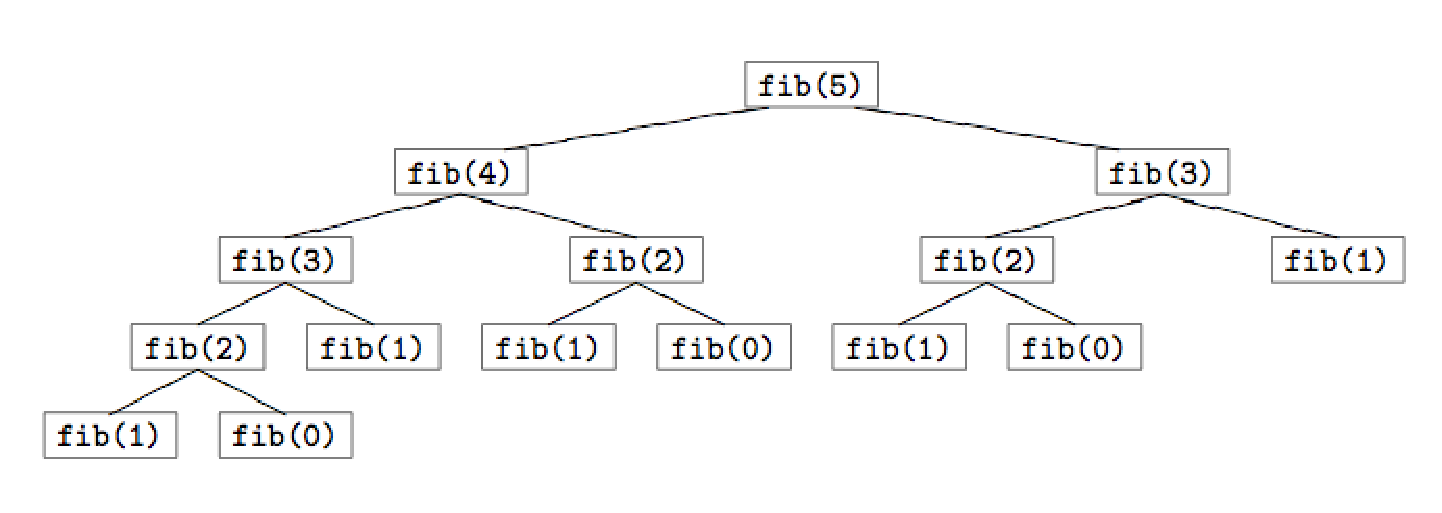
\epsfig{file=fibonacci.eps, scale=0.6}} 
  \caption{Rekursions-Baum f�r die Berechnung von $\textsl{fibonacci}(5)$.}
  \label{fig:fibonacci.eps}
\end{figure}


Wir k�nnen eine effizientere Berechnung der Fibonacci-Zahlen implementieren, indem wir
uns die berechneten Werte merken.  Dazu k�nnen wir in \Java\ ein Feld benutzen.
 Dies f�hrt zu dem in Abbildung \ref{fig:fibonacci-dynamic}
auf Seite \pageref{fig:fibonacci-dynamic} angegebenen Programm.
Da die Werte der Funktion \texttt{fibonacci}() exponentiell wachsen, reichen 32-Bit-Zahlen
nicht aus, um diese Werte darzustellen.  Wir verwenden daher die Klasse
\texttt{BigInteger}, mit der sich ganze Zahlen beliebiger Gr��e darstellen lassen.
Da Felder in \Java\ genau wie in \texttt{C} mit 0 beginnend indiziert werden,
hat ein Feld, dessen oberster Index $n$ ist, insgesamt $n+1$ Elemente.  Wir legen daher in
Zeile 19 ein Feld von $n+1$ Elementen an.

\begin{figure}[!h]
  \centering
\begin{Verbatim}[ frame         = lines, 
                  framesep      = 0.3cm, 
                  labelposition = bottomline,
                  numbers       = left,
                  numbersep     = -0.2cm,
                  xleftmargin   = 0.8cm,
                  xrightmargin  = 0.8cm
                ]
    import java.math.*;
    
    public class FibonacciBig
    {
        public static void main(String[] args) 
        {
            for (int i = 0; i < 100; ++i) {
                BigInteger n = fibonacci(i);
                System.out.println("fib(" + i + ") = " + n);
            }
        }
        
        public static BigInteger fibonacci(int n) 
        {
            if (n <= 2) {
                return BigInteger.valueOf(1);
            }
            BigInteger[] mem = new BigInteger[n+1];
            mem[0] = BigInteger.valueOf(1);  // fibonacci(0) = 1
            mem[1] = BigInteger.valueOf(1);  // fibonacci(1) = 1
            for (int i = 0; i < n - 1; ++i) {
                mem[i + 2] = mem[i].add(mem[i + 1]);
            }
            return mem[n];
        }
    }
\end{Verbatim}
\vspace*{-0.3cm}
  \caption{Berechnung der Fibonacci-Zahlen mit Speicherung der Zwischenwerte.}
  \label{fig:fibonacci-dynamic}
\end{figure} 


\section{Lineare Rekurrenz-Gleichung \label{sec:lineare-RG}}
Wir waren bei der Analyse der Komplexit�t des ersten Programms zur Berechnung der
Fibonacci-Zahlen auf die Gleichung \\[0.1cm]
\hspace*{1.3cm} $a_{i+2} = a_{i+1} + {a_i} + 1$ \quad f�r alle $i \in \mathbb{N}$ \\[0.1cm]
gesto�en. Gleichungen dieser Form treten bei der Analyse der Komplexit�t rekursiver
Programme h�ufig auf. Wir wollen uns daher in diesem Abschnitt n�her mit solchen
Gleichungen besch�ftigen.

\begin{Definition}[Lineare homogene Rekurrenz-Gleichung] \hspace*{\fill} \\
{\em 
  Die \emph{lineare homogene Rekurrenz-Gleichung der Ordnung $k$ mit konstanten Koeffizienten} hat die Form
  \begin{equation}
    \label{eq:lhrg}
  a_{n+k} = c_{k-1} \cdot a_{n+k-1} + c_{k-2} \cdot a_{n+k-2} + \cdots + c_1 \cdot a_{n+1} + c_0 \cdot a_{n}
     \quad \mbox{f�r alle $n \in \N$}. 
  \end{equation}
     In Summen-Schreibweise kann diese Gleichung kompakter als 
     \\[0.1cm]
     \hspace*{1.3cm}
     $a_{n+k} = \sum\limits_{i=0}^{k-1} c_i \cdot a_{n+i}$ \quad f�r alle $n \in \mathbb{N}$
     \\[0.1cm]
     geschreiben werden.
     Zus�tzlich werden \emph{Anfangs-Bedingungen}  
      \\[0.1cm]
      \hspace*{1.3cm}      
      $a_0 = d_0, \cdots, a_{k-1} = d_{k-1}$ 
      \\[0.1cm]
      f�r die Folge $\folge{a_n}$ vorgegeben.    
    \hspace*{\fill} $\Box$
}
\end{Definition}
Durch eine lineare homogene Rekurrenz-Gleichung wird die Folge $(a_n)_{n\in\mathbb{N}}$
eindeutig bestimmt: Die Werte $a_n$ f�r $n < k$ sind durch die Anfangs-Bedingungen gegeben und
alle weiteren Werte k�nnen dann durch die Rekurrenz-Gleichung (\ref{eq:lhrg}) bestimmt werden.
Noch  etwas zur Nomenklatur:
\begin{enumerate}
\item Die Rekurrenz-Gleichung (\ref{eq:lhrg}) hei�t \emph{linear}, weil die Glieder der Folge $(a_n)_n$ nur
      linear in der Gleichung (\ref{eq:lhrg}) auftreten.  Ein Beispiel f�r eine
      Rekurrenz-Gleichung, die nicht linear ist, w�re \\[0.1cm]
      \hspace*{1.3cm} $a_{n+1} = a_n^2$ \quad f�r alle $n \in \mathbb{N}$. \\[0.1cm]
      Nicht-lineare Rekurrenz-Gleichungen sind nur in Spezialf�llen geschlossen l�sbar.
\item Die Rekurrenz-Gleichung (\ref{eq:lhrg}) hei�t \emph{homogen}, weil auf der rechten Seite
      dieser Gleichung kein konstantes Glied mehr auftritt.  Ein Beispiel f�r eine
      Gleichung, die nicht homogen ist (wir sprechen auch von \emph{inhomogenen}
      Rekurrenz-Gleichungen), w�re \\[0.1cm]
      \hspace*{1.3cm} $a_{n+2} = a_{n+1} + a_n + 1$ \quad f�r alle $n \in \mathbb{N}$. \\[0.1cm]
      Mit inhomogenen Rekurrenz-Gleichungen werden wir uns sp�ter noch besch�ftigen.
\item Die Rekurrenz-Gleichung (\ref{eq:lhrg}) hat \emph{konstante Koeffizienten}, weil die
      Werte $c_i$ Konstanten sind, die nicht von dem Index $n$ abh�ngen.  Ein Beispiel f�r
      eine Rekurrenz-Gleichung, die keine konstanten Koeffizienten hat, ist \\[0.1cm]
      \hspace*{1.3cm} $a_{n+1} = n\cdot a_n$ \quad f�r alle $n \in \mathbb{N}$. \\[0.1cm]
      Solche Rekurrenz-Gleichungen k�nnen in vielen F�llen auf Rekurrenz-Gleichungen mit
      konstanten Koeffizienten zur�ck gef�hrt werden.  Wir werden das sp�ter noch im
      Detail besprechen.
\end{enumerate}
Wie l�sen wir eine lineare homogene Rekurrenz-Gleichung?  Wir versuchen zun�chst den Ansatz\\[0.1cm]
\hspace*{1.3cm}  $a_n = \lambda^n$ \quad f�r alle $n \in \mathbb{N}$. \\[0.1cm]
Einsetzen dieses Ansatzes in (\ref{eq:lhrg}) f�hrt auf die Gleichung \\[0.1cm]
\hspace*{1.3cm}
$\lambda^{n+k} = \sum\limits_{i=0}^{k-1} c_i \cdot \lambda^{n+i}$
\\[0.1cm]
Dividieren wir diese Gleichung durch $\lambda^n$, so haben wir: \\[0.1cm]
\hspace*{1.3cm} $\lambda^{k} = \sum\limits_{i=0}^{k-1} c_i \cdot \lambda^{i}$  
\\[0.1cm]
Das Polynom \\[0.1cm]
\hspace*{1.3cm} 
$\chi(x) = x^{k} - \sum\limits_{i=0}^{k-1} c_i \cdot x^{i}$  
\\[0.1cm]
 hei�t \emph{charakteristisches Polynom} der Rekurrenz-Gleichung (\ref{eq:lhrg}).
Wir betrachten zun�chst den Fall, dass das charakteristische  Polynom  $k$  verschiedene
Nullstellen hat.  In diesem Fall sagen, dass die Rekurrenz-Gleichung (\ref{eq:lhrg}) 
\emph{nicht entartet} ist.
Bezeichnen wir diese Nullstellen mit \\[0.1cm]
\hspace*{1.3cm}  $\lambda_1$, $\lambda_2$, $\cdots$, $\lambda_k$, \\[0.1cm]
so  gilt f�r alle $j = 1,\cdots, k$ \\[0.1cm]
\hspace*{1.3cm} 
$\lambda_j^{n+k} = \sum\limits_{i=0}^{k-1} c_i \cdot \lambda_j^{n+i}$.
\\[0.1cm]
Damit ist die Folge  
\[\bigl(\lambda_j^n)_{n\in\mathbb{N}}\]
f�r alle $j=1,\cdots,k$ eine L�sung der Rekurrenz-Gleichung (\ref{eq:lhrg}).
Au�erdem ist auch jede Linear-Kombination dieser L�sungen eine L�sung von (\ref{eq:lhrg}):
Definieren wir die Folge $a_n$ durch \\[0.1cm]
\hspace*{1.3cm} $a_n = \alpha_1 \lambda_1^n + \cdots + \alpha_k \lambda_k^n$ \quad f�r alle $n \in \mathbb{N}$ \\[0.1cm]
mit beliebigen Koeffizienten $\alpha_i \in \R$, so erf�llt auch die Folge
$(a_n)_n$ die Gleichung (\ref{eq:lhrg}).  Die oben definierte Folge $(a_n)_n$ bezeichnen wir als
die  \emph{allgemeine L�sung} der Rekurrenz-Gleichung (\ref{eq:lhrg}): \\[0.1cm]
Die Koeffizienten $\alpha_1$ bis $\alpha_k$ m�ssen wir nun so w�hlen, dass die
Anfangs-Bedingungen 
\\[0.2cm]
\hspace*{1.3cm}
$a_0 = d_0$, $\cdots$, $a_{k-1} = d_{k-1}$
\\[0.2cm]
erf�llt sind.  Das liefert ein lineares Gleichungs-System f�r die Koeffizienten $\alpha_1$, $\cdots$, $\alpha_k$:
\[
\begin{array}{lcl}
  d_0     & = & \lambda_1^0 \cdot \alpha_1 + \cdots +   \lambda_k^0 \cdot \alpha_k \\[0.1cm]
  d_1     & = & \lambda_1^1 \cdot \alpha_1 + \cdots +   \lambda_k^1 \cdot \alpha_k \\[0.1cm]
  \vdots  &   & \vdots                                                   \\[0.1cm]
  d_{k-1} & = & \lambda_1^{k-1} \cdot \alpha_1 + \cdots +   \lambda_{k}^{k-1} \cdot \alpha_k \\[0.1cm]
\end{array}
\]
Hier sind die Werte $\lambda_i$  die Nullstellen des charakteristischen Polynoms.  
Die Matrix $V$, die diesem Gleichungs-System
zugeordnet ist, lautet: 
\[
V = \left(
\begin{array}{lcl}
  \lambda_1^0  & \cdots &   \lambda_k^0 \\[0.1cm]
  \lambda_1^1  & \cdots &   \lambda_k^1 \\[0.1cm]
  \vdots         &         & \vdots \\[0.1cm]
  \lambda_1^{k-1} & \cdots &   \lambda_{k}^{k-1} \\[0.1cm]
\end{array}\right)
\]
Diese Matrix ist in der Mathematik als \emph{Vandermonde}'sche Matrix bekannt.  F�r die
Determinate dieser Matrix gilt \\[0.1cm]
\hspace*{1.3cm} $\det(V) = \prod\limits_{1 \leq i < j \leq k} (\lambda_i - \lambda_j)$. \\[0.1cm]
Sind die Nullstellen $\lambda_i$ f�r $i=1,\cdots,k$ paarweise verschieden, so ist jeder
der Faktoren $(\lambda_i - \lambda_j)$ von 0 verschieden und damit ist auch das Produkt
von 0 verschieden.  Daraus folgt, das das zugeh�rige lineare Gleichungs-System eindeutig
l�sbar ist.  Mit der L�sung dieses Gleichungs-Systems
 haben wir dann die L�sung der Rekurrenz-Gleichung (\ref{eq:lhrg}) gefunden.
\vspace*{0.1cm}

\noindent
\textbf{Beispiel}:  Wie demonstrieren das Verfahren an einem Beispiel: Wie betrachten die
Rekurrenz-Gleichung \\[0.1cm]
\hspace*{1.3cm} $F_{n+2} = F_{n+1} + F_{n}$ \quad f�r alle $n \in \mathbb{N}$  \\[0.1cm]
mit den Anfangs-Bedingungen $F_0 = 0$ und $F_1 = 1$.  Die L�sung dieser
Rekurrenz-Gleichung sind �brigens gerade die Fibonacci-Zahlen.
Das \emph{charakteristische Polynom} dieser Rekurrenz-Gleichung lautet: \\[0.1cm]
\hspace*{1.3cm} $\chi(x) = x^2 - x - 1$.  \\[0.1cm]
Das f�hrt auf die quadratische Gleichung \\[0.1cm]
\hspace*{1.3cm} $x^2 -x - 1 = 0$ \\[0.1cm]
Wir haben eben schon gesehen, dass diese quadratische Gleichung die L�sung \\[0.1cm]
\hspace*{1.3cm}
 $ x_{1/2} = \frac{1}{2} \cdot (1 \pm \sqrt{5})$ 
\\[0.1cm]
hat.  Wir definieren \\[0.1cm]
\hspace*{1.3cm} 
$\lambda_1 = \frac{1}{2} \cdot (1 + \sqrt{5})$ \quad und  \quad 
$\lambda_2 = \frac{1}{2} \cdot (1 - \sqrt{5})$. \\[0.1cm]
Damit lautet die \emph{allgemeine L�sung} der betrachteten Rekurrenz-Gleichung \\[0.1cm]
\hspace*{1.3cm}  $F_n = \alpha_1 \cdot \lambda_1^n  + \alpha_2 \cdot \lambda_2^n$ \quad f�r alle $n \in \mathbb{N}$. \\[0.1cm]
Setzen wir hier die Anfangs-Bedingungen ein, so erhalten wir
\[
\begin{array}{lcl}
    0 & = & \lambda_1^0 \cdot \alpha_1 + \lambda_2^0   \cdot \alpha_2 \\[0.1cm]
    1 & = & \lambda_1^1 \cdot \alpha_1 + \lambda_2^{1} \cdot \alpha_2 
\end{array}
\]
Dies ist ein lineares Gleichungs-System in den Unbekannten $\alpha_1$ und
$\alpha_2$. Vereinfachung f�hrt auf 
\[
\begin{array}{lcl}
    0 & = & \alpha_1 + \alpha_2 \\[0.1cm]
    1 & = & \lambda_1 \cdot \alpha_1 + \lambda_2 \cdot \alpha_2 
\end{array}
\]
Die erste dieser beiden Gleichungen l�sen wir nach $\alpha_2$ auf und finden  $\alpha_2 = - \alpha_1$.
Diesen Wert setzen wir in der zweiten Gleichung ein.  Das f�hrt auf
\[
\begin{array}{lrcl}
                 & 1 & = & \lambda_1 \cdot \alpha_1 - \lambda_2 \cdot \alpha_1 \\
 \Leftrightarrow & 1 & = & (\lambda_1 - \lambda_2) \cdot \alpha_1 \\
 \Leftrightarrow & \bruch{1}{\lambda_1 - \lambda_2} & = & \alpha_1 \\
\end{array}
\]
Setzen wir diesen Wert in der Gleichung $\alpha_2 = - \alpha_1$ ein, so erhalten wir \\[0.1cm]
\hspace*{1.3cm} 
  $\alpha_2 = \bruch{- 1}{\lambda_1 - \lambda_2}$.
\\[0.1cm]
Setzen wir die  Werte f�r $\lambda_1$ und $\lambda_2$ ein, so finden wir:  \\[0.1cm]
\hspace*{1.3cm} 
$\alpha_1 = \bruch{1}{\sqrt{5}}$ \quad und \quad $\alpha_2 = - \bruch{1}{\sqrt{5}}$.
\\[0.1cm]
Die L�sung der Rekurrenz-Gleichung \\[0.1cm]
\hspace*{1.3cm} $F_{n+2} = F_{n+1} + F_{n}$ \quad f�r alle $n \in \mathbb{N}$ \\[0.1cm]
mit den Anfangs-Bedingungen $F_0 = 1$ und $F_1 = 1$   lautet also 
\\[0.1cm]
\hspace*{1.3cm} 
$F_n = \bruch{1}{\sqrt{5}}\cdot \left( \lambda_1^{n} - \lambda_2^{n} \right)$ 
\quad f�r alle $n \in \mathbb{N}$.  
\\[0.1cm]
Damit haben wir eine geschlossene Formel zur Berechnung der Fibonacci-Zahlen
gefunden.  Diese Formel zeigt uns, dass die Fibonacci-Zahlen selbst exponentiell anwachsen.
Wir werden diese L�sung bei der Analyse des Euklidischen-Algorithmus ben�tigen.

\vspace*{0.2cm}
\noindent
\textbf{Aufgabe}:  L�sen Sie die Rekurrenz-Gleichung 
$a_{n+2} = \bruch{3}{2} \cdot a_{n+1} - \bruch{1}{2}\cdot a_n$ mit
den Anfangs-Bedingungen $a_0 = 3$ und $a_1 = \bruch{5}{2}$.

%\noindent
%\textbf{L�sung}: $a_n = 2 + \left(\frac{1}{2}\right)^n$.

\subsection{Entartete Rekurrenz-Gleichungen}
Wir hatten oben zun�chst den Fall betrachtet, dass das charakteristische Polynom der
Rekurrenz-Gleichung (\ref{eq:lhrg}) insgesamt $k$ verschiedene Nullstellen hat.   Dies muss
keineswegs immer der Fall sein.  Wir betrachten die Rekurrenz-Gleichung 
\begin{equation}
  \label{eq:erg}
  a_{n+2} = 4 \cdot a_{n+1} - 4 \cdot a_n \quad \mbox{f�r alle $n \in \mathbb{N}$} 
\end{equation}
 mit den Anfangs-Bedingungen $a_0 = 1$, $a_1 = 4$.  Das charakteristische Polynom lautet \\[0.1cm]
\hspace*{1.3cm} $\chi(x) = x^2 - 4 \cdot x + 4 = (x - 2)^2$ \\[0.1cm]
und hat offensichtlich nur eine Nullstelle bei $x = 2$.   Eine L�sung der
Rekurrenz-Gleichung (\ref{eq:erg}) lautet daher \\[0.1cm]
\hspace*{1.3cm} $a_n = 2^n$ \quad f�r alle $n \in \mathbb{N}$. \\[0.1cm]
Eine weitere L�sung ist \\[0.1cm]
\hspace*{1.3cm} $a_n = n \cdot 2^n$ \quad f�r alle $n \in \mathbb{N}$.  \\[0.1cm]
Wir verifizieren dies durch Einsetzen: 
\[
\begin{array}{llcll}
 & (n+2) \cdot 2^{n+2} & = & 4 \cdot (n+1) \cdot 2^{n+1} - 4 \cdot n \cdot 2^n & \mid\; \div 2^n \\
\Leftrightarrow & 
   (n+2) \cdot 2^{2} & = & 4 \cdot (n+1) \cdot 2^{1} - 4 \cdot n  &  \mid\; \div 4 \\
\Leftrightarrow & n + 2 & = & (n + 1) \cdot 2 -  n  &  \\
\Leftrightarrow & n + 2 & = & 2 \cdot n + 2 -  n   \\
\Leftrightarrow & n + 2 & = & n + 2    \\
\end{array}
\]
Die allgemeine L�sung der Rekurrenz-Gleichung finden wir durch Linear-Kombination der
beiden L�sungen: \\[0.1cm]
\hspace*{1.3cm} $a_n = \alpha \cdot 2^n + \beta \cdot n \cdot 2^n$ \quad f�r alle $n \in \mathbb{N}$. \\[0.1cm]
Setzen wir hier die Anfangs-Bedingungen $a_0 = 1$ und $a_2 = 4$ ein, so erhalten wir:
\[
\left\{
\begin{array}{lcl}
  1 & = & \alpha \cdot 2^0 + \beta \cdot 0 \cdot 2^0 \\
  4 & = & \alpha \cdot 2^1 + \beta \cdot 1 \cdot 2^1 \\
\end{array}
\right\} \quad\Leftrightarrow\quad \left\{
\begin{array}{lcl}
  1 & = & \alpha \\
  4 & = & \alpha \cdot 2 + \beta \cdot 2 \\
\end{array}
\right\}\]
Die L�sung lautet offenbar $\alpha = 1$ und $\beta = 1$.  Damit lautet die L�sung der
Rekurrenz-Gleichung (\ref{eq:erg}) mit den Anfangs-Bedingungen $a_0 = 1$ und $a_2 = 4$ \\[0.1cm]
\hspace*{1.3cm} $a_n = 2^n + n \cdot 2^n = (n+1) \cdot 2^n$ \quad f�r alle $n \in \mathbb{N}$.  \\[0.1cm]
Im allgemeinen nennen wir die Rekurrenz-Gleichung \\[0.1cm]
\hspace*{1.3cm} $a_{n+k} = \sum\limits_{i=0}^{k-1} c_{i} \cdot a_{n+i}$ \\[0.1cm]
\emph{entartet}, wenn das charakteristische Polynom \\[0.1cm]
\hspace*{1.3cm} $\chi(x) = x^k - \sum\limits_{i=0}^{k-1} c_{i} \cdot x^{i}$  \\[0.1cm]
weniger als $k$ verschiedene Nullstellen hat.  Dann l�sst sich folgendes
zeigen:  Hat das charakteristische Polynom $\chi(x)$ eine $r$-fache Nullstelle
$\lambda$, gilt also \\[0.1cm]
\hspace*{1.3cm} $\chi(x) = (x - \lambda)^r \cdot \phi(x)$ \\[0.1cm]
mit einem geeigneten Polynom $\phi(x)$, so sind die Folgen
\begin{enumerate}
\item $(\lambda^n)_{n\in\mathbb{N}}$
\item $(n\cdot\lambda^n)_{n\in\mathbb{N}}$
\item $(n^2\cdot\lambda^n)_{n\in\mathbb{N}}$
\item $\vdots$
\item $(n^{r-1}\cdot\lambda^n)_{n\in\mathbb{N}}$
\end{enumerate}
L�sungen der Rekurrenz-Gleichung (\ref{eq:erg}).  Durch eine geeignete Linear-Kombination dieser
L�sungen zusammen mit den L�sungen, die sich aus den Nullstellen des Polynoms $\phi$
ergeben, l�sst sich dann immer eine L�sung finden, die auch den Anfangs-Bedingungen gen�gt.
\vspace*{0.3cm}

\noindent
\textbf{Aufgabe}: L�sen Sie die Rekurrenz-Gleichung \\[0.1cm]
\hspace*{1.3cm} $a_{n+3} = a_{n+2} + a_{n+1} - a_n$ \\[0.1cm]
f�r die Anfangs-Bedingungen $a_0 = 0$, $a_1 = 3$, $a_2 = 2$.

%\noindent
%\textbf{L�sung}: allg. $a_n = \alpha + n \cdot \beta + \gamma \cdot (-1)^n$. 
%Anfangs-Bedingungen: $a_n = 1 + n - (-1)^n$.

\subsection{Inhomogene Rekurrenz-Gleichungen}    
\begin{Definition}[Lineare inhomogene Rekurrenz-Gleichung]
{\em Die \emph{lineare \underline{inhomo}g\underline{ene} Rekur\-renz-Gleichung der Ordnung
$k$ mit konstanten Koeffizienten und konstanter Inhomogenit�t} hat die Form 
\begin{equation}
  \label{eq:lihrg}
     a_{n+k} = \sum\limits_{i=0}^{k-1} c_{i} \cdot a_{n+i} + c_{-1}  
\end{equation}
     mit den Anfangs-Bedingungen $a_0 = d_0$, $\cdots$, $a_{k-1} = d_{k-1}$. 
     Dabei gilt f�r die Koeffizienten \\[0.1cm]
     \hspace*{1.3cm} $c_i \in \R$ \quad f�r alle $i = -1, 0,\cdots, k-1$. \\[0.1cm]
     F�r die  \emph{Anfangs-Bedingungen} $d_0, \cdots, d_{k-1}$ gilt ebenfalls \\[0.1cm]
     \hspace*{1.3cm} $d_i \in \R$ \quad f�r alle $i = 0,\cdots, k-1$. \\[0.1cm]
     Die Konstante $c_{-1}$ bezeichnen wir als die \emph{Inhomogenit�t}. 
     \hspace*{\fill} $\Box$
}
\end{Definition}

Wie l�sst sich die inhomogene Rekurrenz-Gleichung (\ref{eq:lihrg}) l�sen? Wir zeigen
zun�chst, wie sich eine \emph{spezielle L�sung} der Rekurrenz-Gleichung (\ref{eq:lihrg})
finden l�sst.  Dazu betrachten wir das charakteristische Polynom \\[0.1cm]
\hspace*{1.3cm} 
$\chi(x) = x^k - \sum\limits_{i=0}^{k-1} c_{i} \cdot x^i$
\\[0.1cm]
und definieren die \emph{Spur} $\mathtt{sp}(\chi)$ wie folgt: \\[0.1cm]
\hspace*{1.3cm} 
$\mathtt{sp}(\chi) := \chi(1) = 1 - \sum\limits_{i=0}^{k-1} c_{i}$. \\[0.1cm]
Es k�nnen zwei F�lle auftreten, $\mathtt{sp}(\chi) \not= 0$ und
$\mathtt{sp}(\chi) = 0$.
Wir betrachten die beiden F�lle getrennt.
\begin{enumerate}
\item $\mathtt{sp}(\chi) \not= 0$.

      Dann erhalten wir eine spezielle L�sung von (\ref{eq:lihrg}) durch den Ansatz \\[0.1cm]
      \hspace*{1.3cm} $a_n = \delta$ \quad f�r alle $n \in \mathbb{N}$. \\[0.1cm]
      Den Wert von $\delta$ bestimmen wir durch Einsetzen, es muss f�r alle $n\in \mathbb{N}$ gelten: \\[0.1cm]
      \hspace*{1.3cm} 
      $\delta = \sum\limits_{i=0}^{k-1} c_{i} \cdot \delta + c_{-1}$.
      \\[0.1cm]
      Daraus ergibt sich \\[0.1cm]
      \hspace*{1.3cm} 
      $\delta \cdot \left(1 - \sum\limits_{i=0}^{k-1} c_{i} \right) =  c_{-1}$. \\[0.1cm]
      Das ist aber nichts anderes als \\[0.1cm]
      \hspace*{1.3cm} $\delta \cdot \mathtt{sp}(\chi) = c_{-1}$ \\[0.1cm]
      und damit lautet eine spezielle L�sung von (\ref{eq:lihrg}) \\[0.1cm]
      \hspace*{1.3cm} $a_n = \delta = \bruch{c_{-1}}{\mathtt{sp}(\chi)}$.
      \\[0.1cm]
      Jetzt sehen wir auch, warum die Voraussetzung $\mathtt{sp}(\chi) \not= 0$
      wichtig ist, denn anderfalls w�re der Quotient
      $\bruch{c_{-1}}{\mathtt{sp}(\chi)}$ undefiniert.
\item $\mathtt{sp}(\chi) = 0$.

      In diesem Fall versuchen wir, eine spezielle L�sung von (\ref{eq:lihrg}) durch den
      Ansatz \\[0.1cm]
      \hspace*{1.3cm} $a_n = \varepsilon \cdot n $ \\[0.1cm]
      zu finden.  Den Wert $\varepsilon$ erhalten wir durch Einsetzen, es muss f�r 
      alle $n\in\mathbb{N}$ gelten: \\[0.1cm]
      \hspace*{1.3cm} 
      $\varepsilon \cdot (n + k) = \sum\limits_{i=0}^{k-1} c_{i} \cdot \varepsilon \cdot (n + i) + c_{-1}$  
      \\[0.1cm]
      Dies formen wir wie folgt um:
      \[
        \varepsilon \cdot n + \varepsilon \cdot k = 
        \varepsilon \cdot n \cdot \sum\limits_{i=0}^{k-1} c_{i} +
        \varepsilon \cdot \sum\limits_{i=0}^{k-1} i \cdot c_{i} + c_{-1} 
      \]
      Aus  $\mathtt{sp}(\chi) = 0$ folgt $1  =  \sum\limits_{i=0}^{k-1} c_i$
      und damit gilt \\[0.1cm]
      \hspace*{1.3cm} 
      $\varepsilon \cdot n = \varepsilon \cdot n \cdot \sum\limits_{i=0}^{k-1} c_{i}$.
      \\[0.1cm]
      Daher vereinfacht sich die obige Gleichung zu 
      \[
      \begin{array}{ll}
      & \varepsilon \cdot k = \varepsilon \cdot \sum\limits_{i=0}^{k-1} i \cdot c_{i} + c_{-1} \\[0.4cm]
      \Leftrightarrow\quad 
      & \varepsilon \cdot \left(k - \sum\limits_{i=0}^{k-1} i \cdot c_{i}\right) = c_{-1} 
      \\[0.5cm]
      \Leftrightarrow\quad 
      & \varepsilon = \frac{\displaystyle c_{-1}}{\displaystyle \; k - \sum\limits_{i=0}^{k-1} i \cdot c_{i}\;} 
      \end{array}
      \]
      Wenn wir genau hin schauen, dann sehen wir, dass der Wert im Nenner nicht anderes ist
      als der Wert der Ableitung des charakteristischen Polynoms an der Stelle 1, denn es gilt: \\[0.1cm]
      \hspace*{1.3cm} 
      $\chi'(x) =\bruch{d\,\chi(x)}{dx} = k \cdot x^{k-1} - \sum\limits_{i=0}^{k-1} c_{i}\cdot i \cdot x^{i-1}$
      \\[0.1cm]
      Setzen wir hier f�r $x$ den Wert $1$ ein, so finden wir \\[0.1cm]
      \hspace*{1.3cm} 
      $\chi'(1) = k - \sum\limits_{i=0}^{k-1} c_{i}\cdot i$. 
      \\[0.1cm]
      Insgesamt haben wir damit also die folgende spezielle L�sung $(a_n)_{n\in\mathbb{N}}$
      der Gleichung (\ref{eq:lihrg}) gefunden: \\[0.1cm]
      \hspace*{1.3cm} $a_n = \bruch{c_{-1}}{\;\chi'(1)\;}\cdot n$.

      Wir haben oben zur Vereinfachung angenommen, dass dieser Wert von 0 verschieden ist,
      dass also das charakteristische Polynom $\chi(x)$ an der Stelle $x=1$ keine mehrfache
      Nullstelle hat, denn nur dann ist $\varepsilon$ durch die
      obige Gleichung wohldefiniert und wir haben eine spezielle L�sung der
      Rekurrenz-Gleichung (\ref{eq:lihrg}) gefunden.  Andernfalls k�nnen wir die Reihe nach die
      Ans�tze $a_n = \varepsilon \cdot n^2$, $a_n = \varepsilon \cdot n^3$ , $\cdots$
      versuchen, denn es kann folgendes gezeigt werden: 
      Hat das charakteristische Polynom $\chi(x)$ am Punkt $x = 1$ eine Nullstelle vom Rang $r$,
      so f�hrt der Ansatz $a_n = \varepsilon \cdot n^r$ zu einer speziellen L�sung von (\ref{eq:lihrg}).
\end{enumerate}
Diese spezielle L�sung gen�gt i.~a.~noch nicht den
Anfangs-Bedingungen. Eine L�sung, die auch den Anfangs-Bedingungen gen�gt, erhalten wir,
wenn wir zu der speziellen L�sung die allgemeine L�sung der zugeh�rigen homogenen linearen
Rekurrenz-Gleichung \\[0.1cm]
\hspace*{1.3cm} 
     $a_{n+k} = c_{k-1} \cdot a_{n+k-1} + c_{k-2} \cdot a_{n+k-2} + \cdots + c_1 \cdot a_{n+1} + c_0 \cdot a_{n}$ 
\\[0.1cm]
addieren und die Koeffizienten der allgemeinen L�sung so w�hlen, dass die
Anfangs-Bedingungen erf�llt sind.  Wir betrachten  ein Beispiel:
 Die zu l�sende Rekurrenz-Gleichung lautet \\[0.1cm]
\hspace*{1.3cm} $a_{n+2} = 3 \cdot a_{n+1} - 2 \cdot a_n -1$ \quad f�r alle $n \in \mathbb{N}$. \\[0.1cm]
Die Anfangs-Bedingungen sind $a_0 = 1$ und $a_1 = 3$.  Wir berechnen zun�chst eine
spezielle L�sung.  Das charakteristische Polynom ist \\[0.1cm]
\hspace*{1.3cm} $\chi(x) = x^2 -3 \cdot x +2 = (x - 1) \cdot (x - 2)$. \\[0.1cm]
Es gilt $\mathtt{sp}(\chi) = \chi(1) = 0$.  Wir versuchen f�r die spezielle L�sung
den Ansatz \\[0.1cm]
\hspace*{1.3cm} $a_n = \varepsilon \cdot n$. \\[0.1cm]
Einsetzen in die Rekurrenz-Gleichung liefert \\[0.1cm]
\hspace*{1.3cm}  $\varepsilon \cdot (n+2) = 3 \cdot \varepsilon \cdot(n+1) - 2 \cdot \varepsilon \cdot n -1$ \quad f�r alle $n \in \mathbb{N}$. \\[0.1cm]
Das ist �quivalent zu \\[0.1cm]
\hspace*{1.3cm} $\varepsilon \cdot (2 - 3) = - 1$ \\[0.1cm]
und daraus folgt sofort $\varepsilon = 1$.  Damit lautet eine spezielle L�sung \\[0.1cm]
\hspace*{1.3cm} $a_n = n$ \quad f�r alle $n \in \mathbb{N}$. \\[0.1cm]
Da die Nullstellen des charakteristischen Polynoms $\chi(x)$ bei 1 und 2 liegen, finden
wir f�r die allgemeine L�sung 
\\[0.1cm]
\hspace*{1.3cm} $a_n = \alpha \cdot 1^n + \beta \cdot 2^n + n$ \quad f�r alle $n \in \mathbb{N}$. \\[0.1cm]
Setzen wir hier f�r $n$ die Werte $0$ und $1$ und f�r $a_n$ die beiden Anfangs-Bedingungen
ein, so erhalten wir das Gleichungs-System \\[0.1cm]
\[ \left\{
\begin{array}{lcl}
1 &=& \alpha \cdot 1^0 + \beta \cdot 2^0 + 0 \\
3 &=& \alpha \cdot 1^1 + \beta \cdot 2^1 + 1
\end{array} \right\} \Leftrightarrow \left\{
\begin{array}{lcl}
1 &=& \alpha + \beta  \\
3 &=& \alpha + 2 \cdot \beta + 1
\end{array} \right\}\]
Sie k�nnen leicht nachrechnen, dass dieses Gleichungs-System die L�sung $\alpha = 0$ und
$\beta = 1$ hat.  Damit lautet die L�sung der Rekurrenz-Gleichung \\[0.1cm]
\hspace*{1.3cm} $a_n = 2^n + n$ \quad f�r alle $n \in \mathbb{N}$.
\vspace*{0.3cm}

\noindent
\textbf{Aufgabe}: L�sen Sie die inhomogene Rekurrenz-Gleichung \\[0.1cm]
\hspace*{1.3cm} $a_{n+2} = 2 \cdot a_n - a_{n+1} + 3$ \\[0.1cm]
f�r die Anfangs-Bedingungen $a_0 = 2$ und $a_1 = 1$.
% charakteristisches Polynom: $\chi(x) = x^2 + x - 2 = (x - 1) * (x + 2)
% sp(\chi) = 0, \chi'(x) = 2*x + 1, \chi'(1) = 3
% Lsg: a_n = \varepsilon * n mit \varepsilon = 1
% Lsg: a_n = 4/3 + 2/3*(-2)^n + n
\pagebreak

\subsection{Lineare inhomogene Rekurrenz-Gleichungen mit ver�nderlichen Inhomogenit�ten}
Gelegentlich tauchen in der Praxis Rekurrenz-Gleichungen auf, in denen die Inhomogenit�t
keine Konstante ist, sondern von $n$ abh�ngt.  In solchen F�llen f�hrt die
Technik des \emph{diskreten Differenzieren} oft zum Erfolg.  Wir stellen die Technik an
einem Beispiel vor und betrachten die Rekurrenz-Gleichung 
\begin{equation}
  \label{eq:dd}
a_{n+1} = 2 \cdot a_n + n \quad \mbox{f�r alle $n \in \mathbb{N}$}  
\end{equation}
und der Anfangs-Bedingungen $a_0 = 0$.  Das Verfahren zur L�sung solcher
Rekurrenz-Gleichung besteht aus vier Schritten:
\begin{enumerate}
\item Substitutions-Schritt: Im \emph{Substitutions-Schritt} setzen wir in der
      urspr�nglichen Rekurrenz-Gleichung (\ref{eq:dd}) f�r $n$ den Wert $n + 1$ ein und
      erhalten 
      \begin{equation}
        \label{eq:dd2}
        a_{n+2} = 2 \cdot a_{n+1} + n + 1 \quad \mbox{f�r alle $n \in \N$}
      \end{equation}
\item Subtraktions-Schritt: Im \emph{Subtraktions-Schritt} ziehen wir von der im
      Substitutions-Schritt erhaltenen Rekurrenz-Gleichung (\ref{eq:dd2}) die urspr�ngliche
      gegebene Rekurrenz-Gleichung (\ref{eq:dd}) ab.  In unserem Fall erhalten wir \\[0.1cm]
      \hspace*{1.3cm} 
      $a_{n+2} - a_{n+1} = 2 \cdot a_{n+1} + n + 1 - \left( 2 \cdot a_n + n \right)$ 
      \quad f�r alle $n \in \mathbb{N}$.       \\[0.1cm]
      Vereinfachung dieser Gleichung liefert 
      \begin{equation}
        \label{eq:dd3}
        a_{n+2} = 3 \cdot a_{n+1} - 2 \cdot a_n + 1 \quad \mbox{f�r alle $n \in \N$}.
      \end{equation}
      Die beiden Schritte 1. und 2. bezeichnen wir zusammen als 
      \emph{diskretes Differenzieren} der Rekurrenz-Gleichung.
\item Berechnung zus�tzlicher Anfangs-Bedingungen: Die Rekurrenz-Gleichung (\ref{eq:dd3})
      ist eine inhomogene Rekurrenz-Gleichung der Ordnung 2 mit nun aber konstanter
      Inhomogenit�t.  Wir haben bereits gesehen, 
      wie eine solche Rekurrenz-Gleichung zu l�sen ist, wir ben�tigen aber eine
      zus�tzliche Anfangs-Bedingung f�r $n=1$.  Diese erhalten wir, indem wir in der
      urspr�nglichen Rekurrenz-Gleichung (\ref{eq:dd}) f�r $n$ den Wert 0 einsetzen: \\[0.1cm]
      \hspace*{1.3cm} $a_1 = 2 \cdot a_0 + 0 = 0$.
\item L�sen der inhomogenen Rekurrenz-Gleichung mit konstanter Inhomogenit�t:
      Das charakteristische Polynom der Rekurrenz-Gleichung (\ref{eq:dd3}) lautet: \\[0.1cm]
      \hspace*{1.3cm} $\chi(x) = x^2 - 3 \cdot x + 2 = (x - 2) \cdot (x - 1)$. \\[0.1cm]
      Offenbar gilt $\mathtt{sp}(\chi) = 0$.  Um eine spezielle L�sung der
      Rekurrenz-Gleichung
      (\ref{eq:dd3}) zu erhalten, machen wir daher den Ansatz \\[0.1cm]
      \hspace*{1.3cm} $a_n = \varepsilon \cdot n$ \\[0.1cm]
      und erhalten \\[0.1cm]
      \hspace*{1.3cm} 
      $\varepsilon \cdot (n+2) = 3 \cdot \varepsilon \cdot (n+1) - 2 \cdot \varepsilon \cdot n + 1$ 
      \\[0.1cm]
      Diese Gleichung liefert die L�sung \\[0.1cm]
      \hspace*{1.3cm} 
      $\varepsilon = -1$. \\[0.1cm]
      Damit lautet die allgemeine L�sung der Rekurrenz-Gleichung (\ref{eq:dd3}): \\[0.1cm]
      \hspace*{1.3cm} $a_n = \alpha_1 \cdot 2^n + \alpha_2 \cdot 1^n - n$ \\[0.1cm]
      Die Koeffizienten $\alpha_1$ und $\alpha_2$ finden wir nun durch Einsetzen der
      Anfangs-Bedingungen:
      \[
      \begin{array}{lcl}
        0 & = & \alpha_1 + \alpha_2 \\
        0 & = & 2 \cdot \alpha_1 + \alpha_2 - 1 \\
      \end{array}
      \]
      Aus der ersten Gleichung folgt $\alpha_2 = - \alpha_1$.  Damit vereinfacht sich die
      zweite Gleichung zu \\[0.1cm]
      \hspace*{1.3cm} $0 = 2 \cdot \alpha_1 - \alpha_1 - 1$ \\[0.1cm]
      und damit lautet die L�sung $\alpha_1 = 1$ und $\alpha_2 = -1$.  Die L�sung der
      urspr�nglichen Rekurrenz-Gleichung (\ref{eq:dd}) mit der Anfangs-Bedingung $a_0 = 0$ 
      ist also \\[0.1cm]
      \hspace*{1.3cm} $a_n = 2^n - 1 - n$.
\end{enumerate}
Das oben gezeigte Verfahren funktioniert, wenn die Inhomogenit�t der Rekurrenz-Gleichung
linear ist, also die Form $\delta \cdot n$.  Ist die Inhomogenit�t quadratisch, so k�nnen wir
die Gleichung durch diskretes Differenzieren auf eine Rekurrenz-Gleichung reduzieren,
deren Inhomogenit�t linear ist.  Diese kann dann aber mit dem eben gezeigten Verfahren
gel�st werden.  Allgemein gilt:  Hat die Inhomogenit�t der Rekurrenz-Gleichung die Form \\[0.1cm]
\hspace*{1.3cm} $\delta \cdot n^r$ \quad $r \in \mathbb{N}$ und $r > 0$, \\[0.1cm]
so kann die Rekurrenz-Gleichung durch $r$-maliges diskretes Differenzieren auf eine
inhomogene Rekurrenz-Gleichung mit konstanter Inhomogenit�t reduziert werden.
\vspace*{0.3cm}

\noindent
\textbf{Aufgabe}:  L�sen Sie die Rekurrenz-Gleichung \\[0.1cm]
\hspace*{1.3cm} $a_{n+1} = a_n + 2 \cdot n$ \quad f�r alle $n \in \mathbb{N}$ \\[0.1cm]
mit der Anfangs-Bedingung $a_0 = 0$.
\vspace*{0.3cm}

%\noindent
%\textbf{L�sung}: 
%\begin{enumerate}
%\item Charakteristisches Polynom: $\chi(x) = (x-1)^2$, doppelte Nullstelle! 
%\item Spezielle L�sung: $a_n = n^2$.
%\item Allgemeine L�sung: $a_n = \alpha_1 \cdot 1^n + \alpha_2 \cdot n \cdot 1^n + n^2$
%\item L�sung: $a_n = n\cdot(n-1)$.
%\end{enumerate}

\noindent
Die oben vorgestellte Technik des diskreten Differenzierens f�hrt in leicht variierter
Form oft auch dann noch zu einer L�sung, wenn die Inhomogenit�t nicht die Form eines
Polynoms hat.  Wir betrachten als Beispiel die Rekurrenz-Gleichung 
\begin{equation}
  \label{eq:expdd}
  a_{n+1} = a_n + 2^n \quad \mbox{f�r alle $n \in \N$}
\end{equation}
mit der Anfangs-Bedingungen $a_0 = 0$.   Setzen wir in (\ref{eq:expdd}) f�r $n$ den Wert $n+1$
ein, erhalten wir 
\begin{equation}
  \label{eq:expdd2}
  a_{n+2} = a_{n+1} + 2^{n+1} \quad \mbox{f�r alle $n \in \N$}
\end{equation}
W�rden wir von Gleichung (\ref{eq:expdd2}) die Gleichung (\ref{eq:expdd}) subtrahieren, so w�rde
der Term $2^n$ erhalten bleiben.  Um diesen Term zu eliminieren m�ssen wir statt dessen
von Gleichung (\ref{eq:expdd2}) 2 mal die Gleichung (\ref{eq:expdd})  subtrahieren: \\[0.1cm]
\hspace*{1.3cm}  
$a_{n+2} - 2 \cdot a_{n+1} = a_{n+1} + 2^{n+1} - 2 \cdot \bigl(a_n - 2^n\bigr)$ 
                 \\[0.1cm]
Dies vereinfacht sich zu der homogenen Rekurrenz-Gleichung 
\begin{equation}
  \label{eq:expdd3}
  a_{n+2} = 3 \cdot a_{n+1} - 2 \cdot a_n \quad \mbox{f�r alle $n \in \N$}  
\end{equation}
Das charakteristische Polynom lautet \\[0.1cm]
\hspace*{1.3cm} 
$\chi(x) = x^2 - 3 \cdot x + 2 = (x-1) \cdot (x-2)$.  \\[0.1cm]
Damit lautet die allgemeine L�sung der homogenen Rekurrenz-Gleichung \\[0.1cm]
\hspace*{1.3cm} 
$a_n = \alpha + \beta \cdot 2^n$.  \\[0.1cm]
Da wir hier mit $\alpha$ und $\beta$ zwei Unbekannte haben, brauchen wir eine zus�tzliche
Anfangs-Bedingung.  Diese erhalten wir, indem wir in der Gleichung (\ref{eq:expdd}) f�r $n$
den Wert $0$ einsetzen: \\[0.1cm]
\hspace*{1.3cm} $a_1 = a_0 + 2^0 = 0 + 1 = 1$. \\[0.1cm]
Damit erhalten wir das Gleichungs-System 
\[ 
\begin{array}{lcl}
0 &=& \alpha  + \beta  \\
1 &=& \alpha  + 2 \cdot \beta
\end{array} 
\]
Dieses Gleichungs-System hat die L�sung $\alpha = -1$ und $\beta = 1$.
Damit lautet die L�sung der Rekurrenz-Gleichung (\ref{eq:expdd}) mit der Anfangs-Bedingung
$a_0 = 0$ \\[0.1cm]
\hspace*{1.3cm} $a_n = 2^n - 1$.


\subsection{Die Substitutions-Methode}
Bei der Analyse von Algorithmen, die dem Paradigma \emph{Teile-und-Herrsche} folgen,
treten h�ufig Rekurrenz-Gleichungen auf, bei denen der Wert von $a_n$ von dem Wert von
$a_{n/2}$ oder gelegentlich auch $a_{n/3}$ oder sogar $a_{n/4}$ abh�ngt.  Wir zeigen jetzt
ein Verfahren, mit dessen Hilfe sich auch solche Rekurrenz-Gleichungen behandeln lassen.
Wir demonstrieren das Verfahren an Hand der Rekurrenz-Gleichung 
\begin{equation}
  \label{eq:wrg}
a_n = a_{n/2} + n \quad \mbox{f�r alle $n \in \{ 2^k \mid k \in \N \wedge k \geq 1\}$}  
\end{equation}
mit der Anfangs-Bedingung $a_1 = 0$.   Um diese Rekurrenz-Gleichung zu l�sen, machen wir
den Ansatz \\
\hspace*{1.3cm} $b_k = a_{2^k}$ \quad f�r alle $k \in \mathbb{N}$. \\[0.1cm]
 Setzen wir dies in die
urspr�ngliche Rekurrenz-Gleichung (\ref{eq:wrg}) ein, so erhalten wir \\[0.1cm]
\hspace*{1.3cm} 
$b_{k} = a_{2^{k}} = a_{2^{k}/2} + 2^{k} = a_{2^{k-1}} + 2^{k} = b_{k-1}+ 2^{k}$.
\\[0.1cm]
Setzen wir in dieser Gleichung f�r $k$ den Wert $k+1$ ein, so sehen wir, dass
die Folge $(b_k)_k$ der Rekurrenz-Gleichung 
\begin{equation}
  \label{eq:wrg2}
  b_{k+1} = b_k + 2^{k+1} \quad \mbox{f�r alle $k \in \N$}
\end{equation}
gen�gt.  Dabei ist die Anfangs-Bedingung $b_0 = a_{2^0} = a_1 = 0$.  Das ist eine lineare
inhomogene Rekurrenz-Gleichung mit der Inhomogenit�t $2^{k+1}$. Wir 
setzen in (\ref{eq:wrg2}) f�r $k$ den Wert $k+1$
ein und erhalten 
\begin{equation}
  \label{eq:wrg3}
  b_{k+2} = b_{k+1} + 2^{k+2} \quad \mbox{f�r alle $k \in \N$.}
\end{equation}
Wir multiplizieren nun die Rekurrenz-Gleichung (\ref{eq:wrg2}) mit 2 und ziehen das Ergebnis
von Gleichung  (\ref{eq:wrg3}) ab: \\[0.1cm]
\hspace*{1.3cm} 
$b_{k+2} - 2 \cdot b_{k+1} = b_{k+1} + 2^{k+2} - 2 \cdot b_k - 2 \cdot 2^{k+1}$ \quad f�r alle $k \in \N$. 
\\[0.1cm]
Nach Vereinfachung erhalten wir 
\begin{equation}
  \label{eq:wrg4}
  b_{k+2} = 3 \cdot b_{k+1} - 2 \cdot b_k \quad \mbox{f�r alle $k \in \N$.}
\end{equation}
Die Anfangs-Bedingung f�r $k=1$ berechnen wir aus (\ref{eq:wrg2}) \\[0.1cm]
\hspace*{1.3cm} $b_1 = b_0 + 2^{1} = 0 + 2 = 2$. \\[0.1cm]
Damit haben wir das urspr�ngliche Problem auf eine homogene lineare Rekurrenz-Gleichung
mit konstanten Koeffizienten zur�ck gef�hrt.  Das charakteristische Polynom dieser
Rekurrenz-Gleichung ist \\[0.1cm]
\hspace*{1.3cm} $\chi(x) = x^2 - 3\cdot x + 2 = (x-2)\cdot(x-1)$. \\[0.1cm]
Damit lautet die allgemeine L�sung der Rekurrenz-Gleichung (\ref{eq:wrg4}) \\[0.1cm]
\hspace*{1.3cm} $b_k = \alpha_1 \cdot 2^k + \alpha_2 \cdot 1^k$ \quad f�r alle $k \in \N$. \\[0.1cm]
Wir setzen die Anfangs-Bedingungen ein und erhalten so f�r die Koeffizienten $\alpha_1$
und $\alpha_2$ das lineare Gleichungs-System 
\[
\begin{array}{lcl}
  0 & = & \alpha_1 + \alpha_2 \\
  2 & = & 2 \cdot \alpha_1 + \alpha_2 \\
\end{array}
\]
Ziehen wir die erste Gleichung von der zweiten ab, so sehen wir $\alpha_1 = 2$.  Dann
folgt aus der ersten Gleichung $\alpha_2 = -2$.  Damit haben wir \\[0.1cm]
\hspace*{1.3cm} $b_k = 2^{k+1} - 2$ \quad f�r alle $k \in \N$. \\[0.1cm]
Setzen wir hier $b_k = a_{2^k}$ ein, so finden wir \\[0.1cm]
\hspace*{1.3cm} $a_{2^k} = 2^{k+1} - 2$ \quad f�r alle $k \in \N$. \\[0.1cm]
Mit $n = 2^k$ erhalten wir die L�sung der Rekurrenz-Gleichung (\ref{eq:wrg}) mit der wir 
gestartet waren: \\[0.1cm]
\hspace*{1.3cm} $a_n = 2 \cdot n - 2$ \quad f�r alle $n \in \{ 2^k \mid k \in \N\}$.  
\vspace*{0.3cm}

\noindent
\textbf{Aufgabe}:  L�sen Sie die Rekurrenz-Gleichung \\[0.1cm]
\hspace*{1.3cm} $a_{n} = a_{n/2} + 1$ \quad f�r alle $n \in \{ 2^k \mid k \in \N \wedge k \geq 1\}$\\[0.1cm]
mit der Anfangs-Bedingungen $a_1 = 1$.
\vspace*{0.3cm}

%\noindent
%\textbf{L�sung}:
%\begin{enumerate}
%\item R�ckf�hrung auf $b_{k+1} =  b_k + 1$.
%\item $b_k = k$
%\item $a_n = \log_2(n)$
%\end{enumerate}

\subsection{Das Teleskop-Verfahren}
Bestimmte Rekurrenz-Gleichungen lassen sich auf bereits bekannte Summen zur�ckf�hren.  Wir demonstrieren
das Verfahren an der Rekurrenz-Gleichung \\[0.2cm]
\hspace*{1.3cm} $a_n = a_{n-1} + n - 1$ \quad mit $a_0 = 0$. 
\\[0.2cm]
Diese Gleichung tritt bei der Analyse der Komplexit�t von Quick-Sort auf.
Um diese Gleichung zu l�sen, setzen wir zun�chst f�r $a_{n-1}$ den Wert $a_{n-2} + (n-1) - 1$ ein, dann 
ersetzen wir $a_{n-2}$ durch $a_{n-3} + (n-2) -2$ und fahren so fort, bis wir schlie�lich $a_n$ auf $a_0$
zur�ck gef�hrt haben.
Damit erhalten wir insgesamt:
\[
\begin{array}{lcl}
  a_n & = & a_{n-1} + (n-1) \\
      & = & a_{n-2} + (n-2) + (n-1) \\
      & = & a_{n-3} + (n-3) + (n-2) + (n-1) \\
      & = & \vdots \\
      & = & a_{0} + 0 + 1 + 2 + \cdots  + (n-2) + (n-1) \\
      & = & 0 + 0 + 1 + 2 + \cdots  + (n-2) + (n-1) \\
      & = & \sum\limits_{i=0}^{n-1} i  \\[0.4cm]
      & = &  \frac{1}{2} n \cdot(n - 1) \\[0.2cm]
      & = & \frac{1}{2} \cdot n^2 - \frac{1}{2} \cdot n.
\end{array}
\]
Das eben demonstrierte Verfahren wird in der Literatur als \emph{Teleskop-Verfahren} bezeichnet.  In der
allgemeinen Form des Teleskop-Verfahrens gehen wir von einer Rekurrenz-Gleichung der Form
\\[0.2cm]
\hspace*{1.3cm}
$a_n = a_{n-1} + g(n)$
\\[0.2cm]
aus.  Hierbei ist $g: \mathbb{N} \rightarrow \mathbb{R}$ eine reelwertige Funktion.
Wenden wir das oben demonstrierte Schema an, so erhalten wir die folgende Rechnung:
\[ 
\begin{array}{lcl}  
  a_n & = & a_{n-1} + g(n) \\
      & = & a_{n-2} + g(n-1) + g(n) \\
      & = & a_{n-3} + g(n-2) + g(n-1) + g(n) \\
      & = & \vdots \\
      & = & a_{0} + g(1) + g(2) + \cdots  + g(n-2) + g(n-1) + g(n) \\[0.2cm]
      & = & a_0 + \sum\limits_{i=1}^{n} g(i).
\end{array}
\]
Falls wir in der Lage sind, f�r die Summe $\sum_{i=1}^{n} g(i)$ einen geschlossenen Ausdruck anzugeben,
dann haben wir damit eine L�sung der Rekurrenz-Gleichung $a_n = a_{n-1} + g(n)$
gefunden.

\subsection{Berechnung von Summen}
Der letzte Abschnitt hat gezeigt, dass Rekurrenz-Gleichung in bestimmten F�llen auf Summen zur�ck gef�hrt
werden k�nnen.  In diesem Abschnitt zeigen wir, dass auch der umgekehrte Weg m�glich ist und die  
Berechnung einer Summe auf die L�sung einer Rekurrenz-Gleichung zur�ckgef�hrt werden kann. Wir
demonstrieren das Verfahren am Beispiel der Berechnung der geometrischen Reihe.  Hier wird die Summe
$s_n$ durch die Formel
\begin{equation}
  \label{eq:sum1}
  s_n = \sum\limits_{i=0}^n q^i   
\end{equation}
definiert, wobei wir zur Ersparung von Fallunterscheidungen voraussetzen wollen, dass $q \not= 1$ gilt.
Diese Einschr�nkung ist nicht gravierend denn f�r $q=1$ sehen wir sofort, dass $s_n = n+1$ gilt. Der
erste Schritt besteht darin, dass wir aus der obigen Definition eine Rekurrenz-Gleichung herleiten.
Dies erreichen wir dadurch, dass wir in Gleichung (\ref{eq:sum1}) f�r $n$ den Wert $n+1$ einsetzen.  Wir
erhalten dann die Gleichung
\begin{equation}
  \label{eq:sum2}
  s_{n+1} = \sum\limits_{i=0}^{n+1} q^i    
\end{equation}
Wir bilden nun die Differenz von $s_{n+1} - q * s_n$ und erhalten
\[ s_{n+1} - s_n \cdot q = 1, \]
was wir zu
\[ s_{n+1} = q \cdot s_n + 1 \]
umformen.  Dies ist eine lineare inhomogene Rekurrenz-Gleichung mit konstanter Inhomogenit�t. 
Die Anfangs-Bedingung ist hier offenbar $s_0 = 1$.  Das charakteristische Polynom lautet
\[ \chi(x) = x - q. \]
Diese Polynom hat die Nullstelle $x = q$.  Um die spezielle L�sung der Rekurrenz-Gleichung zu finden,
berechnen wir die Spur des charakteristischen Polynoms.  Es gilt
\[ \mathtt{sp}(\chi) = \chi(1) = 1 - q \not= 0, \]  
denn wir hatten ja $q \not= 1$ vorausgesetzt.  Damit lautet die spezielle L�sung
\[ s_n = \frac{c_{-1}}{\mathtt{sp}(\chi)} = \frac{1}{1 - q}. \]
Folglich lautet die allgemeine L�sung
\[ s_n = \alpha \cdot q^n + \frac{1}{1 - q}.  \]
Um den Koeffizienten $\alpha$ zu bestimmen, setzen wir $n=0$ und erhalten
\[ 1 = \alpha + \frac{1}{1 - q}. \]
L�sen wir diese Gleichung nach $\alpha$ auf, so ergibt sich
\[ \alpha = \frac{(1 - q) - 1}{1 - q} = - \frac{q}{1 - q}. \]
Damit lautet die L�sung
\[ s_n = \frac{1 - q^{n+1}}{1 - q} \]
und wir haben insgesamt die folgende Formel hergeleitet:
\[ \sum\limits_{i=0}^{n} q^i = \frac{1 - q^{n+1}}{1 - q}. \]
\pagebreak

\noindent
\textbf{Aufgabe}:
Berechnen Sie eine geschlossene Formel f�r die Summe
der Quadratzahlen
\[ s_n := \sum\limits_{i=0}^{n} i^2. \]
Stellen Sie dazu eine Rekurrenz-Gleichung f�r $s_n$ auf und l�sen Sie diese.

\subsection{Weitere Rekurrenz-Gleichungen}
Die L�sung allgemeiner Rekurrenz-Gleichungen kann beliebig schwierig sein und
es gibt viele F�lle, in denen eine gegebene Rekurrenz-Gleichungen �berhaupt keine L�sung
hat, die sich durch elementare Funktionen als geschlossene Formel ausdr�cken l�sst.
Wir wollen an Hand einer etwas komplizierteren Rekurrenz-Gleichung, die uns sp�ter bei der Behandlung der
durchschnittlichen Komplexit�t des Quick-Sort-Algorithmus wiederbegegnen wird, zeigen, dass im Allgemeinen bei
der L�sung einer Rekurrenz-Gleichung Kreativit�t gefragt ist.
Wir gehen dazu von der folgenden  Rekurrenz-Gleichung aus:
\begin{equation}
  \label{eq:cqs2}
  d_{n+1} = n + \frac{2}{n+1} \cdot \sum_{i=0}^n d_i.   
\end{equation}
Zun�chst versuchen wir, die Summe $\sum_{i=0}^n d_i$, die auf der rechten Seite dieser Rekurrenz-Gleichung
auftritt, zu eliminieren.  Wir versuchen, analog zu dem Verfahren des diskreten Differenzierens vorzugehen
und substituieren zun�chst $n \mapsto n+1$.  Wir erhalten 
\begin{equation}
  \label{eq:cqs3}
   d_{n+2} = n+1 + \frac{2}{n+2} \cdot \sum_{i=0}^{n+1} d_i.  
\end{equation}
Wir multiplizieren nun Gleichung (\ref{eq:cqs3}) mit $n+2$ und Gleichung (\ref{eq:cqs2}) mit $n+1$ und
haben dann
\begin{eqnarray}
  \label{eq:cqs4}
 (n+2)\cdot d_{n+2} & = & (n+2)\cdot(n+1) + 2 \cdot \sum_{i=0}^{n+1} d_i \qquad \mbox{und} \\
  \label{eq:cqs5}
 (n+1)\cdot d_{n+1} & = & (n+1)\cdot n + 2 \cdot \sum_{i=0}^n d_i.  
\end{eqnarray}
Wir bilden die Differenz der Gleichungen (\ref{eq:cqs4}) und (\ref{eq:cqs5}) und beachten,
dass sich die Summationen bis auf den Term $2\cdot d_{n+1}$ gerade gegenseitig aufheben.
Das liefert
\begin{equation}
  \label{eq:cqs6}
 (n+2)\cdot d_{n+2} - (n+1)\cdot \displaystyle d_{n+1} = (n+2)\cdot(n+1) - (n+1)\cdot n+2 \cdot d_{n+1}.
\end{equation}
Diese Gleichung vereinfachen wir zu
\begin{equation}
  \label{eq:cqs7}
(n+2)\cdot d_{n+2} = (n+3)\cdot \displaystyle d_{n+1} + 2\cdot(n+1).  
\end{equation}
Um diese Gleichung zu homogenisieren teilen wir beide Seiten durch $(n+2) \cdot(n+3)$:
\begin{equation}
  \label{eq:cqs8}
 \frac{1}{n+3} \cdot d_{n+2} = \frac{1}{n+2}\cdot d_{n+1} + \frac{2\cdot(n+1)}{(n+2)\cdot(n+3)}.
\end{equation}
Wir definieren $\displaystyle a_n = \frac{d_n}{n+1}$ und erhalten dann aus der
letzten Gleichung 
\[ a_{n+2} = a_{n+1} + \frac{2\cdot(n+1)}{(n+2)\cdot(n+3)} \]
Die Substitution $n \mapsto n-2$ vereinfacht diese Gleichung zu 
\begin{equation}
  \label{eq:cqs9}
 a_{n} = a_{n-1} + \frac{2\cdot(n-1)}{n\cdot(n+1)}.
\end{equation}
Diese Gleichung k�nnen wir mit dem Teleskop-Verfahren l�sen.  Um die dabei auftretenden Summen �bersichlicher
schreiben zu k�nnen,  bilden wir die Partialbruch-Zerlegung von 
\[ \frac{2\cdot(n-1)}{n\cdot(n+1)}. \] 
Dazu machen wir den Ansatz
\[ \frac{2\cdot(n-1)}{n\cdot(n+1)} = \frac{\alpha}{n} + \frac{\beta}{n+1}.\]
Wir multiplizieren diese Gleichung mit dem Hauptnenner und erhalten
\[ 2\cdot n - 2 = \alpha \cdot (n+1) + \beta \cdot n, \]
was sich zu 
\[ 2\cdot n - 2 = (\alpha + \beta) \cdot n + \alpha \]
vereinfacht.  Ein Koeffizientenvergleich liefert dann das lineare Gleichungs-System
\begin{eqnarray*}
  2 & = & \alpha + \beta, \\
 -2 & = & \alpha.
\end{eqnarray*}
Setzen wir die zweite Gleichung in die erste Gleichung ein, so erhalten wir $\beta = 4$.
Damit k�nnen wir die Gleichung (\ref{eq:cqs9}) als 
\begin{equation}
  \label{eq:cqs10}
 a_{n} = a_{n-1} - \frac{2}{n} + \frac{4}{n+1}  
\end{equation}
schreiben und mit  dem Teleskop-Verfahren l�sen.  Wegen $a_0 = \frac{d_0}{1} = 0$ finden wir
\begin{equation}
  \label{eq:cqs11}
 a_{n} = 4 \cdot \sum_{i=1}^n \frac{1}{i+1} - 2 \cdot \sum_{i=1}^n \frac{1}{i}.  
\end{equation}
Wir vereinfachen diese Summe:
\[
\begin{array}{lcl}
 a_{n} & = & \displaystyle 4 \cdot \sum_{i=1}^n \frac{1}{i+1} - 2 \cdot \sum_{i=1}^n \frac{1}{i} \\[0.5cm]
       & = & \displaystyle 4 \cdot \sum_{i=2}^{n+1} \frac{1}{i} - 2 \cdot \sum_{i=1}^n \frac{1}{i} \\[0.5cm]
       & = & \displaystyle 4 \cdot \frac{1}{n+1} - 4 \cdot \frac{1}{1} + 4 \cdot \sum_{i=1}^{n} \frac{1}{i} - 2 \cdot \sum_{i=1}^n \frac{1}{i} \\[0.5cm]
       & = & \displaystyle 4 \cdot \frac{1}{n+1} - 4 \cdot \frac{1}{1} + 2 \cdot \sum_{i=1}^{n} \frac{1}{i}  \\[0.5cm]
       & = & \displaystyle - \frac{4 \cdot n}{n+1}  + 2 \cdot \sum_{i=1}^{n} \frac{1}{i}  
\end{array}
\]
Um unsere Rechnung abzuschlie�en, berechnen wir eine N�herung f�r die Summe 
\[ H_n = \sum\limits_{i=1}^{n}\frac{1}{i}.\]
Der Wert $H_n$ wird in der Mathematik als die $n$-te \emph{harmonische Zahl} bezeichnet.
Dieser Wert h�ngt mit dem Wert $\ln(n)$ zusammen: Leonhard Euler hat gezeigt, dass f�r
gro�e $n$ die Approximation
\[ \sum\limits_{i=1}^n \frac{1}{i} \approx \ln(n) + \gamma + \frac{1}{2} \cdot \frac{1}{n} \]
benutzt werden kann.  Hier ist $\gamma$ die Euler-Mascheroni'sche Konstante, deren Wert durch
\[ \gamma \approx 0,5772156649 \]
gegeben ist.  Damit haben wir f�r den Wert von $a_n$ die N�herung
\[ a_n = - \frac{4 \cdot n}{n+1} + 2 \cdot H_n \approx  
         2 \cdot \ln(n) + 2 \cdot \gamma - \frac{4 \cdot n}{n+1} + \frac{1}{n} 
\]
gefunden. Wegen $d_n = (n+1) \cdot a_n$ k�nnen wir f�r die Folge $d_n$ also folgendes schreiben:
\[ d_n \approx  
       2 \cdot (n + 1) \cdot \ln(n) + 2 \cdot (n+1) \cdot \gamma - 4 \cdot n + \frac{n+1}{n}.
\]
\vspace*{0.3cm}


Wir verallgemeinern die Idee, die wir bei der L�sung des obigen Beispiels benutzt haben.  Es seien
$f:\mathbb{N} \rightarrow \mathbb{R}$, $g:\mathbb{N} \rightarrow \mathbb{R}$ und 
$h:\mathbb{N} \rightarrow \mathbb{R}$ 
reelwertige Folgen und es sei die Rekurrenz-Gleichung
\[ 
f(n) \cdot a_n = g(n) \cdot a_{n-1} + h(n)
\]
zu l�sen.  Die Idee ist, beide Seiten mit einem geeigneten Faktor, der im Allgemeinen von $n$ abh�ngt, zu
multiplizieren.  Bezeichnen wir diesen Faktor mit $p(n)$, so erhalten wir die Rekurrenz-Gleichung
\[ 
p(n) \cdot f(n) \cdot a_n = p(n) \cdot g(n) \cdot a_{n-1} + p(n) \cdot h(n).
\]
Das Ziel ist dabei, den Faktor $p(n)$ so zu w�hlen, dass der Koeffizient von $a_n$ die selbe Form hat wie der
Koeffizient von $a_{n-1}$, es soll also
\begin{equation}
  \label{eq:chomogen}
  p(n) \cdot g(n) = p(n-1) \cdot f(n-1)  
\end{equation}
gelten, denn dann k�nnen wir die urspr�ngliche Rekurrenz-Gleichung in der Form
\[ 
p(n) \cdot f(n) \cdot a_n = p(n-1) \cdot f(n-1) \cdot a_{n-1} + p(n) \cdot h(n).
\]
schreiben und anschlie�end durch die Substitution $b_n := p(n) \cdot f(n) \cdot a_n$ auf die
Rekurrenz-Gleichung 
\[ 
b_n = b_{n-1} + p(n) \cdot h(n).
\]
Diese Gleichung l�sst sich mit dem Teleskop-Verfahren auf eine Summe zur�ckf�hren und die L�sung der
urspr�nglichen Gleichung kann schlie�lich �ber die Formel
\[ 
a_n = \frac{1}{p(n) \cdot f(n)} \cdot b_n
\]
aus $b_n$ berechnet werden.  Es bleibt also zu kl�ren, wie wir den Faktor $p(n)$ so w�hlen k�nnen, dass
Gleichung (\ref{eq:chomogen}) erf�llt ist. Dazu schreiben wir diese Gleichung als Rekurrenz-Gleichung f�r
$p(n)$ um und erhalten
\[ 
  p(n) = \frac{f(n-1)}{g(n)} \cdot p(n-1) 
\]
Diese Gleichung k�nnen wir mit einer Variante des Teleskop-Verfahrens l�sen:
\[ 
\begin{array}{lcl}
p(n) & = & \frac{f(n-1)}{g(n)} \cdot p(n-1)   \\[0.2cm]
     & = & \frac{f(n-1)}{g(n)} \cdot  \frac{f(n-2)}{g(n-1)} \cdot  p(n-2) \\[0.2cm]
     & = & \frac{f(n-1)}{g(n)} \cdot  \frac{f(n-2)}{g(n-1)} \cdot \frac{f(n-3)}{g(n-2)} \cdot  p(n-3) 
           \\[0.2cm]
     & = & \frac{f(n-1)}{g(n)} \cdot  \frac{f(n-2)}{g(n-1)} \cdot \frac{f(n-3)}{g(n-2)} \cdot  p(n-3) 
           \\[0.2cm]
     & \vdots & \\
     & = & \frac{f(n-1)}{g(n)} \cdot  \frac{f(n-2)}{g(n-1)} \cdot \frac{f(n-3)}{g(n-2)} \cdot \cdots
           \cdot \frac{f(2)}{g(3)} \cdot \frac{f(1)}{g(2)} \cdot p(1) 
           \\[0.2cm]
\end{array}
\]
Wir setzen willk�rlich $p(1) = 1$ und haben dann f�r $p(n)$ die L�sung
\[ p(n) = \prod\limits_{i=1}^{n-1} \frac{f(i)}{g(i+1)} \]
gefunden.  Bei der Rekurrenz-Gleichung
\[
n\cdot d_{n} = (n+1)\cdot \displaystyle d_{n-1} + 2\cdot(n-1),
\]
die aus der Rekurrenz-Gleichung (\ref{eq:cqs7}) durch die Substitution $n \mapsto n-2$ hervorgeht,
gilt $f(n) = n$ und  $g(n) = n+1$.
Damit haben wir dann
\[
\begin{array}{lcl}
 p(n) & = & \prod\limits_{i=1}^{n-1} \frac{f(i)}{g(i+1)} \\[0.4cm]
      & = & \prod\limits_{i=1}^{n-1} \frac{i}{i+2}       \\[0.4cm]
      & = & \frac{1}{3} \cdot \frac{2}{4} \cdot\frac{3}{5} \cdot \cdots \cdot
            \frac{n-3}{n-1} \cdot \frac{n-2}{n} \cdot \frac{n-1}{n+1}            \\[0.4cm]
      & = & 2 \cdot \frac{1}{n} \cdot \frac{1}{n+1}.
\end{array}
\]
Die Konstante $2$ ist hier unwichtig und wir sehen, dass der Faktor $\frac{1}{n \cdot (n+1)}$ benutzt werden
kann, um die urspr�ngliche Rekurrenz-Gleichung zu homogenisieren.

\exercise
L�sen Sie die Rekurrenz-Gleichung
\[ a_n = 2 \cdot a_{n-1} + 1 \quad \mbox{mit $a_0 = 0$} \]
mit Hilfe einer geeigneten Homogenisierung.  Gehen Sie dabei analog zu dem im letzten Abschnitt beschriebenen
Verfahren vor.
\pagebreak


\section{Die $\Oh$-Notation}
Wollen wir die Komplexit�t eines Algorithmus absch�tzen, so w�re ein m�gliches Vorgehen
wie folgt: Wir kodieren den Algorithmus in einer Programmiersprache und berechnen,
wieviele Additionen, Multiplikationen, Zuweisungungen, und andere elementare Operationen
bei einer gegebenen Eingabe von dem Programm ausgef�hrt werden. Anschlie�end schlagen wir
im Prozessor-Handbuch nach, wieviel Zeit die einzelnen Operationen in Anspruch nehmen und
errechnen daraus die Gesamtlaufzeit des Programms.\footnote{
Da die heute verf�gbaren Prozessoren fast alle mit \emph{Pipelining} arbeiten, werden oft
mehrere Befehle gleichzeitig abgearbeitet. Da gleichzeitig auch das Verhalten des Caches
eine wichtige Rolle spielt, ist die genaue Berechnung der Rechenzeit faktisch unm�glich.}
Dieses Vorgehen ist aber in zweifacher Hinsicht problematisch:
\begin{enumerate}
\item Das Verfahren ist sehr kompliziert.
\item W�rden wir den selben Algorithmus anschlie�end in einer anderen Programmier-Sprache
      kodieren, oder aber das Programm auf einem anderen Rechner laufen lassen, so w�re
      unsere Rechnung wertlos und wir m�ssten sie wiederholen.
\end{enumerate}
Der letzte Punkt zeigt, dass das Verfahren dem Begriff des Algorithmus, der ja eine
Abstraktion des Programm-Begriffs ist, nicht gerecht wird.  �hnlich wie der Begriff des
Algorithmus von bestimmten Details einer Implementierung abstrahiert brauchen wir zur
Erfassung der rechenzeitlichen Komplexit�t eines Algorithmus einen Begriff, der von
bestimmten Details der Funktion, die die Rechenzeit f�r ein gegebenes Programm berechnet,
abstrahiert.  Wir haben drei Forderungen an den zu findenden  Begriff.
\begin{itemize}
\item Der Begriff soll von konstanten Faktoren abstrahieren.
\item Der Begriff soll von \emph{unwesentlichen Termen} abstrahieren.

      Nehmen wir an, wir h�tten ein Programm, dass zwei $n \times n$ Matrizen
      multipliziert und wir h�tten f�r die Rechenzeit $T(n)$ dieses Programms in Abh�ngigkeit von
      $n$ die Funktion \\[0.1cm]
      \hspace*{1.3cm} $T(n) = 3 \cdot n^3 + 2 \cdot n^2 + 7$ \\[0.1cm]
      gefunden.  Dann nimmt der \emph{proportionale Anteil} des Terms $2\cdot n^2 + 7$ an der
      gesamten Rechenzeit mit wachsendem $n$ immer mehr ab.  Zur Verdeutlichung haben wir
      in einer Tabelle die Werte des proportionalen Anteils f�r 
      $n = 1,\; 10,\; 100,\; 1000,\, 10\,000$ aufgelistet: \\[0.3cm]
      \hspace*{1.3cm} 
      \begin{tabular}{|r|r|}
        \hline
        $n$  & \rule{0pt}{16pt} $\bruch{2 \cdot n^2 + 7}{3 \cdot n^3 + 2 \cdot n^2 + 7}$ \\[0.3cm]
        \hline
        \hline
        1       &  0.75000000000000  \\
        10      &  0.06454630495800  \\
        100     &  0.00662481908150  \\
        1000    &  0.00066622484855  \\
        10\,000 &  6.6662224852\,e\,-05  \\
       \hline
      \end{tabular}
\item Der Begriff soll das \emph{Wachstum} der Rechenzeit abh�ngig von \emph{Wachstum} der
      Eingaben erfassen. Welchen genauen Wert die Rechenzeit f�r kleine Werte der Eingaben
      hat, spielt nur eine untergeordnete Rolle, denn f�r kleine Werte der Eingaben 
      wird auch die Rechenzeit nur klein sein.
\end{itemize}
Wir bezeichnen die Menge der positiven reellen Zahlen mit $\R_+$ \\[0.1cm]
\hspace*{1.3cm} $\R_+ := \{ x \in \R \mid x > 0 \}$. \\[0.1cm]
Wir bezeichnen die Menge aller Funktionen von $\N$ nach
 $\R_+$ mit $\R_+^{\;\N}$, es gilt also: \\[0.1cm]
\hspace*{1.3cm} 
$\R_+^{\;\N} = \bigl\{ f \mid \mbox{$f$ ist Funktion der Form $f: \N \rightarrow \R_+$} \}$.

\begin{Definition}[$\Oh(f)$] {\em
  Es sei eine Funktion $f\in \R_+^\N$ 
  gegeben.   Dann definieren wir die Menge der Funktionen, die asymptotisch
  das gleiche Wachstumsverhalten haben wie die Funktion $f$, wie folgt:
  \\[0.1cm]
  \hspace*{1.3cm} 
  $ \Oh(f) \;:=\; \left\{ g \in \R_+^{\;\N} \mid \exists k \in \N \colon 
    \bigl(\exists c \in \R_+\colon \forall n \in \N \colon n \geq k \rightarrow g(n) \leq c \cdot f(n)\bigr) \right\}$.
  \hspace*{\fill} $\Box$
}
\end{Definition}
Was sagt die obige Definition aus? Zun�chst kommt es auf kleine Werte des Arguments $n$
nicht an, denn die obige Formel sagt ja, dass $g(n) \leq c \cdot f(n)$ nur f�r die $n$ gelten
muss, f�r die  $n \geq k$ ist.  Au�erdem kommt es auf Proportionalit�ts-Konstanten nicht
an, denn $g(n)$ muss ja nur kleinergleich $c \cdot f(n)$ sein und die Konstante $c$ k�nnen wir
beliebig w�hlen.  Um den Begriff zu verdeutlichen, geben wir einige Beispiele.
\vspace*{0.3cm}

\noindent
\textbf{Beispiel}: Es gilt \\[0.1cm]
\hspace*{1.3cm} $3 \cdot n^3 + 2 \cdot n^2 + 7 \in \Oh(n^3)$. \\[0.1cm]
\textbf{Beweis}: Wir m�ssen eine Konstante $c$ und eine Konstante $k$ angeben, so dass f�r
alle $n\in \N$ mit $n \geq k$ die Ungleichung
\\[0.1cm]
\hspace*{1.3cm} 
$3 \cdot n^3 + 2 \cdot n^2 + 7 \leq c \cdot n^3$
\\[0.1cm]
gilt.  Wir setzen  $k := 1$ und $c := 12$. Dann k�nnen wir die Ungleichung 
\begin{equation}
  \label{eq:u1}
  1\leq n  
\end{equation}
voraussetzen und m�ssen zeigen, dass daraus 
\begin{equation}
  \label{eq:u2}
  3 \cdot n^3 + 2 \cdot n^2 + 7 \leq 12 \cdot n^3  
\end{equation}
folgt. Erheben wir beide Seiten der  Ungleichung (\ref{eq:u1}) in die dritte Potenz, so sehen wir,
dass 
\begin{equation}
  \label{eq:u3pre}
  1 \leq n^3  
\end{equation}
gilt.  Diese Ungleichung multiplizieren wir auf beiden Seiten mit $7$ und erhalten: 
\begin{equation}
  \label{eq:u3}
  7 \leq 7 \cdot n^3
\end{equation}
Multiplizieren wir die Ungleichung (\ref{eq:u1}) mit $2\cdot n^2$, so erhalten wir 
\begin{equation}
  \label{eq:u4}
  2 \cdot n^2 \leq 2 \cdot n^3  
\end{equation}
Schlie�lich gilt trivialerweise 
\begin{equation}
  \label{eq:u5}
  3 \cdot n^3 \leq 3 \cdot n^3
\end{equation}
Die Addition der Ungleichungen (\ref{eq:u3}), (\ref{eq:u4}) und (\ref{eq:u5}) liefert nun \\[0.1cm]
\hspace*{1.3cm} $3 \cdot n^3 + 2 \cdot n^2 + 7 \leq 12 \cdot n^3$ \\[0.1cm]
und das war zu zeigen. \hspace*{\fill} $\Box$
\vspace*{0.3cm}

\noindent
\textbf{Beispiel}: Es gilt  $n \in \Oh(2^n)$. 
\vspace*{0.3cm}

\noindent
\textbf{Beweis}: Wir m�ssen eine Konstante $c$ und eine Konstante $k$ angeben, so dass f�r
alle $n \geq k$
\\[0.1cm]
\hspace*{1.3cm} $ n \leq c \cdot 2^n$ \\[0.1cm]
gilt.  Wir setzen $k := 0$ und $c := 1$.  Wir zeigen \\[0.1cm]
\hspace*{1.3cm} $n \leq 2^n$ \quad f�r alle $n \in \N$ \\[0.1cm]
durch vollst�ndige Induktion �ber $n$.
\begin{enumerate}
\item \textbf{I.A.}: $n = 0$

      Es gilt $0 \leq 1 = 2^0$.
\item \textbf{I.S.}: $n \mapsto n + 1$

      Einerseits gilt nach Induktions-Voraussetzung \\[0.1cm]
      \hspace*{1.3cm} $n \leq 2^n$, \hspace*{\fill} $(1)$ \\[0.1cm]
      andererseits haben wir \\[0.1cm]
      \hspace*{1.3cm} $1 \leq 2^n$. \hspace*{\fill} $(2)$ \\[0.1cm]
      Addieren wir $(1)$ und $(2)$, so erhalten wir \\[0.1cm]
      \hspace*{1.3cm} $n+1 \leq 2^n + 2^n = 2^{n+1}$. \hspace*{\fill} $\Box$

      \textbf{Bemerkung}: Die Ungleichung $1 \leq 2^n$ h�tten wir eigentlich ebenfalls
      durch Induktion  nachweisen m�ssen.
\end{enumerate}

\noindent
\textbf{Aufgabe}: Zeigen Sie \\[0.1cm]
\hspace*{1.3cm} $n^2 \in \Oh(2^n)$.
\vspace*{0.3cm}

\noindent
Wir zeigen nun einige Eigenschaften der $\Oh$-Notation.

\begin{Satz}[Reflexivit�t]
{\em
  F�r alle Funktionen $f\colon \N \rightarrow {\R_+}$ gilt \\[0.1cm]
  \hspace*{1.3cm} $f \in \Oh(f)$. 
}
\end{Satz}
\textbf{Beweis}: W�hlen wir $k:=0$ und $c:=1$, so folgt die Behauptung sofort aus der
Ungleichung \\[0.1cm]
\hspace*{1.3cm} $\forall n \in \N\colon f(n) \leq f(n)$. \hspace*{\fill} $\Box$

\begin{Satz}[Abgeschlossenheit unter Multiplikation mit Konstanten] \hspace*{\fill} \\
{\em
  Es seien  $f,g\colon \N \rightarrow {\R_+}$
   und $d \in \R_+$.  Dann gilt \\[0.1cm]
  \hspace*{1.3cm} $g \in \Oh(f) \Rightarrow d \cdot g \in \Oh(f)$.
}
\end{Satz}
\textbf{Beweis}: Aus $g \in \Oh(f)$ folgt, dass es Konstanten $c'\in \R_+$, $k'\in \N$ gibt,
so dass \\[0.1cm]
\hspace*{1.3cm} 
$\forall n \in \N \colon \bigl(n \geq k'  \rightarrow g(n) \leq c' \cdot f(n)\bigr)$ \\[0.1cm]
gilt.  Multiplizieren wir die Ungleichung mit $d$, so haben wir \\[0.1cm]
\hspace*{1.3cm} 
$\forall n \in \N \colon\bigl( n \geq k'  \rightarrow d \cdot g(n) \leq d \cdot c' \cdot f(n)\bigr)$ \\[0.1cm]
Setzen wir nun $k:=k'$ und $c := d \cdot c'$, so folgt \\[0.1cm]
\hspace*{1.3cm} $\forall n \in \N \colon \bigl(n \geq k  \rightarrow d \cdot g(n) \leq c \cdot f(n)\bigr)$ 
\\[0.1cm]
und daraus folgt $d \cdot g \in \Oh(f)$. \hspace*{\fill} $\Box$.

\begin{Satz}[Abgeschlossenheit unter Addition]
{\em
  Es seien $f,g,h \colon \N \rightarrow {\R_+}$.  Dann gilt \\[0.1cm]
  \hspace*{1.3cm} $f \in \Oh(h) \wedge g \in \Oh(h) \,\rightarrow\, f + g \in \Oh(h)$.
}
\end{Satz}
\textbf{Beweis}: Aus den Voraussetzungen $f \in \Oh(h)$ und $g \in \Oh(h)$ folgt, dass es
Konstanten $k_1,k_2\in \N$ und $c_1,c_2\in \R$ gibt, so dass \\[0.1cm]
\hspace*{1.3cm} 
$\forall n \in \N \colon \bigl( n \geq k_1 \rightarrow f(n) \leq c_1 \cdot h(n)\bigr)$ 
\quad und\\[0.1cm]
\hspace*{1.3cm} 
$\forall n \in \N \colon\bigl( n \geq k_2 \rightarrow g(n) \leq c_2 \cdot h(n)\bigr)$
\\[0.1cm]
gilt.  Wir setzen $k := \max(k_1,k_2)$ und $c:= c_1 + c_2$.  F�r $n \geq k$ gilt dann \\[0.1cm]
\hspace*{1.3cm} $f(n) \leq c_1 \cdot h(n)$ und $g(n) \leq c_2 \cdot h(n)$. \\[0.1cm]
Addieren wir diese beiden Gleichungen, dann haben wir f�r alle $n \geq k$ \\[0.1cm]
\hspace*{1.3cm} $f(n) + g(n) \leq (c_1 + c_2) \cdot h(n) = c \cdot h(n)$. \hspace*{\fill} $\Box$

\begin{Satz}[Transitivit�t]
{\em
  Es seien $f,g,h \colon \N \rightarrow {\R_+}$.  Dann gilt \\[0.1cm]
  \hspace*{1.3cm} $f \in \Oh(g) \wedge g \in \Oh(h) \,\rightarrow\, f \in \Oh(h)$.
}
\end{Satz}
\textbf{Beweis}: Aus $f \in \Oh(g)$ folgt, dass es $k_1 \in \N$ und $c_1 \in \R$ gibt, so dass\\[0.1cm]
\hspace*{1.3cm} 
$\forall n \in \N \colon\bigl( n \geq k_1 \rightarrow f(n) \leq c_1 \cdot g(n)\bigr)$ \\[0.1cm]
gilt und aus $g \in \Oh(h)$ folgt, dass es $k_2 \in \N$ und $c_2 \in \R$ gibt, so dass \\[0.1cm]
\hspace*{1.3cm} 
$\forall n \in \N \colon\bigl( n \geq k_2 \rightarrow g(n) \leq c_2 \cdot h(n)\bigr)$ \\[0.1cm]
gilt.  Wir definieren $k:= \max(k_1,k_2)$ und $c := c_1 \cdot c_2$.  Dann haben wir f�r alle
$n \geq k$:\\[0.1cm]
\hspace*{1.3cm} $f(n) \leq c_1\cdot g(n)$ und $g(n) \leq c_2 \cdot h(n)$. \\[0.1cm]
Die zweite dieser Ungleichungen multiplizieren wir mit $c_1$ und erhalten \\[0.1cm]
\hspace*{1.3cm} $f(n) \leq c_1\cdot g(n)$ und $c_1\cdot g(n) \leq c_1\cdot c_2 \cdot h(n)$. \\[0.1cm]
Daraus folgt aber sofort $f(n) \leq c \cdot h(n)$. \hspace*{\fill} $\Box$

\begin{Satz}[Grenzwert-Satz] \label{limit}
{\em
  Es seien $f,g \colon \N \rightarrow {\R_+}$.  Au�erdem existiere der Grenzwert \\[0.1cm]
  \hspace*{1.3cm} $\lim\limits_{n \rightarrow \infty} \bruch{\,f(n)\,}{g(n)}$.  \\[0.1cm]
  Dann gilt $f \in \Oh(g)$. 
}
\end{Satz}
\textbf{Beweis}: Es sei \\[0.1cm]
\hspace*{1.3cm} $\lambda := \lim\limits_{n \rightarrow \infty} \bruch{f(n)}{g(n)}$.  \\[0.1cm]
Nach Definition des Grenzwertes gibt es dann eine Zahl $k \in \N$, so dass 
f�r alle $n\in \N$ mit $n \geq k$ die Ungleichung \\[0.1cm]
\hspace*{1.3cm} $\left| \bruch{f(n)}{g(n)} - \lambda \right| \leq 1$ \\[0.1cm]
gilt.  Multiplizieren wir diese Ungleichung mit $g(n)$, so erhalten wir \\[0.1cm]
\hspace*{1.3cm} $|f(n) - \lambda \cdot g(n)| \leq g(n)$. \\[0.1cm]
Daraus folgt wegen \\[0.1cm]
\hspace*{1.3cm} $f(n) \leq \bigl|f(n) - \lambda \cdot g(n)\bigr| + \lambda \cdot g(n)$ \\[0.1cm]
die Ungleichung \\[0.1cm]
\hspace*{1.3cm} $f(n) \leq g(n) + \lambda \cdot g(n) = (1 + \lambda) \cdot g(n)$. \\[0.1cm]
Definieren wir  $c := 1 +  \lambda$, 
so folgt f�r alle $n \geq k$ die Ungleichung $f(n) \leq c \cdot g(n)$. \hspace*{\fill} $\Box$
\vspace*{0.3cm}

\noindent
Wir zeigen die N�tzlichkeit der obigen S�tze an Hand einiger Beispiele.
\vspace*{0.3cm}

\noindent
\textbf{Beispiel}: Es sei $k \in \N$.  Dann gilt\\[0.1cm]
\hspace*{1.3cm} $n^k \in \Oh(n^{k+1})$.
\vspace*{0.3cm}

\noindent
\textbf{Beweis}: Es gilt \\[0.1cm]
\hspace*{1.3cm} 
$\lim\limits_{n \rightarrow \infty} \bruch{n^{k}}{n^{k+1}} = \lim\limits_{n \rightarrow   \infty} \bruch{1}{n} = 0$.
\\[0.1cm]
Die Behauptung folgt nun aus dem Grenzwert-Satz. \hspace*{\fill} $\Box$
\vspace*{0.3cm}

\noindent
\textbf{Beispiel}: Es sei $k \in \N$ und $\lambda \in \R$ mit $\lambda > 1$.  Dann gilt\\[0.1cm]
\hspace*{1.3cm} $n^k \in \Oh(\lambda^n)$.
\vspace*{0.3cm}

\noindent
\textbf{Beweis}: Wir zeigen, dass 
\hspace*{1.3cm} 
\begin{equation}
  \label{eq:star}
  \lim\limits_{n \rightarrow \infty} \bruch{n^{k}}{\lambda^n} = 0  
\end{equation}
ist, denn dann folgt die Behauptung aus dem Grenzwert-Satz. 
Nach dem Satz von L'Hospital k�nnen wir den Grenzwert wie folgt berechnen \\[0.1cm]
\hspace*{1.3cm} 
$\displaystyle \lim\limits_{n \rightarrow \infty} \bruch{n^{k}}{\lambda^n} =
\lim\limits_{x \rightarrow \infty} \bruch{x^{k}}{\lambda^x} =
\lim\limits_{x \rightarrow \infty} \bruch{\;\frac{d\,x^{k}}{dx}\;}{\frac{d\,\lambda^x}{dx}}$
\\[0.1cm]
Die Ableitungen  k�nnen wir berechnen, es gilt: \\[0.1cm]
\hspace*{1.3cm}
 $\displaystyle \frac{d\,x^{k}}{dx} = k \cdot x^{k-1}$ \quad und \quad 
 $\displaystyle \frac{d\,\lambda^{x}}{dx} = \ln(\lambda) \cdot \lambda^x$. \\[0.1cm]
Berechnen wir die zweite Ableitung so sehen wir \\[0.1cm]
\hspace*{1.3cm}  
$\displaystyle \frac{d^{2}\,x^{k}}{dx^2} = k \cdot (k-1) \cdot x^{k-2}$ \quad und \quad 
 $\displaystyle \frac{d^2\,\lambda^{x}}{dx^2} = \ln(\lambda)^2 \cdot \lambda^x$. \\[0.1cm]
F�r die $k$-te Ableitung gilt analog \\[0.1cm]
\hspace*{1.3cm} 
$\displaystyle \frac{d^{k}\,x^{k}}{dx^k} = k \cdot (k-1) \cdot \cdots \cdot 1 \cdot x^{0} = k!$ \quad und \quad 
 $\displaystyle \frac{d^k\,\lambda^{x}}{dx^k} = \ln(\lambda)^k \cdot \lambda^x$. \\[0.1cm]
Wenden wir also den Satz von L'Hospital zur Berechnung des Grenzwertes  $k$ mal an, so
sehen wir \\[0.1cm]
\hspace*{1.3cm} 
$\displaystyle 
\lim\limits_{x \rightarrow \infty} \bruch{x^{k}}{\lambda^x} =
\lim\limits_{x \rightarrow \infty} \bruch{\rule[-10pt]{0pt}{10pt}\;\frac{d\,x^{k}}{dx}\;}{\rule{0pt}{12pt}\frac{d\,\lambda^x}{dx}} =
\lim\limits_{x \rightarrow \infty} \bruch{\rule[-10pt]{0pt}{10pt}\;\frac{d^2\,x^{k}}{dx^2}\;}{\rule{0pt}{12pt}\frac{d^2\,\lambda^x}{dx^2}} =
\cdots = 
\lim\limits_{x \rightarrow \infty} \bruch{\rule[-10pt]{0pt}{10pt}\;\frac{d^k\,x^{k}}{dx^k}\;}{\rule{0pt}{12pt}\frac{d^k\,\lambda^x}{dx^k}} =
\lim\limits_{x \rightarrow \infty} \bruch{k!}{\ln(\lambda)^k \lambda^x} = 0$.

\hspace*{\fill} $\Box$
\vspace*{0.3cm}

\noindent
\textbf{Beispiel}: Es gilt $\ln(n) \in \Oh(n)$.
\vspace*{0.3cm}

\noindent
\textbf{Beweis}: Wir benutzen Satz \ref{limit} und zeigen mit der Regel von L'Hospital,
dass \\[0.1cm]
\hspace*{1.3cm} 
$\lim\limits_{n \rightarrow \infty} \bruch{\;\ln(n)\;}{n} = 0$
\\[0.1cm]
ist.  Es gilt \\[0.1cm]
\hspace*{1.3cm} $\displaystyle \frac{d\, \ln(x)}{dx} = \frac{1}{x}$ 
\quad und \quad
 $\displaystyle \frac{d\, x}{dx} = 1$. \\[0.1cm]
Also haben wir \\[0.1cm]
\hspace*{1.3cm} 
$\displaystyle \lim\limits_{n \rightarrow \infty} \bruch{\;\ln(n)\;}{n} = 
\lim\limits_{x \rightarrow \infty} \bruch{\rule[-10pt]{0pt}{10pt}\;\frac{1}{x}\;}{1} = 
\lim\limits_{x \rightarrow \infty} \bruch{1}{x} = 0$. \hspace*{\fill} $\Box$
\vspace*{0.3cm}

\noindent
\textbf{Aufgabe}:  Zeigen Sie $\sqrt{n} \in \Oh(n)$.
\vspace*{0.3cm}

\noindent
\textbf{Beispiel}:  Es gilt $2^n \in \Oh(3^n)$, aber $3^n \notin \Oh(2^n)$.
\vspace*{0.3cm}

\noindent
\textbf{Beweis}:  Zun�chst haben wir \\[0.1cm]
\hspace*{1.3cm} 
$\displaystyle\lim\limits_{n \rightarrow \infty} \bruch{2^n}{3^n} = 
 \lim\limits_{n \rightarrow \infty} \left(\bruch{2}{3}\right)^n = 0$.
\\[0.1cm]
Den Beweis, dass $3^n \notin \Oh(2^n)$ ist, f�hren wir indirekt und nehmen an, dass 
$3^n \in \Oh(2^n)$ ist.  Dann muss es Konstanten $c$ und $k$ geben, so dass f�r alle $n
\geq k$ gilt \\[0.1cm]
\hspace*{1.3cm} $3^n \leq c \cdot 2^n$. \\[0.1cm]
Wir logarithmieren beide Seiten dieser Ungleichung und finden \\[0.1cm]
\[
\begin{array}{llcl}
                & \ln(3^n) & \leq & \ln(c \cdot 2^n) \\[0.1cm]
\leftrightarrow\quad &  n \cdot \ln(3) & \leq & \ln(c) + n \cdot \ln(2) \\[0.1cm]
\leftrightarrow &  n \cdot \bigl(\ln(3) - \ln(2)\bigr) & \leq & \ln(c)  \\[0.1cm]
\leftrightarrow &  n  & \leq & \bruch{\ln(c)}{\ln(3) - \ln(2)}  \\[0.1cm]
\end{array}
\]
Die letzte Ungleichung m�sste nun f�r beliebig gro�e nat�rliche Zahlen $n$ gelten und liefert
damit den gesuchten Widerspruch zu unserer Annahme.
\vspace*{0.3cm}

\noindent
\textbf{Aufgaben}:  
\begin{enumerate}
\item Es sei $b \geq 1$. Zeigen Sie $\log_{b}(n) \in \Oh(\ln(n))$.
\item $3 \cdot n^2 + 5 \cdot n + \sqrt{n} \in \Oh(n^2)$
\item $7 \cdot n + \bigl(\log_2(n)\bigr)^2 \in \Oh(n)$
\item $\sqrt{n} + \log_2(n) \in \Oh\left(\sqrt{n}\right)$
\item $n^n \in \mathcal{O}\bigl(2^{2^n}\bigr)$.

      Hinweis:  Diese Aufgabe ist schwer!
\end{enumerate}


\section{Fallstudie: Effiziente Berechnung der Potenz}
Wir  verdeutlichen die bisher eingef�hrten Begriffe an einem Beispiel.  Wir betrachten ein
Programm zur Berechnung der Potenz $m^n$ f�r nat�rliche Zahlen $m$ und $n$.
Abbildung \ref{fig:power-naive} zeigt ein naives Programm zur Berechnung von $m^n$.
Die diesem Programm zu Grunde liegende Idee ist es, die Berechnung von $m^n$ 
nach der Formel \\[0.1cm]
\hspace*{1.3cm} 
$m^n = \underbrace{m * \cdots * m}_n$ \\[0.1cm]
durchzuf�hren.  

\begin{figure}[!h]
  \centering
\begin{Verbatim}[ frame         = lines, 
                  framesep      = 0.3cm, 
                  labelposition = bottomline,
                  numbers       = left,
                  numbersep     = -0.2cm,
                  xleftmargin   = 0.8cm,
                  xrightmargin  = 0.8cm
                ]
    static BigInteger power(BigInteger m, int n)
    {
        BigInteger r = BigInteger.valueOf(1);
        for (int i = 0; i < n; ++i) {
            r = r.multiply(m);
        } 
        return r;
    }
\end{Verbatim}
\vspace*{-0.3cm}
  \caption{Naive Berechnung von $m^n$ f�r $m,n \in \N$.}
  \label{fig:power-naive}
\end{figure} 

Das Programm ist  offenbar korrekt.
Zur Berechnung  von $m^n$ werden f�r positive Exponenten $n$ insgesamt $n-1$ Multiplikationen durchgef�hrt.
Wir k�nnen $m^n$ aber wesentlich effizienter berechnen.  Die Grundidee erl�utern wir an
der Berechnung von $m^4$.  Es gilt \\[0.1cm]
\hspace*{1.3cm} 
$m^4 = (m \cdot m) \cdot (m \cdot m)$.\\[0.1cm]
Wenn wir den Ausdruck $m\cdot m$ nur einmal berechnen, dann kommen wir bei der Berechnung von
$m^4$ nach der obigen Formel mit zwei Multiplikationen aus, w�hrend bei einem
naiven Vorgehen 3 Multiplikationen durchgef�hrt w�rden! F�r die Berechnung von $m^8$
k�nnen wir folgende Formel verwenden: \\[0.1cm]
\hspace*{1.3cm} 
$m^8 = \bigl( (m \cdot m) \cdot (m \cdot m) \bigr) \cdot \bigl( (m \cdot m) \cdot (m \cdot m) \bigr)$. \\[0.1cm]
Berechnen wir den Term $(m \cdot m) \cdot (m \cdot m)$ nur einmal, so werden jetzt 3 Multiplikationen
ben�tigt um $m^8$ auszurechnen.  Ein naives Vorgehen w�rde 7 Multiplikationen ben�tigen.
Wir versuchen die oben an Beispielen erl�uterte Idee in ein Programm umzusetzen.
Abbildung \ref{fig:power} zeigt das Ergebnis.  Es berechnet die Potenz $m^n$ nicht durch eine
naive $(n-1)$-malige Multiplikation sondern es verwendet das Paradigma \\[0.1cm]
\hspace*{1.3cm} \emph{Teile und Herrsche}. \quad (engl. \emph{divide and conquer})
\\[0.1cm]
Die Grundidee um den Term $m^n$ f�r $n \geq 1$ effizient zu berechnen,
l�sst sich durch folgende Formel beschreiben: \\[0.1cm] 
\hspace*{1.3cm} 
$m^n = 
\left\{\begin{array}{ll}
m^{n/2} \cdot m^{n/2}      & \mbox{falls $n$ gerade ist};    \\
m^{n/2} \cdot m^{n/2} \cdot m  & \mbox{falls $n$ ungerade ist}.
\end{array}
\right.
$


\begin{figure}[!h]
  \centering
\begin{Verbatim}[ frame         = lines, 
                  framesep      = 0.3cm, 
                  labelposition = bottomline,
                  numbers       = left,
                  numbersep     = -0.2cm,
                  xleftmargin   = 0.8cm,
                  xrightmargin  = 0.8cm
                ]
    static BigInteger power(BigInteger m, int n)
    {
        if (n == 0)
            return BigInteger.valueOf(1);
        BigInteger p = power(m, n / 2);
        if (n % 2 == 0) {
            return p.multiply(p);
        } else {
            return p.multiply(p).multiply(m);
        }
    }
\end{Verbatim}
\vspace*{-0.3cm}
  \caption{Berechnung von $m^n$ f�r $m,n \in \N$.}
  \label{fig:power}
\end{figure} 

Da es keineswegs offensichtlich ist, dass das Programm in \ref{fig:power} 
tats�chlich die Potenz $m^n$ berechnet,  wollen wir dies nachweisen.  Wir benutzen dazu
die Methode der \emph{Wertverlaufs-Induktion} (engl. \emph{computational induction}).
Die Wertverlaufs-Induktion ist eine Induktion �ber die Anzahl der rekursiven Aufrufe.
Diese Methode bietet sich immer dann an, wenn die Korrektheit einer rekursiven Prozedur
nachzuweisen ist. Das Verfahren besteht aus zwei Schritten:
\begin{enumerate}
\item \emph{Induktions-Anfang}.

      Beim Induktions-Anfang weisen wir nach, dass die Prozedur in allen den F�llen korrekt arbeitet,
      in denen sie sich nicht selbst aufruft.  
\item \emph{Induktions-Schritt}

      Im Induktions-Schritt beweisen wir, dass die Prozedur auch in den F�llen korrekt
      arbeitet, in denen sie sich rekursiv aufruft.   Beim Beweis dieser Tatsache d�rfen
      wir voraussetzen, dass die Prozedur bei jedem rekursiven Aufruf den korrekten Wert
      produziert. Diese Voraussetzung wird auch als \emph{Induktions-Voraussetzung} bezeichnet.
\end{enumerate}
Wir demonstrieren die Methode, indem wir durch Wertverlaufs-Induktion beweisen, dass 
gilt: 
\\[0.1cm]
\hspace*{1.3cm} $\mathtt{power}(m,n) \leadsto m^n$.
\begin{enumerate}
\item \textbf{Induktions-Anfang}.

      Die Methode ruft sich dann nicht rekursiv auf, wenn $n = 0$  gilt.  In diesem Fall
      haben wir \\[0.1cm]
      \hspace*{1.3cm} 
      $\mathtt{power}(m,0) \leadsto 1 =  m^0$.
\item \textbf{Induktions-Schritt}.

      Der rekursive Aufruf der Prozedur $\mathtt{power}$ hat die Form 
       $\mathtt{power}(m,n/2)$.  Also gilt nach Induktions-Voraussetzung \\[0.1cm]
       \hspace*{1.3cm} $\displaystyle \mathtt{power}(m,n/2) \leadsto m^{n/2}$. \\[0.1cm]
       Danach k�nnen in der weiteren Rechnung zwei F�lle auftreten.
       Wir f�hren daher eine Fallunterscheidung entsprechend der \texttt{if}-Abfrage in Zeile 6 durch:
      \begin{enumerate}
      \item $n \;\mathtt{\%}\; 2 = 0$, $n$ ist also gerade.

            Dann gibt es ein $k \in \N$ mit $n = 2 \cdot k$ und also ist $n/2 = k$.
            In diesem Fall gilt 
            \[ 
            \begin{array}{lcl}
            \mathtt{power}(m,n) & \leadsto & \mathtt{power}(m,k) \cdot \mathtt{power}(m,k) \\[0.1cm]
                                & \stackrel{I.V.}{\leadsto} & m^k \cdot m^k  \\[0.1cm]
                                & = & m^{2\cdot k} \\[0.1cm]
                                & = & m^{n}.
            \end{array}
            \]            
      \item $n \;\mathtt{\%}\; 2 = 1$, $n$ ist also ungerade.

            Dann gibt es ein $k \in \N$ mit $n = 2 \cdot k + 1$ und wieder ist $n/2 = k$.
            In diesem Fall gilt 
            \[ 
            \begin{array}{lcl}
            \mathtt{power}(m,n) & \leadsto & \mathtt{power}(m,k) \cdot \mathtt{power}(m,k) \cdot m  \\[0.1cm]
                                & \stackrel{I.V.}{\leadsto} & m^k \cdot m^k \cdot m  \\[0.1cm]
                                & = & m^{2\cdot k+1} \\[0.1cm]
                                & = & m^{n}.
            \end{array}
            \]
      \end{enumerate}
      Damit ist der Beweis der Korrektheit abgeschlossen. \hspace*{\fill} $\Box$
\end{enumerate}
Als n�chstes wollen wir die Komplexit�t des obigen Programms untersuchen. Dazu berechnen
wir zun�chst die Anzahl der Multiplikationen, die beim Aufruf $\mathtt{power}(m,n)$
durchgef�hrt werden.  Je nach dem, ob der Test in Zeile 6 negativ ausgeht oder nicht, gibt
es mehr oder weniger Multiplikationen.  Wir untersuchen zun�chst den schlechtesten Fall
(engl. \emph{worst case}).  Der schlechteste Fall tritt dann ein, wenn es
ein $l\in \N$ gibt, so dass \\[0.1cm]
\hspace*{1.3cm} $n = 2^l - 1$ \\[0.1cm]
ist, denn dann gilt \\[0.1cm]
\hspace*{1.3cm} $n/2 = 2^{l-1} - 1$ \quad und \quad $n \,\texttt{\symbol{37}}\, 2 = 1$, \\[0.1cm]
was wir sofort durch die Probe
\\[0.2cm]
\hspace*{1.3cm}
$2 \cdot(n/2) + n \,\texttt{\symbol{37}}\, 2 = 2 \cdot (2^{l-1} - 1) + 1 = 2^l - 1 = n$
\\[0.2cm]
verifizieren.  Folglich ist, wenn $n$ die Form $2^l - 1$ hat, bei jedem rekursiven Aufruf
der Exponent $n$ ungerade. 
Wir nehmen also $n = 2^l - 1$ an und berechnen die Zahl $a_n$ der Multiplikationen, die beim
Aufruf von $\mathtt{power}(m,n)$ durchgef�hrt werden. \\[0.1cm]
Zun�chst gilt $a_0 = 0$, denn wenn $n =0$  ist, wird keine Multiplikation durchgef�hrt.
Ansonsten haben wir in Zeile 9 zwei Multiplikationen, die zu den Multiplikationen, die beim
rekursiven Aufruf in Zeile $5$ anfallen, hinzu addiert werden m�ssen.  Damit erhalten wir
die folgende Rekurrenz-Gleichung: \\[0.1cm]
\hspace*{1.3cm} $a_n = a_{n/2} + 2$ \qquad f�r alle $n \in \left\{2^l - 1 \mid l \in \N\right\}$\quad mit $a_0 = 0$. \\[0.1cm]
Wir definieren $b_l := a_{2^l-1}$ und erhalten dann f�r die Folge $(b_l)_l$ die
Rekurrenz-Gleichung \\[0.1cm]
\hspace*{1.3cm} 
$b_l = a_{2^l-1} = a_{(2^l-1)/2} + 2 = a_{2^{l-1}-1} + 2 = b_{l-1} +2$ \qquad f�r alle $l\in\N$. \\[0.1cm]
Die Anfangs-Bedingung lautet $b_0 = a_{2^0-1} = a_0 = 0$.  
Offenbar lautet die L�sung der Rekurrenz-Gleichung \\[0.1cm]
\hspace*{1.3cm} $b_l = 2 \cdot l$ \qquad f�r alle $l \in \N$. \\[0.1cm] 
Diese Behauptung k�nnen Sie durch eine triviale Induktion verifizieren. 
F�r die Folge $a_n$ haben wir dann: \\[0.1cm]
\hspace*{1.3cm} $a_{2^l-1} = 2 \cdot l$. \\[0.1cm]
Formen wir die Gleichung $n = 2^l - 1$ nach $l$ um, so erhalten wir $l =
\log_2(n+1)$. Setzen wir diesen Wert ein, so sehen wir \\[0.1cm]
\hspace*{1.3cm} $a_n = 2 \cdot \log_2(n+1) \in \Oh\bigl(\log_2(n)\bigr)$.
\vspace*{0.3cm}

Wir betrachten jetzt den g�nstigsten Fall, der bei der Berechnung von
$\mathtt{power}(m,n)$ auftreten kann. Der g�nstigste Fall tritt dann ein, wenn 
der Test in Zeile 6 immer gelingt weil $n$ jedesmal eine gerade Zahl ist.  In diesem Fall muss
es ein $l\in \N$ geben, so dass $n$ die Form \\[0.1cm]
\hspace*{1.3cm} $n = 2^l$ \\[0.1cm]
hat. Wir nehmen also $n = 2^l$ an und berechnen die Zahl $a_n$ der Multiplikationen, die
dann beim
Aufruf von $\mathtt{power}(m,n)$ durchgef�hrt werden. \\[0.1cm]
Zun�chst gilt $a_{2^0} = a_1 = 2$, denn wenn $n = 1$  ist, scheitert der Test in Zeile 6 und Zeile 9
liefert 2 Multiplikationen.  Zeile 5 liefert in diesem Fall keine Multiplikation, weil
beim Aufruf $\mathtt{power}(m,0)$ sofort das Ergebnis in Zeile 4 zur�ck gegeben wird.

Ist $n = 2^l > 1$, so  haben wir in Zeile 7 eine Multiplikation, die zu den Multiplikationen, die beim
rekursiven Aufruf in Zeile $5$ anfallen, hinzu addiert werden muss.  Damit erhalten wir
die folgende Rekurrenz-Gleichung: \\[0.1cm]
\hspace*{1.3cm} $a_n = a_{n/2} + 1$ \qquad f�r alle $n \in \left\{2^l \mid l \in \N\right\}$\quad mit $a_1 = 2$. \\[0.1cm]
Wir definieren $b_l := a_{2^l}$ und erhalten dann f�r die Folge $(b_l)_l$ die
Rekurrenz-Gleichung \\[0.1cm]
\hspace*{1.3cm} 
$b_l = a_{2^l} = a_{(2^l)/2} + 1 = a_{2^{l-1}} + 1 = b_{l-1} + 1$ \qquad f�r alle $l\in\N$, \\[0.1cm]
mit der Anfangs-Bedingungen $b_0 = a_{2^0} = a_1 = 2$.
Also l�sen wir die Rekurrenz-Gleichung \\[0.1cm]
\hspace*{1.3cm} $b_{l+1} = b_l + 1$ \qquad f�r alle $l \in \N$ \quad mit $b_0 = 2$.\\[0.1cm]
Offenbar lautet die L�sung \\[0.1cm]
\hspace*{1.3cm} $b_l = 2 + l$ \qquad f�r alle $l\in\N$.
\\[0.1cm]
Setzen wir hier $b_l = a_{2^l}$, so erhalten wir: \\[0.1cm]
\hspace*{1.3cm} $a_{2^l} = 2 + l$. \\[0.1cm]
Formen wir die Gleichung $n = 2^l$ nach $l$ um, so erhalten wir $l =
\log_2(n)$. Setzen wir diesen Wert 
ein, so sehen wir \\[0.1cm]
\hspace*{1.3cm} $a_n = 2 + \log_2(n) \in \Oh\bigl(\log_2(n)\bigr)$.
\vspace*{0.3cm}

Da wir sowohl im besten als auch im schlechtesten Fall das selbe Ergebnis bekommen haben,
k�nnen wir schlie�en, dass f�r die Zahl $a_n$ der Multiplikationen allgemein gilt:\\[0.1cm]
\hspace*{1.3cm} $a_n \in \Oh\bigl(\log_2(n)\bigr)$.
\vspace*{0.3cm}

\noindent
\textbf{Bemerkung}:  Wenn wir nicht die Zahl der Multiplikationen sondern die Rechenzeit
ermitteln wollen, die der obige Algorithmus ben�tigt, so wird die Rechnung wesentlich
aufwendiger.  Der Grund ist, dass wir dann ber�cksichtigen m�ssen, dass die Rechenzeit bei
der Berechnung der Produkte in den Zeilen 7 und 9 von der Gr��e der Faktoren abh�ngig ist.
\vspace*{0.3cm}

\noindent
\textbf{Aufgabe}:
Schreiben Sie eine Prozedur $\mathtt{prod}$ zur Multiplikation zweier Zahlen.
F�r zwei nat�rliche Zahlen $m$ und $n$ soll der Aufruf $\mathtt{prod}(m, n)$  das Produkt
$m\cdot n$ mit Hilfe von Additionen
berechnen.  Benutzen Sie bei der Implementierung das Paradigma ``Teile und Herrsche'' und
beweisen Sie die Korrektheit des Algorithmus mit Hilfe einer Wertverlaufs-Induktion.
Sch�tzen  Sie die Anzahl der Additionen, die beim Aufruf von $\mathtt{prod}(m,n)$
im schlechtesten Fall durchgef�hrt werden, mit Hilfe der $\Oh$-Notation ab. 
\pagebreak

\section{Der Hauptsatz der Laufzeit-Funktionen}
Im letzten Abschnitt haben wir zur Analyse der Rechenzeit der Funktion $\textsl{power}()$
zun�chst eine Rekurrenz-Gleichung aufgestellt, diese gel�st und anschlie�end das Ergebnis
mit Hilfe der $\Oh$-Notation abgesch�tzt.  Wenn wir nur an einer Absch�tzung interessiert
sind, dann ist es in vielen F�llen nicht notwendig, die zu Grunde liegende
Rekurrenz-Gleichung exakt zu l�sen, denn der \textsl{Hauptsatz der Laufzeit-Funktionen}
(Englisch:~\textsl{Master Theorem}) \cite{cormen:01} bietet eine Methode zur Gewinnung von Absch�tzungen,
bei der es nicht notwendig ist, die Rekurrenz-Gleichung zu l�sen.  
Wir pr�sentieren eine etwas vereinfachte Form dieses Hauptsatzes.

\begin{Theorem}[Hauptsatz der Laufzeit-Funktionen] 
  Es seien 
  \begin{enumerate}
  \item $\alpha,\beta \in \mathbb{N}$ mit $\alpha \geq 1$ und $\beta > 1$,
  \item $f:\N \rightarrow \R_+$,
  \item die Funktion $g:\N \rightarrow \R_+$ gen�ge der Rekurrenz-Gleichung 
        \\[0.2cm]
        \hspace*{1.3cm}
        $g(n) = \alpha \cdot g\left(n/\beta\right) + f(n)$,
        \\[0.2cm]
        wobei der Ausdruck $n/\beta$ die ganzzahlige Division von $n$ durch $\beta$ bezeichnet.
  \end{enumerate}
  Dann k�nnen wir in den gleich genauer beschriebenen Situationen asymptotische
  Absch�tzungen f�r die Funktion $g(n)$ angeben:
  \begin{enumerate}
  \item Falls es eine Konstante $\varepsilon > 0$ gibt, so dass 
        \\[0.2cm]
        \hspace*{1.3cm}
        $f(n) \in \Oh\bigl(n^{\log_\beta(\alpha) - \varepsilon}\bigr)$
        \\[0.2cm]
        gilt, dann haben wir 
        \\[0.2cm]
        \hspace*{1.3cm}
        $g(n) \in \Oh\left(n^{\log_\beta(\alpha)}\right)$.
  \item Falls sowohl $f(n) \in \Oh\bigl(n^{\log_\beta(\alpha)}\bigr)$ als auch $n^{\log_\beta(\alpha)} \in \Oh\bigl(f(n)\bigr)$
        gilt, dann folgt
        \\[0.2cm]
        \hspace*{1.3cm}
        $g(n) \in \Oh\bigl(\log_\beta(n) \cdot n^{\log_\beta(\alpha)}\bigr)$. 
  \item Falls es eine Konstante $\gamma < 1$ und eine Konstante $k \in \mathbb{N}$ gibt, so dass
        f�r $n \geq k$
        \\[0.2cm]
        \hspace*{1.3cm}
        $\alpha \cdot f\left(n/\beta\right) \leq \gamma \cdot f(n)$        
        \\[0.2cm]
        gilt, dann folgt 
        \\[0.2cm]
        \hspace*{1.3cm}
        $g(n) \in \Oh\bigl(f(n)\bigr)$. \hspace*{\fill} $\Box$
  \end{enumerate}
\end{Theorem}
\textbf{Erl�uterung}:
Ein vollst�ndiger Beweis dieses Theorems geht �ber den Rahmen einer einf�hrenden Vorlesung hinaus.
Wir wollen aber erkl�ren, wie die drei F�lle zustande kommen.
\begin{enumerate}
\item Wir betrachten zun�chst den ersten Fall.  In diesem Fall kommt der asymptotisch 
wesentliche Anteil des Wachstums der Funktion $g$ von der Rekursion. 
Um diese Behauptung einzusehen, betrachten wir die homogene Rekurrenz-Gleichung
\[ g(n) = \alpha \cdot g\left(n/\beta\right). \]
Wir beschr�nken uns auf solche Werte von $n$, die sich als Potenzen von $\beta$ schreiben
lassen, also Werte der Form 
\[ n = \beta^k \quad \mbox{mit $k\in\N$.} \]
Definieren wir f�r $k \in \N$ die Folge $\bigl(b_k\bigr)_{k\in\N}$ durch
\[ b_k := g\bigl(\beta^k\bigr), \]
so erhalten wir f�r die Folgenglieder $b_k$ die Rekurrenz-Gleichung 
\[
     b_k = g\bigl(\beta^k\bigr) = \alpha \cdot g\left( \beta^k/\beta \right) 
   = \alpha \cdot g\bigl(\beta^{k-1}\bigr) = \alpha \cdot b_{k-1}.
\]
Wir sehen unmittelbar, dass diese Rekurrenz-Gleichung die L�sung 
\begin{equation}
  \label{eq:master}
  b_k = \alpha^k \cdot b_0   
\end{equation}
hat.  Aus $n = \beta^k$ folgt sofort 
\[  k = \log_\beta(n). \]
Ber�cksichtigen wir, dass $b_k = g(n)$ ist, so liefert Gleichung (\ref{eq:master}) also 
\begin{equation}
  \label{eq:master2}
   g(n) = \alpha^{\log_\beta(n)} \cdot b_0.   
\end{equation}
Wir zeigen, dass
\begin{equation}
  \label{eq:master1}
  \alpha^{\log_\beta(n)} = n^{\log_\beta(\alpha)} 
\end{equation}
gilt.  Dazu betrachten wir die folgende Kette von �quivalenz-Umformungen:
\[ 
\begin{array}[t]{llcll}
                & \alpha^{\log_\beta(n)} & = & n^{\log_\beta(\alpha)} & \mid\; \log_\beta(\cdot)  \\[0.2cm]
\Leftrightarrow & \log_\beta\left(\alpha^{\log_\beta(n)}\right) 
                  & = & \log_\beta\left(n^{\log_\beta(\alpha)}\right) \\[0.2cm]
\Leftrightarrow & \log_\beta(n) \cdot log_\beta(\alpha) 
                  & = & \log_\beta(\alpha) \cdot \log_\beta(n) & 
                  \mbox{wegen $\log_b(x^y) = y \cdot \log_b(x)$}
\end{array}
\]
Da die letzte Gleichung offenbar richtig ist, und wir zwischendurch nur �quivalenz-Umformungen
durchgef�hrt haben, ist auch die erste Gleichung richtig und wir haben Gleichung (\ref{eq:master1}) gezeigt.
Insgesamt haben wir damit 
\[ g(n) = n^{\log_\beta(\alpha)} \cdot b_0 \]
gezeigt.  Also gilt: Vernachl�ssigen wir die Inhomogenit�t $f$, so erhalten wir
die folgende asymptotische Absch�tzung:
\[ g(n) \in \Oh\bigl(n^{\log_\beta(\alpha)}\bigr). \]
\item Im zweiten Fall liefert
die Inhomogenit�t $f$ einen Beitrag, der genau so gro� ist wie die L�sung der homogenen
Rekurrenz-Gleichung.  Dies f�hrt dazu, dass die L�sung asymptotisch um einen Faktor
$\log_\beta(n)$ gr��er wird.  Um das zu verstehen, betrachten wir exemplarisch die Rekurrenz-Gleichung
\[ g(n) = \alpha \cdot g\left(n/\beta\right) + n^{\log_\beta(\alpha)} \]
mit der Anfangs-Bedingung $g(1) = 0$.  Wir betrachten wieder nur Werte 
$n \in \{ \beta^k \mid k \in \N \}$ und setzen daher
\[ n = \beta^k. \]
Wie eben definieren wir
\[ b_k := g(n) = g\bigl(\beta^k\bigr). \]
Das liefert
\[ b_k = \alpha \cdot g\left(\beta^k/\beta\right) + \bigl(\beta^k\bigr)^{\log_\beta(\alpha)}
       = \alpha \cdot g(\beta^{k-1}) + \left(\beta^{\log_\beta(\alpha)}\right)^k
       = \alpha \cdot b_{k-1} + \alpha^k.
 \]
Nun gilt $b_0 = g(1) = 0$.  Um die Rekurrenz-Gleichung $b_k = \alpha \cdot b_{k-1} + \alpha^k$ zu l�sen,
berechnen wir zun�chst die Werte f�r $k=1,2,3$:
\begin{eqnarray*}
  b_1 & = & \alpha \cdot b_0 + \alpha^1               \\
      & = & \alpha \cdot 0 + \alpha                   \\
      & = & 1 \cdot \alpha^1                          \\[0.2cm]
  b_2 & = & \alpha \cdot b_1 + \alpha^1               \\
      & = & \alpha \cdot 1 \cdot \alpha^1 + \alpha^2  \\
      & = & 2 \cdot \alpha^2                          \\[0.2cm]
  b_3 & = & \alpha \cdot b_2 + \alpha^2               \\
      & = & \alpha \cdot 2 \cdot \alpha^2 + \alpha^3  \\
      & = & 3 \cdot \alpha^3                          
\end{eqnarray*}
Wir vermuten hier, dass die L�sung dieser Rekurrenz-Gleichung durch die Formel
\[ b_k = k \cdot \alpha^k \]
gegeben wird.  Den Nachweis dieser Vermutung f�hren wir durch eine triviale Induktion:
\begin{enumerate}
\item[I.A.:] $k = 0$
             
             Einerseits gilt $b_0 = 0$, andererseits gilt $0 \cdot \alpha^0 = 0$.

\item[I.S.:] $k \mapsto k+1$

            \[
            \begin{array}[t]{lcl}
              b_{k+1} &               =  & \alpha \cdot b_k + \alpha^{k+1}              \\[0.1cm] 
                      & \stackrel{IV}{=} & \alpha \cdot k \cdot \alpha^k + \alpha^{k+1} \\[0.1cm]  
                      &               =  & k \cdot \alpha^{k+1} + \alpha^{k+1}          \\[0.1cm] 
                      &               =  & (k + 1) \cdot \alpha^{k+1}. 
            \end{array}
            \]
\end{enumerate}
Da aus $n = \beta^k$ sofort $k = \log_\beta(n)$ folgt, ergibt sich f�r die Funktion
$g(n)$ 
\[ g(n) = b_k = k \cdot \alpha^k = \log_\beta(n) \cdot \alpha^{\log_\beta(n)} = \log_\beta(n) \cdot
n^{\log_\beta(\alpha)} \]
und das ist genau die Form, durch die im zweiten Fall des Hauptsatzes die Funktion
$g(n)$ abgesch�tzt wird.
\item
Im letzten Fall des Hauptsatzes �berwiegt schlie�lich der Beitrag der Inhomogenit�t, so dass die L�sung 
nun asymptotisch durch die Inhomogenit�t dominiert wird.
Wir machen wieder den Ansatz 
\[ n = \beta^k \quad \mbox{und} \quad b_k = g\bigl(\beta^k\bigr). \]
Wir �berlegen uns, wie die Ungleichung 
\[ \alpha \cdot f\left(n/\beta\right) \leq \gamma \cdot f(n) \]
f�r $n = \beta^k$ aussieht und erhalten
\begin{equation}
  \label{eq:master_u1}
 \alpha \cdot f\left(\beta^{k-1}\right) \leq \gamma \cdot f\bigl(\beta^k\bigr) 
\end{equation}
Setzen wir hier f�r $k$ den Wert $k-1$ ein, so erhalten wir
\begin{equation}
  \label{eq:master_u2}
 \alpha \cdot f\left(\beta^{k-2}\right) \leq \gamma \cdot f\bigl(\beta^{k-1}\bigr) 
\end{equation}
Wir multiplizieren nun die Ungleichung (\ref{eq:master_u2}) mit $\alpha$ und
Ungleichung (\ref{eq:master_u1}) mit $\gamma$ und erhalten die Ungleichungen
\[ \alpha^2 \cdot f\left(\beta^{k-2}\right) \leq \alpha \cdot \gamma \cdot f\bigl(\beta^{k-1}\bigr) 
   \quad \mbox{und} \quad
   \alpha \cdot \gamma \cdot f\left(\beta^{k-1}\right) \leq \gamma^2 \cdot f\bigl(\beta^k\bigr) 
\]
Setzen wir diese Ungleichungen zusammen, so erhalten wir die neue Ungleichung
\[ \alpha^2 \cdot f\left(\beta^{k-2}\right) \leq \gamma^2 \cdot f\bigl(\beta^k\bigr) \]
Iterieren wir diesen Prozess, so sehen wir, dass 

\begin{equation}
  \label{eq:master_u3}
\alpha^i \cdot f\bigl(\beta^{k-i}\bigr) \leq \gamma^i \cdot f(\beta^k) 
   \quad \mbox{f�r alle $i \in \{1,\cdots k\}$ gilt.}   
\end{equation}
Wir berechnen nun $g(\beta^k)$ durch Iteration der Rekurrenz-Gleichung:
\[
\begin{array}[t]{lcl}
g(\beta^k) & = & \alpha \cdot g(\beta^{k-1}) + f(\beta^k) \\
           & = & \alpha \cdot \bigl(\alpha \cdot g(\beta^{k-2}) + f(\beta^{k-1})\bigr) + f(\beta^k) \\
           & = & \alpha^2 \cdot g(\beta^{k-2}) + \alpha \cdot f(\beta^{k-1}) + f(\beta^k) \\
           & = & \alpha^3 \cdot g(\beta^{k-3}) + 
                 \alpha^2 \cdot f(\beta^{k-2}) + \alpha \cdot f(\beta^{k-1}) + f(\beta^k) \\
           &   & \vdots \\
           & = & \alpha^k \cdot g(\beta^0) + \alpha^{k-1} \cdot f(\beta^1) + \cdots +
                 \alpha^1 \cdot f(\beta^{k-1}) + \alpha^0 \cdot f(\beta^k) \\
           & = & \alpha^k \cdot g(\beta^0) + \sum\limits_{i=1}^{k} \alpha^{k-i} \cdot f(\beta^i)
\end{array}
\]
Da bei der $\Oh$-Notation die Werte von $f$ f�r kleine Argumente keine Rolle spielen,
k�nnen wir ohne Beschr�nkung der Allgemeinheit annehmen, dass $g(\beta^0) \leq f(\beta^0)$
ist.  Damit erhalten wir dann die Absch�tzung
\[ 
\begin{array}{lcl}
g(\beta^k) & \leq & \alpha^k \cdot f(\beta^0) + \sum\limits_{i=1}^{k} \alpha^{k-i} \cdot f(\beta^i) \\[0.3cm]
           & =    & \sum\limits_{i=0}^{k} \alpha^{k-i} \cdot f(\beta^i) \\[0.3cm]
           & =    & \sum\limits_{j=0}^{k} \alpha^{j} \cdot f(\beta^{k-j}) 
\end{array}
\]
wobei wir im letzten Schritt den Index $i$ durch $k-j$ ersetzt haben.  Ber�cksichtigen wir
nun die Ungleichung (\ref{eq:master_u3}), so erhalten wir die Ungleichungen
\[
\begin{array}{lcl}
   g(\beta^k) & \leq & \sum\limits_{j=0}^{k} \gamma^j \cdot f(\beta^k) \\[0.3cm]
              & =    & f(\beta^k) \cdot \sum\limits_{j=0}^{k} \gamma^j \\[0.5cm]
              & \leq & f(\beta^k) \cdot \sum\limits_{j=0}^{\infty} \gamma^j \\[0.5cm]
              & =    & f(\beta^k) \cdot \bruch{1}{\;1 - \gamma\;},
\end{array}
\]
wobei wir im letzten Schritt die Formel f�r die geometrische Reihe 
\[ \sum\limits_{j=0}^{\infty} q^j = \bruch{1}{1 - q} \]
benutzt haben.  Ersetzen wir nun $\beta^k$ wieder durch $n$, so sehen wir, dass 
\[ g(n) \leq \bruch{1}{\;1 - \gamma\;} \cdot f(n) \]
gilt und daraus folgt sofort
\[ g(n) \in \Oh\bigl(f(n)\bigr). \hspace*{10cm} \Box \]
\end{enumerate}
\vspace*{0.3cm}

\noindent
\textbf{Beispiel}:
Wir untersuchen das asymptotische Wachstum der Folge, die durch die Rekurrenz-Gleichung
\[ a_n = 9 \cdot a_{n/3} + n \]
definiert ist.  Wir haben hier 
\[ g(n) = 9 \cdot g(n/3) + n, \quad \mbox{also} \quad \alpha = 9, 
   \quad \beta = 3, \quad f(n) = n.
\]
Damit gilt 
\[ \log_\beta(\alpha) = \log_3(9) = 2. \]
Wir setzen $\varepsilon := 1 > 0$.  Dann gilt
\[ f(n) = n \in \Oh(n) = \Oh\left(n^{2-1}\right) = \Oh\left(n^{2-\varepsilon}\right). \]
Damit liegt der erste Fall des Hauptsatzes vor und wir k�nnen schlie�en, dass
\[ g(n) \in \Oh(n^2) \]
gilt. \qed
\vspace*{0.3cm}

\noindent
\textbf{Beispiel}:
Wir  betrachten die Rekurrenz-Gleichung 
\\[0.2cm]
\hspace*{1.3cm}
$a_n = a_{n/2} + 2$
\\[0.2cm]
und analysieren das asymptotische Wachstum der Funktion $n \mapsto a_n$ mit Hilfe des
Hauptsatzes der Laufzeit-Funktionen.
Wir setzen $g(n) := a_n$ und haben also f�r die Funktion $g$ die Rekurrenz-Gleichung
\\[0.2cm]
\hspace*{1.3cm}
$g(n) = 1 \cdot g\left(n/2\right) + 2$
\\[0.2cm]
Wir definieren $\alpha := 1$, $\beta := 2$ und $f(n) = 2$.  Wegen 
\\[0.2cm]
\hspace*{1.3cm}
$\log_\beta(\alpha) = \log_2(1) = 0$ \quad und \quad
$2 \in \Oh(1)= \Oh(n^0)$ \quad sowie \quad $n^0 \in \Oh(2)$
\\[0.2cm]
sind die Voraussetzungen des zweiten Falls erf�llt und wir erhalten 
\\[0.2cm]
\hspace*{1.3cm}
$a_n \in \Oh\bigl(\log_2(n)\bigr)$.
\qed
\vspace*{0.3cm}

\noindent
\textbf{Beispiel}:
Diesmal betrachten  wir die Rekurrenz-Gleichung 
\\[0.2cm]
\hspace*{1.3cm}
$a_n = 3 \cdot a_{n/4} + n \cdot \log_2(n)$.
\\[0.2cm]
Es gilt $\alpha = 3$, $\beta = 4$ und $f(n) = n \cdot \log_2(n)$.  Damit gilt
\[ log_\beta(\alpha) = \log_4(3) < 1. \]
Damit ist klar, dass die Funktion $f(n) = n \cdot log_2(n)$ schneller w�chst als die
Funktion $n^{\log_4(3)}$.  Damit kann h�chstens der dritte Fall des Hauptsatzes vorliegen.
Wir suchen also ein $\gamma < 1$, so dass die Ungleichung
\[ \alpha \cdot f(n/\beta) \leq \gamma \cdot f(n) \]
gilt.  Setzen wir hier die Funktion $f(n) = n \cdot \log_2(n)$ und die Werte f�r $\alpha$
und $\beta$ ein, so erhalten wir die Ungleichung 
\[ 3 \cdot n/4 \cdot \log_2(n/4) \leq \gamma \cdot n \cdot \log_2(n), \]
die f�r durch 4 teilbares $n$ offenbar �quivalent ist zu
\[ \frac{3}{4} \cdot \log_2(n/4) \leq \gamma \cdot \log_2(n). \]
Setzen wir $\gamma := \frac{3}{4}$ und k�rzen, so geht diese Ungleichung �ber in die
offensichtlich wahre Ungleichung
\[ \log_2(n/4) \leq \log_2(n). \] 
Damit liegt also der dritte Fall des Hauptsatzes vor und wir k�nnen schlie�en, dass
\[ a_n \in \Oh\left(n \cdot \log_2(n)\right) \]
gilt. \qed
\vspace*{0.3cm}

\noindent
\textbf{Aufgabe}:
Benutzen Sie den Hauptsatz der Laufzeit-Funktionen um das asymptotische Wachstum 
der Folgen $\folge{a_n}$, $\folge{b_n}$ und $\folge{c_n}$  abzusch�tzen, falls diese
Folgen den nachstehenden Rekurrenz-Gleichungen gen�gen:
\begin{enumerate}
\item $a_n = 4 \cdot a_{n/2} + 2 \cdot n + 3$.
\item $b_n = 4 \cdot b_{n/2} + n^2$.
\item $c_n = 3 \cdot c_{n/2} + n^3$.
\end{enumerate}

\noindent
\textbf{Bemerkung}: Es ist wichtig zu sehen, dass die drei F�lle des Theorems nicht vollst�ndig sind:
Es gibt Situationen, in denen der Hauptsatz nicht anwendbar ist.  Beispielsweise l�sst sich der Hauptsatz nicht
f�r die Funktion $g$, die durch die Rekurrenz-Gleichung
\[ g(n) = 2 \cdot g(n/2) + n \cdot \log_2(n) \quad \mbox{mit der Anfangs-Bedingung $g(1) = 0$}\]
definiert ist, anwenden, denn die Inhomogenit�t w�chst schneller als im zweiten Fall, aber
nicht so schnell, dass der dritte Fall vorliegen w�rde.  Dies k�nnen wir wie folgt sehen.
Es gilt 
\[ \alpha = 2, \quad \beta = 2 \quad \mbox{und damit} \quad \log_\beta(\alpha) = 1. \]
Damit der zweite Fall vorliegt, m�sste 
\[ n \cdot \log_2(n) \in \Oh(n^1) \]
gelten, was sicher falsch ist.  Da die Inhomogenit�t $n \cdot \log_2(n)$ offenbar
schneller w�chst als der Term $n^1$, kann jetzt h�chstens noch der dritte Fall vorliegen.
Um diese Vermutung zu �berpr�fen, nehmen wir an, dass ein $\gamma < 1$ existiert, so dass die Inhomogenit�t 
\[ f(n) := n \cdot \log_2(n) \]
die Ungleichung 
\[ \alpha \cdot f(n/\beta) \leq \gamma \cdot f(n) \]
erf�llt.  Einsetzen von $f$ sowie von $\alpha$ und $\beta$ f�hrt auf die Ungleichung
\[ 2 \cdot n/2 \cdot \log_2(n/2) \leq \gamma \cdot n \cdot \log_2(n). \]
Dividieren wir diese Ungleichung durch $n$ und vereinfachen, so erhalten wir
\[ \log_2(n) - \log_2(2) \leq \gamma \cdot \log_2(n). \]
Wegen $\log_2(2) = 1$ addieren wir auf beiden Seiten 1 und subtrahieren $\gamma \cdot \log_2(n)$.
Dann erhalten wir
\[ \log_2(n) \cdot (1 - \gamma) \leq 1, \]
woraus schlie�lich 
\[ \log_2(n) \leq \bruch{1}{\;1 - \gamma\;} \]
folgt.  Daraus folgt durch Anwenden der Funktion $x \mapsto 2^x$ die Ungleichung
\[ \displaystyle n \leq 2^\frac{1}{\;1 - \gamma\;}, \]
die aber sicher nicht f�r beliebige $n$ gelten kann.  Damit haben wir einen Widerspruch
zu der Annahme, dass der dritte Fall des Hauptsatzes vorliegt.
\hspace*{\fill} $\Box$
\vspace*{0.3cm}

\noindent
\textbf{Aufgabe}:  L�sen Sie die Rekurrenz-Gleichung
\[ g(n) = 2 \cdot g(n/2) + n \cdot \log_2(n) \quad \mbox{mit der Anfangs-Bedingung $g(1) = 0$} \]
f�r den Fall, dass $n$ eine Zweier-Potenz ist.
\hspace*{\fill} $\Box$


%%% Local Variables: 
%%% mode: latex
%%% TeX-master: "algorithmen"
%%% End: 
 // superset of oh-notation
%\chapter{Die $\mathcal{O}$-Notation} 
In diesem Kapitel  stellen wir
die $O$-Notation vor.  Diese beiden Begriffe ben�tigen wir, um die Laufzeit von
Algorithmen analysieren zu k�nnen.  Die Algorithmen selber stehen in diesem Kapitel noch
im Hintergrund.

\section{Motivation}
Wollen wir die Komplexit�t eines Algorithmus absch�tzen, so w�re ein m�gliches Vorgehen
wie folgt: Wir kodieren den Algorithmus in einer Programmiersprache und berechnen,
wieviele Additionen, Multiplikationen, Zuweisungungen, und andere elementare Operationen
bei einer gegebenen Eingabe von dem Programm ausgef�hrt werden. Anschlie�end schlagen wir
im Prozessor-Handbuch nach, wieviel Zeit die einzelnen Operationen in Anspruch nehmen und
errechnen daraus die Gesamtlaufzeit des Programms.\footnote{
Da die heute verf�gbaren Prozessoren fast alle mit \emph{Pipelining} arbeiten, werden oft
mehrere Befehle gleichzeitig abgearbeitet. Da gleichzeitig auch das Verhalten des Caches
eine wichtige Rolle spielt, ist die genaue Berechnung der Rechenzeit faktisch unm�glich.}
Dieses Vorgehen ist aber in zweifacher Hinsicht problematisch:
\begin{enumerate}
\item Das Verfahren ist sehr kompliziert.
\item W�rden wir den selben Algorithmus anschlie�end in einer anderen Programmier-Sprache
      kodieren, oder aber das Programm auf einem anderen Rechner laufen lassen, so w�re
      unsere Rechnung wertlos und wir m�ssten sie wiederholen.
\end{enumerate}
Der letzte Punkt zeigt, dass das Verfahren dem Begriff des Algorithmus, der ja eine
Abstraktion des Programm-Begriffs ist, nicht gerecht wird.  �hnlich wie der Begriff des
Algorithmus von bestimmten Details einer Implementierung abstrahiert brauchen wir zur
Erfassung der rechenzeitlichen Komplexit�t eines Algorithmus einen Begriff, der von
bestimmten Details der Funktion, die die Rechenzeit f�r ein gegebenes Programm berechnet,
abstrahiert.  Wir haben drei Forderungen an den zu findenden  Begriff.
\begin{itemize}
\item Der Begriff soll von konstanten Faktoren abstrahieren.
\item Der Begriff soll von \emph{unwesentlichen Termen} abstrahieren.

      Nehmen wir an, wir h�tten ein Programm, dass zwei $n \times n$ Matrizen
      multipliziert und wir h�tten f�r die Rechenzeit $T(n)$ dieses Programms in Abh�ngigkeit von
      $n$ die Funktion \\[0.1cm]
      \hspace*{1.3cm} $T(n) = 3 \cdot n^3 + 2 \cdot n^2 + 7$ \\[0.1cm]
      gefunden.  Dann nimmt der \emph{proportionale Anteil} des Terms $2\cdot n^2 + 7$ an der
      gesamten Rechenzeit mit wachsendem $n$ immer mehr ab.  Zur Verdeutlichung haben wir
      in einer Tabelle die Werte des proportionalen Anteils f�r 
      $n = 1,\; 10,\; 100,\; 1000,\, 10\,000$ aufgelistet: \\[0.3cm]
      \hspace*{1.3cm} 
      \begin{tabular}{|r|r|}
        \hline
        $n$  & \rule{0pt}{16pt} $\bruch{2 \cdot n^2 + 7}{3 \cdot n^3 + 2 \cdot n^2 + 7}$ \\[0.3cm]
        \hline
        \hline
        1       &  0.75000000000000  \\
        10      &  0.06454630495800  \\
        100     &  0.00662481908150  \\
        1000    &  0.00066622484855  \\
        10\,000 &  6.6662224852\,e\,-05  \\
       \hline
      \end{tabular}
\item Der Begriff soll das \emph{Wachstum} der Rechenzeit abh�ngig von \emph{Wachstum} der
      Eingaben erfassen. Welchen genauen Wert die Rechenzeit f�r kleine Werte der Eingaben
      hat, spielt nur eine untergeordnete Rolle, denn f�r kleine Werte der Eingaben 
      wird auch die Rechenzeit nur klein sein.
\end{itemize}
Wir bezeichnen die Menge der positiven reellen Zahlen mit $\R_+$ \\[0.1cm]
\hspace*{1.3cm} $\R_+ := \{ x \in \R \mid x > 0 \}$. \\[0.1cm]
Wir bezeichnen die Menge aller Funktionen von $\N$ nach
 $\R_+$ mit $\R_+^{\;\N}$, es gilt also: \\[0.1cm]
\hspace*{1.3cm} 
$\R_+^{\;\N} = \bigl\{ f \mid \mbox{$f$ ist Funktion der Form $f: \N \rightarrow \R_+$} \}$.

\begin{Definition}[$\Oh(f)$] {\em
  Es sei eine Funktion $f\in \R_+^\N$ 
  gegeben.   Dann definieren wir die Menge der Funktionen, die asymptotisch
  das gleiche Wachstumsverhalten haben wie die Funktion $f$, wie folgt:
  \\[0.1cm]
  \hspace*{1.3cm} 
  $ \Oh(f) \;:=\; \left\{ g \in \R_+^{\;\N} \mid \exists k \in \N \colon 
    \bigl(\exists c \in \R\colon \forall n \in \N \colon n \geq k \rightarrow g(n) \leq c \cdot f(n)\bigr) \right\}$.
  \hspace*{\fill} $\Box$
}
\end{Definition}
Was sagt die obige Definition aus? Zun�chst kommt es auf kleine Werte des Arguments $n$
nicht an, denn die obige Formel sagt ja, dass $g(n) \leq c \cdot f(n)$ nur f�r die $n$ gelten
muss, f�r die  $n \geq k$ ist.  Au�erdem kommt es auf Proportionalit�ts-Konstanten nicht
an, denn $g(n)$ muss ja nur kleinergleich $c \cdot f(n)$ sein und die Konstante $c$ k�nnen wir
beliebig w�hlen.  Um den Begriff zu verdeutlichen, geben wir einige Beispiele.
\vspace*{0.3cm}

\noindent
\textbf{Beispiel}: Es gilt \\[0.1cm]
\hspace*{1.3cm} $3 \cdot n^3 + 2 \cdot n^2 + 7 \in \Oh(n^3)$. \\[0.1cm]
\textbf{Beweis}: Wir m�ssen eine Konstante $c$ und eine Konstante $k$ angeben, so dass f�r
alle $n\in \N$ mit $n \geq k$ die Ungleichung
\\[0.1cm]
\hspace*{1.3cm} 
$3 \cdot n^3 + 2 \cdot n^2 + 7 \leq c \cdot n^3$
\\[0.1cm]
gilt.  Wir setzen  $k := 1$ und $c := 12$. Dann k�nnen wir die Ungleichung 
\begin{equation}
  \label{eq:u1}
  1\leq n  
\end{equation}
voraussetzen und m�ssen zeigen, dass daraus 
\begin{equation}
  \label{eq:u2}
  3 \cdot n^3 + 2 \cdot n^2 + 7 \leq 12 \cdot n^3  
\end{equation}
folgt. Erheben wir beide Seiten der  Ungleichung (\ref{eq:u1}) in die dritte Potenz, so sehen wir,
dass 
\begin{equation}
  \label{eq:u3pre}
  1 \leq n^3  
\end{equation}
gilt.  Diese Ungleichung multiplizieren wir auf beiden Seiten mit $7$ und erhalten: 
\begin{equation}
  \label{eq:u3}
  7 \leq 7 \cdot n^3
\end{equation}
Multiplizieren wir die Ungleichung (\ref{eq:u1}) mit $2\cdot n^2$, so erhalten wir 
\begin{equation}
  \label{eq:u4}
  2 \cdot n^2 \leq 2 \cdot n^3  
\end{equation}
Schlie�lich gilt trivialerweise 
\begin{equation}
  \label{eq:u5}
  3 \cdot n^3 \leq 3 \cdot n^3
\end{equation}
Die Addition der Ungleichungen (\ref{eq:u3}), (\ref{eq:u4}) und (\ref{eq:u5}) liefert nun \\[0.1cm]
\hspace*{1.3cm} $3 \cdot n^3 + 2 \cdot n^2 + 7 \leq 12 \cdot n^3$ \\[0.1cm]
und das war zu zeigen. \hspace*{\fill} $\Box$
\vspace*{0.3cm}

\noindent
\textbf{Beispiel}: Es gilt  $n \in \Oh(2^n)$. 
\vspace*{0.3cm}

\noindent
\textbf{Beweis}: Wir m�ssen eine Konstante $c$ und eine Konstante $k$ angeben, so dass f�r
alle $n \geq k$
\\[0.1cm]
\hspace*{1.3cm} $ n \leq c \cdot 2^n$ \\[0.1cm]
gilt.  Wir setzen $k := 0$ und $c := 1$.  Wir zeigen \\[0.1cm]
\hspace*{1.3cm} $n \leq 2^n$ \quad f�r alle $n \in \N$ \\[0.1cm]
durch vollst�ndige Induktion �ber $n$.
\begin{enumerate}
\item \textbf{I.A.}: $n = 0$

      Es gilt $0 \leq 1 = 2^0$.
\item \textbf{I.S.}: $n \mapsto n + 1$

      Einerseits gilt nach Induktions-Voraussetzung \\[0.1cm]
      \hspace*{1.3cm} $n \leq 2^n$, \hspace*{\fill} $(1)$ \\[0.1cm]
      andererseits haben wir \\[0.1cm]
      \hspace*{1.3cm} $1 \leq 2^n$. \hspace*{\fill} $(2)$ \\[0.1cm]
      Addieren wir $(1)$ und $(2)$, so erhalten wir \\[0.1cm]
      \hspace*{1.3cm} $n+1 \leq 2^n + 2^n = 2^{n+1}$. \hspace*{\fill} $\Box$

      \textbf{Bemerkung}: Die Ungleichung $1 \leq 2^n$ h�tten wir eigentlich ebenfalls
      durch Induktion  nachweisen m�ssen.
\end{enumerate}

\exercise
Zeigen Sie \\[0.1cm]
\hspace*{1.3cm} $n^2 \in \Oh(2^n)$.
\vspace*{0.3cm}

\noindent
Wir zeigen nun einige Eigenschaften der $\Oh$-Notation.

\begin{Satz}[Reflexivit�t]
{\em
  F�r alle Funktionen $f\colon \N \rightarrow {\R_+}$ gilt \\[0.1cm]
  \hspace*{1.3cm} $f \in \Oh(f)$. 
}
\end{Satz}
\textbf{Beweis}: W�hlen wir $k:=0$ und $c:=1$, so folgt die Behauptung sofort aus der
Ungleichung \\[0.1cm]
\hspace*{1.3cm} $\forall n \in \N\colon f(n) \leq f(n)$. \hspace*{\fill} $\Box$

\begin{Satz}[Abgeschlossenheit unter Multiplikation mit Konstanten] \hspace*{\fill} \\
{\em
  Es seien  $f,g\colon \N \rightarrow {\R_+}$
   und $d \in \R_+$.  Dann gilt \\[0.1cm]
  \hspace*{1.3cm} $g \in \Oh(f) \Rightarrow d \cdot g \in \Oh(f)$.
}
\end{Satz}
\textbf{Beweis}: Aus $g \in \Oh(f)$ folgt, dass es Konstanten $c'\in \R_+$, $k'\in \N$ gibt,
so dass \\[0.1cm]
\hspace*{1.3cm} 
$\forall n \in \N \colon \bigl(n \geq k'  \rightarrow g(n) \leq c' \cdot f(n)\bigr)$ \\[0.1cm]
gilt.  Multiplizieren wir die Ungleichung mit $d$, so haben wir \\[0.1cm]
\hspace*{1.3cm} 
$\forall n \in \N \colon\bigl( n \geq k'  \rightarrow d \cdot g(n) \leq d \cdot c' \cdot f(n)\bigr)$ \\[0.1cm]
Setzen wir nun $k:=k'$ und $c := d \cdot c'$, so folgt \\[0.1cm]
\hspace*{1.3cm} $\forall n \in \N \colon \bigl(n \geq k  \rightarrow d \cdot g(n) \leq c \cdot f(n)\bigr)$ 
\\[0.1cm]
und daraus folgt $d \cdot g \in \Oh(f)$. \hspace*{\fill} $\Box$.

\begin{Satz}[Abgeschlossenheit unter Addition]
{\em
  Es seien $f,g,h \colon \N \rightarrow {\R_+}$.  Dann gilt \\[0.1cm]
  \hspace*{1.3cm} $f \in \Oh(h) \wedge g \in \Oh(h) \,\rightarrow\, f + g \in \Oh(h)$.
}
\end{Satz}
\textbf{Beweis}: Aus den Voraussetzungen $f \in \Oh(h)$ und $g \in \Oh(h)$ folgt, dass es
Konstanten $k_1,k_2\in \N$ und $c_1,c_2\in \R$ gibt, so dass \\[0.1cm]
\hspace*{1.3cm} 
$\forall n \in \N \colon \bigl( n \geq k_1 \rightarrow f(n) \leq c_1 \cdot h(n)\bigr)$ 
\quad und\\[0.1cm]
\hspace*{1.3cm} 
$\forall n \in \N \colon\bigl( n \geq k_2 \rightarrow g(n) \leq c_2 \cdot h(n)\bigr)$
\\[0.1cm]
gilt.  Wir setzen $k := \max(k_1,k_2)$ und $c:= c_1 + c_2$.  F�r $n \geq k$ gilt dann \\[0.1cm]
\hspace*{1.3cm} $f(n) \leq c_1 \cdot h(n)$ und $g(n) \leq c_2 \cdot h(n)$. \\[0.1cm]
Addieren wir diese beiden Gleichungen, dann haben wir f�r alle $n \geq k$ \\[0.1cm]
\hspace*{1.3cm} $f(n) + g(n) \leq (c_1 + c_2) \cdot h(n) = c \cdot h(n)$. \hspace*{\fill} $\Box$

\begin{Satz}[Transitivit�t]
{\em
  Es seien $f,g,h \colon \N \rightarrow {\R_+}$.  Dann gilt \\[0.1cm]
  \hspace*{1.3cm} $f \in \Oh(g) \wedge g \in \Oh(h) \,\rightarrow\, f \in \Oh(h)$.
}
\end{Satz}
\textbf{Beweis}: Aus $f \in \Oh(g)$ folgt, dass es $k_1 \in \N$ und $c_1 \in \R$ gibt, so dass\\[0.1cm]
\hspace*{1.3cm} 
$\forall n \in \N \colon\bigl( n \geq k_1 \rightarrow f(n) \leq c_1 \cdot g(n)\bigr)$ \\[0.1cm]
gilt und aus $g \in \Oh(h)$ folgt, dass es $k_2 \in \N$ und $c_2 \in \R$ gibt, so dass \\[0.1cm]
\hspace*{1.3cm} 
$\forall n \in \N \colon\bigl( n \geq k_2 \rightarrow g(n) \leq c_2 \cdot h(n)\bigr)$ \\[0.1cm]
gilt.  Wir definieren $k:= \max(k_1,k_2)$ und $c := c_1 \cdot c_2$.  Dann haben wir f�r alle
$n \geq k$:\\[0.1cm]
\hspace*{1.3cm} $f(n) \leq c_1\cdot g(n)$ und $g(n) \leq c_2 \cdot h(n)$. \\[0.1cm]
Die zweite dieser Ungleichungen multiplizieren wir mit $c_1$ und erhalten \\[0.1cm]
\hspace*{1.3cm} $f(n) \leq c_1\cdot g(n)$ und $c_1\cdot g(n) \leq c_1\cdot c_2 \cdot h(n)$. \\[0.1cm]
Daraus folgt aber sofort $f(n) \leq c \cdot h(n)$. \hspace*{\fill} $\Box$

\begin{Satz}[Grenzwert-Satz] \label{limit}
{\em
  Es seien $f,g \colon \N \rightarrow {\R_+}$.  Au�erdem existiere der Grenzwert \\[0.1cm]
  \hspace*{1.3cm} $\lim\limits_{n \rightarrow \infty} \bruch{\,f(n)\,}{g(n)}$.  \\[0.1cm]
  Dann gilt $f \in \Oh(g)$. 
}
\end{Satz}
\textbf{Beweis}: Es sei \\[0.1cm]
\hspace*{1.3cm} $\lambda := \lim\limits_{n \rightarrow \infty} \bruch{f(n)}{g(n)}$.  \\[0.1cm]
Nach Definition des Grenzwertes gibt es dann eine Zahl $k \in \N$, so dass 
f�r alle $n\in \N$ mit $n \geq k$ die Ungleichung \\[0.1cm]
\hspace*{1.3cm} $\left| \bruch{f(n)}{g(n)} - \lambda \right| \leq 1$ \\[0.1cm]
gilt.  Multiplizieren wir diese Ungleichung mit $g(n)$, so erhalten wir \\[0.1cm]
\hspace*{1.3cm} $|f(n) - \lambda \cdot g(n)| \leq g(n)$. \\[0.1cm]
Daraus folgt wegen \\[0.1cm]
\hspace*{1.3cm} $f(n) \leq \bigl|f(n) - \lambda \cdot g(n)\bigr| + \lambda \cdot g(n)$ \\[0.1cm]
die Ungleichung \\[0.1cm]
\hspace*{1.3cm} $f(n) \leq g(n) + \lambda \cdot g(n) = (1 + \lambda) \cdot g(n)$. \\[0.1cm]
Definieren wir  $c := 1 +  \lambda$, 
so folgt f�r alle $n \geq k$ die Ungleichung $f(n) \leq c \cdot g(n)$. \hspace*{\fill} $\Box$
\vspace*{0.3cm}

\noindent
Wir zeigen die N�tzlichkeit der obigen S�tze an Hand einiger Beispiele.
\vspace*{0.3cm}

\noindent
\textbf{Beispiel}: Es sei $k \in \N$.  Dann gilt\\[0.1cm]
\hspace*{1.3cm} $n^k \in \Oh(n^{k+1})$.
\vspace*{0.3cm}

\noindent
\textbf{Beweis}: Es gilt \\[0.1cm]
\hspace*{1.3cm} 
$\lim\limits_{n \rightarrow \infty} \bruch{n^{k}}{n^{k+1}} = \lim\limits_{n \rightarrow   \infty} \bruch{1}{n} = 0$.
\\[0.1cm]
Die Behauptung folgt nun aus dem Grenzwert-Satz. \hspace*{\fill} $\Box$
\vspace*{0.3cm}

\noindent
\textbf{Beispiel}: Es sei $k \in \N$ und $\lambda \in \R$ mit $\lambda > 1$.  Dann gilt\\[0.1cm]
\hspace*{1.3cm} $n^k \in \Oh(\lambda^n)$.
\vspace*{0.3cm}

\noindent
\textbf{Beweis}: Wir zeigen, dass 
\hspace*{1.3cm} 
\begin{equation}
  \label{eq:star}
  \lim\limits_{n \rightarrow \infty} \bruch{n^{k}}{\lambda^n} = 0  
\end{equation}
ist, denn dann folgt die Behauptung aus dem Grenzwert-Satz. 
Nach dem Satz von L'Hospital k�nnen wir den Grenzwert wie folgt berechnen \\[0.1cm]
\hspace*{1.3cm} 
$\displaystyle \lim\limits_{n \rightarrow \infty} \bruch{n^{k}}{\lambda^n} =
\lim\limits_{x \rightarrow \infty} \bruch{x^{k}}{\lambda^x} =
\lim\limits_{x \rightarrow \infty} \bruch{\;\frac{d\,x^{k}}{dx}\;}{\frac{d\,\lambda^x}{dx}}$
\\[0.1cm]
Die Ableitungen  k�nnen wir berechnen, es gilt: \\[0.1cm]
\hspace*{1.3cm}
 $\displaystyle \frac{d\,x^{k}}{dx} = k \cdot x^{k-1}$ \quad und \quad 
 $\displaystyle \frac{d\,\lambda^{x}}{dx} = \ln(\lambda) \cdot \lambda^x$. \\[0.1cm]
Berechnen wir die zweite Ableitung so sehen wir \\[0.1cm]
\hspace*{1.3cm}  
$\displaystyle \frac{d^{2}\,x^{k}}{dx^2} = k \cdot (k-1) \cdot x^{k-2}$ \quad und \quad 
 $\displaystyle \frac{d^2\,\lambda^{x}}{dx^2} = \ln(\lambda)^2 \cdot \lambda^x$. \\[0.1cm]
F�r die $k$-te Ableitung gilt analog \\[0.1cm]
\hspace*{1.3cm} 
$\displaystyle \frac{d^{k}\,x^{k}}{dx^k} = k \cdot (k-1) \cdot \cdots \cdot 1 \cdot x^{0} = k!$ \quad und \quad 
 $\displaystyle \frac{d^k\,\lambda^{x}}{dx^k} = \ln(\lambda)^k \cdot \lambda^x$. \\[0.1cm]
Wenden wir also den Satz von L'Hospital zur Berechnung des Grenzwertes  $k$ mal an, so
sehen wir \\[0.1cm]
\hspace*{1.3cm} 
$\displaystyle 
\lim\limits_{x \rightarrow \infty} \bruch{x^{k}}{\lambda^x} =
\lim\limits_{x \rightarrow \infty} \bruch{\rule[-10pt]{0pt}{10pt}\;\frac{d\,x^{k}}{dx}\;}{\rule{0pt}{12pt}\frac{d\,\lambda^x}{dx}} =
\lim\limits_{x \rightarrow \infty} \bruch{\rule[-10pt]{0pt}{10pt}\;\frac{d^2\,x^{k}}{dx^2}\;}{\rule{0pt}{12pt}\frac{d^2\,\lambda^x}{dx^2}} =
\cdots = 
\lim\limits_{x \rightarrow \infty} \bruch{\rule[-10pt]{0pt}{10pt}\;\frac{d^k\,x^{k}}{dx^k}\;}{\rule{0pt}{12pt}\frac{d^k\,\lambda^x}{dx^k}} =
\lim\limits_{x \rightarrow \infty} \bruch{k!}{\ln(\lambda)^k \lambda^x} = 0$.

\hspace*{\fill} $\Box$
\vspace*{0.3cm}

\noindent
\textbf{Beispiel}: Es gilt $\ln(n) \in \Oh(n)$.
\vspace*{0.3cm}

\noindent
\textbf{Beweis}: Wir benutzen Satz \ref{limit} und zeigen mit der Regel von L'Hospital,
dass \\[0.1cm]
\hspace*{1.3cm} 
$\lim\limits_{n \rightarrow \infty} \bruch{\;\ln(n)\;}{n} = 0$
\\[0.1cm]
ist.  Es gilt \\[0.1cm]
\hspace*{1.3cm} $\displaystyle \frac{d\, \ln(x)}{dx} = \frac{1}{x}$ 
\quad und \quad
 $\displaystyle \frac{d\, x}{dx} = 1$. \\[0.1cm]
Also haben wir \\[0.1cm]
\hspace*{1.3cm} 
$\displaystyle \lim\limits_{n \rightarrow \infty} \bruch{\;\ln(n)\;}{n} = 
\lim\limits_{x \rightarrow \infty} \bruch{\rule[-10pt]{0pt}{10pt}\;\frac{1}{x}\;}{1} = 
\lim\limits_{x \rightarrow \infty} \bruch{1}{x} = 0$. \hspace*{\fill} $\Box$
\vspace*{0.3cm}

\exercise
Zeigen Sie $\sqrt{n} \in \Oh(n)$.
\vspace*{0.3cm}

\noindent
\textbf{Beispiel}:  Es gilt $2^n \in \Oh(3^n)$, aber $3^n \notin \Oh(2^n)$.
\vspace*{0.3cm}

\noindent
\textbf{Beweis}:  Zun�chst haben wir \\[0.1cm]
\hspace*{1.3cm} 
$\displaystyle\lim\limits_{n \rightarrow \infty} \bruch{2^n}{3^n} = 
 \lim\limits_{n \rightarrow \infty} \left(\bruch{2}{3}\right)^n = 0$.
\\[0.1cm]
Den Beweis, dass $3^n \notin \Oh(2^n)$ ist, f�hren wir indirekt und nehmen an, dass 
$3^n \in \Oh(2^n)$ ist.  Dann muss es Konstanten $c$ und $k$ geben, so dass f�r alle $n
\geq k$ gilt \\[0.1cm]
\hspace*{1.3cm} $3^n \leq c \cdot 2^n$. \\[0.1cm]
Wir logarithmieren beide Seiten dieser Ungleichung und finden \\[0.1cm]
\[
\begin{array}{llcl}
                & \ln(3^n) & \leq & \ln(c \cdot 2^n) \\[0.1cm]
\leftrightarrow\quad &  n \cdot \ln(3) & \leq & \ln(c) + n \cdot \ln(2) \\[0.1cm]
\leftrightarrow &  n \cdot \bigl(\ln(3) - \ln(2)\bigr) & \leq & \ln(c)  \\[0.1cm]
\leftrightarrow &  n  & \leq & \bruch{\ln(c)}{\ln(3) - \ln(2)}  \\[0.1cm]
\end{array}
\]
Die letzte Ungleichung m�sste nun f�r beliebig gro�e nat�rliche Zahlen $n$ gelten und liefert
damit den gesuchten Widerspruch zu unserer Annahme.

\exercise
\begin{enumerate}
\item Es sei $b \geq 1$. Zeigen Sie $\log_{b}(n) \in \Oh(\ln(n))$.
\item $3 \cdot n^2 + 5 \cdot n + \sqrt{n} \in \Oh(n^2)$
\item $7 \cdot n + \bigl(\log_2(n)\bigr)^2 \in \Oh(n)$
\item $\sqrt{n} + \log_2(n) \in \Oh\left(\sqrt{n}\right)$
\item $n^n \in \mathcal{O}\bigl(2^{2^n}\bigr)$.

      Hinweis:  Die letzte Teilaufgabe ist schwer!
\end{enumerate}

\section{Fallstudie: Effiziente Berechnung der Potenz}
Wir  verdeutlichen die bisher eingef�hrten Begriffe an einem Beispiel.  Wir betrachten ein
Programm zur Berechnung der Potenz $m^n$ f�r nat�rliche Zahlen $m$ und $n$.
Abbildung \ref{fig:power-naive.stlx} zeigt ein naives Programm zur Berechnung von $m^n$.
Die diesem Programm zu Grunde liegende Idee ist es, die Berechnung von $m^n$ 
nach der Formel \\[0.1cm]
\hspace*{1.3cm} 
$m^n = \underbrace{m \cdot {\dots} \cdot m}_n$ \\[0.1cm]
durchzuf�hren.  

\begin{figure}[!h]
  \centering
\begin{Verbatim}[ frame         = lines, 
                  framesep      = 0.3cm, 
                  labelposition = bottomline,
                  numbers       = left,
                  numbersep     = -0.2cm,
                  xleftmargin   = 0.8cm,
                  xrightmargin  = 0.8cm
                ]
    power := procedure(m, n) {
        r := 1;
        for (i in {1 .. n}) {
            r := r * m;
        }
        return r;
    };
\end{Verbatim}
\vspace*{-0.3cm}
  \caption{Naive Berechnung von $m^n$ f�r $m,n \in \N$.}
  \label{fig:power-naive.stlx}
\end{figure} 

Das Programm ist  offenbar korrekt.
Zur Berechnung  von $m^n$ werden f�r positive Exponenten $n$ insgesamt $n-1$ Multiplikationen durchgef�hrt.
Wir k�nnen $m^n$ aber wesentlich effizienter berechnen.  Die Grundidee erl�utern wir an
der Berechnung von $m^4$.  Es gilt \\[0.1cm]
\hspace*{1.3cm} 
$m^4 = (m \cdot m) \cdot (m \cdot m)$.\\[0.1cm]
Wenn wir den Ausdruck $m\cdot m$ nur einmal berechnen, dann kommen wir bei der Berechnung von
$m^4$ nach der obigen Formel mit zwei Multiplikationen aus, w�hrend bei einem
naiven Vorgehen 3 Multiplikationen durchgef�hrt w�rden! F�r die Berechnung von $m^8$
k�nnen wir folgende Formel verwenden: \\[0.1cm]
\hspace*{1.3cm} 
$m^8 = \bigl( (m \cdot m) \cdot (m \cdot m) \bigr) \cdot \bigl( (m \cdot m) \cdot (m \cdot m) \bigr)$. \\[0.1cm]
Berechnen wir den Term $(m \cdot m) \cdot (m \cdot m)$ nur einmal, so werden jetzt 3 Multiplikationen
ben�tigt um $m^8$ auszurechnen.  Ein naives Vorgehen w�rde 7 Multiplikationen ben�tigen.
Wir versuchen die oben an Beispielen erl�uterte Idee in ein Programm umzusetzen.
Abbildung \ref{fig:power.stlx} zeigt das Ergebnis.  Es berechnet die Potenz $m^n$ nicht durch eine
naive $(n-1)$-malige Multiplikation sondern es verwendet das Paradigma \\[0.1cm]
\hspace*{1.3cm} \emph{Teile und Herrsche}. \quad (engl. \emph{divide and conquer})
\\[0.1cm]
Die Grundidee um den Term $m^n$ f�r $n \geq 1$ effizient zu berechnen,
l�sst sich durch folgende Formel beschreiben: \\[0.1cm] 
\hspace*{1.3cm} 
$m^n = 
\left\{\begin{array}{ll}
m^{n/2} \cdot m^{n/2}      & \mbox{falls $n$ gerade ist};    \\
m^{n/2} \cdot m^{n/2} \cdot m  & \mbox{falls $n$ ungerade ist}.
\end{array}
\right.
$


\begin{figure}[!h]
  \centering
\begin{Verbatim}[ frame         = lines, 
                  framesep      = 0.3cm, 
                  labelposition = bottomline,
                  numbers       = left,
                  numbersep     = -0.2cm,
                  xleftmargin   = 0.8cm,
                  xrightmargin  = 0.8cm
                ]
    power := procedure(m, n) {
        if (n == 0) {
            return 1;
        }
        p := power(m, floor(n / 2));
        if (n % 2 == 0) {
            return p * p;
        } else {
            return p * p * m;
        }
    };
\end{Verbatim}
\vspace*{-0.3cm}
  \caption{Berechnung von $m^n$ f�r $m,n \in \N$.}
  \label{fig:power.stlx}
\end{figure} 

Da es keineswegs offensichtlich ist, dass das Programm in \ref{fig:power.stlx} 
tats�chlich die Potenz $m^n$ berechnet,  wollen wir dies nachweisen.  Wir benutzen dazu
die Methode der \emph{Wertverlaufs-Induktion} (engl. \emph{computational induction}).
Die Wertverlaufs-Induktion ist eine Induktion �ber die Anzahl der rekursiven Aufrufe.
Diese Methode bietet sich immer dann an, wenn die Korrektheit einer rekursiven Prozedur
nachzuweisen ist. Das Verfahren besteht aus zwei Schritten:
\begin{enumerate}
\item \emph{Induktions-Anfang}.

      Beim Induktions-Anfang weisen wir nach, dass die Prozedur in allen den F�llen korrekt arbeitet,
      in denen sie sich nicht selbst aufruft.  
\item \emph{Induktions-Schritt}

      Im Induktions-Schritt beweisen wir, dass die Prozedur auch in den F�llen korrekt
      arbeitet, in denen sie sich rekursiv aufruft.   Beim Beweis dieser Tatsache d�rfen
      wir voraussetzen, dass die Prozedur bei jedem rekursiven Aufruf den korrekten Wert
      produziert. Diese Voraussetzung wird auch als \emph{Induktions-Voraussetzung} bezeichnet.
\end{enumerate}
Wir demonstrieren die Methode, indem wir durch Wertverlaufs-Induktion beweisen, dass 
gilt: 
\\[0.1cm]
\hspace*{1.3cm} $\mathtt{power}(m,n) \leadsto m^n$.
\begin{enumerate}
\item \textbf{Induktions-Anfang}.

      Die Methode ruft sich dann nicht rekursiv auf, wenn $n = 0$  gilt.  In diesem Fall
      haben wir \\[0.1cm]
      \hspace*{1.3cm} 
      $\mathtt{power}(m,0) \leadsto 1 =  m^0$.
\item \textbf{Induktions-Schritt}.

      Der rekursive Aufruf der Prozedur $\mathtt{power}$ hat die Form 
       $\mathtt{power}(m,n/2)$.  Also gilt nach Induktions-Voraussetzung \\[0.1cm]
       \hspace*{1.3cm} $\displaystyle \mathtt{power}(m,n/2) \leadsto m^{n/2}$. \\[0.1cm]
       Danach k�nnen in der weiteren Rechnung zwei F�lle auftreten.
       Wir f�hren daher eine Fallunterscheidung entsprechend der \texttt{if}-Abfrage in Zeile 6 durch:
      \begin{enumerate}
      \item $n \;\mathtt{\%}\; 2 = 0$, $n$ ist also gerade.

            Dann gibt es ein $k \in \N$ mit $n = 2 \cdot k$ und also ist $n/2 = k$.
            In diesem Fall gilt 
            \[ 
            \begin{array}{lcl}
            \mathtt{power}(m,n) & \leadsto & \mathtt{power}(m,k) \cdot \mathtt{power}(m,k) \\[0.1cm]
                                & \stackrel{I.V.}{\leadsto} & m^k \cdot m^k  \\[0.1cm]
                                & = & m^{2\cdot k} \\[0.1cm]
                                & = & m^{n}.
            \end{array}
            \]            
      \item $n \;\mathtt{\%}\; 2 = 1$, $n$ ist also ungerade.

            Dann gibt es ein $k \in \N$ mit $n = 2 \cdot k + 1$ und wieder ist $n/2 = k$.
            In diesem Fall gilt 
            \[ 
            \begin{array}{lcl}
            \mathtt{power}(m,n) & \leadsto & \mathtt{power}(m,k) \cdot \mathtt{power}(m,k) \cdot m  \\[0.1cm]
                                & \stackrel{I.V.}{\leadsto} & m^k \cdot m^k \cdot m  \\[0.1cm]
                                & = & m^{2\cdot k+1} \\[0.1cm]
                                & = & m^{n}.
            \end{array}
            \]
      \end{enumerate}
      Damit ist der Beweis der Korrektheit abgeschlossen. \hspace*{\fill} $\Box$
\end{enumerate}
Als n�chstes wollen wir die Komplexit�t des obigen Programms untersuchen. Dazu berechnen
wir zun�chst die Anzahl der Multiplikationen, die beim Aufruf $\mathtt{power}(m,n)$
durchgef�hrt werden.  Je nach dem, ob der Test in Zeile 6 negativ ausgeht oder nicht, gibt
es mehr oder weniger Multiplikationen.  Wir untersuchen zun�chst den schlechtesten Fall
(engl. \emph{worst case}).  Der schlechteste Fall tritt dann ein, wenn es
ein $l\in \N$ gibt, so dass \\[0.1cm]
\hspace*{1.3cm} $n = 2^l - 1$ \\[0.1cm]
ist, denn dann gilt \\[0.1cm]
\hspace*{1.3cm} $n/2 = 2^{l-1} - 1$ \quad und \quad $n \,\texttt{\symbol{37}}\, 2 = 1$, \\[0.1cm]
was wir sofort durch die Probe
\\[0.2cm]
\hspace*{1.3cm}
$2 \cdot(n/2) + n \,\texttt{\symbol{37}}\, 2 = 2 \cdot (2^{l-1} - 1) + 1 = 2^l - 1 = n$
\\[0.2cm]
verifizieren.  Folglich ist, wenn $n$ die Form $2^l - 1$ hat, bei jedem rekursiven Aufruf
der Exponent $n$ ungerade. 
Wir nehmen also $n = 2^l - 1$ an und berechnen die Zahl $a_n$ der Multiplikationen, die beim
Aufruf von $\mathtt{power}(m,n)$ durchgef�hrt werden. \\[0.1cm]
Zun�chst gilt $a_0 = 0$, denn wenn $n =0$  ist, wird keine Multiplikation durchgef�hrt.
Ansonsten haben wir in Zeile 9 zwei Multiplikationen, die zu den Multiplikationen, die beim
rekursiven Aufruf in Zeile $5$ anfallen, hinzu addiert werden m�ssen.  Damit erhalten wir
die folgende Rekurrenz-Gleichung: \\[0.1cm]
\hspace*{1.3cm} $a_n = a_{n/2} + 2$ \qquad f�r alle $n \in \left\{2^l - 1 \mid l \in \N\right\}$\quad mit $a_0 = 0$. \\[0.1cm]
Wir definieren $b_l := a_{2^l-1}$ und erhalten dann f�r die Folge $(b_l)_l$ die
Rekurrenz-Gleichung \\[0.1cm]
\hspace*{1.3cm} 
$b_l = a_{2^l-1} = a_{(2^l-1)/2} + 2 = a_{2^{l-1}-1} + 2 = b_{l-1} +2$ \qquad f�r alle $l\in\N$. \\[0.1cm]
Die Anfangs-Bedingung lautet $b_0 = a_{2^0-1} = a_0 = 0$.  
Offenbar lautet die L�sung der Rekurrenz-Gleichung \\[0.1cm]
\hspace*{1.3cm} $b_l = 2 \cdot l$ \qquad f�r alle $l \in \N$. \\[0.1cm] 
Diese Behauptung k�nnen Sie durch eine triviale Induktion verifizieren. 
F�r die Folge $a_n$ haben wir dann: \\[0.1cm]
\hspace*{1.3cm} $a_{2^l-1} = 2 \cdot l$. \\[0.1cm]
Formen wir die Gleichung $n = 2^l - 1$ nach $l$ um, so erhalten wir $l =
\log_2(n+1)$. Setzen wir diesen Wert ein, so sehen wir \\[0.1cm]
\hspace*{1.3cm} $a_n = 2 \cdot \log_2(n+1) \in \Oh\bigl(\log_2(n)\bigr)$.
\vspace*{0.3cm}

Wir betrachten jetzt den g�nstigsten Fall, der bei der Berechnung von
$\mathtt{power}(m,n)$ auftreten kann. Der g�nstigste Fall tritt dann ein, wenn 
der Test in Zeile 6 immer gelingt weil $n$ jedesmal eine gerade Zahl ist.  In diesem Fall muss
es ein $l\in \N$ geben, so dass $n$ die Form \\[0.1cm]
\hspace*{1.3cm} $n = 2^l$ \\[0.1cm]
hat. Wir nehmen also $n = 2^l$ an und berechnen die Zahl $a_n$ der Multiplikationen, die
dann beim
Aufruf von $\mathtt{power}(m,n)$ durchgef�hrt werden. \\[0.1cm]
Zun�chst gilt $a_{2^0} = a_1 = 2$, denn wenn $n = 1$  ist, scheitert der Test in Zeile 6 und Zeile 9
liefert 2 Multiplikationen.  Zeile 5 liefert in diesem Fall keine Multiplikation, weil
beim Aufruf $\mathtt{power}(m,0)$ sofort das Ergebnis in Zeile 4 zur�ck gegeben wird.

Ist $n = 2^l > 1$, so  haben wir in Zeile 7 eine Multiplikation, die zu den Multiplikationen, die beim
rekursiven Aufruf in Zeile $5$ anfallen, hinzu addiert werden muss.  Damit erhalten wir
die folgende Rekurrenz-Gleichung: \\[0.1cm]
\hspace*{1.3cm} $a_n = a_{n/2} + 1$ \qquad f�r alle $n \in \left\{2^l \mid l \in \N\right\}$\quad mit $a_1 = 2$. \\[0.1cm]
Wir definieren $b_l := a_{2^l}$ und erhalten dann f�r die Folge $(b_l)_l$ die
Rekurrenz-Gleichung \\[0.1cm]
\hspace*{1.3cm} 
$b_l = a_{2^l} = a_{(2^l)/2} + 1 = a_{2^{l-1}} + 1 = b_{l-1} + 1$ \qquad f�r alle $l\in\N$, \\[0.1cm]
mit der Anfangs-Bedingungen $b_0 = a_{2^0} = a_1 = 2$.
Also l�sen wir die Rekurrenz-Gleichung \\[0.1cm]
\hspace*{1.3cm} $b_{l+1} = b_l + 1$ \qquad f�r alle $l \in \N$ \quad mit $b_0 = 2$.\\[0.1cm]
Offenbar lautet die L�sung \\[0.1cm]
\hspace*{1.3cm} $b_l = 2 + l$ \qquad f�r alle $l\in\N$.
\\[0.1cm]
Setzen wir hier $b_l = a_{2^l}$, so erhalten wir: \\[0.1cm]
\hspace*{1.3cm} $a_{2^l} = 2 + l$. \\[0.1cm]
Formen wir die Gleichung $n = 2^l$ nach $l$ um, so erhalten wir $l =
\log_2(n)$. Setzen wir diesen Wert 
ein, so sehen wir \\[0.1cm]
\hspace*{1.3cm} $a_n = 2 + \log_2(n) \in \Oh\bigl(\log_2(n)\bigr)$.
\vspace*{0.3cm}

Da wir sowohl im besten als auch im schlechtesten Fall dasselbe Ergebnis bekommen haben,
k�nnen wir schlie�en, dass f�r die Zahl $a_n$ der Multiplikationen allgemein gilt:\\[0.1cm]
\hspace*{1.3cm} $a_n \in \Oh\bigl(\log_2(n)\bigr)$.
\vspace*{0.3cm}

\noindent
\textbf{Bemerkung}:  Wenn wir nicht die Zahl der Multiplikationen sondern die Rechenzeit
ermitteln wollen, die der obige Algorithmus ben�tigt, so wird die Rechnung wesentlich
aufwendiger.  Der Grund ist, dass wir dann ber�cksichtigen m�ssen, dass die Rechenzeit bei
der Berechnung der Produkte in den Zeilen 7 und 9 von der Gr��e der Faktoren abh�ngig ist.
\vspace*{0.3cm}

\exercise
Schreiben Sie eine Prozedur $\mathtt{prod}$ zur Multiplikation zweier Zahlen.
F�r zwei nat�rliche Zahlen $m$ und $n$ soll der Aufruf $\mathtt{prod}(m, n)$  das Produkt
$m\cdot n$ mit Hilfe von Additionen
berechnen.  Benutzen Sie bei der Implementierung das Paradigma ``Teile und Herrsche'' und
beweisen Sie die Korrektheit des Algorithmus mit Hilfe einer Wertverlaufs-Induktion.
Sch�tzen  Sie die Anzahl der Additionen, die beim Aufruf von $\mathtt{prod}(m,n)$
im schlechtesten Fall durchgef�hrt werden, mit Hilfe der $\Oh$-Notation ab. 
\pagebreak

\section{Der Hauptsatz der Laufzeit-Funktionen}
Im letzten Abschnitt haben wir zur Analyse der Rechenzeit der Funktion $\textsl{power}()$
zun�chst eine Rekurrenz-Gleichung aufgestellt, diese gel�st und anschlie�end das Ergebnis
mit Hilfe der $\Oh$-Notation abgesch�tzt.  Wenn wir nur an einer Absch�tzung interessiert
sind, dann ist es in vielen F�llen nicht notwendig, die zu Grunde liegende
Rekurrenz-Gleichung exakt zu l�sen, denn der \textsl{Hauptsatz der Laufzeit-Funktionen}
(Englisch:~\textsl{Master Theorem}) \cite{cormen:01} bietet eine Methode zur Gewinnung von Absch�tzungen,
bei der es nicht notwendig ist, die Rekurrenz-Gleichung zu l�sen.  
Wir pr�sentieren eine etwas vereinfachte Form dieses Hauptsatzes.

\begin{Theorem}[Hauptsatz der Laufzeit-Funktionen] 
  Es seien 
  \begin{enumerate}
  \item $\alpha,\beta \in \mathbb{N}$ mit $\alpha \geq 1$ und $\beta > 1$,
  \item $f:\N \rightarrow \R_+$,
  \item die Funktion $g:\N \rightarrow \R_+$ gen�ge der Rekurrenz-Gleichung 
        \\[0.2cm]
        \hspace*{1.3cm}
        $g(n) = \alpha \cdot g\left(n/\beta\right) + f(n)$,
        \\[0.2cm]
        wobei der Ausdruck $n/\beta$ die ganzzahlige Division von $n$ durch $\beta$ bezeichnet.
  \end{enumerate}
  Dann k�nnen wir in den gleich genauer beschriebenen Situationen asymptotische
  Absch�tzungen f�r die Funktion $g(n)$ angeben:
  \begin{enumerate}
  \item Falls es eine Konstante $\varepsilon > 0$ gibt, so dass 
        \\[0.2cm]
        \hspace*{1.3cm}
        $f(n) \in \Oh\bigl(n^{\log_\beta(\alpha) - \varepsilon}\bigr)$
        \\[0.2cm]
        gilt, dann haben wir 
        \\[0.2cm]
        \hspace*{1.3cm}
        $g(n) \in \Oh\left(n^{\log_\beta(\alpha)}\right)$.
  \item Falls sowohl $f(n) \in \Oh\bigl(n^{\log_\beta(\alpha)}\bigr)$ als auch $n^{\log_\beta(\alpha)} \in \Oh\bigl(f(n)\bigr)$
        gilt, dann folgt
        \\[0.2cm]
        \hspace*{1.3cm}
        $g(n) \in \Oh\bigl(\log_\beta(n) \cdot n^{\log_\beta(\alpha)}\bigr)$. 
  \item Falls es eine Konstante $\gamma < 1$ und eine Konstante $k \in \mathbb{N}$ gibt, so dass
        f�r $n \geq k$
        \\[0.2cm]
        \hspace*{1.3cm}
        $\alpha \cdot f\left(n/\beta\right) \leq \gamma \cdot f(n)$        
        \\[0.2cm]
        gilt, dann folgt 
        \\[0.2cm]
        \hspace*{1.3cm}
        $g(n) \in \Oh\bigl(f(n)\bigr)$. \hspace*{\fill} $\Box$
  \end{enumerate}
\end{Theorem}
\textbf{Erl�uterung}:
Ein vollst�ndiger Beweis dieses Theorems geht �ber den Rahmen einer einf�hrenden Vorlesung hinaus.
Wir wollen aber erkl�ren, wie die drei F�lle zustande kommen.
\begin{enumerate}
\item Wir betrachten zun�chst den ersten Fall.  In diesem Fall kommt der asymptotisch 
wesentliche Anteil des Wachstums der Funktion $g$ von der Rekursion. 
Um diese Behauptung einzusehen, betrachten wir die homogene Rekurrenz-Gleichung
\[ g(n) = \alpha \cdot g\left(n/\beta\right). \]
Wir beschr�nken uns auf solche Werte von $n$, die sich als Potenzen von $\beta$ schreiben
lassen, also Werte der Form 
\[ n = \beta^k \quad \mbox{mit $k\in\N$.} \]
Definieren wir f�r $k \in \N$ die Folge $\bigl(b_k\bigr)_{k\in\N}$ durch
\[ b_k := g\bigl(\beta^k\bigr), \]
so erhalten wir f�r die Folgenglieder $b_k$ die Rekurrenz-Gleichung 
\[
     b_k = g\bigl(\beta^k\bigr) = \alpha \cdot g\left( \beta^k/\beta \right) 
   = \alpha \cdot g\bigl(\beta^{k-1}\bigr) = \alpha \cdot b_{k-1}.
\]
Wir sehen unmittelbar, dass diese Rekurrenz-Gleichung die L�sung 
\begin{equation}
  \label{eq:master}
  b_k = \alpha^k \cdot b_0   
\end{equation}
hat.  Aus $n = \beta^k$ folgt sofort 
\[  k = \log_\beta(n). \]
Ber�cksichtigen wir, dass $b_k = g(n)$ ist, so liefert Gleichung (\ref{eq:master}) also 
\begin{equation}
  \label{eq:master2}
   g(n) = \alpha^{\log_\beta(n)} \cdot b_0.   
\end{equation}
Wir zeigen, dass
\begin{equation}
  \label{eq:master1}
  \alpha^{\log_\beta(n)} = n^{\log_\beta(\alpha)} 
\end{equation}
gilt.  Dazu betrachten wir die folgende Kette von �quivalenz-Umformungen:
\[ 
\begin{array}[t]{llcll}
                & \alpha^{\log_\beta(n)} & = & n^{\log_\beta(\alpha)} & \mid\; \log_\beta(\cdot)  \\[0.2cm]
\Leftrightarrow & \log_\beta\left(\alpha^{\log_\beta(n)}\right) 
                  & = & \log_\beta\left(n^{\log_\beta(\alpha)}\right) \\[0.2cm]
\Leftrightarrow & \log_\beta(n) \cdot log_\beta(\alpha) 
                  & = & \log_\beta(\alpha) \cdot \log_\beta(n) & 
                  \mbox{wegen $\log_b(x^y) = y \cdot \log_b(x)$}
\end{array}
\]
Da die letzte Gleichung offenbar richtig ist, und wir zwischendurch nur �quivalenz-Umformungen
durchgef�hrt haben, ist auch die erste Gleichung richtig und wir haben Gleichung (\ref{eq:master1}) gezeigt.
Insgesamt haben wir damit 
\[ g(n) = n^{\log_\beta(\alpha)} \cdot b_0 \]
gezeigt.  Also gilt: Vernachl�ssigen wir die Inhomogenit�t $f$, so erhalten wir
die folgende asymptotische Absch�tzung:
\[ g(n) \in \Oh\bigl(n^{\log_\beta(\alpha)}\bigr). \]
\item Im zweiten Fall liefert
die Inhomogenit�t $f$ einen Beitrag, der genau so gro� ist wie die L�sung der homogenen
Rekurrenz-Gleichung.  Dies f�hrt dazu, dass die L�sung asymptotisch um einen Faktor
$\log_\beta(n)$ gr��er wird.  Um das zu verstehen, betrachten wir exemplarisch die Rekurrenz-Gleichung
\[ g(n) = \alpha \cdot g\left(n/\beta\right) + n^{\log_\beta(\alpha)} \]
mit der Anfangs-Bedingung $g(1) = 0$.  Wir betrachten wieder nur Werte 
$n \in \{ \beta^k \mid k \in \N \}$ und setzen daher
\[ n = \beta^k. \]
Wie eben definieren wir
\[ b_k := g(n) = g\bigl(\beta^k\bigr). \]
Das liefert
\[ b_k = \alpha \cdot g\left(\beta^k/\beta\right) + \bigl(\beta^k\bigr)^{\log_\beta(\alpha)}
       = \alpha \cdot g(\beta^{k-1}) + \left(\beta^{\log_\beta(\alpha)}\right)^k
       = \alpha \cdot b_{k-1} + \alpha^k.
 \]
Nun gilt $b_0 = g(1) = 0$.  Um die Rekurrenz-Gleichung $b_k = \alpha \cdot b_{k-1} + \alpha^k$ zu l�sen,
berechnen wir zun�chst die Werte f�r $k=1,2,3$:
\begin{eqnarray*}
  b_1 & = & \alpha \cdot b_0 + \alpha^1               \\
      & = & \alpha \cdot 0 + \alpha                   \\
      & = & 1 \cdot \alpha^1                          \\[0.2cm]
  b_2 & = & \alpha \cdot b_1 + \alpha^1               \\
      & = & \alpha \cdot 1 \cdot \alpha^1 + \alpha^2  \\
      & = & 2 \cdot \alpha^2                          \\[0.2cm]
  b_3 & = & \alpha \cdot b_2 + \alpha^2               \\
      & = & \alpha \cdot 2 \cdot \alpha^2 + \alpha^3  \\
      & = & 3 \cdot \alpha^3                          
\end{eqnarray*}
Wir vermuten hier, dass die L�sung dieser Rekurrenz-Gleichung durch die Formel
\[ b_k = k \cdot \alpha^k \]
gegeben wird.  Den Nachweis dieser Vermutung f�hren wir durch eine triviale Induktion:
\begin{enumerate}
\item[I.A.:] $k = 0$
             
             Einerseits gilt $b_0 = 0$, andererseits gilt $0 \cdot \alpha^0 = 0$.

\item[I.S.:] $k \mapsto k+1$

            \[
            \begin{array}[t]{lcl}
              b_{k+1} &               =  & \alpha \cdot b_k + \alpha^{k+1}              \\[0.1cm] 
                      & \stackrel{IV}{=} & \alpha \cdot k \cdot \alpha^k + \alpha^{k+1} \\[0.1cm]  
                      &               =  & k \cdot \alpha^{k+1} + \alpha^{k+1}          \\[0.1cm] 
                      &               =  & (k + 1) \cdot \alpha^{k+1}. 
            \end{array}
            \]
\end{enumerate}
Da aus $n = \beta^k$ sofort $k = \log_\beta(n)$ folgt, ergibt sich f�r die Funktion
$g(n)$ 
\[ g(n) = b_k = k \cdot \alpha^k = \log_\beta(n) \cdot \alpha^{\log_\beta(n)} = \log_\beta(n) \cdot
n^{\log_\beta(\alpha)} \]
und das ist genau die Form, durch die im zweiten Fall des Hauptsatzes die Funktion
$g(n)$ abgesch�tzt wird.
\item
Im letzten Fall des Hauptsatzes �berwiegt schlie�lich der Beitrag der Inhomogenit�t, so dass die L�sung 
nun asymptotisch durch die Inhomogenit�t dominiert wird.
Wir machen wieder den Ansatz 
\[ n = \beta^k \quad \mbox{und} \quad b_k = g\bigl(\beta^k\bigr). \]
Wir �berlegen uns, wie die Ungleichung 
\[ \alpha \cdot f\left(n/\beta\right) \leq \gamma \cdot f(n) \]
f�r $n = \beta^k$ aussieht und erhalten
\begin{equation}
  \label{eq:master_u1}
 \alpha \cdot f\left(\beta^{k-1}\right) \leq \gamma \cdot f\bigl(\beta^k\bigr) 
\end{equation}
Setzen wir hier f�r $k$ den Wert $k-1$ ein, so erhalten wir
\begin{equation}
  \label{eq:master_u2}
 \alpha \cdot f\left(\beta^{k-2}\right) \leq \gamma \cdot f\bigl(\beta^{k-1}\bigr) 
\end{equation}
Wir multiplizieren nun die Ungleichung (\ref{eq:master_u2}) mit $\alpha$ und
Ungleichung (\ref{eq:master_u1}) mit $\gamma$ und erhalten die Ungleichungen
\[ \alpha^2 \cdot f\left(\beta^{k-2}\right) \leq \alpha \cdot \gamma \cdot f\bigl(\beta^{k-1}\bigr) 
   \quad \mbox{und} \quad
   \alpha \cdot \gamma \cdot f\left(\beta^{k-1}\right) \leq \gamma^2 \cdot f\bigl(\beta^k\bigr) 
\]
Setzen wir diese Ungleichungen zusammen, so erhalten wir die neue Ungleichung
\[ \alpha^2 \cdot f\left(\beta^{k-2}\right) \leq \gamma^2 \cdot f\bigl(\beta^k\bigr) \]
Iterieren wir diesen Prozess, so sehen wir, dass 

\begin{equation}
  \label{eq:master_u3}
\alpha^i \cdot f\bigl(\beta^{k-i}\bigr) \leq \gamma^i \cdot f(\beta^k) 
   \quad \mbox{f�r alle $i \in \{1,\cdots k\}$ gilt.}   
\end{equation}
Wir berechnen nun $g(\beta^k)$ durch Iteration der Rekurrenz-Gleichung:
\[
\begin{array}[t]{lcl}
g(\beta^k) & = & \alpha \cdot g(\beta^{k-1}) + f(\beta^k) \\
           & = & \alpha \cdot \bigl(\alpha \cdot g(\beta^{k-2}) + f(\beta^{k-1})\bigr) + f(\beta^k) \\
           & = & \alpha^2 \cdot g(\beta^{k-2}) + \alpha \cdot f(\beta^{k-1}) + f(\beta^k) \\
           & = & \alpha^3 \cdot g(\beta^{k-3}) + 
                 \alpha^2 \cdot f(\beta^{k-2}) + \alpha \cdot f(\beta^{k-1}) + f(\beta^k) \\
           &   & \vdots \\
           & = & \alpha^k \cdot g(\beta^0) + \alpha^{k-1} \cdot f(\beta^1) + \cdots +
                 \alpha^1 \cdot f(\beta^{k-1}) + \alpha^0 \cdot f(\beta^k) \\
           & = & \alpha^k \cdot g(\beta^0) + \sum\limits_{i=1}^{k} \alpha^{k-i} \cdot f(\beta^i)
\end{array}
\]
Da bei der $\Oh$-Notation die Werte von $f$ f�r kleine Argumente keine Rolle spielen,
k�nnen wir ohne Beschr�nkung der Allgemeinheit annehmen, dass $g(\beta^0) \leq f(\beta^0)$
ist.  Damit erhalten wir dann die Absch�tzung
\[ 
\begin{array}{lcl}
g(\beta^k) & \leq & \alpha^k \cdot f(\beta^0) + \sum\limits_{i=1}^{k} \alpha^{k-i} \cdot f(\beta^i) \\[0.3cm]
           & =    & \sum\limits_{i=0}^{k} \alpha^{k-i} \cdot f(\beta^i) \\[0.3cm]
           & =    & \sum\limits_{j=0}^{k} \alpha^{j} \cdot f(\beta^{k-j}) 
\end{array}
\]
wobei wir im letzten Schritt den Index $i$ durch $k-j$ ersetzt haben.  Ber�cksichtigen wir
nun die Ungleichung (\ref{eq:master_u3}), so erhalten wir die Ungleichungen
\[
\begin{array}{lcl}
   g(\beta^k) & \leq & \sum\limits_{j=0}^{k} \gamma^j \cdot f(\beta^k) \\[0.3cm]
              & =    & f(\beta^k) \cdot \sum\limits_{j=0}^{k} \gamma^j \\[0.5cm]
              & \leq & f(\beta^k) \cdot \sum\limits_{j=0}^{\infty} \gamma^j \\[0.5cm]
              & =    & f(\beta^k) \cdot \bruch{1}{\;1 - \gamma\;},
\end{array}
\]
wobei wir im letzten Schritt die Formel f�r die geometrische Reihe 
\[ \sum\limits_{j=0}^{\infty} q^j = \bruch{1}{1 - q} \]
benutzt haben.  Ersetzen wir nun $\beta^k$ wieder durch $n$, so sehen wir, dass 
\[ g(n) \leq \bruch{1}{\;1 - \gamma\;} \cdot f(n) \]
gilt und daraus folgt sofort
\[ g(n) \in \Oh\bigl(f(n)\bigr). \hspace*{10cm} \Box \]
\end{enumerate}
\vspace*{0.3cm}

\noindent
\textbf{Beispiel}:
Wir untersuchen das asymptotische Wachstum der Folge, die durch die Rekurrenz-Gleichung
\[ a_n = 9 \cdot a_{n/3} + n \]
definiert ist.  Wir haben hier 
\[ g(n) = 9 \cdot g(n/3) + n, \quad \mbox{also} \quad \alpha = 9, 
   \quad \beta = 3, \quad f(n) = n.
\]
Damit gilt 
\[ \log_\beta(\alpha) = \log_3(9) = 2. \]
Wir setzen $\varepsilon := 1 > 0$.  Dann gilt
\[ f(n) = n \in \Oh(n) = \Oh\left(n^{2-1}\right) = \Oh\left(n^{2-\varepsilon}\right). \]
Damit liegt der erste Fall des Hauptsatzes vor und wir k�nnen schlie�en, dass
\[ g(n) \in \Oh(n^2) \]
gilt. \qed
\vspace*{0.3cm}

\noindent
\textbf{Beispiel}:
Wir  betrachten die Rekurrenz-Gleichung 
\\[0.2cm]
\hspace*{1.3cm}
$a_n = a_{n/2} + 2$
\\[0.2cm]
und analysieren das asymptotische Wachstum der Funktion $n \mapsto a_n$ mit Hilfe des
Hauptsatzes der Laufzeit-Funktionen.
Wir setzen $g(n) := a_n$ und haben also f�r die Funktion $g$ die Rekurrenz-Gleichung
\\[0.2cm]
\hspace*{1.3cm}
$g(n) = 1 \cdot g\left(n/2\right) + 2$
\\[0.2cm]
Wir definieren $\alpha := 1$, $\beta := 2$ und $f(n) = 2$.  Wegen 
\\[0.2cm]
\hspace*{1.3cm}
$\log_\beta(\alpha) = \log_2(1) = 0$ \quad und \quad
$2 \in \Oh(1)= \Oh(n^0)$ \quad sowie \quad $n^0 \in \Oh(2)$
\\[0.2cm]
sind die Voraussetzungen des zweiten Falls erf�llt und wir erhalten 
\\[0.2cm]
\hspace*{1.3cm}
$a_n \in \Oh\bigl(\log_2(n)\bigr)$.
\qed
\vspace*{0.3cm}

\noindent
\textbf{Beispiel}:
Diesmal betrachten  wir die Rekurrenz-Gleichung 
\\[0.2cm]
\hspace*{1.3cm}
$a_n = 3 \cdot a_{n/4} + n \cdot \log_2(n)$.
\\[0.2cm]
Es gilt $\alpha = 3$, $\beta = 4$ und $f(n) = n \cdot \log_2(n)$.  Damit gilt
\[ log_\beta(\alpha) = \log_4(3) < 1. \]
Damit ist klar, dass die Funktion $f(n) = n \cdot log_2(n)$ schneller w�chst als die
Funktion $n^{\log_4(3)}$.  Damit kann h�chstens der dritte Fall des Hauptsatzes vorliegen.
Wir suchen also ein $\gamma < 1$, so dass die Ungleichung
\[ \alpha \cdot f(n/\beta) \leq \gamma \cdot f(n) \]
gilt.  Setzen wir hier die Funktion $f(n) = n \cdot \log_2(n)$ und die Werte f�r $\alpha$
und $\beta$ ein, so erhalten wir die Ungleichung 
\[ 3 \cdot n/4 \cdot \log_2(n/4) \leq \gamma \cdot n \cdot \log_2(n), \]
die f�r durch 4 teilbares $n$ offenbar �quivalent ist zu
\[ \frac{3}{4} \cdot \log_2(n/4) \leq \gamma \cdot \log_2(n). \]
Setzen wir $\gamma := \frac{3}{4}$ und k�rzen, so geht diese Ungleichung �ber in die
offensichtlich wahre Ungleichung
\[ \log_2(n/4) \leq \log_2(n). \] 
Damit liegt also der dritte Fall des Hauptsatzes vor und wir k�nnen schlie�en, dass
\[ a_n \in \Oh\left(n \cdot \log_2(n)\right) \]
gilt. \qed
\vspace*{0.3cm}

\exercise
Benutzen Sie den Hauptsatz der Laufzeit-Funktionen um das asymptotische Wachstum 
der Folgen $\folge{a_n}$, $\folge{b_n}$ und $\folge{c_n}$  abzusch�tzen, falls diese
Folgen den nachstehenden Rekurrenz-Gleichungen gen�gen:
\begin{enumerate}
\item $a_n = 4 \cdot a_{n/2} + 2 \cdot n + 3$.
\item $b_n = 4 \cdot b_{n/2} + n^2$.
\item $c_n = 3 \cdot c_{n/2} + n^3$.
\end{enumerate}

\noindent
\textbf{Bemerkung}: Es ist wichtig zu sehen, dass die drei F�lle des Theorems nicht vollst�ndig sind:
Es gibt Situationen, in denen der Hauptsatz nicht anwendbar ist.  Beispielsweise l�sst sich der Hauptsatz nicht
f�r die Funktion $g$, die durch die Rekurrenz-Gleichung
\[ g(n) = 2 \cdot g(n/2) + n \cdot \log_2(n) \quad \mbox{mit der Anfangs-Bedingung $g(1) = 0$}\]
definiert ist, anwenden, denn die Inhomogenit�t w�chst schneller als im zweiten Fall, aber
nicht so schnell, dass der dritte Fall vorliegen w�rde.  Dies k�nnen wir wie folgt sehen.
Es gilt 
\[ \alpha = 2, \quad \beta = 2 \quad \mbox{und damit} \quad \log_\beta(\alpha) = 1. \]
Damit der zweite Fall vorliegt, m�sste 
\[ n \cdot \log_2(n) \in \Oh(n^1) \]
gelten, was sicher falsch ist.  Da die Inhomogenit�t $n \cdot \log_2(n)$ offenbar
schneller w�chst als der Term $n^1$, kann jetzt h�chstens noch der dritte Fall vorliegen.
Um diese Vermutung zu �berpr�fen, nehmen wir an, dass ein $\gamma < 1$ existiert, so dass die Inhomogenit�t 
\[ f(n) := n \cdot \log_2(n) \]
die Ungleichung 
\[ \alpha \cdot f(n/\beta) \leq \gamma \cdot f(n) \]
erf�llt.  Einsetzen von $f$ sowie von $\alpha$ und $\beta$ f�hrt auf die Ungleichung
\[ 2 \cdot n/2 \cdot \log_2(n/2) \leq \gamma \cdot n \cdot \log_2(n). \]
Dividieren wir diese Ungleichung durch $n$ und vereinfachen, so erhalten wir
\[ \log_2(n) - \log_2(2) \leq \gamma \cdot \log_2(n). \]
Wegen $\log_2(2) = 1$ addieren wir auf beiden Seiten 1 und subtrahieren $\gamma \cdot \log_2(n)$.
Dann erhalten wir
\[ \log_2(n) \cdot (1 - \gamma) \leq 1, \]
woraus schlie�lich 
\[ \log_2(n) \leq \bruch{1}{\;1 - \gamma\;} \]
folgt.  Daraus folgt durch Anwenden der Funktion $x \mapsto 2^x$ die Ungleichung
\[ \displaystyle n \leq 2^\frac{1}{\;1 - \gamma\;}, \]
die aber sicher nicht f�r beliebige $n$ gelten kann.  Damit haben wir einen Widerspruch
zu der Annahme, dass der dritte Fall des Hauptsatzes vorliegt.
\hspace*{\fill} $\Box$
\vspace*{0.3cm}

\exercise
L�sen Sie die Rekurrenz-Gleichung
\[ g(n) = 2 \cdot g(n/2) + n \cdot \log_2(n) \quad \mbox{mit der Anfangs-Bedingung $g(1) = 0$} \]
f�r den Fall, dass $n$ eine Zweier-Potenz ist.
\hspace*{\fill} $\Box$


%%% Local Variables: 
%%% mode: latex
%%% TeX-master: "algorithmen"
%%% End: 

\chapter{Hoare Logic}
In the previous chapter we have already encountered \emph{computational induction} as a method to
prove the correctness of an algorithm.
In this chapter we introduce \href{http://en.wikipedia.org/wiki/Hoare_logic}{\emph{Hoare logic}}.
This is a formal system that is used to prove the correctness of \emph{imperative} computer
programs, i.e.~Hoare logic can be used to establish the correctness of loops.
Hoare logic has been introduced 1969 by  
\href{http://en.wikipedia.org/wiki/C._A._R._Hoare}{Sir Charles Antony Richard Hoare}, 
who is the inventor of the \href{http://en.wikipedia.org/wiki/Quicksort}{quicksort} algorithm.
 

\section{Preconditions and Postconditions}
Hoare logic is based on preconditions and postconditions.  If \texttt{P}
 is a program fragment and if $F$ and $G$ are logical formul\ae, then we call
$F$ a precondition and $G$ a postcondition for the program fragment \texttt{P}
if the following holds:  If \texttt{P} is executed in a state $s$ such that the formula $F$ holds in
$s$, then the execution of \texttt{P} will change the state $s$ into a new state $s'$ such that 
$G$ holds in $s'$.  This is written as
\\[0.2cm]
\hspace*{1.3cm}
$ \hoare{F}{P}{G} $.
\\[0.2cm]
We will read this notation as ``\emph{executing $P$ changes $F$ into $G$}''.
The formula
\\[0.2cm]
\hspace*{1.3cm}
$ \hoare{F}{P}{G} $
\\[0.2cm]
is called a \emph{Hoare triple}.
\vspace*{0.3cm}


\examples
\begin{enumerate}
\item The assignment ``\texttt{x := 1;}'' satisfies the specification
      \\[0.2cm]
      \hspace*{1.3cm}
      $ \hoare{\mathtt{true}}{x := 1;}{x = 1}. $
      \\[0.2cm]
      Here, the precondition is the trivial condition ``\texttt{true}'', since
      the postcondition ``$x = 1$'' will always be satisfied after this assignment.
\item The assignment  ``\texttt{x = x + 1;}'' satisfies the specification
      \\[0.2cm]
      \hspace*{1.3cm}
      $ \hoare{x=1}{x := x + 1;}{x=2}. $
      \\[0.2cm]
      If the precondition is ``$x = 1$'', then it is obvious that the postcondition has to be  
      ``$x = 2$''.
\item Let us consider the assignment ``\texttt{x = x + 1;}'' again.  However, this time
      the precondition is given as ``$\textsl{prime}(x)$'', which is only true if $x$ is a
      prime number.  This time, the Hoare triple is given as
      \\[0.2cm]
      \hspace*{1.3cm}
      $ \hoare{\textsl{prime}(x)}{x := x + 1;}{\textsl{prime}(x-1)}$.
      \\[0.2cm]
      This might look strange at first.  Some students think that this Hoare triple should rather
      be written as
      \\[0.2cm]
      \hspace*{1.3cm}
      $ \hoare{\textsl{prime}(x)}{x := x + 1;}{\textsl{prime}(x+1)} $.
      \\[0.2cm]
      However, this faulty idea can easily be refuted by taking $x$ to have the value $2$.  Then, the
      precondition $\textsl{prime}(x)$ is satisfied since $2$ is a prime number.  After the
      assignment, $x$ has the value $3$ and
      \\[0.2cm]
      \hspace*{1.3cm}
      $x - 1 = 3 - 1 = 2$
      \\[0.2cm]
      still is a prime number.  However, we also have
      \\[0.2cm]
      \hspace*{1.3cm}
      $x + 1 = 3 + 1 = 4$ 
      \\[0.2cm]
      and as $4 = 2 \cdot 2$ we see that $x + 1$ is not a prime number!
\end{enumerate}
Let us proceed to show how the different parts of a program can be specified using Hoare triples.
We start with the analysis of assignments.
 
\subsection{Assignments}
Let us generalize the previous example.  Let us therefore assume that we have an assignment of the
form 
\\[0.2cm]
\hspace*{1.3cm}
$ \texttt{x := h(x);} $
\\[0.2cm]
and we want to investigate how the postcondition  of this assignment is related to the
precondition.  To simplify matters, let us assume that the function
$h$ is invertible, i.e.~we assume that there is a function $h^{-1}$ such that we have
\\[0.2cm]
\hspace*{1.3cm}
$ h^{-1}\bigl(h(x)\bigr) = x \quad \mathtt{and} \quad h\bigl(h^{-1}(x)\bigr) = x $
\\[0.2cm]
for all $x$.  Then, the function $h^{-1}$ is the inverse of the function $h$.
In order to understand the problem of computing the postcondition for the assignment statement given
above, let us first consider an example.  The assignment
\\[0.2cm]
\hspace*{1.3cm}
$ \texttt{x := x + 1;} $
\\[0.2cm]
can be written as
\\[0.2cm]
\hspace*{1.3cm}
$ \texttt{x := h(x);} $
\\[0.2cm]
where the function $h$ is given as
\\[0.2cm]
\hspace*{1.3cm}
$ h(x) = x + 1 $
\\[0.2cm]
and the inverse function $h^{-1}$ is 
\\[0.2cm]
\hspace*{1.3cm}
$h^{-1}(x) = x - 1$. 
\\[0.2cm]
Now we are able to compute the postcondition of the assignment ``\texttt{x := h(x);}'' from the
precondition.  We have
\\[0.2cm]
\hspace*{1.3cm}
$\hoare{F}{x := h(x);}{F\sigma}$ \quad where \quad 
$\sigma = \bigl[x \mapsto h^{-1}(x)\bigr]$.
\\[0.2cm]
Here, $F\sigma$ denotes the application of the substitution $\sigma$ to the formula $F$.  The
expression  $F\sigma$ is computed from the expression $F$ by replacing every occurrence of the variable
$x$ by the term $h^{-1}(x)$.  Therefore, the substitution $\sigma$ undoes the effect of the
assignment and restores the variables in $F$ to the state before the assignment.

In order to understand why this is the correct way to compute the 
postcondition, we consider the assignment
``\texttt{x := x + 1}'' again and choose the formula $x = 7$ as precondition.  
Since $h^{-1}(x) = x - 1$, the substitution $\sigma$ is given as
$\sigma = [ x \mapsto x - 1 ]$.  Therefore, $F\sigma$ has the form
\\[0.2cm]
\hspace*{1.3cm}
$ (x = 7)[x \mapsto x - 1] \;\equiv\; (x - 1 = 7). $
\\[0.2cm]
I have used the symbol ``$\equiv$'' here in order to express that these formul\ae\ are
syntactically identical.  
Therefore, we have
\\[0.2cm]
\hspace*{1.3cm}
$ \hoare{x = 7}{x := x + 1;}{x - 1 = 7}. $
\\[0.2cm]
Since the formula $x - 1 = 7$ is equivalent to the formula $x = 8$ the Hoare triple above can be
rewritten as  
\\[0.2cm]
\hspace*{1.3cm}
$ \hoare{x = 7}{x := x + 1;}{x = 8} $
\\[0.2cm]
and this is obviously correct:  If the value of $x$ is $7$ before the assignment
\\[0.2cm]
\hspace*{1.3cm}
``\texttt{x := x + 1;}'' 
\\[0.2cm]
is executed, then after the assignment is executed, $x$ will have the value $8$.

Let us try to understand why
\\[0.2cm]
\hspace*{1.3cm}
$\hoare{F}{x := h(x);}{F\sigma}$ \quad where \quad 
$\sigma = \bigl[x \mapsto h^{-1}(x)\bigr] $
\\[0.2cm]
is, indeed, correct:   Before the assignment ``x \texttt{:=} h(x);'' is executed,
the variable $x$ has some fixed value $x_0$.  The precondition $F$ is valid for $x_0$.  Therefore,
the formula $F[x \mapsto x_0]$ is valid before the assignment is executed.  However,
the variable $x$ does not occur in the formula $F[x \mapsto x_0]$ because it has been replaced by
the fixed value $x_0$.  Therefore, the formula
\\[0.2cm]
\hspace*{1.3cm}
$ F[x \mapsto x_0] $
\\[0.2cm]
remains valid after the assignment  ``\texttt{x = h(x);}'' is executed.  After this assignment,
the variable $x$ is set to $h(x_0)$. Therefore, we have
\\[0.2cm]
\hspace*{1.3cm}
$x = h(x_0)$.
\\[0.2cm]  
Let us solve this equation for $x_0$.  We find
\\[0.2cm]
\hspace*{1.3cm}
$h^{-1}(x) = x_0$.
\\[0.2cm]
Therefore, after the assignment the formula 
\\[0.2cm]
\hspace*{1.3cm}
$ F[x \mapsto x_0] \equiv  F[x \mapsto h^{-1}(x)]$ 
\\[0.2cm]
is valid and  this is the formula that is written as $F\sigma$ above.

We conclude this discussion with another example.  The unary predicate \textsl{prime} checks whether
its argument is a prime number.  Therefore, $\textsl{prime}(x)$ is true if $x$ is a prime number.
Then we have
\\[0.2cm]
\hspace*{1.3cm}
$\hoare{\textsl{prime}(x)}{x := x + 1;}{\textsl{prime}(x-1)}$.
\\[0.2cm]
The correctness of this Hoare triple should be obvious: If $x$ is a prime and if $x$ is then
incremented by $1$, then afterwards $x-1$ is prime.

\paragraph{Different Forms of Assignments}
Not all assignments can be written in the form
\\[0.2cm]
\hspace*{1.3cm}
 ``\texttt{x := h(x);}'' 
\\[0.2cm]
where the function $h$ is invertible.
Often, a constant $c$ is assigned to some variable $x$.  If $x$ does not occur in the precondition
$F$, then we have
\\[0.2cm]
\hspace*{1.3cm}
$ \hoare{F}{x := c;}{F \wedge x = c}. $
\\[0.2cm]
The formula $F$ can be used to restrict the values of other variables occurring in the program under
consideration.


\paragraph{General Form of the Assignment Rule}
In the literature, the rule for specifying an assignment is given as
\\[0.2cm]
\hspace*{1.3cm}
$ \hoare{F[x \mapsto t]}{x := t;}{F}. $
\\[0.2cm]
Here, $t$ is an arbitrary term that can contain the variable $x$.  This rule can be read as follows:
\\[0.2cm]
\hspace*{1.3cm}
\begin{minipage}[c]{0.8\linewidth}
``\emph{If the formula $F(t)$ is valid in some state and $t$ is assigned to $x$,
        then after this assignment we have $F(x)$.}'' 
\end{minipage}
\\[0.2cm]
This rule is obviously correct.  However, it is not very useful because in order to apply this rule 
we first have to rewrite the precondition as $F(t)$.  If $t$ is some complex term, this is often
very difficult to do.


\subsection{The Weakening Rule}
If a program fragment $P$ satisfies the specification
\\[0.2cm]
\hspace*{1.3cm}
$ \hoare{F}{P}{G} $
\\[0.2cm]
and if, furthermore, the formula $G$ implies the validity of the formula $H$, that is if
\\[0.2cm]
\hspace*{1.3cm}
$G \rightarrow H$
\\[0.2cm]
holds, then the program fragment $P$ satisfies
\\[0.2cm]
\hspace*{1.3cm}
$\hoare{F}{P}{H}$.
\\[0.2cm]
The reasoning is as follows:  If after executing $P$ we know that $G$
is valid, then, since $G$ implies $H$,  the formula $H$ has to be
valid, too.
Therefore, the  following \emph{verification rule}, which is known as the \emph{weakening rule}, is valid:
\\[0.4cm]
$\bruch{\quad \hoare{F}{P}{G}, \qquad G \rightarrow H \quad}{\hoare{F}{P}{H}}$ 
\\[0.2cm]
The formul\ae\ written over the fraction line are called the \emph{premisses} and the formula under the
fraction line is called the \emph{conclusion}.   The conclusion and the first premiss  are 
Hoare triples, the second premiss is a formula of first order logic.
The interpretation of this rule is that the conclusion is true if the premisses are true.


\subsection{Compound Statements}
If the program fragments $\texttt{P}$ and $\texttt{Q}$ have the specifications
\\[0.2cm]
\hspace*{1.3cm}
$ \hoare{F_1}{P}{G_1}$  \quad and \quad $\hoare{F_2}{Q}{G_2}$
\\[0.2cm]
and if, furthermore, the postcondition $G_1$ implies the precondition $F_2$,
then the composition $\texttt{P;Q}$ of $\texttt{P}$ and $\texttt{Q}$ satisfies the specification
\\[0.2cm]
\hspace*{1.3cm}
$\hoare{F_1}{P;Q}{G_2}$.
\\[0.2cm]
The reasoning is as follows:  If, initially, $F_1$ is satisfied and we execute $P$ then we have
$G_1$ afterwards.  Therefore we also have $F_2$ and if we now execute $Q$ then afterwards we will have
$G_2$.  This chain of thoughts is combined in the following verification rule:
\\[0.4cm]
\hspace*{1.3cm}
$\bruch{\quad\hoare{F_1}{P}{G_1}, \qquad G_1 \rightarrow F_2, \qquad \hoare{F_2}{Q}{G_2}\quad}{\hoare{F_1}{P;Q}{G_2}} 
$
\\[0.2cm] 
If the formul\ae\ $G_1$ and $F_2$ are identical, then this rule can be simplified as follows:
\\[0.4cm]
\hspace*{1.3cm}
$\bruch{\quad\hoare{F_1}{P}{G_1}, \qquad \hoare{G_1}{Q}{G_2}\quad}{ \hoare{F_1}{P;Q}{G_2}}$


\example
Let us analyse the program fragment shown in Figure \ref{fig:swap}.  
We start our analysis by using the precondition
\\[0.2cm]
\hspace*{1.3cm}
$ \texttt{x} = a \wedge \texttt{y} = b. $
\\[0.2cm]
Here, $a$ and $b$ are two variables that we use to store the initial values of \texttt{x} and
\texttt{y}.  The first assignment yields the Hoare triple
\\[0.2cm]
\hspace*{1.3cm}
$\hoare{\texttt{x} = a \wedge \texttt{y} = b}{x := x - y;}{(\texttt{x} = a \wedge \texttt{y} =  b)\sigma}$
\\[0.2cm] 
where $\sigma = [x \mapsto x + y]$. The form of $\sigma$ follows from the fact that the function $x \mapsto x + y$ is the inverse of the
function $x \mapsto x - y$.  If we apply $\sigma$ to the formula $x = a \wedge y = b$
we get
\begin{equation}
  \label{eq:swap1}
 \hoare{\texttt{x} = a \wedge \texttt{y} = b}{x := x - y;}{\texttt{x + y} = a \wedge \texttt{y} = b}.   
\end{equation}
The second assignment yields the Hoare triple
\\[0.2cm]
\hspace*{1.3cm}
$ \hoare{\texttt{x + y} = a \wedge \texttt{y} = b}{y := y + x;}{(\texttt{x + y} = a \wedge  \texttt{y} = b)\sigma}$
\\[0.2cm] 
where $\sigma = [y \mapsto y - x]$.  The reason is that the function $y \mapsto y - x$ is the inverse of the function $y \mapsto y + x$.
This time, we get
\[ \hoare{\texttt{x + y} = a \wedge \texttt{y} = b}{y := y + x;}{
          \texttt{x + y - x} = a \wedge \texttt{y - x} = b}.
\]
Simplifying the postcondition yields
\begin{equation}
  \label{eq:swap2}
 \hoare{\texttt{x + y} = a \wedge \texttt{y} = b}{y := y + x;}{ \texttt{y} = a \wedge \texttt{y - x} = b}.
\end{equation}
Let us consider the last assignment.  We have
\\[0.2cm]
\hspace*{1.3cm}
$\hoare{\texttt{y} = a \wedge \texttt{y - x} = b}{x := y - x;}{ (\texttt{y} = a \wedge \texttt{y - x} = b)\sigma}$ 
\\[0.2cm] 
where $\sigma = [x \mapsto y - x]$,
since the function $x \mapsto y - x$ is the inverse of the function $x \mapsto y - x$.
This yields
\[ \hoare{\texttt{y} = a \wedge \texttt{y - x} = b}{x := y - x;}{
          \texttt{y} = a \wedge \texttt{y - (y - x)} = b} 
\]
Simplifying the postcondition gives
\begin{equation}
  \label{eq:swap3}
  \hoare{\texttt{y} = a \wedge \texttt{y - x} = b}{x := y - x;}{ \texttt{y} = a \wedge \texttt{x} = b}.   
\end{equation}
Combining the Hoare triples (\ref{eq:swap1}), (\ref{eq:swap2}) and (\ref{eq:swap3})
we get
\begin{equation}
  \label{eq:swap}
  \hoare{\texttt{x} = a \wedge \texttt{y} = b}{x:=x-y; y:=y+x; x:=y-x;}{ 
         \texttt{y} = a \wedge \texttt{x} = b}.   
\end{equation}
The Hoare triple (\ref{eq:swap}) shows that the program fragment shown in Figure
\ref{fig:swap} swaps the values of the variables $x$ and $y$: If the value of 
$x$ is $a$ and $y$ has the value $b$ before the program is executed, then afterwards
$y$ has the value $a$ and $x$ has the value $b$.  The trick shown in Figure
\ref{fig:swap} 
can be used to swap variables without using an auxiliary variable.  This is sometimes useful because
when this code is compiled into machine language, the resulting code will only use two registers.


\begin{figure}[!ht]
\centering
\begin{Verbatim}[ frame         = lines, 
                  framesep      = 0.3cm, 
                  labelposition = bottomline,
                  numbers       = left,
                  numbersep     = -0.2cm,
                  xleftmargin   = 0.8cm,
                  xrightmargin  = 0.8cm,
                ]
    x := x - y;
    y := y + x;
    x := y - x;
\end{Verbatim}
\vspace*{-0.3cm}
\caption{A tricky way to swap variables.}
\label{fig:swap}
\end{figure}



\subsection{Conditional Statements}
In order to compute the effect of a conditional of the form
\\[0.2cm]
\hspace*{1.3cm}
\texttt{if ($B$) \{ P \} else \{  Q \}}
\\[0.2cm]
let us assume that before the conditional statement is executed, the
precondition $F$ is satisfied.   We have to analyse the effect of the program fragments $P$ and $Q$.
The program fragment $P$ is only executed when $B$ is true.  Therefore, the precondition for $P$ is 
$F \wedge B$.  On the other hand, the precondition for the program fragment $Q$ is $F \wedge \neg B$,
since $Q$ is only executed if $B$ is false.
Hence, we have the following verification rule:
\begin{equation}
  \label{eq:hoareIf}
  \bruch{\quad\hoare{F \wedge B}{P}{G}, \qquad \hoare{F \wedge \neg B}{Q}{G}\quad}{
              \hoare{F}{if ($B$) P else Q}{G}}  
\end{equation}
In this form, the rule is not always applicable.  The reason is that the analysis of the program
fragments \texttt{P} and \texttt{Q} yields Hoare triple of the form
\begin{equation}
  \label{eq:hoareI}
 \hoare{F \wedge B}{P}{G_1} \qquad \mathrm{and} \qquad \hoare{F \wedge \neg B}{Q}{G_2},   
\end{equation}
and in general $G_1$ and $G_2$ will be different from each other.  In order to be able to apply the
rule for conditionals we have to find a formula $G$ that is a consequence of $G_1$ and also a
consequence of $G_2$, i.e.~we want to have
\[ G_1 \rightarrow G \qquad \mathrm{and} \qquad G_2 \rightarrow G. \]
If we find $G$, then the weakening rule  can be applied to conclude the validity of
\[ \hoare{F \wedge B}{P}{G} \qquad \mathrm{and} \qquad \hoare{F \wedge \neg B}{Q}{G},    \] 
and this gives us the premisses that are needed for the rule
(\ref{eq:hoareIf}).

\example
Let us analyze the following program fragment:
\\[0.2cm]
\hspace*{1.3cm}
\texttt{if (x < y) \{ z := x; \} else \{ z := y; \}}
\\[0.2cm]
We start with the precondition
\\[0.2cm]
\hspace*{1.3cm}
$F = \bigl(\texttt{x} = a \wedge \texttt{y} = b\bigr)$
\\[0.2cm]
and want to show that the execution of the conditional establishes the postcondition
\\[0.2cm]
\hspace*{1.3cm}
$G = \bigl(z = \textsl{min}(a, b)\bigr)$.
\\[0.2cm]
The first assignment ``\texttt{z := x;}'' gives the Hoare triple 
\\[0.2cm]
\hspace*{1.3cm}
$\hoare{\texttt{x} = a \wedge \texttt{y} = b \wedge \texttt{x} < \texttt{y}}{z := x}{
          \texttt{x} = a \wedge \texttt{y} = b \wedge \texttt{x} < \texttt{y} \wedge \texttt{z} = \texttt{x}}
$.
\\[0.2cm]
In the same way, the second assignment ``\texttt{z := y}'' yields
\\[0.2cm]
\hspace*{1.3cm}
$\hoare{\texttt{x} = a \wedge \texttt{y} = b \wedge \texttt{x} \geq \texttt{y}}{z := y}{
          \texttt{x} = a \wedge \texttt{y} = b \wedge \texttt{x} \geq \texttt{y} \wedge
          \texttt{z} = \texttt{y}}$.
\\[0.2cm]
Since we have
\\[0.2cm]
\hspace*{1.3cm}
$\texttt{x} = a \wedge \texttt{y} = b \wedge \texttt{x} < \texttt{y} \wedge \texttt{z} = \texttt{x}
   \rightarrow \texttt{z} = \min(a,b)$
\\[0.2cm]
and also
\\[0.2cm]
\hspace*{1.3cm}
$ \texttt{x} = a \wedge \texttt{y} = b \wedge \texttt{x} \geq \texttt{y} \wedge \texttt{z} = \texttt{y} 
   \rightarrow \texttt{z} = \min(a,b)
$.
\\[0.2cm]
Using the weakening rule we conclude that 
\begin{eqnarray*}
\hoare{\texttt{x} = a \wedge \texttt{y} = b \wedge \texttt{x} < \texttt{y}}{z := x;}{
       \texttt{z} = \min(a,b)} & & \mathrm{and} \\
\hoare{\texttt{x} = a \wedge \texttt{y} = b \wedge \texttt{x} \geq \texttt{y}}{z := y;}{
          \texttt{z} = \min(a,b)}
\end{eqnarray*}
holds.  Now we can apply the rule for the conditional and conclude
that 
\\[0.2cm]
$ \hoare{\texttt{x} = a \wedge \texttt{y} = b}{if (x < y) \{ z := x; \} else \{ z := y; \}}{ \texttt{z} = \min(a,b)} $
\\[0.2cm]
holds.  Thus we have shown that the program fragment above computes
the minimum of the numbers $a$ and $b$.

\subsection{Loops}
Finally, let us analyze the effect of a loop of the form
\\[0.2cm]
\hspace*{1.3cm}
\texttt{while ($B$) \{ P \}} 
\\[0.2cm]
The important point here is that the postcondition of the $n$-th
execution of the body of the loop $P$ is the precondition of the $(n\!+\!1)$-th
execution of $P$.  Basically this means that the precondition and the
postcondition of $P$ have to be more or less the same.
Hence, this condition is called the \emph{loop invariant}.  Therefore,
the details of the verification rule for \texttt{while} loops are as follows:
\\[0.2cm]
\hspace*{1.3cm}
$\bruch{\hoare{I \wedge B}{P}{I}}{\quad \hoare{I}{while ($B$) \{ P \}}{I \wedge \neg B}\quad}$
\\[0.2cm]
The premiss of this rule expresses the fact that the invariant $I$ remains valid on execution of $P$.
However, since $P$ is only executed as long as $B$ is \texttt{true}, the precondition for $P$ is actually 
the formula $I \wedge B$.  The conclusion of the rule says that if the invariant $I$ is true before
the loop is executed, then $I$ will be true after the loop has finished.  This result is intuitive
since every time $P$ is executed $I$ remains valid.  Furthermore, the loop only terminates once $B$
gets \texttt{false}.  Therefore, the postcondition of the loop can be strengthened by adding $\neg B$.



\section{The Euclidean  Algorithm}
In this section we show how the verification rules of the last section can be used to prove the
correctness of a non-trivial algorithm.
We will show that the algorithm shown in Figure \ref{fig:gcd.stlx} on page \pageref{fig:gcd.stlx} is correct.
The procedure shown in this figure implements the
\href{http://en.wikipedia.org/wiki/Euclidean_algorithm}{\emph{Euclidean algorithm}}
to compute the greatest common divisor of two natural numbers.  Our proof is based on the following
property of the function \texttt{gcd}:
\\[0.2cm]
\hspace*{1.3cm}
$\texttt{gcd}(x + y, y) = \texttt{gcd}(x,y) \quad \mbox{for all $x, y \in \mathbb{N}$}$.


\begin{figure}[!ht]
\centering
\begin{Verbatim}[ frame         = lines, 
                  framesep      = 0.3cm, 
                  labelposition = bottomline,
                  numbers       = left,
                  numbersep     = -0.2cm,
                  xleftmargin   = 0.8cm,
                  xrightmargin  = 0.8cm,
                ]
    gcd := procedure(x, y) {
        while (x != y) {
            if (x < y) {
                y := y - x;
            } else {
                x := x - y;
            }
        }
        return x;
    };
\end{Verbatim}
\vspace*{-0.3cm}
\caption{The Euclidean Algorithm to compute the greatest common divisor.}
\label{fig:gcd.stlx}
\end{figure}

\subsection{Correctness Proof of the Euclidean Algorithm} 
To start our correctness proof we formulate the invariant of the \texttt{while} loop.
Let us define
\\[0.2cm]
\hspace*{1.3cm}
$ I := \bigl(x > 0 \wedge y > 0 \wedge \texttt{gcd}(x,y) = \texttt{gcd}(a,b) \bigr)$
\\[0.2cm]
In this formula we have defined the initial values of $x$ and $y$ as $a$ and $b$.
In order to establish the invariant at the beginning we have to ensure that the function
\texttt{gcd} is only called with positive natural numbers.  If we denote these numbers as 
$a$ and $b$, then the invariant $I$ is valid initially.  The reason is that $x = a$ and $y = b$
implies $\texttt{gcd}(x,y) = \texttt{gcd}(a,b)$.


In order to prove that the invariant $I$ is maintained in the loop we formulate the Hoare triples
for both alternatives of the conditional.  For the first conditional we know that
\\[0.2cm]
\hspace*{1.3cm}
$\hoare{I \wedge x \not= y \wedge x < y}{y := y - x;}{(I \wedge x \not= y \wedge x < y)\sigma}$
\\[0.2cm]
holds, where $\sigma$ is defined as $\sigma = [y \mapsto y + x]$.  Here, the condition $x \not= y$
is the condition controlling the execution of the  
\texttt{while} loop and the condition $x < y$ is the condition of the \texttt{if} conditional.
We rewrite the formula $(I \wedge x \not= y \wedge x < y)\sigma$:
\begin{eqnarray*}
 &                 & \bigl(I \wedge x \not= y \wedge x < y\bigr)\sigma \\
 & \leftrightarrow & \bigl(I \wedge x < y\bigr)\sigma 
                     \qquad\qquad \mbox{because $x < y$ implies $x \not= y$} \\
 & \leftrightarrow & \bigl(x > 0 \wedge y > 0 \wedge \texttt{gcd}(x,y) = \texttt{gcd}(a,b) \wedge 
                     x < y\bigr)[y \mapsto y + x] \\
 & \leftrightarrow & x > 0 \wedge y + x > 0 \wedge \texttt{gcd}(x,y+x) = \texttt{gcd}(a,b)
                     \wedge x < y + x \\
 & \leftrightarrow & x > 0 \wedge y + x > 0 \wedge \texttt{gcd}(x,y) = \texttt{gcd}(a,b) \wedge 0 < y
\end{eqnarray*}
In the last step we have used the formula
\\[0.2cm]
\hspace*{1.3cm}
$ \texttt{gcd}(x,y+x) = \texttt{gcd}(x,y) $
\\[0.2cm]
and we have simplified the inequality $x < y + x$ as $0 < y$.
The last formula implies
\\[0.2cm]
\hspace*{1.3cm}
$ x > 0 \wedge y > 0 \wedge \texttt{gcd}(x,y) = \texttt{gcd}(a,b) $.
\\[0.2cm]
However, this is precisely the invariant $I$.  Therefore we have shown that
\begin{equation}
  \label{eq:if1}
  \hoare{I \wedge x \not= y \wedge x < y}{y := y - x;}{I}
\end{equation}
holds.  Next, let us consider the second alternative of the \texttt{if} conditional.  We have
\\[0.2cm]
\hspace*{1.3cm}
$\hoare{I \wedge x \not= y \wedge x \geq y}{x := x - y;}{(I \wedge x \not= y \wedge x \geq y)\sigma}$ 
\\[0.2cm]
where $\sigma = [x \mapsto x + y]$. The expression $(I \wedge x \not= y \wedge x \geq y)\sigma$ is rewritten as follows:
\begin{eqnarray*}
 &   & \bigl(I \wedge x \not= y \wedge x \geq y\bigr)\sigma \\
 & \leftrightarrow & \bigl(I \wedge x > y \bigr)\sigma \\
 & \leftrightarrow & \bigl(x > 0 \wedge y > 0 \wedge \texttt{gcd}(x,y) = \texttt{gcd}(a,b) \wedge 
             x > y \bigr)[x \mapsto x + y] \\
 & \leftrightarrow & x + y > 0 \wedge y > 0 \wedge \texttt{gcd}(x+y,y) = \texttt{gcd}(a,b) 
       \wedge x + y > y  \\
 & \leftrightarrow & x + y > 0 \wedge y > 0 \wedge \texttt{gcd}(x,y) = \texttt{gcd}(a,b) 
       \wedge x > 0 
\end{eqnarray*}
The last formula implies that
\\[0.2cm]
\hspace*{1.3cm}
$ x > 0 \wedge y > 0 \wedge \texttt{gcd}(x,y) = \texttt{gcd}(a,b). $
\\[0.2cm]
holds.  Again, this is our invariant $I$.  Therefore we have shown that
\begin{equation}
  \label{eq:if2}
  \hoare{I \wedge x \not= y \wedge x \geq y}{x := x - y;}{I} 
\end{equation}
holds.  If we use the Hoare triples (\ref{eq:if1}) and (\ref{eq:if2}) as premisses
for the rule for conditionals we have shown that
\\[0.2cm]
\hspace*{1.3cm}
$  \hoare{I \wedge x \not= y}{if (x < y) \{ y := y - x; \} else \{  x := x - y; \}}{I} $
\\[0.2cm]
holds.  Now the verification rule for \texttt{while} loops yields
\pagebreak

\noindent
\hspace*{1.3cm} 
$\{ I \}$
\\[0.1cm]
\hspace*{2.2cm}
\texttt{while (x != y ) \{} \\[0.1cm]
\hspace*{3.2cm}
         \texttt{if (x < y) \{ y := y - x; \} else \{ x := x - y;\}}
\\[0.1cm]
\hspace*{2.2cm}
\texttt{\}} \quad 
\\[0.1cm]
\hspace*{1.3cm}
$\{ I \wedge x = y \}$. 
\\[0.2cm]
Expanding the invariant $I$ in the formula $I \wedge x = y$ shows that the postcondition of the 
\texttt{while} loop is given as
\\[0.2cm]
\hspace*{1.3cm}
$x > 0 \wedge y > 0 \wedge \texttt{gcd}(x,y) = \texttt{gcd}(a,b) \wedge x = y$.
\\[0.2cm]
Now the correctness of the Euclidean algorithm can be established as follows:
\begin{eqnarray*}
&             &  x > 0 \wedge y > 0 \wedge \texttt{gcd}(x,y) = \texttt{gcd}(a,b) \wedge x = y \\
& \Rightarrow & \texttt{gcd}(x,y) = \texttt{gcd}(a,b) \wedge x = y \\
& \Rightarrow & \texttt{gcd}(x,x) = \texttt{gcd}(a,b)  \\
& \Rightarrow & x = \texttt{gcd}(a,b) \qquad\qquad \mathrm{because} \quad \texttt{gcd}(x,x) = x.
\end{eqnarray*}
All in all we have shown the following: If the \texttt{while} loop terminates, then
the variable $x$ will be set to the greatest common divisor of $a$ and $b$, where $a$ and $b$ are
the initial values of the variables $x$ and $y$.  In order to finish our correctness proof we have
to show that the \texttt{while} loop does indeed terminate for all choices of $a$ and $b$.
To this end let us define the variable $s$ as follows:
\\[0.2cm]
\hspace*{1.3cm}
$ s := x + y. $
\\[0.2cm]
The variables $x$ and $y$ are natural numbers.  Therefore $s$ is a natural number, too.
Every iteration of the loop reduces the number $s$: either $x$ is subtracted from $s$
or $y$ is subtracted from  $s$ and the invariant $I$ shows that both $x$ and $y$ are
positive.  Therefore, if the \texttt{while} loop would run forever, at some point $s$ would get
negative.  Since $s$ can not be negative, the loop must terminate.
Hence we have shown the correctness of the Euclidean  algorithm.
\pagebreak

\exercise
Show that the function $\texttt{power}(x,y)$ that is defined in Figure
\ref{fig:power-iterative.stlx} does compute $x^y$, i.e.~show that $\texttt{power}(x,y) = x^y$ 
for all natural numbers $x$ and $y$.


\begin{figure}[!h]
\centering
\begin{Verbatim}[ frame         = lines, 
                  framesep      = 0.3cm, 
                  labelposition = bottomline,
                  numbers       = left,
                  numbersep     = -0.2cm,
                  xleftmargin   = 1.3cm,
                  xrightmargin  = 1.3cm,
                ]
    power := procedure(x, y) {
        r := 1;
        while (y > 0) {
            if (y % 2 == 1) {
                r := r * x;
            }
            x := x * x;
            y := y \ 2;
        }
        return r;
    };
\end{Verbatim}
\vspace*{-0.3cm}
\caption{A program to compute $x^y$ iteratively.}
\label{fig:power-iterative.stlx}
\end{figure}


\noindent
\textbf{Hints}: 
\begin{enumerate}
\item If the initial values of $x$ and $y$ are called $a$ and $b$,
      then an invariant for the \texttt{while} loop is given as 
      \\[0.2cm]
      \hspace*{1.3cm}
      $I := \bigl(r \cdot x^y = a^b\bigr)$.
\item The verification rule for the conditional without \texttt{else} is given as
      \\[0.4cm]
      \hspace*{1.3cm}
      $\bruch{\quad\hoare{F \wedge B}{P}{G}, \qquad F \wedge \neg B \rightarrow G\quad}{
                     \hoare{F}{if ($B$) \{ P \}}{G}}
      $
      \\[0.2cm]
      This rule is interpreted as follows:
      \begin{enumerate}
      \item If both the precondition $F$ and the condition $B$ is valid, then execution of the
            program fragment $P$ has to establish the validity of the postcondition $G$.
      \item If the precondition $F$ is valid but we have $\neg B$, then this must imply the postcondition
            $G$.
      \end{enumerate}
\end{enumerate}

\remark
Proving the correctness of a nontrivial program is very tedious.
Therefore, various attempts have been made to automate the task.  For
example, \href{http://www.key-project.org/download/hoare/}{\emph{KeY Hoare}}
is a tool that can be used to verify the correctness of programs.  It is based on
Hoare calculus.


\section{Symbolic  Program Execution}
The last section has shown that using Hoare logic to verify a program can be quite difficult.
There is another method to prove the correctness of imperative programs.  This method is called
\emph{symbolic program execution}.  Let us demonstrate this method.  Consider the program
shown in Figure \ref{fig:power-iterative-annotated.stlx}.


\begin{figure}[!h]
\centering
\begin{Verbatim}[ frame         = lines, 
                  framesep      = 0.3cm, 
                  labelposition = bottomline,
                  numbers       = left,
                  numbersep     = -0.2cm,
                  xleftmargin   = 1.3cm,
                  xrightmargin  = 1.3cm,
                  codes         = {\catcode`_=8\catcode`$=3},
                  commandchars  = \\\{\},
                ]
    power := procedure(x$_0$, y$_0$) \{
        r$_0$ := 1;
        while (y$_n$ > 0) \{
            if (y$_n$ % 2 == 1) \{
                r$_{n+1}$ := r$_n$ * x$_n$;
            \} 
            x$_{n+1}$ := x$_n$ * x$_n$;
            y$_{n+1}$ := y$_n$ \symbol{92} 2;            
        \} 
        return r$_N$;
    \};
\end{Verbatim}
\vspace*{-0.3cm}
\caption{An annotated programm to compute powers.}
\label{fig:power-iterative-annotated.stlx}
\end{figure} % $

The main difference between a mathematical formula and a program is that in a formula all
occurrences of a variable refer to the same value.   This is different in a program because the
variables change their values dynamically.  In order to deal with this property of program variables
we have to be able to distinguish the different occurrences of a variable.  To this end,  we 
index the program variables. 
When doing this we have to be aware of the fact that the same occurrence of a program variable can
still denote different values if the variable occurs inside  a loop.  In this case we have to index
the variables in a way that the index includes a counter that counts the number of loop iterations.
For concreteness, consider the  program shown in 
Figure \ref{fig:power-iterative-annotated.stlx}.  
Here, in line 5 the variable \texttt{r} has the index $n$ on the right side of the assignment,
while it has the index $r_{n+1}$ on the left side of the assignment in line 5.  Here, $n$ denotes 
the number of times the \texttt{while} loop has been iterated.
After the loop in line 10 the variable is indexed as
$\texttt{r}_N$, where $N$ denotes the total number of loop iterations.
We show the correctness of the given program next.  Let us define
\\[0.2cm]
\hspace*{1.3cm}
$ a := x_0, \quad b := y_0$.
\\[0.2cm]
We show, that the \texttt{while} loop satisfies the invariant
\begin{equation}
  \label{eq:powerInv}
   r_n \cdot x_n^{y_n} = a^b.
\end{equation}
This claim is proven by induction on the number of loop iterations.
\begin{enumerate}
\item[B.C.] $n=0$: Since we have $r_0 = 1$, $x_0 = a$, and $y_0 = b$ we have 
            \\[0.2cm]
            \hspace*{1.3cm}
            $r_n \cdot x_n^{y_n} = r_0 \cdot x_0^{y_0} = 1 \cdot a^{b} = a^b$.
\item[I.S.] $n \mapsto n + 1$:  We need a case distinction with respect to $y \mod 2$:
            \begin{enumerate}
            \item $y_n \mod 2 = 1$.  Then we have $y_{n} = 2 \cdot (y_n\symbol{92}2) + 1$ and
                  $r_{n+1} = r_n \cdot x_n$.  Hence
                  \begin{eqnarray*}
                      &   & r_{n+1} \cdot x_{n+1}^{y_{n+1}} \\[0.2cm] 
                      & = & (r_{n} \cdot x_n) \cdot (x_{n} \cdot x_{n})^{y_{n}\symbol{92}2} \\[0.2cm] 
                      & = & r_{n} \cdot x_n^{2 \cdot (y_{n}\symbol{92}2) + 1} \\[0.2cm] 
                      & = & r_{n} \cdot x_n^{y_n} \\
                      & \stackrel{i.h.}{=} & a^{b} 
                  \end{eqnarray*}
\pagebreak

            \item $y_n \mod 2 = 0$.  Then we have $y_{n} = 2 \cdot (y_n\symbol{92}2)$ and $r_{n+1} = r_n$.
                  Therefore
                  \begin{eqnarray*}
                      &   & r_{n+1} \cdot x_{n+1}^{y_{n+1}} \\[0.2cm] 
                      & = & r_{n} \cdot (x_{n} \cdot x_{n})^{y_{n}\symbol{92}2} \\[0.2cm] 
                      & = & r_{n} \cdot x_n^{2 \cdot (y_{n} \symbol{92} 2)} \\[0.2cm] 
                      & = & r_{n} \cdot x_n^{y_n} \\
                      & \stackrel{i.h.}{=} & a^{b} 
                  \end{eqnarray*}
            \end{enumerate}
\end{enumerate}
This shows the validity of the equation (\ref{eq:powerInv}).   If the \texttt{while} loop
terminates, we must have $y_N = 0$.  If $n=N$, then equation (\ref{eq:powerInv}) yields:
\\[0.2cm]
\hspace*{1.3cm}
$r_N \cdot x_N^{y_N} = x_0^{y_0} 
 \;\Longleftrightarrow\; r_N \cdot x_N^{0}   = a^b
 \;\Longleftrightarrow\;  r_N \cdot 1         = a^b
 \;\Longleftrightarrow\;  r_N                 = a^b
$
\\[0.2cm]
This shows $r_N = a^b$ and since we already know that the
\texttt{while} loop terminates, we have proven that
$\texttt{power}(a,b) =a^b$.

\exercise
Use the method of symbolic program execution to prove the correctness of the implementation of the
Euclidean algorithm that is shown in Figure \ref{fig:gcd.stlx}.  During the proof you should make
use of the fact that for all positive natural numbers $a$ and $b$ the equation
\\[0.2cm]
\hspace*{1.3cm}
$\mathtt{gcd}(a, b) = \mathtt{gcd}(a \,\texttt{\%}\, b, b)$
\\[0.2cm]
is valid.  

\begin{figure}[!ht]
\centering
\begin{Verbatim}[ frame         = lines, 
                  framesep      = 0.3cm, 
                  firstnumber   = 1,
                  labelposition = bottomline,
                  numbers       = left,
                  numbersep     = -0.2cm,
                  xleftmargin   = 0.8cm,
                  xrightmargin  = 0.8cm,
                ]
    gcd := procedure(a, b) {
        while (b != 0) {
            [a, b] := [b, a % b];
        }
        return a;
    };
\end{Verbatim}
\vspace*{-0.3cm}
\caption{An efficient version of the Euclidean algorithm.}
\label{fig:gcd.stlx}
\end{figure}


%%% Local Variables: 
%%% mode: latex
%%% TeX-master: "algorithms"
%%% End: 

\chapter{Sorting}
In this chapter, we present various algorithms for solving the \blue{sorting problem}.
After a precise definition of the sorting problem, we start with two algorithms
that are very easy to implement: \blue{insertion sort} and \blue{selection sort}.  However, the
efficiency of these algorithms is far from optimal.  Next, we present \blue{quick sort} and 
\blue{merge sort}.  Both of these algorithms are very efficient when implemented carefully.
However, the implementation of these algorithms is considerably more involved.
After that we show that any sorting algorithm that needs to compare the elements in order to sort them will
perform $\Omega\bigl(n \cdot \log_2(n)\bigr)$ comparisons.  The last algorithm presented is \blue{radix sort}, which is an
algorithm of linear complexity for sorting numbers of a fixed size.
Finally, show how sorting is applied in the \blue{$k$-nearest-neighbour-algorithm}.

\section{The Sorting Problem}
In this chapter, we assume that we have been given a list $L$.  The elements of $L$ are members of
some set $S$.  If we want to \blue{sort} the list $L$ we have to be able to compare these elements
to each other.   Therefore, we assume that $S$ is equipped with a binary relation $\leq$ which is
\blue{reflexive}\index{reflexive}, \blue{anti-symmetric}\index{anti-symmetric}, and
\blue{transitive}\index{transitive}, i.~e.~we have   
\begin{enumerate}
\item $\forall x \el S \colon x \leq x$,                      \hspace*{\fill} ($\leq$ is reflexive)
\item $\forall x, y \el S \colon \bigl(x \leq y \wedge y \leq x
  \rightarrow x = y\bigr)$,   \hspace*{\fill} ($\leq$ is anti-symmetric)
\item $\forall x, y, z \el S \colon \bigl(x \leq y \wedge y \leq z \rightarrow x \leq z\bigr)$.  \hspace*{\fill} ($\leq$ is transitive)
\end{enumerate}
\begin{Definition}[Linear Order\label{def:linear_order}] \index{linear order}
  A pair $\langle S, \leq \rangle$ where $S$ is a set and $\leq \;\subseteq S \times S$ is a relation
  on $S$ that is \blue{reflexive}, \blue{anti-symmetric} and \blue{transitive} is called a
  \href{http://en.wikipedia.org/wiki/Partially_ordered_set}{partially ordered set}\index{partially ordered set}.  
  If, furthermore
  \\[0.2cm]
  \hspace*{1.3cm}
  $\forall x, y \el S \colon\bigl( x \leq y \vee y \leq x\bigr)$
  \\[0.2cm]
  holds, then the pair $\langle S, \leq \rangle$ is called a 
  \href{http://en.wikipedia.org/wiki/Totally_ordered_set}{totally ordered set} and
  the relation $\leq$ is called a \blue{total order} or a \blue{linear order}\index{linear order}. \eox
\end{Definition}

\examples
\begin{enumerate}
\item $\langle\mathbb{N}, \leq \rangle$ is a totally ordered set.
\item $\langle 2^{\mathbb{N}}, \subseteq \rangle$ is a partially ordered set, but it is not a totally
      ordered set.  For example, the sets $\{1\}$ and $\{2\}$ are not comparable since we have
      \\[0.2cm]
      \hspace*{1.3cm}
      $\{1\} \not\subseteq \{2\}$ \quad and \quad  $\{2\} \not\subseteq \{1\}$.
\item If $P$ is the set of employees of some company and if we define for two given employees
      $a,b \el P$
      \\[0.2cm]
      \hspace*{1.3cm}
      $a \preceq b$ \quad iff \quad  $a$ does not earn more money than $b$, 
      \\[0.2cm]
      then the pair $\langle P, \leq \rangle$ is not a partially ordered set.  The reason is that
      the relation $\preceq$ is not anti-symmetric:  If Mr.~Smith earns as much as
      Mrs.~Robinson, then we have both
      \\[0.2cm]
      \hspace*{1.3cm}
      $\mathrm{Smith} \preceq \mathrm{Robinson}$ \quad and \quad $\mathrm{Robinson} \preceq \mathrm{Smith}$
      \\[0.2cm]
      but obviously $\mathrm{Smith} \not= \mathrm{Robinson}$.
\end{enumerate}
In the example given above we see that it does not make much sense to sort subsets of $\mathbb{N}$.
However, we can sort natural numbers with respect to their size and we can also sort employees with
respect to their income.  This shows that, in order to sort,  we do not necessarily need a totally
ordered set.  In order to capture the requirements that are needed to be able to sort we introduce
the notion of a \href{http://en.wikipedia.org/wiki/Preorder}{quasiorder}.

\begin{Definition}[Quasiorder]  \hspace*{\fill} \\
{\em
  A pair $\langle S, \preceq\rangle$ is a \blue{quasiorder} \index{quasiorder}  iff $\preceq$ is a 
  binary relation on $S$ such that we have the following:
  \begin{enumerate}
  \item $\forall x \el S\colon x \preceq x$. \hspace*{\fill} (reflexivity)
  \item $\forall x, y, z \el S \colon \bigl(x \preceq y \wedge y \preceq z \rightarrow x \preceq z\bigr)$. 
         \hspace*{\fill} (transitivity)
  \end{enumerate}
  If, furthermore,
  \\[0.2cm]
  \hspace*{1.3cm}
  $\forall x, y \el S \colon \bigl(x \preceq y \vee y \preceq x\bigr)$ \hspace*{\fill} (linearity) \index{linearity}
  \\[0.2cm]
  holds, then $\langle S, \preceq \rangle$ is called a \blue{total quasiorder}.  This will be
  abbreviated as \textsc{TQO}.
}
\end{Definition}
A quasiorder $\langle S, \preceq \rangle$ does not require the relation $\preceq$ to be
anti-symmetric.  Nevertheless, the notion of a quasiorder is very closely related to the notion of a
linear order.  The reason is as follows:  If $\langle S, \preceq \rangle$ is a quasiorder, then we
can define an \blue{equivalence relation}\index{equivalence relation}\footnote{
  A pair $\langle M, \approx \rangle$ where $M$ is a set and $\approx$ is a binary relation on $M$ called an
  \blue{equivalence relation on $M$} iff we have
  \begin{enumerate}[(a)]
  \item $\forall x \el M \colon x \approx x$,                      \hspace*{\fill} ($\approx$ is reflexive)
  \item $\forall x, y \el M \colon \bigl(x \approx y \rightarrow y \approx x\bigr)$,
        \hspace*{\fill} ($\approx$ is symmetric)
  \item $\forall x, y, z \el M \colon \bigl(x \approx y \wedge y \approx z \rightarrow x \approx z\bigr)$.
        \hspace*{\fill} ($\approx$ is transitive)
\end{enumerate}
}
$\approx$ on $S$ by setting
\\[0.2cm]
\hspace*{1.3cm}
$x \approx y \stackrel{\mbox{\scriptsize def}}{\Longleftrightarrow} x \preceq y \wedge y \preceq x$. 
\\[0.2cm]
If we extend the order $\preceq$ to the equivalence classes generated by the relation $\approx$,
then it can be shown that this extension is a linear order.
\vspace*{0.3cm}

Let us assume that $\langle M, \preceq \rangle$ is a  \textsc{TQO}.
Then the \blue{sorting problem}\index{sorting problem} is defined as follows:
\begin{enumerate}
\item A list $L$ of elements of $M$ is given.
\item We want to compute a list $S$ such that we have the following: 
  \begin{enumerate}
  \item $S$ is sorted \blue{ascendingly}\index{sorted ascendingly}, i.e.~we have: \\[0.2cm]
        \hspace*{1.3cm} 
        $\forall i \el \{ 0, \cdots, \mytt{len}(S)-2 \} \colon S[i] \preceq S[i+1]$ 
        \\[0.2cm]
        Here, the length of the list $S$ is denoted as $\mytt{len}(S)$ and $S[i]$ is the element at position
        $i$ in $S$.  We assume here that the first position is indexed with index $0$.
  \item The elements of $M$ occur in $L$ and $S$ with the same frequency: \\[0.2cm]
        \hspace*{1.3cm} 
        $\forall x\el M \colon \textsl{count}(x,L) = \textsl{count}(x,S)$.
        \\[0.2cm]
        Here, the function $\textsl{count}(x,L)$ returns the number of occurrences of $x$ in $L$.
        Therefore,  \\[0.2cm]
        \hspace*{1.3cm}
        $\textsl{count}(x,L) := \mytt{card}\bigl(\bigl\{ i \el \{0,\cdots,\mytt{len}(L)-1\} \mid L[i] = x \bigr\}\bigr)$.
        \\[0.2cm]
        Sometimes, this second requirement is changed as follows:
        \\[0.2cm]
        \hspace*{1.3cm}
        $\forall x \in S: \textsl{count}(x,S) \leq 1 \wedge \forall x\el M \colon \bigl(\textsl{count}(x,L) > 0 \leftrightarrow \textsl{count}(x,S) = 1\bigr)$.
        \\[0.2cm]
        Hence, in this case we require that the sorted list $s$ does not contain
        \blue{duplicate elements}\index{duplicate elements}.
        Of course, an object $x$ should only occur in $s$ if it also occurs in $L$.  If we change
        the second requirement in this way, then the main purpose of sorting is to remove duplicate
        elements from a list.  This is actually a common application of sorting in practice.  The
        reason this application is so common is the following: A list that contains every element at
        most once can be viewed as representing a set.
  \end{enumerate}
\end{enumerate}

\exercise
Assume a list $S$ is sorted and contains every object at most once.  Develop an efficient
algorithm for testing whether a given object $x$ is a member of the list $S$.

\hint Try to develop an algorithm that follows the \blue{divide-and-conquer}
paradigm. 
\eoxs

\section{Insertion Sort \label{sec:insertionSort}}
Let us start our investigation of sorting algorithms with the algorithm
\href{http://en.wikipedia.org/wiki/Insertion_sort}{insertion sort}\index{insertion sort}.
We will describe this algorithm via a set of equations.
\begin{enumerate}
\item If the list $L$ that has to be sorted is empty, then the result is the empty list: 
      \\[0.2cm]
      \hspace*{1.3cm}
      $\mytt{sort}([]) = []$.
\item Otherwise, the list $L$ must have the form $[x] + R$. Here, $x$ is the first element of $L$
      and $R$ is the rest of $L$, i.~e.~everything of $L$ but the first element.  In order to sort
      $L$ we first sort the rest $R$ and then we \blue{insert} the element $x$ into the resulting list in a
      way that the resulting list remains sorted:
      \\[0.2cm]
      \hspace*{1.3cm} $\mytt{sort}\bigl([x] + R\bigr) = \mytt{insert}\bigl(x, \mytt{sort}(R)\bigr)$.
\end{enumerate}
Inserting $x$ into an already sorted list $S$ is done according to the following specification:
\begin{enumerate}
\item If $S$ is empty, the result is the list $[x]$: \\[0.2cm]
      \hspace*{1.3cm}
      $\mytt{insert}(x,[]) = [x]$.
\item Otherwise, $S$ must have the form $[y] + R$.  In order to know where to insert $x$ we have to
      compare $x$ and $y$.
      \begin{enumerate}
      \item If $x \preceq y$, then we can insert $x$ at the front of the list $S$: \\[0.2cm]
            \hspace*{1.3cm}
            $x \preceq y \rightarrow \mytt{insert}\bigl(x, [y] + R\bigr) = [x,y] + R$. 
      \item Otherwise, $x$ has to be inserted recursively into the list $R$: \\[0.2cm]
            \hspace*{1.3cm}
            $\neg x \preceq y \rightarrow \mytt{insert}\bigl(x, [y] + R\bigr) = [y] + \mytt{insert}(x,R)$. 
      \end{enumerate}
\end{enumerate}

\begin{figure}[!ht]
  \centering
\begin{minted}[ frame         = lines, 
                framesep      = 0.3cm,
                bgcolor       = sepia,
                numbers       = left,
                numbersep     = -0.2cm,
                xleftmargin   = 0.3cm,
                xrightmargin  = 0.3cm
              ]{python3}
    def sort(L):
        if L == []:
            return []
        x, *R = L
        return insert(x, sort(R))
        
    def insert(x, L):
        if L == []:
            return [x]
        y, *R = L
        if x <= y:
            return [x] + L
        else:
            return [y] + insert(x, R)
\end{minted}
\vspace*{-0.3cm}
  \caption{Implementing \blue{insertion sort} in \textsl{Python}.}
  \label{fig:Insertion-Sort.ipynb}
\end{figure} 

\noindent
Figure \ref{fig:Insertion-Sort.ipynb} shows how the \blue{insertion-sort} algorithm can be implemented 
in \textsl{Python}.
\begin{enumerate}
\item If $\mytt{L}$ is empty, we return the empty list.
\item Otherwise, the assignment
      \\[0.2cm]
      \hspace*{1.3cm}
      \mytt{x, *R = L}
      \\[0.2cm]
      splits $\mytt{L}$ into two parts: $\mytt{x}$ is the first element of $\mytt{L}$ and $\mytt{R}$ is the rest of $\mytt{L}$,
      i.e.~all elements of $\mytt{L}$ with the exception of the first element.  Next, the rest $\mytt{R}$
      is sorted and $\mytt{x}$ is inserted into $\mytt{R}$.
\item In order to insert $\mytt{x}$ into a list $\mytt{L}$ that is already sorted, we first check whether
      $\mytt{L}$ is the empty list.  Inserting $\mytt{x}$ into the empty list yields the list $[\mytt{x}]$.
\item Otherwise, $\mytt{L}$ is split into two parts: $\mytt{y}$ is the first element of $\mytt{L}$ and
      $\mytt{R}$ is the rest of $\mytt{L}$. 
      Then, there are two cases:
      \begin{enumerate}[(a)]
      \item If $\mytt{x}$ is less or equal than $\mytt{y}$, then, as $\mytt{L}$ is sorted,  $\mytt{x}$
            is less or equal than all elements of $\mytt{L}$ and therefore $\mytt{x}$ is prepended in front
            of $\mytt{L}$. 
      \item Otherwise, we recursively insert $\mytt{x}$ into the rest $\mytt{R}$ and prepend $\mytt{y}$
            to the resulting list.     
      \end{enumerate}
\end{enumerate}

\subsection{Complexity of Insertion Sort}
We will compute the number of comparisons that are done in the implementation of \mytt{insert}
in line 7 of Figure \ref{fig:Insertion-Sort.ipynb} in the worst case if we call $\mytt{sort}(\mytt{L})$ with a list
$\mytt{L}$ of length $n$. In order to do that, 
we have to compute the number of evaluations of the operator ``\mytt{<=}'' when 
 $\mytt{insert}(\mytt{x},\mytt{L})$ is evaluated for a list $\mytt{L}$ of length $n$.  Let us denote this number as 
$a_n$.  The worst case happens if $\mytt{x}$ is bigger than every element of $\mytt{L}$ because in that case the
test ``\mytt{x <= y}'' in line 11 of Figure \ref{fig:Insertion-Sort.ipynb} will always evaluate to
\mytt{False} and therefore \mytt{insert} will keep calling itself recursively.
Then we have
\\[0.2cm]
\hspace*{1.3cm}
$a_0 = 0$ \quad and \quad $a_{n+1} = a_n + 1$. 
\\[0.2cm]
A trivial induction shows that this recurrence relation has the solution
\\[0.2cm]
\hspace*{1.3cm} 
$a_n = n$.
\\[0.2cm]
Hence, in the worst case the evaluation of $\mytt{insert}(\mytt{x},\mytt{L})$ will lead to $n$ comparisons for a list
$\mytt{L}$ of length $n$.  The reason is simple:  If $\mytt{x}$ is bigger than any element of $L$, then we have to
compare $\mytt{x}$ with every element of $\mytt{R}$ in order to insert $\mytt{x}$ into $\mytt{R}$.

Next, let us compute the number of comparisons that have to be done when calling
$\mytt{sort}(\mytt{L})$ in the worst case for a list  $\mytt{L}$ of length $n$.  Let us denote this number as
$b_n$. The worst case happens if $\mytt{L}$ is already sorted in reverse order, i.e.~if $\mytt{L}$ is
\blue{sorted descendingly}\index{sorted descendingly}, because then the element $\mytt{x}$ that is inserted in
$\mytt{sort}(\mytt{R})$ is bigger than all elements 
of $\mytt{R}$ and therefore also bigger than all elements of $\mytt{sort}(\mytt{R})$.  Then we have \\[0.2cm]
\hspace*{1.3cm}
 $b_0 = 0$ \quad and \quad $b_{n+1} = b_n + n$, \hspace*{\fill} (1)
\\[0.2cm]
because for a list of the form $\mytt{L} = [x] + \mytt{R}$ of length $n+1$ we first have to sort the list $\mytt{R}$
recursively.  As $\mytt{R}$ has length $n$ this takes $b_n$ comparisons.  After that, the call
$\mytt{insert}(\mytt{x}, \mytt{sort(\mytt{R})})$ 
inserts the element $\mytt{x}$ into $\mytt{sort}(\mytt{R})$.  We have previously seen that this takes $n$
comparisons if $\mytt{x}$ is bigger than all elements of $\mytt{sort}(\mytt{R})$ and if the list $\mytt{L}$ is sorted
descendingly this will indeed be the case.

If we substitute $n$ by $n-1$ in equation $(1)$ we find
\\[0.2cm]
\hspace*{1.3cm}
$b_n = b_{n-1} + (n - 1)$.
\\[0.2cm]
This recurrence equation is solved by expanding the right hand side successively as follows:
\\[0.2cm]
\hspace*{1.3cm}
$
\begin{array}[t]{lcl}
  b_{n} & = & b_{n-1} + (n - 1)                     \\ 
        & = & b_{n-2} + (n - 2) + (n - 1)           \\ 
        & \vdots &                                  \\
        & = & b_{n-k} + (n - k) + \cdots + (n - 1)  \\ 
        & \vdots &                                  \\
        & = & b_{0} + 0 + \cdots + (n - 1)      \\[0.2cm] 
        & = & \ds b_{0} + \sum\limits_{i = 0}^{n - 1} i \\[0.4cm]
        & = & \frac{1}{2} \cdot n \cdot (n - 1),
\end{array}
$
\\[0.2cm]
because the sum of all natural numbers from 0 up to  $n - 1$ is given as
\\[0.2cm]
\hspace*{1.3cm}
$\ds\sum\limits_{i = 0}^{n - 1} i  = \frac{1}{2} \cdot n \cdot (n - 1)$.
\\[0.2cm]
This last formula can be shown by a straightforward induction.  Therefore, in the worst case the number $b_n$ of
comparisons needed for sorting a list of length $n$  satisfies 
\\[0.2cm]
\hspace*{1.3cm}
$\ds b_n = \frac{1}{2} \cdot n^2 - \frac{1}{2} \cdot n = \frac{1}{2} \cdot n^2 + \Oh(n)$.
\\[0.2cm]
Therefore, in the worst case the number of comparisons is given as $\Oh(n^2)$ and hence
\blue{insertion sort} has a \blue{quadratic} complexity.


Next, let us consider the best case.  The best case happens if the list $L$ is already sorted
ascendingly.  Then, the call of 
$\mytt{insert}(\mytt{x},\mytt{sort}(\mytt{R}))$ needs a single comparison provided $\mytt{R}$ is non-empty.  This time, the recurrence
equation for the number $b_l$ of comparisons when sorting $\mytt{L}$ satisfies
 \\[0.2cm]
\hspace*{1.3cm}
$b_1 = 0$ \quad and \quad $b_{n+1} = b_n + 1$. 
\\[0.2cm]
Obviously, the solution of this recurrence equation is $b_n = n-1$.  Therefore, in the best case
\blue{insertion sort} has a \blue{linear} complexity.  This is as good as it can possibly get because when
sorting a list $\mytt{L}$ we must at least inspect all of the elements of $\mytt{L}$ and therefore we will
always have at least a linear amount of work to do.


\section{Selection Sort$^*$}
Next, we discuss 
\href{http://en.wikipedia.org/wiki/Selection_sort}{selection sort}\index{selection sort}.  In order to sort a
given list $\mytt{L}$ this algorithm works as
follows:
\begin{enumerate}
\item If $\mytt{L}$ is empty, the result is the empty list: \\[0.2cm]
      \hspace*{1.3cm} $\mytt{sort}\bigl([]\bigr) = []$.
\item Otherwise, we compute the smallest element of the list $\mytt{L}$ and we remove this element from
      $\mytt{L}$.  Next, the remaining list is sorted recursively.  Finally, the smallest element is added
      to the front of the sorted list:
      \\[0.2cm]
      \hspace*{1.3cm} 
      $\mytt{L} \not= [] \wedge \mytt{x} := \min(\mytt{L}) \rightarrow \mytt{sort}\bigl(\mytt{L}\bigr) = [\mytt{x}] + \mytt{sort}\bigl(\mytt{delete}(\mytt{x}, \mytt{L})\bigr)$.
\end{enumerate}
The algorithm to delete an element $\mytt{x}$ from a list $\mytt{L}$ is also formulated recursively.  There are three cases:
\begin{enumerate}
\item If $\mytt{L}$ is empty, we have \\[0.2cm]
      \hspace*{1.3cm} $\mytt{delete}\bigl(\mytt{x}, []\bigr) = []$.
\item If $\mytt{x}$ is equal to the first element of $\mytt{L}$, then the function \mytt{delete} returns the
      rest of $\mytt{L}$: \\[0.2cm]
      \hspace*{1.3cm} 
      $\mytt{delete}\bigl(\mytt{x}, [\mytt{x}] + \mytt{R}\bigr) = \mytt{R}$.
\item Otherwise, the element $\mytt{x}$ is removed recursively from the rest of the list: \\[0.2cm]
      \hspace*{1.3cm}   
      $\mytt{x} \not = \mytt{y} \rightarrow \mytt{delete}\bigl(\mytt{x}, [\mytt{y}] + \mytt{R}\bigr) = [\mytt{y}] + \mytt{delete}(\mytt{x},\mytt{R})$.
\end{enumerate}
Finally, we have to specify the computation of the minimum of a list $\mytt{L}$:
\begin{enumerate}
\item The minimum of the empty list is bigger than any element.  Therefore we have 
      \\[0.2cm]
      \hspace*{1.3cm} $\mytt{min}\bigl([]\bigr) = \infty$.
\item In order to compute the minimum of the list $[\mytt{x}] + \mytt{R}$ we compute the minimum of $\mytt{R}$ and
      then use the binary function $\mytt{min}$: \\[0.2cm]
      \hspace*{1.3cm} 
      $\mytt{min}\bigl([\mytt{x}] + \mytt{R}\bigr) = \mytt{min}\bigl(\mytt{x}, \mytt{min}(\mytt{R}) \bigr)$. 

      Here, the binary function $\mytt{min}$ is defined as follows: \\[0.2cm]
      \hspace*{1.3cm} 
      $\mytt{min}(\mytt{x},\mytt{y}) = \left\{
      \begin{array}{ll}
        \mytt{x}  & \mbox{if $\mytt{x} \preceq \mytt{y}$;} \\
        \mytt{y}  & \mbox{otherwise.} \\
      \end{array}\right.
      $
\end{enumerate}
Figure \ref{fig:selection-sort.setlx} on page \pageref{fig:selection-sort.setlx} shows an
implementation of selection sort in \textsl{Python}.  There is no need to implement the function
$\mytt{min}$ as this function is already predefined in \textsl{Python}. 
The implementation of $\mytt{delete}(x,L)$ is \blue{defensive}:  Normally, $\mytt{delete}(x, L)$
should only be called if $x$ is indeed an element of the list $L$.   Therefore, if the algorithm tries 
to delete an element from the empty list, something must have gone wrong.  The \mytt{assert}
statement will provide us with an error message in this case.  This error message is printed if $L$ is empty.

If $L$ is not empty we check whether $x$ is the first element of $L$.  If it is, the rest of $L$ is
returned.  Otherwise, $x$ is deleted recursively from the rest of $L$.



\begin{figure}[!ht]
  \centering
\begin{minted}[ frame         = lines, 
                framesep      = 0.3cm, 
                bgcolor = sepia,
                numbers       = left,
                numbersep     = -0.2cm,
                xleftmargin   = 0.3cm,
                xrightmargin  = 0.3cm
              ]{python3}
    def sort(L):
        if L == []:
            return []
        x = min(L)
        return [x] + sort(delete(x, L))
    
    def delete(x, L):
        if L == []:
            assert L != [], f'delete({x}, [])'
        y, *R = L
        if y == x:
            return R
        return [y] + delete(x, R)    
\end{minted}
\vspace*{-0.3cm}
  \caption{Implementing \blue{selection sort} in \textsl{Python}.}
  \label{fig:selection-sort.setlx}
\end{figure}


\subsection{Complexity of Selection Sort}
In order to be able to analyse the complexity of \blue{selection sort} we have to count the number
of comparisons that are performed when $\mytt{min}(\mytt{L})$ is computed.  We have 
\\[0.2cm]
\hspace*{1.3cm} 
$\mytt{min}([x_1,x_2,x_3,\cdots,x_n]) = \mytt{min}(x_1, \mytt{min}(x_2, \mytt{min}(x_3, \cdots \mytt{min}(x_{n-1},x_n) \cdots )))$. 
\\[0.2cm]
Therefore, in order to compute $\mytt{min}(\mytt{L})$ for a list $\mytt{L}$ of length $n$ the binary function $\mytt{min}$
is called $(n-1)$ times.  Each of these calls of $\mytt{min}$ causes an evaluation of the comparison
operator ``$\preceq$''.  If the number of evaluations of the comparison operator used to sort a list
$\mytt{L}$ of length $n$ is written as $b_n$, we have \\[0.2cm]
\hspace*{1.3cm}
$b_0 = 0$ \quad und \quad $b_{n+1} = b_n + n$. 
\\[0.2cm]
The reasoning is as follows: In order to sort a list of $n+1$ elements using selection sort we first
have to compute the minimum of this list.  We need $n$ comparisons for this.  Next, the minimum is
removed from the list and the remaining list, which now contains only $n$ elements, is sorted
recursively.  We need $b_n$ evaluations of the comparison operator for this recursive invocation of
\mytt{sort}.

When investigating the complexity of \blue{insertion sort} we had arrived at the same recurrence
relation. We had found the solution of this recurrence relation to be
\\[0.2cm]
\hspace*{1.3cm} $\ds b_n = \frac{1}{2} \cdot n^2 - \frac{1}{2}\cdot n = \frac{1}{2} \cdot n^2 +
\Oh(n)$. 
\\[0.2cm]
It seems that the number of comparisons done by \blue{insertion sort} is the same as the number of
comparisons needed for \blue{selection sort}.  However, let us not jump to conclusions.
The algorithm \blue{insertion sort} needs
$\frac{1}{2}\cdot n \cdot (n-1)$ comparisons only in the \underline{worst} case while \blue{selection sort}
\underline{alwa}y$\!\!$\underline{$\;$s} uses $\frac{1}{2} \cdot n\cdot(n-1)$ comparisons.
In order to compute the minimum of a list of length $n$ we always have to do $n-1$ comparisons.
However, in order to insert an element into a list of $n$ elements, we expect to do about
$\frac{1}{2} \cdot n$ comparisons on average.  The reason is that we expect about half the elements  to
be less than the element to be inserted.  Hence, we only have to compare the element to be inserted
with half of the remaining elements.  Therefore, the average number of comparisons used by
insertion sort is only
\\[0.2cm]
\hspace*{1.3cm}
 $\ds \frac{1}{4} \cdot n^2 + \Oh(n)$
\\[0.2cm]
and this is half as much as the number of comparisons used by \blue{selection sort}.  Therefore, on
average we expect \blue{selection sort} to need about twice as many comparisons as \blue{insertion sort}.
Furthermore,  in many practical applications of sorting the lists that have to be sorted are already
partially sorted and have only a few elements that are out of place.  In these cases,
\blue{insertion sort} is, in fact,  more efficient than \underline{an}y other sorting algorithm.


\section{Merge Sort}
Next, we discuss \href{https://en.wikipedia.org/wiki/Merge_sort}{merge sort}\index{merge sort}.  This algorithm
is the first \blue{optimally efficient} sorting algorithm that we encounter: We will see that merge sort 
only needs $\Oh\bigl(n \cdot \log_2(n)\bigr)$ comparisons to sort a list of $n$ elements.  Later, we will prove
that every algorithm that needs to compare its elements in order to sort them has at least this complexity.  
The \blue{merge sort} algorithm was discovered by
\href{http://en.wikipedia.org/wiki/John_von_Neumann}{John von Neumann} in 1945, who 
was one of the most prominent mathematicians of the last century.  

In order to sort a list $L$ of length $n := \mytt{len}(L)$ the algorithm proceeds as follows:
\begin{enumerate}
\item If $L$ has less than two elements, then $L$ is already sorted.  Therefore we have: 
      \\[0.2cm]
      \hspace*{1.3cm}
      $n < 2 \rightarrow \mytt{sort}(L) = L$.
\item Otherwise, the list $L$ is split into two lists that have approximately the same size.
      These lists are sorted recursively.  Then, the sorted lists are merged in a way that the
      resulting list is sorted: \\[0.2cm]
      \hspace*{1.3cm} 
      $n \geq 2 \rightarrow \mytt{sort}(L) =
         \mytt{merge}\Bigl(\mytt{sort}\bigl(\mytt{L[:n\dv 2]}\bigr),
         \mytt{sort}\bigl(\mytt{L[n\dv 2:]}\bigr)\Bigr)
     $
      \\[0.2cm]
      Here,  $\mytt{L[:n\dv 2]}$ is the first part of the list, while
      $\mytt{L[n\dv 2:]}$ is the second part.  If the length of $L$ is even, both part have the same number of
      elements, otherwise the second part has one element more than the first part.  The function \mytt{merge}
      takes two sorted lists and combines their element in a way that the resulting list again is sorted.
\end{enumerate}
Next, we need to specify how two sorted lists $L_1$ and $L_2$ are merged in a way that the resulting list
is sorted.
\begin{enumerate}
\item If the list $L_1$ is empty, the result is $L_2$: \\[0.2cm]
      \hspace*{1.3cm} 
      $\mytt{merge}\bigl([], L_2\bigr) = L_2$.
\item If the list $L_2$  is empty, the result is $L_1$: \\[0.2cm]
      \hspace*{1.3cm} 
      $\mytt{merge}\bigl(L_1, []\bigr) = L_1$.
\item Otherwise, $L_1$ must have the form $[x] + R_1$ and $L_2$ has the form $[y] +R_2$.
      Then there is a case distinction with respect to the result of the comparison of $x$ and $y$:
      \begin{enumerate}
      \item $x \preceq y$.

            In this case, we merge $R_1$ and $L_2$ and put $x$ at the beginning of this list:
            \\[0.2cm]
            \hspace*{1.3cm} 
            $x \preceq y \rightarrow \mytt{merge}\bigl([x] + R_1, [y] + R_2\bigr) = \bigl[x\bigr] +
               \mytt{merge}\bigl(R_1,[y] + R_2\bigr)$.
      \item $\neg x \preceq y$.

            Now we merge $L_1$ and $R_2$ and put $y$ at the beginning of this list:
            \\[0.2cm]
            \hspace*{1.3cm} 
            $\neg x \preceq y \rightarrow \mytt{merge}\bigl([x] + R_1, [y] + R_2\bigr) = \bigl[y \bigr] +
             \mytt{merge}\bigl([x] + R_1,R_2\bigr)$.
      \end{enumerate}
\end{enumerate}

Figure \ref{fig:merge-sort.stlx} shows how these equations can be implemented as a \textsl{Python}
program.  

\begin{figure}[!ht]
  \centering
\begin{minted}[ frame         = lines, 
                framesep      = 0.3cm, 
                bgcolor = sepia,
                numbers       = left,
                numbersep     = -0.3cm,
                xleftmargin   = 0.0cm,
                xrightmargin  = 0.0cm
              ]{python3}
    def sort(L):
        n = len(L)
        if n < 2:
            return L
        L1, L2 = L[:n//2], L[n//2:]
        return merge(sort(L1), sort(L2))
    
    def merge(L1, L2):
        if L1 == []:
            return L2
        if L2 == []:
            return L1
        x1, *R1 = L1
        x2, *R2 = L2
        if x1 <= x2:
            return [x1] + merge(R1, L2)
        else:
            return [x2] + merge(L1, R2)
\end{minted}
\vspace*{-0.3cm}
  \caption{The \blue{merge sort} algorithm implemented in \textsl{Python}.}
  \label{fig:merge-sort.stlx}
\end{figure}
\begin{enumerate}
\item If the list $L$ has less than two elements, it is already sorted and, therefore, it
      can be returned as it is.
\item If the List $L$ has $n$ elements, then splitting $L$ is achieved by putting the first $n\dv 2$
      elements into the list $L_1$ and the remaining elements into the list $L_2$.
\item These lists are sorted recursively and the resulting sorted lists are then \blue{merged}.
\item The implementation of the function \mytt{merge} is a straightforward translation of the equations
      given above.
\end{enumerate}

\subsection{Complexity of Merge Sort}
Next, we compute the number of comparisons that are needed to sort a list of $n$
elements via merge sort.  To this end, we first analyse the number of comparisons that 
are done in a call of $\mytt{merge}(L_1, L_2)$.   In order to do this we define the function \\[0.2cm]
\hspace*{1.3cm} 
$\mytt{cmpCount}: \textsl{List}(M) \times \textsl{List}(M) \rightarrow \mathbb{N}$ 
\\[0.2cm]
such that, given two lists $L_1$ and $L_2$ of elements from some set $M$, the expression $\mytt{cmpCount}(L_1, L_2)$ returns the
number of comparisons needed to compute $\mytt{merge}(L_1,L_2)$. 
Our claim is that, for any lists $L_1$ and $L_2$ we have  
\\[0.2cm]
\hspace*{1.3cm}
$\mytt{cmpCount}(L_1, L_2) \leq \mytt{len}(L_1) + \mytt{len}(L_2)$. 
\\[0.2cm]
The proof is done by computational induction w.r.t.~the definition of $\mytt{merge}(L_1, L_2)$.  Hence there are four cases:
\begin{enumerate}
\item $L_1 = []$:  Then we have
      \\[0.2cm]
      \hspace*{1.3cm}
      $\mytt{cmpCount}(L_1, L_2) = \mytt{cmpCount}([], L_2) = 0 \leq  \mytt{len}(L_1) + \mytt{len}(L_2)$.
\item $L_2 = []$:  This case is analogous to the first case.

      In the remaining cases we have
      \\[0.2cm]
      \hspace*{1.3cm}
      $L_1 = [x_1] + R_1$ \quad and \quad   $L_2 = [x_2] + R_2$.
\item $x_1 \leq x_2$: Then we have
      \\[0.2cm]
      \hspace*{1.3cm}
      $\begin{array}{lcl}
       \mytt{cmpCount}(L_1, L_2) & = & 1 + \mytt{cmpCount}(R_1, L_2) \\[0.2cm]
                                  & \stackrel{ih}{\leq} & 1 + \mytt{len}(R_1) + \mytt{len}(L_2) \\[0.2cm]
                                 & = & \mytt{len}(L_1) + \mytt{len}(L_2),
       \end{array}
      $
      \\[0.2cm]
      where we have used the fact that
      \\[0.2cm]
      \hspace*{1.3cm}
      $\mytt{cmpCount}(R_1, L_2) \leq \mytt{len}(R_1) + \mytt{len}(L_2)$
      \\[0.2cm]
      holds by induction hypothesis.
    \item $\neg (x_1 \leq x_2)$: This case is similar to the previous case. \qed
\end{enumerate}

\exercise
What is the form of the lists $L_1$ and $L_2$ that maximizes the value of 
\\[0.2cm]
\hspace*{1.3cm}
$\mytt{cmpCount}(L_1, L_2)$?
\\[0.2cm]
What is the value of $\mytt{cmpCount}(L_1, L_2)$ in this case? \eox
\vspace*{0.3cm}

\noindent
Now we are ready to compute the complexity of \blue{merge sort} in the worst case.  Define
\\[0.2cm]
\hspace*{1.3cm}
$f(n)$  \mytt{:=} number of comparisons needed to sort a list $L$ of length $n$.
\\[0.2cm]
The algorithm \blue{merge sort} 
splits the list $L$ into two lists that have the length of $n\dv 2$ or $n\dv 2+1$, then sorts
these lists recursively, and finally merges the sorted lists.  Merging these two lists can be done with
at most $n$ comparisons.  Therefore, the function $f$ satisfies the recurrence relation
\\[0.2cm]
\hspace*{1.3cm}
$f(n) = 2 \cdot f(n \dv  2) + \Oh(n)$,
\\[0.2cm]
We can use the master theorem to get an upper bound for $f(n)$.  In the master theorem, we have
$\alpha = 2$, $\beta = 2$, and $\delta = 1$. Therefore,
\\[0.2cm]
\hspace*{1.3cm}
$\beta^\delta = 2^1 = 2 = \alpha$
\\[0.2cm]
and hence the master theorem tells us that we have
\\[0.2cm]
\hspace*{1.3cm}
$f(n) \in \Oh\bigl(n \cdot \log_2(n) \bigr)$.
\\[0.2cm]
This result already shows that, for large inputs, \blue{merge sort} is considerably more efficient
than both \blue{insertion sort} and \blue{selection sort}.  However, if we want to compare
\blue{merge sort} with \blue{quick sort} later, the result $f(n) \in \Oh\bigl(n \cdot \log_2(n) \bigr)$ is
not precise enough.  In order to arrive at a bound for the number of comparisons that is more precise,
we need to solve the recurrence equation given above.  To simplify things,  define
\\[0.2cm]
\hspace*{1.3cm}
$a_n := f(n)$ 
\\[0.2cm]
and assume that $n$ is a power of $2$, i.e.~we assume that
\\[0.2cm]
\hspace*{1.3cm}
$\ds n = 2^k$ \qquad for some $k \el \mathbb{N}$.
\\[0.2cm]
Let us define
\\[0.2cm]
\hspace*{1.3cm}
$b_k := a_n = a_{2^k}$.
\\[0.2cm]
First, we compute the initial value $b_0$ as follows:
\\[0.2cm]
\hspace*{1.3cm}
$\ds b_0 = a_{2^0} = a_1 = 0$,
\\[0.2cm]
since we do not need any comparisons when sorting a list of length one.  Since merging two lists of
length $2^k$ needs less than  $2^k + 2^k = 2^{k+1}$ comparisons, $b_{k+1}$ can be upper bounded as follows:
\\[0.2cm]
\hspace*{1.3cm}
$b_{k+1} = 2 \cdot b_k + 2^{k+1}$. 
\\[0.2cm]
In order to solve this recurrence equation, we divide the equation by $2^{k+1}$.
This yields
\\[0.2cm]
\hspace*{1.3cm}
$\bruch{b_{k+1}}{2^{k+1}} = \bruch{b_k}{2^k} + 1$.
\\[0.2cm]
Next, we define
\\[0.2cm]
\hspace*{1.3cm}
$c_k := \bruch{b_k}{2^k}$.
\\[0.2cm]
Then, we get the following equation for $c_k$:
\\[0.2cm]
\hspace*{1.3cm}
$c_{k+1} = c_k + 1$.
\\[0.2cm]
Since $b_0 = 0$, we also have $c_0 = 0$.  Hence, the solution of the recurrence equation for $c_k$
is given as
\\[0.2cm]
\hspace*{1.3cm}
$c_k := k$.
\\[0.2cm]
Substituting this value into the defining equation for $c_k$ we conclude that
\\[0.2cm]
\hspace*{1.3cm}
$b_k = 2^k \cdot k$.
\\[0.2cm]
Since $n = 2^k$ implies $k = \log_2(n)$ and $a_n = b_k$, we have found that
\\[0.2cm]
\hspace*{1.3cm}
$a_n = n \cdot \log_2(n)$. 


\subsection{Implementing Merge Sort for Arrays}
All the implementations of the \textsl{Python} programs presented up to now are quite inefficient.  The
reason is that, in \textsl{Python}, lists are internally represented as arrays.  Therefore, when
we evaluate an expression of the form 
\\[0.2cm]
\hspace*{1.3cm}
\mytt{[x] + R}
\\[0.2cm]
the following happens:
\begin{enumerate}
\item A new array is allocated.  This array will later hold the resulting list.
\item The element \mytt{x} is copied to the beginning of this array.
\item The elements of the list \mytt{R} are copied to the positions following \mytt{x}.
\end{enumerate}
Therefore, evaluating \mytt{[x] + R} for a list \mytt{R} of length $n$ requires $\Oh(n)$ data
movements.  This is very wasteful.  In order to arrive at an
implementation that is more efficient we have to take advantage of the fact that lists are represented as arrays.
Figure \ref{fig:merge-sort-array.stlx} on page \pageref{fig:merge-sort-array.stlx} presents
an implementation of \blue{merge sort} that treats the list $\mytt{L}$ that is to be sorted as an array.


\begin{figure}[!ht]
  \centering
\begin{minted}[ frame         = lines, 
                framesep      = 0.3cm, 
                bgcolor = sepia,
                numbers       = left,
                numbersep     = -0.4cm,
                xleftmargin   = 1.3cm,
                xrightmargin  = 1.3cm
              ]{python3}
    def sort(L):
        A = L[:]  # A is a copy of L
        mergeSort(L, 0, len(L), A)
    
    def mergeSort(L, start, end, A):
        if end - start < 2:
            return
        middle = (start + end) // 2
        mergeSort(L, start,  middle, A)
        mergeSort(L, middle, end   , A)
        merge(L, start, middle, end, A)
    
   def merge(L, start, middle, end, A):
        A[start:end] = L[start:end]
        idx1 = start
        idx2 = middle
        i    = start
        while idx1 < middle and idx2 < end:
            if A[idx1] <= A[idx2]:
                L[i]  = A[idx1]
                idx1 += 1
            else:
                L[i]  = A[idx2]
                idx2 += 1
            i += 1
        if idx1 < middle:
            L[i:end] = A[idx1:middle]
        if idx2 < end:
            L[i:end] = A[idx2:end]
\end{minted}
\vspace*{-0.3cm}
  \caption{An array based implementation of \blue{merge sort}.}
  \label{fig:merge-sort-array.stlx}
\end{figure}
We discuss the implementation shown in Figure \ref{fig:merge-sort-array.stlx} line by line.
\begin{enumerate}
\item The list $\mytt{L}$ is sorted in place. Hence, the procedure 
      \mytt{sort} does not return a result.  Instead, the evaluation of the expression
      $\mytt{sort}(\mytt{L})$ has the side effect of sorting the list $\mytt{L}$.
\item The purpose of the assignment ``\mytt{A = L[:]}'' in line 2 is to create an auxiliary array
      $\mytt{A}$.  This auxiliary array is needed in the procedure
      \mytt{mergeSort} called in line 3.
\item The procedure \mytt{mergeSort} defined in line 5 is called with 4 arguments.
      \begin{enumerate}
      \item The first parameter $\mytt{L}$ is the list that is to be sorted.
      \item However, the task of \mytt{mergeSort} is not to sort the entire list $\mytt{L}$ but only
            the part of $\mytt{L}$ that is given as
            \\[0.2cm]
            \hspace*{1.3cm} 
            \mytt{L[start:end]}. 
            \\[0.2cm]
            Hence, the parameters $\mytt{start}$ and $\mytt{end}$ are indices specifying the 
            subarray that needs to be sorted.
      \item The final parameter $\mytt{A}$ is used as an auxiliary array.  This array is needed
            as temporary storage and it needs to have the same size as the list $\mytt{L}$.
      \end{enumerate} 
\item Line 6 deals with the case that the sublist of $\mytt{L}$ that needs to be sorted has at most one element.  
      In this case, there is nothing to do as any such list is already sorted.
\item In line 8 we compute the index pointing to the middle element of the list $\mytt{L}$ using the
      formula \\[0.2cm]
      \hspace*{1.3cm} 
      \mytt{middle = (start + end) \dv\  2;} 
      \\[0.2cm]
      This way, the list $\mytt{L}$ is split into the lists 
      \\[0.2cm]
      \hspace*{1.3cm}
      \mytt{L[start:middle]} \quad and \quad \mytt{L[middle:end]}.
      \\[0.2cm]
      These two lists have approximately the same size which is about half the size of the list $\mytt{L}$.
\item Next, the lists \mytt{L[start:middle]} and \mytt{L[middle:end]} are sorted
      recursively in line 9 and 10, respectively.
\item The call to \mytt{merge} in line 11 merges these lists.
\item The procedure \mytt{merge} defined in line 13 has 5 parameters: 
      \begin{enumerate}
      \item The first parameter $\mytt{L}$ is the list that contains the two sublists that have to be merged.
      \item The parameters \mytt{start}, \mytt{middle}, and \mytt{end} specify the sublists
            that have to be merged.  The first sublist is 
            \\[0.2cm]
            \hspace*{1.3cm} 
            \mytt{L[start:middle]}, 
            \\[0.2cm]
            while the second sublist is \\[0.2cm]
            \hspace*{1.3cm} 
            \mytt{L[middle:end]}. 
      \item The final parameter $\mytt{A}$ is used as an auxiliary array.  It needs to be a list of the
            same size as the list $\mytt{L}$.
      \end{enumerate}
\item The function \mytt{merge} assumes that the sublists 
      \\[0.2cm]
      \hspace*{1.3cm}
      \mytt{L[start:middle]} \quad and \quad \mytt{L[middle:end]} 
      \\[0.2cm]
      are already sorted.  The merging of these sublists works as follows:
      \begin{enumerate}
      \item First, line 14 copies these sublists into the auxiliary array $\mytt{A}$.
      \item In order to merge the two sublists stored in $\mytt{A}$ into the list $\mytt{L}$ we define
            three indices: 
            \begin{itemize}
            \item \mytt{idx1} points to the next element of the first sublist stored in $\mytt{A}$.
            \item \mytt{idx2} points to the next element of the second sublist stored in $\mytt{A}$.
            \item \mytt{i} points to the position in the list $\mytt{L}$ where we have to put the next
                  element.
            \end{itemize}
      \item As long as neither the first nor the second sublist stored in $\mytt{A}$ have been exhausted
            we compare in line 19 the elements from these sublists and then copy the smaller of these
            two elements into the list $\mytt{L}$ at position \mytt{i}.
            In order to remove this element from the corresponding sublist in $\mytt{A}$ we just need to
            increment the corresponding index pointing to the beginning of this sublist.
      \item If one of the two sublists gets empty while the other sublist still has elements, then we have
            to copy the remaining elements of the non-empty sublist into the list $\mytt{L}$.
            The statement in line 27 covers the case that the second sublist is exhausted before 
            the first sublist, while the statement in line 29 covers the case that the first
            sublist is exhausted before the second sublist.
      \end{enumerate}
\end{enumerate}

\subsection{An Iterative Implementation of Merge Sort}

\begin{figure}[!ht]
  \centering
\begin{minted}[ frame         = lines, 
                framesep      = 0.3cm, 
                bgcolor = sepia,
                numbers       = left,
                numbersep     = -0.2cm,
                xleftmargin   = 0.8cm,
                xrightmargin  = 0.8cm
              ]{python3}
    def sort(L):
        A = L[:]  # A is a copy of L
        mergeSort(L, A)

    def mergeSort(L, A):
        n = 1
        while n < len(L):
            k = 0
            while n * (k + 1) + 1 <= len(L):
                top = min(n * k + 2 * n, len(L))
                merge(L, n * k, n * k + n, top, A)
                k += 2    
            n *= 2 
\end{minted}
\vspace*{-0.3cm}
  \caption{A non-recursive implementation of \blue{merge sort}.}
  \label{fig:merge-sort-nr.stlx}
\end{figure}

\noindent
The implementation of \blue{merge sort} shown in Figure \ref{fig:merge-sort-array.stlx} on page
\pageref{fig:merge-sort-array.stlx} is recursive.  Unfortunately, the efficiency of a recursive
implementation of \blue{merge sort} is suboptimal.  The reason is that function calls are quite
costly since the arguments of the function have to be placed on a stack.  As a recursive
implementation has lots of function calls, it can be less efficient than an iterative
implementation.  Therefore, we present an iterative implementation of \blue{merge sort} in Figure
\ref{fig:merge-sort-nr.stlx} on page \pageref{fig:merge-sort-nr.stlx}.

Instead of recursive calls of the function \mytt{mergeSort}, this implementation has two nested 
\mytt{while}-loops.  The idea is to first split the list $\mytt{L}$ into sublists of length 1.
Obviously, these sublists are already sorted.  Next, we merge pairs of these lists into lists of
length 2.  After that, we take pairs of lists of length 2 and merge them into sorted lists of length
4. Proceeding in this way we generate sorted lists of length
$8$, $16$, $\cdots$.  This algorithm only stops when the list $\mytt{L}$ itself is sorted.

The precise working of this implementation gets obvious if we formulate the \blue{invariants} of the
\mytt{while}-loops.  The invariant of the outer loop states that all sublists of $\mytt{L}$ 
that have the form
\\[0.2cm]
\hspace*{1.3cm}
\mytt{L[n*k:n*k+n]}
\\[0.2cm]
are already sorted.  These sublists have a length of $n$.  It is the task of the outer while loop to build
pairs of sublists of this kind and to merge them into a sublist of length $2 \cdot n$.

In the expression $\mytt{L[n*k:n*k+n]}$ the variable $k$ denotes a natural
number that is used to numerate the sublists.  The index $k$ of the first sublists is $0$ and
therefore this sublists has the form
\\[0.2cm]
\hspace*{1.3cm}
\mytt{L[0:n]},
\\[0.2cm]
while the second sublist is given as
\\[0.2cm]
\hspace*{1.3cm}
\mytt{L[n:2*n]}.
\\[0.2cm]
It is possible that the last sublist has a length that is less than $n$.  This happens if the length
of $\mytt{L}$ is not a multiple of $n$.  Therefore, the third argument of the call to \mytt{merge}
in line 11 is the minimum of $n\cdot k + 2\cdot n$ and $\mytt{len}(\mytt{L})$.

\subsection{Further Improvements of Merge Sort$^*$}
The implementation given above can still be improved in a number of ways.  
\href{https://en.wikipedia.org/wiki/Tim_Peters_(software_engineer)}{Tim Peters} has used a number of tricks to improve the
practical performance of \blue{merge sort}.  The resulting algorithm is known as
\href{http://en.wikipedia.org/wiki/Timsort}{Timsort}. \index{Timsort}
The starting point of the development of \blue{Timsort} was the observation that the input arrays 
given to a sorting procedure often contain subarrays that are already sorted, either in ascending or
descending order.   For this reason, \blue{Timsort} uses the following tricks:
\begin{enumerate}
\item First, Timsort looks for subarrays that are already sorted.
      If a subarray is sorted in descending order, this subarray is reversed.
\item Sorted subarrays that are too small (i.e.~have less than 32 elements) are extended
      to sorted subarrays to have a length that is at least 32.  In order to sort these subarrays,
      \blue{insertion sort} is used.  The reason is that \blue{insertion sort} is very fast for
      arrays that are already partially sorted.  The version of \blue{insertion sort} that is used is called
      \blue{binary insertion sort} since it uses 
      \href{http://en.wikipedia.org/wiki/Binary_search}{\blue{binary search}} to insert the elements
      into the array.
\item The algorithm to merge two sorted lists can be improved by the following observation: If we
      want to merge the arrays
      \\[0.2cm]
      \hspace*{1.3cm}
      $[x] + \mytt{R}$ \quad and \quad $\mytt{L}_1 + [y] + \mytt{L}_2$
      \\[0.2cm]
      and if $y$ is less than $x$, then all elements of the list $\mytt{L}_1$ are also less than $x$.
      Therefore, there is no need to compare these elements with $x$ one by one.  
\end{enumerate}
Timsort uses some more tricks, but unfortunately we don't have the time to discuss all of them.
Originally, Tim Peters developed Timsort for the programming language \textsl{Python}.  Today,
\blue{Timsort} is also part of the \textsl{Java} library, the source code is available online at
\\[0.2cm]
\hspace*{0.3cm}
\href{http://hg.openjdk.java.net/jdk10/jdk10/jdk/file/ffa11326afd5/src/java.base/share/classes/java/util/ComparableTimSort.java}{\mytt{http://hg.openjdk.java.net/jdk10/jdk10/jdk/file/ffa11326afd5/\\
\hspace*{1.5cm}
    src/java.base/share/classes/java/util/ComparableTimSort.java}}
\\[0.2cm]
Timsort is also used on the Android platform.

\exercise
While merge sort splits the list $L$ that is to be sorted into two parts of roughly the same size, 
\blue{3-way merge sort} splits the list $L$ into three parts of roughly the same size.
\begin{enumerate}[(a)]
\item Analyse the computational complexity of 3-way merge sort in the same way as we have analysed the
      complexity of merge sort in this section.  To this end you should write down conditional equations
      describing 3-way merge sort in a similar fashion as it has been done at the beginning of this
      section for merge sort.
\item Develop an array-based implementation of 3-way merge sort and compare its computation time with the 
      time needed by the conventional version of merge sort.  It is easiest if you start your implementation
      by copying the Jupyter notebook \href{https://github.com/karlstroetmann/Algorithms/blob/master/Python/Chapter-04/Merge-Sort-Array.ipynb}{Merge-Sort-Array.ipynb}.
      \eox
\end{enumerate}

\section{Quicksort}
In 1961, \href{http://en.wikipedia.org/wiki/Tony_Hoare}{C.A.R.~Hoare} \index{Hoare, Charles Antony Richard} published the
\href{http://en.wikipedia.org/wiki/Quicksort}{quicksort} algorithm \cite{hoare:61}.  The basic idea is as follows:
\begin{enumerate}
\item If the list $\mytt{L}$ that is to be sorted is empty, we return  the empty list: 
      \\[0.2cm]
      \hspace*{1.3cm} $\mytt{sort}\bigl([]\bigr) = []$.
\item Otherwise, $\mytt{L}$ has the form $\mytt{L} = [\mytt{x}] + \mytt{R}$.  In this case, we split $\mytt{R}$ into two lists $\mytt{S}$ and $\mytt{B}$.
      The list $\mytt{S}$ (the letter $\mytt{S}$ stands for \underline{s}mall) contains all those elements of $\mytt{R}$ that are less
      or equal than $\mytt{x}$,     while $\mytt{B}$ (the letter $\mytt{B}$ stands for \underline{b}ig) contains
      those elements of $\mytt{R}$ that are bigger than $\mytt{x}$.  These lists are computed as follows:
      \begin{enumerate}
      \item $\mytt{S} := [\mytt{y} \in \mytt{R} \mid \mytt{y} \leq \mytt{x}]$,
      \item $\mytt{B} := [\mytt{y} \in \mytt{R} \mid \mytt{y} > \mytt{x}]$.
      \end{enumerate}
      The process of splitting the list $\mytt{R}$ into the lists $\mytt{S}$ and $\mytt{B}$
      is called \blue{partitioning}.\index{partitioning}  After partitioning the list $\mytt{R}$ into the
      lists $\mytt{S}$ and $\mytt{B}$, these lists are sorted 
      recursively.  Then, the result is computed by placing $\mytt{x}$ between the lists $\mytt{sort}(\mytt{S})$ and $\mytt{sort}(\mytt{B})$:
      \\[0.2cm]
      \hspace*{1.3cm}
      $\mytt{sort}([\mytt{x}]+\mytt{R}) = \mytt{sort}(\mytt{S}) + [\mytt{x}] + \mytt{sort}(\mytt{B})$.
\end{enumerate}
Figure \ref{fig:quick-sort.stlx} on page \pageref{fig:quick-sort.stlx} shows how these equations can
be implemented in \textsl{Python}.

\begin{figure}[!ht]
  \centering
\begin{minted}[ frame         = lines, 
                  framesep      = 0.3cm, 
                  bgcolor = sepia,
                  numbers       = left,
                  numbersep     = -0.2cm,
                  xleftmargin   = 0.8cm,
                  xrightmargin  = 0.8cm
                ]{python3}
    def sort(L):
        if L == []:
            return []
        x, *R = L
        S = [y for y in R if y <= x]
        B = [y for y in R if y >  x]
        return sort(S) + [x] + sort(B)
\end{minted}
\vspace*{-0.3cm}
  \caption{The \blue{quicksort} algorithm.}
  \label{fig:quick-sort.stlx}
\end{figure}

\subsection{Complexity}
Next, we investigate the computational complexity of \blue{quicksort}.
Our goal is to compute the number of comparisons that are needed when
$\mytt{sort}(\mytt{L})$ is computed for a list $\mytt{L}$ of length $n$.  In order to compute this number we
first investigate how many comparisons are needed in order to partition the list $\mytt{R}$
into the lists $\mytt{S}$ and $\mytt{B}$.  As these lists are defined as 
\\[0.2cm]
\hspace*{1.3cm}
 $\mytt{S} := [\mytt{y} \in \mytt{R} \mid \mytt{y} \leq \mytt{x}]$ \quad and \quad
 $\mytt{B} := [\mytt{y} \in \mytt{R} \mid \mytt{y} > \mytt{x}]$,
\\[0.2cm]
it is obvious that each element of $\mytt{R}$ has to be compared with $\mytt{x}$.
Therefore, we need $n$ comparisons to compute $\mytt{S}$ and $\mytt{B}$.  Since $\mytt{S}$ and
$\mytt{B}$ are computed independently, the implementation given above 
would really need $2 \cdot n$ comparisons.  However, a moments thought reveals that we can compute $\mytt{S}$ and $\mytt{B}$
with just $n$ comparisons if the two lists are computed simultaneously.
Next, we investigate the worst case complexity of quicksort.

\subsubsection{Worst Case Complexity}
Let us denote the number of comparisons needed to evaluate $\mytt{sort}(\mytt{L})$ for a list $\mytt{L}$ of
length $n$ in the worst case as $a_n$.  The worst case occurs if the partitioning
returns a pair of lists $\mytt{S}$ and $\mytt{B}$ such that
\\[0.2cm]
\hspace*{1.3cm}
$\mytt{S} = []$ \quad and \quad $\mytt{B} = \mytt{R}$,
\\[0.2cm]
i.e.~all elements of $\mytt{R}$ are bigger than $x$.  Then, we have
\\[0.2cm]
\hspace*{1.3cm}
$a_n = a_{n-1} + n - 1$. 
\\[0.2cm]
The term $n-1$ is due to the $n-1$ comparisons needed for the partitioning of $\mytt{R}$
and the term $a_{n-1}$ is the number of comparisons needed for the recursive evaluation of $\mytt{sort}(\mytt{B})$.

The initial condition is $a_1 = 0$, since we do not need any comparisons to sort a list
containing only one element.
Hence the recurrence relation can be solved as follows:
\\[0.2cm]
\hspace*{1.3cm}
$
\begin{array}{lcl}
  a_n & = & a_{n-1} + (n-1) \\[0.2cm]
      & = & a_{n-2} + (n-2) + (n-1) \\[0.2cm]
      & = & a_{n-3} + (n-3) + (n-2) + (n-1) \\
      & = & \vdots \\
      & = & a_{1} + 1 + 2 + \cdots  + (n-2) + (n-1) \\[0.2cm]
      & = & 0 + 1 + 2 + \cdots  + (n-2) + (n-1) \\[0.2cm]
      & = & \ds \sum\limits_{i=0}^{n-1} i  =  \frac{1}{2} \cdot n \cdot(n - 1) =
            \frac{1}{2} \cdot n^2 - \frac{1}{2} \cdot n \\[0.5cm]
      & \in & \Oh(n^2)
\end{array}
$
\\[0.2cm]
This shows that in the worst case, the number of comparisons is as big as it is in the worst case of 
\blue{insertion sort}.  However, note that with quicksort the worst case occurs if we try to sort a list
$\mytt{L}$ that is already sorted.  It is important to realize that this is a common case in practical
applications of sorting.  In order to avoid the worst case behaviour for lists that are either sorted or nearly
sorted we use the element at position $\mytt{len}(\mytt{L})\dv 2$ as the pivot element.


\subsubsection{Average Complexity}
By this time you probably wonder why the algorithm has been called \blue{quicksort} since, in the worst case,
it is much slower than \blue{merge sort}.  To understand what is really going on, we define
\\[0.2cm]
\hspace*{1.3cm}
$d_n$ \mytt{:=} \underline{avera}g\underline{e} number of comparisons to sort a list $L$ of $n$ elements via quicksort.
\\[0.2cm]
We will show that $d_n \in \Oh\bigl(n \cdot \log_2(n)\bigr)$.  Let us first note the following: If $\mytt{L}$
is a list of $n+1$ elements, then the number of elements of the  
list $\mytt{S}$ that are smaller than or equal to the pivot element $\mytt{x}$ is a member of the set 
$\{0,1,2,\cdots,n\}$.  If the length of $\mytt{S}$ is $i$ and the length of $\mytt{L}$ is $n+1$, then the length
of the list $\mytt{B}$ of those elements that are bigger than $\mytt{x}$ is $n-i$.  Therefore, if $\mytt{len}(\mytt{S}) = i$, then on average we need
\\[0.2cm]
\hspace*{1.3cm} $d_i + d_{n-i}$ \\[0.2cm]
comparisons to sort the lists $\mytt{S}$ and $\mytt{B}$ recursively.  If we take the average over all possible values of
 $i = \mytt{len}(S)$ then, since $i \el\{0,1,\cdots,n\}$ and this set has $n+1$ elements, we get the following
 recurrence relation for $d_{n+1}$: 
\\[0.2cm]
\hspace*{1.3cm}
$\ds d_{n+1} = n + \frac{1}{n+1} \cdot \sum\limits_{i=0}^n \bigl(d_i + d_{n-i}\bigr) $ \hspace*{\fill} (1) 
\\[0.2cm] 
Here, the term $n$ accounts for the number of comparisons needed to partition the list $\mytt{R}$.
In order to simplify the recurrence relation (1) we note that
\\[0.2cm]
\hspace*{1.3cm}
$
\begin{array}[t]{lcl}
 \ds
 \sum\limits_{i=0}^n a_{n-i} & = & a_n + a_{n-1} + \cdots + a_1 + a_0 \\[0.2cm]
                    & = & a_0 + a_1 + \cdots + a_{n-1} + a_n \\[0.2cm]
                    & = & \ds \sum\limits_{i=0}^n a_i 
\end{array}
$
\\[0.2cm]
holds for any sequence $(a_n)_{n\in\mathbb{N}}$.
This observation can be used to simplify the recurrence relation (1) as follows:
\\[0.2cm]
\hspace*{1.3cm}
$\ds d_{n+1} = n + \frac{2}{n+1} \cdot \sum\limits_{i=0}^n d_i$. \hspace*{\fill} (2)
\\[0.2cm] 
In order to solve this recurrence relation we substitute $n \mapsto n-1$ and arrive at
\\[0.2cm]
\hspace*{1.3cm}
$\ds d_{n} = n-1 + \frac{2}{n} \cdot \sum\limits_{i=0}^{n-1} d_i$.  \hspace*{\fill} (3)
\\[0.2cm]
Next, we multiply equation (3) with $n$ and equation (2) with $n+1$.  This yields the equations
\\[0.2cm]
\hspace*{1.3cm}
$\ds n \cdot d_{n} = n\cdot(n-1) + 2 \cdot \sum\limits_{i=0}^{n-1} d_i$,            \hspace*{\fill}
(4) 
\\[0.2cm]
\hspace*{1.3cm}
$\ds (n+1)\cdot d_{n+1}  =  (n+1)\cdot n + 2 \cdot \sum\limits_{i=0}^n d_i$.   \hspace*{\fill} (5) 
\\[0.2cm]
We take the difference of  equation (5) and (4) and note that the summations cancel except for
the term $2\cdot d_{n}$.  This leads to
\\[0.2cm]
\hspace*{1.3cm}
$(n+1)\cdot d_{n+1} - n \cdot \ds d_{n} = (n+1)\cdot n - n \cdot (n-1) + 2 \cdot d_{n}$.
\\[0.2cm] 
This equation can be simplified as
\\[0.2cm]
\hspace*{1.3cm}
$(n+1)\cdot d_{n+1} = (n+2) \cdot \ds d_{n} + 2 \cdot n$.
\\[0.2cm] 
In order to exhibit the true structure of this equation we divide it by the number $(n+1) \cdot(n+2)$ and
are left with the equation
\\[0.2cm]
\hspace*{1.3cm}
$\ds\frac{1}{n+2} \cdot d_{n+1} = \frac{1}{n+1}\cdot d_{n} + \frac{2\cdot n}{(n+1)\cdot(n+2)}$. \hspace*{\fill} (6) 
\\[0.2cm]
In order to simplify this equation, let us define
\\[0.2cm]
\hspace*{1.3cm}
$\ds a_n = \frac{d_n}{n+1}$. 
\\[0.2cm] 
Then $d_n = (n+1) \cdot a_n$.  Substituting this expression for $d_n$ into equation $(6)$ yields
\\[0.2cm]
\hspace*{1.3cm}
$\ds a_{n+1} = a_{n} + \frac{2\cdot n}{(n+1)\cdot(n+2)}$.  \hspace*{\fill} (7)
\\[0.2cm]
We proceed by computing the 
\href{http://en.wikipedia.org/wiki/Partial_fraction}{partial fraction decomposition}
of the fraction
\\[0.2cm]
\hspace*{1.3cm}
$\ds\frac{2\cdot n}{(n+1)\cdot(n+2)}$.
\\[0.2cm] 
In order to so, we use the \href{http://en.wikipedia.org/wiki/Ansatz}{ansatz}
\\[0.2cm]
\hspace*{1.3cm}
$\ds\frac{2\cdot n}{(n+1)\cdot(n+2)} = \frac{\alpha}{n+1} + \frac{\beta}{n+2}$.
\\[0.2cm] 
Multiplying this equation with $(n+1) \cdot (n+2)$ yields
\\[0.2cm]
\hspace*{1.3cm}
$ 2\cdot n = \alpha \cdot (n+2) + \beta \cdot (n+1)$. 
\\[0.2cm]
Grouping similar terms we get
\\[0.2cm]
\hspace*{1.3cm}
$2\cdot n = (\alpha + \beta) \cdot n + 2 \cdot \alpha  + \beta$. \hspace*{\fill} (8)
\\[0.2cm]
Since this equation has to hold for $n = 0$ we see that
\\[0.2cm]
\hspace*{1.3cm}
$0 = 2 \cdot \alpha + \beta$.  \hspace*{\fill} (9)
\\[0.2cm]
Subtracting this equation from equation (8) yields:
\\[0.2cm]
\hspace*{1.3cm}
$2 \cdot n  =  (\alpha + \beta) \cdot n$.
\\[0.2cm]
Setting $n=1$ yields
\\[0.2cm]
\hspace*{1.3cm}
$2  =  \alpha + \beta$.  \hspace*{\fill} (10)
\\[0.2cm]
Taken together, the equations (9) and (10) are a system of equations that determine the values of the
parameters $\alpha$ and $\beta$:
\begin{eqnarray*}
  2 & = & \alpha + \beta, \\
  0 & = & 2 \cdot \alpha + \beta.
\end{eqnarray*}
If we subtract the first equation from the second equation we arrive at
 $\alpha = -2$.  Substituting this into the first equation gives $\beta = 4$.
Hence,  equation (7) is simplified to
\\[0.2cm]
\hspace*{1.3cm}
$\ds a_{n+1} = a_{n} - \frac{2}{n+1} + \frac{4}{n+2}$.
\\[0.2cm] 
Substituting $n \mapsto n-1$ simplifies this equation: 
\\[0.2cm]
\hspace*{1.3cm}
$\ds a_{n} = a_{n-1} - \frac{2}{n} + \frac{4}{n+1}$,
\\[0.2cm] 
This is a \blue{telescoping} recurrence equation. \index{telescoping recurrence equation}
Since $a_0 = \ds\frac{d_0}{1} = 0$
we have
\\[0.2cm]
\hspace*{1.3cm}
$\ds a_{n} = 4 \cdot \sum\limits_{i=1}^n \frac{1}{i+1} - 2 \cdot \sum\limits_{i=1}^n \frac{1}{\,i\,}$.  
\\[0.2cm]
Let us simplify this sum:
\\[0.2cm]
\hspace*{1.3cm}
$
\begin{array}{lcl}
 a_{n} & = & \ds 4 \cdot \sum_{i=1}^n \frac{1}{i+1} - 2 \cdot \sum_{i=1}^n \frac{1}{\,i\,} \\[0.5cm]
       & = & \ds 4 \cdot \sum_{i=2}^{n+1} \frac{1}{\,i\,} - 2 \cdot \sum_{i=1}^n \frac{1}{\,i\,} \\[0.5cm]
       & = & \ds 4 \cdot \frac{1}{n+1} - 4 \cdot \frac{1}{1} + 4 \cdot \sum_{i=1}^{n} \frac{1}{\,i\,} - 2 \cdot \sum_{i=1}^n \frac{1}{\,i\,} \\[0.5cm]
       & = & \ds 4 \cdot \frac{1}{n+1} - 4 \cdot \frac{1}{1} + 2 \cdot \sum_{i=1}^{n} \frac{1}{\,i\,}  \\[0.5cm]
       & = & \ds - \frac{4 \cdot n}{n+1}  + 2 \cdot \sum_{i=1}^{n} \frac{1}{\,i\,}  
\end{array}
$
\\[0.2cm]
In order to finalize our computation we have to compute an approximation for the sum
\\[0.2cm]
\hspace*{1.3cm}
$H_n = \ds\sum\limits_{i=1}^{n}\frac{1}{\,i\,}$.
\\[0.2cm] 
The number $H_n$ is known in mathematics as the $n$-th 
\href{http://en.wikipedia.org/wiki/Harmonic_number}{harmonic number}. \index{harmonic number, $H_n$}
\href{http://en.wikipedia.org/wiki/Leonhard_Euler}{Leonhard Euler} (1707 -- 1783) \index{Euler, Leonhard}
was able to prove that the harmonic numbers can be approximated as
\\[0.2cm]
\hspace*{1.3cm}
$\ds H_n = \ln(n) + \gamma + \Oh\biggl(\frac{1}{\,n\,}\biggr)$. 
\\[0.2cm] 
The number $\gamma$ in this formula is the
\href{http://en.wikipedia.org/wiki/Euler-Mascheroni_constant}{Euler-Mascheroni} \index{Euler-Mascheroni constant}
constant and has the value
\\[0.2cm]
\hspace*{1.3cm}
$\gamma = 0.5772156649 \cdots$.
\\[0.2cm]
Therefore, we have found the following approximation for $a_n$:
\\[0.2cm]
\hspace*{1.3cm}
$\ds a_n = - \frac{4 \cdot n}{n+1}  + 2 \cdot \ln(n) + \Oh(1) =  2 \cdot \ln(n) + \Oh(1)$,
\quad as \quad $\ds \frac{4 \cdot n}{n+1} \in \Oh(1)$.
\\[0.2cm]
Since we have $d_n = (n+1) \cdot a_{n}$ we can conclude that
\begin{eqnarray*}  
 d_n & = &  2 \cdot(n+1) \cdot H_n + \Oh(n) \\
     & = & 2 \cdot n \cdot \ln(n) + \Oh(n)
\end{eqnarray*}
holds.  Let us compare this result with the number of comparisons needed for \blue{merge sort}.
We have seen previously that \blue{merge sort} needs
\\[0.2cm]
\hspace*{1.3cm} $n \cdot \log_2(n) + \Oh(n)$ \\[0.2cm]
comparisons in order to sort a list of $n$ elements.  Since we have $\ln(n) = \ln(2) \cdot \log_2(n)$
we conclude that the average case of \blue{quicksort} needs
 \\[0.2cm]
\hspace*{1.3cm} $2 \cdot \ln(2) \cdot n \cdot \log_2(n) + \Oh(n)$ \\[0.2cm]
comparisons and hence on average \blue{quicksort} needs  $2 \cdot \ln(2) \approx 1.39$ times as many comparisons as
\blue{merge sort}.  


\subsection{Implementing Quicksort for Arrays}
Next, we show how \blue{quicksort}  is implemented using arrays instead of lists.  We are following the scheme
of Nico Lomuto \cite{cormen:09} \index{Lomuto, Nico}.
Figure \ref{fig:quick-sort-array.stlx} on page \pageref{fig:quick-sort-array.stlx} shows this implementation. 

\begin{figure}[!ht]
  \centering
\begin{minted}[ frame         = lines, 
                  framesep      = 0.3cm, 
                  bgcolor = sepia,
                  numbers       = left,
                  numbersep     = -0.2cm,
                  xleftmargin   = 0.8cm,
                  xrightmargin  = 0.8cm
                ]{python3}
    def sort(L):
        quickSort(0, len(L) - 1, L)
    
    def quickSort(start, end, L):
        if end <= start:
            return  # at most one element, nothing to do
        m = partition(start, end, L)  # m is the split index
        quickSort(start, m - 1, L)
        quickSort(m + 1, end  , L)
        
    def partition(start, end, L):
        pivot = L[end]
        left  = start - 1
        for idx in range(start, end):
            if L[idx] <= pivot:
                left += 1
                swap(left, idx, L)
        swap(left + 1, end, L)
        return left + 1
    
    def swap(x, y, L):
        L[x], L[y] = L[y], L[x]    
\end{minted}
\vspace*{-0.3cm}
  \caption{An implementation of \blue{quicksort} based on arrays.}
  \label{fig:quick-sort-array.stlx}
\end{figure}

\begin{enumerate}
\item Contrary to the array based implementation of \blue{merge sort}, we do not need an auxiliary
      array.  This is one of the main advantages of \blue{quicksort} over \blue{merge sort}.
\item The function $\mytt{sort}$ is reduced to a call of $\mytt{quickSort}$.  This function
      takes the parameters $\mytt{start}$, $\mytt{end}$, and $\mytt{L}$.  
      \begin{enumerate}
      \item $\mytt{start}$ specifies the index of the first element of the subarray that needs to be
            sorted.
      \item $\mytt{end}$ specifies the index of the last element of the subarray that needs to be
            sorted. 
      \item $\mytt{L}$ is the array that has to be sorted.
      \end{enumerate}
      Calling $\mytt{quickSort}(\mytt{a}, \mytt{b}, \mytt{L})$ sorts the subarray \\[0.2cm]
      \hspace*{1.3cm} 
      $\bigl[\mytt{L}[\mytt{a}], L[\mytt{a}+1], \cdots, L[\mytt{b}]\bigr]$
      \\[0.2cm]
      of the array $\mytt{L}$, i.e.~after that call we expect to have\\[0.2cm]
      \hspace*{1.3cm} 
      $\mytt{L}[\mytt{a}] \preceq \mytt{L}[\mytt{a}+1] \preceq \cdots \preceq \mytt{L}[\mytt{b}]$.
      \\[0.2cm]
      The implementation of the function $\mytt{quickSort}$
      is quite similar to the list based implementation.  The main difference is that the function
      $\mytt{partition}$, that is called in line 8, redistributes the elements of $\mytt{L}$:
      All elements that are less or equal than the \blue{pivot element} $\mytt{L[m]}$
      are stored at indexes that are smaller than the index $\mytt{m}$, while the remaining elements will 
      be stored at indexes that are bigger than $\mytt{m}$.  The pivot element itself will be stored at the
      index $\mytt{m}$. 
\item The difficult part of the implementation of \blue{quicksort} is the implementation of the
      function $\mytt{partition}$ that is shown beginning in line 11.
      The \mytt{for} loop in line 14 satisfies the following invariants.
      \begin{enumerate}
      \item $\forall i \in \{ \mytt{start}, \cdots, \mytt{left} \} : \mytt{L}[i] \leq \mytt{pivot}$.

            All elements in the subarray $\mytt{L[start:left+1]}$ are less or equal than the pivot element.
      \item $\forall i \in \{ \mytt{left}+1,\cdots,\mytt{idx}-1\}:\mytt{pivot} < \mytt{L}[i]$.

            All elements in the subarray $\mytt{L}[\mytt{left}+1:\mytt{idx}]$ are greater than the pivot
            element.
      \item $\mytt{pivot} = \mytt{L[end]}$

            The pivot element itself is at the end of the array.
      \end{enumerate}
      Figure \ref{fig:lomuto.png} shows these invariants.

\begin{figure}[!ht]
  \centering
  \framebox{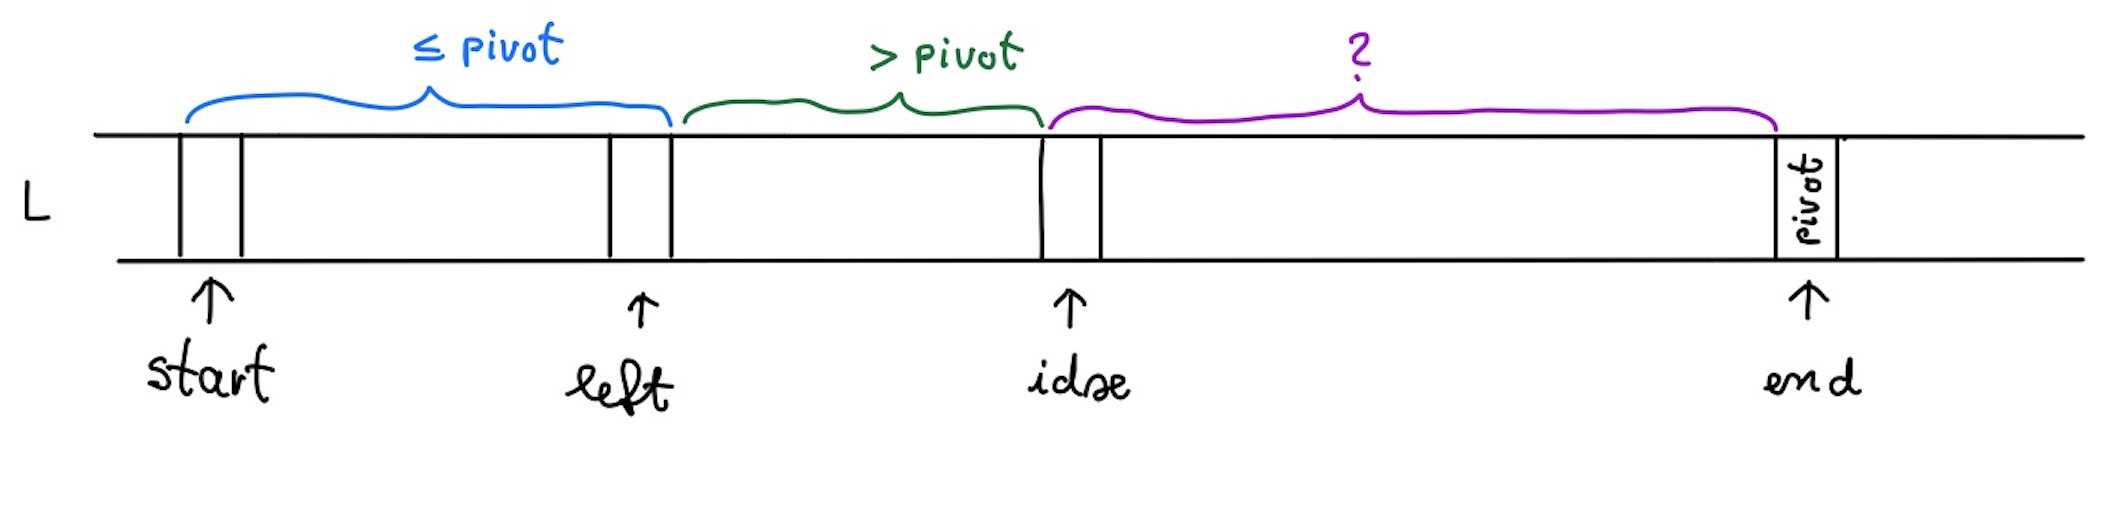
\epsfig{file=Abbildungen/lomuto.png, scale=0.40}} 
  \caption{The invariants of the function \mytt{partition}.}
  \label{fig:lomuto.png}
\end{figure}


      Observe how the invariants (a) and (b) are maintained:
      \begin{enumerate}
      \item Initially, the invariants are true because the corresponding sets are empty.
            At the start of the \mytt{for}-loop we have
            \\[0.2cm]
            \hspace*{1.3cm}
            $\{ \mytt{start}, \cdots, \mytt{left} \} = \{ \mytt{start}, \cdots, \mytt{start} - 1\} = \{\}$
            \\
            and
            \\
            \hspace*{1.3cm}
            $\{ \mytt{left}+1,\cdots,\mytt{idx}-1\} =  \{ \mytt{start},\cdots,\mytt{start}-1\}=\{\}$.
      \item If the element $\mytt{L[idx]}$ is less than the
            pivot element, it need to become part of the subarray $\mytt{L}[\mytt{start}:\mytt{left}+1]$.  In order to
            achieve this, it is placed at the position $\mytt{L}[\mytt{left}+1]$.  The element that has been at
            that position is part of the subarray $\mytt{L}[\mytt{left}+1:\mytt{idx}]$ and therefore,
            most of the times,\footnote{
              It is not always greater than the pivot element
              because the subarray $\mytt{L}[\mytt{left}+1:\mytt{idx}]$ might well be empty.}
            it is greater than the pivot element.  
            Hence we append this element to the end of the subarray
            $\mytt{L}[\mytt{left}+1:\mytt{idx}]$.  After incrementing the index $\mytt{left}$,
            both the placing of the element $\mytt{L[idx]}$ at position $\mytt{left}+1$ and the appending
            of the element $\mytt{L}[\mytt{left}+1]$ to the end of the subarray
            $\mytt{L}[\mytt{left}+1:\mytt{idx}+1]$ is achieved by the statement
            \\[0.2cm]
            \hspace*{1.3cm}
            \mytt{swap(left, idx, L)}.            
      \end{enumerate}
      Once the \mytt{for} loop in line 14 terminates, the call to $\mytt{swap}$ in line 18 moves
      the pivot element into its correct position and returns the index where the pivot element has been
      placed. 
\end{enumerate}


\subsection{Improvements for Quicksort}
There are a number of tricks that can be used to increase the efficiency of \blue{quicksort}.
\begin{enumerate}
\item Instead of taking the first element as the pivot element, use three elements from the list
      $\mytt{L}$ that is to be sorted.  For example, take the first element, the last element, and an
      element from the middle of the list.  Now compare these three elements and take that element as
      a pivot that is the \blue{median} of these elements,  where the \blue{median} \index{median} of three
      elements is defined as the element that lies between the minimum and the maximum of these elements.
      In general, the \blue{median} of a list $L$ of length $2 \cdot n +1$ is defined as the element $x$ such that at
      least $n$ elements of $L$ are less or equal to $x$ and at least $n$ elements are bigger or equal than $x$.
      
      The advantage of this strategy is that the worst case performance is much less likely to occur.  In
      particular,  using this strategy the worst case won't occur for a list that is already
      sorted.
\item If a sublist contains fewer than 10 elements, use \blue{insertion sort} to sort this sublist.

      The paper ``\blue{Engineering a Sort Function}'' by Jon L.~Bentley and M.~Douglas McIlroy
      \cite{bentley:93} describes the previous two improvements.
\item In order to be sure that the average case analysis of \blue{quicksort} holds we can randomly
      \blue{shuffle} the list $L$ that is to be sorted.  This approach is advocated by Sedgewick
      \cite{sedgewick:2011}.  In \textsl{Python} this is quite easy as
      the module \mytt{random} provides a predefined function \mytt{shuffle} that takes a list and shuffles
      it randomly in place.  For example, the code
      \\[0.2cm]
      \hspace*{1.3cm}
      \mytt{L = list(range(10)); random.shuffle(L); print(L)}
      \\[0.2cm]
      might print the result
      \\[0.2cm]
      \hspace*{1.3cm}
      \mytt{[1, 9, 8, 5, 2, 0, 6, 3, 4, 7]}.
\item In 2009, Vladimir Yaroslavskiy introduced \blue{dual pivot quicksort}
      \cite{yaroslavskiy:2009}.\index{dual pivot quicksort}
      His paper can be
      downloaded at the following address:
      \\[0.2cm]
      \hspace*{1.3cm}
      \href{http://codeblab.com/wp-content/uploads/2009/09/DualPivotQuicksort.pdf}{\mytt{http://codeblab.com/wp-content/uploads/2009/09/DualPivotQuicksort.pdf}}
      \\[0.2cm]
      The main idea of Yaroslavskiy is to use two pivot elements $p_1$ and $p_2$.  For example, we can
      define
      \\[0.2cm]
      \hspace*{1.3cm}
      $x := \mytt{L}[0]$, $y := \mytt{L}[-1]$, \quad and then define \quad $p_1 :=\min(x, y)$, $p_2 := \max(x, y)$.
      \\[0.2cm]
      Next, the list $\mytt{L}$ is split into three parts:
      \begin{enumerate}
      \item The first part contains those elements that are less than $p_1$.
      \item The second part contains those elements that are bigger or equal than $p_1$ but less or
            equal than $p_2$.
      \item The third part contains those elements that are bigger than $p_2$.
      \end{enumerate}
      Figure \ref{fig:dual-pivot-quick-sort.stlx} on page \pageref{fig:dual-pivot-quick-sort.stlx}
      shows a simple list-based implementation of \blue{dual pivot quicksort}.

      Various studies have shown that, on average, \blue{dual pivot quicksort} is faster than any other sorting
      algorithm.  For this reason, the version 1.7 of \textsl{Java} uses \blue{dual pivot quicksort}:
      \\[0.2cm]
      \hspace*{0.3cm}
      \href{http://www.docjar.com/html/api/java/util/DualPivotQuicksort.java.html}{http://www.docjar.com/html/api/java/util/DualPivotQuicksort.java.html} 
\end{enumerate}

\begin{figure}[!ht]
\centering
\begin{minted}[ frame         = lines, 
                  framesep      = 0.3cm, 
                  firstnumber   = 1,
                  bgcolor = sepia,
                  numbers       = left,
                  numbersep     = -0.3cm,
                  xleftmargin   = 0.0cm,
                  xrightmargin  = 0.0cm,
                ]{python3}
    def sort(L):
        if len(L) <= 1:
            return L
        x, y, *R   = L
        p1, p2     = min(x, y), max(x,y)
        L1, L2, L3 = partition(p1, p2, R)
        return sort(L1) + [p1] + sort(L2) + [p2] + sort(L3)
    
    def partition(p1, p2, L):
        if L == []:
            return [], [], []
        x, *R      = L
        R1, R2, R3 = partition(p1, p2, R)
        if x < p1:
            return [x] + R1, R2, R3
        if x <= p2:
            return R1, [x] + R2, R3
        else:
            return R1, R2, [x] + R3
\end{minted}
\vspace*{-0.3cm}
\caption{A list based implementation of \blue{dual pivot quicksort}.}
\label{fig:dual-pivot-quick-sort.stlx}
\end{figure}

\exercise
Implement a version of \blue{dual pivot quicksort} that is array-based instead of list-based.
\eoxs


\section{A Lower Bound for the Sorting Problem}
In this section we will show that any sorting algorithm that sorts elements by comparing them must
use at least 
\\[0.2cm]
\hspace*{1.3cm}
 $\Omega\bigl(n \cdot \log_2(n)\bigr)$ 
\\[0.2cm]
comparisons.  The important caveat here is that the sorting algorithm is not permitted to make any assumptions
on the elements of the list $L$ that is to be sorted.  The only operation that is allowed on these
elements is the use of the comparison operator ``\mytt{<}''.  Furthermore, to simplify matters let
us assume that all elements of the list $L$ are distinct.

Let us consider lists of two elements first, i.e.~assume we have
\\[0.2cm]
\hspace*{1.3cm}
$L = [a_1, a_2]$.  
\\[0.2cm]
In order to sort this list, one comparison is sufficient:
\begin{enumerate}
 \item If $a_1 < a_2$, then the list $[a_1, a_2]$ is sorted ascendingly.
 \item If $a_2 < a_1$, then the list $[a_2, a_1]$ is sorted ascendingly.
\end{enumerate}
If the list $L$ that is to be sorted has the form
\\[0.2cm]
\hspace*{1.3cm}
$L = [a_1,a_2,a_3]$,
\\[0.2cm]
then there are 6 possibilities to arrange these elements:
\\[0.2cm]
\hspace*{0.3cm}
$[a_1,a_2,a_3]$, \quad
$[a_1,a_3,a_2]$, \quad
$[a_2,a_1,a_3]$, \quad
$[a_2,a_3,a_1]$, \quad
$[a_3,a_1,a_2]$, \quad
$[a_3,a_2,a_1]$. 
\\[0.2cm]
Therefore, we need at least three comparisons, since with two comparisons we could choose between at most 
four different possibilities.  Next, we generalize this observation.

\begin{Theorem}
Given a list $L$ of $n$ different elements, there are 
\\[0.2cm]
\hspace*{1.3cm}
$\ds n! = 1 \cdot 2 \cdot 3 \cdot {\dots} \cdot (n-1) \cdot n = \prod\limits_{i=1}^n i$ 
\\[0.2cm]
different permutations of $L$. 
\end{Theorem}
\proof The claim is proven by induction on $n$. 
\begin{enumerate}
\item[B.C.:] $n=1$:  

      There is only $1$ way to arrange one element in a list.  As $1! = 1$ the claim is true in this case.
\item[I.S.:] $n \mapsto n+1$:
  
      If we have $n+1$ different elements and want to arrange these elements in a list, then there
      are $n+1$ possibilities for the first element.  In each of these cases the induction
      hypothesis tells us that there are $n!$ ways to arrange the remaining $n$ elements in a list.
      Therefore, all in all there are $(n+1) \cdot n! = (n+1)!$ different arrangements of $n+1$
      elements in a list. \qed
\end{enumerate}
Next, we consider how many different cases can be distinguished if we have $k$ different tests
that only give $\mytt{True}$ or $\mytt{False}$ answers.  Tests of this kind are called \blue{binary tests}.
\begin{enumerate}
\item If we restrict ourselves to binary tests, then one test can only distinguish between two cases.
\item If we have $2$ tests, then we can distinguish between  $2 \cdot 2 = 2^2$ different cases.
\item In general, an easy induction shows that $k$ tests can choose from at most $2^k$ different cases.
\end{enumerate}
The last claim can also be argued as follows:  If the results of the tests are represented as
$0$ and $1$, then $k$ binary tests correspond to a binary string of length
$k$.  However, binary strings of length $k$ can be used to code the numbers from $0$ up to
$2^{k}-1$.  We have
\\[0.2cm]
\hspace*{1.3cm}
$\textsl{card}\bigl(\{0,1,2,\cdots, 2^k-1\}\bigr) = 2^k$.
\\[0.2cm]
Hence there are $2^k$ binary strings of length $k$.  

If we have a list of $n$ different elements, then there are $n!$ different permutations of these
elements.  In order to figure out which of these $n!$ different permutations is given we have to
perform $k$ comparisons, where we must have
\\[0.2cm]
\hspace*{1.3cm}
$2^k \geq n!$.
\\[0.2cm]
This immediately implies
\\[0.2cm]
\hspace*{1.3cm}
$k \geq \log_2(n!)$.
\\[0.2cm]
In order to proceed, we need a lower bound for the expression $\log_2(n!)$.
First, we have
\\[0.2cm]
\hspace*{1.3cm}
$\ds \log_2(n!) = \log_2\left(\prod\limits_{i=1}^n i\right) = \sum\limits_{i=1}^n \log_2(i)$
\\[0.2cm]
The crucial idea is to interpret this sum as an upper \href{https://en.wikipedia.org/wiki/Riemann_sum}{Riemann sum}
of the integral
\\[0.2cm]
\hspace*{1.3cm}
$\ds\int_1^n\log_2(x)\, \mathrm{d}x$
\\[0.2cm]
as is shown in Figure \ref{fig:riemann-sum.pdf}\footnote{
  I have created this figure using the highly recommended tool \href{https://www.geogebra.org/m/h4P4cjsT}{geogebra}.
}.

\begin{figure}[!ht]
  \centering
  \framebox{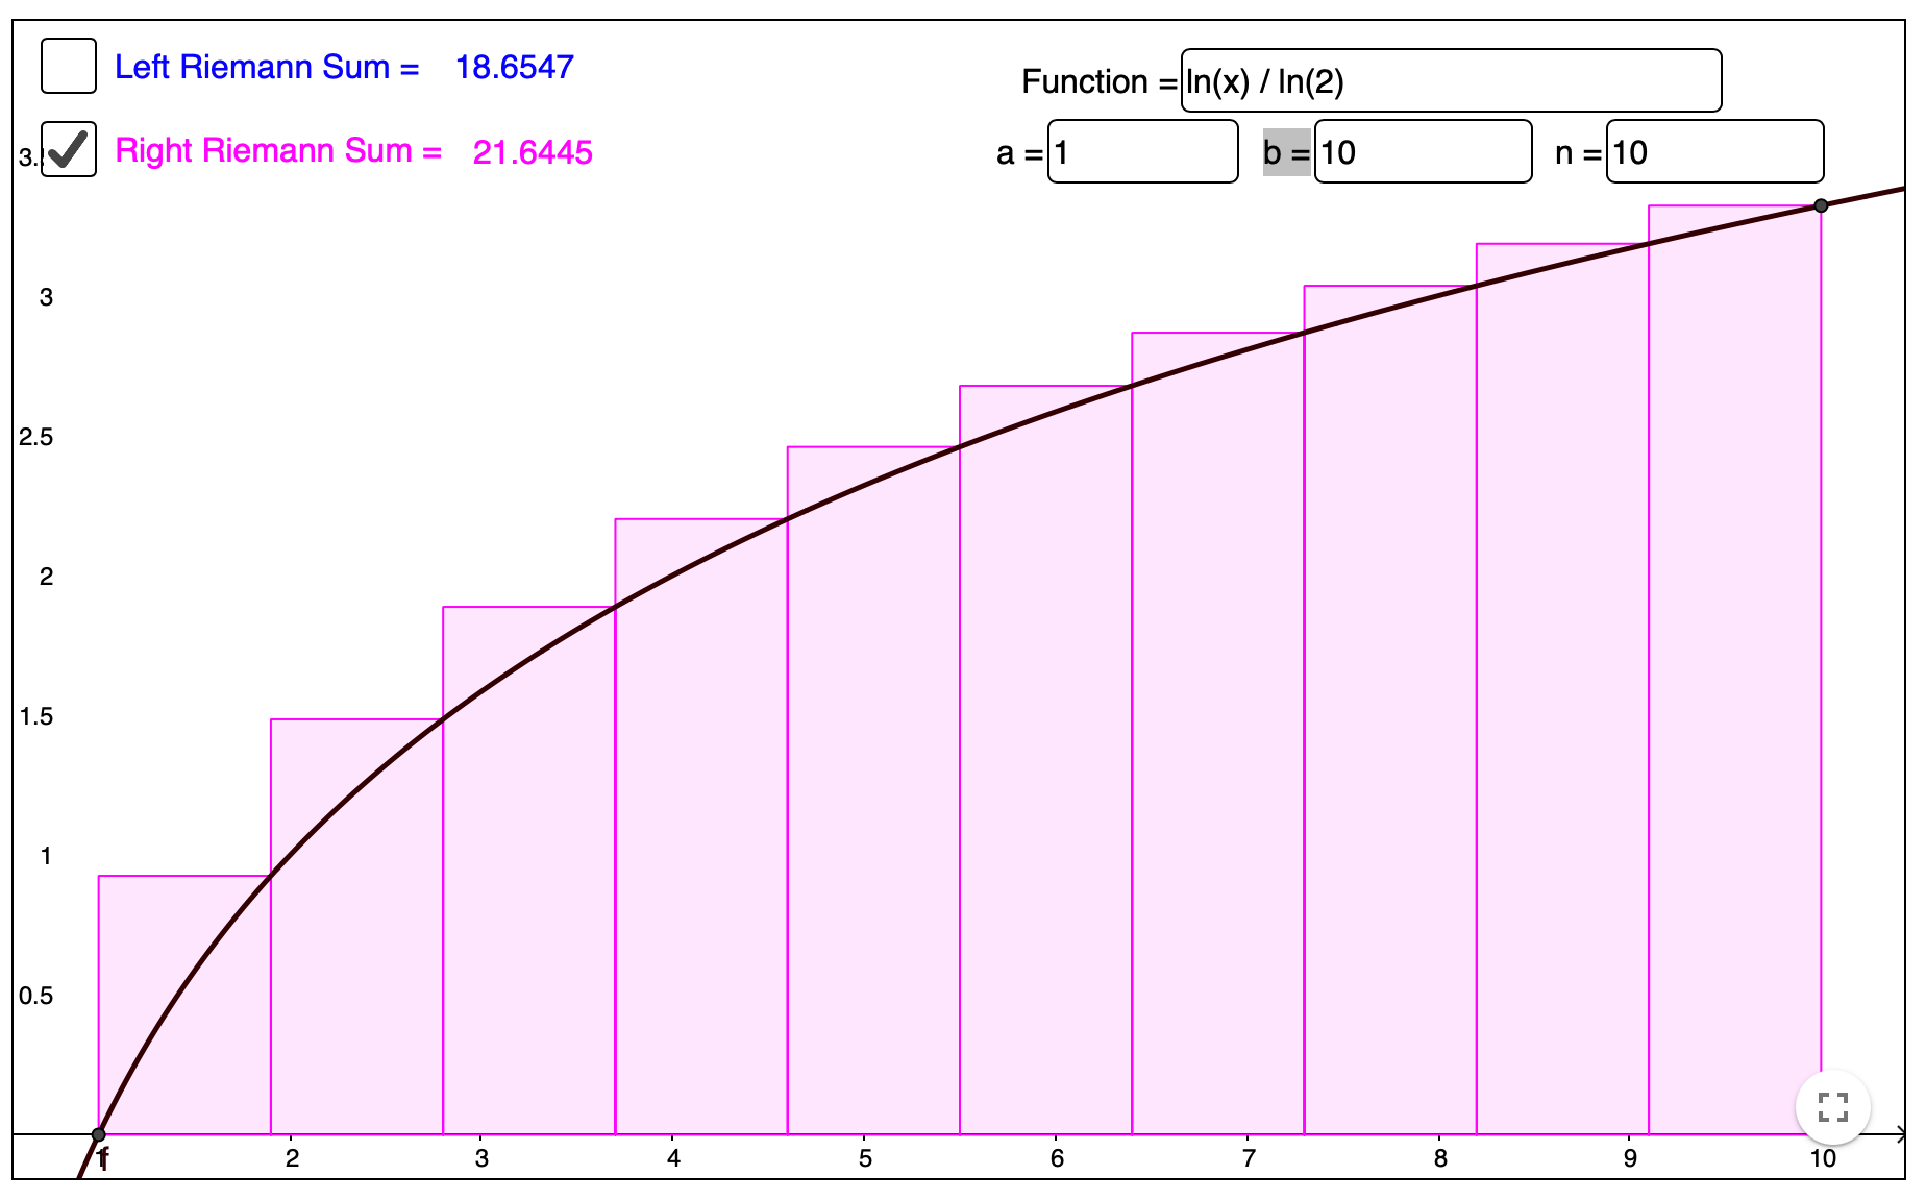
\epsfig{file=Abbildungen/riemann-sum.pdf, scale=0.45}} 
  \caption{The upper sum for the integral $\ds\int\limits_{1}^{10}\log_2(x) \,\mathrm{d}x$.}
  \label{fig:riemann-sum.pdf}
\end{figure}

Therefore we have the following chain of inequations:
\\[0.2cm]
\hspace*{1.3cm}
$
\begin{array}[t]{lcl}
  k & \geq & \ds\log_2(n!) \\[0.2cm]
    & =    & \ds\sum\limits_{i=1}^n \log_2(i) \\[0.5cm]
    & \geq & \ds\int\limits_{1}^n \log_2(x)\, \mathrm{d}x \\[0.2cm]
    & =    & \ds\frac{1}{\,\ln(2)\,} \cdot \int\limits_{1}^n \ln(x)\, \mathrm{d}x  \\[0.2cm]
    & =    & \ds\frac{1}{\,\ln(2)\,} \cdot \bigl[x \cdot \ln(x) - x \bigr]_{1}^n   \\[0.4cm]
    & =    & \ds\frac{1}{\,\ln(2)\,} \cdot \bigl(n \cdot \ln(n) - n + 1\bigr)     \\[0.2cm]
    & =    & \ds n \cdot \log_2(n) - \frac{\,n-1\,}{\,\ln(2)\,}                       
\end{array}
$ 
\\[0.2cm]
This show that
\\[0.2cm]
\hspace*{1.3cm}
$k \geq n \cdot \ds\log_2(n) - \frac{\,n-1\,}{\,\ln(2)\,}$.
\\[0.2cm]
As \blue{merge sort} is able to sort a list of length $n$ using only $n \cdot \log_2(n)$ comparisons
we have shown that this algorithm is optimal with respect to the number of comparisons within a linear bound of
size $(n-1)/\ln(2)$.




\section{Counting Sort}
\index{counting sort}
In the last section of this chapter we introduce a sorting algorithm that has only a \blue{linear} complexity.
According to the result of the previous section this algorithm can not work by comparing the elements of the
list that is to be sorted.  This algorithm only works if the elements of the list that is to be sorted are
natural numbers of a fixed size.  The algorithm is called
\href{https://en.wikipedia.org/wiki/Counting_sort}{counting sort}. We 
explain this algorithm via an example.  Table \ref{tab:marks} on page \pageref{tab:marks} shows a table showing
students and their grades.  As it stands, the names of the students are ordered alphabetically.  However, the
teacher would like to sort the list of students according to their grades.  Within a group of students that
have achieved the same grade, the students should still be ordered alphabetically.  Table
\ref{tab:marks-sorted} on page \pageref{tab:marks-sorted} shows the table that has been sorted accordingly.

\begin{table}[!ht]
  \centering
  \begin{tabular}{|l|c|}
    \hline
    Student   & Grade \\
    \hline
    \hline
    Alexander & 4 \\
    \hline
    Benjamin  & 2 \\
    \hline
    Daniel    & 3 \\
    \hline
    David     & 3 \\
    \hline
    Elijah    & 2 \\
    \hline
    Gabriel   & 1 \\
    \hline
    Henry     & 2 \\
    \hline
    Jacob     & 5 \\
    \hline
    James     & 3 \\
    \hline
    Joseph    & 2 \\
    \hline
    Liam      & 2 \\
    \hline
    Logan     & 3 \\
    \hline
    Lucas     & 1 \\
    \hline
    Mason     & 2 \\
    \hline
    Matthew   & 5 \\
    \hline
    Michael   & 3 \\
    \hline
    Noah      & 4 \\
    \hline
    Oliver    & 2 \\
    \hline
    Owen      & 4 \\
    \hline
    Samuel    & 3 \\
    \hline
    Sebastian & 2 \\
    \hline
    William   & 1 \\
    \hline
  \end{tabular}
  \caption{Students and their grades, sorted alphabetically.}
  \label{tab:marks}
\end{table}

\begin{table}[!ht]
  \centering
  \begin{tabular}{|l|c|}
    \hline
    Student   & Grade \\
    \hline
    \hline
    Gabriel   & 1 \\
    \hline
    Lucas     & 1 \\
    \hline
    William   & 1 \\
    \hline
    Benjamin  & 2 \\
    \hline
    Elijah    & 2 \\
    \hline
    Henry     & 2 \\
    \hline
    Joseph    & 2 \\
    \hline
    Liam      & 2 \\
    \hline
    Mason     & 2 \\
    \hline
    Oliver    & 2 \\
    \hline
    Sebastian & 2 \\
    \hline
    Daniel    & 3 \\
    \hline
    David     & 3 \\
    \hline
    James     & 3 \\
    \hline
    Logan     & 3 \\
    \hline
    Michael   & 3 \\
    \hline
    Samuel    & 3 \\
    \hline
    Alexander & 4 \\
    \hline
    Noah      & 4 \\
    \hline
    Owen      & 4 \\
    \hline
    Jacob     & 5 \\
    \hline
    Matthew   & 5 \\
    \hline
  \end{tabular}
  \caption{Students and their grades, sorted with respect to the grade.}
  \label{tab:marks-sorted}
\end{table}
We proceed to describe an algorithm that is capable of transforming Table \ref{tab:marks} into Table
\ref{tab:marks-sorted}.  This algorithm works in three stages.
\begin{enumerate}
\item The first stage is the \blue{counting stage}.  In this stage we count the number of students
      that have a specific grades.  In the example from Table \ref{tab:marks} we find the following:
      \begin{enumerate}[(a)]
      \item 3 students have grade 1.
      \item 8 students have grade 2.
      \item 6 students have grade 3.
      \item 3 students have grade 4.
      \item 2 students have grade 5.
      \end{enumerate}
\item The second stage is the \blue{indexing stage}.  In this stage our goal is compute the indices of the
      sublists containing the different grades.  For example, since there are 3 students with a grade of $1$
      and $1$ is the smallest grade, we know that the students with grade $1$ will be found in the sublist
      $\mytt{L[0:3]}$.  Similarly, as there are $8$ students that have a grade of $2$ and $3 + 8 = 11$,
      the sublist $\mytt{L[3:11]}$ will contain the students with grade $2$.
      All in all, we have the following:
      \begin{enumerate}[(a)]
      \item The sublist $\mytt{L[0:3]}$ contains the students with grade 1.
      \item The sublist $\mytt{L[3:11]}$ contains the students with grade 2.
      \item The sublist $\mytt{L[11:17]}$ contains the students with grade 3.
      \item The sublist $\mytt{L[17:20]}$ contains the students with grade 4.
      \item The sublist $\mytt{L[20:22]}$ contains the losers.
      \end{enumerate}
      The indexing stage computes the \blue{starting indices} of these sublists.
      Of course,  the first sublist has to start at the index $0$.  Since there are 3 students with a grade of 1,
      the second sublist starts at the index $0 + 3 = 3$.  Since there are 8 students with a grade of 2, the third
      sublist starts at the index $0 + 3 + 8 = 11$.  In general, if the sublist for the students with grade $g$
      starts at index $i_g$ and there are $n_g$ students that have achieved the grade $g$, then the sublist for the
      students with grade $g+1$ starts at index $i_{g+1}$ where
      \\[0.2cm]
      \hspace*{1.3cm}
      $\ds i_{g+1} = i_g + n_g$.
\item The \blue{distribution stage} iterates over the list of students and inserts them into the sublists
      corresponding to the grades of the students.
\end{enumerate}
Figure \ref{fig:counting-sort.stlx} on page \pageref{fig:counting-sort.stlx} shows an implementation of
counting sort.  We proceed to discuss this algorithm line by line.

\begin{figure}[!ht]
\centering
\begin{minted}[ frame         = lines, 
                  framesep      = 0.3cm, 
                  firstnumber   = 1,
                  bgcolor = sepia,
                  numbers       = left,
                  numbersep     = -0.2cm,
                  xleftmargin   = 0.8cm,
                  xrightmargin  = 0.8cm,
                ]{python3}
    def countingSort(Students):
        maxGrade =    255
        Counts   =    [0] * (maxGrade+1)
        Index    = [None] * (maxGrade+1)
        Sorted   = [None] * len(Students)
        # Phase 1: Counting
        for _name, grade in Students:
            Counts[grade] += 1
        # Phase 2: Indexing
        Index[0] = 0
        for grade in range(maxGrade):
            Index[grade+1] = Index[grade] + Counts[grade]
        # Phase 3: Distribution
        for name, grade in Students:
            idx           = Index[grade]
            Sorted[idx]   = (name, grade)
            Index[grade] += 1
        return Sorted
\end{minted}
\vspace*{-0.3cm}
\caption{An implementation of \blue{counting sort}.}
\label{fig:counting-sort.stlx}
\end{figure}

\begin{enumerate}
\item The procedure \mytt{countingSort} receives one argument.  The list $\mytt{Students}$
      is a list of pairs of the form $\mytt{(name, grade)}$ where
      \begin{enumerate}
      \item \mytt{name}  is the name of a student, while
      \item \mytt{grade} is the grade that this student has achieved.
      \end{enumerate}
      The list $\mytt{Students}$ is sorted alphabetically w.r.t.~the names of the students.
      The purpose of the function \mytt{countingSort} is to sort this list according to their grades.
      Sublists of students with the same grade should still be sorted alphabetically.
\item In order for our function to generalize to arbitrary numbers we will assume that all grades are elements
      of the set $\{0,\cdots,255\}$.  Therefore we define $\mytt{maxGrade}$ as $255$.
      Of course, in the example discussed so far we know that the largest
      grade is $5$.  However, we will use the function $\mytt{countingSort}$ later as an auxiliary function
      when implementing \blue{radix sort}.  Then the grades will be bytes and hence be natural numbers less
      or equal than $255$.
\item Next, we initialize the auxiliary array \mytt{Count} to be an array of length $\mytt{maxGrade}+1$.
      Later, for a grade $g$ the number $\mytt{Counts}[g]$ will contain the number of students that have
      attained the grade $g$.  Initially, all entries of the array \mytt{Count} are set to $0$.
\item After the indexing stage, the array \mytt{Index} will contain the start indices of the different sublists.
      For a grade $g$, $\mytt{Index}[g]$ is the first index of the sublist containing those students that
      have achieved the grade $g$.
\item The list \mytt{Sorted} is the list that will be returned as the result.
      This list will contain pairs of the form \mytt{(name, grade)} where \mytt{name} is the name of a student
      and \mytt{grade} is her grade.
\item The \mytt{for}-loop in line 7-8 performs the \blue{counting stage}.  We iterate over all grades
      in the list \mytt{Students} and increment the counter $\mytt{Counts}[\mytt{grade}]$ that is associated with the given grade.
\item Next, the index for the start of the sublist containing those students that have achieved the grade $0$
      is initialized as $0$ in line 10. 
\item Then, the \mytt{for}-loop in line 11-12 performs the \blue{indexing stage}. As the number
      $\mytt{Index}[\mytt{grade}]$ is the index of the start of the sublist for those students that have
      achieved the grade  $\mytt{grade}$ and the number of these
      students is $\mytt{Counts}[\mytt{grade}]$, the sublist of the students with grade $\mytt{grade}+1$
      has to start at index 
      \\[0.2cm]
      \hspace*{1.3cm}
      $\mytt{Index}[\mytt{grade}] + \mytt{Counts}[\mytt{grade}]$.
\item Finally, the \mytt{for}-loop in line 14-17 performs the \blue{distribution stage}.
      \begin{enumerate}
      \item The \mytt{for}-loop iterates over all students. 
      \item We need to find where to put a student with grade \mytt{grade}.
            $\mytt{Index}[\mytt{grade}]$ gives us the \mytt{index} of the next free entry in the
            result list \mytt{Sorted} corresponding for this grade.
      \item In line 16 the students name and her grade are stored in the result lists \mytt{Sorted}
            at the index $\mytt{idx}$.
      \item Finally, we need to increment the index stored at $\mytt{Index}[\mytt{grade}]$ since we have
            just used this index and therefore the next student with the same grade needs to be
            stored at the subsequent location.  This is done in line 17.
      \end{enumerate}
\end{enumerate}
If the list \mytt{Students} has a length of $n$, then it is easy to
see that counting sort has the complexity $\Oh(n)$.  The first \mytt{for}-loop iterates over the list \mytt{Students} so
its body is executed $n$ times.  The second for loop iterates 255 times and the last \mytt{for}-loop again
iterates $n$ times.  Hence, counting sort is a \blue{linear sorting algorithm}.  Note that we do not compare grades in
order to sort them.

Another important fact is that counting sort is \blue{stable}\index{stable}: In the resulting list, the sublists
corresponding to the different grades are still sorted alphabetically.  This is so because these sublists are
filled by iterating over the original list that is sorted alphabetically.  If two students $x$ and $y$ have the
same grade $g$ but the name of $x$ is alphabetically before the name of $y$, then $x$ will be inserted into the
sublist corresponding to grade $g$ before $y$ and hence these sublists are still ordered alphabetically.  This property
is crucial for the development of our next sorting algorithm \blue{radix sort}.

\section{Radix Sort}
\index{radix sort}
The importance of the previous sorting algorithm, \blue{counting sort}, stems from the fact that it is part of the
implementation of \href{https://en.wikipedia.org/wiki/Radix_sort}{radix sort}. \index{radix sort}
\blue{Radix sort} was used as early as 1887 in 
\href{https://en.wikipedia.org/wiki/Tabulating_machine}{tabulating machines} constructed by
\href{https://en.wikipedia.org/wiki/Herman_Hollerith}{Hermann Hollerith}.  \index{Hollerith, Herman} He was the founder of
the \blue{Tabulating Machine Company} that later became \href{https://en.wikipedia.org/wiki/IBM}{\textsc{Ibm}}.
To understand radix sort, suppose we want to implement an algorithm that sorts a large number of 32 bit
unsigned integers.  The easiest way to do this would be to use counting sort:
The main idea of radix sort is to split the
32 bit numbers into four chunks of 8 bits each and to use each of these four chunks as a grade.  To formulate this
mathematically, a 32 bit unsigned integer $x$ is defined via its four bytes $b_1$, $\cdots$, $b_4$ as follows:
\\[0.2cm]
\hspace*{1.3cm}
$\ds x = b_4 \cdot 256^{3} + b_3 \cdot 256^{2} + b_2 \cdot 256^{1} + b_1$.
\\[0.2cm]
Note that we have numbered the bytes starting from the the least significant byte.
Then, radix sort works as follows:
\begin{enumerate}
\item Sort the numbers by interpreting the byte $b_1$ as a grade.
\item Take the numbers that have been sorted by the byte $b_1$ and sort them according to the byte $b_2$ next.
      Since counting sort is \blue{stable}, numbers which happen to have the same byte $b_2$ will still be
      sorted with respect to the byte $b_1$.  Hence, after the sorting with respect to the byte $b_2$ is
      complete, in effect the numbers will then be sorted according to both $b_2$ and $b_1$.
\item Next, use counting sort to sort the numbers with respect to the byte $b_3$.
\item Finally, use counting sort to sort the numbers with respect to the byte $b_4$.  By the stability of
      counting sort, the numbers are now sorted with respect to all of their byte, where $b_4$ is the most
      significant byte and $b_1$ is the least significant byte. Hence, the numbers are sorted. 
\end{enumerate}


\begin{figure}[!ht]
\centering
\begin{minted}[ frame         = lines, 
                  framesep      = 0.3cm, 
                  firstnumber   = 1,
                  bgcolor = sepia,
                  numbers       = left,
                  numbersep     = -0.2cm,
                  xleftmargin   = 0.8cm,
                  xrightmargin  = 0.8cm,
                  ]{python3}
    def extractByte(n, k):
        return n >> (8 * (k-1)) & 0b11111111
    
    def radixSort(L):
        L = [(n, 0) for n in L]
        for k in range(1, 4+1):
            L = [(n, extractByte(n, k)) for (n, _) in L]
            L = countingSort(L)
        return [n for (n, _) in L]    
\end{minted}
\vspace*{-0.3cm}
\caption{An implementation of \blue{radix sort} for sorting unsigned 32 integers.}
\label{fig:radix-sort.stlx}
\end{figure}
Figure \ref{fig:radix-sort.stlx} on page \pageref{fig:radix-sort.stlx} shows an implementation of radix
sort that implements this idea.
\begin{enumerate}
\item The function \mytt{extractByte} is called with two arguments:
      \begin{enumerate}[(a)]
      \item $n$ is supposed to be an unsigned 32 bit number.  Hence $n$ is a integer satisfying $0 \leq n < 2^{32}$.
      \item $k$ is the index of the byte that is to be extracted.  It is supposed that the least significant
            byte has the index $1$.
      \end{enumerate}
      Hence, $\mytt{extractByte}(n, k)$ extracts the $k$-th byte of the number $n$.

      \mytt{extractByte} works by shifting the number $x$ by $(k-1) \cdot 8$ bits to the right using the shift
      operator ``\mytt{>>}''.  This shift removes all bytes with index less than $k$. Then, the least significant
      byte of the remaining number is extracted using the  \blue{bitwise and operator} ``\mytt{\&}'' with the
      mask $255$.  Note that $255$ is written as $11111111_2$ in binary and hence can be used to extract the
      eight least significant bits of a number. 
\item \mytt{radixSort} takes a list of unsigned 32 bit integers $L$ as its arguments.
\item This list is extended to a list of pairs where the first component of each pair is the number.      
\item Then \mytt{radixSort} iterates over the four bytes of the numbers of the list $L$ starting with the
      least significant byte.
\item In line 7 the $k^\mathrm{th}$ byte of the numbers of $L$ is written into the second component
      of the pairs stored in the list.      
\item With respect to \mytt{countingSort},  the elements of the list given to \mytt{countingSort} as its
      first argument are 
      arbitrary objects.  Therefore, it does not matter whether the first argument to the function
      \mytt{countingSort} is a list of strings interpreted as student names or a list of numbers.
      Therefore in line 8 this list
      is sorted with respect to the $k^\mathrm{th}$ byte. 
\item When $L$ is returned, this list is sorted with respect to all of the four bytes making up its numbers and
      hence, it is sorted.
\end{enumerate}

\section{Application: Handwritten Digit Recognition}
\index{digit recognition}
In the last section of this chapter we discuss an application of sorting:
\blue{recognizing handwritten digits}.\index{handwritten digit recognition}
We will use a \blue{training set} of $50,000$ handwritten digits. Figure \ref{fig:digits.pdf} shows the first 24
images of these handwritten digits.  These images are given as grey scale images of $28 \times 28$ pixels.
Each pixel $p$ is a floating point number satisfying $0 \leq p \leq 1$. If $p = 1.0$, the pixel is completely
black, while $p = 0.0$ if the pixel is white.  Furthermore, for each of these images we also have been given a
\blue{label} $d \in \{0,1,2,\cdots,9\}$, which specifies the digit that is represented in the image.  Besides the training set 
there is also a \blue{test set} of $10,000$ of handwritten images.  Our task is to \blue{classify} the images
of this test set as digits, i.e.~for each image of the test set we want to recognize the digit that is depicted.


\begin{figure}[!ht]
  \centering
  \framebox{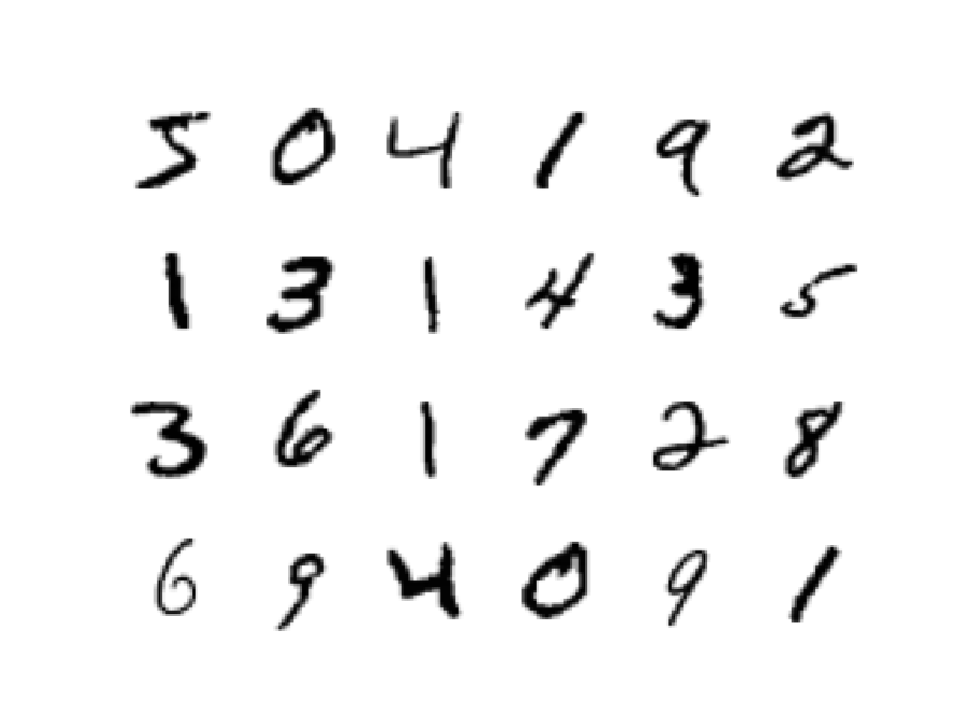
\epsfig{file=Abbildungen/digits.pdf, scale=0.60}} 
  \caption{The first 24 digits of our dataset.}
  \label{fig:digits.pdf}
\end{figure}

\subsection{The $k$-Nearest Neighbour Algorithm}
We will use the \href{https://en.wikipedia.org/wiki/K-nearest_neighbors_algorithm}{$k$-nearest neighbours algorithm} 
\index{$k$-nearest neighbours algorithm}
to solve this task.  Given an image $x$ that is to be classified as a digit, we look at those images in the
training set that are somehow \blue{close} to $x$.  If these images are all labelled with the same digit $d$,
we conclude that $x$ shows the digit $d$.  In order to implement this algorithm, we have to specify what it
means for an image $\mathbf{x}$ to be close to another image $\mathbf{y}$.  As the images have a size of $28 \times 28 = 784$
pixels, they can be viewed as $784$-dimensional vectors.  We can compute the \blue{Euclidean distance}
$d(\mathbf{x}, \mathbf{y})$ between $\mathbf{x}$ and $\mathbf{y}$ using the formula
\\[0.2cm]
\hspace*{1.3cm}
$\ds d(\mathbf{x}, \mathbf{y}) := \sqrt{\sum\limits_{i=1}^n (x_i - y_i)^2\;}$.
\\[0.2cm]
This formula is a generalization of the distance between two points $(x_1, x_2)$ and $(y_1, y_2)$ in the the
plane $\mathbb{R}^2$, which, according to the \href{https://en.wikipedia.org/wiki/Pythagorean_theorem}{Pythagorean theorem}, is given as 
\\[0.2cm]
\hspace*{1.3cm}
$\sqrt{(x_1 - y_1)^2 + (x_2 - y_2)^2\;}$.
\\[0.2cm]
Given an image $\mathbf{y}$ that needs to be classified and a training set of $n$ labelled images, the $k$-nearest
neighbours algorithm works as follows: 
\begin{enumerate}[(a)]
\item For every image $\mathbf{x}$ in the training set compute the Euclidean distance $d(\mathbf{x},
  \mathbf{y})$ between $\mathbf{x}$ and $\mathbf{y}$.
\item \blue{Sort} the images in the training set according to their distance to $\mathbf{y}$.
\item Pick those $k$ images that have the smallest distances to $\mathbf{y}$.
      These $k$ images are called the \blue{$k$ nearest neighbours}.
\item Among the $k$ nearest neighbours, pick the label that occurs most frequently.
      
      For example, if $k=7$ and $3$ of the $7$ nearest neighbours are labelled as the digit $3$, while $2$ are
      labelled as the digit $2$ and $2$ are labelled as the digit $1$, then we conclude that the image
      $\mathbf{y}$ shows the digit $3$. 
\end{enumerate}

\begin{figure}[!ht]
\centering
\begin{minted}[ frame         = lines, 
                 framesep      = 0.3cm, 
                 firstnumber   = 1,
                 bgcolor       = sepia,
                 numbers       = left,
                 numbersep     = -0.3cm,
                 xleftmargin   = 0.0cm,
                 xrightmargin  = 0.0cm,
               ]{python3}
    import gzip
    import pickle
    import numpy as np

    def load_data():
        with gzip.open('mnist.pkl.gz', 'rb') as f:
            train, _, test = pickle.load(f, encoding="latin1")
        return (train[0], test[0], train[1], test[1])
        
    X_train, X_test, Y_train, Y_test = load_data()
        
    def distance(x, y):
        return np.sqrt(np.sum((x - y)**2))
    
    def maxCount(L):
        Frequencies         = {}    # number of occurrences 
        most_frequent       = L[0]  # most frequent digit so far
        most_frequent_count = 1     
        for d in L:
            if d in Frequencies:
                Frequencies[d] += 1
            else:
                Frequencies[d]  = 1
            if Frequencies[d] > most_frequent_count:
                most_frequent       = d
                most_frequent_count = Frequencies[d]
        return most_frequent, most_frequent_count / len(L)
    
    def digit(x, k):
        n          = X_train.shape[0]  # number of all training images
        Distances  = [(distance(X_train[i,:], x), i) for i in range(n)]
        Neighbours = [Y_train[i] for _, i in sorted(Distances)]
        return maxCount(Neighbours[:k])

    digit(X_test[0,:], 13)
\end{minted}
\vspace*{-0.3cm}
\caption{The $k$-nearest neighbours algorithm for digit recognition.}
\label{fig:Digit-Recognition.ipynb}
\end{figure}

\noindent
Figure \ref{fig:Digit-Recognition.ipynb} on page \pageref{fig:Digit-Recognition.ipynb} shows a program that can
be used to recognize a handwritten digit.
\begin{enumerate}
\item The images of the handwritten digits are stored in the file \mytt{mnist.pkl.gz}.  This file is compressed
      using \mytt{gzip} and the images have been \blue{pickled} using the module
      \mytt{pickle}\index{pickle}.  The module
      \mytt{pickle} supports the reading and writing of \textsl{Python} data structures and is therefore
      used to make data \blue{persistent}, i.e.~to store the data structures of a program in a file system.
      The counterpart of the function \mytt{load} is the function \mytt{dump}.

      In order to read the images of the handwritten digits, we therefore have to import the modules
      \mytt{gzip} and \mytt{pickle}.  The module \mytt{numpy} is needed as these images are stored as
      \mytt{numpy} \blue{arrays}.  
\item The function $\mytt{load\_data}()$ returns a tuple of the form
      \\[0.2cm]
      \hspace*{1.3cm}
      $ \ds (\mytt{X\_train}, \mytt{X\_test}, \mytt{Y\_train}, \mytt{Y\_test}) $
      \\[0.2cm]
      where 
      \begin{enumerate}[(a)]
      \item $\mytt{X\_train}$ is a matrix storing the 50,000 training images of handwritten digits.
            For each $i \in \{0,\cdots,49\,999\}$ the row $\mytt{X\_train}[i, :]$ is an array of size $784$ storing a single image.
      \item $\mytt{X\_test}$ is a matrix containing 10,000 images of handwritten digits that we will use to
            test our implementation.
      \item $\mytt{Y\_train}$ is an array of size 50,000. For each $i \in \{0,\cdots,49\,999\}$ the number $\mytt{Y\_train}[i]$
            specifies the digit shown in the $i$th training image.
      \item $\mytt{Y\_test}$ is an array of size 10,000. For each $i \in \{0,\cdots,9\,999\}$ the number $\mytt{Y\_test}[i]$
            specifies the digit shown in the $i^{\mathrm{th}}$ test image.
      \end{enumerate}
      The function \mytt{open} from the module \mytt{gzip} opens the specified file and automatically
      decompresses it.  In the file \mytt{mnist.pkl.gz} the data is stored as a triple of pairs.
      For our purposes, we only need the first and the last component of this triple.  Each of these components
      is a pair of the form $(\textsl{data}, \textsl{label})$, where \textsl{data} is an array of images and
      \textsl{labels} is an array specifying the digits represented in these images.
      The function \mytt{load\_data} extracts the data stored in these pairs.
\item The function $\mytt{distance}(x, y)$ computes the Euclidean distance between the images $x$ and $y$.
      Given a vector $x$, the expression $x \mytt{**} 2$ computes a vector containing the squares of the
      components of $x$.  These squares can then be summed using the \mytt{numpy} function \mytt{sum}.
\item Given a list $L$ of digits, the function $\mytt{maxCounts}(L)$ returns a pair $(d, p)$ where $d$ is the digit that occurs most frequently in $L$
      and $p$ is the fraction of occurrences of $d$ in $L$.  For example, we have
      \\[0.2cm]
      \hspace*{1.3cm}
      $\mytt{maxCounts}([5,2,3,5,2,5,6,5,7,8]) = (5, 0.4)$
      \\[0.2cm]
      because the digit $5$ is the most frequent digit in the list $[5,2,3,5,2,5,6,5,7,8]$ and $40$\%
      of the digits in this list are fives.  In detail, the function \mytt{maxCounts} works as follows:
      \begin{enumerate}[(a)]
      \item \mytt{Frequencies} is a dictionary that specifies how often a digit $d$ occurs in the list $L$.
      \item \mytt{most\_frequent} is the digit that so far is known to be the most frequent digit in $L$.
            Initially, this is assumed to be the first digit.  As we iterate over the list $L$, this variable
            is updated.
      \item \mytt{most\_frequent\_count} is the number of occurrences of the digit \mytt{most\_frequent}.
      \item As we iterate over the digits in $L$ we update their frequencies.  If we encounter a digit that is
            more common than the digit stored in the variable \mytt{most\_frequent} we update this variable
            and the associated value \mytt{most\_frequent\_count}.
      \end{enumerate}
\item Given an image of a digit stored in the vector $\mathbf{x}$ and a number of neighbours $k$, the function
      $\mytt{digit}(\mathbf{x}, k)$ computes those $k$ images in the training set \mytt{X\_train} that are
      \blue{closest} to the image $\mathbf{x}$, where \blue{closeness} of images is defined in terms of the
      \blue{Euclidean distance} of the vectors that store these images.  From these $k$ closest images of the training
      set the function chooses the digit that occurs most frequently.  It returns a pair $(d, p)$ where $d$
      is the digit that is most frequently occurring in the list of $k$ neighbours and $p$ is the percentage
      of images in the $k$ neighbours of $\mathbf{x}$ that show the digit $d$.  The implementation works as follows:
      \begin{enumerate}[(a)]
      \item \mytt{n} is the number of training examples.  In our case, $n = 50,000$.
      \item \mytt{Distances} is a list of pairs of the form $(d, i)$, where $d$ is the distance
            of the $i$-th image in the training set from the given image $x$.
      \item These pairs are \blue{sorted} with respect to their distance and the labels corresponding to the
            images are computed.  Therefore, \mytt{Neighbours} is a list of the labels of all $50,000$
            training images sorted according to their distance to the given image $x$.
      \item Finally, the function \mytt{maxCounts} takes the $k$ closest images and computes the digit that
            is most frequently occurring.
      \end{enumerate}
\item The last line shows how the function \mytt{digit} can be used to classify the first image from the test
      set using the 13 closest neighbours. 
\end{enumerate}
\pagebreak

\exercise
In the program shown in Figure \ref{fig:Digit-Recognition.ipynb} on page \pageref{fig:Digit-Recognition.ipynb}
we have sorted the list \mytt{Distances} in line 32.  The only reason to do this was to be able to find the $k$ smallest
distances in this list.  As $k$ is a small number and the list \mytt{Distances} is rather large, this seems wasteful.
\begin{enumerate}[(a)]
\item Devise an algorithm Quickselect that selects the $k$ smallest elements from a list $L$.

      \hint
      Try to adapt the algorithm Quicksort so that instead of sorting the list it finds the $k$ smallest elements.      
\item Analyse the average complexity of your algorithm.

      \hint
      The recurrence equation resulting from an efficient implementation of Quickselect is quite complicated.
      Instead of solving this recurrence equation it is sufficient if you are able to prove by induction on the
      length $n$ of the list $L$ that your algorithm uses at most $4 \cdot n$ comparisons in order to compute
      the $k$ smallest elements.
      \eox
\end{enumerate}   
\pagebreak

\section{Check Your Understanding}
If you are able to answer the questions below confidently, then you can assume that you have mastered the concepts
introduced in this chapter.
\begin{enumerate}
\item How have we defined the concept of a \blue{linear order}?
\item What type of order do we need if we have to sort a list?
\item Describe the algorithm \blue{insertion sort} on an abstract mathematical level.
\item What is the complexity of \blue{insertion sort}?
\item Is there a case where \blue{insertion sort}  has only a linear complexity?
\item Describe the algorithm \blue{selection sort} on an abstract mathematical level.
\item What is the complexity of \blue{selection sort}?
\item Compare the complexity of \blue{selection sort} with the complexity of \blue{insertion sort}.
\item Describe the algorithm \blue{merge sort} on an abstract mathematical level.
\item Describe an array-based, non-recursive implementation of \blue{merge sort}.
\item Describe the algorithm \blue{quicksort} on an abstract mathematical level.
\item Describe an array-based implementation of \blue{quicksort}.
\item Compare the complexity of \blue{merge sort} with the complexity of \blue{quicksort}.
\item Compare the memory requierements of \blue{merge sort} and \blue{quicksort}.
\item Describe \blue{dual pivot quicksort}.
\item In which case is \blue{dual pivot quicksort} much faster than \blue{quicksort}?
\item How does \blue{counting sort} work?
\item How does \blue{radix sort} work?
\item What is the complexity of \blue{radix sort}?
\item How does the \blue{$k$-nearest neighbours algorithm} work?
\end{enumerate}

%%% Local Variables: 
%%% mode: latex
%%% TeX-master: "algorithms"
%%% End: 

\section{Eine untere Schranke f\"ur Sortier-Algorithmen}
Wir wollen in diesem Abschnitt zeigen, dass jeder Sortier-Algorithmus, der in der Lage
ist,  eine beliebige Folge von Elementen zu sortieren, mindesten die Komplexit\"at
 $\Oh\bigl(n \cdot \ln(n)\bigr)$ haben muss.  Dabei setzen wir voraus, dass die einzelnen Elemente nur mit
 Hilfe des Operators $<$ verglichen werden k\"onnen und wir setzen weiter voraus,
dass wir eine Folge von $n$ verschiedenen Elementen haben, die wir sortieren wollen.  Wir betrachten zun\"achst
eine Folge von zwei Elementen: $[a_1, a_2]$.  Um diese Folge zu sortieren, reicht ein Vergleich aus, denn es
gibt nur zwei M\"oglichkeiten, wie diese beiden Elemente sortiert sein k\"onnen:  
\begin{enumerate}
\item Falls $a_1 < a_2$ ist, dann ist $[a_1, a_2]$ aufsteigend sortiert.
\item Falls $a_2 < a_1$ ist, dann ist $[a_2, a_1]$ aufsteigend sortiert.
\end{enumerate}
Falls wir eine Folge von drei Elementen $[a_1,a_2,a_3]$ haben, so gibt es bereits $6$ M\"oglichkeiten, diese
anzuordnen:
\\[0.2cm]
\hspace*{1.3cm}
$[a_1,a_2,a_3]$, \quad
$[a_1,a_3,a_2]$, \quad
$[a_2,a_1,a_3]$, \quad
$[a_2,a_3,a_1]$, \quad
$[a_3,a_1,a_2]$, \quad
$[a_3,a_2,a_1]$. \quad
\\[0.2cm]
Im allgemeinen gibt es $n! = \prod\limits_{i=1}^n i$ verschiedene M\"oglichkeiten, die Elemente einer
$n$-elementigen Folge $[a_1,a_2,\cdots,a_n]$ anzuordnen. Dies l\"asst sich am einfachsten durch Induktion
nachweisen: 
\begin{enumerate}
\item Offenbar gibt es genau eine M\"oglichkeit, eine Folge von einem Element anzuordnen.
\item Um eine Folge von $n+1$ Elementen anzuordnen haben wir $n+1$ M\"oglichkeiten, das erste Element
      der Folge auszusuchen.  In jedem dieser F\"alle haben wir dann nach Induktions-Voraussetzung
      $n!$ M\"oglichkeiten, die restlichen Elemente anzuordnen, so dass wir insgesamt auf 
      $(n+1) \cdot n! = (n+1)!$ verschiedene Anordnungsm\"oglichkeiten kommen.
\end{enumerate}
Wir \"uberlegen jetzt umgekehrt, aus wievielen M\"oglichkeiten wir mit $k$ verschiedenen Tests ausw\"ahlen k\"onnen.
\begin{enumerate}
\item Offenbar k\"onnen wir mit einem Test aus zwei M\"oglichkeiten ausw\"ahlen.
\end{enumerate}

%%% Local Variables: 
%%% mode: latex
%%% TeX-master: "algorithmen"
%%% End: 


\section{Timsort}
Der Algorithmus ``\emph{Sortieren durch Mischen}'' ist in der Praxis der Algorithmus, der
am effizientesten arbeitet.  Dies schlie\3e ich daraus, dass dieser Algorithmus
beispielsweise sowohl in der Sprache \textsl{Python} als auch in \textsl{Java} in den
Bibliotheken zum Sortieren eingesetzt wird.
Bei einer praktischen Implementierung von Merge-Sort gibt es eine Reihe von Tricks, die
verwendet werden k\"onnen, um die Effizienz zu steigern.  Tim Peters hat eine Reihe solcher
Tricks zusammengestellt:
\\[0.2cm]
\hspace*{1.3cm}
\texttt{http://mail.python.org/pipermail/python-dev/2002-July/026837.html}
\\[0.2cm]
Der so verbesserte  Algorithmus ``\emph{Sortieren durch Mischen}'' wird als ``\emph{Timsort}''
bezeichnet.  In der neuesten Version der Sprache Java, die voraussichtlich im Sommer des Jahres 2011
erscheinen wird, ist die Methode \texttt{sort()} in der Klasse \texttt{java.util.Arrays}
mit Hilfe von \emph{Timsort} implementiert:
\\[0.2cm]
\hspace*{1.3cm}
\texttt{http://hg.openjdk.java.net/}
\\
\hspace*{2.0cm}
\texttt{jdk7/jdk7/jdk/file/jdk7-b76/src/share/classes/java/util/TimSort.java}
\\[0.2cm]
Ausgangspunkt der Entwicklung von \emph{Timsort} war die Tatsache, dass die zu
sortierenden Daten in der Praxis h\"aufig die folgenden Eigenschaften haben:
\begin{enumerate}
\item Oft sind Teilfelder bereits vorsortiert, allerdings nicht immer aufsteigend sondern genau so
      h\"aufig auch absteigend.
\item Die Daten innerhalb eines Feldes sind oft \emph{klumpig}: Damit ist gemeint, dass das Feld
      in Teilfelder aufgeteilt werden kann, in denen die Daten entweder alle relativ gro\3 oder klein
      sind.
\end{enumerate}
Aus diesem Grunde verwendet \emph{Timsort} die folgenden Tricks um ein Feld zu sortieren.
\begin{enumerate}
\item Erkennen vorsortierter Felder.

      In einem ersten Schritt unterteilen wir das zu sortierende Feld in Teilfelder, 
      die wahlweise aufsteigend oder absteigend sortiert sind.  Anschlie\3end wird ein absteigend
      sortiertes Teilfeld umgedreht, so dass es danach aufsteigend sortiert ist.
\item Verl\"angern zu kleiner Felder.

      ``\emph{Sortieren durch Mischen}'' hat nur dann eine Komplexit\"at von $\Oh(n \cdot \ln(n))$, wenn
      wir sicherstellen k\"onnen, dass die zu mischenden Teilfelder ann\"ahernd die gleiche Gr\"o\3e haben.
      Daher wird ein vorsortiertes Teilfeld, dessen L\"ange k\"urzer als eine gewisse Mindestl\"ange 
      ist, k\"unstlich auf eine vorgegebene Mindestl\"ange verl\"angert.  Als Mindestl\"ange wird ein Zahl zwischen
      32 und 63 gew\"ahlt. 

      Zum Verl\"angern der Teilfelder auf die Mindestl\"ange wird das Verfahren 
      ``\emph{Sortieren durch Einf\"ugen}'' benutzt, denn dieses Verfahren hat f\"ur Felder, die bereits
      teilweise vorsortiert sind, nur eine lineare Komplexit\"at.  Das Verfahren wird noch dadurch
      verbessert, dass beim Einf\"ugen eine bin\"are Suche verwendet wird.  Diese verbesserte Variante
      von ``\emph{Sortieren durch Einf\"ugen}'' bezeichnen wir als 
      ``\emph{bin\"ares Sortieren durch Einf\"ugen}''.
\item Verwaltung eines Stacks mit den zu sortierenden Teilfeldern.

      Wie bereits oben erw\"ahnt wurde, kann die Komplexit\"at von $\Oh(n \cdot \ln(n))$ nur dann
      sichergestellt werden, wenn die zu mischenden Teilfelder im wesentlichen dieselbe L\"ange
      haben.  Dies wird dadurch erreicht, dass die vorsortierten Teilfelder auf einem Stack
      verwaltet werden.  Dabei wird darauf geachtet, dass die zu mischenden Teilfelder im
      wesentlichen dieselbe Gr\"o\3e haben.
\item Verbesserungen des Algorithmus zum Mischen.

      Werden zwei Teilfelder gemischt bei denen alle Elemente des ersten Teilfeldes kleiner als alle
      Elemente des zweiten Teilfeldes sind, so w\"urde der konventionelle Algorithmus zum Mischen
      alle Elemente des ersten Teilfeldes mit dem ersten Element des zweiten Teilfeldes vergleichen
      und h\"atte daher eine lineare Komplexit\"at.  \emph{Timsort} erkennt, wenn zwei Teilfelder stark
      unterschiedlich sind und verwendet in diesem Fall \emph{exponentielle Suche}.  Dadurch hat 
      das Mischen zweier Teilfelder in vielen in der Praxis wichtigen Spezialf\"allen nur eine
      Komplexit\"at, die logarithmisch von der Gr\"o\3e der Teilfelder abh\"angt.
\end{enumerate}
Wir diskutieren nun eine vereinfachte Version des Algorithmus \emph{Timsort}.  Ausgangspunkt bei
dieser vereinfachten Version war die Implementierung von \emph{Timsort} in \textsl{Java 7}.
Die Orginal-Version in der JDK ist etwa doppelt so lang, so dass eine Diskussion der Orginal-Version
f\"ur die Vorlesung zu aufwendig w\"are.  Abbildung \ref{fig:TimSort.java} zeigt die Struktur der Klasse
\texttt{SimplifiedTimSort.java}:

\begin{figure}[!ht]
\centering
\begin{Verbatim}[ frame         = lines, 
                  framesep      = 0.3cm, 
                  firstnumber   = 1,
                  labelposition = bottomline,
                  numbers       = left,
                  numbersep     = -0.2cm,
                  xleftmargin   = 0.3cm,
                  xrightmargin  = 0.3cm,
                  commandchars  = \\\{\},
                ]
    public class SimplifiedTimSort \{
        private static final int MIN_MERGE  = 32;  
        private static final int MIN_GALLOP = 7;
    
        private Double[] mArray;      // the array to be sorted
        private Double[] mAux;        // an auxilliary array 
    
        private int   mStackSize = 0;  // number of pending runs on stack
        private int[] mRunBase;
        private int[] mRunLen;
    
        public SimplifiedTimSort(Double[] array) \{
            mArray   = array;
            mAux     = new Double[array.length];  
            mRunBase = new int[40];
            mRunLen  = new int[40];
        \}
    
        public void sort() \{ \(\cdots\) \}
    
        private void binarySort(int low, int high, int start) \{ \(\cdots\) \}
        private int  countRunAndMakeAscending(int low) \{ \(\cdots\) \}
        private void reverseRange(int low, int high) \{ \(\cdots\) \}
        private void pushRun(int runBase, int runLen) \{ \(\cdots\) \}
        private void mergeCollapse() \{ \(\cdots\) \}
        private void mergeForceCollapse() \{ \(\cdots\) \}
        private void mergeAt(int i) \{ \(\cdots\) \}
        private int  gallop(Double x, int base, int len) \{ \(\cdots\) \}
        private void merge(int base1, int len1, int base2, int len2) \{ \(\cdots\) \}
    \}
\end{Verbatim}
\vspace*{-0.3cm}
\caption{Struktur der Klasse \texttt{SimplifiedTimSort}.}
\label{fig:TimSort.java}
\end{figure}

\begin{enumerate}
\item Die Konstante \texttt{MIN\_MERGE} gibt die L\"ange an, die Teilfelder mindestens haben m\"ussen,
      bevor Sie mit anderen Teilfeldern gesmischt werden. In der tats\"achlichen Implementierung
      wird hier eine Zahl zwischen 32 und 63 gew\"ahlt, die aber noch von der L\"ange des zu
      sortierenden Feldes abh\"angt.  In der optimalen Implementierung ist das Ziel, diese Zahl so zu
      w\"ahlen, dass m\"oglichst alle zu mischenden Teilfelder die gleiche L\"ange haben.
\item Die Konstante \texttt{MIN\_GALLOP} legt fest, wann beim Mischen zweier Teilfelder eine
      \emph{exponentielle Suche} verwendet wird.  Diesen Begriff werden wir sp\"ater noch n\"aher erl\"autern.
\item \texttt{mArray} bezeichnet das zu sortierende Feld.
\item \texttt{mAux}   ist das Hilfsfeld, was wir zum Mischen ben\"otigen.
\item Die Klasse verwaltet intern einen Stack, auf dem zu mischende Teilfelder abgelegt werden.
      Dieser Stack wird durch drei Variablen implementiert:
      \begin{enumerate}
      \item \texttt{mStackSize} gibt die Anzahl der Teilfelder an, die auf dem Stack liegen und
            auf eine Sortierung warten.
      \item $\texttt{mRunBase}[i]$ ist der Index des ersten Elements des $i$-ten Teilfeldes.
      \item $\texttt{mRunLen}[i]$  gibt die Anzahl der Elemente des $i$-ten Teilfeldes an.
      \end{enumerate}
\item Der Konstruktor initialisiert die Member-Variablen der Klasse.  Wir werden sp\"ater sehen,
      dass der Stack, der die zu sortierenden Teilfelder enth\"alt, nie mehr als 40 Elemente enthalten
      kann, falls das zu sortierende Feld mit einem \textsl{Java} \texttt{int} indiziert werden kann.
\end{enumerate}
Wir diskutieren nun die verschiedenen Methoden der Klasse \texttt{SimplifiedTimSort}.
Wir beginnen mit der in Abbildung \ref{fig:TimSort.java:sort} gezeigten Methode $\textsl{sort}()$,
deren Aufgabe es ist, das Feld \texttt{mArray} zu sortieren.

\begin{figure}[!ht]
\centering
\begin{Verbatim}[ frame         = lines, 
                  framesep      = 0.3cm, 
                  firstnumber   = 1,
                  labelposition = bottomline,
                  numbers       = left,
                  numbersep     = -0.2cm,
                  xleftmargin   = 0.3cm,
                  xrightmargin  = 0.3cm,
                ]
    public void sort() {
        int low = 0;
        int nRemaining = mArray.length;
        if (nRemaining < 2) {
            return;  // Arrays of size 0 and 1 are always sorted
        }
        if (nRemaining < MIN_MERGE) {
            int initRunLen = countRunAndMakeAscending(low);
            binarySort(low, mArray.length, low + initRunLen);
            return;
        }
        do {
            int runLen = countRunAndMakeAscending(low);
            if (runLen < MIN_MERGE) {
                int force = nRemaining <= MIN_MERGE ? nRemaining : MIN_MERGE;
                binarySort(low, low + force, low + runLen);
                runLen = force;
            }
            pushRun(low, runLen);
            mergeCollapse();  // establish stack invariants
            low += runLen;    // Advance to find next run
            nRemaining -= runLen;
        } while (nRemaining != 0);
        mergeForceCollapse();
    }
\end{Verbatim}
\vspace*{-0.3cm}
\caption{Die Methode $\textsl{sort}()$}
\label{fig:TimSort.java:sort}
\end{figure}

\begin{enumerate}
\item Die Variable \texttt{low} ist der Index des ersten noch unsortierten Elements in dem Feld 
      \texttt{mArray}.  Diese Variable wird daher zun\"achst mit $0$ initialisiert.  
\item \texttt{nRemaining} ist die Anzahl der noch zu sortierenden Elemente.
\item Felder mit weniger als zwei Elementen sind bereits sortiert.
\item Kleine Felder, konkret solche Felder die weniger als \texttt{MIN\_MERGE} Elemente haben,
      werden mit Hilfe einer Variante des Algorithmus ``\emph{Sortieren durch Einf\"ugen}''
      sortiert.  Dazu sucht die Methode $\textsl{countRunAndMakeAscending}()$ zun\"achst das gr\"o\3te
      Teilfeld, das beginnend an dem Index \texttt{low} entweder aufsteigend oder absteigend
      sortiert ist.  Falls das Teilfeld absteigend sortiert ist, werden die Elemente innerhalb
      des Teilfeldes umgedreht, so dass das Teilfeld anschlie\3end auf jeden Fall aufsteigend
      sortiert ist.  Die Methode $\textsl{countRunAndMakeAscending}()$ gibt als Ergebnis die L\"ange
      des aufsteigend sortierten Teilfelds zur\"uck.  Wenn das Programm in Zeile 9 angekommen ist,
      dann wissen wir, dass das Teilfeld
      \\[0.2cm]
      \hspace*{1.3cm}
      \texttt{[ mArray[$\texttt{low} + i$] | $i \in [0, \cdots, \mathtt{initRunLen}-1]$ ]}
      \\[0.2cm]
      sortiert ist.  Die Elemente beginnend mit dem Index $\mathtt{low}+ \mathtt{initRunLen}$ m\"ussen
      noch in dieses Feld einsortiert werden.  
      Dies wird von der Methode $\textsl{binarySort}()$ in Zeile 9 geleistet.
\item Gro\3e Felder werden zun\"achst in Teilfelder, die bereits sortiert sind, aufgespalten.
      Dazu wird in Zeile 13 zun\"achst das l\"angste sortierte Teilfeld berechnet, dass an dem Index 
      \texttt{low} beginnt und das bereits sortiert ist.  Dann wird in Zeile 14 gepr\"uft, 
      ob dieses Teilfeld die Mindest-L\"ange \texttt{MIN\_MERGE} besitzt.  Falls nicht und wenn
      au\3erdem noch mehr als \texttt{MIN\_MERGE} Elemente vorhanden sind, dann wird dieses Teilfeld
      durch den Aufruf der Methode $\textsl{binarySort}()$ in Zeile 16 zu einem sortierten
      Teilfeld der L\"ange \texttt{force} verl\"angert.  Diese L\"ange ist \texttt{MIN\_MERGE},
      falls mehr als \texttt{MIN\_MERGE} Elemente \"ubrig sind, sonst ist diese L\"ange
      einfach die Anzahl aller noch unsortierten Elemente.
      Zum Sortieren wird wieder der Algorithmus ``\emph{Sortieren durch Einf\"ugen}'' verwendet.
\item Das sortierte Teilfeld  wird in Zeile 19 von der Methode $\textsl{pushRun}()$ auf den Stack der bereits
      sortierten Teilfelder gelegt.  Liegen schon mehrere Teilfelder auf dem Stack und sind die
      Gr\"o\3en dieser Teilfelder nicht zu stark unterschiedlich, so mischt die Methode
      $\textsl{mergeCollapse}()$ einige der auf dem Stack liegenden Teilfelder.  Dies
      werden wir sp\"ater noch im Detail analysieren, wenn wir die Methode $\textsl{mergeCollapse}()$
      besprechen.
\item Anschlie\3end wird in Zeile 21 der Index \texttt{low} um die bereits sortierten Elemente erh\"oht,
      und die Zahl der noch zu sortierenden Elemente wird entsprechend erniedrigt.
\item Zum Abschluss der Methode werden alle noch auf dem Stack verbliebenen Teilfelder so
      gemischt, dass das resultierende Feld insgesamt aufsteigend geordnet ist.
\end{enumerate}

\begin{figure}[!ht]
\centering
\begin{Verbatim}[ frame         = lines, 
                  framesep      = 0.3cm, 
                  firstnumber   = 1,
                  labelposition = bottomline,
                  numbers       = left,
                  numbersep     = -0.2cm,
                  xleftmargin   = 0.8cm,
                  xrightmargin  = 0.8cm,
                ]
    private void binarySort(int low, int high, int start) 
    {
        assert low < start && start <= high;
        for (int i = start; i < high; ++i) {
            Double next  = mArray[i];
            int    left  = low;
            int    right = i;
            assert left <= right;
            while (left < right) {
                int middle =  left + (right - left) / 2;
                if (next < mArray[middle]) {
                    right = middle;
                } else {
                    left = middle + 1;
                }
            }
            assert left == right;
            System.arraycopy(mArray, left, mArray, left + 1, i - left);
            mArray[left] = next;
        }
        assert isSorted(low, high): "binarySort: not sorted";
    }
\end{Verbatim}
\vspace*{-0.3cm}
\caption{Die Methode $\textsl{binarySort}()$}
\label{fig:TimSort.java:binarySort}
\end{figure}

Abbildung \ref{fig:TimSort.java:binarySort} zeigt die Methode $\textsl{binarySort}()$. Ein
Aufruf der Form
\\[0.2cm]
\hspace*{1.3cm}
$\textsl{binarySort}(\textsl{low}, \textsl{high}, \textsl{start})$
\\[0.2cm]
hat die Aufgabe, das Teilfeld
\\[0.2cm]
\hspace*{1.3cm}
$\mathtt{mArray}[\textsl{low}, \cdots, \textsl{high} - 1]$
\\[0.2cm]
zu sortieren.  Dabei darf vorausgesetzt werden, dass das Teilfeld
\\[0.2cm]
\hspace*{1.3cm}
$\mathtt{mArray}[\textsl{low}, \cdots, \textsl{start} - 1]$
\\[0.2cm]
bereits sortiert ist.  Es m\"ussen also lediglich die Elemente
$\mathtt{mArray}[\textsl{start}]$, $\cdots$, $\mathtt{mArray}[\textsl{high}-1]$, in das
bereits sortierte Teilfeld eingef\"ugt werden.  Dazu l\"auft die \texttt{for}-Schleife in Zeile 4 \"uber alle
Indizes $i$ aus dem Intervall $[\textsl{start}, \textsl{high}-1]$ und f\"ugt die Elemente
$\mathtt{mArray}[i]$ so in das schon sortierte Teilfeld ein, dass die Sortierung erhalten bleibt.
Die Invariante der \texttt{for}-Schleife ist also, dass das Teilfeld
\\[0.2cm]
\hspace*{1.3cm}
$\mathtt{mArray}[\textsl{low}, \cdots, i - 1]$
\\[0.2cm]
bereits sortiert ist und die Aufgabe des n\"achsten Schleifendurchlaufs ist es, f\"ur das Element
$\texttt{mArray}[i]$ eine Position $k \in \{\textsl{low}, \cdots, i \}$ zu suchen, an der es eingef\"ugt werden kann. 
F\"ur diesen Index $k$ soll gelten:
\begin{enumerate}
\item $\forall j \in \{\textsl{low}, \cdots, k-1\}: \mathtt{mArray}[j] \leq \mathtt{mArray}[i]$
      \quad und 
\item $\forall j \in \{k, \cdots, i-1\}: \mathtt{mArray}[j] > \mathtt{mArray}[i]$.
\end{enumerate}
Um den Index $k$ zu bestimmen, verwendet die Methode $\textsl{binarySort}()$ 
das Verfahren der Intervall-Halbierung.  Dazu wird die linke
Grenze \texttt{left} des Intervalls mit \texttt{low} initialisiert, die rechte Grenze
\texttt{right} wird mit $i$ initialisiert, denn das sind die beiden extremen Positionen,
die der Index $k$ annehmen kann:
\begin{enumerate}
\item Falls alle Elemente der Menge 
      $\bigl\{ \mathtt{mArray}[j] \mid j \in \{ \textsl{low}, \cdots, i-1 \}\bigr\}$
      gr\"o\3er als $\mathtt{mArray}[i]$ sind, so wird das Element an der Position \textsl{low}
      eingef\"ugt und die Elemente des Feldes \texttt{mArray} werden nach rechts verschoben.
\item Falls alle Elemente der Menge 
      $\bigl\{ \mathtt{mArray}[j] \mid j \in \{ \textsl{low}, \cdots, i-1 \}\bigr\}$
      kleiner-gleich $\mathtt{mArray}[i]$ sind, so wird das Element an der Position $i$
      eingef\"ugt und bleibt folglich da, wo es schon ist.
\end{enumerate}
Die \texttt{while}-Schleife in Zeile 9 hat die folgenden beiden Invarianten:
\begin{enumerate}
\item $\forall j \in \{ \textsl{low}, \textsl{left} - 1 \} : \mathtt{mArray}[j] \leq
  \mathtt{mArray}[i]$ \quad und
\item $\forall j \in \{ \textsl{right}, i - 1 \} : \mathtt{mArray}[i] < \mathtt{mArray}[j]$.
\end{enumerate}
Zu Beginn sind diese beiden Invarianten sicher erf\"ullt, denn da $\textsl{left} = \textsl{low}$ ist,
ist die Menge $\{ \textsl{low}, \textsl{left} - 1 \}$ leer und aus $\textsl{right} = i$ folgt
$\{ \textsl{right}, i - 1 \} = \{\}$, so dass beide Aussagen trivial sind.  Wir m\"ussen nun zeigen,
dass diese Invarianten bei jedem Schleifendurchlauf erhalten bleiben.
\begin{enumerate}
\item In Zeile 10 berechnen wir die Mitte \textsl{middle} des Intervalls $[\textsl{left}, \textsl{right}]$,
      wobei wir den Fall, dass $\textsl{right} = \textsl{left} + 1$ ist, sp\"ater noch genauer
      analysieren m\"ussen.

      Der Ausdruck zur Berechnung der Mitte des Intervalls ist komplizierter, als Sie es auf den
      ersten Blick erwarten w\"urden.  Das Problem ist, dass es bei dem einfacheren Ausdruck
      \\[0.2cm]
      \hspace*{1.3cm}
      \texttt{(left + middle) / 2}
      \\[0.2cm]
      zu einem \"Uberlauf kommen kann.
\item Falls $\mathtt{mArray}[i] < \mathtt{mArray}[\textsl{middle}]$ ist, so sind alle Elemente
      rechts von dem Index \textsl{middle} sicher gr\"o\3er als das einzusortierende Element 
      $\textsl{mArray}[i]$ und damit gilt f\"ur den Index $k$, den wir suchen, die Ungleichung
      \\[0.2cm]
      \hspace*{1.3cm}
      $k \leq \textsl{middle}$.
      \\[0.2cm]
      Daher k\"onnen wir in diesem Fall die rechte Seite \textsl{right} des Intervalls zu \textsl{middle} verkleinern.
\item Falls $\mathtt{mArray}[\textsl{middle}] \leq \mathtt{mArray}[i]$ ist, so sind alle Elemente
      links von dem Index \textsl{middle} sicher kleiner-gleich dem einzusortierenden Element 
      $\textsl{mArray}[i]$. Da auch $\mathtt{mArray}[\textsl{middle}] \leq \mathtt{mArray}[i]$ gilt 
      \\[0.2cm]
      \hspace*{1.3cm}
      $k > \textsl{middle}$.
      \\[0.2cm]
      Daher k\"onnen wir in diesem Fall die linke Seite \textsl{left} des Intervalls zu $\textsl{middle}+1$
      vergr\"o\3ern, wobei die Invariante erhalten bleibt.
\end{enumerate}
Falls nun die \texttt{while}-Schleife abbricht, muss danach $\textsl{left} = \textsl{right}$ gelten
und damit ist \textsl{left} (oder genausogut \textsl{right}) der gesuchte Index $k$.  Wir verschieben
dann die Elemente des Teilfeldes 
\\[0.2cm]
\hspace*{1.3cm}
$[\mathtt{mArray}[\textsl{left}, \cdots, i-1]$ 
\\[0.2cm]
um eine Position
nach rechts.  Dieses Teilfeld hat $(i-1) - \textsl{left} + 1 = i - \textsl{left}$ Elemente.
Anschlie\3end kopieren wir das Element $\texttt{mArray}[i]$ an die nun freie Position $k = \textsl{left}$.

Es bleibt noch zu zeigen, dass die \texttt{while}-Schleife in Zeile 9 tats\"achlich abbricht.
Das Problem ist, dass das Intervall $[\textsl{left}, \textsl{right}]$ nur solange tats\"achlich
kleiner wird, solange \textsl{left} und \textsl{right} sich um mehr als 1 unterscheiden, denn nur
dann ist \textsl{middle} zwischen \textsl{left} und \textsl{right}.  Falls nun
\\[0.2cm]
\hspace*{1.3cm}
$\textsl{right} = \textsl{left} + 1$
\\[0.2cm]
ist, liefert die Berechnung von \textsl{middle} auf Grund der Ganzzahl-Division den Wert \textsl{left}:
\\[0.2cm]
\hspace*{1.3cm}
$\textsl{middle} = (\textsl{left} + \textsl{left} + 1) / 2 = (2 \cdot\textsl{left} + 1) / 2 = \textsl{left}$.
\\[0.2cm]
Abh\"angig von dem Test in Zeile 11 gibt es nun zwei F\"alle:
\begin{enumerate}
\item $\mathtt{mArray}[i] < \mathtt{mArray}[\textsl{left}]$
  
      In diesem Fall wird $\textsl{right} := \textsl{middle} = \textsl{left}$ gesetzt,
      so dass neue Intervall jetzt die Form $[\textsl{left}, \textsl{left}]$ hat, so dass die
      Schleife abbricht, weil die linke Grenze mit der rechten Grenze \"ubereinstimmt.
\item $\mathtt{mArray}[i] \geq \mathtt{mArray}[\textsl{left}$

      Jetzt haben wir
      \\[0.2cm]
      \hspace*{1.3cm}
      $\textsl{left} := \textsl{left} + 1 = \textsl{right}$
      \\[0.2cm]
      gesetzt, so dass das neue Intervall  $[\textsl{left}, \textsl{right}]$ ebenfalls die L\"ange 0
      hat, so dass die Schleife auch in diesem Fall abbricht.
\end{enumerate}


\begin{figure}[!ht]
\centering
\begin{Verbatim}[ frame         = lines, 
                  framesep      = 0.3cm, 
                  firstnumber   = 1,
                  labelposition = bottomline,
                  numbers       = left,
                  numbersep     = -0.2cm,
                  xleftmargin   = 0.0cm,
                  xrightmargin  = 0.0cm,
                ]
    private int countRunAndMakeAscending(int low)
    {
        int high    = mArray.length;
        int runHigh = low + 1;
        if (runHigh == high) {
            return 1;
        }
        if (mArray[runHigh] < mArray[low]) {                                  
            ++runHigh;
            while (runHigh < high && mArray[runHigh] < mArray[runHigh - 1]) { 
                ++runHigh;
            }
            reverseRange(low, runHigh);  // reverse it
        } else {                                                                 
            ++runHigh;
            while (runHigh < high && mArray[runHigh - 1] <= mArray[runHigh] ) {  
                ++runHigh;
            }
        }
        assert isSorted(low, runHigh): "run not sorted ";
        return runHigh - low;   // return length of actual run
    }
\end{Verbatim}
\vspace*{-0.3cm}
\caption{Die Methode $\textsl{countRunAndMakeAscending}()$}
\label{fig:TimSort.java:countRunAndMakeAscending}
\end{figure}

\noindent
In der Praxis zeigt sich, dass ein zu sortierendes Feld
oft Teilfelder enth\"alt, die bereits sortiert sind.  Es ist sinnvoll, solche Felder vorab zu
identifizieren.  Die in Abbildung \ref{fig:TimSort.java:countRunAndMakeAscending} gezeigte
 Methode $\textsl{countRunAndMakeAscending}(\textsl{low})$ hat die Aufgabe,
innerhalb des Feldes \texttt{mArray}  startend an der Position \textsl{low} das l\"angste Teilfeld zu
suchen, das bereits aufsteigend oder absteigend sortiert ist.   Falls dieses Teilfeld absteigend
sortiert ist, so wird es umgedreht.  Die Methode $\textsl{countRunAndMakeAscending}$ arbeitet
wie folgt:
\begin{enumerate}
\item Der Index \textsl{high} ist eine echte obere Schranke f\"ur den oberen Index des bereits 
      sortierten Teilfelds.  Im g\"unstigsten Fall geht dies bis zum Ende des Feldes,
      daher wird \textsl{high} mit \texttt{mArray.length} initialisiert.
\item Der Index \textsl{runHigh} zeigt auf den letzten Index des sortierten Feldes.
      Wir initialisieren \textsl{runHigh} mit $\textsl{low} + 1$, denn ein Feld der L\"ange 2
      ist immer sortiert:  Falls
      \\[0.2cm]
      \hspace*{1.3cm}
      $\mathtt{mArray}[\textsl{low}] \leq \mathtt{mArray}[\textsl{low} + 1]$
      \\[0.2cm]
      gilt, ist das Teilfeld 
      \\[0.2cm]
      \hspace*{1.3cm}
      $\bigl[\mathtt{mArray}[\textsl{low}], \mathtt{mArray}[\textsl{low} + 1]\bigr]$
      \\[0.2cm]
      aufsteigend sortiert und wenn statt dessen \\[0.2cm]
      \hspace*{1.3cm}
      $\mathtt{mArray}[\textsl{low}] > \mathtt{mArray}[\textsl{low} + 1]$
      \\[0.2cm]
      gilt, dann ist dieses Teilfeld absteigend sortiert.
\item Die beiden F\"alle, dass das Teilfeld aufsteigend oder absteigend sortiert ist, werden nun 
      getrennt betrachtet.  Falls der Test 
      \\[0.2cm]
      \hspace*{1.3cm}
      $\mathtt{mArray}[\textsl{runHigh}] < \mathtt{mArray}[\textsl{low}]$
      \\[0.2cm]
      in Zeile 8 erfolgreich ist, ist die Teilfolge, die wir suchen, absteigend sortiert.
      Die Invariante der \texttt{while}-Schleife in Zeile 10 lautet:
      \\[0.2cm]
      \hspace*{1.3cm}
      $\bigl[ \mathtt{mArray}[low], \cdots, \mathtt{mArray}[\textsl{runHigh}-1] \bigr]$
      ist absteigend sortiert.  
      \\[0.2cm]
      Daher wird die Variable \textsl{runHigh} so lange inkrementiert, solange der n\"achste Wert
      kleiner als der vorhergehende Wert ist.  Abschlie\3end dreht die Methode
      $\textsl{reverseRange}$
      die Elemente des Teilfeldes
      \\[0.2cm]
      \hspace*{1.3cm}
      $\bigl[ \mathtt{mArray}[low], \cdots, \mathtt{mArray}[\textsl{runHigh}-1] \bigr]$
      \\[0.2cm]
      so um, dass anschlie\3end dieses Teilfeld aufsteigend sortiert ist. 
\item Falls das Teilfeld aufsteigend sortiert ist, wird das Teilfeld in analoger Weise solange nach
      oben erweitert, solange die neu hinzugef\"ugten Elemente gr\"o\3er als die bereits vorhandenen sind.
\item Wenn am Schluss die Differenz $\textsl{runHigh} - \textsl{low}$ zur\"uck gegeben wird, ist dies
      genau die Zahl der Elemente des Teilfeldes.
\end{enumerate}

\noindent
Die in Abbildung \ref{fig:TimSort.java:reverseRange} gezeigte Methode
$\textsl{reverseRange}(\textsl{low}, \textsl{high})$ hat die Aufgabe, das Teilfeld
\\[0.2cm]
\hspace*{1.3cm}
$\bigl[ \mathtt{mArray}[\textsl{low}], \cdots, \mathtt{mArray}[\textsl{high}-1] \bigr]$
\\[0.2cm]
umzudrehen.  Dazu verwaltet diese Methode zwei Indizes $l$ und $h$: $l$ startet am linken Rand des
Feldes und $h$ am rechten Rand.  In den Zeilen 5 -- 7 werden die Werte, auf die $l$ und $h$ zeigen,
vertauscht.  Anschlie\3end wird der linke Index inkrementiert und der rechte wird dekrementiert.
Dies geschieht solange, bis sich die Indizes kreuzen.  In diesem Fall bricht die Schleife ab.


\begin{figure}[!ht]
\centering
\begin{Verbatim}[ frame         = lines, 
                  framesep      = 0.3cm, 
                  firstnumber   = 1,
                  labelposition = bottomline,
                  numbers       = left,
                  numbersep     = -0.2cm,
                  xleftmargin   = 0.8cm,
                  xrightmargin  = 0.8cm,
                ]
    private void reverseRange(int low, int high) {
        int l = low;
        int h = high - 1;
        while (l < h) {
            Double t  = mArray[l];
            mArray[l] = mArray[h];
            mArray[h] = t;
            ++l; --h;
        }
        assert isSorted(low, high - 1): "not sorted after reverse";
    }
\end{Verbatim}
\vspace*{-0.3cm}
\caption{Die Methode $\textsl{reverseRange}()$.}
\label{fig:TimSort.java:reverseRange}
\end{figure}

Die in Abbildung \ref{fig:TimSort.java:pushRun} gezeigte Methode $\textsl{pushRun}()$ hat die
Aufgabe, ein Teilfeld, von dem wir bereits wissen, dass es aufsteigend sortiert ist,
abzuspeichern. Hierzu reicht es aus, den Start-Index des Teilfeldes sowie die L\"ange des Feldes
abzuspeichern.   Hierzu werden die globalen Felder \texttt{mRunBase} und \texttt{mRunLen} als Stacks
verwendet.  Die globale Variable \textsl{mStackSize} gibt dabei an, wieviele Teilfelder bereits
gespeichert sind.

\begin{figure}[!ht]
\centering
\begin{Verbatim}[ frame         = lines, 
                  framesep      = 0.3cm, 
                  firstnumber   = 1,
                  labelposition = bottomline,
                  numbers       = left,
                  numbersep     = -0.2cm,
                  xleftmargin   = 0.8cm,
                  xrightmargin  = 0.8cm,
                ]
    private void pushRun(int runBase, int runLen) {
        mRunBase[mStackSize] = runBase;
        mRunLen [mStackSize] = runLen;
        mStackSize++;
    }
\end{Verbatim}
\vspace*{-0.3cm}
\caption{Die Methode $\textsl{pushRun}()$.}
\label{fig:TimSort.java:pushRun}
\end{figure}

Abbildung \ref{fig:TimSort.java:mergeCollapse} zeigt die Methode $\textsl{mergeCollapse}()$.  Diese
Methode hat die Aufgabe daf\"ur zu sorgen, dass der Stack, auf dem die bereits sortierten Teilfelder
abgespeichert sind, nicht zu gro\3 wird.  Dies wir durch zwei Invarianten sichergestellt:
\begin{enumerate}
\item Einerseits fordern wir, dass die L\"angen der Teilfelder, die auf dem Stack liegen, absteigend
      sind, es soll also gelten
      \\[0.2cm]
      \hspace*{1.3cm}
      $\forall i \in \{0, \cdots, \textsl{mStackSize} - 1\}: \mathtt{mRunLen}[i-1] > \mathtt{mRunLen}[i]$.
\item Zust\"atzlich fordern wir, dass die L\"angen der Teilfelder, wenn wir den Stack von oben nach
      unten durchgehen, mindenstens so schnell wachsen wie die Fibonacci-Zahlen:  
      \\[0.2cm]
      \hspace*{1.3cm}
      $\forall i \in \{0, \cdots, \textsl{mStackSize} - 1\}: 
        \mathtt{mRunLen}[i-2] > \mathtt{mRunLen}[i-1] + \mathtt{mRunLen}[i]$.
      \\[0.2cm]
      Die zweite Bedingung stellt sicher, dass wir mit einem Stack der Gr\"o\3e 40 auskommen, denn f\"ur die
      Summe der Fibonacci-Zahlen
      \\[0.2cm]
      \hspace*{1.3cm}
      $S_n := \sum\limits_{i=0}^n F_i$
      \\[0.2cm]
      kann gezeigt werden, dass
      \\[0.2cm]
      \hspace*{1.3cm}
      $\sum\limits_{i=0}^n F_i = F_{n+2} - 1$
      \\[0.2cm]
      gilt und  $F_{41}$ hat den Wert $267\,914\,296$.  Da jedes der Teilfelder mindestens eine
      L\"ange von 32 hat, reicht der Stack f\"ur Felder bis zur Gr\"o\3e 
      $32 \cdot 267\,914\,291 = 8\,573\,257\,312$ auf jeden Fall aus.  Ein Feld, das mit ganzen
      Zahlen indiziert wird, hat maximal ein Gr\"o\3e von $2^{31} = 2\,147\,483\,648$,
      so dass ein Stack der G\"o\3e 40 sicher ausreicht.
\end{enumerate}

\begin{figure}[!ht]
\centering
\begin{Verbatim}[ frame         = lines, 
                  framesep      = 0.3cm, 
                  firstnumber   = 1,
                  labelposition = bottomline,
                  numbers       = left,
                  numbersep     = -0.2cm,
                  xleftmargin   = 0.8cm,
                  xrightmargin  = 0.8cm,
                ]
    private void mergeCollapse() {
        while (mStackSize > 1) {
            int n = mStackSize - 2;
            if (n > 0 && mRunLen[n-1] <= mRunLen[n] + mRunLen[n+1]) {
                if (mRunLen[n - 1] < mRunLen[n + 1]) {
                    --n;
                }
                mergeAt(n);
            } else if (mRunLen[n] <= mRunLen[n + 1]) {
                mergeAt(n);
            } else {
                break; // invariant is established
            }
        }
    }
\end{Verbatim}
\vspace*{-0.3cm}
\caption{Die Methode $\textsl{mergeCollapse}()$.}
\label{fig:TimSort.java:mergeCollapse}
\end{figure}

Die Implementierung von $\textsl{mergeCollapse}()$ stellt diese Invarianten sicher.  Voraussetzung
ist, dass die Invarianten bereits f\"ur alle Teilfelder mit eventueller Ausnahme des zuletzt auf den
Stack gelegten Teilfeldes erf\"ullt sind.  
\begin{enumerate}
\item Falls die Fibonacci-Invariante
      \\[0.2cm]
      \hspace*{1.3cm}
      $\mathtt{mRunLen}[i-2] > \mathtt{mRunLen}[i-1] + \mathtt{mRunLen}[i]$
      \\[0.2cm]
      an der Spitze des Stacks verletzt ist, so werden entweder die beiden Teilfelder
      \\[0.2cm]
      \hspace*{1.3cm}
      $i-1$ und $i$
      \\[0.2cm]
      zu einem neuen Teilfeld gemischt, oder die beiden Teilfelder
      \\[0.2cm]
      \hspace*{1.3cm}
      $i$ und $i+1$.
      \\[0.2cm]
      werden gemischt. Falls das Teilfeld $i+1$ l\"anger ist als das Teilfeld $i-1$, so werden die 
      beiden k\"urzeren Teilfelder $i-1$ und $i$ gemischt, andernfalls werden $i$ und $i+1$ gemischt.
\item Falls die Fibonacci-Invariante erf\"ullt ist, aber das neu auf dem Stack liegende Feld gr\"o\3er
      ist als das Feld darunter, so werden die beiden oben auf dem Stack liegenden Felder gemischt.
\item Da durch das Mischen der Stack verk\"urzt wird, sind die Invarianten eventuell wieder an der
      Spitze des Stacks verletzt.  Daher  m\"ussen wir das Mischen solange weiterf\"uhren, bis
      die Invarianten erf\"ullt sind.
\end{enumerate}

\begin{figure}[!ht]
\centering
\begin{Verbatim}[ frame         = lines, 
                  framesep      = 0.3cm, 
                  firstnumber   = 1,
                  labelposition = bottomline,
                  numbers       = left,
                  numbersep     = -0.2cm,
                  xleftmargin   = 0.8cm,
                  xrightmargin  = 0.8cm,
                ]
    private void mergeForceCollapse() {
        while (mStackSize > 1) {
            mergeAt(mStackSize - 2);
        }
    }
\end{Verbatim}
\vspace*{-0.3cm}
\caption{Die Methode $\textsl{mergeForceCollapse}()$}
\label{fig:TimSort.java:mergeForceCollapse}
\end{figure}

Nachdem alle bereits sortierten Teilfelder auf den Stack gelegt worden sind, m\"ussen wir diese
solange mischen, bis nur noch ein einziges Teilfeld auf dem Stack liegen bleibt.  Dieses Teilfeld
ist dann das aufsteigend sortierte Feld.  Die in Abbildung \ref{fig:TimSort.java:mergeForceCollapse}
gezeigte Methode $\textsl{mergeForceCollapse}()$ leistet dies: Solange noch mindestens zwei
Teilfelder auf dem Stack liegen, werden diese gemischt.  

\begin{figure}[!ht]
\centering
\begin{Verbatim}[ frame         = lines, 
                  framesep      = 0.3cm, 
                  firstnumber   = 1,
                  labelposition = bottomline,
                  numbers       = left,
                  numbersep     = -0.2cm,
                  xleftmargin   = 0.8cm,
                  xrightmargin  = 0.8cm,
                ]
    private void mergeAt(int i) {
        int base1 = mRunBase[i];      // start of first run
        int len1  = mRunLen[i];
        int base2 = mRunBase[i + 1];  // start of second run
        int len2  = mRunLen[i + 1];
        mRunLen[i] = len1 + len2;
        if (i == mStackSize - 3) {
            mRunBase[i + 1] = mRunBase[i + 2];   // slide over last run
            mRunLen [i + 1] = mRunLen [i + 2];    
        }
        --mStackSize;
        merge(base1, len1, base2, len2);
        assert isSorted(base1, base2 + len2);
    }
\end{Verbatim}
\vspace*{-0.3cm}
\caption{The methode $\textsl{mergeAt}()$.}
\label{fig:TimSort.java:mergeAt}
\end{figure}

Abbildung \ref{fig:TimSort.java:mergeAt} zeigt die Methode $\textsl{mergeAt}(i)$, welche die Aufgabe
hat, die beiden Teilfelder, die auf dem Stack an den Positionen $i$ und $i+1$ liegen, zu mischen.
Dabei wird vorausgesetzt, dass 
\\[0.2cm]
\hspace*{1.3cm}
$ i \in \{  \mathtt{mStackSize} - 2, \mathtt{mStackSize} - 3 \}$
\\[0.2cm] 
gilt, es werden also entweder die beiden vorletzten odr die beiden letzten Teilfelder gemischt.

Das erste Teilfeld beginnt an der Position $\mathtt{mRunBase}[i]$ und besteht aus
$\mathtt{mRunLen}[i]$ Elementen,
das zweite Teilfeld beginnt entsprechend an der Position $\mathtt{mRunBase}[i+1]$ und besteht aus
$\mathtt{mRunLen}[i+1]$ Elementen.  Die beiden Teilfelder folgen unmittelbar aufeinander, es gilt also
\\[0.2cm]
\hspace*{1.3cm}
$\mathtt{mRunBase}[i] + \mathtt{mRunLen}[i] = \mathtt{mRunBase}[i+1]$.
\\[0.2cm]
Diese beiden Teilfelder werden durch den Aufruf der Methode $\textsl{merge}()$ in Zeile 12 gemischt.
Das dabei neue entstehende Teilfeld ersetzt die beiden urspr\"unglichen Teilfelder.  Falls \"uber den
beiden Teilfeldern noch ein weiteres Teilfeld liegt, wird dieses nun in den Zeilen 8 und 9 im Stack
an die Position $i+1$ geschoben.  Da die Methode nur aufgerufen wird, wenn entweder die letzten oder
die vorletzten beiden Teilfelder auf dem Stack gemischt werden, reicht dies aus um den Stack zu verwalten.

\begin{figure}[!ht]
\centering
\begin{Verbatim}[ frame         = lines, 
                  framesep      = 0.3cm, 
                  firstnumber   = 1,
                  labelposition = bottomline,
                  numbers       = left,
                  numbersep     = -0.2cm,
                  xleftmargin   = 0.8cm,
                  xrightmargin  = 0.8cm,
                ]
    private int gallop(Double x, int b, int l) {
        if (x < mAux[b]) {
            return 0;
        } 
        int lastK = 0;
        int k     = 1;
        while (k < l && mAux[b + k] <= x) {
            lastK = k;
            k     = 2 * k + 1;
            if (k < 0) {
                k = l;
            }
        }
        if (k > l) {
            k = l;
        }
        while (lastK < k) {
            int m = lastK + (k - lastK) / 2;
            if (mAux[b + m] <= x) {
                lastK = m + 1;  
            } else {
                k = m;          
            }
        }
        return k;             
    }
\end{Verbatim}
\vspace*{-0.3cm}
\caption{Die Methode $\textsl{gallop}()$.}
\label{fig:TimSort.java:gallop}
\end{figure}

Die in Abbildung \ref{fig:TimSort.java:gallop} gezeigte Methode $\textsl{gallop}()$ implementiert
das Verfahren der \emph{exponentiellen Suche} um die Position zu bestimmen, an der das erste
Argument $x$ in dem bereits sortierten Teilfeld, das an der Position $b$ beginnt,
eingeordnet werden muss.  Genauer hat der Aufruf
\\[0.2cm]
\hspace*{1.3cm}
$\textsl{gallop}(x, b, l)$
\\[0.2cm]
die Aufgabe, in dem Feld \texttt{mAux} innerhalb des Intervalls $[b, \cdots, b + (l-1)]$ 
die Position $k$ zu finden, f\"ur die folgendes gilt:
\begin{enumerate}
\item Entweder haben wir
      \\[0.2cm]
      \hspace*{1.3cm}
      $\forall i \in \{ b, \cdots, b + l - 1 \}: \mathtt{mAux}[i] \leq x$.
      \\[0.2cm]
      Dann gilt $k = \textsl{gallop}(x, b, l) = l$, denn in diesem Fall soll $x$ hinter allen
      Elementen des Teilfelds eingef\"ugt werden.
\item Andernfalls bestimmen wir $k = \textsl{gallop}(x, b, l)$ so, dass folgendes gilt:
      \begin{enumerate}
      \item $\forall i \in \{ b, \cdots, b + k - 1 \}: \mathtt{mAux}[i] \leq x$,
      \item $\forall i \in \{ b + k, \cdots, b + (l - 1) \}: x < \mathtt{mAux}[i]$.
      \end{enumerate}
\end{enumerate}
Bei der Implementierung k\"onnen wir voraussetzen, dass das Teilfeld 
\\[0.2cm]
\hspace*{1.3cm}
$\bigl[\mathtt{mAux}[b], \cdots, \mathtt{mAux}[b + (l-1)]\bigr]$
\\[0.2cm]
aufsteigend sortiert ist.
Wir diskutieren nun die Details der in Abbildung \ref{fig:TimSort.java:gallop} gezeigten Implementierung.
\begin{enumerate}
\item Falls das einzuf\"ugende Element $x$ kleiner ist als das erste Element des Teilfeldes,
      soll $x$ am Anfang des Teilfeldes einsortiert werden und wir geben in Zeile
      3 den Index 0 zur\"uck.
\item Ansonsten speichern wir in \textsl{lastK} den letzten Wert von $k$, den wir schon
      (erfolglos) ausprobiert haben und initialisieren $k$ mit $1$, den wir wissen ja schon,
      dass $k$ gr\"o\3er als $0$ sein muss, denn das erste Element des Teilfeldes ist ja kleiner-gleich
      $x$.
\item Solange $k$ noch nicht \"uber den rechten Rand des Teilfeldes herauszeigt und solange au\3erdem
      das Element an der Stelle $\mathtt{mAux}[b + k]$ kleiner-gleich $x$ ist, m\"ussen wir $k$ vergr\"o\3ern.
      Wir inkrementieren $k$ aber nicht blo\3 um 1, was zu einer linearen Suche f\"uhren w\"urde, sondern
      vergr\"o\3ern $k$ in Zeile 9 nach der Formel
      \\[0.2cm]
      \hspace*{1.3cm}
      $k := 2 * k + 1$.
      \\[0.2cm]
      Dabei merken wir uns jedesmal den alten Wert von $k$ in der Variablen \textsl{lastK}.
\item Bei sehr gro\3en Feldern kann es bei der Berechnung von $2 * k + 1$ zu einem
      \"Uberlauf kommen.  Einen \"Uberlauf k\"onnen wir daran erkennen, dass $2 * k + 1$ negativ wird.
      In diesem Fall setzen wir $k$ auf den maximal zul\"assigen Wert $l$.
\item Wenn die \texttt{while}-Schleife in Zeile 7 abbricht, kann es passieren, dass $k$ \"uber die
      rechte Intervall-Grenze 
      hinauszeigt.  In diesem Fall setzen wir in Zeile 15 den Index $k$ auf den maximal zul\"assigen Wert $l$.
\item Wenn das Programm in Zeile 17 ankommt, dann wissen wir, dass der gesuchte Wert von $k$ sich
      innerhalb des Intervalls $[\textsl{lastK}+ 1, \cdots, k]$ befinden muss.  Die genaue Position
      von $k$ wird in der \texttt{while}-Schleife in Zeile 17 nun durch Intervall-Halbierung
      bestimmt:
      \begin{enumerate}
      \item Zun\"achst bestimmen wir in Zeile 18 die Mitte $m$ des Intevalls.
      \item Falls der Wert $\mathtt{mAux}[m] \leq x$ ist, muss $x$ rechts von $m$ liegen
            und wir k\"onnen die linke Intervall-Grenze auf $m+1$ erh\"ohen.
      \item Andernfalls muss $x$ in dem Intervall $[\textsl{lastK}, m]$ liegen und wir setzen die
            rechte Intervall-Grenze auf $m$.
      \end{enumerate}
      Die Invariante der \texttt{while}-Schleife ist
      \\[0.2cm]
      \hspace*{1.3cm}
      $\mathtt{mAux}[b + lastK] \leq x < \mathtt{mAux}[b + k]$.
      \\[0.2cm]
      Die Schleife verkleinert die Grenzen des Intervalls solange, bis $k = \textsl{lastK} + 1$
      gilt.  Wird dann $m$ berechnet, so gilt
      \\[0.2cm]
      \hspace*{1.3cm}
      $m = \textsl{lastK}$,
      \\[0.2cm]
      so dass der Test $\texttt{mAux}[b + m] \leq x$ erfolgreich ist und \textsl{lastK} auf 
      $\textsl{lastK} + 1 = k$ gesetzt wird.  Im n\"achsten Schritt hat das Intervall dann die L\"ange
      0 und die Schleife bricht ab.  Tats\"achlich sind dann alle Elemente des Teilfeldes links von
      $k$ kleiner-gleich $x$, der Wert an der Position $k$ ist aber echt gr\"o\3er als $x$, so dass $k$
      nun der gesuchte Index ist.
\end{enumerate}

\begin{figure}[!ht]
\centering
\begin{Verbatim}[ frame         = lines, 
                  framesep      = 0.3cm, 
                  firstnumber   = 1,
                  labelposition = bottomline,
                  numbers       = left,
                  numbersep     = -0.2cm,
                  xleftmargin   = 0.8cm,
                  xrightmargin  = 0.8cm,
                ]
    private void merge(int b1, int l1, int b2, int l2) {
        System.arraycopy(mArray, b1, mAux, b1, l1);
        System.arraycopy(mArray, b2, mAux, b2, l2);
        int c1 = b1;   // indexes into first  run
        int c2 = b2;   // indexes into second run 
        int d  = b1;   // destination, index where to write next element
    outer:
        while (true) {
            int n1 = 0; // Number of times in a row that first  run won
            int n2 = 0; // Number of times in a row that second run won
            do {
                if (mAux[c2] < mAux[c1]) {
                    mArray[d] = mAux[c2];
                    ++d; ++c2; --l2;
                    if (l2 == 0) { 
                        break outer;
                    }
                    ++n2; n1 = 0;
                } else { // mArray[c1] <= mAux[c2]
                    mArray[d] = mAux[c1];
                    ++d; ++c1; --l1;
                    if (l1 == 0) { break outer; }
                    n1++; n2 = 0;
                }
            } while (n1 + n2 < MIN_GALLOP);
            do {
                n1 = gallop(mAux[c2], c1, l1);
                if (n1 != 0) {
                    System.arraycopy(mAux, c1, mArray, d, n1);
                    d += n1; c1 += n1; l1 -= n1;
                    if (l1 == 0) { break outer; }
                }
                n2 = gallop(mAux[c1], c2, l2);
                if (n2 != 0) {
                    System.arraycopy(mAux, c2, mArray, d, n2);
                    d += n2; c2 += n2; l2 -= n2;
                    if (l2 == 0) { break outer; }
                }
            } while (n1 + n2 >= MIN_GALLOP);
        }  // end of "outer" loop
        if (l1 == 0) {
            System.arraycopy(mArray, c2, mArray, d, l2);
        } else { // l2 == 0
            System.arraycopy(mAux, c1, mArray, d, l1);
        }
    }
\end{Verbatim}
\vspace*{-0.3cm}
\caption{The method $\textsl{merge}()$}
\label{fig:TimSort.java:merge}
\end{figure}

Abbildung \ref{fig:TimSort.java:merge} zeigt die Implementierung der Methode $\textsl{merge}()$.
Der Aufruf $\textsl{merge}(b_1, l_1, b_2, l_2)$ hat die Aufgabe, die beiden aufsteigend sortierten Teilfelder
\\[0.2cm]
\hspace*{0.8cm}
$\bigl[ \texttt{mArray}[b_1], \cdots, \texttt{mArray}[b_1 + (l_1 - 1)]\bigr]$ \quad und \quad
$\bigl[ \texttt{mArray}[b_2], \cdots, \texttt{mArray}[b_2 + (l_1 - 1)]\bigr]$ 
\\[0.2cm]
so zu mischen, dass das resultierende Teilfeld wiederum aufsteigend sortiert ist.  Dabei ist
zus\"atzlich vorausgesetzt, dass das zweite Teilfeld dort beginnt, wo das erste Teilfeld endet, es
gilt also
\\[0.2cm]
\hspace*{1.3cm}
$b_1 + l_1 = b_2$.
\\[0.2cm]
Zun\"achst werden beide Teilfelder in das Hilfsfeld \texttt{mAux} kopiert.  An dieser Stelle ist die
gezeigte Implementierung noch verbesserungsf\"ahig, in dem Orginal von Tim Peters wird nur das
kleinere Teilfeld in das Hilfsfeld kopiert.  Das f\"uhrt aber zu einer un\"ubersichtlicheren
Implementierung.

Der Index $c_1$ iteriert nun \"uber das erste Teilfeld, w\"ahrend $c_2$ \"uber das zweite Teilfeld l\"auft.
Der Index $d$ gibt an, wohin das n\"achste Element geschrieben werden soll.  Die innere
\texttt{do}-\texttt{while}-Schleife, die in Zeile 11 beginnt, mischt die beiden Teilfelder auf
konventionelle Weise.  Gleichzeitig z\"ahlen wir mit, wie oft das n\"achste Element, das in das
Ergebnis-Feld eingef\"ugt \texttt{mAux} wird, hintereinander aus dem ersten bzw.~dem zweiten Teilfeld
kommt.   Falls wir feststellen, dass ein zusammenh\"angender Block, der  \texttt{MIN\_GALLOP} oder mehr
Elemente enth\"alt aus dem ersten oder zweiten Teilfeld kopiert wird, dann wird die erste
\texttt{do}-\texttt{while}-Schleife verlassen und das Programm  geht in Zeile 26 in den
\emph{Gallop}, sprich exponentielle Suche, \"uber.  Der Hintergrund ist hier folgender:  In der Praxis
sind zu sortierende Felder oft \emph{klumpig}, d.h.~das Feld enth\"alt Teilfelder der Art, dass
beispielsweise alle Elemente des ersten Teilfeldes gr\"o\3er sind als die Elemente des zweiten
Teilfeldes.  Werden zwei Teilfelder dieser Art auf konventionelle Art gemischt, so werden der Reihe
nach alle Elemente des zweiten Teilfeldes mit dem ersten Element des ersten Teilfeldes verglichen.
Dies ist zu aufwendig, denn wenn wir beispeilsweise feststellen, dass das letzte Element des
zweiten Teilfeldes kleiner ist als das erste Element des ersten Teilfeldes, dann ist kein weiterer
Vergleich mehr notwendig, da wir das zweite Teilfeld vor das erste Teilfeld h\"angen k\"onnen.   Im
Allgemeinen ist die Situation, wenn wir in Zeile 26 ankommen wie folgt: Wir wollen die Teilfelder 
\\[0.2cm]
\hspace*{1.3cm}
$\bigl[ \texttt{mAux}[c_1], \cdots, \texttt{mAux}[c_1 + (l_1 - 1)]\bigr]$ \quad und \quad
$\bigl[ \texttt{mAux}[c_2], \cdots, \texttt{mAux}[c_2 + (l_2 - 1)]\bigr]$ 
\\[0.2cm]
mischen.  Dazu bestimmen wir zun\"achst ein Position $n_1$ innerhalb des ersten Teilfeldes, so dass
alle Elemente links von $c_1 + n_1$ kleiner-gleich dem ersten Element $\mathtt{mAux}[c_2]$ 
des zweiten Teilfeldes sind,
\\[0.2cm]
\hspace*{1.3cm}
$\forall j \in \{ c_1, \cdots, c_1 + (n_1 - 1) \} : \mathtt{mAux}[j] \leq \mathtt{mAux}[c_2]$,
\\[0.2cm]
w\"ahrend das Element an der Position $c_1 + n_1$ gr\"o\3er als $\mathtt{mAux}[c_2]$ ist:
\\[0.2cm]
\hspace*{1.3cm}
$\mathtt{mAux}[c_1 + n_1] > \mathtt{mAux}[c_2]$.
\\[0.2cm]
Diese Position bestimmen wir durch exponentielle Suche.  Dann wissen wir, dass alle die Elemente mit
Indizes aus der Menge $\{ c_1, \cdots, c_1 + (n_1 - 1) \}$ sich bereits an der richtigen Position
befinden.  Analog bestimmen wir anschlie\3end eine Position $c_2 + n_2$, so dass alle Elemente aus
dem zweiten Teilfeld, die links von dieser Position stehen, kleiner-gleich dem ersten Element
$\mathtt{mAux}[c_1]$ des verbliebenen ersten Teilfeldes sind.   Diese Elemente k\"onnen dann in einem
Block in das Feld \texttt{mArray} kopiert werden.  Werden bei diesem Verfahren die als Block
kopierten Bereiche zu klein, so wechselt der Algorithmus in die konventionelle Methode zum Mischen zur\"uck.
Am Ende der \"au\3eren \texttt{while}-Schleife sind eventuell noch Elemente in einem der beiden
Teilfelder vorhanden, w\"ahrend das andere Teilfeld leer ist.  Diese werden dann in Zeile 42 bzw.~44
in das Feld \texttt{mArray} kopiert.

\subsection{Bewertung}
Bei Feldern, die bereits weitgehend vorsortiert sind, hat \emph{TimSort}, \"ahnlich wie
``\emph{Sortieren durch Einf\"ugen}'', eine lineare Komplexit\"at.  Da in vielen in der Praxis
auftretenden Sortierproblemen die zu sortierenden Daten zumindest teilweise vorsortiert sind, ist
\emph{TimSort} den anderen Sortier-Algorithmen \"uberlegen.

\paragraph{Historisches}  
Der Quick-Sort-Algorithmus wurde von Charles Antony Richard Hoare \cite{hoare:61}
entwickelt, der Merge-Sort-Algorithmus geht auf John von Neumann zur\"uck.

%%% Local Variables: 
%%% mode: latex
%%% TeX-master: "algorithmen"
%%% End: 
  // how sorting is done in practice in python
\chapter{Abstract Data Types}
In the same way as the notion of an algorithm abstracts from the details of a concrete
implementation of this algorithm, the notion of an \emph{abstract data type} abstracts from concrete data
structures.  The notion enables us to separate algorithms from the data
structures used in these algorithms.  The next section gives a formal definition of
``\emph{abstract data types}''.  As an example, we introduce the abstract data type of \emph{stacks}.
The second section shows how abstract data types are supported in \textsc{SetlX}.  Finally, we show how stacks can be used
to evaluate arithmetic expressions.

\section[Formal Definition]{A Formal Definition of Abstract Data Types}
Formally, an \emph{abstract data type} $\mathcal{D}$ is defined as a 5-tupel of the form
\\[0.2cm]
\hspace*{1.3cm}
 $\mathcal{D} = \langle N, P, Fs, Ts, Ax \rangle$.
\\[0.2cm] 
where the meaning of the components is as follows:
\begin{enumerate}
\item $N$ is the \emph{name} of the abstract data type.
\item $P$ is the set of \emph{type parameters}.   Here, a type parameter is just a string.
      This string is interpreted as a type variable.  The idea is that we can later substitute 
      a concrete data type for this string.
\item $\textsl{Fs}$ is the set of \emph{function symbols}.  These function symbols denote the 
      operations that are supported by this abstract data type.
\item $\textsl{Ts}$ is a set of \emph{type specifications}.  For every function symbol
      $f \in \textsl{Fs}$
      the set $Ts$ contains a \emph{type specifications} of the form 
      \\[0.2cm]
      \hspace*{1.3cm} 
      $f: T_1 \times \cdots \times T_n \rightarrow S$. 
      \\[0.2cm]
      Here,  $T_1$, $\cdots$, $T_n$ and $S$ are names of data types.  There are three cases for
      these data types: 
      \begin{enumerate}
      \item We can have concrete data types like, e.~g.~``\texttt{int}'' or ``\texttt{String}''.
      \item Furthermore, these can be the names of abstract data types.
      \item Finally,  $T_1$, $\cdots$, $T_n$ and $S$ can be type parameters from the set $P$.
      \end{enumerate}
      The type specification $f: T_1 \times \cdots \times T_n \rightarrow S$ expresses the fact that
      the function $f$ has to be called as \\[0.2cm] 
      \hspace*{1.3cm}
      $f(t_1,\cdots,t_n)$ 
      \\[0.2cm]
      where for all $i \in \{1,\cdots,n\}$ the argument $t_i$ has type 
      $T_i$.  Furthermore, the result of the function $f$ is of type $S$.

      Additionally, we must have either $T_1 = T$ or $S = T$.  Therefore, either
      the first argument of $f$ has to be of type $T$ or the result of $f$ has to be of type 
      $T$.  If we have  $T_1 \not= T$ and, therefore, $S = T$,
      then $f$ is called a \emph{constructor} of the data type $T$.  Otherwise,
      $f$ is called a  \emph{method}.
\item $Ax$ is a set of mathematical formul\ae.   These formul\ae\ 
      specify the behaviour of the abstract data type and are therefore called
      the \emph{axioms} of $\mathcal{D}$.
\end{enumerate}
The notion of an \underline{a}bstract \underline{d}ata \underline{t}ype is often abbreviated as \textsc{Adt}.

Next, we provide a simple example of an abstract data type, the \emph{stack}.
Informally, a stack can be viewed as a pile of objects that are put on top of each other, so that
only the element on top of the pile is accessible.  An ostensive example of a stack is a pile of
plates that can be found in a canteen.  Usually, the clean plates are placed on top of each other
and only the plate on top is accessible.  Formally, we define the data type \textsl{Stack} as follows:
\begin{enumerate}
\item The name of the data type is \textsl{Stack}.
\item The set of type parameters is $\{ \textsl{Element} \}$.
\item The set of function symbols is \\[0.2cm]
      \hspace*{1.3cm} 
      $\bigl\{ \textsl{Stack}, \textsl{push}, \textsl{pop}, \textsl{top}, \textsl{isEmpty} \bigr\}$.
\item The type specifications of these function symbols are given as follows:
      \begin{enumerate}
      \item $\textsl{stack}: \textsl{Stack}$

            The function $\textsl{stack}$ takes no arguments and produces an empty stack.
            Therefore, this function is a constructor.  Intuitively, the function call $\textsl{}()$ 
            creates an empty stack.
      \item $\textsl{push}: \textsl{Stack} \times \textsl{Element} \rightarrow \textsl{Stack}$

            The function call $\textsl{push}(S,x)$ puts the element $x$ on top of the stack $S$.  In
            the following, we will use an object oriented notation and write 
            $S.\textsl{push}(x)$, instead of $\textsl{push}(S,x)$.
      \item $\textsl{pop}: \textsl{Stack}  \rightarrow \textsl{Stack}$

            The function call $S.\textsl{pop}()$ removes the first element from the stack $S$.
      \item $\textsl{top}: \textsl{Stack} \rightarrow \textsl{Element}$

            The function call $S.\textsl{top}()$ returns the element that is on top of the stack $S$. 
      \item $\textsl{isEmpty}: \textsl{Stack} \rightarrow \mathbb{B}$

            The function call $S.\textsl{isEmpty}()$ checks whether the stack $S$ is empty.
      \end{enumerate}
\end{enumerate}
The intuition that we have of a stack is captured by the following axioms.
\begin{enumerate}
\item $\textsl{stack}().\textsl{top}() = \Omega$

      Here, $\Omega$ denotes the undefined value\footnote{
       Some philosophers are concerned that it is not possible to define an undefined value.
       They argue that if an undefined value could be defined, it would be no longer undefined
       and hence it can not be defined.  However, that is precisely the point of the undefined 
       value: It is not defined.
        }.  
      The expression $\textsl{stack}()$
      creates an empty stack.  Therefore, the given axiom expresses the fact that there is no
      element on top of the empty stack.
\item $S.\textsl{push}(x).\textsl{top}() = x$

      If we have a stack $S$ and then push an element $x$ on top of $S$, then the element on top
      of the resulting stack is, obviously, $x$.
\item $\textsl{stack}().\textsl{pop}() = \Omega$

      Trying to remove an element from the empty stack yields an undefined result.
\item $S.\textsl{push}(x).\textsl{pop}() = S$

      If we have a stack $S$, then push an element $x$ of top of $S$, and finally remove the element
      on top of the resulting stack, then we are back at our stack $S$.
    
\item $\textsl{stack}().\textsl{isEmpty}() = \mathtt{true}$

      This axiom expresses the fact that the stack created by the function call $\textsl{stack}()$
      is empty.
\item $S.\textsl{push}(x).\textsl{isEmpty}() = \mathtt{false}$

      If we push an element $x$ on top of a stack $S$, then the resulting stack cannot be empty.
\end{enumerate}
When contemplating the axioms given above we can recognize some structure.  If we denote the
functions \texttt{stack} and \texttt{push} as \emph{generators},  then the axioms specify the
behavior of the remaining functions on the stacks created by the generators.

The data type of a stack has many applications in computer science.  To give just one example, the
implementation of the \textsl{Java virtual machine} is based on a stack.  Furthermore,  we will
later see how,  using three stacks, arithmetic expressions can be evaluated.



\section[Implementation]{Implementing Abstract Data Types in \textsc{SetlX}}
In an object oriented programming language, abstract data types are conveniently implemented via a
class.  In a typed object oriented programming language like \textsl{Java}, the usual way to proceed
is to create an interface describing the signatures of the abstract data type and then to implement
the abstract data type as a class.  Instead of an interface, we can also use an abstract class
to describe the signature.  In an untyped language like \textsc{SetlX} there is no way to
neatly capture the signatures.  Therefore, the implementation of an abstract data type in
\textsc{SetlX} merely consists of a class.
At this point we note that classes are discussed in depth in chapter 7 of the \textsc{SetlX} 
\href{http://wwwlehre.dhbw-stuttgart.de/~stroetma/SetlX/tutorial.pdf}{tutorial}.  If the reader
hasn't encountered classes in \textsc{SetlX}, she is advised to consult this chapter before reading
any further. 

\begin{figure}[!h]
  \centering
\begin{Verbatim}[ frame         = lines, 
                  framesep      = 0.3cm, 
                  labelposition = bottomline,
                  numbers       = left,
                  numbersep     = -0.2cm,
                  xleftmargin   = 0.0cm,
                  xrightmargin  = 0.0cm
                ]
    class stack() {
        mStackElements := [];
    
      static {  
        push := procedure(e) {
            this.mStackElements += [e];
        };
        pop := procedure() {
            assert(#mStackElements > 0, "popping empty stack");
            this.mStackElements := mStackElements[1 .. #mStackElements - 1];
        };
        top := procedure() {
            assert(#mStackElements > 0, "top of empty stack");
            return mStackElements[#mStackElements];
        };
        isEmpty := procedure() {
            return mStackElements == [];
        };
        f_str := procedure() {
             copy   := this;
             result := convert(copy);
             dashes := "\n";
             for (i in {1 .. #result}) {
                  dashes += "-";
             }
             return dashes + "\n" + result + dashes + "\n";
        };
        convert := procedure(s) {
            if (s.isEmpty()) {
                return "|";
            } 
            top := s.top();
            s.pop();
            return convert(s) + " " + top + " |";
        };
      }
    }
    
    createStack := procedure(l) {
        result := stack();
        n := #l;
        for (i in [n, n-1 .. 1]) {
            result.push(l[i]);
        }
        return result;
    };
\end{Verbatim}
\vspace*{-0.3cm}
  \caption{An array based implementation of the ADT \textsl{Stack} in \textsc{SetlX}.}
  \label{fig:stack-array.stlx}
\end{figure} 

Figure \ref{fig:stack-array.stlx} shows am implementation of the ADT \textsl{Stack} that is 
discussed next.
\begin{enumerate}
\item The definition of the \textsc{Adt} \textsl{Stack} starts with the keyword \texttt{class}
      in line 1.
      After the keyword \texttt{class}, the name of the class has to be given.  In Figure
      \ref{fig:stack-array.stlx} this name is \texttt{stack}.

      In \textsc{SetlX}, every class also defines a constructor wich has the same name as the class.
      Since in line 1 the name \texttt{class} is followed by ``\texttt{()}'', the constructor
      \texttt{stack} does not take any arguments.  In order to use it, we can write
      \\[0.2cm]
      \hspace*{1.3cm}
      \texttt{s := stack();}
      \\[0.2cm]
      This assignment creates an empty stack and assigns this stack to the variable \texttt{s}.
\item Line 2 defines the first (and in this case only) member variable of the class \texttt{stack}.
      Therefore, every object $o$ of class stack will have a \emph{member variable} called
      \texttt{mStackElements}. 
      We will use this list to store the elements of the stack.  To retrieve this member variable from
      the object $o$ we can use the following expression:
      \\[0.2cm]
      \hspace*{1.3cm}
      $o$\texttt{.mStackElements}
      \\[0.2cm]
      The implementation of stacks shown
      in Figure \ref{fig:stack-array.stlx} is based on storing the elements of the stack in a
      \textsc{SetlX} list.  In \textsc{SetlX}, lists are internally implemented as arrays.  However,
      this is not the only way to implement a stack: A stack can also be implemented as a linked list.

      One word on naming convention.  It is my convention to start all member variables of a class
      with the lower case letter ``\texttt{m}'' followed by a descriptive name.
\item The rest of the definition of the class \texttt{stack} is enclosed in one big static
      block that starts with the keyword \texttt{static} in line 4 and ends with the closing brace 
      ``\texttt{\}}'' in line 36.  The static block is not part of the constructor.
      Therefore, the only thing that the constructor class
      \texttt{stack()} does, is to initialize the member variable \texttt{mStackElements}.

      The static block itself contains a number of procedure definitions.  These procedures are
      called \emph{methods}.  As these methods are
      defined inside the static block, they are not considered to be defined in the constructor
      and, therefore, are not member variables but are, instead, class variables.  Hence, 
      they are available in the class \texttt{stack}.  For example,
      \\[0.2cm]
      \hspace*{1.3cm}
      \texttt{stack.push}
      \\[0.2cm]
      refers to the method \texttt{push} defined in line 5 to 7.  Of course, every object of class
      \texttt{stack} will also have access to these 
      methods.  For example, if $s$ is an object of class \texttt{stack}, then we can invoke the
      method \texttt{push} by writing:
      \\[0.2cm]
      \hspace*{1.3cm}
      $s$\texttt{.push($x$)}
      \\[0.2cm]
      The reason the methods in class \texttt{stack} are all inside the static block is the fact
      that these methods work the same way for all stacks.  The only case where it is not a good 
      idea to declare a method as static is when this method needs to be defined on a
      per-object-basis: If the code of the method differs for every object so that it is necessary
      to construct the method for every object differently, then the definition of the method has to
      be part of the constructor and not part of the static block.
\item Line 5 starts the definition of the method \texttt{push}.  This method is called with one
      argument $e$, where $e$ is the element that is to be pushed on the stack.  In the array based
      implementation, this is achieved by appending $e$ to the list \texttt{mStackElements}.

      If you are new to object-oriented programming, then at this point you might wonder why we do
      not need to specify the stack onto which the element $e$ is pushed.  However, we do have to
      specify the stack by prefixing it to the method invocation.  That is, if $s$ is a stack and we
      want to push $e$ onto this stack, then we can do this by writing the following:
      \\[0.2cm]
      \hspace*{1.3cm}
      $s\mathtt{.push}(e)$

      There is another subtle point that needs to be discussed: When referring to the member
      variable \texttt{mStackElements} we had to prefix this variable with the string
      ``\texttt{this.}''.  In the case that we just want to read a variable, it is not necessary to
      prefix the variable with ``\texttt{this.}''.  However, once we want to change a member
      variable, the prefix ``\texttt{this.}'' is mandatory.  If we just had written
      \\[0.2cm]
      \hspace*{1.3cm}
      \texttt{mStackElements += [e];}
      \\[0.2cm]
      then we would have created a new local variable with the name \texttt{mStackElements} and we
      would have changed this local variable rather than the member variable \texttt{mStackElements}.      
\item Line 8 starts the implementation of the method \texttt{pop}, which has the task to remove 
      one element from the stack.  Of course, it would not make sense to remove an element from the
      stack if the stack is empty.  Therefore, the \texttt{assert} statement in line 9 checks
      whether the number of elements of the list \texttt{mStackElements} is bigger than $0$.
      If this condition is satisfied, the last element of the list \texttt{mStackElements} is removed.
\item Line 12 starts the definition of the method \texttt{top}.  First, it is checked that the stack
      is non-empty.  Then, the element at the end of the list \texttt{mStackElements} is returned.
\item Line 16 defines the method \texttt{isEmpty}.  This method checks whether the list
      \texttt{mStackElements} is empty.
\item Line 19 defines the method \texttt{f\_str}.  This method serves a similar purpose as the method
      \texttt{toString} in a \textsl{Java} program:  If an object of class \texttt{stack} needs to
      be converted into a string, then the method \texttt{f\_str} is invoked automatically to
      perform this conversion.

      In order to understand the implementation of \texttt{f\_str} we look at an example and type
      \\[0.2cm]
      \hspace*{1.3cm}
      \texttt{s := stack(); s.push(1); s.push(2); s.push(3); print(s);}
      \\[0.2cm]
      at the prompt of the interpreter.  This commands create an empty stack and push the numbers 1, 2, and 3 
      onto this stack.  Finally, the resulting stack is printed.  The string that is then printed
      is the result of calling \texttt{f\_str} and has the following form:
      \begin{verbatim}
      -------------
      | 1 | 2 | 3 |
      -------------
      \end{verbatim}
      \vspace*{-0.5cm}
      Hence, the topmost element of the stack is printed last.

      The implementation of the method \texttt{f\_str} works as follows.
      \begin{enumerate}
      \item First, line 20 creates a copy of the stack.  The reason for working with a copy is
            that all the methods that are available on a stack only permit us to look at the 
            topmost element of the stack.  In order to inspect the second element we first have to
            remove the first element.  However, the method \texttt{f\_str} is not supposed to change
            the stack.  Therefore, we have to create a copy of the stack first.
      \item Next, we use the auxiliary method \texttt{convert}.  This method computes a string of
            the form \\[0.2cm]
            \hspace*{1.3cm} \texttt{| 1 | 2 | 3 |}. 
            \\[0.2cm]
            The implementation of \texttt{convert} is done via a case distinction:
            If the given stack s is empty, the result of \texttt{convert} will be the string ``\texttt{|}''.  
            Otherwise we get the top element of the stack using the method \texttt{top()} and remove
            it using \texttt{pop()}.  Next, the remaining stack is converted to a string in
            line 34 and finally the element \texttt{top} is appended to this string.
      \item The method \texttt{f\_str} uses a \texttt{for} loop to create a line of dashes.
            The result of \texttt{convert} is then decorated with these dashes.
      \end{enumerate}
\item Note that there is no ``\texttt{;}'' at the end of the class definition in line 37.
      In contrast to a procedure definition, a class definition must \underline{not} be terminated 
      by the character ``\texttt{;}''.
\end{enumerate}
You should note that we were able to implement  the method \texttt{f\_str} without knowing anything
about the internal representation of the stack.  In order to implement \texttt{f\_str} we only used
the methods \texttt{top}, \texttt{pop}, and \texttt{isEmpty}.  This is one of the main advantages of
an abstract data type: An abstract data type abstracts from the concrete data structures that
implement it.  If an abstract data type is done right, it can be used without knowing how the data
that are administered by the abstract data type are actually represented.


\section{Evaluation of Arithmetic Expressions}
Next, in order to demonstrate the usefulness of stacks, we show how \emph{arithmetic expressions} can be
evaluated using stacks.  An \emph{arithmetic expression} is a string that is made up of numbers and
the operator symbols ``\texttt{+}'', ``\texttt{-}'', ``\texttt{*}'', ``\texttt{/}'',
``\texttt{\symbol{37}}'', and ``\texttt{**}''. Here $x \;\texttt{\symbol{37}}\; y$ denotes the remainder when doing
integer division and
$x\;\texttt{**}\;y$ denotes the power $x^y$.    Furthermore, arithmetic expressions can use
the parentheses ``\texttt{(}'' and ``\texttt{)}''.
  
The set of arithmetic expressions can be defined inductively as
follows:
\begin{enumerate}
\item Every number $n \in \mathbb{N}$ is an arithmetic expression.
\item If $s$ and $t$ are arithmetic expressions, then
      \\[0.2cm]
      \hspace*{1.3cm}
      $s + t$, \quad $s - t$, \quad $s * t$, \quad
      $s \,/\, t$, \quad $s \;\texttt{\symbol{37}}\; t$, \quad and \quad $s \,\texttt{**}\, t$
      \\[0.2cm]
      are arithmetic expressions.
\item If $s$ is an arithmetic expression, then $(s)$ is an arithmetic expression.
\end{enumerate}
If we have been given a string that is an arithmetic expression, then in order to evaluate this
arithmetic expression we need to know the precedence and the associativity of the operators.
In mathematics the operators ``\texttt{*}'', ``\texttt{/}'' and ``\texttt{\symbol{37}}'' have a
higher precedence than the operators ``\texttt{+}'' and ``\texttt{-}''.  Furthermore, the operator
  ``\texttt{**}'' has a precedence that is higher than the precedence
 of any other operators.  The operators
``\texttt{+}'', ``\texttt{-}'', ``\texttt{*}'', ``\texttt{/}'', and ``\texttt{\symbol{37}}''
associate to the left:  An expression of the form 
\\[0.2cm]
\hspace*{1.3cm} 
\texttt{1 - 2 - 3} \quad is interpreted as \quad \texttt{(1 - 2) - 3}.
 \\[0.2cm]
Finally, the operator ``\texttt{**}'' associates to the right:
The arithmetic expression \\[0.2cm]
\hspace*{1.3cm} 
\texttt{2 \texttt{**} 3 \texttt{**}  2} \quad is interpreted as \quad 
\texttt{2 \texttt{**} (3 \texttt{**} 2)}. 
\\[0.2cm]
Our goal is to implement a program that evaluates an arithmetic expression.


\subsection{A First Example}
In order to explain the algorithm that is used to evaluate an arithmetic expression, we present a
simple example first.  Consider the arithmetic expression 
\\[0.2cm]
\hspace*{1.3cm} 
\texttt{1 + 2 * 3 - 4}. 
\\[0.2cm]
This string is processed from left to right, one \emph{token}\footnote{A \emph{token} is either a
  number, an operator symbol, or a parenthesis.}
 at a time.  In order to process the string we use three stacks.
\begin{enumerate}
\item The  \emph{token stack} contains all tokens of the arithmetic expression. 
      The first token of the arithmetic expression is on top of this stack.
\item The  \emph{argument stack} contains numbers.
\item The \emph{operator stack} contains operator symbols and the left parenthesis ``\texttt{(}''.
\end{enumerate}
The evaluation of \texttt{1 + 2 * 3 - 4} proceeds as follows:
\begin{enumerate}
\item In the beginning, the token stack contains the arithmetic expression and the other two stacks
      are empty: \\[0.2cm]
      \hspace*{1.3cm} 
      \texttt{mTokens \ \ \ = [ 4, \symbol{34}-\symbol{34}, 3,
        \symbol{34}*\symbol{34}, 2, \symbol{34}+\symbol{34}, 1 ]}, 
      \\[0.2cm]
      Note that the number that is at the beginning of the arithmetic expression is on top of the
      stack.  \\[0.2cm]
      \hspace*{1.3cm} \texttt{mArguments = []}, \\[0.2cm]
      \hspace*{1.3cm} \texttt{mOperators = []}. 
\item The number \texttt{1} is removed from the token stack and is put onto the argument stack
      instead.  The three stacks are now as follows: \\[0.2cm]
      \hspace*{1.3cm} \texttt{mTokens \ \ \ = [ 4, \symbol{34}-\symbol{34}, 3, \symbol{34}*\symbol{34}, 2, \symbol{34}+\symbol{34} ]}, \\[0.2cm]
      \hspace*{1.3cm} \texttt{mArguments = [ 1 ]}, \\[0.2cm]
      \hspace*{1.3cm} \texttt{mOperators = []}. 
\item Next, the operator \texttt{\symbol{34}+\symbol{34}} is removed from the token stack and is put
      onto the operator stack.  Then we have: \\[0.2cm]
      \hspace*{1.3cm} \texttt{mTokens \ \ \ = [ 4, \symbol{34}-\symbol{34}, 3, \symbol{34}*\symbol{34}, 2 ]}, \\[0.2cm]
      \hspace*{1.3cm} \texttt{mArguments = [ 1 ]} \\[0.2cm]
      \hspace*{1.3cm} \texttt{mOperators = [ \symbol{34}+\symbol{34} ]}. 
\item Now, we remove the number \texttt{2} from the  token stack and put it onto the argument stack.
      We have: \\[0.2cm]
      \hspace*{1.3cm} \texttt{mTokens \ \ \ = [ 4, \symbol{34}-\symbol{34}, 3, \symbol{34}*\symbol{34} ]}, \\[0.2cm]
      \hspace*{1.3cm} \texttt{mArguments = [ 1, 2 ]}, \\[0.2cm]
      \hspace*{1.3cm} \texttt{mOperators = [ \symbol{34}+\symbol{34} ]}. 
\item We remove the operator \texttt{\symbol{34}*\symbol{34}} from the  token stack and compare the
      precedence of the operator with the precedence of the operator \texttt{\symbol{34}+\symbol{34}},
      which is on top of the operator stack.  Since the precedence of the operator 
      \texttt{\symbol{34}*\symbol{34}} is greater than the precedence of the operator 
      \texttt{\symbol{34}+\symbol{34}}, the operator \texttt{\symbol{34}*\symbol{34}} is put onto
      the operator stack.  The reason is that we have to evaluate this operator before we can
      evaluate the operator \texttt{\symbol{34}+\symbol{34}}.  Then we have: 
      \\[0.2cm]
      \hspace*{1.3cm} \texttt{mTokens \ \ \ = [ 4, \symbol{34}-\symbol{34}, 3 ]}, \\[0.2cm]
      \hspace*{1.3cm} \texttt{mArguments = [ 1, 2 ]}, \\[0.2cm]
      \hspace*{1.3cm} \texttt{mOperators = [ \symbol{34}+\symbol{34}, \symbol{34}*\symbol{34}]}. 
\item We remove the number \texttt{3} from the  token stack and put it onto the argument stack.
      \\[0.2cm]
      \hspace*{1.3cm} \texttt{mTokens \ \ \ = [ 4, \symbol{34}-\symbol{34} ]}, \\[0.2cm]
      \hspace*{1.3cm} \texttt{mArguments = [ 1, 2, 3 ]}, \\[0.2cm]
      \hspace*{1.3cm} \texttt{mOperators = [ \symbol{34}+\symbol{34}, \symbol{34}*\symbol{34} ]}. 
\item We remove the operator \texttt{\symbol{34}-\symbol{34}} from the token stack and
      compare this operator with the operator \texttt{\symbol{34}*\symbol{34}}, which is on top of
      the operator stack.  As the precedence of the  operator \texttt{\symbol{34}*\symbol{34}} is
      higher as the precedence of the operator \texttt{\symbol{34}-\symbol{34}},
      we have to evaluate the operator \texttt{\symbol{34}*\symbol{34}}.  In order to do so, we
      remove the arguments 3 and 2 from the argument stack, remove the operator
      \texttt{\symbol{34}*\symbol{34}} from the operator stack and compute the product of the two
      arguments.  This product is then put back on the 
      argument stack.  The operator \texttt{\symbol{34}-\symbol{34}} is put back on the token stack
      since it has not been used.  Hence, the stacks look as shown below: \\[0.2cm]
      \hspace*{1.3cm} \texttt{mTokens \ \ \ = [ 4, \symbol{34}-\symbol{34} ]}, \\[0.2cm]
      \hspace*{1.3cm} \texttt{mArguments = [ 1, 6 ]}, \\[0.2cm]
      \hspace*{1.3cm} \texttt{mOperators = [ \symbol{34}+\symbol{34} ]}. 
\item Again, we take the operator \texttt{\symbol{34}-\symbol{34}} from the token stack and
      compare it with the operator \texttt{\symbol{34}+\symbol{34}} that is now on top of the
      operator stack.  Since both operators have the same precedence, the operator
      \texttt{\symbol{34}+\symbol{34}} is evaluated:  We remove two arguments from the argument
      stack, remove the operator
      \texttt{\symbol{34}+\symbol{34}} from the operator stack  and compute the sum of the
      arguments.  The result is put back on the argument stack.  Furthermore, the operator
      \texttt{\symbol{34}-\symbol{34}} is put back on the token stack.
      Then we have: \\[0.2cm]
      \hspace*{1.3cm} \texttt{mTokens \ \ \ = [ 4, \symbol{34}-\symbol{34} ]}, \\[0.2cm]
      \hspace*{1.3cm} \texttt{mArguments = [ 7 ]}, \\[0.2cm]
      \hspace*{1.3cm} \texttt{mOperators = []}. 
\item Next, the operator \texttt{\symbol{34}-\symbol{34}} is removed from the token stack and is now
      put on the operator stack.  We have: \\[0.2cm]
      \hspace*{1.3cm} \texttt{mTokens \ \ \ = [ 4 ]}, \\[0.2cm]
      \hspace*{1.3cm} \texttt{mArguments = [ 7 ]}, \\[0.2cm]
      \hspace*{1.3cm} \texttt{mOperators = [ \symbol{34}-\symbol{34} ]}. 
\item The number \texttt{4} is removed from the token stack and put onto the argument stack. We have: \\[0.2cm]
      \hspace*{1.3cm} \texttt{mTokens \ \ \ = []}, \\[0.2cm]
      \hspace*{1.3cm} \texttt{mArguments = [ 7, 4 ]}, \\[0.2cm]
      \hspace*{1.3cm} \texttt{mOperators = [ \symbol{34}-\symbol{34} ]}. 
\item Now the input has been consumed completely.
      Hence, the operator \texttt{\symbol{34}-\symbol{34}} is removed from the  operator stack and
      furthermore, the arguments of this operator are removed from the argument stack.  Then, the
      operator \texttt{\symbol{34}-\symbol{34}} is evaluated and the result is put onto the argument
      stack.  We have: \\[0.2cm]
      \hspace*{1.3cm} \texttt{mTokens \ \ \ = []}, \\[0.2cm]
      \hspace*{1.3cm} \texttt{mArguments = [ 3 ]}, \\[0.2cm]
      \hspace*{1.3cm} \texttt{mOperators = []}. \\[0.2cm]
      Therefore, the result of evaluating the arithmetic expression ``\texttt{1+2*3-4}'' is the
      number 3.
\end{enumerate}

\subsection{The Shunting-Yard-Algorithm \label{algo-arith}}
The algorithm introduced in the last example is known as the 
\href{http://en.wikipedia.org/wiki/Shunting-yard_algorithm}{\emph{shunting-yard-algorithm}}.
It was discovered by  \href{http://en.wikipedia.org/wiki/Edsger_Dijkstra}{Edsger Dijkstra} in 1961.
We give a detailed presentation of this algorithm next.  To begin with, we fix the data structures
that are needed for this algorithm.
\begin{enumerate}
\item \texttt{mTokens} is a stack of input tokens.  The operator symbols and parentheses are
      represented as strings, while the numbers are represented as rational numbers.
\item \texttt{mArguments} is a stack of rational numbers.  
\item \texttt{mOperators} is the operator stack.
\end{enumerate}
Considering the previous example we realize that the numbers are always put onto the argument stack,
while there are two cases for operator symbols that are removed from the token stack:
\begin{enumerate}
\item We have to put the operator onto the operator stack in all of the following cases:
      \begin{enumerate}
      \item The operator stack is empty.
      \item The operator on top of the operator stack is an opening parenthesis \texttt{\symbol{34}(\symbol{34}}. 
      \item The operator has a higher precedence than the operator that is currently on top of the
            operator stack.
      \item The operator is the same as operator that is on top of the operator stack and, furthermore,
            the operator associates to the right.
      \end{enumerate}
\item In all other cases, the operator that has been taken from the token stack is put back onto the
      token stack.  In this case, the operator on top of the operator stack is removed from the
      operator stack and, furthermore, the arguments of this operator are removed from the argument
      stack.  Next, this operator is evaluated and the resulting number is put onto the argument stack.
\end{enumerate}


\begin{figure}[!b]
  \centering
\begin{Verbatim}[ frame         = lines, 
                  framesep      = 0.3cm, 
                  labelposition = bottomline,
                  numbers       = left,
                  numbersep     = -0.2cm,
                  xleftmargin   = 0.0cm,
                  xrightmargin  = 0.0cm,
                ]
    class calculator(s) {
        mTokenStack := createStack(extractTokens(s));
        mArguments  := stack();
        mOperators  := stack();
    
      static {
        evaluate := procedure() {
            while (!mTokenStack.isEmpty()) {
                if (isInteger(mTokenStack.top())) {
                    number := mTokenStack.top(); mTokenStack.pop();
                    mArguments.push(number);
                    continue;
                } 
                nextOp := mTokenStack.top(); mTokenStack.pop();
                if (mOperators.isEmpty() || nextOp == "(") {
                    mOperators.push(nextOp);
                    continue;
                }
                stackOp := mOperators.top();
                if (stackOp == "(" && nextOp == ")") {
                    mOperators.pop();
                } else if (nextOp == ")") {
                    popAndEvaluate();
                    mTokenStack.push(nextOp);
                } else if (evalBefore(stackOp, nextOp)) {
                    popAndEvaluate();
                    mTokenStack.push(nextOp);
                } else {
                    mOperators.push(nextOp);
                }
            }
            while (!mOperators.isEmpty()) { popAndEvaluate(); }
            return mArguments.top();
        };
        evalBefore := procedure(stackOp, nextOp) {
            prec := {["+",1],["-",1],["*",2],["/",2],["%",2],["**",3]};
            if (stackOp == "(") { return false;  }
            if (prec[stackOp] > prec[nextOp]) {
                return true;
            } else if (prec[stackOp] == prec[nextOp]) {
                if (stackOp == nextOp) {
                    return stackOp in { "+", "-", "*", "/", "%" };
                }
                return true;
            } 
            return false;
        };
\end{Verbatim}
\vspace*{-0.3cm}
  \caption{The class \texttt{calculator}, part 1.}
  \label{fig:calculator.setlx-1}
\end{figure} 

\begin{figure}[!htb]
  \centering
\begin{Verbatim}[ frame         = lines, 
                  framesep      = 0.3cm, 
                  labelposition = bottomline,
                  firstnumber   = last,
                  numbers       = left,
                  numbersep     = -0.2cm,
                  xleftmargin   = 0.8cm,
                  xrightmargin  = 0.8cm,
                ]
        popAndEvaluate := procedure() {
            rhs := mArguments.top(); mArguments.pop();
            lhs := mArguments.top(); mArguments.pop();
            op  := mOperators.top(); mOperators.pop();
            match (op) {
                case "+" : result := lhs + rhs;
                case "-" : result := lhs - rhs;
                case "*" : result := lhs * rhs;
                case "/" : result := lhs / rhs;
                case "%" : result := lhs % rhs;
                case "**": result := lhs ** rhs;       
                default: abort("ERROR: *** Unknown Operator *** $op$");
            }
            mArguments.push(result);
        };    
      }
    }
    
    c := calculator("1+2*3**4-5/2");
    c.evaluate();
\end{Verbatim}
\vspace*{-0.3cm}
  \caption{The class \texttt{calculator}, part 2.}
  \label{fig:calculator.setlx-2}
\end{figure} 

\noindent
An implementation of this algorithm in \textsc{SetlX} is shown in the Figures
\ref{fig:calculator.setlx-1} and \ref{fig:calculator.setlx-2} on the following pages.
We start our discussion of the class \texttt{calculator} by inspecting the method
\texttt{evalBefore} that is defined in line 35.
This method takes two operators \texttt{stackOp} and \texttt{nextOp} and decides
whether \texttt{stackOp} should be evaluated before \texttt{nextOp}.  Of course, \texttt{stackOp} is
intended to be the operator on top of the operator stack, while \texttt{nextOp} is an operator that
is on top of the token stack.
In order to decide whether the operator \texttt{stackOp} should be evaluated before the operator
\texttt{nextOp},  we first have to know the \emph{precedences} of these operators.  Here, a
\emph{precedence} is a natural number that specifies how strong the operator binds to its
arguments. Table \ref{tab:predence} on page \pageref{tab:predence} lists the precedences of our
operators.  This table is coded as the binary relation \texttt{prec} in line 36.

\begin{table}[!h]
  \centering
\framebox{
  \begin{tabular}{|r|r|}
\hline
   Operator             & Precedence  \\
\hline
\hline
   \texttt{\symbol{34}+\symbol{34}}, \texttt{\symbol{34}-\symbol{34}}  & 1   \\
\hline
   \texttt{\symbol{34}*\symbol{34}}, \texttt{\symbol{34}/\symbol{34}}, \texttt{\symbol{34}\symbol{37}\symbol{34}}  & 2   \\
\hline
   \texttt{\symbol{34}**\symbol{34}}  & 3   \\
\hline
  \end{tabular}}
  \caption{Precedences of the operators.}
  \label{tab:predence}
\end{table}

If the precedence of \texttt{stackOp} is bigger than the precedence of \texttt{nextOp}, then we have
to evaluate \texttt{stackOp} before we evaluate \texttt{nextOp}.  On the other hand, if the precedence
of \texttt{stackOp} is smaller than the precedence of \texttt{nextOp}, then we have to push
\texttt{nextOp} onto the operator stack as we have to evaluate this operator before we evaluate \texttt{stackOp}.
If \texttt{stackOp} and \texttt{nextOp} have the same precedence, there are two cases:
\begin{enumerate}
\item $\mathtt{stackOp} \not= \mathtt{nextOp}$.

      Let us consider an example:  The arithmetic expression 
      \\[0.2cm]
      \hspace*{1.3cm} 
      \texttt{2 + 3 - 4} \quad is processed as \quad \texttt{(2 + 3) - 4}. 
      \\[0.2cm]
      Therefore, in this case we have to evaluate \texttt{stackOp} first.
\item $\mathtt{op1} = \mathtt{op2}$.

      In this case we have to consider the \emph{associativity} of the operator.
      Let us consider two examples: \\[0.2cm]
      \hspace*{1.3cm} \texttt{2 + 3 + 4} \quad is interpreted as \quad \texttt{(2 + 3) + 4}. \\[0.2cm]
      The reason is that the operator ``\texttt{\symbol{34}+\symbol{34}}'' \emph{associates to the left}.
      On the other hand, \\[0.2cm]
      \hspace*{1.3cm} 
      \texttt{2 \texttt{**} 3 \texttt{**} 4}  \quad is interpreted as \quad \texttt{2 \texttt{**} (3 \texttt{**} 4)}
      \\[0.2cm]
      because the operator ``\texttt{\symbol{94}}'' \emph{associates to the right}.

      The operators ``\texttt{\symbol{34}+\symbol{34}}'', ``\texttt{\symbol{34}-\symbol{34}}'', ``\texttt{\symbol{34}*\symbol{34}}'', ``\texttt{/}'' and 
      ``\texttt{\symbol{37}}'' are all left associative.  Hence, in this case \texttt{stackOp} is
      evaluated before \texttt{nextOp}.
      The operator ``\texttt{**}'' associates to the right. Therefore, if
      the operator on top of the operator stack is the operator ``\texttt{**}'' and then this operator
      is read again, then we have to push the  operator ``\texttt{**}'' on the operator stack.
\end{enumerate}
Now we can understand the implementation of $\texttt{evalBefore}(\mathtt{stackOp},\mathtt{nextOp})$.
\begin{enumerate}
\item If \texttt{stackOp} is the opening parenthesis \texttt{\symbol{34}(\symbol{34}}, we have to put
      \texttt{nextOp} onto the operator stack.  The reason is that \texttt{\symbol{34}(\symbol{34}}
      is no operator that can be evaluated.  Hence, we return \texttt{false} in line 37.
\item If the precedence of \texttt{stackOp} is higher than the precedence of \texttt{nextOp}, we
      return \texttt{true} in line 39.
\item If the precedences of \texttt{stackOp} and \texttt{nextOp} are identical, there are two cases:
      \begin{enumerate}
      \item If both operator are equal, then the result of
            \texttt{evalBefore(stackOp,nextOp)} is \texttt{true} if and only if
            this operator associates to the left.  The operators that associate to the left are
            listed in the set in line 42.
      \item Otherwise, if \texttt{stackOp} is different from \texttt{nextOp}, then \\
            \texttt{evalBefore(stackOp,nextOp)} returns \texttt{true}. 
      \end{enumerate}
\item If the precedence of \texttt{stackOp} is less than the precedence of \texttt{nextOp}, then 
      $\texttt{evalBefore(stackOp,nextOp})$ returns \texttt{false}.
\end{enumerate}
Figure  \ref{fig:calculator.setlx-2} on page \pageref{fig:calculator.setlx-2} shows the
implementation of the method \texttt{popAndEvaluate}.
This method works as follows: 
\begin{enumerate}
\item It takes an operator from the operator stack (line 51), 
\item it fetches the arguments of this operator from the argument stack (line 49 and line 50),
\item it evaluates the operator,  and
\item finally puts the result back on top of the argument stack.
\end{enumerate}
Finally, we are ready to discuss the implementation of the method \texttt{evaluate} in line 7 of
Figure \ref{fig:calculator.setlx-1}.  

\begin{enumerate}
\item First, as long as the token stack is non-empty we take a token from the token stack.
\item If this token is a number, then we put it on the argument stack and continue to read the next token.
  
      In the following code of the \texttt{while} loop that starts at line 14, we can assume that
      the last token that has been read is either an operator symbol
      or one of the parentheses \texttt{\symbol{34}(\symbol{34}} or \texttt{\symbol{34})\symbol{34}}. 
\item If the operator stack is empty or if the token that has been read is an opening parenthesis
      \texttt{\symbol{34}(\symbol{34}}, the operator or parenthesis is pushed onto the operator stack.
\item If the  token that has been read as \texttt{nextOp} is a closing parenthesis 
      \texttt{\symbol{34})\symbol{34}} and, furthermore, the operator on top of the operator stack is
      an opening parenthesis \texttt{\symbol{34}(\symbol{34}}, then this parenthesis is removed from the
      operator stack.
\item If now in line 22 the token \texttt{nextOp} is a closing parenthesis
      \texttt{\symbol{34})\symbol{34}}, then we know that the token on the operator stack
      can't be an opening parenthesis but rather has to be an operator.
      This operator is then evaluated using the method \texttt{popAndEvaluate()}.
      Furthermore, the closing parenthesis \texttt{nextOp} is pushed back onto the
      token stack as we have not yet found the matching open parenthesis.

      After pushing the closing parenthesis back onto the token stack, we return to the beginning of
      the \texttt{while} loop in line 8.  Hence, in this case we keep evaluating operators
      on the operator stack until we hit an opening parenthesis on the operator stack.

      In the part of the \texttt{while} loop following line 24 we may assume that 
      \texttt{nextOp} is not a parenthesis, since the other case  has been dealt with.

\item If the operator \texttt{stackOp} on top of the operator stack needs to be evaluated before the operator
      \texttt{nextOp}, we evaluate \texttt{stackOp} using the method \texttt{popAndEvaluate()}.
      Furthermore, the operator \texttt{nextOp} is put back on the token stack 
      as it has not been consumed.
\item Otherwise, \texttt{nextOp} is put on the operator stack.

      The \texttt{while} loop ends when the token stack gets empty.
\item Finally, the operators remaining on the operator stack are evaluated using
      \texttt{popAndEvaluate}.  If the input has been a syntactically correct arithmetic expression,
      then at the end of the computation there should be one number left on the argument stack.
      This number is the result of the evaluation and hence it is returned.
\end{enumerate}


\section[Benefits]{Benefits of Using Abstract Data Types}
We finish this chapter with a short discussion of the benefits of abstract data types.
 \begin{enumerate}
 \item The use of abstract data types separates an algorithm from the data structures that
       are used to implement this algorithm.

       When we implemented the algorithm to evaluate arithmetic expressions we did not need to know
       how the data type \emph{stack} that we used was implemented.  It was sufficient for us to know 
       \begin{enumerate}
       \item the signatures of its functions and
       \item the axioms describing the behaviour of these functions.
       \end{enumerate}
       Therefore, an abstract data type can be seen as an interface that shields the user of the
       abstract data type from the peculiarities of an actual implementation of the data type.
       Hence it is possible that different groups of people develop the algorithm and the
       concrete implementation of the abstract data types used by algorithm.  

       Today, many software systems have sizes that can only be described as gigantic.  No single
       person is able to understand every single aspect of these systems.  It is therefore important
       that these systems are structured in a way such that different groups of developers can work
       simultaneously on these systems without interfering with the work done by other groups.
 \item Abstract data types are \emph{reusable}.

       Our definition of stacks was very general.  Therefore, stacks can be used in many different
       places:  For example, we will see later how stacks can be used to traverse a directed graph.

       Modern industrial strength programming languages like \texttt{C++} or \textsl{Java} contain
       huge libraries containing the implementation of many abstract data types.  This fact reduces
       the cost of software development substantially.     
 \item Abstract data types are \emph{exchangeable}.

       In our program for evaluating  arithmetic expressions it is trivial to substitute the given
       array based implementation of stacks with an implementation that is based on linked list.  In general,
       this enables the following methodology for developing software:  
       \begin{enumerate}
       \item First, an algorithm is implemented using abstract data types.
       \item The initial implementation of these abstract data may be quite crude and inefficient.
       \item Next, detailed performance tests spot those data types that are performance 
             bottlenecks.
       \item Finally, the implementation of data types that have been identified as bottlenecks are optimized.
       \end{enumerate}
       The reason this approach works is the 
       \href{http://en.wikipedia.org/wiki/Pareto_principle#In_software}{80-20 rule}:  
       80 percent of the running time of most programs is spent in 20 percent of the code.  It is
       therefore sufficient to optimize the 
       implementation of those data structures that really are performance bottlenecks.  If,
       instead, we would try to optimize everything we would only achieve the following:
       \begin{enumerate}
       \item We would waste of time.  There is no point optimizing some function to make it 10 times
             faster if the program spends less than a millisecond in this function anyway but the
             overall running time is several minutes.
       \item The resulting program would be considerably bigger and therefore more difficult to 
             maintain.
       \end{enumerate}
 \end{enumerate}




%%% Local Variables: 
%%% mode: latex
%%% TeX-master: "algorithms"
%%% End: 

\chapter{Mengen und Abbildungen}
Wir haben bereits im ersten Semester gesehen, wie wichtig Mengen und Abbildungen in
der Informatik sind.  In diesem Kapitel zeigen wir, wie sich Mengen und Abbildungen
effizient implementieren lassen.  Wir k\"onnen  uns auf Abbildungen beschr\"anken, denn eine
Menge $M$ l\"asst sich immer als eine Abbildung $f$ in die Menge $\{\mathtt{true}, \mathtt{false}\}$
darstellen, wenn wir
\\[0.2cm]
\hspace*{1.3cm}
$x \in M \; \Leftrightarrow \; f(x) = \mathtt{true}$
\\[0.2cm]
definieren.  Der Rest dieses Kapitels ist wie folgt aufgebaut:
\begin{enumerate}
\item Zun\"achst definieren wir einen abstrakten Daten-Typ, der Abbildungen spezifiziert.

      Anschlie{\ss}end stellen wir verschiedene Implementierungen dieses Daten-Typs vor.

\item Wir beginnen mit geordneten bin\"aren B\"aumen.
\item Da die Komplexit\"at der Implementierung, die auf geordneten bin\"aren B\"aumen basiert,
      im schlechtesten Fall linear mit der Anzahl der Entr\"age w\"achst, betrachten wir als
      n\"achstes \emph{balancierte bin\"are B\"aume}.  Bei diesen w\"achst die Komplexit\"at der
      Operationen auch im schlechtesten Fall nur logarithmisch mit der Zahl der Eintr\"age.
\item Anschlie{\ss}end betrachten wir die Daten-Struktur der \emph{Tries}, die dann verwendet
      werden kann, wenn die Schl\"ussel, nach denen gesucht werden soll, String sind.
\item \textsl{Hash-Tabellen} stellen eine weitere M\"oglichkeit zur Implementierung
      von Abbildungen dar und werden im vierten Abschnitt diskutiert.
\item Im f\"unften Abschnitt diskutieren wir, welche vordefinierten Datenstrukturen zur
      Implementierung von Abbildungen  dem Entwickler in der Sprache \textsl{Java} zur
      Verf\"ugung gestellt werden.
\item Im letzten Abschnitt zeigen wir als Anwendung, wie das
      \emph{Wolf-Ziege-Kohl}-Problem, das wir bereits im ersten Semester diskutiert
      hatten, in \textsl{Java} gel\"ost werden kann.
\end{enumerate}

\section{Der abstrakte Daten-Typ der \emph{Abbildung}} 
In vielen Anwendungen der Informatik spielen \emph{Abbildungen} einer Menge von
sogenannten \emph{Schl\"usseln} in eine Menge von sogenannten \emph{Werten} eine wichtige
Rolle. Als ein Beispiel betrachten wir ein elektronisches Telefon-Buch wie es
beispielsweise von einem Handy zur Verf\"ugung gestellt wird.  Die wesentlichen
Funktionen, die ein solches Telefon-Buch anbietet, sind:
\begin{enumerate}
\item Nachschlagen eines gegebenen Namens und Ausgabe der diesem Namen zugeordneten
      Telefon-Nummer.
\item Einf\"ugen eines neuen Eintrags mit Namen und Telefon-Nummer.
\item L\"oschen eines vorhandenen Eintrags.
\end{enumerate}
Im Falle des Telefon-Buchs sind die \emph{Schl\"ussel} die Namen und die \emph{Werte} sind
die Telefon-Nummern.  

\begin{Definition}[Abbildung] \hspace*{\fill} \\
{\em
  Wir definieren den abstrakten Daten-Typ der \emph{Abbildung} wie folgt:
  \begin{enumerate}
  \item Als Namen w\"ahlen wir \textsl{Map}.
  \item Die Menge der Typ-Parameter ist $\{ \textsl{Key}, \textsl{Value} \}$.
  \item Die Menge der Funktions-Zeichen ist \\[0.1cm]
       \hspace*{1.3cm} 
       $\{ \textsl{Map}, \textsl{find}, \textsl{insert}, \textsl{delete} \}$.
  \item Die Typ-Spezifikationen der Funktions-Zeichen sind gegeben durch:
        \begin{enumerate}
        \item $\textsl{Map}: \textsl{Map}$

              Der Aufruf $\textsl{Map}()$ erzeugt eine leere Abbildung, also
              eine Abbildung, die keinem Schl\"ussel einen Wert zuweist.
        \item $\textsl{find}: \textsl{Map} \times \textsl{Key} \rightarrow \textsl{Value} \cup \{\Omega\}$

              Der Aufruf $M.\textsl{find}(k)$ \"uberpr\"uft, ob in der Abbildung $M$
              zu dem Schl\"ussel $k$ ein Wert abgespeichert ist.  Wenn ja, wird dieser Wert
              zur\"uck gegeben, sonst wird der Wert $\Omega$ zur\"uck gegeben.
        \item $\textsl{insert}: \textsl{Map} \times \textsl{Key} \times \textsl{Value} \rightarrow \textsl{Map}$

              Der Aufruf $M.\textsl{insert}(k,v)$ f\"ugt in der Abbildung $M$
              f\"ur den Schl\"ussel $k$ den Wert $v$ ein.  Falls zu dem Schl\"ussel $k$ bereits
              ein Eintrag in der Abbildung $M$ existiert, so wird dieser \"uberschrieben.
              Andernfalls wird ein entsprechender Eintrag neu angelegt.
              Als Ergebnis wird die ge\"anderte Abbildung zur\"uck gegeben.
        \item $\textsl{delete}: \textsl{Map} \times \textsl{Key} \rightarrow \textsl{Map}$

              Der Aufruf $M.\textsl{delete}(k)$ entfernt den Eintrag zu dem Schl\"ussel $k$
              in der Abbildung $M$.  Falls kein solcher Eintrag existiert, bleibt die 
              Abbildung $M$ unver\"andert.  Als Ergebnis wird die eventuell ge\"anderte
              Abbildung zur\"uck gegeben.
        \end{enumerate}
  \item Das genaue Verhalten der Funktionen wird durch die nachfolgenden Axiome
        spezifiziert.
        \begin{enumerate}
        \item $\textsl{Map}().\textsl{find}(k) = \Omega$,

              denn der Aufruf $\textsl{Map}()$ erzeugt eine leere Abbildung.
        \item $M.\textsl{insert}(k, v).\textsl{find}(k) = v$,

              denn wenn wir zu dem Schl\"ussel $k$ einen Wert $v$ einf\"ugen, so finden 
              wir anschlie{\ss}end eben diesen Wert $v$, wenn wir nach $k$ suchen.
        \item $k_1 \not= k_2 \rightarrow M.\textsl{insert}(k_1, v).\textsl{find}(k_2) = M.\textsl{find}(k_2)$,

              denn wenn wir f\"ur einen Schl\"ussel eine Wert einf\"ugen, so \"andert das
              nichts an dem Wert, der f\"ur einen anderen Schl\"ussel abgespeichert ist.
        \item $M.\textsl{delete}(k).\textsl{find}(k) = \Omega$,

              denn wenn wir einen Schl\"ussel l\"oschen, so finden wir anschlie{\ss}end auch
              keinen Wert mehr unter diesem Schl\"ussel.
        \item $k_1 \not= k_2 \rightarrow M.\textsl{delete}(k_1).\textsl{find}(k_2) = M.\textsl{find}(k_2)$,

              denn wenn wir einen Schl\"ussel  l\"oschen, so \"andert das nichts an dem
              Wert, der unter einem anderen Schl\"usseln abgespeichert ist. \hspace*{\fill} $\Box$
        \end{enumerate}
  \end{enumerate}
}
\end{Definition}

%Es ist in \textsc{Setl2} sehr einfach, den ADT \textsl{Abbildung} zu implementieren.
%Dazu m\"ussen wir uns nur klar machen, dass Abbildungen nichts anderes sind als Funktionen
%und die k\"onnen wir in der Mengenlehre durch bin\"are Relationen darstellen.
%Ist $R$ eine bin\"are Relation die genau ein Paar der Form $[k,v]$ enth\"alt, so liefert der Ausdruck \\[0.1cm]
%\hspace*{1.3cm} $R(k)$
%\\[0.1cm]
%als Ergebnis den Wert $v$.  Umgekehrt wird durch den Aufruf \\[0.1cm]
%\hspace*{1.3cm} $R(k) := v$ \\[0.1cm]
%das Paar $[k,v]$ in die Relation $R$ eingef\"ugt.  Um den Eintrag unter einem Schl\"ussel $k$
%zu l\"oschen, reicht es aus, dem Schl\"ussel $k$ den undefinierten Wert $\Omega$ zuzuweisen: \\[0.1cm]
%\hspace*{1.3cm} $R(k) := \Omega$. \\[0.1cm]
%Dieser Wert wird auch bei der Auswertung des Ausdrucks $R(k)$ zur\"uck gegeben, wenn die
%bin\"are Relation kein Paar der Form $[k,v]$ enth\"alt.

%Abbildung \ref{fig:map-trivial} zeigt
%eine Implementierung des ADT Abbildung, die auf diesen Überlegungen aufbaut.

%\begin{figure}[!ht]
%  \centering
%\begin{Verbatim}[ frame         = lines, 
%                  framesep      = 0.3cm, 
%                  labelposition = bottomline,
%                  numbers       = left,
%                  numbersep     = -0.2cm,
%                  xleftmargin   = 0.8cm,
%                  xrightmargin  = 0.8cm
%                ]
%    class Map;    
%        procedure create(); -- implementiert Konstruktor Map
%        procedure find(k);
%        procedure insert(k, v);
%        procedure delete(k);
%    end Map;
    
%    class body Map;
    
%        var relation;
%        -- Konstruktor   
%        procedure create();
%            relation := {};
%        end create;
    
%        procedure find(k);
%            return relation(k);
%        end find;
    
%        procedure insert(k, v);
%            relation(k) := v;
%        end insert;
    
%        procedure delete(k);
%            relation(k) := om;
%        end delete;
        
%    end Map;
%\end{Verbatim}
%\vspace*{-0.3cm}
%  \caption{Eine triviale Implementierung des ADT \textsl{Map}}
%  \label{fig:map-trivial}
%\end{figure} 


\section{Geordnete bin\"are B\"aume}
Falls auf der Menge \textsl{Key} der Schl\"ussel eine totale Ordnung $\leq$ existiert, so kann
eine einfache und zumindest im statistischen Durchschnitt effiziente Implementierung des
abstrakte Daten-Typs \textsl{Map} mit Hilfe \emph{geordneter bin\"arer B\"aume} erfolgen.
Um diesen Begriff definieren zu k\"onnen, f\"uhren wir zun\"achst \emph{bin\"are B\"aume} ein.

\begin{Definition}[Bin\"arer Baum] \hspace*{\fill} \\
{\em
  Gegeben sei eine Menge $\textsl{Key}$ von Schl\"usseln und eine Menge $\textsl{Value}$ von
  Werten.  Dann definieren wir
  die Menge der bin\"aren B\"aume $\Bin$ induktiv mit Hilfe der
  beiden Funktions-Zeichen \textsl{nil} und \textsl{node}, deren Typ-Spezifikationen 
  wie folgt gegeben sind: \\[0.1cm]
  \hspace*{1.3cm} 
  $\textsl{nil}: \Bin$ \qquad und \qquad  $\textsl{node}: \textsl{Key} \times \textsl{Value} \times \Bin \times \Bin \rightarrow \Bin$.
  \begin{enumerate}
  \item $\textsl{nil}$ ist ein bin\"arer Baum.

        Dieser Baum wird als der \emph{leere Baum} bezeichnet.
  \item $\textsl{node}(k, v, l, r)$ ist ein bin\"arer Baum, falls gilt: 
        \begin{enumerate}
        \item $k$ ist ein Schl\"ussel aus der Menge $\textsl{Key}$.
        \item $v$ ist ein Wert aus der Menge $\textsl{Value}$.
        \item $l$ ist ein bin\"arer Baum.

              $l$ wird als der \emph{linke Teilbaum} von $\textsl{node}(k, v, l, r)$ bezeichnet.
        \item $r$ ist ein bin\"arer Baum.

              $r$ wird als der \emph{rechte Teilbaum} von $\textsl{node}(k, v, l, r)$ bezeichnet.
              \hspace*{\fill} $\Box$
        \end{enumerate}
  \end{enumerate}
}
\end{Definition}

\noindent
Als n\"achstes definieren wir, was wir unter einem \emph{geordneten bin\"aren Baum} verstehen.
\begin{Definition}[Geordneter bin\"arer Baum] \hspace*{\fill} \\
{\em
  Die Menge $\Bin_<$ der \emph{geordneten bin\"aren B\"aume} wird induktiv definiert.
  \begin{enumerate}
  \item $\textsl{nil} \in \Bin_<$
  \item $\textsl{node}(k, v, l, r) \in \Bin_<$ \quad falls folgendes gilt:
        \begin{enumerate}
        \item $k$ ist ein Schl\"ussel aus der Menge $\textsl{Key}$.
        \item $v$ ist ein Wert aus der Menge $\textsl{Value}$.
        \item $l$ und $r$ sind geordnete bin\"are B\"aume.
        \item Alle Schl\"ussel, die in dem linken Teilbaum $l$ auftreten,
              sind kleiner als $k$.
        \item Alle Schl\"ussel, die in dem rechten Teilbaum $r$ auftreten,
              sind gr\"o{\ss}er als $k$.
        \end{enumerate}
        Die beiden letzten  Bedingungen bezeichnen wir als die \emph{Ordnungs-Bedingung}.
        \hspace*{\fill} $\Box$
  \end{enumerate}
}  
\end{Definition}
Geordnete bin\"are B\"aume lassen sich grafisch wir folgt darstellen:
\begin{enumerate}
\item Der leere Baum \textsl{nil} wird durch einen dicken schwarzen Punkt dargestellt.
\item Ein Baum der Form $\textsl{node}(k,v,l,r)$ wird dargestellt,  indem zun\"achst ein
      Oval gezeichnet wird, in dem oben der Schl\"ussel $k$ und darunter, getrennt durch
      einen waagerechten Strich, der dem Schl\"ussel zugeordnete Wert $v$ eingetragen wird.
      Dieses Oval bezeichnen wir auch als einen \emph{Knoten} des bin\"aren Baums.
      Anschlie{\ss}end wird links unten von diesem Knoten rekursiv der Baum $l$ gezeichnet
      und  rechts unten wird rekursiv der Baum $r$ gezeichnet. Zum Abschluss zeichnen wir
      von dem mit $k$ und $v$ markierten Knoten jeweils einen Pfeil zu dem linken und dem
      rechten Teilbaum.
\end{enumerate}
Abbildung \ref{fig:graph1} zeigt ein Beispiel f\"ur einen
geordneten bin\"aren Baum.  Der oberste Knoten, in der Abbildung ist das der mit dem Schl\"ussel
$8$ und dem Wert $22$ markierte Knoten, wird als die \emph{Wurzel} des Baums bezeichnet.
Ein \emph{Pfad der L\"ange} $k$ in dem Baum ist eine Liste $[n_0,n_1, \cdots, n_k]$ von
$k+1$ Knoten, die durch Pfeile verbunden sind. Identifizieren wir Knoten mit ihren
Markierungen, so ist \\[0.1cm]
\hspace*{1.3cm} $\bigl[ \pair(8,22), \pair(12,18), \pair(10,16), \pair(9,39) \bigr]$ \\[0.1cm]
ein Pfad der L\"ange 3.


\begin{figure}[!ht]
  \centering
  \framebox{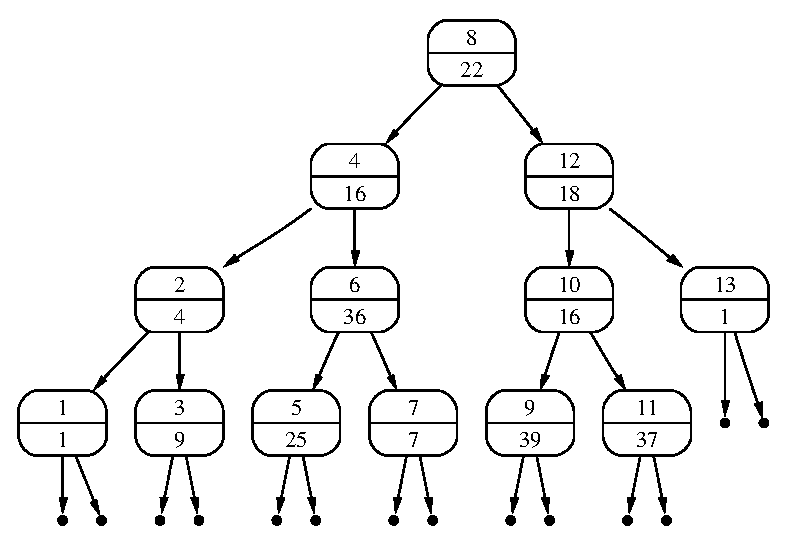
\epsfig{file=Abbildungen/graph1.eps}} 
  \caption{Ein geordneter bin\"arer Baum}
  \label{fig:graph1}
\end{figure}


Wir \"uberlegen uns nun, wie wir mit Hilfe geordneter bin\"arer B\"aume den ADT \textsl{Map}
implementieren k\"onnen.  Wir spezifizieren die einzelnen Methoden dieses Daten-Typs durch
(bedingte) Gleichungen.  Der Konstruktor $\textsl{Map}()$ liefert als Ergebnis den leeren Baum zur\"uck:
\[ \textsl{Map}() = \textsl{nil}. \]
F\"ur die Methode $\textsl{find}()$ erhalten wir die folgenden Gleichungen:
\begin{enumerate}
\item $\textsl{nil}\mathtt{.}\textsl{find}(k) = \Omega$,

      denn der leere Baum repr\"asentiert die leere Abbildung.
\item $\textsl{node}(k, v, l, r)\mathtt{.}\textsl{find}(k) = v$,

      denn der Knoten $\textsl{node}(k,v,l,r)$ speichert die Zuordnung $k \mapsto v$.
\item $k_1 < k_2 \rightarrow \textsl{node}(k_2, v, l, r)\mathtt{.}\textsl{find}( k_1) = l\mathtt{.}\textsl{find}(k_1)$,

      denn wenn $k_1$ kleiner als $k_2$ ist, dann kann aufgrund der Ordnungs-Bedingung
      eine Zuordnung f\"ur $k_1$ nur in dem linken Teilbaum $l$ gespeichert sein.
\item $k_1 > k_2 \rightarrow \textsl{node}(k_2, v, l, r)\mathtt{.}\textsl{find}( k_1 ) = r\mathtt{.}\textsl{find}(k_1)$,

      denn wenn $k_1$ gr\"o{\ss}er als $k_2$ ist, dann kann aufgrund der Ordnungs-Bedingung
      eine Zuordnung f\"ur $k_1$ nur in dem rechten Teilbaum $r$ gespeichert sein.
\end{enumerate}
Als n\"achstes definieren wir die Funktion \textsl{insert}.  Die Definition erfolgt
ebenfalls mit Hilfe rekursiver Gleichungen und ist ganz analog zur Definition der 
Funktion \textsl{find}.
\begin{enumerate}
\item $\textsl{nil}\mathtt{.}\textsl{insert}(k,v) = \textsl{node}(k,v, \textsl{nil}, \textsl{nil})$,
  
      denn wenn der Baum vorher leer ist, so kann die einzuf\"ugende Information direkt an
      der Wurzel abgespeichert werden.
\item $\textsl{node}(k, v_2, l, r)\mathtt{.}\textsl{insert}(k,v_1) = \textsl{node}(k, v_1, l, r)$,

      denn wenn wir den Schl\"ussel $k$ an der Wurzel finden, \"uberschreiben wir einfach den zugeordneten 
      Wert.
\item $k_1 < k_2 \rightarrow 
          \textsl{node}(k_2, v_2, l, r)\mathtt{.}\textsl{insert}(k_1, v_1) =
          \textsl{node}\bigl(k_2, v_2, l\mathtt{.}\textsl{insert}(k_1, v_1), r\bigr)$,

      denn wenn der Schl\"ussel $k_1$, unter dem wir Informationen einf\"ugen wollen, kleiner
      als der Schl\"ussel $k_2$ an der Wurzel ist, so m\"ussen wir die einzuf\"ugende
      Information im linken Teilbaum einf\"ugen.
\item $k_1 > k_2 \rightarrow 
         \textsl{node}(k_2, v_2, l, r)\mathtt{.}\textsl{insert}(k_1, v_1) = 
         \textsl{node}\bigl(k_2, v_2, l, r\mathtt{.}\textsl{insert}(k_1, v_1)\bigr)$,

      denn wenn der Schl\"ussel $k_1$, unter dem wir Informationen einf\"ugen wollen, gr\"o{\ss}er
      als der Schl\"ussel $k_2$ an der Wurzel ist, so m\"ussen wir die einzuf\"ugende
      Information im rechten Teilbaum einf\"ugen.
\end{enumerate}
Als letztes definieren wir die Methode \textsl{delete}. Diese Definition ist schwieriger als
die Implementierung der andern beiden Methoden.  Falls wir in einen Baum der Form
$t =\textsl{node}(k,v,l,r)$ den Eintrag mit dem Schl\"ussel $k$ l\"oschen wollen, so
kommt es auf die beiden Teilb\"aume $l$ und $r$ an.  Ist $l$ der leere Teilbaum,
so liefert $t\mathtt{.}\textsl{delete}(k)$ als Ergebnis den Teilbaum $r$ zur\"uck.
Ist $r$ der leere Teilbaum, so ist das Ergebnis $l$.  Problematisch ist die Situation,
wenn weder $l$ noch $r$ leer sind.  
Die L\"osung besteht dann darin, dass wir in dem rechten
Teilbaum $r$ den Knoten mit dem kleinsten Schl\"ussel suchen und diesen Knoten aus dem
Baum $r$ entfernen.  Den dadurch entstehenden Baum nennen wir $r'$.
 Anschlie{\ss}end \"uberschreiben wir in $t =\textsl{node}(k,v,l,r')$ die
Werte $k$ und $v$ mit dem eben gefundenen kleinsten Schl\"ussel $k_{min}$ und dem $k_{min}$
zugeordneten Wert $v_{min}$.  Der dadurch entstehende bin\"are Baum 
$t=\textsl{node}(k_{min},v_{min},l,r')$
 ist auch wieder
geordnet, denn einerseits ist der Schl\"ussel $k_{min}$  gr\"o{\ss}er als der Schl\"ussel $k$ und
damit sicher auch gr\"o{\ss}er als alle Schl\"ussel im linken Teilbaum $l$ und andererseits ist
$k_{min}$ kleiner als alle  Schl\"ussel im Teilbaum $r'$ den $k_{min}$ ist ja der
kleinste Schl\"ussel aus $r$.  

Zur Veranschaulichung betrachten wir ein Beispiel: Wenn wir in dem Baum aus Abbildung 
\ref{fig:graph1} den Knoten mit der Markierung $\pair(4,16)$ l\"oschen wollen,
so suchen wir zun\"achst in dem Teilbaum, dessen Wurzel mit $\pair(6,36)$ markiert ist, den
Knoten, der mit dem kleinsten Schl\"ussel markiert ist.  Dies ist der Knoten mit der
Markierung $\pair(5,25)$.  Wir l\"oschen diesen Knoten und \"uberschreiben die Markierung
$\pair(4,16)$ mit der Markierung $\pair(5,25)$.  Abbildung 
\ref{fig:graph2} auf Seite \pageref{fig:graph2} zeigt das Ergebnis.

\begin{figure}[!th]
  \centering
  \framebox{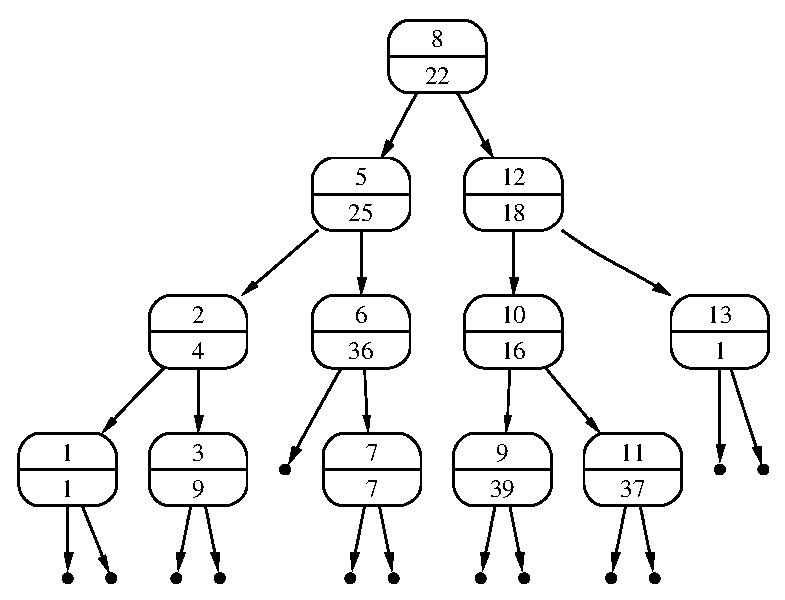
\epsfig{file=graph2.eps}} 
  \caption{Der geordnete bin\"arer Baum aus Abbildung 
          \ref{fig:graph1} nach dem Entfernen des Knotens mit der Markierung $\pair(4,16)$.}
  \label{fig:graph2}
\end{figure}

Wir geben nun bedingte Gleichungen an, die die Methode \textsl{delMin} spezifizieren.
\begin{enumerate}
\item $\textsl{node}(k, v, \textsl{nil}, r)\mathtt{.}\textsl{delMin}() = [r, k, v]$,

      denn wenn der linke Teilbaum leer ist, muss $k$ der kleinste Schl\"ussel in 
      dem Baum sein.  Wenn wir diesen  Schl\"ussel nebst dem zugeh\"origen Wert aus dem Baum
      entfernen, bleibt der rechte Teilbaum \"ubrig.

\item $l\not= \textsl{nil} \wedge l\mathtt{.}\textsl{delMin}() = [l',k_{min}, v_{min}] \;\rightarrow$ \\[0.1cm]
       \hspace*{1.3cm} 
       $\textsl{node}(k, v, l, r)\mathtt{.}\textsl{delMin}() = [\textsl{node}(k, v, l', r), k_{min}, v_{min}]$,

      denn wenn der linke Teilbaum $l$ in dem bin\"aren Baum $t = \textsl{node}(k, v, l, r)$
      nicht leer ist, so muss der kleinste Schl\"ussel von $t$ in $l$ liegen.
      Wir entfernen daher rekursiv den kleinsten Schl\"ussel aus $l$ und erhalten dabei den
      Baum $l'$.  In dem urspr\"unglich gegebenen Baum $t$ ersetzen wir $l$ durch $l'$ und erhalten
      $t = \textsl{node}(k, v, l', r)$.
\end{enumerate}
Damit k\"onnen wir nun die Methode $\mathtt{delete}()$ spezifizieren.
\begin{enumerate}
\item $\textsl{nil}\mathtt{.}\textsl{delete}(k) = \textsl{nil}$.
\item $\textsl{node}(k,v,\textsl{nil},r)\mathtt{.}\textsl{delete}(k) = r$.
\item $\textsl{node}(k,v,l,\textsl{nil})\mathtt{.}\textsl{delete}(k) = l$.
\item $l \not= \textsl{nil} \,\wedge\, r \not= \textsl{nil} \,\wedge\, r\mathtt{.}\textsl{delMin}() = [r',k_{min}, v_{min}]  \;\rightarrow$ \\[0.1cm]
      \hspace*{1.3cm}
      $\textsl{node}(k,v,l,r)\mathtt{.}\textsl{delete}(k) = \textsl{node}(k_{min},v_{min},l,r')$.
      
      Falls der zu entfernende Schl\"ussel mit dem Schl\"ussel an der Wurzel des Baums
      \"ubereinstimmt,  entfernen wir mit dem Aufruf $r\mathtt{.}\textsl{delMin}()$
      den kleinsten Schl\"ussel aus dem rechten Teilbaum  $r$ und produzieren dabei den Baum $r'$.
      Gleichzeitig berechnen wir dabei f\"ur den rechten Teilbaum den kleinsten Schl\"ussel $k_{min}$ und den
      diesem Schl\"ussel zugeordneten Wert $v_{min}$.  Diese Werte setzen wir nun an die
      Wurzel des neuen Baums.

\item $k_1 < k_2 \rightarrow \textsl{node}(k_2,v_2,l,r)\mathtt{.}\textsl{delete}(k_1) = 
       \textsl{node}\bigl(k_2,v_2,l\mathtt{.}\textsl{delete}(k_1),r\bigr)$,

      Falls der zu entfernende Schl\"ussel kleiner ist als der Schl\"ussel an der Wurzel,
      so kann sich der Schl\"ussel nur im linken Teilbaum befinden.  Daher wird der
      Schl\"ussel $k_1$ rekursiv in dem linken Teilbaum $l$ entfernt.
\item $k_1 > k_2 \rightarrow \textsl{node}(k_2,v_2,l,r)\mathtt{.}\textsl{delete}(k_1) = 
       \textsl{node}\bigl(k_2,v_2,l,r\mathtt{.}\textsl{delete}(k_1)\bigr)$,

      denn in diesem Fall kann sich der Eintrag mit dem Schl\"ussel $k_1$  nur im rechten Teilbaum befinden.
\end{enumerate}

\subsection{Implementierung geordneter bin\"arer B\"aume in \textsl{Java}}
\begin{figure}[!ht]
  \centering
\begin{Verbatim}[ frame         = lines, 
                  framesep      = 0.3cm, 
                  labelposition = bottomline,
                  numbers       = left,
                  numbersep     = -0.2cm,
                  xleftmargin   = 0.8cm,
                  xrightmargin  = 0.8cm
                ]
    public interface MyMap<Key extends Comparable<Key>, Value>
    {
        public Value find(Key key);
        public void  insert(Key key, Value value);
        public void  delete(Key key);
    }
\end{Verbatim}
\vspace*{-0.3cm}
  \caption{Das Interface  \textsl{MyMap}.}
  \label{fig:MyMap.java}
\end{figure}

Abbildung \ref{fig:MyMap.java} auf Seite \pageref{fig:MyMap.java} zeigt, 
wie sich der abstrakte Daten-Typ \textsl{Map} in \textsl{Java} durch ein
Interface beschreiben l\"asst.  Das Interface hat den Namen \textsl{MyMap}, denn da der ADT
\textsl{Map} von  fundamentaler Bedeutung ist, gibt es in \textsl{Java} bereits ein
Interface mit dem Namen \textsl{Map}.  Vergleichen wir die Signaturen der Methoden in dem
Interface \textsl{MyMap} mit den entsprechenden Signaturen in dem ADT \textsl{Map}, so
stellen wir fest, dass die Methoden \texttt{insert()} und \texttt{delete()} in dem
Interface den R\"uckgabewert \texttt{void} an Stelle von \textsl{MyMap} haben.
Anstatt also eine ge\"anderte Map zur\"uck zu geben \"andern diese Methoden die Map, mit der sie
aufgerufen werden.  Dies ist einerseits aus Effizienz-Gr\"unden wichtig und macht
andererseits die Verwendung dieser Methoden einfacher.


\begin{figure}[!ht]
  \centering
\begin{Verbatim}[ frame         = lines, 
                  framesep      = 0.3cm, 
                  labelposition = bottomline,
                  numbers       = left,
                  numbersep     = -0.2cm,
                  xleftmargin   = 0.8cm,
                  xrightmargin  = 0.8cm
                ]
    public class BinaryTree<Key extends Comparable<Key>, Value> 
        implements MyMap<Key, Value>
    {
        Node<Key, Value> mRoot;  
    
        public BinaryTree() {
            mRoot = new EmptyNode<Key, Value>();
        }
        public Value find(Key key) {
            return mRoot.find(key);
        }    
        public void insert(Key key, Value value) {
            mRoot = mRoot.insert(key, value);
        }
        public void delete(Key key) {
            mRoot = mRoot.delete(key);
        }
        // Transform the tree into a sorted list.
        public  LinkedList<Key> toList() {
            return mRoot.toList();
        }
    }
\end{Verbatim}
\vspace*{-0.3cm}
  \caption{Die Klasse \textsl{BinaryTree}.}
  \label{fig:BinTree.java}
\end{figure}



\begin{figure}[!ht]
  \centering
\begin{Verbatim}[ frame         = lines, 
                  framesep      = 0.3cm, 
                  labelposition = bottomline,
                  numbers       = left,
                  numbersep     = -0.2cm,
                  xleftmargin   = 0.8cm,
                  xrightmargin  = 0.8cm
                ]
    public abstract class Node<Key extends Comparable<Key>, Value>
    {
        public abstract Value find(Key key);
        public abstract Node<Key, Value> insert(Key key, Value value);
        public abstract Node<Key, Value> delete(Key key);
        public abstract boolean isEmpty();
        public abstract LinkedList<Key> toList();
    
        abstract Triple<Node<Key, Value>, Key, Value> delMin();
    }
\end{Verbatim}
\vspace*{-0.3cm}
  \caption{Die abstrakte Klasse \textsl{Node}.}
  \label{fig:Node.java}
\end{figure}

\begin{figure}[!ht]
  \centering
\begin{Verbatim}[ frame         = lines, 
                  framesep      = 0.3cm, 
                  labelposition = bottomline,
                  numbers       = left,
                  numbersep     = -0.2cm,
                  xleftmargin   = 0.8cm,
                  xrightmargin  = 0.8cm
                ]
    public class EmptyNode<Key extends Comparable<Key>, Value> 
        extends Node<Key, Value>
    {
        public EmptyNode() {}
        
        public Value find(Key key) {
            return null;
        }        
        public Node<Key, Value> insert(Key key, Value value) {
            return new BinaryNode<Key, Value>(key, value);
        }        
        public Node<Key, Value> delete(Key key) {
            return this;
        }
        public boolean isEmpty() {
            return true;
        }    
        public LinkedList<Key> toList() {
            return new LinkedList<Key>();
        }
        Triple<Node<Key, Value>, Key, Value> delMin() {
            throw new UnsupportedOperationException();
        }
    }
\end{Verbatim}
\vspace*{-0.3cm}
  \caption{Die Klasse \textsl{EmptyNode}.}
  \label{fig:EmptyNode.java}
\end{figure}

Abbildung \ref{fig:BinTree.java} auf Seite \pageref{fig:BinTree.java} zeigt die 
Implementierung der Klasse \textsl{BinTree} in \textsl{Java}.  Die Klasse enth\"alt ein
Objekt vom Typ \textsl{Node} mit dem Namen \texttt{mRoot}.  Dieser Knoten repr\"asentiert
die Wurzel des bin\"aren Baums.  Die Methoden der Klasse \textsl{BinTree} werden dadurch
implementiert, dass die analogen Methoden der abstrakten Klasse \textsl{Node} aufgerufen
werden.  
Abbildung \ref{fig:Node.java} auf Seite \pageref{fig:Node.java} zeigt die Definition
der Klasse \textsl{Node}.  Bei der Betrachtung der Signaturen der Methoden stellen wir
fest, dass die Methoden \textsl{insert()} und \textsl{delete()} nun einen R\"uckgabewert
haben.   Dies ist n\"otig, weil in \textsl{Java} ein Objekt seinen Typ nicht \"andern kann.  
Von der Klasse \textsl{Node} werden zwei konkrete Klassen abgeleitet:  Die Klasse
\textsl{EmptyNode} repr\"asentiert einen leeren bin\"aren Baum, entspricht also dem
\textsl{nil} und die Klasse \textsl{BinaryNode} dient dazu, einen Knoten der Form
$\textsl{node}(k,v,l,r)$ darzustellen.  Nun ist es so, dass beim Einf\"ugen  aus
einem leeren Baum ein nicht-leerer Baum werden kann und umgekehrt kann beim L\"oschen 
aus einem nicht-leeren Baum ein leerer Baum werden.  Da aber die Methode \textsl{insert()}
ein Objekt vom Typ \textsl{EmptyNode} nicht in ein Objekt \textsl{BinaryNode} umwandeln
kann, muss die Methode \textsl{insert()} stattdessen den bin\"aren Baum, der durch das
Einf\"ugen eines Schl\"ussels entsteht, als Ergebnis zur\"uck geben.  Analoges gilt f\"ur die
Methode \textsl{delete()}.

\begin{figure}[!ht]
  \centering
\begin{Verbatim}[ frame         = lines, 
                  framesep      = 0.3cm, 
                  labelposition = bottomline,
                  numbers       = left,
                  numbersep     = -0.2cm,
                  xleftmargin   = 0.0cm,
                  xrightmargin  = 0.0cm
                ]
    public class BinaryNode<Key extends Comparable<Key>, Value> 
        extends Node<Key, Value>
    {
        private Key              mKey;     /**< The key stored at the root. */
        private Value            mValue;   /**< The value attached to this key. */
        private Node<Key, Value> mLeft;    /**< The left subtree. */
        private Node<Key, Value> mRight;   /**< The right subtree. */
    
        public BinaryNode(Key key, Value value) {
            mKey   = key;
            mValue = value;
            mLeft  = new EmptyNode<Key, Value>();
            mRight = new EmptyNode<Key, Value>();
        }        
        public Value find(Key key) {
            int cmp = key.compareTo(mKey);
            if (cmp < 0) {                // key < mKey
                return mLeft.find(key);
            } else if (cmp > 0) {         // key > mKey
                return mRight.find(key);
            } else {                      // key == mKey
                return mValue;
            }            
        }
        public Node<Key, Value> insert(Key key, Value value) {
            int cmp = key.compareTo(mKey);
            if (cmp < 0) {                        // key < mKey
                mLeft = mLeft.insert(key, value);
            } else if (cmp > 0) {                 // key > mKey
                mRight = mRight.insert(key, value);
            } else {                              // key == mKey
                mValue = value;
            }            
            return this;
        }
\end{Verbatim}
\vspace*{-0.3cm}
  \caption{Die Klasse \textsl{BinaryNode}, Teil \texttt{I}.}
  \label{fig:BinaryNode-I.java}
\end{figure}

\begin{figure}[!ht]
  \centering
\begin{Verbatim}[ frame         = lines, 
                  framesep      = 0.3cm, 
                  firstnumber   = last,
                  labelposition = bottomline,
                  numbers       = left,
                  numbersep     = -0.2cm,
                  xleftmargin   = 0.0cm,
                  xrightmargin  = 0.0cm
                ]
        public Node<Key, Value> delete(Key key) {
            int cmp = key.compareTo(mKey);
            if (cmp == 0) {
                if (mLeft.isEmpty()) {
                    return mRight;
                } 
                if (mRight.isEmpty()) {
                    return mLeft;
                }
                Triple triple = mRight.delMin();
                mRight = triple.getFirst();
                mKey   = triple.getSecond();
                mValue = triple.getThird();
            }
            if (cmp < 0) {
                mLeft = mLeft.delete(key);
            }
            if (cmp > 0) {
                mRight = mRight.delete(key);
            }
            return this;
        }    
        public boolean isEmpty() {
            return false;
        }
        Triple delMin() {
            if (mLeft.isEmpty()) {
                return new Triple<Node<Key, Value>, Key, Value>(mRight, mKey, mValue);
            } else {
                Triple<Node<Key, Value>, Key, Value> t = mLeft.delMin();
                      mLeft = t.getFirst();
                Key   key   = t.getSecond();
                Value value = t.getThird();
                return new Triple<Node<Key, Value>, Key, Value>(this, key, value);
            }
        }        
    }
\end{Verbatim}
\vspace*{-0.3cm}
  \caption{Die Klasse \textsl{BinaryNode}, Teil \texttt{II}.}
  \label{fig:BinaryNode-II.java}
\end{figure}
\vspace*{0.1cm}

Gegen\"uber den Methoden aus der Klasse \textsl{BinaryTree} hat die Klasse \textsl{Node} die
zus\"atzliche Methode \textsl{isEmpty()} die \"uberpr\"uft, ob der Knoten den leeren Baum
repr\"asentiert. Au{\ss}erdem gibt es noch die Methode \textsl{delMin()}, die den Knoten mit dem
kleinsten Schl\"ussel aus einem Baum l\"oscht.  Diese Methode ist nicht als \texttt{public}
deklariert, da sie nur zur Implementierung der Methode \textsl{delete()} benutzt wird.


Abbildung \ref{fig:EmptyNode.java} zeigt die Definition der Klasse \textsl{EmptyNode}.
Bemerkenswert ist hier die Implementierung der Methode \textsl{delMin()}: Da der leere
Baum keine Schl\"ussel enth\"alt, macht die Methode \textsl{delMin()} keinen Sinn.  Daher
produziert der Aufruf dieser Methode eine Ausnahme.


Algorithmisch interessant ist die Implementierung der Klasse \textsl{BinaryNode}, die in den
Abbildungen \ref{fig:BinaryNode-I.java} und \ref{fig:BinaryNode-II.java} auf den Seiten 
\pageref{fig:BinaryNode-I.java} und \pageref{fig:BinaryNode-II.java} gezeigt wird.
Die Klasse enth\"alt vier Member-Variablen:
\begin{enumerate}
\item \texttt{mKey} ist der Schl\"ussel, der an diesem Knoten abgespeichert wird.
\item \texttt{mValue} ist der dem Schl\"ussel \textrm{mKey} zugeordnete Wert.
\item \texttt{mLeft} ist der linke Teilbaum.
\item \texttt{mRight} ist der rechte Teilbaum.
\end{enumerate}
Ein Objekt $o$ der Klasse \textsl{BinaryNode} entspricht also dem Term \\[0.1cm]
\hspace*{1.3cm} 
$\textsl{node}(o.\texttt{mKey}, o.\texttt{mValue}, o.\texttt{mLeft}, o.\texttt{mRight})$. 
\\[0.1cm]
Die Implementierung der Methoden \textsl{find()}, \textsl{insert()} und \textsl{delete()} setzt die bedingten
Gleichungen, mit denen wir diese Methoden spezifiziert haben, eins-zu-eins um.

\begin{figure}[!ht]
  \centering
\begin{Verbatim}[ frame         = lines, 
                  framesep      = 0.3cm, 
                  firstnumber   = last,
                  labelposition = bottomline,
                  numbers       = left,
                  numbersep     = -0.2cm,
                  xleftmargin   = 0.8cm,
                  xrightmargin  = 0.8cm
                ]
    public class Triple<First, Second, Third>
    {
        First  mFirst;
        Second mSecond;
        Third  mThird;
        
        Triple(First first, Second second, Third value) {
            mFirst  = first;
            mSecond = second;
            mThird  = value;
        }
    
        First  getFirst()  { return mFirst;  }
        Second getSecond() { return mSecond; }
        Third  getThird()  { return mThird;  }
    }
\end{Verbatim}
\vspace*{-0.3cm}
  \caption{Die Klasse \textsl{Triple}.}
  \label{fig:Triple.java}
\end{figure}

\noindent
Abbildung \ref{fig:Triple.java} auf Seite \pageref{fig:Triple.java} zeigt schlie{\ss}lich die
Implementierung der Klasse \textsl{Triple}.  Diese Klasse dient dazu ein Tripel
darzustellen und hat folglich drei Member-Variablen \texttt{mFirst}, \texttt{mSecond},
\texttt{mThird}, die jeweils die erste, zweite und dritte Komponente des Tripels abspeichern.
\pagebreak



\subsection{Analyse der Komplexit\"at}
Wir untersuchen zun\"achst die Komplexit\"at der Funktion \textsl{find} im schlechtesten Fall.
Dieser Fall tritt dann ein, wenn der bin\"are Baum zu einer Liste entartet.  Abbildung
\ref{fig:degenerated} zeigt den geordneten bin\"aren Baum der dann entsteht, wenn die Paare
aus Schl\"ussel und Werten aus der Abbildung
\ref{fig:graph1} in aufsteigender Reihenfolge eingegeben werden.  Wird hier nach dem
gr\"o{\ss}ten Schl\"ussel gesucht, so muss der komplette Baum durchlaufen werden.  Enth\"alt der Baum
$n$ Schl\"ussel, so sind also insgesamt $n$ Vergleiche erforderlich.  In diesem Fall ist ein
geordneter bin\"arer Baum also nicht besser als eine Liste.

\begin{figure}[!th]
  \centering
  \framebox{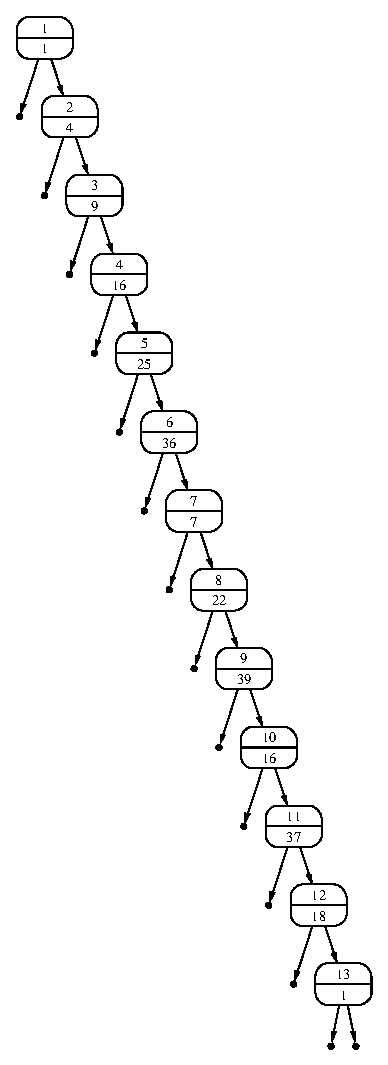
\epsfig{file=degenerated-bin-tree}} 
  \caption{Ein entarteter  geordneter bin\"arer Baum.}
  \label{fig:degenerated}
\end{figure}

Erfreulicherweise tritt der schlechteste Fall im statistischen Durchschnitt selten auf.
Im Durchschnitt ist ein zuf\"allig erzeugter bin\"arer Baum recht gut balanciert, so dass 
beispielsweise f\"ur einen Aufruf von \texttt{find()} f\"ur einen Baum mit $n$ Schl\"usseln
durchschnittlich  $\Oh\bigl(\ln(n)\bigr)$
Vergleiche erforderlich sind. Wir werden diese Behauptung nun beweisen.

%Dazu definieren wir auf bin\"aren B\"aumen zun\"achst eine Funktion 
%\[ \textsl{height}: \Bin \rightarrow \N, \]
%die die H\"ohe eines bin\"aren Baums angibt.  Die Definition erfolgt induktiv.
%\begin{enumerate}
%\item $\textsl{nil}.\textsl{height}() = 0$.

%      Der leere Baum hat die H\"ohe $0$.
%\item $\textsl{node}(k,v,l,r).\textsl{height}() = 
%       1 + \max\bigl(l.\textsl{height}(),\, r.\textsl{height}()\bigr)$.

%      Die H\"ohe des Baums $\textsl{node}(k,v,l,r)$ ist um eins gr\"o{\ss}er als die H\"ohe des
%      gr\"o{\ss}ten Teilbaums.
%\end{enumerate}
%Analog definieren wir f\"ur einen bin\"aren Baum $b$ die Anzahl $b.\textsl{count}()$ der Schl\"ussel, die
%der Baum enth\"alt.   Die Definition von $b.\textsl{count}()$ erfolgt durch Induktion nach $b$.
%\begin{enumerate}
%\item $\textsl{nil}.\textsl{count}() = 0$.

%      Der leere Baum enth\"alt keine Schl\"ussel.
%\item $\textsl{node}(k,v,l,r).\textsl{count}() = 
%       1 + l.\textsl{count}() + r.\textsl{height}()\bigr)$.

%      Der Baum $\textsl{node}(k,v,l,r)$ enth\"alt zus\"atzlich zu dem Schl\"ussel $k$ die
%      Schl\"ussel aus den Teilb\"aumen $l$ und $r$.
%\end{enumerate}
%Der folgende Satz zeigt, wieviel Schl\"ussel ein Baum der H\"ohe $h$ h\"ochstens enthalten
%kann.

%\begin{Satz}
%  Ein bin\"arer Baum $b$ der H\"ohe $h$ enth\"alt h\"ochstens $2^h - 1$ Schl\"ussel.
%\end{Satz}
%\noindent
%\textbf{Beweis}:  Wir bezeichnen die maximale Anzahl Schl\"ussel eines Baums der H\"ohe $h$
%mit $c_h$.  Wir beweisen  durch Induktion nach $h$, dass gilt:
%\[ c_h = 2^h - 1. \]
%\begin{enumerate}
%\item[I.A.] $h = 0$: Der einzige Baum der H\"ohe $0$ ist $\textsl{nil}$.
%            Dieser enth\"alt $0$ Schl\"ussel.  Also gilt
%            \\[0.2cm]
%            \hspace*{1.3cm}
%            $c_0 = 0 = 2^0 - 1$.
%\item[I.S.] $h \mapsto h + 1$: Ein Baum der H\"ohe $h+1$, der die maximale Anzahl
%            Schl\"ussel enth\"alt, hat die Form $\textsl{node}(k,v,l,r)$, wobei dann $l$ und
%            $r$  B\"aume der H\"ohe $h$ sind, die die maximale Anzahl Schl\"ussel enthalten.
%            Folglich gilt:
%            \begin{eqnarray*}
%               c_{h+1} &               =  & 1 + c_h + c_h \\
%                       & \stackrel{IV}{=} & 1 + (2^h - 1) + (2^h - 1) \\
%                       &               =  & 2 \cdot 2^h - 1 \\
%                       &               =  & 2^{h+1} - 1. \hspace*{9cm} \Box
%            \end{eqnarray*}
%\end{enumerate}

%Die H\"ohe eines Baumes gibt ein Ma{\ss} f\"ur die Komplexit\"at der Methoden \textsl{find},
%\textsl{insert} und \textsl{delete}, denn bei einem Baum der H\"ohe $h$ sind f\"ur jede dieser
%Operationen h\"ochstens $h$ Vergleiche von Schl\"usseln erforderlich.

Wir bezeichnen die \underline{durchschnittliche} Anzahl von Vergleichen, die beim Aufruf
$b.\textsl{find}(k)$ f\"ur einen geordneten bin\"aren Baum $b$ durchgef\"uhrt werden m\"ussen, falls $b$
insgesamt $n$ Schl\"ussel enth\"alt, mit $d_n$.  Wir wollen annehmen, dass der Schl\"ussel $k$ auch
wirklich in $b$ zu finden ist.  Unser Ziel ist es, f\"ur $d_n$ eine Rekurrenz-Gleichung aufzustellen.
Zun\"achst
ist klar, dass \\[0.2cm]
\hspace*{1.3cm} $d_1 = 1$ \\[0.2cm]
ist, denn wenn der Baum $b$ nur einen Schl\"ussel enth\"alt, wird genau einen Vergleich durchgef\"uhrt.
Wir betrachten nun einen bin\"aren Baum $b$, der $n+1$ Schl\"ussel enth\"alt.  Dann hat $b$
die Form \\[0.2cm]
\hspace*{1.3cm} $b = \textsl{node}(k',v,l,r)$. \\[0.2cm]
Ordnen wir die $n+1$ Schl\"ussel der Gr\"o{\ss}e nach in der Form 
\\[0.2cm]
\hspace*{1.3cm}
$k_0 < k_1 < \cdots < k_i < k_{i+1} < k_{i+2} < \cdots < k_{n-1} < k_n$,
\\[0.2cm]
so gibt es $n+1$ verschiedene Positionen, an denen
der Schl\"ussel $k'$ auftreten kann.  Wenn $k' = k_i$ ist, so enth\"alt der
linke Teilbaum $i$ Schl\"ussel und der rechte Teilbaum enth\"alt $n-i$ Schl\"ussel:
\\[0.2cm]
\hspace*{1.3cm}
$\underbrace{k_0 < k_1 < \cdots < k_{i-1}}_{\mbox{Schl\"ussel in $l$}} < 
 \underbrace{k_{i}}_{\stackrel{\displaystyle \shortparallel}{\displaystyle k'}} < 
 \underbrace{k_{i+1} < \cdots < k_{n-1} < k_n}_{\mbox{Schl\"ussel in $r$}}$,
\\[0.2cm]
Da $b$ insgesamt $n+1$ Schl\"ussel enth\"alt, gibt es $n+1$ M\"oglichkeiten, wie die
verbleibenden $n$ Schl\"ussel auf die beiden Teilb\"aume $l$ und $r$ verteilt sein k\"onnen, denn
$l$ kann $i$ Schl\"ussel enthalten, wobei \\[0.2cm]
\hspace*{1.3cm} $i \in \{0,1, \cdots, n\}$ \\[0.2cm]
gilt.  Entsprechend enth\"alt $r$ dann $n-i$ Schl\"ussel.  
Bezeichnen wir die durchschnittliche Anzahl von Vergleichen in einem Baum mit $n+1$
Schl\"usseln, dessen linker Teilbaum $i$ Elemente hat, mit
\\[0.2cm]
\hspace*{1.3cm}
$\textsl{anzVgl}(i,\, n\!+\!1)$,
\\
so gilt
\\[-0.1cm]
\hspace*{1.3cm}
$d_{n+1} = \sum\limits_{i=0}^n \bruch{1}{n+1} \cdot \textsl{anzVgl}(i,\, n\!+\!1)$,
\\[0.2cm]
denn wir haben ja angenommen, dass alle Werte von $i$ die gleiche Wahrscheinlichkeit,
n\"amlich $\frac{1}{n+1}$, haben.
\vspace*{0.1cm}

Berechnen wir nun den Wert von $\textsl{anzVgl}(i,n\!+\!1)$:
Falls $l$ aus $i$ Schl\"usseln besteht und die restlichen $n-i$ Schl\"ussel in $r$ liegen,
so gibt es f\"ur den Schl\"ussel $k$, nach dem wir in dem Aufruf $b.\textsl{find}(k)$ suchen, 
$3$ M\"oglichkeiten:
\begin{enumerate}
\item $k$ kann mit dem Schl\"ussel $k'$ an der Wurzel des Baums \"ubereinstimmen.
      In diesem Fall f\"uhren wir nur einen Vergleich durch.  Da es insgesamt
      $n+1$ Schl\"ussel in dem Baum gibt und nur in einem dieser F\"alle
      der Schl\"ussel, den wir suchen, an der Wurzel steht, hat dieser Fall die
      Wahrscheinlichkeit
      \\[0.2cm]
      \hspace*{1.3cm} $\bruch{1}{\,n+1\,}$.

\item $k$ kann mit einem der $i$ Schl\"ussel im linken Teilbaum $l$ \"ubereinstimmen.
      Da  der linke Teilbaum $i$ Schl\"ussel enth\"alt und  es insgesamt
      $n+1$ Schl\"ussel gibt, hat die Wahrscheinlichkeit, dass $k$ in dem linken Teilbaum $l$
      auftritt, den Wert \\[0.2cm]
      \hspace*{1.3cm} $\displaystyle\bruch{i}{n+1}$. \\[0.2cm]
       In diesem Fall werden \\[0.2cm]
      \hspace*{1.3cm} $\displaystyle d_i + 1$ \\[0.2cm]
      Vergleiche durchgef\"uhrt, denn au{\ss}er den $d_i$ Vergleichen mit den Schl\"usseln aus dem
      linken Teilbaum muss der Schl\"ussel, der gesucht wird, ja noch mit dem Schl\"ussel an
      der Wurzel verglichen werden.
\item $k$ kann mit einem der $n-i$ Schl\"ussel im rechten Teilbaum $r$ \"ubereinstimmen.

      Da  der rechte Teilbaum $n-i$ Schl\"ussel enth\"alt und  es insgesamt
      $n+1$ Schl\"ussel gibt, hat die Wahrscheinlichkeit, dass $k$ in dem rechten Teilbaum $r$
      auftritt, den Wert \\[0.2cm]
      \hspace*{1.3cm} $\displaystyle \bruch{n-i}{n+1}$. \\[0.2cm]
      Analog zum zweiten Fall werden diesmal \\[0.2cm]
      \hspace*{1.3cm} $\displaystyle d_{n-i} + 1$ \\[0.2cm]
      Vergleiche durchgef\"uhrt. 
\end{enumerate}
Um nun  $\textsl{anzVgl}(i, n\!+\!1)$ berechnen zu k\"onnen, m\"ussen wir in jedem der drei
F\"alle die Wahrscheinlichkeit mit der Anzahl der Vergleiche multiplizieren und
die Werte, die sich f\"ur die drei F\"alle ergeben, aufsummieren.  Wir erhalten
\begin{eqnarray*}
  \textsl{anzVgl}(i, n\!+\!1) 
& = & \bruch{1}{\,n+1\,} \cdot 1 + \bruch{i}{n+1} \cdot (d_i + 1) + \bruch{n-i}{n+1} \cdot (d_{n-i} + 1) 
      \\[0.2cm]
& = & \bruch{1}{\,n+1\,} \cdot \bigl(1 + i \cdot (d_i + 1) + (n-i) \cdot (d_{n-i} + 1)\bigr)      \\[0.2cm]
& = & \bruch{1}{\,n+1\,} \cdot \bigl(1 + i + (n-i) + i \cdot d_i + (n-i) \cdot d_{n-i} \bigr)    \\[0.2cm]
& = & \bruch{1}{\,n+1\,} \cdot \bigl(n + 1 + i \cdot d_i + (n-i) \cdot d_{n-i} \bigr)            \\[0.2cm]
& = & 1 + \bruch{1}{\,n+1\,} \cdot \bigl(i \cdot d_i + (n-i) \cdot d_{n-i} \bigr) 
\end{eqnarray*}


Damit k\"onnen wir nun die Rekurrenz-Gleichung f\"ur $d_{n+1}$ aufstellen: 
\[
\begin{array}{lcl}
d_{n+1} 
& = &  
\sum\limits_{i=0}^n \bruch{1}{\,n+1\,} \cdot \textsl{anzVgl}(i,\,n\!+\!1)  \\[0.5cm]
& = &  
\bruch{1}{n+1} \cdot \sum\limits_{i=0}^n  
           \left(1 + \bruch{1}{n+1} \cdot \bigl(i \cdot d_i + (n-i) \cdot d_{n-i} \bigr) \right)
\\[0.5cm]
& = &  
\bruch{1}{n+1} \cdot \Biggl(\underbrace{\sum\limits_{i=0}^n 1}_{\stackrel{\displaystyle \shortparallel}{n+1}} \;+\;
           \bruch{1}{n+1} \cdot \sum\limits_{i=0}^n \bigl(i \cdot d_i + (n-i) \cdot d_{n-i} \bigr) \Biggr)
\\[1.3cm]
& = &  
1 + \bruch{1}{(n+1)^2} \cdot \left(\sum\limits_{i=0}^n \left(i\cdot d_i + (n-i)\cdot d_{n-i}\right) \right) 
\\[0.5cm]
& = &  
1 + \bruch{2}{(n+1)^2} \cdot \sum\limits_{i=0}^n i\cdot d_i 
\end{array}
\]
Bei der letzten Umformung haben wir die Gleichung (\ref{eq:qssum}) \\[0.2cm]
\hspace*{1.3cm} $\sum\limits_{i=0}^n f(n-i) = \sum\limits_{i=0}^n f(i)$ \\[0.2cm]
benutzt, die wir bei der Analyse der Komplexit\"at von Quick-Sort gezeigt hatten.
Wir l\"osen jetzt die Rekurrenz-Gleichung 
\begin{equation}
  \label{eq:bin1}
d_{n+1} = \displaystyle 1 + \bruch{2}{(n+1)^2} \cdot \sum\limits_{i=0}^n i\cdot d_i  
\end{equation}
mit der Anfangs-Bedingungen $d_1 = 1$.  
Zur L\"osung von Gleichung (\ref{eq:bin1}) f\"uhren wir die Substitution $n \mapsto n+1$ durch und erhalten 
\begin{equation}
  \label{eq:bin2}
d_{n+2} = \displaystyle 1 + \bruch{2}{(n+2)^2} \cdot \sum\limits_{i=0}^{n+1} i\cdot d_i  
\end{equation}
Wir multiplizieren nun Gleichung (\ref{eq:bin1}) mit $(n+1)^2$ und Gleichung (\ref{eq:bin2}) 
mit $(n+2)^2$ und finden die Gleichungen 
\begin{eqnarray}
  \label{eq:bin3}
(n+1)^2 \cdot d_{n+1} & = & (n+1)^2 + 2 \cdot \sum\limits_{i=0}^n i\cdot d_i, \\
  \label{eq:bin4}
(n+2)^2 \cdot d_{n+2} & = & (n+2)^2 + 2 \cdot \sum\limits_{i=0}^{n+1} i\cdot d_i
\end{eqnarray}
Subtrahieren wir Gleichung (\ref{eq:bin3}) von Gleichung (\ref{eq:bin4}),
so erhalten wir \\[0.2cm]
\hspace*{1.3cm} 
$(n+2)^2 \cdot d_{n+2} - (n+1)^2 \cdot d_{n+1} = (n+2)^2 - (n+1)^2 + 2 \cdot (n+1) \cdot d_{n+1}$.
\\[0.2cm]
Zur Vereinfachung substituieren wir hier $n \mapsto n - 1$ und erhalten \\[0.2cm]
\hspace*{1.3cm} 
$(n+1)^2 \cdot d_{n+1} - n^2 \cdot d_{n} = (n+1)^2 - n^2 + 2 \cdot n \cdot d_{n}$.
\\[0.2cm]
Dies vereinfachen wir zu \\[0.2cm]
\hspace*{1.3cm} $(n+1)^2 \cdot d_{n+1}  =  n \cdot (n + 2) \cdot d_{n} + 2 \cdot n + 1$. \\[0.2cm]
Bei dieser Gleichung teilen wir auf beiden Seiten durch $(n+2)\cdot (n+1)$ und bekommen \\[0.2cm]
\hspace*{1.3cm}  
$\displaystyle \bruch{n+1}{n+2} \cdot d_{n+1}  =  \bruch{n}{n + 1} \cdot d_{n} + \bruch{2 \cdot n + 1}{(n+2)\cdot (n+1)}$. \\[0.2cm]
Nun definieren wir \\[0.2cm]
\hspace*{1.3cm} $\displaystyle c_n = \bruch{n}{n+1} \cdot d_n$. \\[0.2cm]
Dann gilt $c_1 = \bruch{1}{2} \cdot d_1 = \bruch{1}{2}$ und wir  haben die Rekurrenz-Gleichung \\[0.2cm]
\hspace*{1.3cm} 
$\displaystyle c_{n+1}  =  c_{n} + \frac{2 \cdot n + 1}{(n+2)\cdot (n+1)}$. \\[0.2cm]
Durch Partialbruch-Zerlegung finden wir \\[0.2cm]
\hspace*{1.3cm} 
$\displaystyle \frac{2 \cdot n + 1}{(n+2)\cdot (n+1)} = \frac{3}{n+2} - \frac{1}{n+1}$. \\[0.2cm]
Also haben wir \\[0.2cm]
\hspace*{1.3cm} $\displaystyle c_{n+1} = c_n +  \frac{3}{n+2} - \frac{1}{n+1}$. \\[0.2cm]
Wegen $c_1 = \bruch{1}{2}$ ist die Gleichung auch f\"ur $n=0$ richtig, wenn wir $c_0 = 0$ setzen, denn es gilt
\\[0.2cm]
\hspace*{1.3cm}
$\bruch{1}{2} = 0 + \bruch{3}{0+2} - \bruch{1}{0+1}$.
\\[0.2cm]
Die Rekurrenz-Gleichung f\"ur $c_n$ k\"onnen wir mit dem Teleskop-Verfahren l\"osen:
\begin{eqnarray*}  
  c_{n+1} & = & c_0 + \sum\limits_{i=0}^{n} \frac{3}{i+2} - \sum\limits_{i=0}^{n} \frac{1}{i+1} 
\\[0.2cm]
          & = & \sum\limits_{i=2}^{n+2} \frac{3}{i} - \sum\limits_{i=1}^{n+1} \frac{1}{i}.
\end{eqnarray*}
Wir substituieren $n \mapsto n-1$ und vereinfachen dies zu 
\\[0.2cm]
\hspace*{1.3cm}
$c_{n} =  \displaystyle\sum\limits_{i=2}^{n+1} \frac{3}{i} - \sum\limits_{i=1}^{n} \frac{1}{i}$
\\[0.2cm]
Die harmonische Zahl $H_n$ ist als
\\[0.2cm]
\hspace*{1.3cm}
$H_n = \sum\limits_{i=1}^{n} \bruch{1}{i}$   
\\[0.2cm]
definiert.  Wir k\"onnen $c_n$ auf $H_n$ zur\"uckf\"uhren: 
\begin{eqnarray*}
   c_n & = & 3 \cdot H_n - \bruch{3}{1} + \bruch{3}{n+1} - H_n \\
       & = & 2 \cdot H_n - 3 \cdot \frac{n}{n+1} 
\end{eqnarray*}
Wegen $H_n = \displaystyle\sum\limits_{i=1}^{n} \frac{1}{i} = \ln(n) + \Oh(1)$ gilt dann \\[0.2cm]
\hspace*{1.3cm} 
$\displaystyle c_n = 2 \cdot \ln(n) + \Oh(1)$.
\\[0.2cm]
Ber\"ucksichtigen wir  $d_n = \bruch{n+1}{n}\cdot c_n$, so finden wir f\"ur gro{\ss}e $n$ ebenfalls \\[0.2cm]
\hspace*{1.3cm} $\displaystyle d_n = 2 \cdot \ln(n) + \Oh\bigl(1\bigr)$.
\\[0.2cm]
Das ist unser zentrales Ergebnis: Im Durchschnitt erfordert das Suchen in einem zuf\"allig
erzeugten geordneten bin\"aren Baum f\"ur gro{\ss}e Werte von $n$ etwa 
\\[0.2cm]
\hspace*{1.3cm}
$2 \cdot \ln(n) = 2 \cdot \ln(2) \cdot \log_2(n) \approx 1.386 \cdot \log_2(n)$ 
\\[0.2cm]
Vergleiche.  Damit werden etwa 39 \% 
mehr Vergleiche ausgef\"uhrt als bei einem optimal balancierten bin\"aren Baum.
\"Ahnliche Ergebnisse k\"onnen wir f\"ur das Einf\"ugen oder L\"oschen erhalten.

%%% Local Variables: 
%%% mode: latex
%%% TeX-master: "algorithmen"
%%% End: 

\section{AVL Trees}
If a binary tree is approximately \blue{balanced}, i.e.~if the left and right subtree of a binary tree $b$  have
roughly the same height, then the complexity of $b.\texttt{find}(k)$ will always be of the order
$\Oh\bigl(\ln(n)\bigr)$.  There are a number of different variations of
balanced binary trees.  Of these variations, the species of balanced binary trees that is the easiest to understand is
called an \href{https://en.wikipedia.org/wiki/AVL_tree}{AVL tree} \cite{adelson:62}.  AVL trees are 
named after their inventors \href{https://en.wikipedia.org/wiki/Georgy_Adelson-Velsky}{Georgy M.~Adelson-Velsky} 
(1922 -- 2014) and \href{https://en.wikipedia.org/wiki/Evgenii_Landis}{Evgenii~M.~Landis} (1921 -- 1997).  
In order to define these trees we need to define the \blue{height} of a binary tree formally:
\begin{enumerate}
\item $\texttt{Nil}.\texttt{height}() = 0$.
\item $\texttt{Node}(k,v,l,r).\texttt{height}() = 
       \max\bigl( l.\texttt{height}(), r.\texttt{height}() \bigr) + 1$. \eox
\end{enumerate}

\begin{Definition}[AVL-Tree] \hspace*{\fill} \\
{\em 
  The set $\AVL$ of \blue{AVL trees} is defined inductively:
  \begin{enumerate}
  \item $\texttt{Nil} \in \AVL$.
  \item $\texttt{Node}(k,v,l,r) \in \AVL$ \quad iff 
        \begin{enumerate}
        \item $\texttt{Node}(k,v,l,r) \in \Bin_<$,
        \item $l, r \in \AVL$, \quad and
        \item $|l.\texttt{height}() - r.\texttt{height}()| \leq 1$.

              This condition is called the \blue{balancing condition}.
        \end{enumerate}
        According to this definition, an AVL tree is an ordered binary tree such that for every node
        $\texttt{Node}(k,v,l,r)$ in this tree the height of the left subtree $l$ and the right
        subtree  $r$ differ at most by one.  \qed
  \end{enumerate}
}  
\end{Definition}

In order to implement AVL trees we can start from our implementation of ordered binary trees.
In addition to those methods that we have already seen in the class $\texttt{Map}$ we will need the method
\\[0.2cm]
\hspace*{1.3cm} $\texttt{restore}: \Bin_< \rightarrow \AVL$. 
\\[0.2cm]
This method is used to restore the balancing condition at a given node if it has been violated by
either inserting or deleting an element.
The method call $b.\texttt{restore}()$ assumes that  $b$ is an ordered binary tree that satisfies
the balancing condition everywhere except possibly at its root. 
At the root, the height of the left subtree might differ from the height of the right subtree by at
most 2.  Hence, when the method $b.\texttt{restore}()$ is invoked we have either of the following
two cases:
\begin{enumerate}
\item $b = \texttt{Nil}$ \quad or
\item $b = \texttt{Node}(k,v,l,r) \wedge l \in \AVL \wedge r \in \AVL \wedge
       |l.\texttt{height}() - r.\texttt{height}()| \leq 2$.
\end{enumerate}
The method $\texttt{restore}$ is specified via conditional equations.
\begin{enumerate}
\item $\texttt{Nil}.\texttt{restore}() = \texttt{Nil}$,

      because the empty tree already is an  AVL tree.
\item $|l.\texttt{height}() - r.\texttt{height}()| \leq 1 \rightarrow 
       \texttt{Node}(k,v,l,r).\texttt{restore}() = \texttt{Node}(k,v,l,r)$.

      If the balancing condition is satisfied, then nothing needs to be done. 
\item $\begin{array}[t]{cl}
              & l_1.\texttt{height}() = r_1.\texttt{height}() + 2    \\ 
       \wedge & l_1 = \texttt{Node}(k_2,v_2,l_2,r_2)                 \\
       \wedge & l_2.\texttt{height}() \geq r_2.\texttt{height}()     \\[0.2cm]
       \rightarrow & \texttt{Node}(k_1,v_1,l_1,r_1).\texttt{restore}() = 
                     \texttt{Node}\bigl(k_2,v_2,l_2,\texttt{Node}(k_1,v_1,r_2,r_1)\bigr)
       \end{array}
      $

      The motivation for this equation can be found in Figure \ref{fig:casell}
      on page \pageref{fig:casell}.  The left part of this figure shows the state
      of the tree before it has been rebalanced.  Therefore, this part shows the tree
      \\[0.2cm]
      \hspace*{1.3cm}
      $\texttt{Node}(k_1,v_1, \texttt{Node}(k_2,v_2,l_2,r_2), r_1)$. 
      \\[0.2cm]
      The right part of Figure \ref{fig:casell} shows the effect of rebalancing.  
      This rebalancing results in the tree
      \\[0.2cm]
      \hspace*{1.3cm}
      $\texttt{Node}\bigl(k_2,v_2,l_2,\texttt{Node}(k_1,v_1,r_2,r_1)\bigr)$.
      \\[0.2cm]
      In Figure \ref{fig:casell} the label below the horizontal line of each node shows the height
      of the tree corresponding to this node.  For subtrees, the height is given below the name of
      the subtree.  For example,  $h$ is the height of the subtree 
      $l_2$, while $h-1$ is the height of the subtree $r_1$. The height of the subtree $r_2$
      is $h'$ and we know that $h' \leq h$.  As $\texttt{Node}(k_2,v_2,l_2,r_2)$ is an AVL tree and we know that
      $l_2.\texttt{height}() \geq r_2.\texttt{height}()$, we
      either have $h' = h$ or $h' = h-1$.

      The state shown in Figure \ref{fig:casell} can arise if either an element has been inserted
      in the left subtree $l_1$ or if an element has been deleted from the right subtree  $r_1$.

      \begin{figure}[!ht]
        \centering
        \framebox{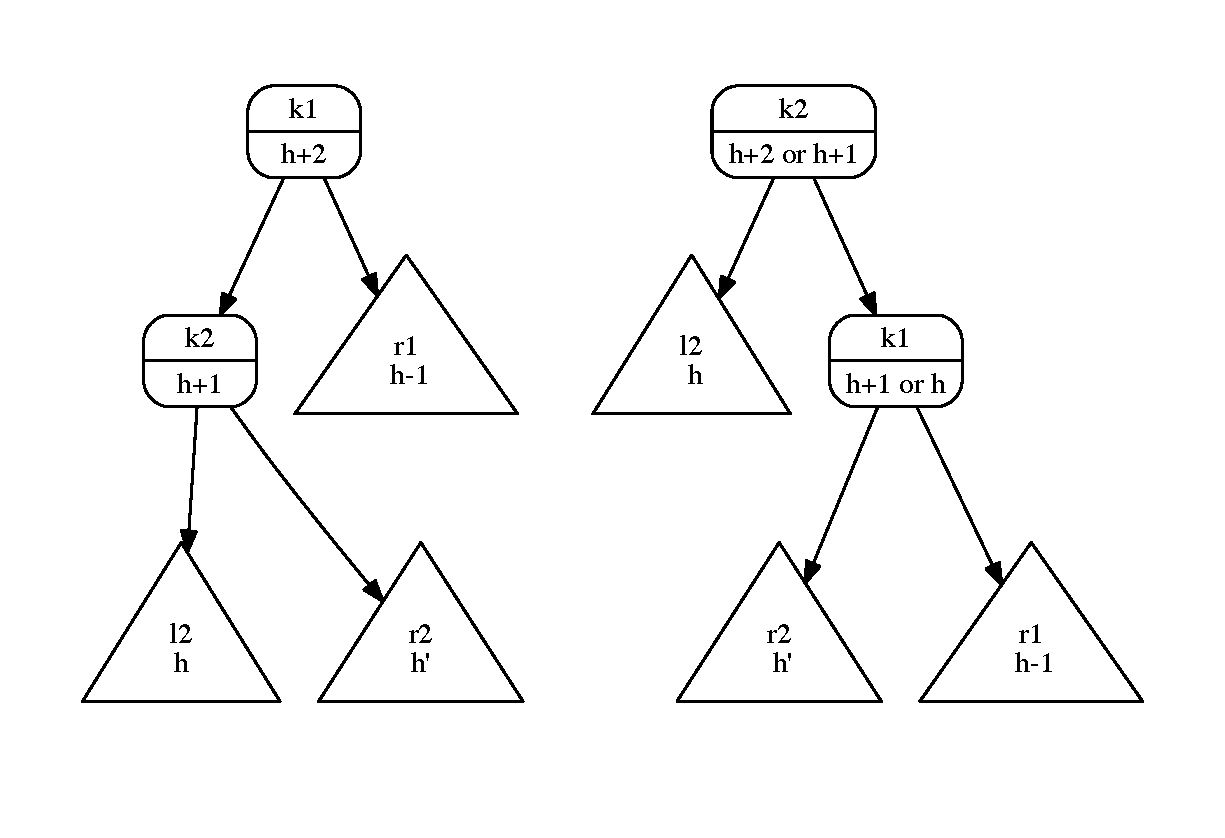
\epsfig{file=Abbildungen/casell.pdf,scale=0.7}} 
        \caption{An unbalanced tree and the corresponding rebalanced tree.}
        \label{fig:casell}
      \end{figure}
      We have to make sure that the tree shown in the right part of Figure
      \ref{fig:casell} is indeed an  AVL tree. With respect to the balancing condition this is
      easily verified.  The fact that the node containing the key $k_1$ has either the height
      $h$ or $h+1$ is a consequence of the fact that the height of $r_1$ is  $h-1$ while the height of $r_2$ is
      $h'$ and we know that $h' \in \{h, h-1\}$.

      In order to verify that the tree is ordered we can use the following inequation: 
      \\[0.2cm]
      \hspace*{1.3cm}
      $l_2 < k_2 < r_2 < k_1 < r_1$. 
      \hspace*{\fill} $(\star)$
      \\[0.2cm]
      Here we have used the following notation: If  $k$ is a key and  $b$ is a binary tree, then we write \\[0.2cm]
      \hspace*{1.3cm} $k < b$ \\[0.2cm]
      in order to express that  $k$ is smaller than all keys that occur in the tree  $b$.
      Similarly,  $b < k$ denotes the fact that all keys occurring in $b$ are less than the key
      $k$.  The inequation  $(\star)$ describes both the ordering of keys in the left part of Figure
      \ref{fig:casell} and in the right part of this figure.  Hence, the tree shown in the right
      part of Figure \ref{fig:casell} is ordered provided the tree in the left part is ordered to begin with.
\item $\begin{array}[t]{cl}
               & l_1.\texttt{height}() = r_1.\texttt{height}() + 2    \\ 
        \wedge & l_1 = \texttt{Node}(k_2,v_2,l_2,r_2)               \\
        \wedge & l_2.\texttt{height}() < r_2.\texttt{height}()     \\
        \wedge & r_2 = \texttt{Node}(k_3,v_3,l_3,r_3)               \\
        \rightarrow & \texttt{Node}(k_1,v_1,l_1,r_1).\texttt{restore}() = 
                      \texttt{Node}\bigl(k_3,v_3,\texttt{Node}(k_2,v_2,l_2,l_3),\texttt{Node}(k_1,v_1,r_3,r_1) \bigr)
        \end{array}
       $

       The left hand side of this equation is shown in Figure  \ref{fig:caselr} on page
       \pageref{fig:caselr}.  This tree can be written as
       \\[0.2cm]
       \hspace*{1.3cm} 
       $\texttt{Node}\bigl(k_1,v_1,\texttt{Node}(k_2,v_2,l_2,\texttt{Node}\bigl(k_3,v_3,l_3,r_3)\bigr),r_1\bigr)$. 
       \\[0.2cm]
       The subtrees $l_3$ and $r_3$ have either the height  $h$ or $h-1$.  Furthermore, at least one
       of these subtrees must have the height  $h$ for otherwise the subtree
       $\texttt{Node}(k_3,v_3,l_3,r_3)$ would not have the height $h+1$.
       
\begin{figure}[!ht]
  \centering
  \framebox{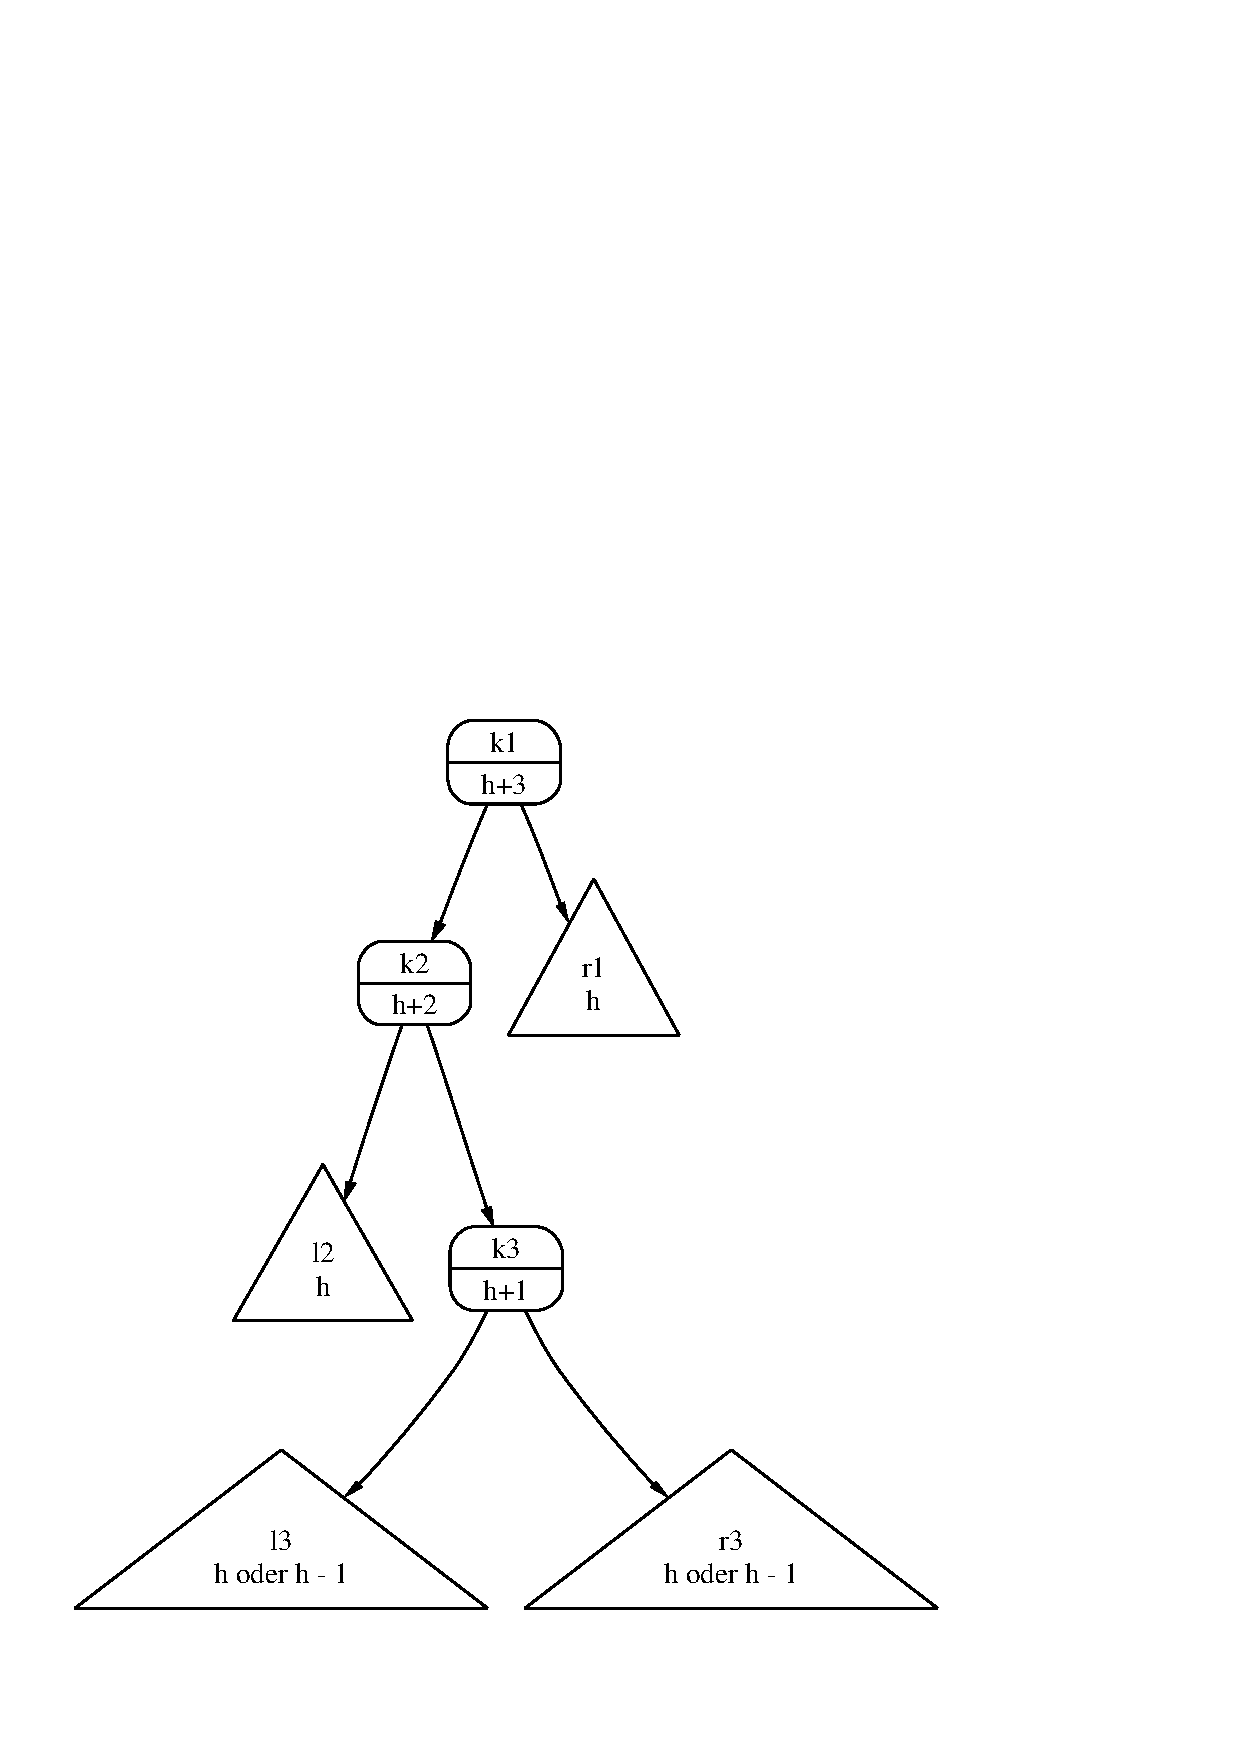
\epsfig{file=Abbildungen/caselr,scale=0.7}} 
  \caption{An unbalanced tree, second case.}
  \label{fig:caselr}
\end{figure}

     Figure \ref{fig:caselr-nach} on page \pageref{fig:caselr-nach} shows how the tree looks after
     rebalancing.  The tree shown in this figure has the form
     \\[0.2cm]
     \hspace*{1.3cm} 
     $\texttt{Node}\bigl(k_3,v_3,\texttt{Node}(k_2,v_2,l_2,l_3),\texttt{Node}(k_1,v_1,r_3,r_1) \bigr)$.


\begin{figure}[!ht]
  \centering
  \framebox{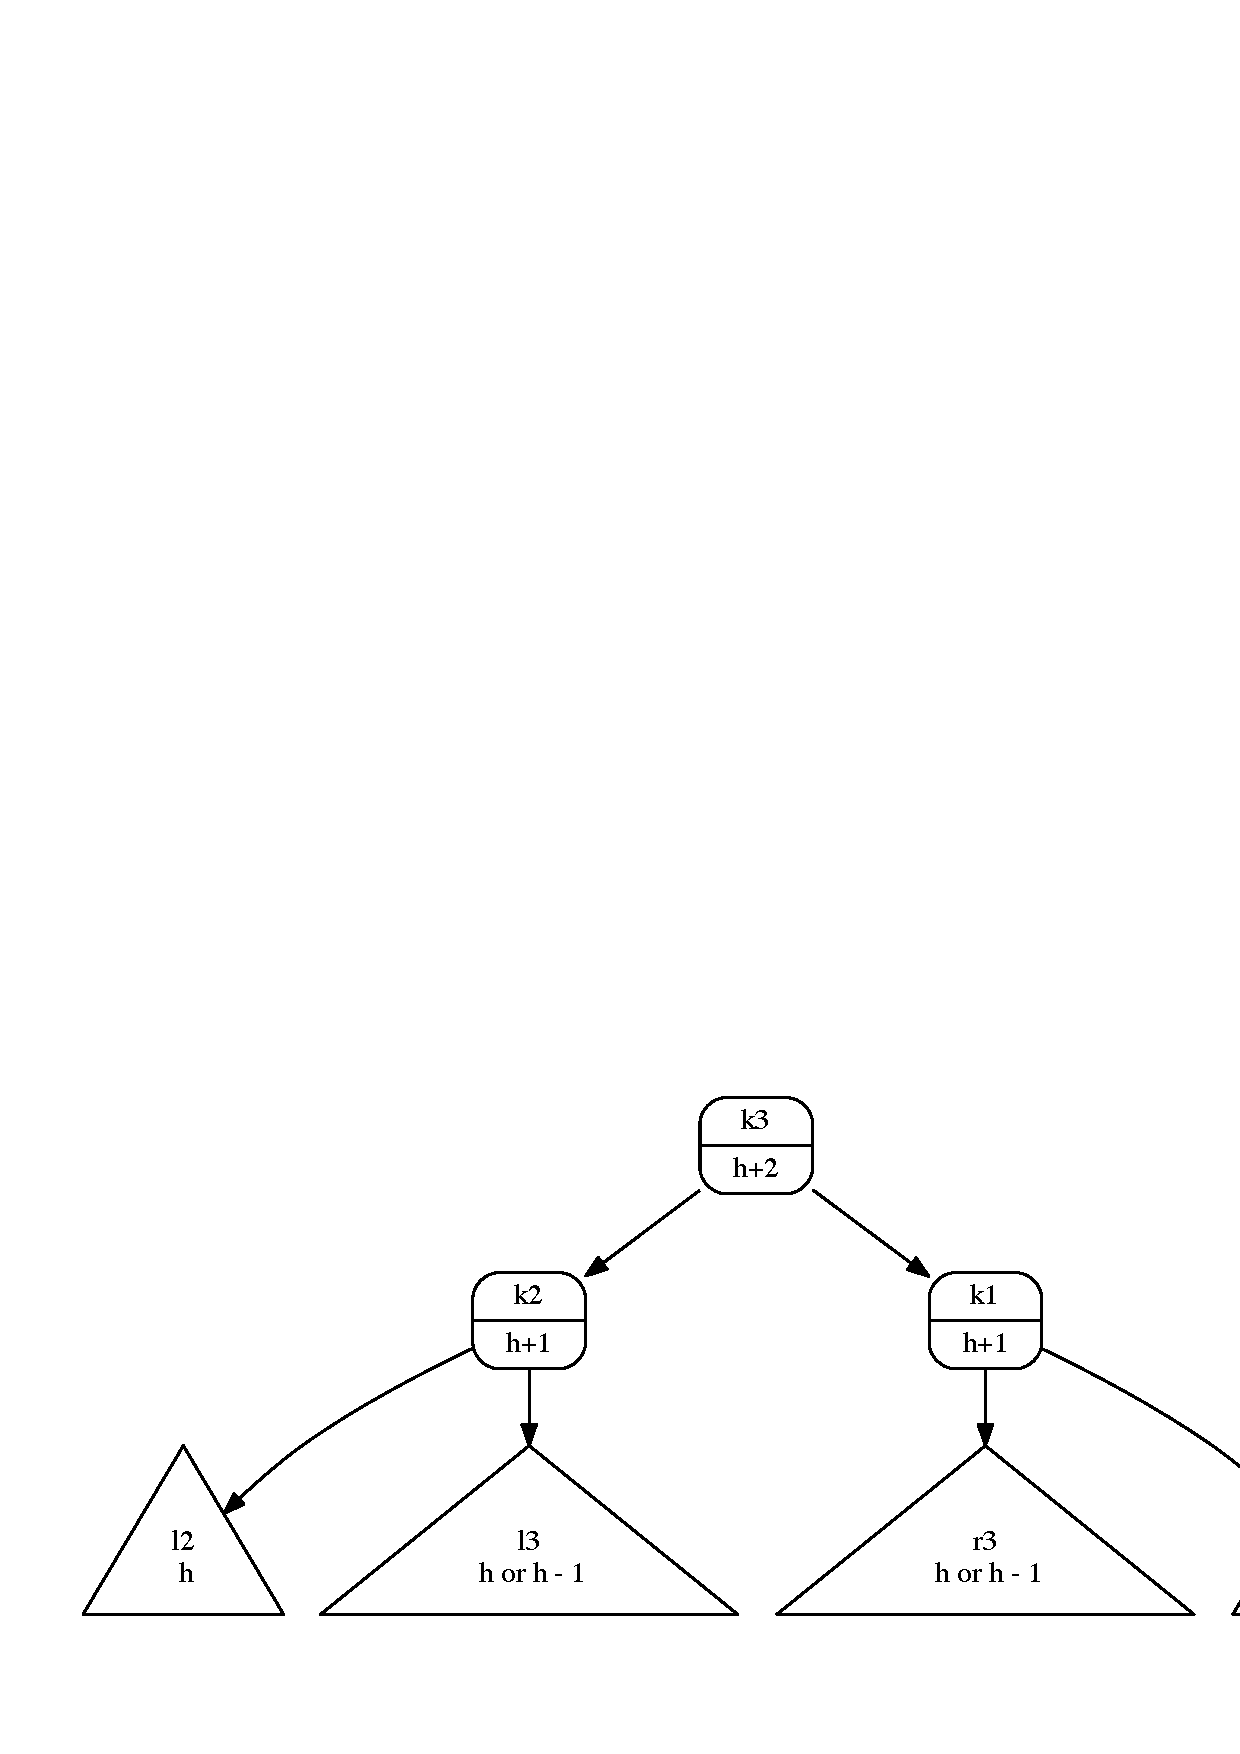
\epsfig{file=Abbildungen/caselr-nach,scale=0.7}} 
  \caption{The rebalanced tree in the second case.}
  \label{fig:caselr-nach}
\end{figure}

      The inequation describing the ordering of the keys both in the left subtree and in the right
      subtree is given as
      \\[0.2cm]
      \hspace*{1.3cm} $l_2 < k_2 < l_3 < k_3 < r_3 < k_1 < r_1$.

      There are two more cases where the height of the right subtree is bigger by more than 
      the height of the left subtree plus one.  These two cases are completely analogous to the two
      cases discussed previously.  Therefore we just state the corresponding equations without
      further discussion.
\item $\begin{array}[t]{cl}
              & r_1.\texttt{height}() = l_1.\texttt{height}() + 2    \\ 
       \wedge & r_1 = \texttt{Node}(k_2,v_2,l_2,r_2)               \\
       \wedge & r_2.\texttt{height}() \geq l_2.\texttt{height}()     \\[0.2cm]
       \rightarrow & \texttt{Node}(k_1,v_1,l_1,r_1).\texttt{restore}() = 
                     \texttt{Node}\bigl(k_2,v_2,\texttt{Node}(k_1,v_1,l_1,l_2),r_2\bigr)
       \end{array}
      $
\item $\begin{array}[t]{cl}
               & r_1.\texttt{height}() = l_1.\texttt{height}() + 2    \\ 
        \wedge & r_1 = \texttt{Node}(k_2,v_2,l_2,r_2)               \\
        \wedge & r_2.\texttt{height}() < l_2.\texttt{height}()     \\
        \wedge & l_2 = \texttt{Node}(k_3,v_3,l_3,r_3)               \\
        \rightarrow & \texttt{Node}(k_1,v_1,l_1,r_1).\texttt{restore}() = 
                      \texttt{Node}\bigl(k_3,v_3,\texttt{Node}(k_1,v_1,l_1,l_3),\texttt{Node}(k_2,v_2,r_3,r_2) \bigr)
        \end{array}
       $

\end{enumerate}
Now we are ready to specify the method  $\texttt{insert}()$ via recursive equations.
If we compare these equations to the equations we had given for unbalanced ordered binary trees we
notice that we only have to call the method $\texttt{restore}$ if the balancing condition might have
been violated.
\begin{enumerate}
\item $\texttt{Nil}.\texttt{insert}(k,v) = \texttt{Node}(k,v, \texttt{Nil}, \texttt{Nil})$.  
\item $\texttt{Node}(k, v_2, l, r).\texttt{insert}(k,v_1) = \texttt{Node}(k, v_1, l, r)$.
\item $k_1 < k_2 \rightarrow 
          \texttt{Node}(k_2, v_2, l, r).\texttt{insert}(k_1, v_1) =
          \texttt{Node}\bigl(k_2, v_2, l.\texttt{insert}(k_1,v_1), r\bigr).\texttt{restore}()$.
\item $k_1 > k_2 \rightarrow 
         \texttt{Node}(k_2, v_2, l, r).\texttt{insert}\bigl(k_1, v_1\bigr) = 
         \texttt{Node}\bigl(k_2, v_2, l, r.\texttt{insert}(k_1,v_1)\bigr).\texttt{restore}()$.
\end{enumerate}
The equations for  $\texttt{delMin}()$ change as follows:
\begin{enumerate}
\item $\texttt{Node}(k, v, \texttt{Nil}, r).\texttt{delMin}() = \langle r, k, v \rangle$.
\item $l\not= \texttt{Nil} \wedge \langle l',k_{min}, v_{min}\rangle := l.\texttt{delMin}() 
       \;\rightarrow$ \\[0.2cm]
       \hspace*{1.3cm} 
       $\texttt{Node}(k, v, l, r).\texttt{delMin}() = 
        \langle \texttt{Node}(k, v, l', r).\texttt{restore}(), k_{min}, v_{min} \rangle$.
\end{enumerate}
Finally, the equations for $\texttt{delete}$ are as follows:
\begin{enumerate}
\item $\texttt{Nil}.\texttt{delete}(k) = \texttt{Nil}$.
\item $\texttt{Node}(k,v,\texttt{Nil},r).\texttt{delete}(k) = r$.
\item $\texttt{Node}(k,v,l,\texttt{Nil}).\texttt{delete}(k) = l$.
\item $l \not= \texttt{Nil} \,\wedge\, r \not= \texttt{Nil} \,\wedge\, 
       \langle r',k_{min}, v_{min} \rangle := r.\texttt{delMin}()  \;\rightarrow$ \\[0.2cm]
      \hspace*{1.3cm}
      $\texttt{Node}(k,v,l,r).\texttt{delete}(k) = \texttt{Node}(k_{min},v_{min},l,r').\texttt{restore}()$.
\item $k_1 < k_2 \rightarrow \texttt{Node}(k_2,v_2,l,r).\texttt{delete}(k_1) = 
       \texttt{Node}\bigl(k_2,v_2,l.\texttt{delete}(k_1),r\bigr).\texttt{restore}()$.
\item $k_1 > k_2 \rightarrow \texttt{Node}(k_2,v_2,l,r).\texttt{delete}(k_1) = 
         \texttt{Node}\bigl(k_2,v_2,l,r.\texttt{delete}(k_1)\bigr).\texttt{restore}()$.
\end{enumerate}


\subsection{Implementing AVL-Trees in \textsl{Python}}
If we want to implement AVL-trees in \textsl{Python} then we have to decide how to compute the height
of the trees.  The idea is to store the height of every subtree in the corresponding node since it
would be inefficient if we would recompute this height every time we need it.  Therefore, we add a
member variable \texttt{mHeight} to our class map.
Figure \ref{fig:avl-tree.ipython:init} shows the constructor of the class \texttt{AVLTree}.  The variable
\texttt{mHeight} is defined in line 7.  It is initialised as $0$ since the constructor \texttt{\_\_init\_\_}
constructs an empty node.  

\begin{figure}[!ht]
  \centering
\begin{minted}[ frame         = lines, 
                framesep      = 0.3cm, 
                bgcolor       = sepia,
                numbers       = left,
                numbersep     = -0.2cm,
                xleftmargin   = 0.8cm,
                xrightmargin  = 0.8cm
              ]{python3}
    class AVLTree:
        def __init__(self):
            self.mKey    = None
            self.mValue  = None
            self.mLeft   = None
            self.mRight  = None
            self.mHeight = 0 
\end{minted}
\vspace*{-0.3cm}
  \caption{Outline of the class \texttt{map}.}
  \label{fig:avl-tree.ipython:init}
\end{figure}


Figure \ref{fig:avl-tree.ipython:find} shows the implementation of the function $\texttt{find}$.
Actually, the implementation is the same as the implementation in Figure
\ref{fig:binary-tree.py-1}.  The reason is that every AVL tree is also an ordered binary tree and
since searching for a key does not change the underlying tree there is no need to restore anything.

\begin{figure}[!ht]
\centering
\begin{minted}[ frame         = lines, 
                  framesep      = 0.3cm, 
                  firstnumber   = 1,
                  bgcolor = sepia,
                  numbers       = left,
                  numbersep     = -0.2cm,
                  xleftmargin   = 0.8cm,
                  xrightmargin  = 0.8cm,
                ]{python3}
    def find(self, key):
        if self.isEmpty():
            return
        elif self.mKey == key:
            return self.mValue
        elif key < self.mKey:
            return self.mLeft.find(key)
        else:
            return self.mRight.find(key)
\end{minted}
\vspace*{-0.3cm}
\caption{Implementation of the method $\texttt{find}$.}
\label{fig:avl-tree.ipython:find}
\end{figure}


Figure \ref{fig:avl-tree.ipython:insert} shows the implementation of the method $\texttt{insert}$.
If we compare this implementation with the implementation for ordered binary trees, we find three
differences.
\begin{enumerate}
\item When inserting into an empty tree, we now have to update the member variable \texttt{mHeight}
      to $1$.  This is done in line 7.
\item After inserting a key-value pair into the left subtree \texttt{mLeft}, it might be necessary to 
      rebalance the tree.  This is done in line 12.
\item Similarly, if we insert a key-value pair into the right subtree \texttt{mRight}, we have to rebalance 
      the tree.  This is done in line 15.
\end{enumerate}

\begin{figure}[!ht]
\centering
\begin{minted}[ frame         = lines, 
                  framesep      = 0.3cm, 
                  firstnumber   = 1,
                  bgcolor = sepia,
                  numbers       = left,
                  numbersep     = -0.2cm,
                  xleftmargin   = 0.8cm,
                  xrightmargin  = 0.8cm,
                ]{python3}
    def insert(self, key, value):
        if self.isEmpty():
            self.mKey    = key
            self.mValue  = value
            self.mLeft   = AVLTree()
            self.mRight  = AVLTree()
            self.mHeight = 1
        elif self.mKey == key:
            self.mValue = value
        elif key < self.mKey:
            self.mLeft.insert(key, value)
            self._restore()
        else:
            self.mRight.insert(key, value)
            self._restore()
\end{minted}
\vspace*{-0.3cm}
\caption{Implementation of the method $\texttt{insert}$.}
\label{fig:avl-tree.ipython:insert}
\end{figure}

Figure \ref{fig:avl-tree.ipython:delMin} shows the implementation of the method \texttt{delMin}.
The only change compared to the previous implementation for ordered binary trees is in line 7, where
we have to take care of the fact that the balancing condition might be violated after deleting the
smallest element in the left subtree.

\begin{figure}[!ht]
\centering
\begin{minted}[ frame         = lines, 
                framesep      = 0.3cm, 
                firstnumber   = 1,
                bgcolor = sepia,
                numbers       = left,
                numbersep     = -0.2cm,
                xleftmargin   = 0.8cm,
                xrightmargin  = 0.8cm,
              ]{python3}
    def _delMin(self):
        if self.mLeft.isEmpty():
            return self.mRight, self.mKey, self.mValue
        else:
            ls, km, vm = self.mLeft._delMin()
            self.mLeft = ls
            self._restore()
            return self, km, vm
\end{minted}
\vspace*{-0.3cm}
\caption{Implementation of \texttt{delMin}.}
\label{fig:avl-tree.ipython:delMin}
\end{figure}


Figure \ref{fig:avl-tree.ipython:delete} shows the implementation of the method $\texttt{delete}$ and the
implementation of the auxiliary method \texttt{update}.  Compared with Figure
\ref{fig:binary-tree.py-2} there are only three differences:
\begin{enumerate}
\item If we delete the key at the root of the tree, we replace this key with the smallest key in the
      right subtree. Since this key is deleted in the right subtree, the height of the right
      subtree might shrink and hence the balancing condition at the root might be violated.
      Therefore, we have to restore the balancing condition.  This is done in line 12.
\item If we delete a key in the left subtree, the height of the left subtree might shrink.
      Hence we have to rebalance the tree at the root in line 15.
\item Similarly, if we delete a key in the right subtree, we have to restore the balancing
      condition.  This is done in line 18.
\end{enumerate}
Since the method \texttt{update} replaces the current tree with either its left or right subtree and this
subtree is assumed to satisfy the balancing condition, there is no need for a call to \texttt{restore} in this
method. 

\begin{figure}[!ht]
\centering
\begin{minted}[ frame         = lines, 
                framesep      = 0.3cm, 
                firstnumber   = 1,
                bgcolor = sepia,
                numbers       = left,
                numbersep     = -0.2cm,
                xleftmargin   = 0.8cm,
                xrightmargin  = 0.8cm,
              ]{python3}
    def delete(self, key):
        if self.isEmpty():
            return
        if key == self.mKey:
            if self.mLeft.isEmpty():
                self._update(self.mRight)
            elif self.mRight.isEmpty():
                self._update(self.mLeft)
            else:
                self.mRight, self.mKey, self.mValue = \
                     self.mRight._delMin()
                self._restore()
        elif key < self.mKey:
            self.mLeft.delete(key)
            self._restore()
        else:
            self.mRight.delete(key)
            self._restore() 

    def _update(self, t):
        self.mKey    = t.mKey
        self.mValue  = t.mValue
        self.mLeft   = t.mLeft
        self.mRight  = t.mRight
        self.mHeight = t.mHeight            
\end{minted}
\vspace*{-0.3cm}
\caption{The methods $\texttt{delete}$ and \texttt{update}.}
\label{fig:avl-tree.ipython:delete}
\end{figure}
\begin{figure}[!ht]
\centering
\begin{minted}[ frame         = lines, 
                framesep      = 0.3cm, 
                firstnumber   = 1,
                bgcolor = sepia,
                numbers       = left,
                numbersep     = -0.2cm,
                xleftmargin   = 0.0cm,
                xrightmargin  = 0.0cm,
              ]{python3}
    def _restore(self):
        if abs(self.mLeft.mHeight - self.mRight.mHeight) <= 1:
            self._restoreHeight()
            return
        if self.mLeft.mHeight > self.mRight.mHeight:
            k1,v1,l1,r1 = self.mKey,self.mValue,self.mLeft,self.mRight
            k2,v2,l2,r2 = l1.mKey, l1.mValue, l1.mLeft, l1.mRight
            if l2.mHeight >= r2.mHeight:
                self._setValues(k2, v2, l2, createNode(k1,v1,r2,r1))
            else: 
                k3,v3,l3,r3 = r2.mKey,r2.mValue,r2.mLeft,r2.mRight
                self._setValues(k3, v3, createNode(k2, v2, l2, l3),
                                        createNode(k1, v1, r3, r1))
        elif self.mRight.mHeight > self.mLeft.mHeight:
            k1,v1,l1,r1 = self.mKey,self.mValue,self.mLeft,self.mRight
            k2,v2,l2,r2 = r1.mKey, r1.mValue, r1.mLeft, r1.mRight
            if r2.mHeight >= l2.mHeight:
                self._setValues(k2, v2, createNode(k1,v1,l1,l2), r2)
            else:
                k3,v3,l3,r3 = l2.mKey,l2.mValue,l2.mLeft,l2.mRight
                self._setValues(k3, v3, createNode(k1, v1, l1, l3),
                                        createNode(k2, v2, r3, r2))
        self._restoreHeight()
    
    def _setValues(self, k, v, l, r):
        self.mKey   = k
        self.mValue = v
        self.mLeft  = l
        self.mRight = r
    
    def _restoreHeight(self):
        self.mHeight = max(self.mLeft.mHeight, self.mRight.mHeight)+1
\end{minted}
\vspace*{-0.3cm}
\caption{The implementation of \texttt{restore} and \texttt{restoreHeight}.}
\label{fig:avl-tree.ipython:restore}
\end{figure}


Figure \ref{fig:avl-tree.ipython:restore} shows the implementation of the function \texttt{restore}.
It is this method that makes most of the difference between ordered binary trees and AVL trees.  Let
us discuss this method line by line.
\begin{enumerate}
\item In line 2 we check whether the balancing condition is satisfied.  If we are lucky,  this test 
      is successful and hence we do not need to restore the structure of the tree.  However, we
      still need to maintain the height of the tree since it is possible that variable
      \texttt{mHeight} no longer contains the correct height.  For example, assume that the left subtree
      initially has a height that is bigger by one than the height of the right subtree.  Assume
      further that we have deleted a node in the left subtree so that its height shrinks.  Then the
      balancing condition is still satisfied, as now the left subtree and the right subtree have the
      same height.  However, the height of the complete tree has also shrunk by one and therefore, 
      the variable \texttt{mHeight} needs to be decremented.  This is done via the auxiliary method
      \texttt{restoreHeight}.  This method is defined in line 31 and it recomputes \texttt{mHeight}
      according to the definition of the height of a binary tree.
\item If the check in line 2 fails, then we know that the balancing condition is violated.
      However, we do not yet know which of the two subtrees is bigger.  

      If the test in line 5 succeeds, then the left subtree must have a height that is bigger by
      two than the height of the right subtree.  In order to be able to use the same variable names 
      as the variable names given in the equations discussed in the previous subsection, we define
      the variables \texttt{k1}, \texttt{v1}, \texttt{l1}, \texttt{r1}, \texttt{k2}, \texttt{v2}, \texttt{l2},
      and \texttt{r2} in line 6 and 7 so that these variable names correspond exactly to the variable names
      used in the Figures \ref{fig:casell} and \ref{fig:caselr}.
\item Next, the test in line 8 checks whether we have the case that is depicted in Figure
      \ref{fig:casell}.  In this case, Figure \ref{fig:casell} tells us that the key \texttt{k2}
      has to move to the root.  The left subtree is now \texttt{l2}, while the right subtree is a
      new node that has the key \texttt{k1} at its root.  This new node is created by the call
      of the function \texttt{createNode} in line 9.  The function \texttt{createNode} is shown in
      Figure \ref{fig:avl-tree.ipython:createNode} on page \pageref{fig:avl-tree.ipython:createNode}.
\item If the test in line 8 fails, the right subtree is bigger than the left subtree and we are in 
      the case that is depicted in Figure \ref{fig:caselr}.  We have to create the tree that is
      shown in Figure \ref{fig:caselr-nach}.  To this end we first define the variables 
      \texttt{k3}, \texttt{v3}, \texttt{l3}, and \texttt{r3} in a way that these variables
      correspond to the variables shown in Figure \ref{fig:caselr}.  Next, we create the tree
      that is shown in Figure \ref{fig:caselr-nach}.
\item Line 14 deals with the case that the right subtree is bigger than the left subtree. 
      As this case is analogous to the case covered in line 5 to line 13, we won't discuss this case
      any further.
\item Finally, we recompute the variable \texttt{mHeight} since it is possible that the old value is
      no longer correct.
\end{enumerate}


\begin{figure}[!ht]
\centering
\begin{minted}[ frame         = lines, 
                framesep      = 0.3cm, 
                firstnumber   = 1,
                bgcolor = sepia,
                numbers       = left,
                numbersep     = -0.2cm,
                xleftmargin   = 0.8cm,
                xrightmargin  = 0.8cm,
              ]{python3}
    def createNode(key, value, left, right):
        node         = AVLTree()
        node.mKey    = key
        node.mValue  = value
        node.mLeft   = left
        node.mRight  = right
        node.mHeight = max(left.mHeight, right.mHeight) + 1
        return node
\end{minted}
\vspace*{-0.3cm}
\caption{Implementation of \texttt{createNode}.}
\label{fig:avl-tree.ipython:createNode}
\end{figure}

The function \texttt{createNode} shown in Figure \ref{fig:avl-tree.ipython:createNode}
constructs a node with given left and right subtrees.  In fact, this method serves as a second
constructor for the class \texttt{map}.  The implementation should be obvious.


\subsection{Analysis of the Complexity of AVL Trees}
Next, we analyse the complexity of AVL trees in the worst case.  In order to do this we have to know
what the worst case actually looks like.  Back when we only had ordered binary trees the worst case was the case where
the tree had degenerated into a list.  Now, the worst case is the case where the tree is as slim as
it can possibly be while still satisfying the definition of an AVL tree.  Hence the worst case
happens if the tree has a given height $h$ but the number of keys stored in the tree is as small as
possible.  To investigate trees of this kind, let us define  $b_h(k)$ as an AVL tree that has the following three
properties:
\begin{enumerate}
\item The height of $b_h(k)$ is $h$.
\item The number of keys in $b_h(k)$ is minimal among all other AVL trees of height $h$.  
\item All keys stored in  $b_h(k)$ are bigger than  $k$.  
\end{enumerate}
For our investigation of the
complexity, both the keys and the values do not really matter.  The only problem is that we have to
make sure that the tree $b_h(k)$ that we are going to construct in a moment is actually an ordered
tree and for this reason we insist that all keys in $b_h(k)$ are bigger than $k$.  We will use
natural numbers as keys, while all values will be $0$.
Before we can actually present the definition of  $b_h(k)$ we need to define the auxiliary function
 $\texttt{maxKey}()$.  This function has the signature 
\\[0.2cm]
\hspace*{1.3cm}
$\texttt{maxKey}:\mathcal{B}_< \rightarrow \texttt{Key} \cup \{ \Omega \}$.
\\[0.2cm]
Given a non-empty ordered binary tree  $b$, the expression $b.\texttt{maxKey}()$ returns the biggest
key stored in $b$.  The expression  $b.\texttt{maxKey}()$ is defined by induction on $b$:
\begin{enumerate}
\item $\texttt{Nil}.\texttt{maxKey}() = \Omega$,
\item $\texttt{Node}(k,v,l,\texttt{Nil}).\texttt{maxKey}() = k$,
\item $r \not= \texttt{Nil} \rightarrow \texttt{Node}(k,v,l,r).\texttt{maxKey}() = r.\texttt{maxKey}()$.
\end{enumerate}
Now we are ready to define the trees  $b_h(k)$ by induction on  $h$.
\begin{enumerate}
\item $b_0(k) = \texttt{Nil}$,

      because there is only one AVL tree of height $0$ and this is the tree $\texttt{Nil}$.
\item $b_1(k) = \texttt{Node}(k+1,0,\texttt{Nil}, \texttt{Nil})$,

      since, if we abstract from the actual keys and values, there is exactly one AVL tree of height
      $1$.
\item $b_{h+1}(k).\texttt{maxKey}() = l \rightarrow 
       b_{h+2}(k) = \texttt{Node}\bigl(l+1,\,0,\,b_{h+1}(k),\,b_h(l+1)\bigr)$.

      In order to construct an AVL tree of height $h+2$ that contains the minimal number of keys 
      possible we first construct the AVL tree $b_{h+1}(k)$ which has height  $h+1$ and which stores as few
      key as possible given its height.  Next, we determine the biggest key $l$ in this tree. 
      Now to construct $b_{h+2}(k)$ we take a node with the key $l+1$ as the root.
      The left subtree of this node is $b_{h+1}(k)$, while the right subtree is $b_h(l+1)$.
      Since $l$ is the biggest key in $b_{h+1}(k)$, all key in the left subtree of
      $b_{h+2}(k)$ are indeed smaller than the key $l+1$ at the root.  Since all keys in
      $b_h(l+1)$ are bigger than $l+1$, the keys in the right subtree are bigger than the key at the
      root.  Therefore, $b_{h+2}(k)$ is an ordered binary tree.

      Furthermore, $b_{h+2}(k)$ is an AVL tree of height $h+2$ since the height of the left subtree
      is $h+1$ and the height of the right subtree is $h$.  Also, this tree is as slim as
      any AVL tree can possibly get, since if the left subtree has height $h+1$ the right subtree
      must at least have height $h$ in order for the whole tree to be an AVL tree.
\end{enumerate}
Let us denote the number of keys stored in a binary tree $b$ as  $\#\,b$.  Furthermore, we define
\\[0.2cm]
\hspace*{1.3cm}
$c_h := \#\, b_h(k)$
\\[0.2cm]
to be the number of keys in the tree $b_h(k)$.  We will see immediately that 
$\#\,b_h(k)$ does not depend on the number $k$ and therefore $c_h$ does not depend on $k$.  Starting
from the definition of $b_h(k)$ we find the following equations for $c_h$:
\begin{enumerate}
\item $c_0 = \#\, b_0(k) = \#\, \texttt{Nil} = 0$,
\item $c_1 = \#\, b_1(k) = \#\, \texttt{Node}(k+1,0,\texttt{Nil}, \texttt{Nil}) = 1$, 
\item$\begin{array}[t]{lcl}
       c_{h+2} & = & \#\, b_{h+2}(k) \\
               & = & \#\,\texttt{Node}\bigl(l+1,\,0,\,b_{h+1}(k),\,b_h(l+1)\bigr) \\
               & = & \#\, b_{h+1}(k) + \#\, b_h(l+1) + 1 \\
               & = & c_{h+1} + c_h + 1.
       \end{array}$
\end{enumerate}
Hence we have found the \href{https://en.wikipedia.org/wiki/Recurrence_relation}{recurrence equation}
\\[0.2cm]
\hspace*{1.3cm}
$c_{h+2} = c_{h+1} + c_h + 1 \quad \mbox{with initial values $c_0 = 0$ and $c_1 = 1$}.$
\\[0.2cm]
This also validates our claim that $c_h$ does not depend on $k$.  Due to the presence of the number $1$ on the
right hand side of this recurrence equation, this recurrence equation is a so called 
\blue{inhomogeneous recurrence equation}.  In order to solve this recurrence
equation we first solve the corresponding \blue{homogeneous recurrence equation} 
\\[0.2cm]
\hspace*{1.3cm}
$a_{h+2} = a_{h+1} + a_h$
\\[0.2cm]
using the \href{https://en.wikipedia.org/wiki/Ansatz}{ansatz}
\\[0.2cm]
\hspace*{1.3cm}
$a_h = \lambda^h$.
\\[0.2cm]
Substituting $a_h = \lambda^h$ into the recurrence equation for $a_h$ leaves us with the equation
\\[0.2cm]
\hspace*{1.3cm}
$\lambda^{h+2} = \lambda^{h+1} + \lambda^{h}$.
\\[0.2cm]
Dividing by $\lambda^h$ leaves the quadratic equation
\\[0.2cm]
\hspace*{1.3cm}
$\lambda^2 = \lambda + 1$
\\[0.2cm]
which can be rearranged as
\\[0.2cm]
\hspace*{1.3cm}
$\lambda^2 - 2 \cdot \lambda \cdot \frac{1}{2} = 1$.
\\[0.2cm]
Adding $\frac{1}{4}$ on both sides of this equation completes the square on the left hand side:
\\[0.2cm]
\hspace*{1.3cm}
$\bigl(\lambda - \frac{1}{2}\bigr)^2 = \frac{5}{4}$. 
\\[0.2cm]
From this we conclude 
\\[0.2cm]
\hspace*{1.3cm}
$\lambda = \frac{1}{2} \cdot \bigl(1 + \sqrt{5}\bigr) \;\vee\; \lambda = \frac{1}{2} \cdot \bigl(1 - \sqrt{5}\bigr)$.
\\[0.2cm]
Let us therefore define 
\\[0.2cm]
\hspace*{1.3cm}
$\lambda_1 =  \frac{1}{2} \cdot (1 + \sqrt{5}) \approx  1.618034$ \quad and \quad 
$\lambda_2 = \frac{1}{2} \cdot (1 - \sqrt{5}) \approx -0.618034$.
\\[0.2cm]
In order to solve the \blue{inhomogeneous recurrence equation} for $c_h$ we try the ansatz
\\[0.2cm]
\hspace*{1.3cm}
$c_h = d$ \quad for some constant $d$.
\\[0.2cm]
Substituting this ansatz into the recurrence equation for $c_h$ yields
\\[0.2cm]
\hspace*{1.3cm}
$d = d + d + 1$
\\[0.2cm]
from which we conclude that $d = -1$.  The solution for $c_h$ is now a linear combination of the solutions for
the corresponding homogeneous recurrence equation to which we have to add the solution for the inhomogeneous equation:
\\[0.2cm]
\hspace*{1.3cm}
$c_h = \alpha \cdot \lambda_1^h + \beta \cdot \lambda_2^h + d =\alpha \cdot \lambda_1^h + \beta \cdot \lambda_2^h - 1$.
\\[0.2cm]
Here, the values of $\alpha$ and $\beta$ can be found by setting $h=0$ and $h=1$ and using the
initial conditions $c_0 = 0$ and $c_1 = 1$.  This results in
the following system of linear equations for  $\alpha$ and $\beta$:
\\[0.2cm]
\hspace*{1.3cm}
$0 = \alpha + \beta - 1$ \quad and \quad
$1 = \alpha \cdot \lambda_1 + \beta \cdot \lambda_2 - 1$.
\\[0.2cm]
From the first equation we find $\beta = 1-\alpha$ and substituting this result into the second equation
gives
\\[0.2cm]
\hspace*{1.3cm}
$2 = \alpha \cdot \lambda_1 + (1-\alpha) \cdot \lambda_2$.
\\[0.2cm]
Solving this equation for $\alpha$ gives
\\[0.2cm]
\hspace*{1.3cm}
$2 - \lambda_2 = \alpha \cdot (\lambda_1 - \lambda_2)$
\\[0.2cm]
You can easily verify that $\lambda_1 - \lambda_2 = \sqrt{5}$ and $2 - \lambda_2 = \lambda_1^2$
holds.  Hence, we have found
\\[0.2cm]
\hspace*{1.3cm}
$\ds \alpha = \frac{2 - \lambda_2}{\lambda_1 - \lambda_2} = \frac{1}{\sqrt{5}} \cdot \lambda_1^2$.
\\[0.2cm]
From this, a straightforward calculation using the fact that $\beta = 1 - \alpha$ shows that 
\\[0.2cm]
\hspace*{1.3cm}
$\ds \beta  = -\frac{1}{\sqrt{5}} \cdot \lambda_2^2$.
\\[0.2cm]
Therefore, $c_h$ is given by the following equation:
\\[0.2cm]
\hspace*{1.3cm}
$c_h = \ds \frac{1}{\sqrt{5}} \left( \lambda_1^{h+2} - \lambda_2^{h+2} \right) -1$.  
\\[0.2cm]
As we have  $|\lambda_2| < 1$, the value of  $\ds\lambda_2^{h+2}$ isn't important for big
values of $h$.  Therefore, for big values of $h$, the minimal number  $n$ of keys in a tree of
height  $h$ is approximately given by the formula \\[0.2cm]
\hspace*{1.3cm} $n \approx \ds \frac{1}{\sqrt{5}} \lambda_1^{h+2} - 1$. \\[0.2cm]
In order to solve this equation for  $h$ we take the logarithm of both side.  Then we have
\\[0.2cm]
\hspace*{1.3cm}
$\log_2(n+1) = (h+2) \cdot \log_2(\lambda_1) - \frac{1}{2}\cdot \log_2(5)$.
\\[0.2cm]
Adding  $\frac{1}{2}\cdot \log_2(5)$ gives
\\[0.2cm]
\hspace*{1.3cm}
$\log_2(n+1) + \frac{1}{2}\cdot \log_2(5) = (h+2) \cdot \log_2(\lambda_1)$.
\\[0.2cm]
Let us divide this inequation by  $\log_2(\lambda_1)$.  Then we get
\\[0.4cm]
\hspace*{1.3cm}
$\ds \bruch{\log_2(n+1) + \frac{1}{2}\cdot \log_2(5)}{\log_2(\lambda_1)} = h+2$.
\\[0.2cm]
Solving this equation for  $h$ gives the result 
\\[0.4cm]
\hspace*{1.3cm} 
$
\begin{array}[t]{lcl}
h & = & \ds \frac{\log_2(n+1) + \frac{1}{2}\cdot \log_2(5)}{\log_2(\lambda_1)} - 2 \\[0.4cm]
  & = & \ds \frac{1}{\log_2(\lambda_1)}\cdot \log_2(n) + \Oh(1) \\[0.5cm]
  & \approx & 1,44 \cdot \log_2(n) + \Oh(1).
\end{array} 
$
\\[0.2cm]
However, the height $h$ is the maximal number of comparisons needed to find a given key.
Hence, for AVL trees the complexity of $b.\texttt{find}(k)$ is logarithmic even in the worst case.
Figure 
\ref{fig:avl-worst-case} presents an  AVL tree of height 6 where the number of keys is minimal.



\begin{figure}[!ht]
  \centering
  \framebox{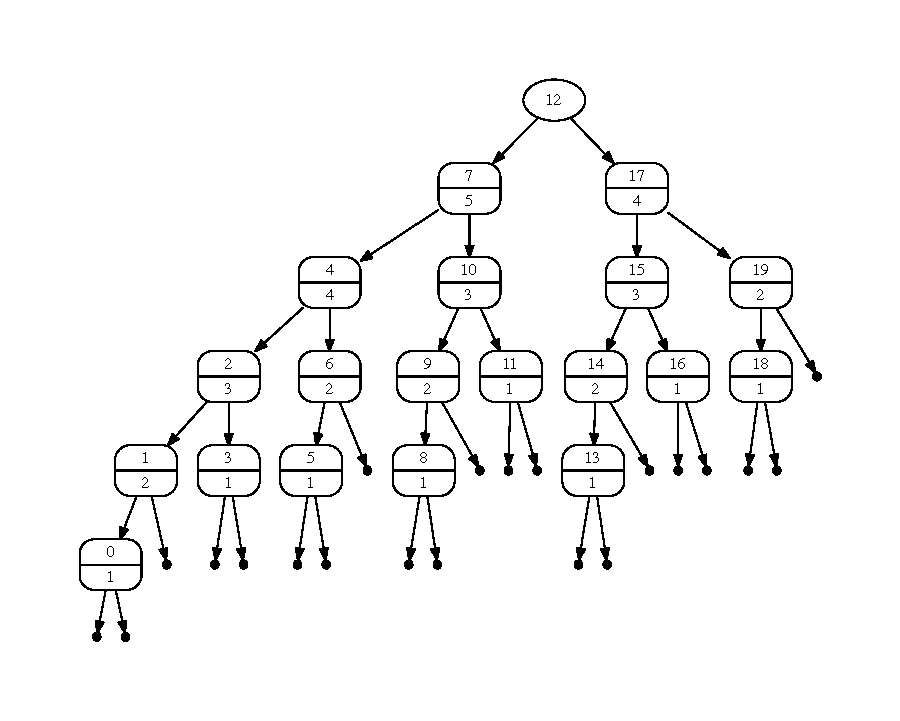
\epsfig{file=Abbildungen/avl}} 
  \caption{An AVL tree of height 6 that is as slim as possible.}
  \label{fig:avl-worst-case}
\end{figure}

\subsection{Improvements}
In practice, 
\href{https://en.wikipedia.org/wiki/Red-black_trees}{red-black trees} 
are slightly faster than \textsc{AVL} trees.  Similar to
\textsc{AVL} trees, a  red-black tree
  is an ordered binary tree that is approximately balanced.  Nodes are either black or red.
The children of a red node have to be black.  In order to keep red-black trees approximately
balanced, a \blue{relaxed height} of a tree is defined.  Red nodes do not contribute to the relaxed
height of a tree.  The left and right subtree of every node of a red-black tree are required to have the same 
relaxed height.  A detailed and very readable exposition of red-black trees is given by Sedgewick
\cite{sedgewick:2011}.  Red-black trees have been invented by Leonidas L.~Guibas and 
\href{https://en.wikipedia.org/wiki/Robert_Sedgewick_(computer_scientist)}{Robert Sedgewick} \cite{guibas:78}.

\exercise
Instead of using AVL trees, another alternative to implement a map is to use 
\href{https://en.wikipedia.org/wiki/2-3_tree}{2-3 trees}.  
Below we describe a simplified version of these trees.  These trees do not store any values.  Hence, instead
of implementing maps, these trees implement sets. They are built using the following constructors:
\begin{enumerate}
\item $\texttt{Nil}$ is a 2-3 tree that represents the empty set.
\item $\texttt{Two}(l, k, r)$ is a 2-3 tree provided
      \begin{enumerate}[(a)]
      \item $l$ is a 2-3 tree,
      \item $k$ is a key,
      \item $r$ is a 2-3 tree,
      \item all keys stored in $l$ are less than k and all keys stored in $r$ are bigger than $k$,
            i.e.~we have
            \\[0.2cm]
            \hspace*{1.3cm}
            $l < k < r$.
      \item $l$ and $r$ have the same height.
      \end{enumerate}
      A node of the form  $\texttt{Two}(l, k, r)$ is called a \blue{2-node}.  Except for the fact
      that there is no value, a 2-node is
      interpreted in the same way as we have interpreted the term $\texttt{Node}(k, v, l, r)$.
\item $\texttt{Three}(l, k_1, m, k_2, r)$ is a 2-3 tree provided
      \begin{enumerate}[(a)]
      \item $l$, $m$, and $r$ are 2-3 trees,
      \item $k_1$ and $k_2$ are keys,
      \item $l < k_1 < m < k_2 < r$,
      \item $l$, $m$, and $r$ have the same height.
      \end{enumerate}
      A node of the form  $\texttt{Three}(l, k_1, m, k_2, r)$ is called a \blue{3-node}.
\end{enumerate}
In order to keep 2-3 trees balanced when inserting new keys, we use a fourth constructor of the form
\\[0.2cm]
\hspace*{1.3cm}
$\texttt{Four}(l,k_1,m_l, k_2, m_r, k_3, r)$.
\\[0.2cm]
A term of the form $\texttt{Four}(l,k_1,m_l, k_2, m_r, k_3, r)$ is a \blue{2-3-4} tree iff
\begin{enumerate}
\item $l$, $m_l$, $m_r$, and $r$ are 2-3 trees,
\item $k_1$, $k_2$, and $k_3$ are keys,
\item $l < k_1 < m_l < k_2 < m_r < k_3 < r$,
\item $l$, $m_l$, $m_r$, and $r$ all have the same height.
\end{enumerate}
Nodes of this form are called 4-nodes and the key $k_2$ is called the \blue{middle key}.
Trees containing 4-nodes are called \blue{2-3-4} trees.
When a new key is inserted into a 2-3 tree, the challenge is to keep the tree balanced.  The easiest
case is the case where the tree has the form
\\[0.2cm]
\hspace*{1.3cm}
$\texttt{Two}(\texttt{Nil}, k, \texttt{Nil})$.
\\[0.2cm]
In this case, the 2-node is converted into a 3-node.  If the tree has the form 
\\[0.2cm]
\hspace*{1.3cm}
$\texttt{Three}(\texttt{Nil}, k_1, \texttt{Nil}, k_2, \texttt{Nil})$,
\\[0.2cm]
the 3-node is temporarily transformed into a 4-node.  Next, the middle key of this node is lifted up
to its parent node.  For example, suppose we insert the key 3 into the tree
\\[0.2cm]
\hspace*{1.3cm}
$\texttt{Two}(\texttt{Two}(\texttt{Nil}, 1, \texttt{Nil}), 2, \texttt{Three}(\texttt{Nil}, 4, \texttt{Nil}, 5, \texttt{Nil}))$.
\\[0.2cm]
In this case, the key 3 needs to be inserted to the left of the key 4.  This yields the temporary tree 
\\[0.2cm]
\hspace*{1.3cm}
$\texttt{Two}(\texttt{Two}(\texttt{Nil}, 1, \texttt{Nil}), 2, \texttt{Four}(\texttt{Nil}, 3, \texttt{Nil}, 4, \texttt{Nil}, 5, \texttt{Nil}))$.
\\[0.2cm]
Since this is not a 2-3 tree, we need to lift the middle key 4 to its parent node.  This results in
the new tree
\\[-0.1cm]
\hspace*{1.3cm}
$\texttt{Three}(\texttt{Two}(\texttt{Nil}, 1, \texttt{Nil}), 2, \texttt{Two}(\texttt{Nil}, 3, \texttt{Nil}), 4, \texttt{Two}(\texttt{Nil}, 5, \texttt{Nil}))$.
\\[0.2cm]
This tree is a 2-3 tree.  In this example we have been lucky since the parent of the 4-node was
a 2 node and therefore we could transform it into a 3-node.  If the parent node instead is a 3-node,
it has to be transformed into a temporary 4-node.  Then, the middle key of this 4-node has to be
lifted up recursively to its parent.  
\begin{enumerate}[(a)]
\item Specify a method $t.\texttt{member}(k)$ that checks whether the key $k$ occurs in the 2-3 tree
      $t$.  You should use recursive equations to specify  $t.\texttt{member}(k)$.
\item Specify a method $t.\texttt{insert}(k)$ that inserts the key $k$ into the 2-3 tree
      $t$.  You should use three auxiliary functions to implement \texttt{insert}:
      \begin{enumerate}
      \item $t.\texttt{ins}(k)$ takes a 2-3 tree $t$ and a key $k$ and inserts the key $k$ into $t$.
            It returns a 2-3-4 tree that has at most one 4-node.  Unless the tree $t$ has a height of $1$, this
            4-node has to be a child of the root node.  The function \texttt{ins} is recursive and uses the
            function \texttt{restore} that is described next.
            Furthermore, the height of the tree $t.\mathtt{ins}(k)$ has to be the same as the height of the tree $t$.
      \item $t.\texttt{restore}()$ takes a 2-3-4 tree $t$ that has at most one 4-node, which has to be a child
            of the root.  It returns a 2-3-4 tree that has at most one 4-node.  This 4-node has to be the root node.
            Furthermore, the height of the tree $t.\mathtt{restore}()$ has to be the same as the height of the tree $t$.
      \item $t.\texttt{grow}()$ takes a 2-3-4 tree $t$ that has at most one 4-node, which has to be the root
            node of the tree.  It returns an equivalent 2-3 tree.
      \end{enumerate}
      Having defined these auxiliary functions, the function \texttt{insert} can then be computed as follows:
      \\[0.2cm]
      \hspace*{1.3cm}
      $t.\texttt{insert}(k) = t.\texttt{ins}(k).\texttt{restore}().\texttt{grow}()$.
\item Implement 2-3 trees in \textsl{Python}.
\item \textbf{Optional}: Specify a method $t.\texttt{delete}(k)$ that deletes the key $k$ in the tree $t$.

      In order to implement the function \texttt{delete}, it is necessary to define 1-2-3 trees.
      In addition to both 2-nodes and 3-nodes, these trees also have 1-nodes.  These nodes come into existence
      when a key is deleted from a 2-node:  Deleting the key $k$ from the node
      \\[0.2cm]
      \hspace*{1.3cm}
      $\texttt{Two}(\texttt{Nil}, k, \texttt{Nil})$
      \\[0.2cm]
      creates the 1-node $\texttt{One}(\texttt{Nil})$.
\end{enumerate}
Prof. Lyn Turbak has written a helpful
\href{http://www.cs.princeton.edu/~dpw/courses/cos326-12/ass/2-3-trees.pdf}{paper} describing 2-3 trees in more
depth.  This paper gives a graphical presentation of the \texttt{insert} and \texttt{delete} operations.

\paragraph{History:}
According to \cite{cormen:09}, 2-3 trees have been invented by
\href{https://en.wikipedia.org/wiki/John_Hopcroft}{John Hopcroft} in 1970.  John Hopcroft received the 1986
Turing Award. 



\section{Tries}
Often, the keys of a map are strings.  For example, when you search with 
\href{https://www.google.com}{\raisebox{-4pt}{
\epsfig{file=Abbildungen/google.eps, scale=0.1}}}, you are using
a string as a key to lookup information that is stored in a gigantic map provided by \blue{Google}.
As another example, in an electronic phone book the keys are names and therefore strings.  
There is a species of search trees that is particularly well adapted to the case that the keys are
strings.  These search trees are known as \href{https://en.wikipedia.org/?title=Trie}{tries}.  
The name is derived from the word
\blue{re\underline{trie}val}.  In order to be able to distinguish between \blue{tries} and
\blue{trees} we have to pronounce  \blue{trie}  so that it rhymes with \blue{pie}.   The data
structure of tries has been proposed 1959 by Ren\'e de la Briandais \cite{briandais:59}.

Tries are also trees, but in contrast to a binary tree where every node has two children, in a trie a
node can have as many children as there are characters in the alphabet that is used to represent the
strings.  In order to define tries formally we assume that the following is given:
\begin{itemize}
\item $\Sigma$ is finite set of \blue{characters}. $\Sigma$ is called the
      \blue{alphabet}. 
\item $\Sigma^*$ is the set of all \blue{strings} that are built from the characters of $\Sigma$.
      Formally, a string is just a list of characters.  If we have $w \in \Sigma^*$, then we write $w = cr$
      if $c$ is the first character of $w$ and if $r$ the string that remains if we remove the first
      character from $w$.
\item $\varepsilon$ denotes the empty string.
\item $\texttt{Value}$ is the set of all the values that can be associated with the keys.  
\end{itemize}
The set $\mathbb{T}$ of all tries is defined inductively using the constructor \\[0.2cm]
\hspace*{1.3cm} 
$\texttt{Node}: \texttt{Value} \times \texttt{List}(\Sigma) \times
\texttt{List}(\mathbb{T}) \rightarrow \mathbb{T}$. 
\\[0.2cm]
The inductive definition of the set $\mathbb{T}$ has only a single clause: If
\begin{enumerate}
\item $v \in \texttt{Value} \cup \{\Omega\}$,
\item $C = [c_1, \cdots, c_n] \in \texttt{List}(\Sigma)$ is a list of different characters of length
      $n$ and,
\item $T = [t_1, \cdots, t_n] \in \texttt{List}(\mathbb{T})$ is a list of  tries of the same length $n$, 
\end{enumerate}
then we have 
\\[0.2cm]
\hspace*{1.3cm}  $\texttt{Node}(v, C, T) \in \mathbb{T}$.  
\\[0.2cm]
As there is only one clause in this definition, you might ask how this inductive definition gets started.
The answer is that the base case of this inductive definition is the case where
$n=0$ since in that case the lists  $C$ and $T$ are both empty.

Next, we specify the function that is represented by a trie of the form 
\\[0.2cm]
\hspace*{1.3cm} 
$\texttt{Node}(v, [c_1, \cdots, c_n], [t_1, \cdots, t_n])$.
\\[0.2cm]
In order to do so, we specify a function
\\[0.2cm]
\hspace*{1.3cm} 
$\texttt{find}: \mathbb{T} \times \Sigma^* \rightarrow \texttt{Value} \cup \{ \Omega\}$
\\[0.2cm]
that takes a trie and a string.  For a trie $t$ and a string $s$, the expression $t.\texttt{find}(s)$ returns the
value that is associated with the key $s$ in $t$.  The expression
$\texttt{Node}(v,C,T).\texttt{find}(s)$ is defined by induction on the length of the  string $s$:
\begin{enumerate}
\item $\texttt{Node}(v, C, T).\texttt{find}(\varepsilon) = v$.

      The value associated with the empty string $\varepsilon$ is stored at the root of the trie.
\item $\texttt{Node}(v, [c_1, \cdots, c_n], [t_1, \cdots, t_n]).\texttt{find}(cr) = 
        \left\{
        \begin{array}{ll}
        t_1.\texttt{find}(r) & \mbox{if} \quad c = c_1 \mbox{;} \\
        \vdots &                                     \\
        t_i.\texttt{find}(r) & \mbox{if} \quad c = c_i \mbox{;} \\
        \vdots &                                     \\
        t_n.\texttt{find}(r) & \mbox{if} \quad c = c_n \mbox{;} \\[0.2cm]
        \Omega               & \mbox{if} \quad c \notin \{c_1,\cdots,c_n\} \mbox{.}         
        \end{array}
       \right.$

      The trie $\texttt{Node}(v, [c_1, \cdots, c_n], [t_1, \cdots, t_n])$ associates a value with
      the key $cr$ if the list $[c_1, \cdots, c_n]$ has a position $i$ such that $c$ equals $c_i$
      and, furthermore, the trie  $t_i$ associates a value with the key  $r$.
\end{enumerate}

\begin{figure}[!ht]
  \centering
  \framebox{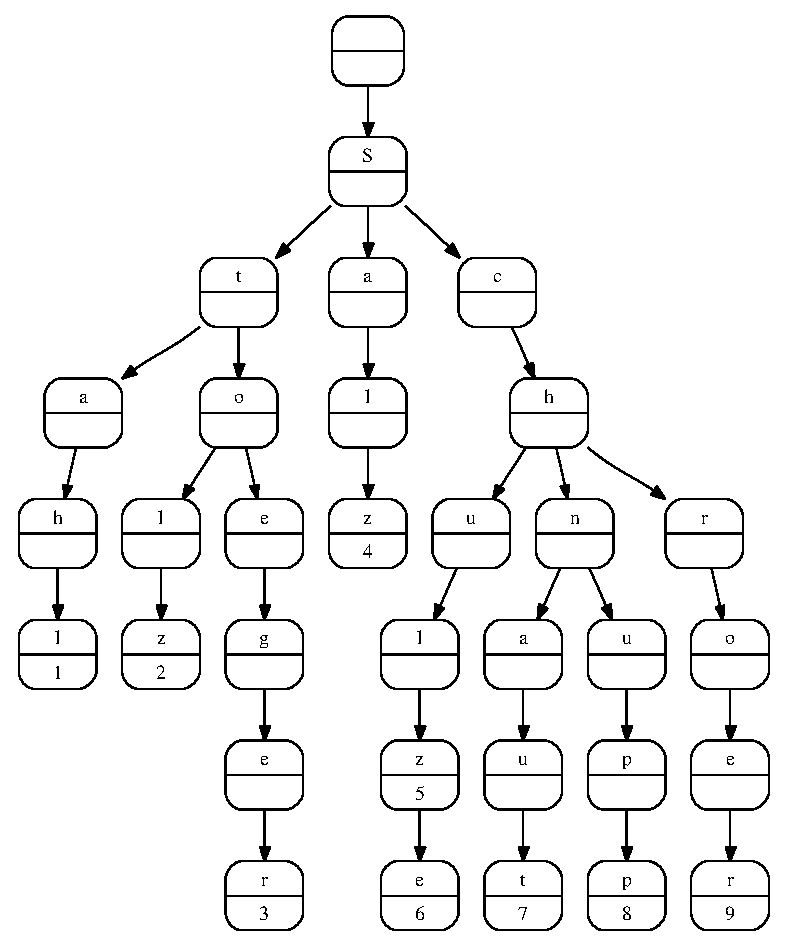
\epsfig{file=Abbildungen/trie}} 
  \caption{A trie storing some numbers.}
  \label{fig:trie}
\end{figure}

Graphically, tries are represented as trees.  Since it would be unwieldy to label the nodes of these
trees with the lists of characters corresponding to these nodes, we use a trick:  In order to
visualize a node of the form \\[0.2cm]
\hspace*{1.3cm} 
$\texttt{Node}(v, [c_1, \cdots, c_n], [t_1, \cdots, t_n])$ \\[0.2cm]
we draw a oval.  This oval is split into two parts by a horizontal line.
If the value  $v$ that is stored in this node is different from $\Omega$, then the value $v$ is
written in the lower part of the oval.  The label that we put in the upper half of the oval
depends on the parent of the node.  We will explain how this label is computed in a moment.
The node itself has $n$ different children.  These $n$ children are the tries
$t_1$, $\cdots$, $t_n$.  The node at the root of the trie $t_i$ is labelled with the character $c_i$,
i.e.~the oval that represents this node carries the label $c_i$ in its upper half.

In order to clarify these ideas, Figure  \ref{fig:trie} on page \pageref{fig:trie} shows a trie
mapping some strings to numbers.  The mapping depicted in this tree can be written as a functional
relation: 
\\[0.2cm]
\hspace*{1.3cm} $ \bigl\{ \langle \textrm{``Stahl''},   1  \rangle, \langle \textrm{``Stolz''},     2  \rangle, \langle \textrm{``Stoeger''},   3  \rangle, 
             \langle \textrm{``Salz''},      4  \rangle, \langle \textrm{``Schulz''},    5  \rangle$, \\[0.2cm]
\hspace*{1.5cm} $\langle \textrm{``Schulze''},   6  \rangle, \langle \textrm{``Schnaut''},   7  \rangle, 
  \langle \textrm{``Schnupp''},   8  \rangle, 
  \langle \textrm{``Schroer''},   9  \rangle\}$. \\[0.2cm]
Since the node at the root has no parent, the upper half of  the oval representing the root is
always empty.  In the example shown in Figure \ref{fig:trie}, the lower half of this oval is also empty
because the trie doesn't associate a value with the empty string.  In this example, the root node corresponds
to the term  
\\[0.2cm]
\hspace*{1.3cm}
 $\texttt{Node}(\Omega,[\textrm{`S'}], [t])$. 
\\[0.2cm]
Here,  $t$ denotes the trie that is labelled with the character  ``S'' at its root.
This trie can then be represented by the term  \\[0.2cm]
\hspace*{1.3cm} 
$\texttt{Node}(\Omega,[\textrm{`t'},\textrm{`a'},\textrm{`c'}], [t_1, t_2, t_3])$. \\[0.2cm]
This trie has three children that are labelled with the characters  ``t'', ``a'', and ``c''.

\subsection{Insertion in Tries}
Next, we present formul\ae\ that describe how new values can be inserted into existing tries,
i.e.~we specify the method $\texttt{insert}$.  The signature of $\texttt{insert}$ is given as follows:
\\[0.2cm]
\hspace*{1.3cm}
$\texttt{insert}: \mathbb{T} \times \Sigma^* \times \texttt{Value} \rightarrow \mathbb{T}$.
\\[0.2cm]
The result of evaluating \\[0.2cm]
\hspace*{1.3cm} 
$\texttt{Node}(v_1, [c_1, \cdots, c_n], [t_1, \cdots, t_n]).\texttt{insert}(w, v_2)$
\\[0.2cm]
for a string $w\in \Sigma^*$ and a value $v_2 \in \texttt{Value}$ is defined by induction on the
length of $w$.
\begin{enumerate}
\item $\texttt{Node}(v_1,L,T).\texttt{insert}(\varepsilon, v_2) = \texttt{Node}(v_2,L,T)$,
  
      If a new value $v_2$ is associated with the empty string $\varepsilon$, then the old value
      $v_1$, which had been stored at the root before, is overwritten.
\item $\texttt{Node}\bigl(v_1,[c_1,\cdots,c_i,\cdots,c_n], [t_1,\cdots,t_i,\cdots,t_n]\bigr).\texttt{insert}(c_ir,v_2) =$ \\[0.2cm]
      \hspace*{1.3cm}  
      $\texttt{Node}\bigl(v_1,[c_1,\cdots,c_i,\cdots,c_n], [t_1,\cdots,t_i.\texttt{insert}(r,v_2),\cdots,t_n]\bigr)$.

      In order to associate a value $v_2$ with the string $c_ir$ in the trie
      \\[0.2cm]
      \hspace*{1.3cm}
      $\texttt{Node}\bigl(v_1,[c_1,\cdots,c_i,\cdots,c_n], [t_1,\cdots,t_i,\cdots,t_n]\bigr)$ 
      \\[0.2cm]
      we have to recursively associate the value $v_2$ with the string $r$ in the trie $t_i$.
\item $c \not\in\{c_1,\cdots,c_n\} \;\rightarrow\;\texttt{Node}\bigl(v_1,[c_1,\cdots,c_n], [t_1,\cdots,t_n]\bigr).\texttt{insert}(cr,v_2) =$ \\[0.2cm]
      \hspace*{1.3cm}  
      $\texttt{Node}\bigl(v_1,[c_1,\cdots,c_n,c], [t_1,\cdots,t_n,\texttt{Node}(\Omega,[],[]).\texttt{insert}(r,v_2)]\bigr)$.
      
      If we want to associate a value $v$ with the key $cr$ in the trie
      $\texttt{Node}\bigl(v_1,[c_1,\cdots,c_n], [t_1,\cdots,t_n]\bigr)$ then, if the character $c$
      does not occur in the list $[c_1,\cdots,c_n]$, we first have to create a new empty trie.
      This trie has the form \\[0.2cm]
      \hspace*{1.3cm} $\texttt{Node}(\Omega, [], [])$. \\[0.2cm]
      Next, we associate the value $v_2$ with the key $r$ in this empty trie.  Finally,
      we append the character $c$ to the end of the list $[c_1,\cdots,c_n]$ and append the trie
        \\[0.2cm] 
      \hspace*{1.3cm}
      $\texttt{Node}(\Omega, [], []).\texttt{insert}(r,v_2)$ 
      \\[0.2cm]
      to the end of the list $[t_1,\cdots,t_n]$.
\end{enumerate}

\subsection{Deletion in Tries}
Finally, we present formul\ae\ that specify how a key can be deleted from a trie.
To this end, we define the auxiliary function
\\[0.2cm]
\hspace*{1.3cm} 
$\texttt{isEmpty}: \mathbb{T} \rightarrow \mathbb{B}$.
\\[0.2cm]
For a trie $t$, we have $t.\texttt{isEmpty}() = \texttt{True}$ if and only if the trie $t$ does not
store any key.  The following formula specifies the function $\texttt{isEmpty}$:
\\[0.2cm]
\hspace*{1.3cm}
$\texttt{Node}(v, L, T).\texttt{isEmpty}() = \mathtt{True} \Leftrightarrow v = \Omega \wedge L = []$
\\[0.2cm]
Now, we can specify the method
\\[0.2cm]
\hspace*{1.3cm}
$\texttt{delete}: \mathbb{T} \times \Sigma^* \rightarrow \mathbb{T}$.
\\[0.2cm]
For a trie  $t \in \mathbb{T}$ and a string $w \in \Sigma^*$ the value 
 \\[0.2cm]
\hspace*{1.3cm} 
$t.\texttt{delete}(w)$
\\[0.2cm]
is defined by induction on the length of  $w$.
\begin{enumerate}
\item $\texttt{Node}(v,C,T).\texttt{delete}(\varepsilon) = \texttt{Node}(\Omega,C,T)$

      The value that is associated with the empty  string $\varepsilon$ is stored at the root of the
      trie where is can be deleted without further ado.
\item $\begin{array}[t]{ll}
       t_i.\texttt{delete}(r).\texttt{isEmpty}()   & \rightarrow \\
       \texttt{Node}(v, [c_1,\cdots,c_i,\cdots,c_n],[t_1,\cdots,t_i,\cdots,t_n]).\texttt{delete}(c_ir) 
       & = \\
       \qquad 
       \texttt{Node}(v, [c_1,\cdots,c_{i-1},c_{i+1},\cdots,c_n],[t_1,\cdots,t_{i-1},t_{i+1},\cdots,t_n]).
       \end{array}
       $

       If  the key that is to be deleted starts with the character $c_i$ and if deletion of  the key
       $r$ in the $i$th  trie $t_i$ yields an empty
       trie, then both the $i$th character $c_i$ and the $i$th trie $t_i$ are deleted.
\item $\begin{array}[t]{ll}
       \neg t_i.\texttt{delete}(r).\texttt{isEmpty}()   & \rightarrow \\
       \texttt{Node}(v, [c_1,\cdots,c_i,\cdots,c_n],[t_1,\cdots,t_i,\cdots,t_n]).\texttt{delete}(c_ir) 
       & = \\
       \qquad \texttt{Node}(v, [c_1,\cdots,c_i,\cdots,c_n],[t_1,\cdots,t_i.\texttt{delete}(r),\cdots,t_n]).
       \end{array}
       $

       If  the key that is to be deleted starts with the character $c_i$ and if deletion of  the key
       $r$ in the $i$th  trie $t_i$ yields a non-empty trie, then the key $r$ has to be deleted recursively
       in the trie $t_i$.
\item $c \notin C \rightarrow \texttt{Node}(v, C, T).\texttt{delete}(cr) =
       \texttt{Node}(v, C, T)$. 
       
       If  the key that is to be deleted starts with the character $c$ and $c$ does not occur in
       the list of characters $C$, then the trie does not contain the key $cr$ and therefore there
       is nothing to do:  The trie is left unchanged.
\end{enumerate}

\subsection{Complexity}
It is straightforward to see that the complexity of looking up the value associated with a string
$s$ of length $k$ is $\Oh(k)$.  In particular, it is independent on the number of strings $n$.  As
it is obvious that we have to check all $k$ characters of the string $s$, this bound cannot be
improved.   Another advantage of tries is the fact that they use very little storage to store the
keys because common prefixes are only stored once. 

\subsection{Implementing Tries in \textsl{Python}}
\begin{figure}[!ht]
\centering
\begin{minted}[ frame         = lines, 
                  framesep      = 0.3cm, 
                  firstnumber   = 1,
                  bgcolor = sepia,
                  numbers       = left,
                  numbersep     = -0.2cm,
                  xleftmargin   = 0.8cm,
                  xrightmargin  = 0.8cm,
                ]{python3}
    class Trie(): 
        def __init__(self):
            self.mValue  = None
            self.mChars  = []
            self.mTries  = []
\end{minted}
\vspace*{-0.3cm}
\caption{The constructor of the class \texttt{Trie}.}
\label{fig:trie.ipython-outline}
\end{figure}

\noindent
We proceed to discuss the implementation of tries.  Figure \ref{fig:trie.ipython-outline} shows the
definition of the class \texttt{Trie} and its constructor.  This class supports three member variables.  In order to
understand these member variables, remember that a trie has the form
\\[0.2cm]
\hspace*{1.3cm}
$\texttt{Node}(v, C, T)$
\\[0.2cm]
where $v$ is the value stored at the root, $C$ is the list of characters, and $T$ is a list of
tries.  Therefore, the member variables have the following semantics:
\begin{enumerate}
\item $\texttt{mValue}$ represent the value $v$ stored at the root of this trie,  
\item $\texttt{mChars}$ represent the list  $C$ of characters.  If there is a string $cr$ such that
      the trie stores a value associated with this string, then the character $c$ will be an element of
      the list $C$.
\item $\texttt{mTries}$ represent the list of subtries $T$.  
\end{enumerate}
The class $\texttt{Trie}$ implements the abstract data type $\texttt{map}$ and therefore provides the
methods $\texttt{find}$, $\texttt{insert}$, and $\texttt{delete}$.  Furthermore, the method
$\texttt{isEmpty}$ is an auxiliary method that is needed in the implementation of the method 
$\texttt{delete}$.  This method checks whether the given trie corresponds to the empty map.  The
implementation of all these methods is given below. 

\begin{figure}[!ht]
\centering
\begin{minted}[ frame         = lines, 
                  framesep      = 0.3cm, 
                  firstnumber   = 1,
                  bgcolor = sepia,
                  numbers       = left,
                  numbersep     = -0.2cm,
                  xleftmargin   = 0.8cm,
                  xrightmargin  = 0.8cm,
                ]{python3}
    def find(self, s):
        if s == '':
            return self.mValue
        c, r = s[0], s[1:]
        for i, ci in enumerate(self.mChars):
            if c == ci:
                return self.mTries[i].find(r)
\end{minted}
\vspace*{-0.3cm}
\caption{Implementation of $\texttt{find}$ for tries.}
\label{fig:trie.ipython-find}
\end{figure}

The method $\texttt{find}$ takes a string $s$ as its sole argument and checks whether the given trie
contains a value associated with the string $s$.  Essentially, the are two cases:
\begin{enumerate}
\item If $s$ is the empty string, the value associated with $s$ is stored in the member variable
      $\texttt{mValue}$ at the root of this trie.
\item Otherwise, $s$ can be written as $s = cr$ where $c$ is the first character of $s$ while $r$
      consists of the remaining characters.  In order to check whether the trie has a value stored
      for $s$ we first have to check whether there is an index $i$ such that $\texttt{mChars}[i]$ is
      equal to $c$.  If this is the case, the subtrie $\texttt{mTries}[i]$ contains the value
      associated with $s$.  Then, we have to invoke $\texttt{find}$ recursively on this subtrie.

      If the loop in line 5 does not find the character $c$ in the list $\texttt{mChars}$, then the method
      $\texttt{find}$ will just return the undefined value $\texttt{None}$.  In \textsl{Python} this happens
      automatically when a function ends without explicitly returning a value.
\end{enumerate}


\begin{figure}[!ht]
\centering
\begin{minted}[ frame         = lines, 
                  framesep      = 0.3cm, 
                  firstnumber   = 1,
                  bgcolor = sepia,
                  numbers       = left,
                  numbersep     = -0.2cm,
                  xleftmargin   = 0.8cm,
                  xrightmargin  = 0.8cm,
                ]{python3}
    def insert(self, s, v):
        if s == '':
            self.mValue = v
            return
        c, r = s[0], s[1:]
        for i, ci in enumerate(self.mChars):
            if c == ci:
                self.mTries[i].insert(r, v)
                return
        t = Trie()
        t.insert(r, v)
        t.mParent = c # necessary for visualization
        self.mChars.append(c)
        self.mTries.append(t)
\end{minted}
\vspace*{-0.3cm}
\caption{Implementation of $\texttt{insert}$ for tries.}
\label{fig:trie.ipython-insert}
\end{figure}


The method $\texttt{insert}$ takes a string $s$ and an associated value $v$ that is to be inserted
into the given trie.  The implementation of $\texttt{insert}$ works somewhat similar to the
implementation of $\texttt{find}$.
\begin{enumerate}
\item If the string $s$ is empty, then the value $v$ has to be positioned at the root of this trie.
      Hence we just set $\texttt{mValue}$ to $v$ and return.
\item Otherwise, $s$ can be written as $cr$ where $c$ is the first character of $s$ while $r$
      consists of the remaining characters.  In this case, we need to check whether the list
      $\texttt{mChars}$ already contains the character $c$ or not.
      \begin{enumerate}
      \item If $c$ is the $i$-th character of $\texttt{mChars}$, then we have to insert the value $v$
            in the trie $\texttt{mTries}[i]$.  
      \item If $c$ does not occur in $\texttt{mChars}$, things are straightforward: We create a new
            empty trie and insert $v$ into this trie.  Next, we append the character $c$ to
            $\texttt{mChars}$ and simultaneously append the newly created trie that contains $v$ to
            $\texttt{mTries}$. 
      \end{enumerate}
\end{enumerate}

\begin{figure}[!ht]
\centering
\begin{minted}[ frame         = lines, 
                  framesep      = 0.3cm, 
                  firstnumber   = 1,
                  bgcolor = sepia,
                  numbers       = left,
                  numbersep     = -0.2cm,
                  xleftmargin   = 0.0cm,
                  xrightmargin  = 0.0cm,
                ]{python3}
    def delete(self, s):
        if s == '':
            self.mValue = None
            return
        c, r = s[0], s[1:]
        for i, ci in enumerate(self.mChars):
            if c == ci:
                self.mTries[i].delete(r)
                if self.mTries[i].isEmpty():
                    self.mChars.pop(i)
                    self.mTries.pop(i)
                return
\end{minted}
\vspace*{-0.3cm}
\caption{Implementation of $\texttt{delete}$ for tries.}
\label{fig:trie.ipython-delete}
\end{figure}

The method $\texttt{delete}$ takes a string $s$ and, provided there is a value associated with $s$, this
value is deleted.
\begin{enumerate}
\item If the string $s$ is empty, the value associated with $s$ is stored at the root of this trie.
      In order to remove this value, the variable $\texttt{mValue}$ is set to $\texttt{None}$, which represents
      the undefined value $\Omega$ in \textsl{Python}.
\item Otherwise, $s$ can be written as $cr$ where $c$ is the first character of $s$ while $r$
      consists of the remaining characters.  In this case, we need to check whether the list
      $\texttt{mChars}$ contains the character $c$ or not.
 
      If $c$ is the $i$-th character of $\texttt{mChars}$, then we have to recursively
      delete the value associated with $r$ in the trie $\texttt{mTries}[i]$.  
      After this deletion, the subtrie  $\texttt{mTries}[i]$ might well be empty.  In this case,
      we remove the $i$-th character form $\texttt{mChars}$ and also remove the $i$-th trie from the list
      $\texttt{mTries}$.  This is done with the help of the function $\texttt{pop}$.
      Given a list $L$ and an integer $i$, the statement $L.\texttt{pop}(i)$ removes the $i$-th element from
      the list $L$.
\end{enumerate}

\begin{figure}[!ht]
\centering
\begin{minted}[ frame         = lines, 
                  framesep      = 0.3cm, 
                  firstnumber   = 1,
                  bgcolor = sepia,
                  numbers       = left,
                  numbersep     = -0.2cm,
                  xleftmargin   = 0.8cm,
                  xrightmargin  = 0.8cm,
                ]{python3}
    def isEmpty(self):
        return self.mValue == None and self.mChars == []
\end{minted}
\vspace*{-0.3cm}
\caption{Implementation of $\texttt{isEmpty}$ for tries.}
\label{fig:trie.ipython-isEmpty}
\end{figure}

In order to check whether a given trie is empty it suffices to check that no value is stored at the root
and that the list $\texttt{mChars}$ is empty, since then the list $\texttt{mTries}$ will also be empty.  Hence,
there is no need to recursively check whether all tries in $\texttt{mTries}$ are empty.  
The implementation is shown in Figure \ref{fig:trie.ipython-isEmpty}.

\exercise
(\textbf{Binary Tries})  Let us assume that our alphabet is the binary alphabet, i.e.~the alphabet
only contains the two digits $0$ and $1$.  Therefore we have $\Sigma = \{0,1\}$.  Every natural
number can be regarded as a string from the alphabet $\Sigma$, so that numbers are effectively
elements of $\Sigma^*$.  The set $\BT$ of \blue{binary tries} is defined by induction:
\begin{enumerate}
\item $\texttt{Nil} \in \BT$.
\item $\texttt{Bin}(v,l,r) \in \BT$ provided that
      \begin{enumerate}
      \item $v \in \texttt{Value} \cup \{\Omega\}$ \quad and
      \item $l,r \in \BT$.
      \end{enumerate}
\end{enumerate}
The semantics of binary tries is fixed by defining the function
\\[0.2cm]
\hspace*{1.3cm}
$\texttt{find}: \BT \times \mathbb{N} \rightarrow \texttt{Value} \cup \{ \Omega \}$.
\\[0.2cm]
Given a binary trie $b$ and a natural number $n$, the expression
\\[0.2cm]
\hspace*{1.3cm}
$b.\texttt{find}(n)$ 
\\[0.2cm]
returns the value in $b$ that is associated with the number $n$.  If there is no value associated
with $b$, then the expression evaluates to $\Omega$.  Formally, the value of the expression
 $b.\texttt{find}(n)$ is defined by induction on $b$.  The induction step requires a side induction
 with respect to the natural number $n$.
\begin{enumerate}
\item $\texttt{Nil}.\texttt{find}(n) = \Omega$,

      since the empty trie doesn't store any values.
\item $\texttt{Bin}(v,l,r).\texttt{find}(0) = v$,

      because $0$ is interpreted as the empty string $\varepsilon$.
\item $n \not= 0 \rightarrow \texttt{Bin}(v,l,r).\texttt{find}(2\cdot n) = l.\texttt{find}(n)$,

      because if a number is represented in binary, then the last bit of every even number is zero
      and zero chooses the left subtree.
\item $\texttt{Bin}(v,l,r).\texttt{find}(2 \cdot n + 1) = r.\texttt{find}(n)$,

      because if a number is represented in binary, then the last bit of every odd number is 1 and 
      1 is associated with the right subtree.
\end{enumerate}
Solve the following exercises:
\begin{enumerate}[(a)]
\item Provide equations that specify the methods $\texttt{insert}$ and $\texttt{delete}$ in a binary trie.
      When specifying delete you should take care that empty binary tries are reduced to
      $\texttt{Nil}$.

      \textbf{Hint}:  It might be helpful to provide an auxiliary method that simplifies those binary tries
      that are empty. 
\item Implement binary tries in \textsl{Python}.
\item Test your implementation with a nontrivial example.
\end{enumerate}
\textbf{Remark}: Binary tries are known as \blue{digital search trees}.  \eox

\section{Hash Tables}
It is very simple to implement a function of the form \\[0.2cm]
\hspace*{1.3cm} $f: \texttt{Key} \rightarrow \texttt{Value}$ \\[0.2cm]
provided the set $\texttt{Key}$ is a set of natural numbers of the form  \\[0.2cm]
\hspace*{1.3cm} $\texttt{Key} = \{ 0, 1, 2, \cdots, n \}$. \\[0.2cm]
In this case, we can implement the function $f$ via an array of size $n$.
Figure \ref{fig:map-array.ipython} shows how a map can be realized in this case.

\begin{figure}[!ht]
\centering
\begin{minted}[ frame         = lines, 
                  framesep      = 0.3cm, 
                  firstnumber   = 1,
                  bgcolor = sepia,
                  numbers       = left,
                  numbersep     = -0.2cm,
                  xleftmargin   = 0.8cm,
                  xrightmargin  = 0.8cm,
                ]{python3}
    class ArrayMap:
        def __init__(self, n):
            self.mArray = [None] * (n + 1)
            
        def find(self, k):
            return self.mArray[k]
        
        def insert(self, k, v):
            self.mArray[k] = v
    
        def delete(self, k):
            self.mArray[k] = None
\end{minted}
\vspace*{-0.3cm}
\caption{Implementing a map as an array.}
\label{fig:map-array.ipython}
\end{figure}

\begin{enumerate}
\item The constructor takes a second argument $n$.  This argument specifies the
      maximum size that a key is allowed to have.  Therefore, it is assumed that
      the keys are elements of the set $\{0,1, \cdots, n\}$.
\item The member variable maintained by the class \texttt{ArrayMap} is the array \texttt{mArray}.
      Initially, all entries of this array are \texttt{None}.
\item The method \texttt{find} looks up the value stored at the index $k$.
\item The method \texttt{insert} stores the value $v$ at the index $k$.
\item The method \texttt{delete} removes the value stored at the index $k$ by overwriting it with the undefined
      value. 
\end{enumerate}
If the domain $D := \texttt{dom}(f)$ of the function $f$ is not a set of the form $\{0,1, \cdots, n\}$, 
then we can instead try to find a one-to-one mapping of $D$ onto a set of the form $\{0,1,\cdots,n\}$.
Let us explain the idea with a simple example:  Suppose we want to implement an digital
telephone book.
To simplify things, let us assume first that all the names stored in our telephone dictionary
have a length of 8 characters.  To achieve this, names that are shorter than eight characters
are filled with spaces and if a name has more than eight characters, all characters after the
eighth character are dropped.

Next, every name is translated into an index.  In order to do so, the different
characters are interpreted as digits in a system where the digits can take values starting
from 0 up to the value 26.
Let us assume that the function  $\texttt{ord}$ takes a character from the set
\\[0.2cm]
\hspace*{1.3cm}
$\Sigma = \{ \texttt{' '}, \texttt{'a'}, \texttt{'b'}, \texttt{'c'}, \cdots, \texttt{'x'}, \texttt{'y'}, \texttt{'z'} \}$ 
\\[0.2cm]
and assigns a number from the set $\{0,\cdots,26\}$ to this character, i.e.~we have \\[0.2cm]
\hspace*{1.3cm} 
$\texttt{ord}: \{ \texttt{' '}, \texttt{'a'}, \texttt{'b'}, \texttt{'c'}, \cdots, \texttt{'x'}, \texttt{'y'},
\texttt{'z'} \} \rightarrow \{0,\cdots, 26\}$, \quad where
\\[0.2cm]
\hspace*{1.3cm}
$\texttt{ord}(\texttt{' '}) := 0$, \quad
$\texttt{ord}(\texttt{'a'}) := 1$, \quad
$\texttt{ord}(\texttt{'b'}) := 2$, \quad $\cdots$, \quad
$\texttt{ord}(\texttt{'z'}) := 26$.
\\[0.2cm]
Then, the value of the string  $w = c_0c_1\cdots c_7$ can be computed by the function \\[0.2cm]
\hspace*{1.3cm} 
$\texttt{code}: \Sigma^* \rightarrow \mathbb{N}$ \\[0.2cm]
as follows: \\[0.2cm]
\hspace*{1.3cm} 
$\ds \texttt{code}(c_0c_1\cdots c_7) = \sum\limits_{i=0}^7 \texttt{ord}(c_i) \cdot 27^i$.
\\[0.2cm]
The function $\texttt{code}$ maps the set of all non-empty strings with at most eight characters in a
one-to-one way to the set of numbers $\{0,1,\cdots, 282,429,536,480 \}$.


\begin{figure}[!ht]
  \centering
  \framebox{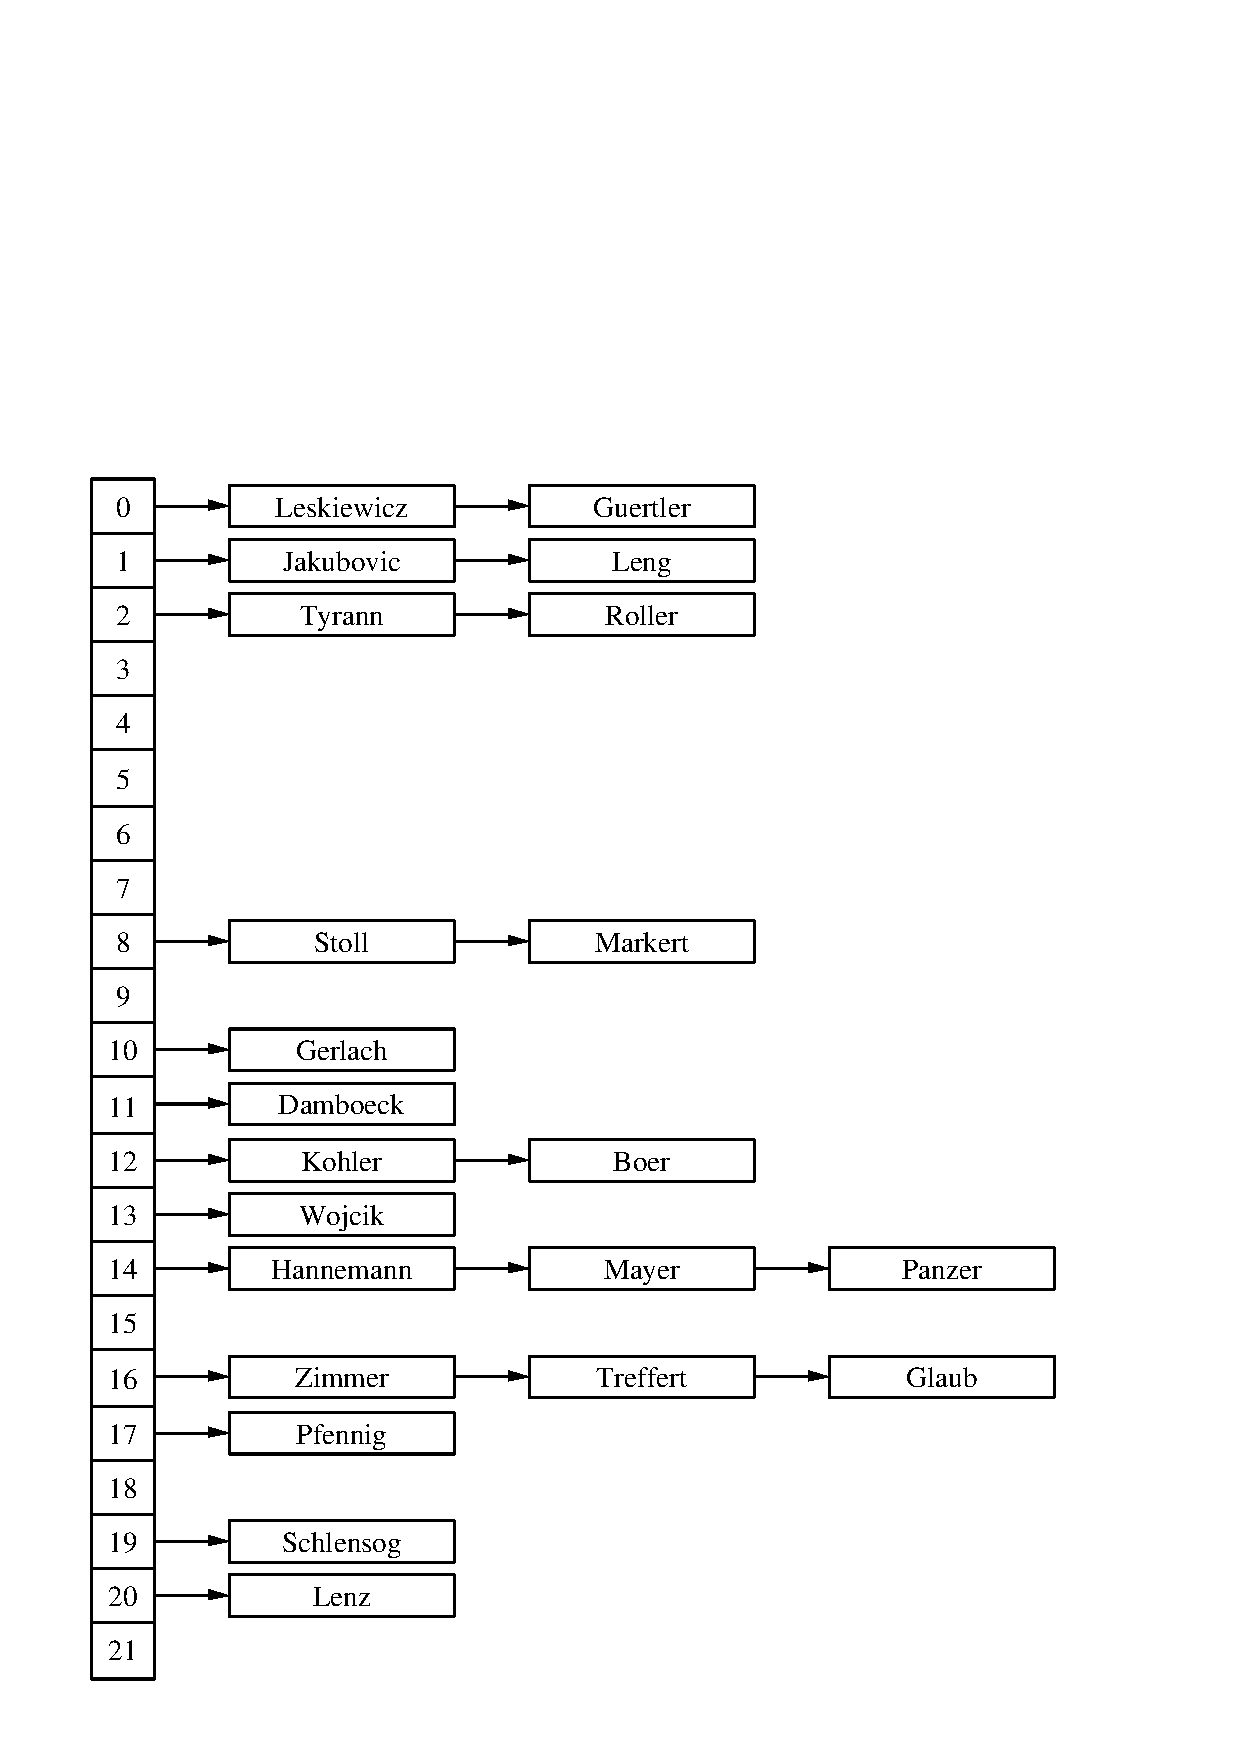
\epsfig{file=Abbildungen/hash-table,scale=0.6}} 
  \caption{A hash table.}
  \label{fig:hash-example}
\end{figure}

\noindent
Unfortunately, this naive implementation has several problems: 
\begin{enumerate}
\item The array needed to store the telephone dictionary has a size of 
      \\[0.2cm]
      \hspace*{1.3cm}
      $\ds 1 + \sum\limits_{i=0}^7 26 \cdot 27^i = 1 + 26 \cdot \frac{27^{7+1} - 1}{27 - 1} = 1 + 27^8 = 282,429,536,482$ 
      \\[0.2cm]
      entries.  If every entry needs 8 bytes, we would need more than two terabyte to store this array.
\item If two names happen to differ only after their eighth character, then we would not be able to
      store both of these names as we would not be able to distinguish between them.
\end{enumerate}
These problems can be solved as follows:
\begin{enumerate}
\item We have to change the function  $\texttt{code}$ so that the result of this function is always
      less than or equal to some given number $\texttt{size}$.  Here, the number $\texttt{size}$ specifies
      the number of entries of the array that we intend to use.  This number will be in the same
      order of magnitude as the number of key-value pairs that we want to store in our dictionary.

      There is a simple way to adapt the function  $\texttt{code}$ so that its result is never bigger
      than a given number $\texttt{size}$: If we define $\texttt{code}$ as
      \\[0.2cm]
      \hspace*{1.3cm} 
      $\ds\texttt{code}(c_0c_1\cdots c_n) = \left(\sum\limits_{i=0}^n \texttt{ord}(c_i) \cdot
        27^i\right) \;\texttt{\%}\; \texttt{size}$,
      \\[0.2cm]
      then we will always have $1 \leq \texttt{code}(c_0c_1\cdots c_n) < \texttt{size}$.  In order to
      prevent overflow when computing the numbers $27^i$ we can use the following mathematical facts:
      \\[0.2cm]
      \hspace*{1.3cm}
      $(a + b)   \mod n = \bigl(a + (b \mod n)\bigr) \mod n$ \quad and \quad
      $(a \cdot b) \mod n = \bigl(a \cdot (b \mod n)\bigr) \mod n$.
      \\[0.2cm]
      Then we can  define the partial sum $s_k$ for
      $k=n,n-1,\cdots,1,0$ by backward induction: 
      \begin{enumerate}
      \item $s_n = \texttt{ord}(c_n)$,
      \item $s_{k} = \bigl(\texttt{ord}(c_{k}) + s_{k+1} \cdot 27 \bigr) \;\texttt{\%}\; \texttt{size}$.
      \end{enumerate}
      It can be shown that
      \\[0.2cm]
      \hspace*{1.3cm} 
      $\ds s_0 = \left(\sum\limits_{i=0}^n \texttt{ord}(c_i) \cdot 27^i\right) \;\texttt{\%}\; \texttt{size}$.
\item Rather than storing the values associated with the keys in an array, the values are now stored
      in \blue{linked lists} that contain key-value pairs.  The array itself only stores pointers to these
      linked list. 
      
      The reason we have to use linked lists is the fact that different keys may be mapped to the
      same index.  Hence, we can no longer store the values directly in the array.  Instead,
      the values of all keys that map to the same index are stored in a
      linked list of key-value pairs.  These linked lists are then stored in the array.  As long as
      these lists contain only a few entries, the look-up of a key is still fast: Given a key $k$,
      we first compute 
      \\[0.2cm]
      \hspace*{1.3cm}
      $\texttt{idx} = \texttt{code}(k)$.
      \\[0.2cm]
      Then, $\texttt{array}[\texttt{idx}]$ returns a linked list containing a pair of the form $\langle k, v \rangle$.
      In order to find the value associated with the key $k$ we have to search this list for the key
      $k$.
\end{enumerate}

\subsection{Computing the Hash Function efficiently}
In this section we discuss how to compute the function 
\\[0.2cm]
\hspace*{1.3cm}
$\texttt{hash\_code}:\Sigma^* \rightarrow \mathbb{N}$
\\[0.2cm]
that takes a string $s$ and returns a natural number less than some predefined size $n$.
Given an \textsc{Ascii} string $s = c_0 c_1 c_2 \cdots c_{k-1}$ of length $k$ this function is defined as
\begin{equation}
  \texttt{hash\_code}(c_0c_1\cdots c_{k-1}, n) = \left(\sum\limits_{i=0}^k \texttt{ord}(c_i) \cdot 128^i\right) \mmod n.
  \label{eq:hash1}
\end{equation}
However, a naive implementation of equation (\ref{eq:hash1}) is inefficient because the computation of $128^i$
produces very big numbers.  In the programming language \texttt{C}, computing $128^{k-1}$ causes an overflow for a
string that has more than five characters.  In \textsl{Python}, integers are only bounded by the size of the
available memory and therefore overflow ist not a problem.  However, a computation
involving numbers with hundreds of places is considerably slower than a computation that uses numbers that fit
into a single memory word. Hence we should try to reorganize the computation that happens in equation
(\ref{eq:hash1}).  This should be possible as the final result of $\texttt{hash\_code}(c_0c_1\cdots c_{k-1}, n)$
is bounded by $n$.  In order to be able to reorganize this computation we need to discuss
\href{https://en.wikipedia.org/wiki/Euclidean_division}{Euclidean division}.

\begin{Theorem}[Euclidean Division]
  Given two natural numbers $a, n \in \mathbb{N}$ such that $n > 0$, there exist \textbf{unique} natural numbers 
  $q$ and $r$ such that:
  \begin{enumerate}[(a)]
  \item $a = q \cdot n + r$ \quad and
  \item $0 \leq r < n$.
  \end{enumerate}
  The number $q$ is called the \blue{quotient} of $a$ divided $n$ and denoted as $a \;\texttt{//}\; n$, while
  $r$ is called the \blue{remainder} of $a$ divided by $n$ and denoted as $a \mmod n$.  \eox
\end{Theorem}

A proof of this theorem can be given by writing a program that computes $a \;\texttt{//}\; n$ by successively subtracting
$n$ from $a$ as long as the result of the subtraction is non-negative.  Then $a \;\texttt{//}\; n$ is the number of times $n$ can be
subtracted from $a$.  Figure \ref{fig:Division-Naive.ipynb} shows an implementation of this idea.

\begin{figure}[!ht]
\centering
\begin{minted}[ frame         = lines, 
                 framesep      = 0.3cm, 
                 firstnumber   = 1,
                 bgcolor       = sepia,
                 numbers       = left,
                 numbersep     = -0.2cm,
                 xleftmargin   = 0.8cm,
                 xrightmargin  = 0.8cm,
               ]{python3}
    def divide(a, n):
        q = 0
        while a >= n:
            a -= n
            q += 1
        return q, a
\end{minted}
\vspace*{-0.3cm}
\caption{A naive implementation of Euclidean division.}
\label{fig:Division-Naive.ipynb}
\end{figure}

\exercise
The computational complexity of the implementation of the function \texttt{divide} shown in Figure
\ref{fig:Division-Naive.ipynb} is linear in $a$.  Develop an implementation of Euclidean division that has a
logarithmic complexity.  Your implementation is allowed to use addition, subtraction, comparison, shift, and
``bitwise and'' operations, but using either the operator ``\texttt{//}'' or the operator ``\texttt{\%}'' 
is, of course, forbidden.  Similarly, your implementation should not use floating point numbers.
\vspace*{0.2cm}

\hint
Develop a recursive implementation of the function \texttt{divide}.  Your implementation should employ the
``divide-and-conquer'' paradigm. 
\eox

When computing a sum $(a + b) \mmod n$ and $b$ is a big number, the following theorem can be used to simplify
the computation.

\begin{Theorem}[Modulo Arithmetic: Addition]
  If $a, b \in \mathbb{N}$ and $n \in \mathbb{N}$ with $n > 0$, then we have
  \\[0.2cm]
  \hspace*{1.3cm}
  $\ds (a + b) \mmod n = (a + b \mmod n) \mmod n$.
\end{Theorem}

\proof
If we define $q_1 := (a + b) \mdiv n$, then according to the division theorem we have 
\\[0.2cm]
\hspace*{1.3cm}
$a + b = q_1 \cdot n + (a + b) \mmod n$. 
\\[0.2cm]
Similarly, if $q_2 := b \mdiv n$ we have
\\[0.2cm]
\hspace*{1.3cm}
$b = q_2 \cdot n + b \mmod n$,
\\[0.2cm]
which implies that $b \mmod n = b - q_2 \cdot n$.
Therefore we have
\\[0.2cm]
\hspace*{1.3cm}
$
\begin{array}[t]{lcl}
  a + b \mmod n & = & a + b - q_2 \cdot n \\
                & = & q_1 \cdot n + (a + b) \mmod n - q_2 \cdot n \\
                & = & (q_1 - q_2) \cdot n + (a + b) \mmod n
\end{array}
$
\\[0.2cm]
Hence we have shown that
\\[0.2cm]
\hspace*{1.3cm}
$a + b \mmod n = (q_1 - q_2) \cdot n + (a + b) \mmod n$.
\\[0.2cm]
The right hand side of this equation has the same form as the first condition in the Euclidean division theorem.
As we also have $0 \leq (a + b) \mmod n < n$, the uniqueness of Euclidean division implies that
\\[0.2cm]
\hspace*{1.3cm}
$(a + b \mmod n) \mmod n = (a + b) \mmod n$
\\[0.2cm]
holds.  \qed

\begin{Theorem}[Modulo Arithmetic: Multiplication] \lb
  If $a, b \in \mathbb{N}$ and $n \in \mathbb{N}$ with $n > 0$, then we have
  \\[0.2cm]
  \hspace*{1.3cm}
  $\ds (a \cdot b) \mmod n = \bigl(a \cdot (b \mmod n)\bigr) \mmod n$.
\end{Theorem}

\exercise
Prove the last theorem. \eox

Next, we assume to have been given a finite sequence of numbers $a_0$, $a_1$, $a_2$, $\cdots$, $a_m$  and we want to compute the expression
\\[0.2cm]
\hspace*{1.3cm}
$\ds p(x) := \biggl(\sum\limits_{i=0}^m a_i \cdot x^i\biggr) \mmod n$.
\\[0.2cm]
\href{https://en.wikipedia.org/wiki/Horner%27s_method}{Horner's method}
for modular arithmetic is an efficient way to do this.  This method is introduced in the following theorem.

\begin{Theorem}[Horner's Method for Modular Arithmetic]
   Assume that $a_0$, $a_1$, $a_2$, $\cdots$, $a_m$ is a finite sequence of real numbers, $x \in \mathbb{R}$,
   and $n\in \mathbb{N}$ such that $n > 0$.
   We define the sequence $s_k$ for $k=0,1,\cdots,m$ inductively as follows:
   \begin{description}
   \item[B.C.:] $k = 0$
             \\[0.2cm]
             \hspace*{1.3cm}
             $s_0 := a_m \mmod n$.
   \item[I.S.:] $k \mapsto k + 1$
             \\[0.2cm]
             \hspace*{1.3cm}
             $s_{k+1}:= (s_k \cdot x + a_{m - (k + 1)}) \mmod n$.
   \end{description}
   Then we have 
   \\[0.2cm]
   \hspace*{1.3cm}
   $\ds s_k = \biggl(\sum\limits_{i=0}^k a_{m - i} \cdot x^{k - i}\biggr) \mmod n$.
\end{Theorem}

\proof
As the numbers $s_m$ are defined by induction, the proof of this theorem is by
induction on $m$.
\begin{enumerate}
\item[B.C.:] $k = 0$
             \\[0.2cm]
             \hspace*{1.3cm}
           $\ds\biggl(\sum\limits_{i=0}^0 a_{m-i} \cdot x^{0-i}\biggr) \mmod n = \bigl(a_{m-0} \cdot x^0
          \bigr)\mmod n = a_m \mmod n = s_0$. $\surd$
\item[I.S.:] $k \mapsto k + 1$
             \\[0.2cm]
             \hspace*{1.3cm}
             $
             \begin{array}{lcll}
               s_{k+1} & = & (s_k \cdot x + a_{m - (k+1)} ) \mmod n \\[0.2cm]
                      & \stackrel{IV}{=} & \ds\Biggl(\biggl(\Bigl(\sum\limits_{i=0}^k a_{m-i} \cdot x^{k-i} \Bigr) \mmod n\biggr) \cdot x + a_{m - (k+1)}\Biggr) \mmod n
                                         \\[0.5cm]
                      & = & \ds\Biggl(\biggl(\sum\limits_{i=0}^k a_{m-i} \cdot x^{k-i} \Bigr) \cdot x + a_{m - (k+1)}\Biggr) \mmod n
                            \\[0.5cm]
                      & = & \ds\Biggl(\sum\limits_{i=0}^k a_{m-i} \cdot x^{k+1-i}  + a_{m - (k+1)} \cdot x^{k+1-(k+1)}\Biggr) \mmod n
                            \\[0.5cm]
                      & = & \ds\Biggl(\sum\limits_{i=0}^{k+1} a_{m-i} \cdot x^{k+1-i}  \Biggr) \mmod n \quad \surd & \Box
             \end{array}
             $
\end{enumerate}
Setting $k := m$ in Horner's method we arrive at the following formula:
\\[0.2cm]
\hspace*{1.3cm}
$\ds s_m = \biggl(\sum\limits_{i=0}^m a_{m - i} \cdot x^{m - i}\biggr) \mmod n = \biggl(\sum\limits_{i=0}^m a_{i} \cdot x^{i}\biggr) \mmod n = p(x)$.
\\[0.2cm]
This formula is used to implement the function \texttt{hash\_code} efficiently.
Figure \ref{fig:hash_code.py} shows an implementation of this formula.

\begin{figure}[!ht]
\centering
\begin{minted}[ frame         = lines, 
                 framesep      = 0.3cm, 
                 firstnumber   = 1,
                 bgcolor       = sepia,
                 numbers       = left,
                 numbersep     = -0.2cm,
                 xleftmargin   = 0.8cm,
                 xrightmargin  = 0.8cm,
               ]{python3}
    def hash_code(w, n):
        m = len(w)
        s = 0
        for k in range(m-1, 0, -1):
            s = (s * 128 + ord(w[k])) % n
            return s
\end{minted}
\vspace*{-0.3cm}
\caption{An implementation of the function \texttt{hash\_code} in \textsl{Python}.}
\label{fig:hash_code.py}
\end{figure}


\subsection{Implementing Hash Tables}

Figure \ref{fig:HashMap.ipynb} on page \pageref{fig:HashMap.ipynb} shows the class \texttt{HashMap}

\begin{figure}[!ht]
  \centering
\begin{minted}[ frame         = lines, 
                framesep      = 0.3cm, 
                bgcolor = sepia,
                numbers       = left,
                numbersep     = -0.2cm,
                xleftmargin   = 0.0cm,
                xrightmargin  = 0.0cm
              ]{python3}
    class HashTable:
        def __init__(self, n):
            self.mSize    = n
            self.mEntries = 0  # number of entries
            self.mArray   = [ [] for i in range(self.mSize) ]
            self.mAlpha   = 2  # load factor
        
        Primes = [ 3, 7, 13, 31, 61, 127, 251, 509, 1021, 2039, 4093, 
                   8191, 16381, 32749, 65521, 131071, 262139, 524287, 
                   1048573, 2097143, 4194301, 8388593, 16777213, 
                   33554393, 67108859, 134217689, 268435399, 
                   536870909, 1073741789, 2147483647 
                 ]
\end{minted}
\vspace*{-0.3cm}
  \caption{Definition of the class $\texttt{HashTable}$.}
  \label{fig:HashMap.ipynb}
\end{figure}


\begin{enumerate}
\item The constructor \texttt{\_\_init\_\_} is called with one additional argument.  This argument $n$ is the initial size
      of the array storing the different key-value lists.  The constructor constructs an empty hash
      table with the given capacity.
\item $\texttt{mSize}$ is the actual size of the array that stores the different key-value lists.
      Although this variable is initialized as $n$, it can be increased later if more space is needed.  This happens 
      if the hash table becomes \blue{overcrowded}.
\item $\texttt{mEntries}$ is the number of key-value pairs that are stored in this hash map.
      Since, initially, this map is empty, $\texttt{mEntries}$ is  initialized as $0$.
\item $\texttt{mArray}$ is the array containing the list of key value pairs.
      As the hash map is initially empty, all entries of $\texttt{mArray}$ are initialized as empty lists.
\item $\texttt{mAlpha}$ is the \blue{load factor} of our hash table.  If at any point in time we have that
      \\[0.2cm]
      \hspace*{1.3cm}
      $\texttt{mEntries} > \texttt{mAlpha} \cdot \texttt{mSize}$,
      \\[0.2cm]
      then we consider our hash table to be \blue{overcrowded}.  In that case, we increase the size
      of the array $\texttt{mArray}$.  To determine the best value for $\texttt{mAlpha}$, we have to
      make a tradeoff:  If $\texttt{mAlpha}$ is too big, many entries in the array $\texttt{mArray}$
      will be empty and thus we will waste space.  On the other hand, if $\texttt{mAlpha}$ is too
      small, the key-value lists will become very long and hence it will take too much time to
      search for a given key in one of these lists.
\item Our implementation maintains the static variable $\texttt{sPrimes}$.  This is a list of prime numbers.
      Roughly, these prime numbers double in size.   
      The reason is that the performance of a hash table is best if the size of $\texttt{mArray}$ is a
      prime number.  When the hash table gets overcrowded, the idea is to, more or less, double
      the size of $\texttt{mArray}$.  To achieve this, the variable $\texttt{sPrimes}$ is needed.
\end{enumerate}
Next, we discuss the implementation of the  methods of the class \texttt{HashTable}.

\begin{figure}[!ht]
\centering
\begin{minted}[ frame         = lines, 
                  framesep      = 0.3cm, 
                  firstnumber   = 1,
                  bgcolor = sepia,
                  numbers       = left,
                  numbersep     = -0.2cm,
                  xleftmargin   = 0.8cm,
                  xrightmargin  = 0.8cm,
                ]{python3}
    def find(self, key):
        index = hash_code(key, self.mSize)
        aList = self.mArray[index];
        for (k, v) in aList:
            if k == key:
                return v
\end{minted}
\vspace*{-0.3cm}
\caption{Implementation of $\texttt{find}$.}
\label{fig:HashMap.ipynb-find}
\end{figure}

Figure \ref{fig:HashMap.ipynb-find} shows the implementation of the method $\texttt{find}$.
\begin{enumerate}
\item First, we compute the index of the key-value list that is used to store the given
      $\texttt{key}$.
\item Next, we retrieve this key-value list from the array $\texttt{mArray}$.
\item Finally, we look up the information stored under the given $\texttt{key}$ in this key-value list.
\end{enumerate}

\begin{figure}[!ht]
\centering
\begin{minted}[ frame         = lines, 
                  framesep      = 0.3cm, 
                  firstnumber   = 1,
                  bgcolor = sepia,
                  numbers       = left,
                  numbersep     = -0.2cm,
                  xleftmargin   = 0.8cm,
                  xrightmargin  = 0.8cm,
                ]{python3}
    def insert(self, key, value):
        if self.mEntries >= self.mSize * self.mAlpha:
            self._rehash()
        index = hash_code(key, self.mSize)
        aList = self.mArray[index]
        for i, (k, v) in enumerate(aList):
            if k == key:
                aList[i] = (key, value) 
                return
        self.mEntries += 1
        aList.append((key, value))
\end{minted}
\vspace*{-0.3cm}
\caption{Implementation of the method $\texttt{insert}$.}
\label{fig:hashTable.ipython-insert}
\end{figure}

Figure \ref{fig:hashTable.ipython-insert} shows the implementation of the method $\texttt{insert}$.
The implementation works as follows.
\begin{enumerate}
\item First, we check whether our hash table is already overcrowded.
      In this case, we \blue{rehash}, which means we roughly double the size of $\texttt{mArray}$.
      How the method $\texttt{rehash}$ works in detail is explained later.
\item Next, we compute the index of the key-value list that has to store
      $\texttt{mKey}$, retrieve the associated key-value list, and finally associate the
      $\texttt{value}$ with the given key.  When inserting the given key-value
      pair into the key-value list there can be two cases.
      \begin{enumerate}
      \item The key-value list already stores information for the given $\texttt{key}$.
            In this case, the number of entries of the hash table is not changed.
      \item If the given $\texttt{key}$ is not yet present in the given key-value list,
            the number of entries needs to be incremented.
      \end{enumerate}
\end{enumerate}


\begin{figure}[!ht]
\centering
\begin{minted}[ frame         = lines, 
                framesep      = 0.3cm, 
                firstnumber   = 1,
                bgcolor = sepia,
                numbers       = left,
                numbersep     = -0.2cm,
                xleftmargin   = 0.0cm,
                xrightmargin  = 0.0cm,
              ]{python3}
    def _rehash(self):
        for p in HashTable.Primes:
            if p * self.mAlpha > self.mEntries:
                prime = p
                break
        biggerTable = HashTable(prime)
        for aList in self.mArray:
            for k, v in aList:
                biggerTable.insert(k, v)
        self.mSize  = prime
        self.mArray = biggerTable.mArray
\end{minted}
\vspace*{-0.3cm}
\caption{Implementation of the method $\texttt{rehash}$.}
\label{fig:hashTable.ipython-rehash}
\end{figure}


Figure \ref{fig:hashTable.ipython-rehash} shows the implementation of the method
$\texttt{rehash}()$.  This method is called if the hash table becomes overcrowded.  The idea is to
roughly double the size of $\texttt{mArray}$.  Theoretical considerations that are  beyond the scope
of this lecture show that it is beneficial if the size of $\texttt{mArray}$ is a prime number.
Hence, we look for the first prime number $\texttt{prime}$ such that $\texttt{prime}$ times the load
factor $\texttt{mAlpha}$ is bigger than the
number of entries.  This will assure that after rehashing the average number of entries in each key-value
list is less than the load factor $\texttt{mAlpha}$.  After we have determined $\texttt{prime}$, we
proceed as follows: 
\begin{enumerate}
\item We create a new empty hash table of size $\texttt{prime}$.
\item Next, we insert the key-value pairs from the given hash table in our newly created new hash table
      \texttt{biggerTable}.
\item Finally, the array stored in the new hash table is moved to the given hash table
      and the size is adjusted correspondingly.
\end{enumerate}

\begin{figure}[!ht]
\centering
\begin{minted}[ frame         = lines, 
                framesep      = 0.3cm, 
                firstnumber   = last,
                bgcolor = sepia,
                numbers       = left,
                numbersep     = -0.2cm,
                xleftmargin   = 0.8cm,
                xrightmargin  = 0.8cm,
              ]{python3}
    def delete(self, key):
        index = hash_code(key, self.mSize)
        aList = self.mArray[index]
        for i, (k, v) in enumerate(aList):
            if k == key:
                aList.pop(i)
                self.mEntries -= 1
                return 
\end{minted}
\vspace*{-0.3cm}
\caption{Implementation of the procedure $\texttt{delete}(\texttt{map}, \texttt{key})$.}
\label{fig:HashMap.ipynb-delete}
\end{figure}

Finally, we discuss the implementation of the method $\texttt{delete}$ that is shown in Figure
\ref{fig:HashMap.ipynb-delete}.  The implementation of this method is similar to the implementation
of the method $\texttt{insert}$.   

However, there is one crucial difference compared to the implementation of $\texttt{insert}$.
We do not rehash the hash table if the number of entries falls under a certain threshold.
Although this could be done and there are implementations of hash tables that readjust the size of the
hash table if the hash table gets underpopulated, we don't do so here because often a table will
grow again after it has shrunk and in that case rehashing would be counterproductive.

In the worst case, the complexity of
the methods  $\texttt{find}$, $\texttt{insert}$, and $\texttt{delete}$ can grow linearly with the number
of entries in the hash table.  This happens if the function 
$\texttt{hash\_code}(k)$ returns the same number for all keys $k$.  Although this case is
highly unlikely, it is not impossible.  If we have a good function to compute hash codes, then
most of the linked lists will have roughly the same length.  The average length of a list is then
 \\[0.2cm]
\hspace*{1.3cm}
 $\alpha = \ds \frac{\texttt{mEntries}}{\texttt{mSize}}$. 
\\[0.2cm]
Here, the number $\alpha$ is the \blue{load factor} of the hash table.  In practice, in order to
achieve good performance, $\alpha$ should be less than 4.  The implementation of the programming
language \textsl{Java} provides the class  $\texttt{HashMap}$ that implements maps via hash tables.
The default load factor used in this class is only $\texttt{0.75}$.

\subsection{Further Reading}
In this section, we have discussed hash tables only briefly.  The reason is that, although hash tables are very
important in practice, a thorough treatment requires quite a lot of mathematics, see for example the
third volume of Donald Knuth's ``The Art of Computer Programming'' \cite{knuth:1998b}.  For this
reason, the design of a hash function is best left for experts.  In practice, hash tables are
quite a bit faster than \blue{AVL}-trees or \blue{red-black} trees.  However, this is only true if
the hash function that is used is able to spread the keys uniformly.  If this assumption is
violated, the use of a hash table can lead to serious performance 
bugs.  If, instead, a good
implementation of red-black-trees is used, the program might be slower in general but is certain to
be protected from the ugly surprises that can result from a poor hash function.  My advice for the reader
therefore is to use hashing only if you are sure that your hash function distributes the keys evenly.


\section{Applications}
Both \texttt{C++} and \textsl{Java} provide maps.  In \texttt{C++}, maps are part of the standard
template library, while \textsl{Java} offers the interface \texttt{Map} that is implemented both by
the class $\texttt{TreeMap}$ and the class $\texttt{HashMap}$. Furthermore, all modern script languages provide maps.
For example, in \textsl{Perl} \cite{Wall92}, maps are known as \blue{associative arrays}, in \textsl{Lua} 
\cite{ierusalimschy:2006,Ieru96a} maps are called \blue{tables}, and in \textsl{Python} 
\cite{vanRossum:95,lutz:09} maps are called \blue{dictionaries}.  

Later, when we discuss Dijkstra's algorithm for finding the shortest path in a graph we will see an
application of maps.

%%% Local Variables: 
%%% mode: latex
%%% TeX-master: "algorithms"
%%% End: 

\section{Das Wolf-Ziege-Kohl-Problem}
Zum Abschluss dieses Kapitels wollen wir zeigen, wie mit Hilfe von Mengen auch komplexere
Problem gel\"ost werden k\"onnen.  Wir w\"ahlen dazu das \emph{Wolf-Ziege-Kohl-Problem}, das wir
bereits im ersten Semester  bearbeitet haben:
\vspace*{0.3cm}

\begin{minipage}[c]{14cm}
{\sl
Ein Bauer will mit einem Wolf, einer Ziege und einem Kohl \"uber einen Fluss \"ubersetzen, um
diese als Waren auf dem Markt zu verkaufen.
Das Boot ist aber so klein, dass er nicht zwei Waren gleichzeitig mitnehmen kann.
Wenn er den Wolf mit der Ziege allein l\"asst, dann frisst der Wolf die Ziege und wenn er die
Ziege mit dem Kohl allein l\"asst, dann frisst die Ziege den Kohl. }
\end{minipage}
\vspace*{0.3cm}


\begin{figure}[!h]
\centering
\begin{Verbatim}[ frame         = lines, 
                  framesep      = 0.3cm, 
                  labelposition = bottomline,
                  numbers       = left,
                  numbersep     = -0.2cm,
                  xleftmargin   = 0.0cm,
                  xrightmargin  = 0.0cm,
                ]
    findPath := procedure(x, y, r) {
        p := { [x] };
        while (true) {
            oldP  := p;
            p     := p + pathProduct(p, r);
            found := { l in p | l[#l] == y };
            if (found != {}) { return arb(found); }
            if (p == oldP)   { return;            }
        }
    };
    pathProduct := procedure(p, q) {
        return { add(x,y) : x in p, y in q | x[#x] == y[1] && !cyclic(add(x,y)) };
    };
    cyclic := procedure(p) { 
        return #{ x : x in p } < #p;
    };
    add := procedure(p, q) {
        return p + q[2..];
    };
    problem := procedure(s) {
        return "goat" in s && "cabbage" in s || "wolf" in s && "goat" in s;
    };   
    all := { "farmer", "wolf", "goat", "cabbage" };
    p   := { [ s1, s2 ] : s1 in pow(all), s2 in pow(all) 
                        | s1 + s2 == all && s1 * s2 == {} 
           };
    r1  := { [ [ s1, s2 ], [ s1 - b, s2 + b ] ]: [s1, s2 ] in p, b in pow(s1) 
             | "farmer" in b && #b <= 2 && !problem(s1 - b) 
           };
    r2  := { [ [ s1, s2 ], [ s1 + b, s2 - b ] ]: [s1, s2] in p, b in pow(s2) 
             | "farmer" in b && #b <= 2 && !problem(s2 - b)
           };
    r   := r1 + r2;
    
    start := [ all, {} ];
    goal  := [ {}, all ];
    path  := findPath(start, goal, r);
    print(path);
\end{Verbatim}
\vspace*{-0.3cm}
\caption{L\"osung des Wolf-Ziege-Kohl-Problems in \textsc{SetlX}.}
\label{fig:wolf-ziege-kohl.stlx}
\end{figure}

\noindent
Wir hatten damals das in Abbildung
\ref{fig:wolf-ziege-kohl.stlx} auf Seite \pageref{fig:wolf-ziege-kohl.stlx} gezeigte
\textsc{Setl2}-Programm zur L\"osung dieses Problems entwickelt.  
Wir wollen nun versuchen, diese L\"osung in  \textsl{Java} zu reimplementieren.
Als erstes m\"ussen wir \"uberlegen, wie wir die Mengen, mit denen dort gearbeitet wird,
darstellen wollen.    In \textsl{Java} stehen hierf\"ur die Klassen \texttt{TreeSet}
und \texttt{HashSet} zur Auswahl.  
Wir entscheiden uns f\"ur die Klasse \texttt{TreeSet}, denn bei der Klasse \texttt{HashSet}
gibt es Probleme, wenn wir Mengen von Mengen definieren wollen.
Auch bei der Klasse \texttt{TreeSet} gibt es an dieser Stelle Probleme, allerdings sind
diese Probleme einfacher zu l\"osen.

Versuchen wir
das Programm aus Abbildung \ref{fig:wolf-ziege-kohl.stlx} in \textsl{Java} umzusetzen,
so m\"ussen wir  ben\"otigen wir bei  der Umsetzung Mengen,
deren Elemente selbst wieder Mengen sind.  Die Elemente eines \texttt{TreeSet}s m\"ussen
aber vergleichbar sein, f\"ur eine beliebige Klasse \texttt{E} kann nur dann eine Klasse
\texttt{TreeSet<E>} gebildet werden, wenn 
\\[0.2cm]
\hspace*{1.3cm}
\texttt{E implements Comparable<E>}
\\[0.2cm]
gilt.  Leider wird die Schnittstelle \texttt{Comparable} von der Klasse
\texttt{TreeSet} selber nicht implementiert.  Damit erleiden wir Schiffbruch, wenn wir
versuchen,  eine Klasse der Form 
\\[0.2cm]
\hspace*{1.3cm}
\texttt{TreeSet<TreeSet<E>>}
\\[0.2cm]
zu erzeugen und damit zu arbeiten.  Abbildung \ref{fig:SetOfSet.java} zeigt ein Programm,
bei dem wir eine Menge von Mengen von Zahlen anlegen wollen.  Der Versuch scheitert in dem
Moment, wo wir die zweite Menge in die Menge von Mengen einf\"ugen wollen, denn dann merkt
die virtuelle Maschine, dass Objekte der Klasse \texttt{TreeSet} das Interface
\texttt{Comparable} nicht implementieren.  Wir erhalten die Fehlermeldung
\begin{verbatim}
    Exception in thread "main" java.lang.ClassCastException: 
         java.util.TreeSet cannot be cast to java.lang.Comparable
\end{verbatim}
Wir behelfen uns dadurch, dass wir eine neue Klasse \texttt{ComparableSet<E>}
definieren, die das Interface \texttt{Comparable} implementiert.


\begin{figure}[!ht]
\centering
\begin{Verbatim}[ frame         = lines, 
                  framesep      = 0.3cm, 
                  firstnumber   = 1,
                  labelposition = bottomline,
                  numbers       = left,
                  numbersep     = -0.2cm,
                  xleftmargin   = 0.8cm,
                  xrightmargin  = 0.8cm,
                ]
    import java.util.*;
    
    public class SetOfSet {
        public static void main(String[] args) {
            TreeSet<TreeSet<Integer>> all = new TreeSet<TreeSet<Integer>>();
            TreeSet<Integer> a = new TreeSet<Integer>();
            a.add(1);
            a.add(2);
            a.add(3);
            TreeSet<Integer> b = new TreeSet<Integer>();
            b.add(1);
            b.add(2);
            b.add(3);
            all.add(a);
            all.add(b);
            System.out.println(all);
        }
    }
\end{Verbatim}
\vspace*{-0.3cm}
\caption{Mengen von Mengen: Vorsicht Falle!}
\label{fig:SetOfSet.java}
\end{figure}
\pagebreak


\subsection{Die Klasse \texttt{ComparableSet}}

\begin{figure}[!h]
\centering
\begin{Verbatim}[ frame         = lines, 
                  framesep      = 0.3cm, 
                  labelposition = bottomline,
                  numbers       = left,
                  numbersep     = -0.2cm,
                  xleftmargin   = 0.0cm,
                  xrightmargin  = 0.0cm,
                ]
    import java.util.*;
    
    public class ComparableSet<T extends Comparable<? super T>> 
        implements Comparable<ComparableSet<T>>, 
                   Iterable<T>
    {
        protected TreeSet<T> mSet;
    
        public TreeSet<T> getSet()           { return mSet;             }        
        public ComparableSet()               { mSet = new TreeSet<T>(); }
        public ComparableSet(TreeSet<T> set) { mSet = set;              } 
        public ComparableSet<T> deepCopy() {
            return new ComparableSet<T>(new java.util.TreeSet<T>(mSet));
        }
        public boolean isEmpty()      { return mSet.isEmpty();    }
        public boolean add(T element) { return mSet.add(element); }
        public Iterator<T> iterator() { return mSet.iterator();   }
        public int size()             { return mSet.size();       }

        public T any()                { return mSet.first();      }
        public String toString()      { return mSet.toString();   }
        
        public boolean equals(Object x) {
            if (x instanceof ComparableSet) {
                ComparableSet cmpSet = (ComparableSet) x;
                TreeSet       set    = cmpSet.mSet;
                return mSet.equals(set);
            }
            return false;
        }
        public boolean member(T element) {
            return mSet.contains(element);
        }
        public boolean isSubset(ComparableSet<T> set) {
            return set.getSet().containsAll(mSet);
        }
    \end{Verbatim}
\vspace*{-0.3cm}
\caption{Die Klasse \texttt{ComparableSet<T>}, 1.~Teil.}
\label{fig:ComparableSet-1}
\end{figure}

\begin{figure}[!h]
\centering
\begin{Verbatim}[ frame         = lines, 
                  framesep      = 0.3cm, 
                  firstnumber   = last,
                  labelposition = bottomline,
                  numbers       = left,
                  numbersep     = -0.2cm,
                  xleftmargin   = 0.0cm,
                  xrightmargin  = 0.0cm,
                ]
        public int compareTo(ComparableSet<T> comparableSet) {
            TreeSet<T>  set        = comparableSet.getSet();
            Iterator<T> iterFirst  = mSet.iterator();
            Iterator<T> iterSecond =  set.iterator();
            while (iterFirst.hasNext() && iterSecond.hasNext()) {
                T   first  = iterFirst .next();
                T   second = iterSecond.next();
                int cmp    = first.compareTo(second);
                if (cmp == 0) {
                    continue;
                }
                return cmp;
            }
            if (iterFirst.hasNext())  { return  1; }       
            if (iterSecond.hasNext()) { return -1; }
            return 0;
        }
        public ComparableSet<T> union(ComparableSet<T> comparableSet) {
            TreeSet<T> union = new TreeSet<T>(mSet);
            union.addAll(comparableSet.getSet());
            return new ComparableSet<T>(union);
        }    
        public ComparableSet<T> intersection(ComparableSet<T> comparableSet) {
            TreeSet<T> intersection = new TreeSet<T>(mSet);
            intersection.retainAll(comparableSet.getSet());
            return new ComparableSet<T>(intersection);
        }    
        public ComparableSet<T> difference(ComparableSet<T> comparableSet) {
            TreeSet<T> difference = new TreeSet<T>(mSet);
            difference.removeAll(comparableSet.getSet());
            return new ComparableSet<T>(difference);
        }
        public <S extends Comparable<? super S>> ComparableSet<Pair<T,S>>
            product(ComparableSet<S> comparableSet) 
        {
            TreeSet<Pair<T,S>> product = new TreeSet<Pair<T,S>>();
            for (T x: mSet) {
                for (S y: comparableSet.getSet()) {
                    product.add(new Pair<T,S>(x, y));
                }
            }       
            return new ComparableSet<Pair<T,S>>(product);
        }
        public ComparableSet<ComparableSet<T>> powerSet() {
            return new ComparableSet<ComparableSet<T>>(powerSet(mSet));
        }   
    \end{Verbatim}
\vspace*{-0.3cm}
\caption{Die Klasse \texttt{ComparableSet<T>}, 2.~Teil.}
\label{fig:ComparableSet-2}
\end{figure}

\begin{figure}[!h]
\centering
\begin{Verbatim}[ frame         = lines, 
                  framesep      = 0.3cm, 
                  firstnumber   = last,
                  labelposition = bottomline,
                  numbers       = left,
                  numbersep     = -0.2cm,
                  xleftmargin   = 0.0cm,
                  xrightmargin  = 0.0cm,
                ]
        private static <S extends Comparable<? super S>> TreeSet<ComparableSet<S>> 
            powerSet(TreeSet<S> set) 
        {
            if (set.isEmpty()) {
                TreeSet<ComparableSet<S>> power = new TreeSet<ComparableSet<S>>();
                ComparableSet<S>          empty = new ComparableSet<S>();
                power.add(empty);
                return power;
            }
            S          last = set.last();
            TreeSet<S> rest = (TreeSet<S>) set.headSet(last);
            TreeSet<ComparableSet<S>> powerRest = powerSet(rest);
            TreeSet<ComparableSet<S>> powerSet  = cloneSet(powerRest);
            addElement(powerRest, last);
            powerSet.addAll(powerRest);
            return powerSet;
        }
        private static <S extends Comparable<? super S>> void 
            addElement(TreeSet<ComparableSet<S>> setOfSets, S element) 
        {
            for (ComparableSet<S> set: setOfSets) {
                set.add(element);
            }
        }
        private static <S extends Comparable<? super S>> TreeSet<ComparableSet<S>> 
            cloneSet(TreeSet<ComparableSet<S>> set) 
        {
            TreeSet<ComparableSet<S>> result = new TreeSet<ComparableSet<S>>();
            for (ComparableSet<S> s: set) {
                result.add(s.deepCopy());
            }
            return result;
        }
        public static <T extends Comparable<? super T>> ComparableSet<T> 
            singleton(T element) 
        {
            TreeSet<T> set = new TreeSet<T>();
            set.add(element);
            return new ComparableSet<T>(set);
        }
        public static <T extends Comparable<? super T>> ComparableSet<T> 
            doubleton(T first, T second) 
        {
            TreeSet<T> set = new TreeSet<T>();
            set.add(first);
            set.add(second);
            return new ComparableSet<T>(set);
        }
    \end{Verbatim}
\vspace*{-0.3cm}
\caption{Die Klasse \texttt{ComparableSet<T>}, 3.~Teil.}
\label{fig:ComparableSet-3}
\end{figure}

\begin{figure}[!h]
\centering
\begin{Verbatim}[ frame         = lines, 
                  framesep      = 0.3cm, 
                  firstnumber   = last,
                  labelposition = bottomline,
                  numbers       = left,
                  numbersep     = -0.2cm,
                  xleftmargin   = 0.0cm,
                  xrightmargin  = 0.0cm,
                ]
        public static ComparableSet<Integer> range(int low, int high) {
            ComparableSet<Integer> result = new ComparableSet<Integer>();
            for (int i = low; i <= high; ++i) {
                result.add(i);
            }
            return result;
        }   
        public static <U extends Comparable<? super U>, 
                       V extends Comparable<? super V>, 
                       W extends Comparable<? super W>> ComparableSet<Pair<U,W>> 
            compose(ComparableSet<Pair<U,V>> R1, ComparableSet<Pair<V,W>> R2) 
        {
            ComparableSet<Pair<U,W>> result = new ComparableSet<Pair<U,W>>();
            for (Pair<U,V> xy: R1) {
                for (Pair<V,W> yz: R2) {
                    if (xy.getSecond().equals(yz.getFirst())) {
                        result.add(new Pair<U,W>(xy.getFirst(), yz.getSecond()));
                    }
               }
            }    
            return result;
        }
        public ComparableSet<T> select(Selector<T> selector) {
            TreeSet<T> result = new TreeSet<T>();
            for (T element: mSet) {
                if (selector.select(element)) { result.add(element); }
            }
            return new ComparableSet<T>(result);
        }
        public <S extends Comparable<? super S>> ComparableSet<S> 
            transform(Transformer<S, T> transformer) 
        {
            TreeSet<S> result = new TreeSet<S>();
            for (T element: mSet) {
                result.add(transformer.transform(element));
            }
            return new ComparableSet<S>(result);
        }
    \end{Verbatim}
\vspace*{-0.3cm}
\caption{Die Klasse \texttt{ComparableSet<T>}, 4.~Teil.}
\label{fig:ComparableSet-4}
\end{figure}

\begin{figure}[!ht]
\centering
\begin{Verbatim}[ frame         = lines, 
                  framesep      = 0.3cm, 
                  firstnumber   = 1,
                  labelposition = bottomline,
                  numbers       = left,
                  numbersep     = -0.2cm,
                  xleftmargin   = 0.8cm,
                  xrightmargin  = 0.8cm,
                ]
        public static <T extends Comparable<? super T>, 
                       X extends Comparable<? super X>, 
                       Y extends Comparable<? super Y>> ComparableSet<T>
        combineSets(ComparableSet<X> S1, 
                    ComparableSet<Y> S2, 
                    Combinator<T,X,Y> combinator) 
        {
            TreeSet<T> result = new TreeSet<T>();
            for (X x: S1) {
                for (Y y: S2) {
                    result.add(combinator.combine(x, y));
                }
            }
            return new ComparableSet<T>(result);
        }
    }    
\end{Verbatim}
\vspace*{-0.3cm}
\caption{Die Klasse \texttt{ComparableSet<T>}, 5.~Teil.}
\label{fig:ComparableSet-5}
\end{figure}


Die Abbildungen 
\ref{fig:ComparableSet-1}, \ref{fig:ComparableSet-2}, \ref{fig:ComparableSet-3},
\ref{fig:ComparableSet-4} und \ref{fig:ComparableSet-5}
zeigen die Implementierung der Klasse \texttt{ComparableSet}.  Wir diskutieren die
Implementierung jetzt im Detail.
\begin{enumerate}
\item In Zeile 3 fordern wir f\"ur den Typ-Parameter \texttt{T} der Klasse
      \texttt{ComparableSet<T>}, dass
      \\[0.2cm]
      \hspace*{1.3cm}
      \texttt{T extends Comparable<? super T>}
      \\[0.2cm]
      gilt.  Hier steht das Fragezeichen ``\texttt{?}'' f\"ur eine Oberklasse \texttt{O}
      von \texttt{T}.  Die Forderung ist also, dass es eine Klasse \texttt{O} gibt, die
      eine Oberklasse der Elemente von \texttt{T} ist, und f\"ur die au{\ss}erdem
      \\[0.2cm]
      \hspace*{1.3cm}
      \texttt{T extends Comparable<O>}
      \\[0.2cm]
      gilt.  Das Interface \texttt{Comparable<O>} hat die Form
      \begin{verbatim}
      interface Comparable<O> { int compareTo(O o); }
      \end{verbatim}
      Also spezifiziert der String ``\texttt{T extends Comparable<? super T>}'', dass
      Elemente der Klasse \texttt{T} mit Elementen jeder Oberklasse von \texttt{T}
      vergleichbar sein m\"ussen.  Im ersten Moment denken Sie eventuell, dass es reichen
      w\"urde, wenn wir 
\begin{verbatim}
      ComparableSet<T extends ComparableSet<T>>
\end{verbatim}
      schreiben w\"urden.  Das w\"urde aber dann nicht mehr funktionieren, wenn wir zun\"achst
      eine Klasse \texttt{A} h\"atten, die als
\begin{verbatim}
      class A implements Comparable<A> { ... }
\end{verbatim}
      definiert ist und von dieser Klasse sp\"ater eine Klasse \texttt{B} ableiten, welche die
      Methode\\
      $\textsl{compareTo}()$ von der Klasse \texttt{A} erbt.  Das Problem ist,
      dass f\"ur \texttt{B} in dem Fall nur
      \\[0.2cm]
      \hspace*{1.3cm}
      \texttt{B implements Comparable<A>}
      \\[0.2cm]
      gilt und eben nicht
      \\[0.2cm]
      \hspace*{1.3cm}
      \texttt{B implements Comparable<B>}.
      \\[0.2cm]
      Damit k\"onnten wir keine Klasse \texttt{ComparableSet<B>} mehr bilden und
      m\"ussten stattdessen auf die ungenauere Klasse \texttt{ComparableSet<A>} ausweichen,
      wobei  wir Typinformationen verlieren w\"urden.
\item Die Klasse \texttt{ComparableSet} ist letztlich nur eine Verpackung eines 
      Objektes der Klasse \texttt{TreeSet}, das in Zeile 7 durch die Member-Variable
      \texttt{mSet}  definiert wird.  An dieser Stelle stellt sich die Frage,
      warum wir die Klasse \texttt{ComparableSet} nicht von der Klasse \texttt{TreeSet}
      ableiten.  Der Grund f\"ur dieses Vorgehen ist, dass die wesentlichen Methoden, die in der
      Klasse \texttt{TreeSet} implementiert sind, die Mengen, auf denen sie arbeiten,
      ver\"andern.  Wenn wir beispielsweise f\"ur zwei Mengen $a$ und $b$ die Methode
      \\[0.2cm]
      \hspace*{1.3cm}
      $a.\textsl{addAll}(b)$
      \\[0.2cm]
      aufrufen um die Vereinigung $a \cup b$ zu berechnen, so hat die Menge $a$ nach
      diesem Aufruf ihren alten Wert verloren.  Solche Seiteneffekte sind f\"ur die Art und
      Weise, in der wir Mengen benutzen wollen, sehr unerw\"uscht.  Die Methoden, die dem
      Benutzer der Klasse \texttt{ComparableSet} zur Verf\"ugung gestellt werden, sollen
      frei von Seiteneffekten sein.  Beispielsweise werden wir eine Methode $\textsl{union}()$
      implementieren, die so beschaffen ist, dass f\"ur zwei Mengen $a$ und $b$
      \\[0.2cm]
      \hspace*{1.3cm}
      $a.\textsl{union}(b) = a \cup b$
      \\[0.2cm]
      gilt und dass au{\ss}erdem die Variablen $a$ und $b$ bei dieser Operation ihre alten Werte behalten.
      Diese Methode $\textsl{union}()$ soll die in der Klasse \texttt{TreeSet} implementierte Klasse
      $\textsl{addAll}()$ ersetzen.  W\"urden wir die Klasse \texttt{ComparableSet} von der Klasse
      \texttt{TreeSet} ableiten, so h\"atte der Beutzer immer noch die M\"oglichkeit, beispielsweise die
      Methode $\textsl{addAll}()$ zu benutzen.  Dies soll verhindert werden, denn nur so k\"onnen wir f\"ur
      die Klasse \texttt{ComparableSet} die folgende Garantie geben: Eine Variable vom Typ
      \texttt{ComparableSet} \"andert Ihren Wert nur, wenn ihr explizit ein neuer Wert zugewiesen wird.
\item Die Methode $\textsl{deepCopy}()$ erzeugt eine Kopie einer gegebenen Menge.  Diese Methode ist
      einem Konstruktor-Aufruf der Form
      \\[0.2cm]
      \hspace*{1.3cm}
      $\texttt{new ComparableSet<T>}(s)$
      \\[0.2cm]
      dann vorzuziehen, wenn sich der \texttt{TreeSet} $s$ \"andern kann, denn dann w\"urde sich auch der
      erzeugte \texttt{ComparableSet<T>} \"andern.
\item Eine Reihe von Methoden werden in den Zeilen 15 -- 21 dadurch implementiert, dass
      die entsprechenden Methoden der Klasse \texttt{TreeSet} aufgerufen werden.
\item Die Methode $\textsl{equals}()$ erm\"oglicht uns, ein Objekt vom Typ
      \texttt{ComparableSet} mit einem beliebigen anderem Objekt zu vergleichen.
\item Der Aufruf $c.\textsl{member}(e)$ \"uberpr\"uft, ob $e$ ein Element der Menge $c$ ist.
\item Der Aufruf $c.\textsl{isSubset}(s)$ \"uberpr\"uft, ob $c$ eine Teilmenge der Menge $s$ ist.
\item Der Aufruf $c.\textsl{compareTo}(s)$ vergleicht die Menge $c$ mit der Menge $s$.
      Der Vergleich ist ein \emph{lexikografischer} Vergleich.  Da sowohl $c$ als auch $s$
      geordnete Mengen sind, lassen sich die Elemente von $c$ und $s$ der Gr\"o{\ss}e nach
      auflisten.  Wir vergleichen nun die Elemente von $c$ und $s$ paarweise, wobei wir
      mit dem kleinsten Element beginnen.  Das erste Element, bei dem sich die Mengen $c$
      und $s$ unterscheiden, entscheidet dann \"uber den Vergleich.
      Werden beispielsweise die Mengen
      \\[0.2cm]
      \hspace*{1.3cm}
      $c = \{ 2, 7 \}$ \quad und \quad $s = \{ 2, 3, 7, 14 \}$
      \\[0.2cm]
      auf diese Weise verglichen, so vergleichen wir zun\"achst das kleinste Element
      beider Mengen.  Das ist die $2$.  Da dieses Element f\"ur beide Mengen gleich ist,
      gehen wir zum zweiten Element.  In der Menge $c$ finden wir hier die $7$, in der
      Menge $s$ steht hier die $3$.  Da $3 < 7$ ist, ist folgern wir $s < c$.

      Falls die Ordnung auf den Elementen eine totale Ordnung ist, so l\"asst sich zeigen,
      dass auch die lexikografische Ordnung, die auf Mengen von Mengen definiert ist, eine
      totale Ordnung ist. 
\item Anschlie{\ss}end definieren wir die Methoden 
      $\textsl{union}()$,
      $\textsl{intersection}()$ und
      $\textsl{difference}()$ so, dass die Methoden  die Vereinigung, den Schnitt und die
      Mengendifferenz berechnen.  Der wesentliche Unterschied zu den analogen Methoden der
      Klasse \texttt{TreeSet} besteht hier darin, dass beispielsweise bei dem Aufruf 
      $c.\textsl{union}(s)$ die Menge $c$ nicht ver\"andert wird.
\item Der Aufruf $c.\textsl{product}(s)$ bildet das kartesische Produkt der Mengen
      $c$ und $s$, es gilt also 
      \\[0.2cm]
      \hspace*{1.3cm}
      $c.\textsl{product}(s) = \bigl\{ \pair(x,y) \mid x \in c \wedge y \in s \bigr\}$.
      \\[0.2cm]
      Damit die Implementierung dieser Methode funktioniert,  muss die Klasse \texttt{Pair} so definiert
      sein, dass die Klasse \texttt{Pair<S,T>} das Interface \texttt{Comparable} implementiert.
      Abbildung  \ref{fig:Pair.java} auf Seite \pageref{fig:Pair.java} zeigt die Implementierung dieser Klasse.
\item Der Aufruf $c.\textsl{powerSet}()$ berechnet die Potenz-Menge von $c$.
      Die Implementierung geschieht unter Zuhilfenahme der statischen Methode
      $\textsl{powerSet}(s)$, die f\"ur einen gegeben \texttt{TreeSet} $s$ die Potenz-Menge 
      berechnet. Die Implementierung der Methode $\textsl{powerSet}()$ basiert auf den folgenden Gleichungen:
      \begin{enumerate}
      \item $\textsl{powerSet}\bigl(\{\}\bigr) = \bigl\{ \{\} \bigr\}$,
      \item $\textsl{powerSet}\bigl(A \cup \{x\} \bigr) = 
             \textsl{powerSet}(A) \cup \bigl\{ \{x\} \cup s : s \in \textsl{powerSet}(A) \bigr\}$.
      \end{enumerate}
      Die Methode $\textsl{headSet}()$, die bei der Realisierung benutzt wird, kann wir
      folgt spezifiziert werden: Der Aufruf $s.\textsl{headSet}(l)$ liefert alle alle
      Elemente aus der Menge $s$, die kleiner als $l$ sind:
      \[ s.\textsl{headSet}(l) = \{ x \in s \mid x < l \}. \]
      Der Aufruf $s.\textsl{last}()$ liefert das gr\"o{\ss}te Element der Menge $s$.  Damit k\"onnen wir
      eine Menge $s$ in der Form
      \\[0.2cm]
      \hspace*{1.3cm}
      $s = \{ s.\textsl{last}() \} \cup s.\textsl{headSet}(s.\textsl{last}())$
      \\[0.2cm]
      in eine einelementige Menge und die restlichen Elemente disjunkt zerlegen.
\item F\"ur eine Menge von Mengen $S$ f\"ugt der Aufruf $\textsl{addElement}(S, e)$ das Element $e$ in jede Menge
      aus $S$ ein: 
      \\[0.2cm]
      \hspace*{1.3cm}
      $\textsl{addElement}(S,e) = \bigl\{ m \cup \{e\} \mid m \in S \bigr\}$.
\item F\"ur eine Menge von Mengen $S$ liefert der Aufruf $c.\textsl{cloneSet}(S)$
      eine Kopie der Menge $S$, die nicht die Mengen von $S$ enth\"alt sondern Kopien
      dieser Mengen.
\item Der Aufruf $\textsl{singleton}(x)$ liefert die Menge $\{x\}$.
\item Der Aufruf $\textsl{doubleton}(x,y)$ liefert die Menge $\{x,y\}$.
\item Der Aufruf $\textsl{range}(a,b)$ liefert die Menge 
      \\[0.2cm]
      \hspace*{1.3cm} $\{ n \in \mathbb{Z} \mid a \leq n \wedge n \leq b \}$.
\item Die Methode $\textsl{compose}(R_1, R_2)$ berechnet das relationale Produkt 
      $R_1 \circ R_2$ der Relationen $R_1$ und $R_2$.  Dieses Produkt ist wie folgt 
      definiert:
      \[ 
      R_1 \circ R_2 = \bigl\{ \pair(x,z) \mid \exists y : \pair(x,y) \in R_1 \wedge \pair(y,z) \in R_2 \bigl\}. 
      \]
\item Die Methode $\textsl{select}()$ gestattet die Mengenbildung durch Auswahl.
      Der Aufruf $c.\textsl{select}(s)$ berechnet f\"ur eine Menge $c$ und einen
      \emph{Selektor} $s$ die Menge 
      \\[0.2cm]
      \hspace*{1.3cm}
      $\{ x \in c \mid s.\textsl{select}(x) \}$.
      \\[0.2cm]
      Ein Selektor ist dabei einfach ein Objekt $s$, dass eine Methode
      $s.\textsl{select}(x)$ zur Verf\"ugung stellt.  Diese Methode gibt als Ergebnis 
      entweder \texttt{true} oder \texttt{false} zur\"uck.  Abbildung
      \ref{fig:Selector.java} zeigt das Interface \texttt{Selector}.

\begin{figure}[!h]
\centering
\begin{Verbatim}[ frame         = lines, 
                  framesep      = 0.3cm, 
                  labelposition = bottomline,
                  numbers       = left,
                  numbersep     = -0.2cm,
                  xleftmargin   = 0.8cm,
                  xrightmargin  = 0.8cm,
                ]
    public interface Selector<T> {
        public boolean select(T element);
    }
\end{Verbatim}
\vspace*{-0.3cm}
\caption{Das Interface \texttt{Selector}.}
\label{fig:Selector.java}
\end{figure}

\item Die Methode $\textsl{transform}()$ berechnet eine Bild-Menge.
      Der Aufruf $c.\textsl{transform}(t)$ berechnet f\"ur einen
      \emph{Transformer} $t$ die Menge
      \\[0.2cm]
      \hspace*{1.3cm}
      $\bigl\{ t.\textsl{transform}(x) \mid x \in c \bigr\}$.
      \\[0.2cm]
      Ein Transformer ist hier ein Objekt, dass eine Methode
      $\textsl{transform}()$ zur Verf\"ugung stellt, mit der Elemente einer Menge \texttt{T}
      in Elemente einer Menge \texttt{S} umgewandelt werden k\"onnen.
      Abbildung
      \ref{fig:Transformer.java} zeigt das Interface \texttt{Transformer}.

\begin{figure}[!h]
\centering
\begin{Verbatim}[ frame         = lines, 
                  framesep      = 0.3cm, 
                  labelposition = bottomline,
                  numbers       = left,
                  numbersep     = -0.2cm,
                  xleftmargin   = 0.8cm,
                  xrightmargin  = 0.8cm,
                ]
    public interface Transformer<S extends Comparable<? super S>, 
                                 T extends Comparable<? super T>> 
    {
        public S transform(T x);
    }
\end{Verbatim}
\vspace*{-0.3cm}
\caption{Das Interface \texttt{Transformer}.}
\label{fig:Transformer.java}
\end{figure}

\item Die Methode $\textsl{combineSets}(s_1, s_2, k)$ verkn\"upft zwei Mengen 
      mit einem \emph{Kombinator} $k$.  Es gilt
      \\[0.2cm]
      \hspace*{1.3cm}
      $\textsl{combineSets}(s_1, s_2, k) = 
      \bigl\{ k.\textsl{combine}(x,y) \mid x \in s_1 \wedge y \in s_2 \bigr\}$
      \\[0.2cm]
      Ein \emph{Kombinator} ist  ein Objekt, dass eine Methode
      $\textsl{combine}()$ zur Verf\"ugung stellt, mit dem zwei Elemente 
      verkn\"upft werden k\"onnen.
      Abbildung
      \ref{fig:Combinator.java} zeigt das Interface \texttt{Combinator}.

\begin{figure}[!h]
\centering
\begin{Verbatim}[ frame         = lines, 
                  framesep      = 0.3cm, 
                  labelposition = bottomline,
                  numbers       = left,
                  numbersep     = -0.2cm,
                  xleftmargin   = 0.8cm,
                  xrightmargin  = 0.8cm,
                ]
    public interface Combinator<T, X, Y>
    {
        public T combine(X x, Y y);
    }
\end{Verbatim}
\vspace*{-0.3cm}
\caption{Das Interface \texttt{Combinator}.}
\label{fig:Combinator.java}
\end{figure}
\end{enumerate}

\begin{figure}[!ht]
\centering
\begin{Verbatim}[ frame         = lines, 
                  framesep      = 0.3cm, 
                  firstnumber   = 1,
                  labelposition = bottomline,
                  numbers       = left,
                  numbersep     = -0.2cm,
                  xleftmargin   = 0.8cm,
                  xrightmargin  = 0.8cm,
                ]
    public class Pair<S extends Comparable<? super S>, 
                      T extends Comparable<? super T>> 
        implements Comparable<Pair<S,T>>
    {
        S mFirst;
        T mSecond;
        
        public Pair(S first, T second) {
            mFirst  = first;
            mSecond = second;
        }
        public int compareTo(Pair<S, T> pair) {
            int cmpFirst = mFirst.compareTo(pair.getFirst());
            if (cmpFirst < 0 || cmpFirst > 0) {
                return cmpFirst;
            }
            return mSecond.compareTo(pair.getSecond());
        }
        public String toString() {
            return "<" + mFirst + ", " + mSecond + ">";
        }
        public S getFirst()  { return mFirst;  }
        public T getSecond() { return mSecond; }
    
        public void setFirst(S first) { 
            mFirst = first; 
        }
        public void setSecond(T second) { 
            mSecond = second; 
        }
    }
\end{Verbatim}
\vspace*{-0.3cm}
\caption{Die Klasse \texttt{Pair}.}
\label{fig:Pair.java}
\end{figure}

\begin{figure}[!ht]
\centering
\begin{Verbatim}[ frame         = lines, 
                  framesep      = 0.3cm, 
                  firstnumber   = 1,
                  labelposition = bottomline,
                  numbers       = left,
                  numbersep     = -0.2cm,
                  xleftmargin   = 0.8cm,
                  xrightmargin  = 0.8cm,
                ]
    public class ComparableList<T extends Comparable<? super T>> 
        extends LinkedList<T>
        implements Comparable<ComparableList<T>>
    {
        public int compareTo(ComparableList<T> comparableList) { 
            Iterator<T> iterFirst  = iterator();
            Iterator<T> iterSecond = comparableList.iterator();
            while (iterFirst.hasNext() && iterSecond.hasNext()) {
                T   first  = iterFirst .next();
                T   second = iterSecond.next();
                int cmp    = first.compareTo(second);
                if (cmp == 0) {
                    continue;
                }
                return cmp;
            }
            if (iterFirst.hasNext()) {
                return 1;
            }       
            if (iterSecond.hasNext()) {
                return -1;
            }
            return 0;
        }
    }
\end{Verbatim}
\vspace*{-0.3cm}
\caption{Die Klasse \texttt{ComparableList}.}
\label{fig:ComparableList.java}
\end{figure}

\subsection{Die Klasse \texttt{ComparableList}}
Nachdem wir nun mit Mengen so arbeiten k\"onnen, wie wir dass in dr Sprache \textsc{SetlX} gewohnt sind,
ben\"otigen wir als n\"achstes eine Klasse \texttt{ComparableList}, die Listen darstellt und au{\ss}erdem das
Interface \texttt{Comparable} implementiert.  Die Implementierung dieser Klasse ist in Abbildung
\ref{fig:ComparableList.java} auf Seite \pageref{fig:ComparableList.java} gezeigt.  Bei der L\"osung des
Wolf-Ziege-Kohl-Problems haben wir Listen nur ben\"otigt, um die verschiedenen Pfade in einem Graphen
darzustellen.  Wir haben keine Operationen benutzt die Listen manipulieren.  Daher reicht es f\"ur dieses
Beispiel aus, wenn wir die Klasse \texttt{ComparableList} von \texttt{LinkedList} ableiten.  In diesem
Fall muss nur die Methode $\textsl{compareTo}()$ implementiert werden.  Dies geschieht \"ahnlich wie bei
Mengen \"uber einen lexikografischen Vergleich der beiden Listen.

\subsection{L\"osung des Wolf-Ziege-Kohl-Problems in \textsl{Java}}

\begin{figure}[!h]
\centering
\begin{Verbatim}[ frame         = lines, 
                  framesep      = 0.3cm, 
                  labelposition = bottomline,
                  numbers       = left,
                  numbersep     = -0.2cm,
                  xleftmargin   = 0.0cm,
                  xrightmargin  = 0.0cm,
                ]
    #define Point     ComparableSet<String>
    #define PointPair Pair<Point, Point>
    
    public class WolfZiegeKohl 
    {    
        public static void main(String args[]) {
            Point all = new Point();
            all.add("Bauer");
            all.add("Wolf");
            all.add("Ziege");
            all.add("Kohl");
            ComparableSet<Point> p = all.powerSet();
            ComparableSet<PointPair> r = new ComparableSet<PointPair>();
            for (Point s: p) {
                for (Point b : s.powerSet()) {
                    Point sb = s.difference(b);
                    if (b.member("Bauer") && b.size() <= 2 && !problem(sb)) 
                    {
                        PointPair ssb = new PointPair(s, sb);
                        r.add(ssb); 
                    }
                }
            }
            for (Point s: p) {
                Point as = all.difference(s);
                for (Point b : as.powerSet()) {
                    if (b.member("Bauer") && b.size() <= 2 && 
                        !problem(as.difference(b))           ) 
                    {
                        Point sb = s.union(b);
                        PointPair ssb = new PointPair(s, sb);
                        r.add(ssb); 
                    }
                }
            }
            Point goal = new Point();
            Relation<Point> relation = new Relation(r);
            ComparableList<Point> path = relation.findPath(all, goal);
            for (Point left : path) {
                Point right = all.difference(left);
                System.out.println(left + ", " + right);
            }
        }
        static boolean problem(Point s) {
            return (s.member("Ziege") && s.member("Kohl")) || 
                   (s.member("Wolf") && s.member("Ziege"));
        }
    }   
\end{Verbatim}
\vspace*{-0.3cm}
\caption{L\"osung des Wolf-Ziege-Kohl-Problems.}
\label{fig:WolfZiegeKohl.jpre}
\end{figure}


\noindent
Nach dem wir uns im letzten Abschnitt einen Rahmen geschaffen haben, in dem konzeptionell
dieselben Funktionen wie in \textsc{SetlX} zur Verf\"ugung stehen, k\"onnen wir nun daran
gehen, das im ersten Semester entwickelte \textsc{SetlX}-Programm in \textsl{Java} zu \"ubersetzen.
Abbildung \ref{fig:WolfZiegeKohl.jpre} zeigt das Ergebnis dieser Übersetzung.
\begin{enumerate}
\item In den ersten beiden Zeilen definieren wir zwei Abk\"urzungen.  Zum einen m\"ochten wir
      \\[0.2cm]
      \hspace*{1.3cm}
      \texttt{Point} \quad als Abk\"urzung f\"ur \quad \texttt{ComparableSet<String>}
      \\[0.2cm]
      benutzen, zum anderen steht
      \\[0.2cm]
      \hspace*{1.3cm}
      \texttt{PointPair} \quad als Abk\"urzung f\"ur \quad \texttt{Pair<Point, Point>}.
      \\[0.2cm]
      Durch die Verwendung dieser Abk\"urzungen ersparen wir es uns, sp\"ater mit
      unlesbaren Klassenbezeichnungen der Form
      \\[0.2cm]
      \hspace*{1.3cm}
      \texttt{ComparableSet<Pair<ComparableSet<String>, ComparableSet<String>>>}
      \\[0.2cm]
      arbeiten zu m\"ussen.  Leider gibt es in der Sprache \textsl{Java} (im Gegensatz zu der
      Sprache \texttt{C\#}) keine
      M\"oglichkeit, Abk\"urzungen zu definieren, denn ein zu einem \texttt{typedef} analoges
      Konstrukt, wie Sie es beispielsweise in der Sprache \texttt{C} finden,
      gibt es in \textsl{Java} nicht.  Wir behelfen uns mit einem Trick und verwenden den
      \texttt{C}-Pr\"aprozessor, denn dieser kann Makros expandieren.  Daher haben wir in
      den ersten beiden Zeilen die entsprechenden Abk\"urzungen mit Hilfe der
      Pr\"aprozessor-Direktive ``\texttt{\#define}'' definiert.
      Um diese Abk\"urzungen expandieren zu k\"onnen, speichern wir das in Abbildung
      \ref{fig:WolfZiegeKohl.jpre} gezeigte Programm in einer Datei mit dem Namen
      \texttt{WolfZiegeKohl.jpre} und rufen dann den \texttt{C}-Pr\"aprozessor mit dem Befehl
      \\[0.2cm]
      \hspace*{1.3cm}
      \texttt{cpp -P WolfZiegeKohl.jpre WolfZiegeKohl.java}
      \\[0.2cm]
      auf.  Dieser Befehl expandiert die Makro-Definitionen und schreibt das Ergebnis in
      die Datei \texttt{WolfZiegeKohl.java}.  Die Option ``\texttt{-P}'' ist hier
      notwendig um die Zeilenmarkierungen, die andernfalls vom Pr\"aprozessor erzeugt
      w\"urden, zu unterdr\"ucken. 
\item Die Klasse \texttt{WolfZiegeKohl} enth\"alt nur die Methode $\textsl{main}()$.
      Diese Methode l\"ost das Problem und gibt die L\"osung (allerdings sehr spartanisch) aus.
      Zun\"achst bilden wir dort die Menge  \texttt{all}, die die Strings
      ``\texttt{Bauer}'',
      ``\texttt{Wolf}'',
      ``\texttt{Ziege}'',
      ``\texttt{Kohl}'' enth\"alt.
\item Die Menge \texttt{p} ist die Potenz-Menge von \texttt{all}.  
\item Die Menge \texttt{r} beschreibt die Zustands\"ubergangsrelation.
      Diese Relation wird in den beiden \texttt{for}-Schleifen in den Zeilen
      14 -- 23 und 24 -- 35 berechnet.
      Die erste \texttt{for}-Schleife berechnet die Überg\"ange, bei denen
      das Boot von links nach rechts \"ubersetzt.  Mathematisch k\"onnen diese Überg\"ange wie
      folgt zu einer Relation zusammengefasst werden:
      \\[0.2cm]
      \hspace*{1.3cm}
      $\bigl\{ \pair(s, s - b) \colon s \in p, b \in  2^s \mid
               \mathtt{\symbol{34}bauer\symbol{34}} \in b \wedge \#b \leq 2 \wedge \neg
               \textsl{problem}(s - b) \}$
      \\[0.2cm]
      Die Variable $s$ ist hier die Menge der Objekte am linken Ufer und ist daher ein
      Element der Menge $p$, denn $p$ ist ja die Potenz-Menge von \texttt{all}.  Die
      Variable $b$ bezeichnet die Menge der Objekte, die im Boot vom linken Ufer zum
      rechten Ufer \"ubersetzen.  Diese Menge ist eine
      Teilmenge von $s$ und damit ein Element der Potenz-Menge von $s$.  
      Die Menge \texttt{sb} besteht
      aus den Objekten, die nach der Überfahrt am linken Ufer verbleiben.
      Das ist gerade die Mengendifferenz $s \backslash b$.  
      
      Damit eine Überfahrt legal ist, m\"ussen folgende Bedingungen erf\"ullt sein:
      \begin{enumerate}
      \item Der Bauer muss im Boot sitzen: 
            \\[0.2cm]
            \hspace*{1.3cm}
            \texttt{b.member(\symbol{34}Bauer\symbol{34})}.
      \item Im Boot d\"urfen sich maximal zwei Objekte befinden:
            \\[0.2cm]
            \hspace*{1.3cm}
            \texttt{b.size() <= 2}
      \item Es darf nach der Überfahrt am linken Ufer kein Problem geben:
            \\[0.2cm]
            \hspace*{1.3cm}
            \texttt{!problem(sb)}
      \end{enumerate}
      Diese Bedingungen werden durch die \texttt{if}-Abfrage in Zeile 17 sichergestellt.
      Wenn die Bedingungen erf\"ullt sind, wird das Paar $\pair(\mathtt{s}, \mathtt{sb})$
      der Relation $r$ hinzugef\"ugt.
\item Die Überg\"ange, bei denen das Boot von rechts nach links f\"ahrt, werden analog
      berechnet.  Mathematisch hat diese Relation die Form
      \\[0.2cm]
      \hspace*{1.3cm}
      $\bigl\{ \pair(s, s + b) \colon s \in p, b \in 2^{\mathtt{all} \backslash s} \mid
              \mathtt{\symbol{34}Bauer\symbol{34}} \in b \wedge \#B \leq 2 \wedge \neg
              \mathtt{problem}((\mathtt{all} \backslash s) \backslash b) 
       \bigr\}
      $.
      \\[0.2cm]
      Da $s$ wieder die Menge der Objekte am linken Ufer ist, finden wir die Menge der Objekte
      am rechten Ufer, indem wir die Menge $\mathtt{all} \backslash s$ bilden.  Diese
      Menge wird im Programm mit \texttt{as} bezeichnet.  Das Boot, also die Menge der
      Objekte, die von rechts nach links \"ubersetzen, ist daher nun eine Teilmenge von \texttt{as}.
      Der Rest der Rechnung ist nun analog zum ersten Fall.
\item Anschlie{\ss}end wird in Zeil 36 der Zielzustand definiert:
      Am Ende sollen alle Objekte am rechten Ufer sein.  Links ist dann niemand mehr,
      folglich ist die entsprechende Menge leer.  Da der Aufruf
      \\[0.2cm]
      \hspace*{1.3cm}
      \texttt{new Point()}
      \\[0.2cm]
      vom Pr\"aprozessor zu
      \\[0.2cm]
      \hspace*{1.3cm}
      \texttt{ComparableSet<String>()}
      \\[0.2cm]
      expandiert wird, wird in Zeile 36 als Zielzustand tats\"achlich die leere Menge
      berechnet.
\item Die Zuweisung ``\texttt{relation = new Relation(r)}'' wandelt nun die Menge von
      Paaren von Zust\"anden in ein Objekt der Klasse \texttt{Relation} um, die es uns
      \"uber den Aufruf von $\textsl{findPath}()$ erm\"oglicht, einen Weg vom Start
      zum Ziel zu berechnen.  
\item Die Methode $\textsl{problem}(s)$ \"uberpr\"uft f\"ur eine gegebene Menge von Objekten,
      ob es zu einem Problem kommt, weil entweder die Ziege den Kohl oder der Wolf die
      Ziege frisst.
\end{enumerate}

\begin{figure}[!h]
\centering
\begin{Verbatim}[ frame         = lines, 
                  framesep      = 0.3cm, 
                  labelposition = bottomline,
                  numbers       = left,
                  numbersep     = -0.2cm,
                  xleftmargin   = 0.0cm,
                  xrightmargin  = 0.0cm,
                ]
    public class Relation<E extends Comparable<? super E>>
    {
        ComparableSet<Pair<E, E>> mR;
        
        public Relation(ComparableSet<Pair<E, E>> r) { mR = r; }
    
        public ComparableList<E> findPath(E start, E goal) {
            ComparableList<E> first = new ComparableList<E>();
            first.add(start);
            ComparableSet<ComparableList<E>> p    = ComparableSet.singleton(first);
            ComparableSet<ComparableList<E>> oldP = null;
            while (true) {
                oldP = p;
                p    = p.union(pathProduct(p));
                for (ComparableList<E> l : p) {
                    if (l.getLast().compareTo(goal) == 0) {
                        return l;
                    }
                }
                if (p.compareTo(oldP) == 0) {
                    return null;
                } 
            }
        }
        private ComparableSet<ComparableList<E>> 
            pathProduct(ComparableSet<ComparableList<E>> P) 
        {
            ComparableSet<ComparableList<E>> result = 
                new ComparableSet<ComparableList<E>>();
            for (ComparableList<E> p : P) {
                for (Pair<E, E> q : mR) {
                    if (p.getLast().compareTo(q.getFirst()) == 0) {
                        ComparableList<E> pq = new ComparableList<E>(p);
                        E second = q.getSecond();
                        pq.add(second);
                        if (!cyclic(pq)) {
                            result.add(pq);
                        }
                    }
                }
            }
            return result;
        }
\end{Verbatim}
\vspace*{-0.3cm}
\caption{Die Klasse \texttt{Relation}.}
\label{fig:Relation.java}
\end{figure}

\noindent
Als letztes diskutieren wir die Implementierung der Klasse \texttt{Relation}.
Diese Klasse verwaltet eine Menge von Paaren, die einen Graphen repr\"asentiert.
Diese Klasse stellt drei Methoden zur Verf\"ugung.
\begin{enumerate}
\item Die Methode $r.\mathtt{findPath}(x,y)$ berechnet einen Pfad, der von dem Punkt $x$
      zu dem Punkt $y$ f\"uhrt.
\item Die Methode $R.\textsl{pathProduct}(P)$ berechnet f\"ur eine Relation $R$ und
      eine Menge von Pfaden $P$ das sogenannte Pfad-Produkt $P \bullet R$, das f\"ur eine Relation $R$
      und eine Menge von Pfaden $P$ wie folgt definiert ist:
      \[ 
         P \bullet R = \bigl\{\; l + [y] \mid 
         l \in P \wedge \pair(x,y) \in R \wedge \textsl{last}(l) = x \;\bigr\}.
      \]
      F\"ur einen Pfad $p$ bezeichnet dabei $\textsl{last}(p)$ den letzten Punkt des
      Pfades.  Anschaulich gesehen werden bei der Berechnung von $P \bullet R$
      die Pfade aus $P$ um die Relation $R$ verl\"angert:  Wenn einerseits eine Liste $l$ aus
      $P$ mit einem Punkt $x$ endet und wenn andererseits die Relation $R$
      ein Paar der Form $\pair(x, y)$ enth\"alt, dann kann das Element $y$ an die Liste $l$
      angeh\"angt werden.
\item Die Methode $\textsl{cyclic}()$ \"uberpr\"uft f\"ur eine gegebene Liste $l$, ob diese
      Liste ein Element mehrfach enth\"alt und damit einen zyklischen Pfad darstellt.
      Um dies zu pr\"ufen wird die Liste in eine Menge umgewandelt.  Wenn die Menge genauso
      viele Elemente enth\"alt wie die Liste, dann kann die Liste kein Element doppelt
      enthalten haben und ist damit nicht zyklisch.
\end{enumerate}

\begin{figure}[!h]
\centering
\begin{Verbatim}[ frame         = lines, 
                  framesep      = 0.3cm, 
                  firstnumber   = last,
                  labelposition = bottomline,
                  numbers       = left,
                  numbersep     = -0.2cm,
                  xleftmargin   = 0.8cm,
                  xrightmargin  = 0.8cm,
                ]
        private static <T extends Comparable<? super T>>
                boolean cyclic(ComparableList<T> l) 
        {
            ComparableSet<T> all = new ComparableSet<T>();
            for (T x : l) {
                all.add(x);
            }
            return all.size() < l.size();
        }        
    }
\end{Verbatim}
\vspace*{-0.3cm}
\caption{Die Methode $\textsl{cyclic}()$.}
\label{fig:cyclic.java}
\end{figure}
      
\vspace*{\fill}


%%% Local Variables: 
%%% mode: latex
%%% TeX-master: "algorithmen"
%%% End: 

\chapter{Priorit�ts-Warteschlangen \label{chap:prioqueue}}
Um den Begriff der  \emph{Priorit�ts-Warteschlange} zu verstehen, betrachten wir zun�chst
den Begriff der \emph{Warteschlange}.  Dort werden Daten hinten eingef�gt und vorne werden
Daten entnommen. Das f�hrt dazu, dass Daten in derselben Reihenfolge entnommen werden,
wie sie eingef�gt werden.  Anschaulich ist das so wie bei der Warteschlange vor einer
Kino-Kasse, wo die Leute in der Reihenfolge bedient werden, in der sie sich anstellen.
Bei einer Priorit�ts-Warteschlange haben die Daten zus�tzlich Priorit�ten.  Es wird immer
das Datum entnommen, was die h�chste Priorit�t hat.  Anschaulich ist das so wie im
Wartezimmer eines Zahnarztes. Wenn Sie schon eine Stunde gewartet haben und dann ein
Privat-Patient aufkreuzt, dann m�ssen Sie halt noch eine Stunde warten, weil der
Privat-Patient eine h�here Priorit�t hat.

Priorit�ts-Warteschlangen spielen in vielen Bereichen der Informatik  eine wichtige
Rolle.  Wir werden Priorit�ts-Warteschlangen sp�ter sowohl in dem Kapitel �ber
Daten-Kompression als auch bei der Implementierung des Algorithmus zur Bestimmung
k�rzester Wege in einem Graphen einsetzen.  Daneben werden Priorit�ts-Warteschlangen unter anderem in
Simulations-Systemen und beim Scheduling von Prozessen in Betriebs-Systemen eingesetzt.


\section{Definition des ADT \textsl{PrioQueue}}
Wir versuchen den Begriff der Priorit�ts-Warteschlange jetzt formal durch Definition eines
abstrakten Daten-Typs zu fassen.
Wir geben hier eine eingeschr�nkte Definition von Priorit�ts-Warteschlangen, die nur die
Funktionen enth�lt, die wir sp�ter f�r den Algorithmus von Dijkstra ben�tigen.
\begin{Definition}[Priorit�ts-Warteschlange] \hspace*{\fill} \\
{\em
  Wir definieren den abstrakten Daten-Typ der \emph{Priorit�ts-Warteschlange} wie folgt:
  \begin{enumerate}
  \item Als Namen w�hlen wir \textsl{PrioQueue}.
  \item Die Menge der Typ-Parameter ist \\[0.1cm]
        \hspace*{1.3cm} $\{ \textsl{Key}, \textsl{Value} \}$.

        Dabei muss auf der Menge $\textsl{Key}$ eine totale Quasi-Ordnung $<$ existieren,
        so dass wir die Priorit�ten verschiedener Elemente anhand der Schl�ssel
        vergleichen k�nnen. 
  \item Die Menge der Funktions-Zeichen ist \\[0.1cm]
       \hspace*{1.3cm} 
       $\{ \textsl{PrioQueue}, \textsl{insert}, \textsl{remove}, \textsl{top}, \textsl{change} \}$.
  \item Die Typ-Spezifikationen der Funktions-Zeichen sind gegeben durch:
        \begin{enumerate}
        \item $\textsl{PrioQueue}: \textsl{PrioQueue}$

              Der Aufruf ``$\textsl{PrioQueue}()$'' erzeugt eine leere
              Priorit�ts-Warteschlange. 
        \item $\textsl{top}: \textsl{PrioQueue}  \rightarrow (\textsl{Key} \times \textsl{Value}) \cup \{\Omega\}$

              Der Aufruf $Q.\textsl{top}()$ liefert ein Paar $\pair(k,v)$.  Dabei ist $v$ ein Element
              aus $Q$, das eine maximale Priorit�t hat. $k$ ist die Priorit�t des Elements $v$.
        \item $\textsl{insert}: \textsl{PrioQueue} \times \textsl{Key} \times \textsl{Value} \rightarrow \textsl{PrioQueue}$

              Der Aufruf $Q.\textsl{insert}(k,v)$ f�gt das Element $v$ mit der Priorit�t $k$ in
              die Priorit�ts-Warteschlange $Q$ ein.  
        \item $\textsl{remove}: \textsl{PrioQueue} \rightarrow \textsl{PrioQueue}$

              Der Aufruf $Q.\textsl{remove}()$ entfernt aus der Priorit�ts-Warteschlange
              $Q$ ein Element, das eine maximale Priorit�t hat.
        \item $\textsl{change}: \textsl{PrioQueue} \times \textsl{Key} \times \textsl{Value} \rightarrow \textsl{PrioQueue}$

              Der Aufruf $Q.\textsl{change}(k,v)$ �ndert die Priorit�t des Elements $v$ in
              der Priorit�ts-Warte\-schlange $Q$ so ab, dass
              $k$ die neue Priorit�t dieses Elements ist. 
              Wir setzen dabei voraus, dass einerseits dass Element $v$ in der
              Priorit�ts-Warteschlange $Q$ auftritt und dass andererseits die neue
              Priorit�t mindestens so hoch ist wie die Priorit�t, die $v$
              vorher hatte.
        \end{enumerate}
\item Bevor wir das Verhalten der einzelnen Methoden axiomatisch definieren, m�ssen wir
      noch festlegen, was wir unter den \emph{Priorit�ten} verstehen wollen, die den
      einzelnen Elementen aus $\textsl{Value}$ zugeordnet sind.  Wir nehmen an, dass die
      Priorit�ten Elemente einer Menge $\textsl{Key}$ sind und dass auf der Menge \textsl{Key}
      eine totale Quasi-Ordnung $\leq$ existiert. Falls dann $k_1 < k_2$ ist, sagen wir, 
      dass $k_1$ eine h�here Priorit�t als $k_2$ hat.  Dass die Priorit�ten h�her
      werden wenn die Schl�ssel kleiner werden erscheint im ersten Moment vielleicht
      paradox. Es wird aber sp�ter verst�ndlich, wenn wir den Algorithmus zur
      Berechnung k�rzester Wege von Dijkstra diskutieren. Dort sind die Priorit�ten
      Entfernungen im Graphen und die Priorit�t eines Knotens ist um so h�her, je n�her
      der Knoten zu einem als \emph{Startknoten} ausgezeichneten Knoten ist. 

      Wir spezifizieren das Verhalten der Methoden nun dadurch, dass wir eine einfache
      \emph{Referenz-Implementierung} des ADT \textsl{PrioQueue} angeben und dann fordern,
      dass sich eine Implementierung des ADT \textsl{PrioQueue} genauso verh�lt wie unsere
      Referenz-Implementierung.  Bei unserer Referenz-Implementierung stellen wir eine
      Priorit�ts-Warteschlange durch eine Menge von Paaren von Priorit�ten und Werten 
      dar.   F�r solche Mengen definieren wir unserer Methoden wie folgt.
      \begin{enumerate}
      \item $\textsl{PrioQueue}() = \{\}$,

             der Konstruktor erzeugt also eine leere
            Priorit�ts-Warteschlange, die als leere Menge dargestellt wird. 
      \item $Q.\textsl{insert}(k, v) = Q \cup \{ \pair(k,v) \}$,
        
            Um einen Wert $v$ mit einer Priorit�t $k$ in die Priorit�ts-Warteschlange 
            $Q$ einzuf�gen, reicht es aus, das Paar $\pair(k,v)$ zu der Menge $Q$ hinzuzuf�gen.
      \item Wenn $Q$ leer ist, dann ist $Q.\textsl{top}()$ undefiniert: \\[0.1cm]
            \hspace*{1.3cm} $Q = \{\} \;\rightarrow\; Q.\textsl{top}() = \Omega$.
     \item Wenn $Q$ nicht leer ist, wenn es also ein Paar $\pair(k_1, v_1)$ in $Q$
              gibt, dann liefert $Q.\textsl{top}()$ ein Paar $\pair(k_2,v)$ aus der Menge
              $Q$, so dass der Schl�ssel $k_2$ minimal wird.  Dann gilt also f�r
              alle $\pair(k_1,v_1) \in Q$, dass $k_2 \leq k_1$ ist.  Formal k�nnen wir schreiben:
              \\[0.1cm]
              \hspace*{1.3cm} 
              $\pair(k_1,v_1) \in Q \;\wedge\; Q.\textsl{top}() = \pair(k_2,v_2)
              \;\rightarrow\; k_2 \leq k_1 \;\wedge\; \pair(k_2,v_2) \in Q$.
      \item Falls $Q$ leer ist, dann �ndert $\textsl{remove}()$ nichts daran: \\[0.1cm]
            \hspace*{1.3cm} $Q = \{\} \rightarrow Q.\textsl{remove}() = Q$.
      \item Sonst entfernt $Q.\textsl{remove}()$ ein Paar mit der h�chsten Priorit�t: \\[0.1cm]
            \hspace*{1.3cm} 
            $Q \not= \{\} \rightarrow Q.\textsl{remove}() = Q \backslash \bigl\{ Q.\textsl{top}() \bigr\}$.
      \item Die Methode \textsl{change}() �ndert die Priorit�t des Paares,
            dessen Wert als Argument �bergeben wird: \\[0.1cm]
            \hspace*{1.3cm} 
            $Q.\textsl{change}(k_1,v_1) = \bigl\{ \pair(k_2,v_2) \in Q \mid v_2 \not= v_1 \bigr\} \cup \bigl\{ \pair(k_1,v_1) \bigr\}$.
      \end{enumerate}
\end{enumerate}
}
\end{Definition}

Wir k�nnen den abstrakten Daten-Typ \textsl{PrioQueue} dadurch implementieren,
dass wir eine Priorit�ts-Warteschlange durch eine Liste realisieren, in der die Elemente
aufsteigend geordnet sind. Die einzelnen Operationen werden dann wie folgt implementiert:
\begin{enumerate}
\item $\textsl{PrioQueue}()$ erzeugt eine leere Liste.
\item $Q.\textsl{insert}(d)$ kann durch die Prozedur \texttt{insert} implementiert werden,
      die wir beim ``\emph{Sortieren durch Einf�gen}'' entwickelt haben.
\item $Q.\textsl{top}()$ gibt das erste Element der Liste zur�ck.
\item $Q.\textsl{remove}()$ entfernt das erste Element der Liste.
\item $Q.\textsl{change}(k,v)$ geht alle Eintr�ge der Liste durch.
      Falls dabei ein Eintrag mit dem Wert $v$ gefunden wird, so wird das zugeh�rige
      Paar aus der Liste gel�scht.  Anschlie�end wird das Paar $\pair(k,v)$ neu in die
      Liste eingef�gt.
\end{enumerate}
Bei dieser Implementierung ist die Komplexit�t der Operationen $\textsl{insert}()$ und
$\textsl{change}()$ linear in der
Anzahl $n$ der Elemente der Priorit�ts-Warteschlange.  Alle anderen Operationen sind
konstant. Wir werden jetzt eine andere
Implementierung vorstellen, bei der die Komplexit�t von $\textsl{insert}()$ und
$\textsl{change}()$ den Wert $\Oh\bigl(\log(n)\bigr)$ hat.  Dazu m�ssen wir eine neue Daten-Struktur einf�hren: \emph{Heaps}.

\section{Die Daten-Struktur \emph{Heap}}
Wir definieren die Menge \textsl{Heap}\footnote{
Der Begriff \textsl{Heap} wird in der Informatik f�r zwei unterschiedliche Dinge
verwendet:  Zum einen wird die in diesem Abschnitt beschriebene Daten-Struktur als
\textsl{Heap} bezeichnet, zum anderen wird der Teil des Speichers, in dem dynamisch
erzeugte Objekte abgelegt werden, als \textsl{Heap} bezeichnet.}
induktiv als Teilmenge der Menge $\Bin$ der
bin�ren B�ume. Dazu definieren wir zun�chst f�r einen Schl�ssel $k_1\in \textsl{Key}$ und
einen bin�ren Baum $b \in \Bin$ die Relation $k_1 \leq b$ durch Induktion �ber $b$.
Die Intention ist dabei, dass $k_1 \leq b$ genau dann gilt, wenn f�r jeden Schl�ssel $k_2$,
der in $b$ auftritt,  $k_1 \leq k_2$ gilt. Die formale Definition ist wie folgt:
\begin{enumerate}
\item $k_1 \leq \textsl{nil}$,

      denn in dem leeren Baum treten �berhaupt keine Schl�ssel auf.
\item $k_1 \leq \textsl{node}(k_2,v,l,r) \;\stackrel{\mbox{\scriptsize def}}{\longleftrightarrow}\; k_1 \leq k_2 \;\wedge\; k_1 \leq l \;\wedge\; k_1 \leq r$,
         
      denn $k_1$ ist genau dann kleiner-gleich als alle Schl�ssel, die in dem Baum 
      $\textsl{node}(k_2,v,l,r)$ auftreten, wenn $k_1 \leq k_2$ gilt und wenn zus�tzlich
      $k_1$ kleiner-gleich als alle Schl�ssel ist, die in $l$ oder $r$ auftreten.
\end{enumerate}
Als n�chstes definieren wir eine Funktion \\[0.1cm]
\hspace*{1.3cm} $\textsl{count}: \Bin \rightarrow \mathbb{N}$, \\[0.1cm]
die f�r einen bin�ren Baum die Anzahl der Knoten berechnet.  Die Definition erfolgt durch
Induktion:
\begin{enumerate}
\item $\textsl{nil}.\textsl{count}() = 0$.
\item $\textsl{node}(k,v,l,r).\textsl{count}() = 1 + l.\textsl{count}() + r.\textsl{count}()$.
\end{enumerate}
Mit diesen Vorbereitungen k�nnen wir nun die Menge \textsl{Heap} induktiv definieren:
\begin{enumerate}
\item $\textsl{nil} \in \textsl{Heap}$.
\item $\textsl{node}(k,v,l,r) \in \textsl{Heap}$ g.d.w. folgendes gilt:
      \begin{enumerate}
      \item $k \leq l \;\wedge\; k \leq r$,

            Der Schl�ssel an der Wurzel ist also kleiner-gleich als alle anderen Schl�ssel.
            Diese Bedingung bezeichnen wir auch als die \emph{Heap-Bedingung}.
      \item $\mid l.\textsl{count}() - r.\textsl{count}() \mid \;\leq\, 1$,

            Die Zahl der Schl�ssel im linken Teilbaum ist also h�chstens 1 gr��er oder
            kleiner als die Zahl der Schl�ssel im rechten Teilbaum.
            Diese Bedingung bezeichen wir als die \emph{Balancierungs-Bedingung}.  Sie ist
            ganz �hnlich zu der Balancierungs-Bedingung bei AVL-B�umen, nur dass es dort
            die H�he der B�ume ist, die verglichen wird, w�hrend wir hier die Zahl der
            im Baum gespeicherten Elemente vergleichen.
      \item $l \in \textsl{Heap} \;\wedge\; r \in \textsl{Heap}$.
      \end{enumerate}
\end{enumerate}
Aus der \emph{Heap-Bedingung} folgt, dass ein nicht-leerer Heap die Eigenschaft hat, dass
das Element, welches an der Wurzel steht, immer die h�chste Priorit�t hat.  Abbildung
\ref{fig:heap-list} auf Seite \pageref{fig:heap-list} zeigt einen einfachen Heap.
In den Knoten steht im oberen Teil die Priorit�ten (in der Abbildung sind das nat�rliche Zahlen) und
darunter stehen die Werte (in der Abbildung sind dies Buchstaben).

\begin{figure}[!t]
  \centering
  \framebox{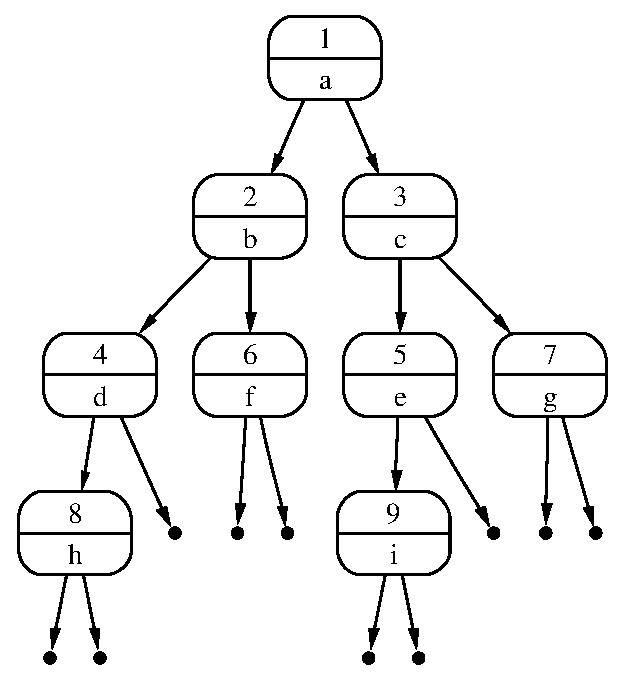
\epsfig{file=heap-with-holes,scale=0.7}} 
  \caption{Ein Heap}
  \label{fig:heap-list}
\end{figure}


Da Heaps bin�re
B�ume sind, k�nnen wir Sie ganz �hnlich wie geordnete bin�re B�ume  implementieren. 
Wir stellen zun�chst Gleichungen auf, die die Implementierung der verschiedenen Methoden
beschreiben.  Wir beginnen mit der  Methode \textsl{top}.  Es gilt:
\begin{enumerate}
\item $\textsl{nil}.\textsl{top}() = \Omega$.
\item $\textsl{node}(k,v,l,r).\textsl{top}() = \pair(k,v)$,

      denn aufgrund der Heap-Bedingung wird der Wert mit der h�chsten Priorit�t 
      an der Wurzel gespeichert.
\end{enumerate}
Die Methoden \textsl{insert} m�ssen wir nun so implementieren, dass
sowohl die Balancierungs-Bedingung als auch die Heap-Bedingung erhalten bleiben.
\begin{enumerate}
\item $\textsl{nil}.\textsl{insert}(k,v) = \textsl{node}(k,v,\textsl{nil}, \textsl{nil})$.
\item $k_{\mathrm{top}} \leq k \;\wedge\; l.\textsl{count}() \leq r.\textsl{count}() \;\rightarrow $   \\[0.1cm]
      \hspace*{1.3cm} 
      $\textsl{node}(k_{\mathrm{top}},v_\mathrm{top},l,r).\textsl{insert}(k,v) =
                 \textsl{node}\bigl(k_\mathrm{top},v_\mathrm{top},l.\textsl{insert}(k,v), r\bigr)$.

      Falls das einzuf�gende Paar eine geringere oder dieselbe Priorit�t hat wie das
      Paar, welches sich an der Wurzel befindet, und falls zus�tzlich die Zahl der Paare im linken Teilbaum
      kleiner-gleich der Zahl der Paare im rechten Teilbaum ist, dann f�gen wir das
      Paar im linken Teilbaum ein.
\item $k_{\mathrm{top}} \leq k \;\wedge\; l.\textsl{count}() > r.\textsl{count}() \;\rightarrow $   \\[0.1cm]
      \hspace*{1.3cm} 
      $\textsl{node}(k_{\mathrm{top}},v_\mathrm{top},l,r).\textsl{insert}(k,v) =
                 \textsl{node}\bigl(k_\mathrm{top},v_\mathrm{top},l,r.\textsl{insert}(k,v)\bigr)$.

      Falls das einzuf�gende Paar eine geringere oder dieselbe Priorit�t hat als das
      Paar an der Wurzel und falls zus�tzlich die Zahl der Paare im linken Teilbaum
      gr��er als die Zahl der Paare im rechten Teilbaum ist, dann f�gen wir das
      Paar im rechten Teilbaum ein.
\item $k_{\mathrm{top}} > k \;\wedge\; l.\textsl{count}() \leq r.\textsl{count}() \;\rightarrow $ \\[0.1cm]
      \hspace*{1.3cm} 
      $\textsl{node}(k_{\mathrm{top}},v_\mathrm{top},l,r).\textsl{insert}(k,v) =
                 \textsl{node}\bigl(k,v,l.\textsl{insert}(k_\mathrm{top},v_\mathrm{top}), r\bigr)$.

      Falls das einzuf�gende Paar eine h�here Priorit�t hat als das Paar an
      der Wurzel, dann m�ssen wir das neu einzuf�gende Paar an der Wurzel
      positionieren.  Das Paar, das dort vorher steht, f�gen wir in den linken
      Teilbaum ein, falls  die Zahl der Paare im linken Teilbaum
      kleiner-gleich der Zahl der Paare im rechten Teilbaum ist.
\item $k_{\mathrm{top}} > k \;\wedge\; l.\textsl{count}() > r.\textsl{count}() \;\rightarrow $ \\[0.1cm] 
      \hspace*{1.3cm} 
      $\textsl{node}(k_{\mathrm{top}},v_\mathrm{top},l,r).\textsl{insert}(k,v) =
                 \textsl{node}\bigl(k,v,l,r.\textsl{insert}(k_\mathrm{top},v_\mathrm{top})\bigr)$.

      Falls wir das einzuf�gende Paar an der Wurzel
      positionieren m�ssen und die Zahl der Paare im linken Teilbaum
      gr��er als die Zahl der Paare im rechten Teilbaum ist,
      dann m�ssen wir das Paar, das vorher an der Wurzel stand, im rechten Teilbaum
      einf�gen.
\end{enumerate}
Als n�chstes beschreiben wir die Implementierung der Methode \textsl{remove}.
\begin{enumerate}
\item $\textsl{nil}.\textsl{remove}() = \textsl{nil}$,

      denn aus dem leeren Heap ist nichts mehr zu entfernen.
\item $\textsl{node}(k,v,\textsl{nil},r).\textsl{remove}() = r$,
  
\item $\textsl{node}(k,v,l,\textsl{nil}).\textsl{remove}() = l$,

      denn wir entfernen immer das Paar mit der h�chsten Priorit�t und das ist an der
      Wurzel.  Wenn einer der beiden Teilb�ume leer ist, k�nnen wir einfach den anderen
      zur�ck geben.

      Jetzt betrachten wir die F�lle, wo keiner der beiden Teilb�ume leer ist.
      Dann muss entweder das Paar an der Wurzel des linken Teilbaums
      oder das Paar an der Wurzel des rechten Teilbaums an die Wurzel aufr�cken.
      Welches dieser beiden Paare wir nehmen, h�ngt davon ab, welches dr Paare die h�here
      Priorit�t hat.
\item $k_1 \leq k_2 \;\wedge\; l = \textsl{node}(k_1,v_1,l_1,r_1) \;\wedge\; r =
      \textsl{node}(k_2,v_2,l_2,r_2) \;\rightarrow$ \\[0.1cm] 
      \hspace*{1.3cm} 
      $\textsl{node}(k,v,l,r).\textsl{remove}() =      \textsl{node}(k_1,v_1,l.\textsl{remove}(),r)$,

      denn wenn das Paar an der Wurzel des linken Teilbaums eine h�here Priorit�t hat
      als das Paar an der Wurzel des rechten Teilbaums, dann r�ckt dieses Paar an
      die Wurzel auf und muss folglich aus dem linken Teilbaum gel�scht werden.
\item $k_1 > k_2 \;\wedge\; l = \textsl{node}(k_1,v_1,l_1,r_1) \;\wedge\; r = \textsl{node}(k_2,v_2,l_2,r_2) \rightarrow$ \\[0.1cm]
      \hspace*{1.3cm} 
      $\textsl{node}(k,v,l,r).\textsl{remove}() = \textsl{node}(k_2,v_2,l,r.\textsl{remove}())$,

      denn wenn das Paar an der Wurzel des rechten Teilbaums eine h�here Priorit�t hat
      als das Paar an der Wurzel des linken Teilbaums, dann r�ckt dieses Paar an
      die Wurzel auf und muss folglich aus dem rechten Teilbaum gel�scht werden.  
\end{enumerate}
An dieser Stelle wird der aufmerksame Leser vermutlich bemerken, dass die obige
Implementierung der Methode \textsl{remove} die Balancierungs-Bedingung verletzt.
Es ist nicht schwierig, die Implementierung so abzu�ndern, dass die
Balancierungs-Bedingung erhalten bleibt. Es zeigt sich jedoch, dass die
Balancierungs-Bedingung  nur beim Aufbau eines Heaps mittels \textsl{insert}() wichtig ist,
denn dort garantiert sie, dass die H�he des Baums in logarithmischer Weise von der Zahl
seiner Knoten abh�ngt.  Beim L�schen wird die H�he des Baums sowieso nur kleiner, also
brauchen wir uns da keine Sorgen machen.

\section{Implementierung in \textsl{Java}}

\begin{figure}[!h]
  \centering
\begin{Verbatim}[ frame         = lines, 
                  framesep      = 0.3cm, 
                  labelposition = bottomline,
                  numbers       = left,
                  numbersep     = -0.2cm,
                  xleftmargin   = 0.0cm,
                  xrightmargin  = 0.0cm
                ]
    public abstract class HeapNode<Key extends Comparable<Key>, Value>
    {
        protected int mCount;
    
        public abstract Pair<Key, Value> top();
        public abstract BinaryHeapNode<Key, Value> insert(Key key, Value value);
        public abstract HeapNode<Key, Value> remove();    
        public abstract boolean isEmpty();
    }
\end{Verbatim}
\vspace*{-0.3cm}
  \caption{Die abstrakte Klasse \textsl{HeapNode}.}
  \label{fig:HeapNode}
\end{figure}
Zun�chst implementieren wir eine abstrakte Klasse \textsl{HeapNode}.  Elemente dieser
Klasse sollen Heaps repr�sentieren und zwar sowohl leere Heaps als auch nicht-leere Heaps.
Abbildung \ref{fig:HeapNode} auf Seite \pageref{fig:HeapNode} zeigt die Implementierung.
Wir haben eine Member-Variable mit dem Namen \texttt{mCount} in Zeile 3 definiert.
Diese Variable gibt die Zahl der in dem Heap abgespeicherten Werte an.

Wir werden uns mit der Implementierung der Methode $\textsl{change}()$ erst sp�ter
besch�ftigen. Daher fehlt diese Methode in der Klasse \textsl{HeapNode}.
Statt dessen haben wir eine zus�tzliche Methode \textsl{isEmpty}(), die wir sp�ter bei der
Implementierung der Methoden \textsl{insert}() und \textsl{remove}() benutzen werden.

\begin{figure}[!h]
  \centering
\begin{Verbatim}[ frame         = lines, 
                  framesep      = 0.3cm, 
                  labelposition = bottomline,
                  numbers       = left,
                  numbersep     = -0.2cm,
                  xleftmargin   = 0.0cm,
                  xrightmargin  = 0.0cm
                ]
    public class EmptyHeapNode<Key extends Comparable<Key>, Value> 
        extends HeapNode<Key, Value>
    {
        public EmptyHeapNode() {
            mCount = 0;
        }    
        public Pair<Key, Value> top() {
            return null;
        }
        public BinaryHeapNode<Key, Value> insert(Key key, Value value) {
            return new BinaryHeapNode<Key, Value>(key, value);
        }        
        public HeapNode<Key, Value> remove() {
            return this;
        }
        public boolean isEmpty() {
            return true;
        }
    }
\end{Verbatim}
\vspace*{-0.3cm}
  \caption{Die Klasse \textsl{EmptyHeapNode}.}
  \label{fig:EmptyHeapNode}
\end{figure}

Abbildung \ref{fig:EmptyHeapNode} auf Seite \pageref{fig:EmptyHeapNode} zeigt die
Implementierung der Klasse \textsl{EmptyHeapNode}.  Elemente dieser Klasse repr�sentieren
den leeren Heap \textsl{nil}.  Im Konstruktor setzen wir in Zeile 5 die Member-Variable
\texttt{mCount} auf 0, denn der leere Heap enth�lt keine Werte. Die Methode \textsl{top}()
gibt \texttt{null} zur�ck, denn es gibt ja keinen sinnvollen Wert, den wir hier zur�ck
geben k�nnen.   Die Methode \textsl{insert}() erzeugt einen neuen Knoten vom Typ
\textsl{BinaryHeapNode}, der dann zur�ck gegeben wird. 


\begin{figure}[!h]
  \centering
\begin{Verbatim}[ frame         = lines, 
                  framesep      = 0.3cm, 
                  labelposition = bottomline,
                  numbers       = left,
                  numbersep     = -0.2cm,
                  xleftmargin   = 0.0cm,
                  xrightmargin  = 0.0cm
                ]
    public class BinaryHeapNode<Key extends Comparable<Key>, Value> 
        extends HeapNode<Key, Value>
    {
        private Key                  mKey;    // The priority associated with the value.
        private Value                mValue;  // The value.
        private HeapNode<Key, Value> mLeft;   // The root of the left subtree.
        private HeapNode<Key, Value> mRight;  // The root of the right subtree.
    
        public BinaryHeapNode(Key key, Value value) {
            mKey    = key;
            mValue  = value;
            mLeft   = new EmptyHeapNode<Key, Value>();
            mRight  = new EmptyHeapNode<Key, Value>();
            mCount  = 1;
        }    
        public Pair<Key, Value> top() {
            return new Pair<Key, Value>(mKey, mValue);
        }
        public BinaryHeapNode<Key, Value> insert(Key key, Value value)
        {
            ++mCount;
            int cmp = key.compareTo(mKey);
            if (cmp < 0) {                         
                if (mLeft.mCount > mRight.mCount) {
                    mRight = mRight.insert(mKey, mValue);
                } else {
                    mLeft = mLeft.insert(mKey, mValue);
                }
                mKey   = key;
                mValue = value;
            } else {
                if (mLeft.mCount > mRight.mCount) {
                    mRight = mRight.insert(key, value);
                } else {
                    mLeft = mLeft.insert(key, value);
                }
            }
            return this;
        }        
        public boolean isEmpty() {
            return false;
        }
\end{Verbatim}
\vspace*{-0.3cm}
  \caption{Die Klasse \textsl{BinaryHeapNode}, Teil I.}
  \label{fig:BinaryHeapNode-I}
\end{figure}
Die Klasse \textsl{BinaryHeapNode}, deren Implementierung in den Abbildungen
\ref{fig:BinaryHeapNode-I} und \ref{fig:BinaryHeapNode-II} auf den Seiten
\pageref{fig:BinaryHeapNode-I} und \pageref{fig:BinaryHeapNode-II} gezeigt wird,
repr�sentiert einen Knoten der Form \\[0.1cm]
\hspace*{1.3cm} 
$\textsl{node}(\texttt{mKey}, \mathtt{mValue}, \mathtt{mLeft}, \mathtt{mRight})$. 
\\[0.1cm]
Die Implementierung setzt die rekursiven Gleichungen, die wir im vorhergehenden
Unterabschnitt gezeigt haben, 1-zu-1 um.  Diskutiert werden muss h�chstens noch die
Implementierung der Methode \textsl{remove}.  Wenn der Kontrollfluss in Zeile 51 ankommt,
dann ist klar, dass weder der linke Teilbaum \texttt{mLeft} noch der rechte Teilbaum
\texttt{mRight} leer ist.
Daher sind diese Teilb�ume Objekte der Klasse \textsl{BinaryHeapNode} und wir k�nnen
\texttt{mLeft} und \texttt{mRight} auf den Typ \textsl{BinaryHeapNode} casten.
Dies ist notwendig, weil wir auf die Schl�ssel, die an der Wurzel dieser B�ume
abgespeichert sind, zur�ckgreifen m�ssen.  Das geht aber nur, wenn diese den Typ
\textsl{BinaryHeapNode} haben, denn nur in diesem Typ sind die Member-Variablen
\texttt{mKey} und \texttt{mValue} definiert.

\begin{figure}[!h]
  \centering
\begin{Verbatim}[ frame         = lines, 
                  framesep      = 0.3cm, 
                  firstnumber   = last,
                  labelposition = bottomline,
                  numbers       = left,
                  numbersep     = -0.2cm,
                  xleftmargin   = 0.0cm,
                  xrightmargin  = 0.0cm
                ]
        public HeapNode<Key, Value> remove() {
            --mCount;
            if (mLeft.isEmpty()) {
                return mRight;
            } 
            if (mRight.isEmpty()) {
                return mLeft;
            }
            BinaryHeapNode<Key, Value> left  = (BinaryHeapNode<Key, Value>) mLeft;
            BinaryHeapNode<Key, Value> right = (BinaryHeapNode<Key, Value>) mRight;
            Key leftKey  = left .mKey;
            Key rightKey = right.mKey;
            if (leftKey.compareTo(rightKey) < 0) {
                mKey   = left.mKey;
                mValue = left.mValue;
                mLeft  = mLeft.remove();
            } else {
                mKey   = right.mKey;
                mValue = right.mValue;
                mRight = mRight.remove();
            }
            return this;
        }
    }
\end{Verbatim}
\vspace*{-0.3cm}
  \caption{Die Klasse \textsl{BinaryHeapNode}, Teil II.}
  \label{fig:BinaryHeapNode-II}
\end{figure}

\subsection{Implementierung der Methode \textsl{change}}
Als letztes beschreiben wir, wie die Methode \textsl{change}() effizient implementiert werden kann.
Wir setzen voraus, dass bei einem Aufruf der Form \\[0.1cm]
\hspace*{1.3cm} $h.\textsl{change}(k,v)$ \\[0.1cm]
die Priorit�t des Elements $v$ verg��ert wird.  Ist $p = \textsl{node}(k',v,l,r)$ der Knoten,
in dem der Wert $v$ gespeichert ist, dann gilt also $k < k'$.  Um die Priorit�t von $v$
abzu�ndern, m�ssen wir zun�chst den Knoten $p$ finden.  Eine M�glichkeit um diesen Knoten
zu finden besteht darin, dass wir einfach alle Knoten des Heaps durchsuchen und den dort
gespeicherten Wert mit $v$ vergleichen.  Wenn der Heap aus  $n$ Knoten besteht,
dann brauchen wir dazu insgesamt $n$ Vergleiche.  Damit w�rde die Implementierung der Methode
\textsl{change}() eine Komplexit�t $\Oh(n)$ haben.  Es geht aber schneller.  Die Idee ist,
dass wir in einer Hash-Tabelle\footnote{Wir k�nnen an dieser Stelle auch eine
  \textsl{AVL}-Baum nehmen um die Zuordnung der Knoten zu den Werten zu speichern.
Damit dies m�glich ist, muss allerdings auf der Menge der Werte eine totale Ordnung existieren.
}
 die Zuordnung der Knoten zu den Werten speichern.  
Damit eine eindeutige Zuordnung von Werten zu Knoten �berhaupt m�glich ist, gehen wir
davon aus, dass jeder Wert h�chstens einmal in einem Heap auftritt.
Die HashTabelle realisiert dann die Funktion \\[0.1cm]
\hspace*{1.3cm} $\textsl{nodeMap}: \textsl{Value} \rightarrow \textsl{Node}$, \\[0.1cm]
f�r welche die Invariante \\[0.1cm]
\hspace*{1.3cm} $\textsl{nodeMap}(v_1) = \textsl{node}(k,v_2,l,r) \rightarrow v_1 = v_2$ \\[0.1cm]
gilt. Mit andern Worten: Der Aufruf $\textsl{nodeMap}(v)$ gibt den Knoten zur�ck, in dem
der Wert $v$ gespeichert ist.  

Wenn wir nun den Knoten $p = \textsl{node}(k',v,l,r)$ gefunden haben, in dem der Wert $v$
gespeichert ist, dann reicht es nicht aus, wenn wir in dem Knoten $p$ einfach die Priorit�t $k'$
durch $k$ ersetzen, denn es k�nnte sein, dass dann die Heap-Bedingung verletzt wird und
der Schl�ssel, der in dem Knoten $p$ gespeichert ist, eine h�here Priorit�t hat als der
Vater-Knoten dieses Knotens.  In diesem Fall m�ssen wir das Paar, dass in diesem Knoten
gespeichert ist, mit dem Paar, das in dem Vater-Knoten gespeichert ist, vertauschen.
Anschlie�end k�nnte es sein, dass f�r den Vater-Knoten und dessen Vater-Knoten die
Heap-Bedingung verletzt ist, so dass wir nun rekursiv den Vater-Knoten weiter untersuchen
m�ssen.  Das Verfahren l�sst sich nicht ohne weiteres durch rekursive Gleichungen
beschreiben, denn wenn wir einen bin�ren Knoten in der Form
\[ \textsl{node}(k,v,l,r) \]
darstellen, haben wir keine Informationen �ber den Vaterknoten.  Wir f�hren daher zun�chst
ein Paar Hilfsfunktionen ein.
\begin{enumerate}
\item $\textsl{parent}: \textsl{Node} \rightarrow \textsl{Node} \cup \{ \Omega \}$

      F�r jeden Knoten $n$ gibt der Aufruf $n.\textsl{parent}(n)$ den Vaterknoten zur�ck.
      Falls zu dem Knoten $n$ kein Vaterknoten existiert, wird statt dessen $\Omega$
      zur�ck geliefert.
\item $\textsl{nodeMap}: \textsl{Value} \rightarrow \textsl{Node} \cup \{ \Omega \}$

      F�r einen Wert $v$ liefert der Aufruf $\textsl{nodeMap}(v)$ den Knoten, in dem der Wert
      $v$ gespeichert ist.
\item $\textsl{key}: \textsl{Node} \rightarrow \textsl{Key}$

      F�r einen Knoten $n$ liefert der Aufruf $n.\textsl{key}()$ den in dem Knoten
      gespeicherten Schl�ssel zur�ck.

\item $\textsl{value}: \textsl{Node} \rightarrow \textsl{Value}$

      F�r einen Knoten $n$ liefert der Aufruf $n.\textsl{value}()$ den in dem Knoten
      gespeicherten Wert zur�ck.
\end{enumerate}
Damit k�nnen wir nun eine Methode $\textsl{upheap}()$ entwickeln, so dass der Aufruf
$n.\textsl{upheap}()$ die Heap-Bedingung an dem Knoten $n$ wiederherstellt, falls diese
dadurch verletzt wurde, dass die an dem Knoten gespeicherte Priorit�t erh�ht wurde.
Abbildungen \ref{fig:upheap.pseudo} zeigt den Pseudo-Code, den wir jetzt im Detail diskutieren.

\begin{figure}[!ht]
\centering
\begin{Verbatim}[ frame         = lines, 
                  framesep      = 0.3cm, 
                  labelposition = bottomline,
                  numbers       = left,
                  numbersep     = -0.2cm,
                  xleftmargin   = 0.8cm,
                  xrightmargin  = 0.8cm,
                  commandchars  = \\\{\},
                  codes         = {\catcode`$=3\catcode`_=8\catcode`^=7},
                ]
    n.upheap() \{
        k\(_1\) := n.key();
        v\(_1\) := n.value();
        p  := n.parent();
        if (p = null) \{ 
            return;
        \}
        k\(_2\) := p.key();
        v\(_2\) := p.value();
        if (k\(_1\) < k\(_2\)) \{
            n.key()   := k\(_2\);
            n.value() := v\(_2\);
            p.key()   := k\(_1\);
            p.value() := v\(_1\);
            \textsl{nodeMap}(v\(_2\)) := n;
            \textsl{nodeMap}(v\(_1\)) := p;
            p.upheap();
        \}
    \}
\end{Verbatim}
\vspace*{-0.3cm}
\caption{Pseudo-Code zur Implementierung der Methode \textsl{upheap}()}
\label{fig:upheap.pseudo}
\end{figure}%\$ 

\begin{enumerate}
\item Zun�chst bezeichnen wir die Priorit�t, die an dem Knoten $n$ gespeichert ist,
      mit $k_1$ und den zugeh�rigen Wert mit $v_1$.
\item Der Vaterknoten von $n$ wird mit $p$ bezeichnet und die Priorit�t, die dort gespeichert ist,
      wird mit $k_2$, der zugeh�rige Wert mit $v_2$ bezeichnet.  

      Falls der Knoten $n$
      bereits der Wurzel-Knoten ist, so exitiert kein  Vaterknoten und damit kann die
      Heap-Bedingung auch nicht verletzt sein, so dass die Methode $\textsl{upheap}()$
      beendet werden kann.
\item Hat nun der an dem Knoten $n$ gespeicherte Wert eine h�here Priorit�t als der an dem
      Vaterknoten $p$ gespeicherte Wert, so werden die Werte (inklusive Priorit�ten), die
      an den Knoten $n$ und $p$ gespeichert sind, vertauscht.  

      Zus�tzlich achten wir darauf, dass die in der Tabelle \textsl{nodeMap} hinterlegte
      Zuordung von Werten zu Knoten korrekt bleibt.
\item Schlie�lich m�ssen wir die Methode \textsl{upheap} rekursiv f�r den Vaterknoten aufrufen.
\end{enumerate}


\begin{figure}[!h]
  \centering
\begin{Verbatim}[ frame         = lines, 
                  framesep      = 0.3cm, 
                  labelposition = bottomline,
                  numbers       = left,
                  numbersep     = -0.2cm,
                  xleftmargin   = 0.0cm,
                  xrightmargin  = 0.0cm
                ]
    import java.util.*;
    
    public abstract class HeapNode<Key extends Comparable<Key>, Value>
    {
        protected int                        mCount;  // the number of nodes
        protected BinaryHeapNode<Key, Value> mParent; // parent of this node
        protected Map<Value, BinaryHeapNode<Key, Value>> mNodeMap;
    
        public abstract Pair<Key, Value> top();    
        public abstract BinaryHeapNode<Key, Value> insert(Key key, Value value);
        public abstract HeapNode<Key, Value> remove();
        public abstract void change(Key k, Value v);
        public abstract boolean isEmpty();
    }
\end{Verbatim}
\vspace*{-0.3cm}
  \caption{Die abstrakte Klasse \textsl{HeapNode}.}
  \label{fig:HeapNode-2}
\end{figure}

Die Abbildungen \ref{fig:HeapNode-2},  \ref{fig:EmptyHeapNode-2},
\ref{fig:BinaryHeapNode-2-I},  \ref{fig:BinaryHeapNode-repair-2},
\ref{fig:BinaryHeapNode-repair-2}, \ref{fig:BinaryHeapNode-change} und \ref{fig:HeapTree} 
auf den folgenden Seiten zeigen eine vollst�ndige
Implementierung des abstrakten Daten-Typs \textsl{PrioQueue}.  Wir diskutieren nun die
Ver�nderungen gegen�ber der bisher gezeigten Implementierung.  
Wir beginnen mit der abstrakten Klasse \textsl{HeapNode}, die in Abbildung
\ref{fig:HeapNode-2} auf Seite \pageref{fig:HeapNode-2} gezeigt wird.
Gegen�ber der Implementierung in Abbildung \ref{fig:HeapNode} auf Seite \ref{fig:HeapNode}
gibt es die folgenden �nderungen.
\begin{enumerate}
\item Die Klasse enth�lt eine zus�tzliche Member-Variable \texttt{mParent}, die in Zeile 6
      definiert wird.  Hierbei handelt es sich um eine Referenz auf den Vater-Knoten.
      Diese Referenz ist notwendig f�r die Implementierung der Methode \textsl{change}(),
      denn dort m�ssen wir nach einer �nderung der Priorit�t eines Schl�ssel �berpr�fen, 
      ob die Priorit�t des Vater-Knotens immer noch gr��er ist als die Priorit�t des Knotens dessen
      Priorit�t wir ge�ndert haben.
\item Au�erdem enth�lt jeder Knoten jetzt eine Referenz auf die Abbildung
      \textsl{nodeMap}, in der die Zuordnung der Knoten zu den Werten gespeichert wird.
      Diese Referenz wird in der in Zeile 7 definierten Member-Variable \texttt{mNodeMap}
      gespeichert.
\end{enumerate}

\begin{figure}[!ht]
  \centering
\begin{Verbatim}[ frame         = lines, 
                  framesep      = 0.3cm, 
                  labelposition = bottomline,
                  numbers       = left,
                  numbersep     = -0.2cm,
                  xleftmargin   = 0.0cm,
                  xrightmargin  = 0.0cm
                ]
    import java.util.*;
    
    public class EmptyHeapNode<Key extends Comparable<Key>, Value> 
        extends HeapNode<Key, Value>
    {
        public EmptyHeapNode(BinaryHeapNode<Key, Value>             parent,
                             Map<Value, BinaryHeapNode<Key, Value>> nodeMap) 
        {
            mParent  = parent;
            mNodeMap = nodeMap;
            mCount   = 0;
        }    
        public Pair<Key, Value> top() {
            return null;
        }
        public BinaryHeapNode<Key, Value> insert(Key key, Value value) {
            BinaryHeapNode<Key, Value> binaryNode =
                new BinaryHeapNode<Key, Value>(key, value, mParent, mNodeMap);
            mNodeMap.put(value, binaryNode);
            return binaryNode;
        }        
        public HeapNode<Key, Value> remove()        { return this; }
        public void    change(Key key, Value value) {}
        public boolean isEmpty()                    { return true; }
    }
\end{Verbatim}
\vspace*{-0.3cm}
  \caption{Die Klasse  \textsl{EmptyHeapNode}.}
  \label{fig:EmptyHeapNode-2}
\end{figure}

Als n�chstes diskutieren wir die �nderungen in der Klasse \textsl{EmptyHeapNode}.
\begin{enumerate}
\item Da die Klasse nun zwei zus�tzliche Member-Variablen von der Klasse \textsl{HeapNode}
      erbt, hat der Konstruktor, der in Zeile 6 -- 12 implementiert ist, zwei zus�tzliche
      Argumente, die zur Initialisierung der beiden Member-Variablen \texttt{mParent}
      und \texttt{mNodeMap} genutzt werden.
\item Die Implementierung der Methode \textsl{insert}() ist nun aufwendiger, denn wir
      m�ssen den erzeugten Knoten in die HashTabelle \texttt{mNodeMap} eintragen.
\item Die Implementierung der Methode \textsl{change}(), die ebenfalls neu hinzu gekommen
      ist, ist f�r einen leeren Knoten trivial. 
\end{enumerate}

\begin{figure}[!ht]
  \centering
\begin{Verbatim}[ frame         = lines, 
                  framesep      = 0.3cm, 
                  labelposition = bottomline,
                  numbers       = left,
                  numbersep     = -0.2cm,
                  xleftmargin   = 0.0cm,
                  xrightmargin  = 0.0cm
                ]
    import java.util.*;
    
    public class BinaryHeapNode<Key extends Comparable<Key>, Value> 
        extends HeapNode<Key, Value>
    {
        private Key                  mKey;
        private Value                mValue;
        private HeapNode<Key, Value> mLeft;
        private HeapNode<Key, Value> mRight;
    
        public BinaryHeapNode(Key                                    key, 
                              Value                                  value, 
                              BinaryHeapNode<Key, Value>             parent,
                              Map<Value, BinaryHeapNode<Key, Value>> nodeMap)
        {
            mKey     = key;
            mValue   = value;
            mParent  = parent;
            mNodeMap = nodeMap;
            mLeft    = new EmptyHeapNode<Key, Value>(this, nodeMap);
            mRight   = new EmptyHeapNode<Key, Value>(this, nodeMap);
            mCount   = 1;
        }
        public Pair<Key, Value> top() {
            return new Pair<Key, Value>(mKey, mValue);
        }
        public BinaryHeapNode<Key, Value> insert(Key key, Value value) {
            ++mCount;
            int cmp = key.compareTo(mKey);
            if (cmp < 0) {
                mNodeMap.remove(mValue);
                if (mLeft.mCount > mRight.mCount) {
                    mRight = mRight.insert(mKey, mValue);
                } else {
                    mLeft  = mLeft .insert(mKey, mValue);
                }
                mKey   = key;
                mValue = value;
                mNodeMap.put(value, this);
            } else {
                if (mLeft.mCount > mRight.mCount) {
                    mRight = mRight.insert(key, value);
                } else {
                    mLeft  = mLeft .insert(key, value);
                }
            }
            return this;
        }
\end{Verbatim}
\vspace*{-0.3cm}
  \caption{Die Klasse  \textsl{BinaryHeapNode}, 1. Teil.}
  \label{fig:BinaryHeapNode-2-I}
\end{figure}

\begin{figure}[!ht]
  \centering
\begin{Verbatim}[ frame         = lines, 
                  framesep      = 0.3cm, 
                  firstnumber   = last,
                  labelposition = bottomline,
                  numbers       = left,
                  numbersep     = -0.2cm,
                  xleftmargin   = 0.0cm,
                  xrightmargin  = 0.0cm
                ]
        public HeapNode<Key, Value> remove() {
            mNodeMap.remove(mValue);
            if (mLeft.isEmpty()) {
                mRight.mParent = mParent;
                return mRight;
            } 
            if (mRight.isEmpty()) {
                mLeft.mParent = mParent;
                return mLeft;
            }
            --mCount;
            BinaryHeapNode<Key, Value> left  = (BinaryHeapNode<Key, Value>) mLeft;
            BinaryHeapNode<Key, Value> right = (BinaryHeapNode<Key, Value>) mRight;
            Key leftKey  = left .mKey;
            Key rightKey = right.mKey;
            if (leftKey.compareTo(rightKey) < 0) {
                mKey   = left.mKey;
                mValue = left.mValue;
                mLeft  = mLeft.remove();
            } else {
                mKey   = right.mKey;
                mValue = right.mValue;
                mRight = mRight.remove();
            }
            mNodeMap.put(mValue, this);
            repair();
            return this;
        }
        private void repair() {
            if (Math.abs(mLeft.mCount - mRight.mCount) <= 1) {
                return;
            }
            if (mLeft.mCount == mRight.mCount + 2) {
                BinaryHeapNode<Key, Value> left  = (BinaryHeapNode<Key, Value>) mLeft;
                Key   key   = left.mKey;
                Value value = left.mValue;
                mLeft  = mLeft.remove();
                mRight = mRight.insert(key, value);
                return;
            } else if (mRight.mCount == mLeft.mCount + 2) {
                BinaryHeapNode<Key, Value> right = (BinaryHeapNode<Key, Value>) mRight;
                Key   key   = right.mKey;
                Value value = right.mValue;
                mRight = mRight.remove();
                mLeft  = mLeft .insert(key, value);
                return;
            }
        }       
\end{Verbatim}
\vspace*{-0.3cm}
  \caption{Die Methoden  \textsl{remove} und \textsl{repair}.}
  \label{fig:BinaryHeapNode-repair-2}
\end{figure}

\begin{figure}[!ht]
  \centering
\begin{Verbatim}[ frame         = lines, 
                  framesep      = 0.3cm, 
                  firstnumber   = last,
                  labelposition = bottomline,
                  numbers       = left,
                  numbersep     = -0.2cm,
                  xleftmargin   = 0.0cm,
                  xrightmargin  = 0.0cm
                ]
        public void change(Key key, Value value) {
            BinaryHeapNode<Key, Value> node = mNodeMap.get(value);
            node.mKey = key;
            node.upHeap();
        }
        private void upHeap() 
        {
            if (mParent == null) {
                return;  // heap condition trivially satisfied
            }
            Key   parentKey   = mParent.mKey;
            Value parentValue = mParent.mValue;
            if (parentKey.compareTo(mKey) <= 0) {
                return;  // heap condition already satisfied
            }
            mNodeMap.put(mValue, mParent);
            mNodeMap.put(parentValue, this);
            mParent.mKey   = mKey;
            mParent.mValue = mValue;
            mKey           = parentKey;
            mValue         = parentValue;
            mParent.upHeap();
        }    
        public boolean isEmpty() {
            return false;
        }
    }
\end{Verbatim}
\vspace*{-0.3cm}
  \caption{Die Methoden \textsl{change} und \textsl{upheap}.}
  \label{fig:BinaryHeapNode-change}
\end{figure}

In der Klasse \textsl{BinaryHeapNode} gibt es die meisten �nderungen.
\begin{enumerate}
\item Zun�chst bekommt der Konstruktor zwei zus�tzliche Argumente um die 
      Member-Variablen \texttt{mParent} und \texttt{mNodeMap} zu initialisieren. 
\item Bei der Methode \textsl{insert}() behandeln wir in den Zeilen 31 -- 39 
      den Fall, dass der neu einzuf�gende Wert eine h�here Priorit�t hat als der Wert, der
      momentan an der Wurzel steht.  Daher wird der neu einzuf�gende Wert
      jetzt an der Wurzel gespeichert und der Wert, der vorher dort stand,
      wird entweder in den linken Teilbaum \texttt{mLeft} oder in den
      rechten Teilbaum \texttt{mRight} eingef�gt.

      Wir m�ssen hier darauf achten, dass die HashTabelle \texttt{mNodeMap} konsistent
      bleibt.  Daher entfernen wir in Zeile 31 die Zuordnung von \texttt{mValue} zu dem
      Knoten \texttt{this} aus der Tabelle und f�gen in Zeile 39 statt dessen 
      die Zuordnung von dem neu eingef�gten Wert \textsl{value} zu dem Knoten
      \texttt{this} ein.
\item Entsprechende �nderungen gibt es auch in der Methode \texttt{remove}.
      Wir l�schen zun�chst in Zeile 51 die unter dem Schl�ssel \texttt{mValue}
      abgespeicherte Zuordnung, denn diesen Wert wollen wir ja entfernen.
      Da wir anschlie�end entweder den Wert aus dem linken oder dem rechten Teilbaum 
      nach oben ziehen, m�ssen wir f�r den Wert, den wir nach oben gezogen haben,
      eine Zuordnung in der HashTabelle \texttt{mNodeMap} eintragen. Dies geschieht
      in Zeile 73.

      In der Methode \texttt{remove} gibt es in den Zeile 52 und 56 noch eine wichtige 
      �nderung: Da wir dort den Knoten im rechten bzw.~linken Teilbaum nach oben schieben,
      m�ssen wir dessen Zeiger zum Vaterknoten umsetzen, denn sonst w�rde dieser immer noch
      auf einen Knoten zeigen, den wir l�schen.
\item Zus�tzlich sehen Sie in den Zeilen 77 bis 98 noch die Methode $\textsl{repair}()$,
      mit der die Balan\-cierungs-Bedingung an einem Knoten dann wiederhergestellt werden kann, 
      falls sie durch einen vorhergehenden Aufruf von $\textsl{remove}()$ verletzt worden ist.
      Die Idee, die dieser Methode zu Grunde liegt, ist simpel:  Falls ein Teilbaum einen Knoten
      mehr als erlaubt enth�lt, so wird in diesem Teilbaum ein Knoten entfernt und dann in den
      andern Teilbaum eingef�gt.
\item Bei der Implementierung der Methode \textsl{change}() suchen wir zun�chst
      den Knoten, an dem der zu �ndernde Wert gespeichert ist.  Anschlie�end
      �ndern wir die in diesem Knoten abgespeicherte Priorit�t.  Dabei kann die
      Heap-Bedingung verletzt werden: Es k�nnte sein, dass der Knoten jetzt eine h�here
      Priorit�t hat als der Vater dieses Knotens.  Um die Heap-Bedingung
      wiederherzustellen rufen wir daher die Methode \texttt{upHeap}() auf.
\item Die Methode \texttt{upHeap}() pr�ft zun�chst, ob �berhaupt ein Vater-Knoten
      vorhanden ist, denn nur dann kann die Heap-Bedingung verletzt sein.
      Falls ein Vater-Knoten vorhanden ist, wird als n�chstes gepr�ft, ob die 
      Heap-Bedingung verletzt ist.  Wenn dies so ist,
      dann vertauscht die Methode die Priorit�t und den Wert, der im Vater-Knoten
      abgespeichert ist mit der Priorit�t und dem Wert, der in diesem Knoten 
      abgespeichert ist.  Gleichzeitig wird darauf geachtet, dass die HashTabelle
      \texttt{mNodeMap} konsistent bleibt.
      
      Wenn der Wert und die Priorit�t des aktuellen Knotens an den Vater-Knoten
      geschoben  worden sind, dann kann es passieren, dass nun dort die Heap-Bedingung
      verletzt ist.  Daher wird jetzt f�r den Vater-Knoten rekursiv die Methode
      \textsl{upHeap}() aufgerufen.
\end{enumerate}


\begin{figure}[!ht]
  \centering
\begin{Verbatim}[ frame         = lines, 
                  framesep      = 0.3cm, 
                  labelposition = bottomline,
                  numbers       = left,
                  numbersep     = -0.2cm,
                  xleftmargin   = 0.0cm,
                  xrightmargin  = 0.0cm
                ]
    import java.util.*;
    
    public class HeapTree<Key extends Comparable<Key>, Value>
    {
        HeapNode<Key, Value> mRoot;  // this is the node at the root of the tree 
    
        public HeapTree() {
            Map<Value, BinaryHeapNode<Key, Value>> nodeMap = 
                new HashMap<Value, BinaryHeapNode<Key, Value>>();
            mRoot = new EmptyHeapNode<Key, Value>(null, nodeMap);
        }
        public Pair<Key, Value> top() {
            return mRoot.top();
        }    
        public void insert(Key key, Value value) {
            mRoot = mRoot.insert(key, value);
        }
        public void change(Key key, Value value) {
            mRoot.change(key, value);
        }
        public void remove() {
            mRoot = mRoot.remove();
        }    
    }
\end{Verbatim}
\vspace*{-0.3cm}
  \caption{Die Klasse \textsl{HeapTree}.}
  \label{fig:HeapTree}
\end{figure}

Wir betrachten als letztes die
Klasse \textsl{HeapTree}, die in Abbildungen \ref{fig:HeapTree} auf Seite
\pageref{fig:HeapTree} gezeigt wird.  Diese Klasse repr�sentiert einen vollst�ndigen
\textsl{Heap}.  
\begin{enumerate}
\item Der Wurzel-Knoten  des Heaps wird in der Member-Variablen \texttt{mRoot}
      gepeichert. 
\item Au�erdem verwaltet diese Klasse die HashTabelle \textsl{nodeMap}, die
      die Zuordnung zwischen den Werten und den Knoten herstellt.  Diese Tabelle
      wird in dem Konstruktor in Zeile 8 zun�chst als leere Tabelle angelegt.
      Anschlie�end wird ein leerer Knoten erzeugt, der eine Referenz auf die
      gerade angelegte Tabelle erh�lt.  Dieser leere Knoten ist der Wurzel-Knoten
      des Heaps.
\item Die Signaturen der Methoden \textsl{insert}(), \textsl{change}() und
      \textsl{remove}() sind gegen�ber den entsprechenden Methoden in der Klasse
      \textsl{HeapNode} und in den davon abgeleiteten Klassen
      \textsl{EmptyHeapNode} und \textsl{BinaryHeapNode} dahingehend ver�ndert,
      dass diese Methoden nun nichts mehr zur�ck geben. Statt dessen �ndern
      diese Methoden jetzt den zugrunde liegenden Heap \textsl{mRoot}.  Diese
      �nderung der Signaturen ist der Grund f�r die Existenz der Klasse
      \textsl{HeapTree}: In der Klasse \textsl{HeapTree} haben die Methoden
      \textsl{insert}(), \textsl{change}() und \textsl{remove} die Signaturen,
      die wir brauchen und die Methoden �ndern den zugrunde liegenden Heap.  
      In der Klasse \textsl{HeapNode} sind diese Signaturen so nicht m�glich,
      denn beispsielsweise ist es unm�glich, beim Einf�gen aus einem
      \textsl{EmptyHeapNode} einen \textsl{BinaryHeapNode} zu machen, da sich in
      \textsl{Java} der Typ eines Objektes zur Laufzeit nicht �ndern kann.
\end{enumerate}

\subsection{Priorit�ts-Warteschlangen in \textsl{Java}}
In \textsl{Java} werden Priorit�ts-Warteschlangen durch die Klasse \texttt{PriorityQueue<E>}
implementiert.  Als Datenstruktur wird dabei ein Feld verwendet um den zu Grunde liegenden
bin�ren Baum darzustellen.  Bezeichnen wir das Feld mit \texttt{mArray}, so gilt:
\begin{enumerate}
\item Die Wurzel des bin�ren Baums wird in dem Element \texttt{mArray[0]} gespeichert.
\item Wird der Knoten $\textsl{node}(k,v,l,r)$ als \texttt{mArray[i]} abgespeichert,
      so wird der Knoten an der Wurzel des linkes Teilbaum $l$ an der Position $2\cdot i
      +1$ abgespeichert und der Knoten an der Wurzel
      rechte Teilbaum $r$ wird an der Position $2 \cdot (i+1)$ abgespeichert.
\item Wird der Knoten $n$ an der Position $i$ abgespeichert, so findet sich der
      Vater-Knoten von $n$ an der Position $(i - 1) / 2$.
\end{enumerate}
Damit eine solche Feld-basierte Darstellung m�glich ist, ist es erforderlich, die
Balancierungs-Bedingung f�r Heaps etwas abzu�ndern.  Wir skizzieren kurz die Idee,
die der abge�nderten Definition zu Grunde liegt.
\begin{enumerate}
\item Ein bin�rer Baum hei�t \emph{vollst�ndig}, wenn alle Bl�tter des Baums
      den selben Abstand zur Wurzel haben.  Bezeichnen wir die Menge der vollst�ndigen bin�ren
      B�ume mit $\overline{\Bin}$, so k�nnen k�nnen wir die folgende induktive Definition geben:
      \begin{enumerate}
      \item $\textsl{nil} \in \overline{\Bin}$,
      \item $\textsl{node}(k,v,l,r) \in \overline{\Bin} 
             \;\stackrel{\mbox{\scriptsize def}}{\longleftrightarrow}\;
             l \in \overline{\Bin} \,\wedge\, r \in \overline{\Bin} \,\wedge\,
             l.\textsl{height}() = r.\textsl{height}()$ 
      \end{enumerate}
      Abbildung \ref{fig:complete-tree.eps} zeigt einen vollst�ndigen Baum der Tiefe 4.
      Teilen wir die Knoten nach ihrem Abstand $h$ von der Wurzel in verschiedene
      Schichten ein, so sehen wir, dass es auf der Schicht, die von der Wurzel den Abstand
      $h$ hat, insgesamt $2^h$ Knoten gibt.

      \begin{figure}[!ht]
        \centering
        \epsfig{file=Abbildungen/complete-tree.eps}
        \caption{Ein vollst�ndiger Baum der Tiefe 4.}
        \label{fig:complete-tree.eps}
      \end{figure}

      Stellen wir den in Abbildung \ref{fig:complete-tree.eps} gezeigten Baum durch ein
      Feld dar, so erhalten wir das folgende Feld: 
      \\[0.2cm]
      \hspace*{1.3cm}
      \texttt{[ 2, 3, 7, 15, 9, 11, 8, 16, 27, 13, 12, 14, 21, 22, 17]}
\item Bei einem vollst�ndigen bin�ren Baum sind auf der untersten Ebene 
      alle m�glichen Knoten vorhanden.  Sie k�nnen leicht durch Induktion nachrechnen,
      dass ein solcher Baum immer $2^h - 1$ Knoten enth�lt, wobei $h$ die H�he des Baums angibt.
      Daraus folgt, dass es nicht m�glich ist, einen vollst�ndigen bin�ren Baum zu bilden,
      der beispielsweise aus $13$ Knoten besteht, denn die Zahl 13 ist nicht in der Form
      $2^h - 1$ darstellbar.  Der Begriff des \emph{nahezu vollst�ndigen} bin�ren Baums
      ist eine Verallgemeinerung des Begriffs des vollst�ndigen bin�ren Baums, der 
      eine beliebige Anzahl von Knoten zul�sst.

      Ein bin�rer Baum hei�t \emph{nahezu vollst�ndig}, wenn er aus einem bin�ren Baum
      dadurch entsteht, dass auf der untersten Ebene von rechts nach links Knoten entfernt
      werden, ohne dass dabei Knoten ausgelassen werden.  Abbildung
      \ref{fig:nearly-complete-tree.eps} auf Seite \pageref{fig:nearly-complete-tree.eps}
      zeigt einen nahezu vollst�ndigen Baum, der aus dem Baum aus Abbildung
      \ref{fig:complete-tree.eps} dadurch entsteht, dass die letzten drei Bl�tter
      weggelassen wurden.

      \begin{figure}[!ht]
        \centering
        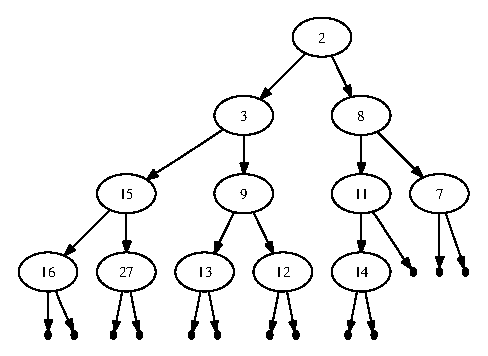
\epsfig{file=nearly-complete-tree.eps}
        \caption{Ein nahezu vollst�ndiger Baum der Tiefe 4.}
        \label{fig:nearly-complete-tree.eps}
      \end{figure}
      
      Stellen wir diesen Baum durch ein Feld dar, so erhalten wir das folgende Feld:
      \\[0.2cm]
      \hspace*{1.3cm}
      \texttt{[ 2, 3, 8, 15, 9, 11, 7, 16, 27, 13, 12, 14]} 
      \\[0.2cm]
      Dieses Feld entsteht aus dem vorigen Feld dadurch, dass wir die letzten drei
      Eintr�ge gel�scht haben.  Schlie�lich zeigt Abbildung
      \ref{fig:not-nearly-complete-tree.eps} auf Seite
      \pageref{fig:not-nearly-complete-tree.eps} noch einen bin�ren Baum, der nicht nahezu
      vollst�ndig ist, denn er enth�lt auf der untersten Ebene eine L�cke, weil die Knoten
      nicht von rechts nach links entfernt wurden.

      \begin{figure}[!ht]
        \centering
        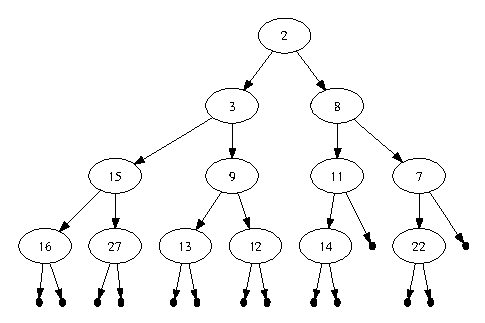
\epsfig{file=not-nearly-complete-tree.eps}
        \caption{Ein Baum, der nicht nahezu vollst�ndig ist.}
        \label{fig:not-nearly-complete-tree.eps}
      \end{figure}

      Bezeichnen wir die Menge der nahezu vollst�ndigen bin�ren B�ume mit $\Bin^*$, so
      k�nnen wir diese Menge formal durch eine Induktion definieren:
      \begin{enumerate}
      \item $n \in \overline{\Bin} \rightarrow n \in \Bin^*$,

            jeder vollst�ndige bin�re Baum ist nat�rlich erst recht nahezu vollst�ndig.
      \item $l \in \overline{\Bin} \wedge l.\textsl{height}() = h \wedge r \in \overline{\Bin}
             \wedge r.\textsl{height}() = h-1 \,\rightarrow\,
             \textsl{node}(k,v,l,r) \in \Bin^*$,

            falls $l$ ein vollst�ndiger bin�rer Baum der H�he $h$ ist und $r$ ein 
            vollst�ndiger bin�rer Baum der H�he $h-1$, dann ist
            $\textsl{node}(k,v,l,r)$ ein nahezu vollst�ndiger bin�rer Baum.
      \item $l \in \overline{\Bin} \wedge l.\textsl{height}() = h \wedge r \in \Bin^*
             \wedge r.\textsl{height}() = h \,\rightarrow\,
             \textsl{node}(k,v,l,r) \in \Bin^*$,

            falls $l$ ein vollst�ndiger bin�rer Baum der H�he $h$ ist und $r$ ein nahezu
            vollst�ndiger bin�rer Baum, der ebenfalls die H�he $h$ hat, dann ist
            $\textsl{node}(k,v,l,r)$ ein nahezu vollst�ndiger bin�rer Baum.

      \item $l \in \Bin^* \wedge l.\textsl{height}() = h \wedge r \in \overline{\Bin}
             \wedge r.\textsl{height}() = h-1 \,\rightarrow\,
             \textsl{node}(k,v,l,r) \in \Bin^*$,

            falls $l$ ein nahezu vollst�ndiger bin�rer Baum der H�he $h$ ist und $r$ ein 
            vollst�ndiger bin�rer Baum der H�he $h-1$ hat, dann ist
            $\textsl{node}(k,v,l,r)$ ein nahezu vollst�ndiger bin�rer Baum.
      \end{enumerate}
\end{enumerate}
Nahezu vollst�ndige bin�re B�ume lassen sich durch ein Feld darstellen, weil dann f�r
den linken und den rechten Teilbaum keine expliziten Referenzen abgespeichert werden
m�ssen.  Das spart Speicherplatz, die Implementierung ist aber etwas komplizierter als die
von uns entwickelte Variante.

Wir kommen nun zur�ck zur Diskussion der Klasse \texttt{PriorityQueue}.
Diese Klasse enth�lt die folgenden Konstruktoren.
\begin{enumerate}
\item \texttt{PriorityQueue()}

      Dieser Konstruktor erzeugt einen neue Priorit�ts-Warteschlange.
      Das zu Grunde liegende Feld hat dabei zun�chst die Gr��e 11.
      Wenn sp�ter der Platz in diesem Feld nicht mehr ausreicht, wird es dynamisch
      vergr��ert. 
\item \texttt{PriorityQueue(Collection<E> $c$)}
  
      Dieser Konstruktor erzeugt eine Priorit�ts-Warteschlange, die alle Elemente der
      Zusammenfassung $c$ enth�lt.
\item \texttt{PriorityQueue(int initialCapacity)}
  
      Dieser Konstruktor  erzeugt eine neue Priorit�ts-Warteschlange.
      Das zu Grunde liegende Feld hat dabei die Gr��e \texttt{initialCapacity}.
\item \texttt{PriorityQueue(int initialCapacity, Comparator<E> comparator)}

      Dieser Konstruktor  erzeugt einen neue Priorit�ts-Warteschlange.
      Das zu Grunde liegende Feld hat dabei die Gr��e \texttt{initialCapacity}.
      Die Elemente dieser Warteschlange werden nicht durch einen Aufruf der
      Methode 
      \\[0.2cm]
      \hspace*{1.3cm}
      $x.\texttt{compareTo}(y)$ 
      \\[0.2cm]
      verglichen, sondern statt dessen wird der als Argument �bergebene Comparator
      zum Vergleich benutzt:
      \\[0.2cm]
      \hspace*{1.3cm}
      $\mathtt{comparator}.\texttt{compare}(x,y)$. 
\end{enumerate}
Die Methoden, die zur Verf�gung gestellt werden, kennen wir schon aus unserer Diskussion
der Schnittstellen \texttt{Collection<E>} und \texttt{Queue<E>}. 
\begin{enumerate}
\item \texttt{boolean offer(E $e$)}

      Der Aufruf $q.\mathtt{offer}(e)$ f�gt das Element $e$ in die
      Priorit�ts-Warteschlange $q$ an und
      entspricht unserer Methode \textsl{insert}. 
\item \texttt{E peek()}

      Der Aufruf $q.\mathtt{peek}()$ liefert das Element mit der h�chsten Priorit�t in der
      Priorit�ts-Warte\-schlange $q$ als Ergebnis.   $q$ wird dabei nicht ver�ndert.  Falls $q$
      leer ist, wird \texttt{null} zur�ck gegeben.
\item \texttt{E poll()}

      Der Aufruf $q.\mathtt{poll}()$ liefert das Element mit der h�chsten Priorit�t in der
      Priorit�ts-Warte\-schlange $q$ als Ergebnis.  
      Das Element wird dabei aus $q$ entfernt.  Falls $q$
      leer ist, wird \texttt{null} zur�ck gegeben.
\item \texttt{boolean remove(E $e$)}

      Der Aufruf $q.\mathtt{remove}(e)$ entfernt das Element $e$ aus
      der Priorit�ts-Warteschlange $q$.  Falls $q$ das Element $e$ nicht enth�lt, bleibt
      $q$ unver�ndert.  In diesem Fall wird als Ergebnis \texttt{false} zur�ck gegeben,
      sonst wird \texttt{true} zur�ck gegeben.
\end{enumerate}
Die Klasse \texttt{PriorityQueue} enth�lt keine Methode, um die Priorit�t eines Elements
zu �ndern.  Das geht auch gar nicht, denn bei dieser Klasse wird nicht zwischen dem Wert
und dem Schl�ssel unterschieden, beide sind Teil eines Elements.  Um also einen Priorit�t
zu �ndern, m�ssen wir das betreffende Element zun�chst aus der Priorit�ts-Warteschlange
entfernen, die Priorit�t �ndern und anschlie�end das Element mit der ge�nderten Priorit�t
wieder einf�gen.


%\subsection{Repr\"asentierung von Heaps durch Listen}
Anstatt  Heaps durch bin\"are B\"aume zu repr\"asentieren, k\"onnen wir Heaps auch
durch Listen darstellen.   Die Idee ist, einen Heap durch eine  Liste der Form \\[0.1cm]
\hspace*{1.3cm} 
$L = \bigl[ \pair(k_1,v_1), \pair(k_2,v_2), \pair(k_3,v_3), \cdots, \pair(k_n,v_n) \bigr]$
\\[0.1cm]
zu repr\"asentieren.  Dazu m\"ussen wir zun\"achst festlegen, wie eine solche Liste als Heap
interpretiert werden kann.  Wir definieren daher eine Funktion \\[0.1cm]
\hspace*{1.3cm} 
$\textsl{interpret}: \textsl{List}\bigl((\textsl{Key}\times \textsl{Value})\cup \{\Omega\}\bigr) \times \mathbb{N}  \rightarrow \textsl{Heap}$
\\[0.1cm]
die eine Liste, deren Elemente entweder Paare von Priorit\"aten und Werten sind, oder aber
der spezielle Wert $\Omega$, in einem Heap umwandelt.  Die Funktion \textsl{interpret}
bekommt als zweites Argument einen Index, der in die Liste zeigt. Die Idee ist, dass der
Wert, der in der Liste unter diesem Index abgespeichert ist, die Wurzel des Baums
$\textsl{interpret}(L,i)$ markiert.  Bei der Definition von \textsl{interpret} gibt es zwei
F\"alle:
\begin{enumerate}
\item $L(i) = \Omega$.  Dann gilt nat\"urlich \ 
       $\textsl{interpret}(L,i) = \textsl{nil}$.
\item $L(i) = \pair(k, v)$. Dann gilt:\\[0.1cm]
      \hspace*{1.3cm} 
      $\textsl{interpret}(L,i) = \textsl{node}\bigl(k,v,\textsl{interpret}(L,2*i),\textsl{interpret}(L,2*i+1)\bigr)$.

      Die Idee bei dieser Definition ist es, dass der linke Sohn des durch den Index $i$
      repr\"asentierten Knotens an der Stelle $2*i$ abgespeichert wird, w\"ahrend der rechte
      Sohn unter dem Index $2*i + 1$ abgespeichert wird.
\end{enumerate}
Abbildung \ref{fig:heap-list} auf Seite \pageref{fig:heap-list} zeigt einen Heap, der die Zahlen $1, \cdots, 9$ als
Priorit\"aten enth\"alt.  Als Werte sind die Buchstaben ``\texttt{a}'', $\cdots$,
``\texttt{i}'' eingetragen.
  Als Liste repr\"asentiert hat dieser Heap die Form \\[0.1cm]
\hspace*{1.3cm} $L = \bigl[ \pair(1,\mathtt{a}), \pair(2,\mathtt{b}),
\pair(3,\mathtt{c}), \pair(4,\mathtt{d}), \pair(6,\mathtt{f}), 
\pair(5,\mathtt{e}), \pair(7,\mathtt{g}), \pair(8,\mathtt{h}), \Omega, \Omega,
\Omega, \pair(9, \mathtt{i}) \bigr]$.
\\[0.1cm]
Diese Liste hat gewissermassen L\"ocher, die durch die drei $\Omega$s repr\"asentiert
werden. Diese $\Omega$s entsprechen dem rechten Teilbaum des mit $4$ beschrifteten Knotens
und die beiden Teilb\"aume des mit $6$ beschrifteten Knotens.
Wollen wir Heaps durch Listen auf die oben skizzierte Weise implementieren, so brauchen wir au\3er der Liste $L$ noch
eine Liste \textsl{Counts}, wobei $\textsl{Counts}(i)$ die Zahl der Knoten in dem Teilbaum
angibt, dessen Wurzel an der Stelle $i$ in der Liste $L$ steht. 
Schlie\3lich ben\"otigen wir zur effizienten Implementierung der Methode $\textsl{change}()$
noch eine Funktion, die zu einem gegebenen Wert $v$ den Index $i$ berechnet, f\"ur den 
 $L(i) = \pair(k,v)$ \\[0.1cm]
gilt.  Wir realisieren diese Funktion in Form einer bin\"aren Relation.  Diese bin\"are
Relation speichern wir in der Instanz-Variablen \texttt{nodeIndex} ab.
Das folgende Listing zeigt die Listen-basierte Implementierung der Klasse \textsl{Heap}.

\begin{Verbatim}[ frame         = lines, 
                  framesep      = 0.3cm, 
                  labelposition = bottomline,
                  numbers       = left,
                  numbersep     = -0.2cm,
                  xleftmargin   = 0.8cm,
                  xrightmargin  = 0.8cm
                ]
    class body Heap;
   
        var L;
        var Counts;
        var nodeIndex;
   
        procedure create();
            L      := [];
            Counts := [];
            nodeIndex := {};
        end create;
   
        procedure insert(k, v);
            insertIndex(k, v, 1);
        end insert;
   
        procedure insertIndex(k, v, idx);
            if L(idx) = om then
                L(idx) := [ k, v ];
                Counts(idx) := 1;
                Counts(2 * idx) := 0;
                Counts(2 * idx + 1) := 0;
                nodeIndex(v) := idx;
                return;
            end if;
            Counts(idx) +:= 1;
            [ k1, v1 ] := L(idx);
            if k1 <= k then
                if Counts(2 * idx + 1) < Counts(2 * idx) then
                    insertIndex(k, v, 2 * idx + 1);
                else 
                    insertIndex(k, v, 2 * idx);
                end if;
                return;
            end if;
            L(idx) := [k, v];
            nodeIndex(v)  := idx;
            nodeIndex(v1) := om;
            if Counts(2 * idx + 1) < Counts(2 * idx) then
                insertIndex(k1, v1, 2 * idx + 1);
            else
                insertIndex(k1, v1, 2 * idx);
            end if;
        end insertIndex;
   
        procedure change(v, k);
            idx := nodeIndex(v);
            if idx = 1 then
                L(1) := [k, v];
            else
                parentIdx := idx / 2;
                [ kp, vp ] := L(parentIdx);
                if k < kp then
                    L(idx)       := [ kp, vp ];
                    L(parentIdx) := [ k, v ];
                    nodeIndex(vp) := idx;
                    nodeIndex(v)  := parentIdx;
                    change(v, k);
                else 
                    L(idx) := [ k, v ];
                end if;
            end if;
        end change;
   
        procedure top();
            return L(1);
        end top;
   
        procedure remove();
            removeIndex(1);
        end remove;
   
        procedure removeIndex(idx);
            if L(idx) = om then
                return;
            end if;
            Counts(idx) -:= 1;
            [k, v] := L(idx);
            nodeIndex(v) := om;
            if L(2 * idx) = om and L(2 * idx + 1) = om then
                L(idx) := om;
                Counts(2 * idx) := om;
                Counts(2 * idx + 1) := om;
                return;
            end if;
            if L(2 * idx) /= om and L(2 * idx + 1) = om then
                [k1, v1] := L(2 * idx);
                L(idx) := L(2 * idx);
                removeIndex(2 * idx);
                nodeIndex(v1) := idx;
                return;
            end if;
            if L(2 * idx) = om and L(2 * idx + 1) /= om then
                [k2, v2] := L(2 * idx + 1);
                L(idx) := L(2 * idx + 1);
                removeIndex(2 * idx + 1);
                nodeIndex(v2) := idx;
                return;
            end if;
            [ k1, v1 ] := L(2 * idx);
            [ k2, v2 ] := L(2 * idx + 1);
            if k1 <= k2 then
                L(idx) := [ k1, v1 ];
                removeIndex(2 * idx);
                nodeIndex(v1) := idx;
            else
                L(idx) := [ k2, v2 ];
                removeIndex(2 * idx + 1);
                nodeIndex(v2) := idx;
            end if;
        end removeIndex;
   
        procedure isEmpty();
            return L(1) = om;
        end isEmpty;
   
    end Heap;
\end{Verbatim}

%%% Local Variables: 
%%% mode: latex
%%% TeX-master: "algorithmen"
%%% End: 


%%% Local Variables: 
%%% mode: latex
%%% TeX-master: "algorithmen"
%%% End: 

\chapter{Daten-Kompression}
In diesem Kapitel untersuchen wir die Frage, wie wir einen gegebenen String $s$ m\"oglichst platzsparend
abspeichern k\"onnen.  Wir gehen davon aus, dass der String $s$ aus Buchstaben besteht, die 
Elemente einer Menge $\Sigma$ sind.  Die Menge $\Sigma$ bezeichnen wir als unser \emph{Alphabet}. 
Wenn das Alphabet aus $n$ verschiedenen Zeichen besteht und wir alle Buchstaben mit derselben L\"ange
von $b$ Bits kodieren wollen, dann muss f\"ur diese Zahl von Bits offenbar
\[ n \leq 2^b \] 
gelten, woraus
\[ b = \textsl{ceil}\bigl(\log_2(n)\bigr) \]
folgt.  Hier bezeichnet $\textsl{ceil}(x)$ die \emph{Ceiling-Funktion}.  Diese Funktion
rundet eine gegebene reelle Zahl immer auf, es gilt also
\[ \textsl{ceil}(x) = \min \{ k \in \N \mid x \leq k \}. \]
Besteht der String $s$ aus $m$ Buchstaben, so werden zur Kodierung des Strings insgesamt
$m \cdot b$ Bits gebraucht.  Nun gibt es zwei M\"oglichkeiten, weiterzumachen:
\begin{enumerate}
\item Lassen wir die Forderung, dass alle Buchstaben mit derselben Anzahl von Bits kodiert werden,
      fallen, dann ist es unter Umst\"anden m\"oglich, den String $s$ mit weniger Bits zu kodieren.  
      Dies f\"uhrt zu dem 1952 von David A.~Huffman angegebenen Algorithmus, den wir in den n\"achsten
      beiden Abschnitten vorstellen und analysieren.
\item Alternativ k\"onnen wir versuchen, Buchstabenkombinationen, die h\"aufig auftreten, als neue
      Buchstaben aufzufassen.  Beispielsweise kommen W\"orter wie ``\emph{der}'', ``\emph{die}'' und
      ``\emph{das}'' in deutschsprachigen Texten relativ h\"aufig vor.  Es ist daher sinnvoll, f\"ur
      solche Buchstaben-Kombinationen neue Codes einzuf\"uhren.  Ein Algorithmus, der auf dieser Idee
      basiert, ist der Lempel-Ziv-Welch Algorithmus, den wir im letzten Abschnitt dieses Kapitels 
      diskutieren werden.
\end{enumerate}


\section[Motivation]{Motivation des Algorithmus von Huffman}
Die zentrale Idee des von Huffman entwickelten Algorithmus ist die, dass Buchstaben, die sehr
h\"aufig auftreten, mit m\"oglichst wenig Bits kodiert werden, w\"ahrend Buchstaben, die seltener
auftreten, mit einer gr\"o{\ss}eren Anzahl Bits kodiert werden.  Zur Verdeutlichung betrachten
wir folgendes Beispiel:  Unser Alphabet  $\Sigma$ bestehe nur aus vier Buchstaben,
\[ \Sigma = \{ \mathtt{a}, \mathtt{b}, \mathtt{c}, \texttt{d} \}. \]
In dem zu speichernden String $s$ trete der Buchstabe \texttt{a} insgesamt $990$ mal auf, der
Buchstabe \texttt{b} trete $8$ mal auf und die Buchstaben \texttt{c} und \texttt{d} treten
jeweils $1$ mal auf.  Dann besteht der String $s$ aus insgesamt $1\,000$ 
Buchstaben.  Wenn wir jeden Buchstaben mit $2 = \log_2(4)$ Bits kodieren, dann werden also
insgesamt $2\,000$ Bits ben\"otigt um den String $s$ abzuspeichern.  Wir k\"onnen den String
aber auch mit weniger Bits abspeichern, wenn wir die einzelnen Buchstaben mit Bitfolgen
unterschiedlicher L\"ange kodieren.   In unserem konkreten
Beispiel wollen wir versuchen den Buchstaben \texttt{a}, der mit Abstand am h\"aufigsten
vorkommt, mit einem einzigen Bit zu kodieren.  Bei den  Buchstaben
\texttt{c} und \texttt{d}, die nur sehr selten auftreten, ist es kein Problem auch mehr
Bits zu verwenden.  Tabelle \ref{tab:coding} zeigt eine Kodierung, die von dieser Idee
ausgeht. 

\begin{table}[htbp]
  \centering
\begin{tabular}[t]{|l|r|r|r|r|}
\hline
Buchstabe  & \texttt{a} & \texttt{b}  & \texttt{c}   & \texttt{d}   \\
\hline
\hline
H\"aufigkeit &     990    &         8   &           1  &         1    \\
\hline
Kodierung  & \texttt{0} & \texttt{10} & \texttt{110} & \texttt{111} \\
\hline
\end{tabular}
  \caption{Kodierung der Buchstaben mit variabler L\"ange.}
  \label{tab:coding}
\end{table}

Um zu verstehen, wie diese Kodierung funktioniert, stellen wir sie in
Abbildung \ref{fig:coding-tree} als \emph{Kodierungs-Baum} dar.  Die inneren 
Knoten dieses Baums enthalten keine Attribute und werden als leere Kreise dargestellt.
Die Bl\"atter des Baums sind mit den Buchstaben markiert.
Die Kodierung eines Buchstabens ergibt sich \"uber die Beschriftung der Kanten, die von dem
Wurzel-Knoten zu dem Buchstaben f\"uhren.  Beispielsweise f\"uhrt von der Wurzel eine
Kante direkt zu dem Blatt, das mit dem Buchstaben ``\texttt{a}'' markiert ist.  Diese
Kante ist mit dem Label ``\texttt{0}'' beschriftet.  Also wird der Buchstabe
``\texttt{a}'' durch den String ``\texttt{0}'' kodiert.  Um ein weiteres Beispiel zu
geben, betrachten wir den Buchstaben ``\texttt{c}''.   Der Pfad, der von der Wurzel zu dem
Blatt f\"uhrt, das mit ``\texttt{c}'' markiert ist, enth\"alt drei Kanten.  Die ersten beiden
Kanten sind jeweils mit ``\texttt{1}'' markiert, die letzte Kante ist mit ``\texttt{0}''
markiert.  Also wird der Buchstabe ``\texttt{c}'' durch den String ``\texttt{110}''
kodiert.  Kodieren wir nun unseren urspr\"unglichen String $s$, der aus $990$
\texttt{a}'s, $8$ \texttt{b}'s, einem \texttt{c} und einem \texttt{d} besteht, so
ben\"otigen wir insgesamt
\[ 990 \cdot 1 + 8 \cdot 2 + 1 \cdot 3 + 1 \cdot 3 = 1\,012 \]
Bits.  Gegen\"uber der urspr\"unglichen Kodierung, die $2\,000$ Bits verwendet, haben wir $49,4\%$
gespart!

\begin{figure}[!ht]
  \centering
  \framebox{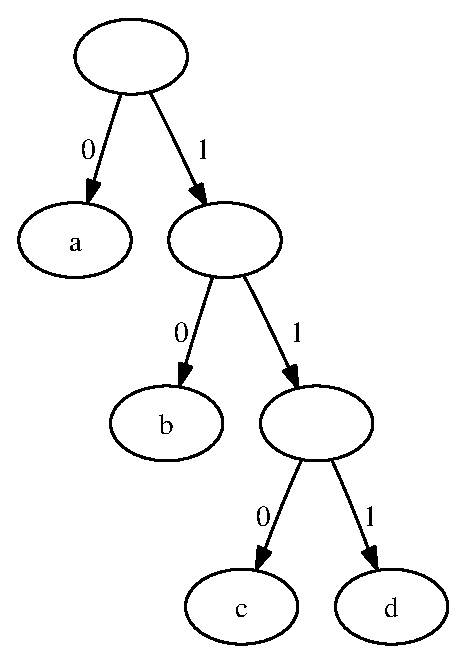
\epsfig{file=Abbildungen/coding-tree.eps, scale=0.5}} 
  \caption{Baum-Darstellung der Kodierung.}
  \label{fig:coding-tree}
\end{figure}

Um zu sehen, wie mit Hilfe des Kodierungs-Baums ein String dekodiert werden kann,
betrachten wir als Beispiel den String ``\texttt{100111}''.  Wir beginnen mit der
``\texttt{1}'', die uns sagt, vom Wurzel-Knoten dem rechten Pfeil zu folgen.  Die
anschlie{\ss}ende ``\texttt{0}'' spezifiziert dann den linken Pfeil.  Jetzt sind wir bei dem
mit ``\texttt{b}'' markierten Blatt angekommen und haben damit den ersten Buchstaben
gefunden.  Wir gehen wieder zur Wurzel des Baums zur\"uck. Die folgende ``\texttt{0}'' f\"uhrt
uns zu dem Blatt, das mit ``\texttt{a}'' markiert ist, also haben wir den zweiten
Buchstaben gefunden. Wir gehen wieder zur Wurzel zur\"uck.  Die Ziffern ``\texttt{111}''
f\"uhren uns nun zu dem Buchstaben ``\texttt{d}''.  Damit haben wir insgesamt
\\[0.2cm]
\hspace*{1.3cm}
``\texttt{100111}'' $\simeq$ ``\texttt{bad}''.


\section[Huffman's Algorithm]{Der Algorithmus von Huffman}
Angenommen, wir haben einen String $s$, der aus Buchstaben eines Alphabets $\Sigma$
aufgebaut ist.  Wie finden wir dann eine Kodierung f\"ur die einzelnen Buchstaben, die
mit m\"oglichst wenig Bits auskommt?  Der Algorithmus von Huffman gibt eine Antwort auf diese
Frage. Um diesen Algorithmus pr\"asentieren zu k\"onnen, definieren wir die Menge
$\mathcal{K}$ der \emph{Kodierungs-B\"aume} induktiv.  
\begin{enumerate}
\item $\textsl{Leaf}(c,f) \in \mathcal{K} \quad \mbox{falls $c \in \Sigma$ und $f \in \N$}$.

      Ausdr\"ucke der Form $\textsl{Leaf}(c,f)$ sind die Bl\"atter eines Kodierungs-Baums.
      Dabei ist $c$ ein Buchstabe aus unserem Alphabet $\Sigma$ und $f$ gibt die
      H\"aufigkeit an, mit der dieser Buchstabe in dem zu kodierenden String auftritt.

      Gegen\"uber Abbildung \ref{fig:coding-tree} kommen hier bei den Bl\"attern noch die
      H\"aufigkeiten hinzu.  Diese ben\"otigen wir, denn wir wollen ja sp\"ater Buchstaben,
      die sehr h\"aufig auftreten, mit m\"oglichst wenig Bits kodieren.  

\item $\textsl{Node}(l,r) \in \mathcal{K} \quad 
       \mbox{falls $l \in\mathcal{K}$ und $r \in \mathcal{K}$.}$ 

      Ausdr\"ucke der Form $\textsl{Node}(l,r)$ sind die inneren Knoten eines
      Kodierungs-Baums.  
\end{enumerate}
Als n\"achstes  definieren wir eine Funktion 
\[  \textsl{count} : \mathcal{K} \rightarrow \N, \]
welche die  Gesamt-H\"aufigkeiten aller in dem Baum auftretenden Buchstaben aufsummiert.
\begin{enumerate}
\item Die Definition der Funktion \textsl{count} ist f\"ur Bl\"atter trivial:
      \[ \textsl{Leaf}(c,f).\textsl{count}() = f. \]
\item Die Gesamt-H\"aufigkeit des Knotens $\textsl{Node}(l,r)$
      ergibt sich als Summe der Gesamt-H\"aufigkeiten von $l$ und $r$. Also gilt
      \[ \textsl{Node}(l,r).\textsl{count}() = l.\textsl{count}() + r.\textsl{count}(). \]
\end{enumerate}
Weiter definieren wir auf Kodierungs-B\"aumen die Funktion
\[ \textsl{cost}: \mathcal{K} \rightarrow \N. \]
Die Funktion \textsl{cost} gibt an, wie viele Bits ben\"otigt werden, um mit dem gegebenen
Kodierungs-Baum einen String zu kodieren, wenn die H\"aufigkeiten, mit denen ein Buchstabe
verwendet wird, mit den H\"aufigkeiten \"ubereinstimmen, die an den Bl\"attern des Baums notiert
sind.  Die Definition dieser Funktion ist induktiv:
\begin{enumerate}
\item $\textsl{Leaf}(c,f).\textsl{cost}() = 0$,

      denn solange nur ein einziger Buchstabe vorhanden ist, ist noch nichts zu kodieren.
\item $\textsl{Node}(l,r).\textsl{cost}() = 
       l.\textsl{cost}() + r.\textsl{cost}() + l.\textsl{count}() + r.\textsl{count}()$.

      Wenn wir zwei Kodierungs-B\"aume $l$ und $r$ zu einem neuen Kodierungs-Baum
      zusammenf\"ugen, verl\"angern sich die Kodierungen f\"ur alle Buchstaben, die in $l$ oder
      $r$ auftreten, um ein Bit.
      Die Summe 
      \[ l.\textsl{count}() + r.\textsl{count}() \]
      gibt die Gesamt-H\"aufigkeiten aller Buchstaben an, die in dem linken und
      rechten Teilbaum auftreten.  Da sich die Kodierung aller dieser Buchstaben
      durch die Bildung des Knotens $\textsl{Node}(l,r)$ gegen\"uber der Kodierung in $l$
      und $r$ jeweils um 1 verl\"angert, m\"ussen wir zu den Kosten der Teilb\"aume $l$ und $r$
      den Term $l.\textsl{count}() + r.\textsl{count}()$ hinzuaddieren.
\end{enumerate}
Wir erweitern die Funktion $\textsl{cost}()$ auf Mengen von Knoten, indem wir die Kosten
einer Menge $M$ als die Summe der Kosten der Knoten von $M$ definieren:
\[ \textsl{cost}(M) = \sum\limits_{n\in M} n.\textsl{cost}(). \]
Ausgangs-Punkt des von David A.~Huffman (1925 -- 1999) im Jahre 1952 angegebenen
Algorithmus \cite{huffman:52} ist eine Menge von Paaren der Form $\langle c, f\rangle$.  Dabei ist
$c$ ein 
Buchstabe und $f$ gibt die H\"aufigkeit an, mit der dieser Buchstabe auftritt.  Im ersten
Schritt werden diese Paare in die Bl\"atter eines Kodierungs-Baums \"uberf\"uhrt.  Besteht der
zu kodierende String aus  $n$ verschiedenen Buchstaben, so haben
wir dann eine Menge von Kodierungs-B\"aumen der Form
\begin{equation}
  \label{eq:huffmann1}
 M = \bigl\{  \textsl{Leaf}(c_1, f_1), \cdots, \textsl{Leaf}(c_k, f_k) \bigr\}   
\end{equation}
Es werden nun solange Knoten $a$ und $b$ aus $M$ zu einem neuen Knoten
$\textsl{Node}(a,b)$ zusammengefasst, bis die Menge $M$ nur noch einen Knoten enth\"alt.
Offenbar gibt es im Allgemeinen sehr viele M\"oglichkeiten, die Knoten aus der Menge zu
neuen Knoten zusammen zu fassen.  Das Ziel ist es die Knoten so zusammen zu fassen, dass
die Kosten der Menge $M$ am Ende  minimal sind.
Um zu verstehen, welche Knoten wir am geschicktesten zusammenfassen k\"onnen, betrachten wir, wie
sich die Kosten der Menge durch das Zusammenfassen zweier Knoten \"andert.
Dazu betrachten wir zwei Mengen von Knoten $M_1$ und $M_2$, so dass 
\[ M_1 = N \cup \{ a, b\} \quad \mathtt{und} \quad M_2 = N \cup \{ \textsl{Node}(a,b) \} \]
gilt, die Menge $M_1$ geht also aus der Menge $M_2$ dadurch hervor, dass wir
die Knoten $a$ und $b$ zu einem neuen Knoten zusammen fassen und durch diesen ersetzen.
Untersuchen wir, wie
sich die Kosten der Menge dabei ver\"andern, wir untersuchen also die folgende Differenz:
\begin{eqnarray*}
& & \textsl{cost}\bigl(N \cup \{ \textsl{Node}(a,b) \}\bigr) - \textsl{cost}\bigl(N \cup \{ a,b \}\bigr) \\
&=& \textsl{cost}\bigl( \{ \textsl{Node}(a,b) \}\bigr) - \textsl{cost}\bigl(\{ a,b \}\bigr)              \\
&=& \textsl{Node}(a,b).\textsl{cost}() - a.\textsl{cost}() - b.\textsl{cost}()                           \\
&=&   a.\textsl{cost}() + b.\textsl{cost}() + a.\textsl{count}() + b.\textsl{count}() 
    - a.\textsl{cost}() - b.\textsl{cost}()                                                              \\
&=& a.\textsl{count}() + b.\textsl{count}() 
\end{eqnarray*}
Fassen wir die Knoten $a$ und $b$ aus der Menge $M$ zu einem neuen Knoten zusammen, so verg\"o{\ss}ern sich
die Kosten der Menge um die Summe
\[ a.\textsl{count}() + b.\textsl{count}(). \]
Wenn wir die Kosten der Menge $M$ insgesamt m\"oglichst klein halten wollen, dann ist es daher naheliegend,
dass wir in der Menge $M$ die beiden Knoten $a$ und $b$ suchen, f\"ur die die Funktion
$\textsl{count}()$ den kleinsten Wert liefert.  Diese Knoten werden wir aus der Menge $M$
entfernen und durch den neuen Knoten $\textsl{Node}(a,b)$ ersetzen.
Dieser Prozess wird solange iteriert, bis die Menge $M$ nur noch aus einem Knoten besteht.  Dieser
Knoten ist dann die Wurzel des gesuchten Kodierungs-Baums. 

\begin{figure}[!ht]
\centering
\begin{Verbatim}[ frame         = lines, 
                  framesep      = 0.3cm, 
                  labelposition = bottomline,
                  numbers       = left,
                  numbersep     = -0.2cm,
                  xleftmargin   = 1.3cm,
                  xrightmargin  = 1.3cm,
                ]
    codingTree := procedure(m) {
        while (#m > 1) {
            a := first(m);
            m -= { a };
            b := first(m);
            m -= { b };
            m += { [ count(a) + count(b), Node(a, b) ] };
        }
        return arb(m);
    };    
    count := p |-> p[1];
\end{Verbatim}
\vspace*{-0.3cm}
\caption{Der Algorithmus von Huffman in \textsc{SetlX}.}
\label{fig:huffman.stlx}
\end{figure} % $

\noindent
Die in Abbildung \ref{fig:huffman.stlx} gezeigte Funktion $\mathtt{codingTree}(m)$
implementiert diesen Algorithmus. 
\begin{enumerate}
\item Die Funktion \textsl{codingTree} wird mit einer Menge $m$ von Knoten aufgerufen,
      welche die Form
      \\[0.2cm]
      \hspace*{1.3cm}
      $m = \bigl\{ \langle f_1, \textsl{Leaf}(c_1) \rangle, \cdots, 
                  \langle f_k, \textsl{Leaf}(c_k) \rangle \bigr\}   
      $
      \\[0.2cm]
      hat.  Hier bezeichnen die Variablen $c_i$ die verschiedenen Buchstaben, w\"ahrend die
      Zahl $f_i$ die H\"aufigkeit angibt, mit der der Buchstabe $c_i$ auftritt.

      Wir haben hier die Information \"uber die H\"aufigkeit an erster Stelle eines Paares gespeichert.
      Da \textsc{SetlX} diese Menge intern durch einen geordneten bin\"aren Baum
      abspeichert, erm\"oglicht uns diese Form der Darstellung einfach auf den Knoten mit
      der kleinsten H\"aufigkeit zuzugreifen, denn die Paare werden so verglichen, dass
      immer zun\"achst die erste Komponente zweier Paare zum Vergleich herangezogen werden.
      Nur wenn sich in der ersten Komponente kein Unterschied ergibt, wird auch die zweite
      Komponente verglichen.  Daher finden wir das Paar mit der kleinsten ersten
      Komponente immer am Anfang der Menge $m$.

      Durch diesen Trick haben wir uns de facto die Implementierung einer
      Priorit\"ats-Warteschlange gespart:  
      \begin{enumerate}
      \item Die in \textsc{SetlX} vordefinierte Funktion
            $\mathtt{first}(m)$ liefert das erste Element der Menge $m$ und entspricht
            damit der Funktion $\textsl{top}(m)$ des abstrakten Daten-Typs \textsl{PrioQueue}.
      \item Anstelle von $\textsl{insert}(m, p, v)$ k\"onnen wir einfach
            \\[0.2cm]
            \hspace*{1.3cm}
            \texttt{$m$ += \{ [$p$, $v$] \};}
            \\[0.2cm]
            schreiben um das Element $v$ mit der Priorit\"at $p$ in die
            Priorit\"ats-Warteschlange $m$ einzuf\"ugen.
      \item Die Funktion $\textsl{remove}(m)$ realisieren wir durch den Aufruf
            \\[0.2cm]
            \hspace*{1.3cm}
            \texttt{$m$ -= \{ first($m$) \};}
            \\[0.2cm]
            denn $\textsl{remove}(m)$ soll ja das Element mit der h\"ochsten Priorit\"at aus
            $m$ entfernen.
      \end{enumerate}
      Das Elegante an diesem Vorgehen ist, dass damit s\"amtliche Operationen des abstrakten
      Daten-Typs \textsl{PrioQueue} eine logarithmische Komplexit\"at haben.  Das ist zwar
      im Falle der Operation $\textsl{top}(m)$ nicht optimal, aber f\"ur die Praxis v\"ollig
      ausreichend, denn in der Praxis kommt auf jeden Aufruf der Form $\textsl{top}(m)$
      auch ein Aufruf der Form $\textsl{remove}(m)$ und der hat sowohl bei einer optimalen
      Implementierung als auch bei unserer Implementierung eine logarithmische
      Komplexit\"at, die dann auch im Falle der optimalen Implementierung  die gesamte
      Komplexit\"at dominiert. 
\item Die \texttt{while}-Schleife in Zeile 2 veringert die Anzahl der Knoten in der Menge $m$
      in jedem Schritt um Eins.  
      \begin{enumerate}
      \item Dazu werden mit Hilfe der Funktion $\textsl{first}()$ die
            beiden Knoten $a$ und $b$ berechnet, f\"ur die der Wert von $\textsl{count}()$ minimal
            ist.  Die Funktion $\mathtt{count}(p)$ ist in Zeile 11 definiert und liefert einfach die
            erste Komponente des Paares $p$, denn dort speichern wir die H\"aufigkeit der Buchstaben 
            ab.
      \item Die beiden Knoten $a$ und $b$ mit der geringsten H\"aufigkeit werden in Zeile 4 und 6
            aus der Menge $m$ entfernt.
      \item Anschlie{\ss}end wird aus den beiden Knoten $a$ und $b$ ein neuer Knoten 
            $\textsl{Node}(a,b)$ gebildet.
            Dieser neue Knoten wird zusammen mit der Gesamth\"aufigkeit der Knoten $a$ und $b$ in Zeile
            7 der Menge $m$ hinzugef\"ugt.
      \end{enumerate}
\item Die \texttt{while}-Schleife wird beendet, wenn die Menge $m$ nur noch ein Element enth\"alt.
      Dieses wird mit der Funktion \texttt{arb} extrahiert und als Ergebnis zur\"uck gegeben.
\end{enumerate}
Die Laufzeit des Huffman-Algorithmus h\"angt stark von der Effizienz der Funktion $\textsl{first}()$ ab.
Eine naive Implementierung w\"urde die Knoten aus der Menge $m$ in einer geordneten Liste vorhalten.
Die Knoten $n$ w\"aren in dieser Liste nach der Gr\"o{\ss}e $n.\textsl{cost}()$ aufsteigend sortiert.
Dann ist die Funktion $\textsl{first}()$ zwar sehr effizient, aber das Einf\"ugen des neuen Knotens,
dass wir oben \"uber den Befehl 
\\[0.2cm]
\hspace*{1.3cm}
\texttt{m += \{ [ count(a) + count(b), Node(a, b) ] \};}
\\[0.2cm]
realisieren,  w\"urde einen Aufwand erfordern, der linear in der Anzahl der Elemente der Menge $m$ ist.
Dadurch, dass wir mit einer Menge  $m$ arbeiten, die in \textsc{SetlX} intern durch einen
Rot-Schwarz-Baum dargestellt ist, erreichen wir, dass alle in der \texttt{while}-Schleife durchgef\"uhrten
Operationen nur logarithmisch von der Anzahl der Buchstaben abh\"angen.  Damit hat der Huffman-Algorithmus
insgesamt die Komplexit\"at $\Oh\bigl(n \cdot \ln(n)\bigr)$.
 

\begin{table}[htbp]
  \centering
\begin{tabular}[t]{|l|r|r|r|r|r|}
\hline
Buchstabe  & \texttt{a} & \texttt{b} & \texttt{c} & \texttt{d} & \texttt{e} \\
\hline
\hline
H\"aufigkeit &          1 &          2 &          3 &          4 &          5 \\
\hline
\end{tabular}
  \caption{Buchstaben mit H\"aufigkeiten.}
  \label{tab:frequency}
\end{table}

Wir illustrieren den  Huffman-Algorithmus, indem wir ihn auf die Buchstaben, die in
Tabelle \ref{tab:frequency} zusammen mit ihren H\"aufigkeiten angegeben sind, anwenden.
\begin{enumerate}
\item Zu Beginn hat die Menge $m$ die Form
      \\[0.2cm]
      \hspace*{0.3cm}
      $ m = \bigl\{ \langle 1, \textsl{Leaf}(\mathtt{a}) \rangle,\,
             \langle 2, \textsl{Leaf}(\mathtt{b}) \rangle,\, 
             \langle 3, \textsl{Leaf}(\mathtt{c}) \rangle,\,
             \langle 4, \textsl{Leaf}(\mathtt{d}) \rangle,\,
             \langle 5, \textsl{Leaf}(\mathtt{e}) \rangle\bigr\}. $
\item Die H\"aufigkeit ist hier f\"ur die Bl\"atter mit den Buchstaben \texttt{a} und
      \texttt{b} minimal.  Also entfernen wir diese Bl\"atter aus der Menge und f\"ugen statt
      dessen den Knoten 
      \\[0.2cm]
      \hspace*{0.3cm}
      $\textsl{Node}(\textsl{Leaf}(\mathtt{a}), \textsl{Leaf}(\mathtt{b}))$
      \\[0.2cm]
      in die Menge $m$ ein.  Die H\"aufigkeit dieses Knotens ergibt sich als Summe der H\"aufigkeiten
      der Buchstaben \texttt{a} und \texttt{b}. Daher f\"ugen wir insgesamt das Paar
      \\[0.2cm]
      \hspace*{0.3cm}
      $\langle 3, \textsl{Node}\bigl(\textsl{Leaf}(\mathtt{a}) \rangle, \textsl{Leaf}(\mathtt{b}) \bigr) \rangle$
      \\[0.2cm]
      in die Menge $m$ ein.        Dann hat $m$ die Form
      \\[0.2cm]
      \hspace*{0.3cm}
      $ \bigl\{\langle 3, \textsl{Leaf}(\mathtt{c}) \rangle,\,
			\langle 3, \textsl{Node}(\textsl{Leaf}(\mathtt{a}), \textsl{Leaf}(\mathtt{b}))\rangle,\,
              \langle 4, \textsl{Leaf}(\mathtt{d}) \rangle,\,
             \langle 5, \textsl{Leaf}(\mathtt{e}) \rangle\bigr\}. $
\item Die beiden Paare mit den kleinsten Werten der H\"aufigkeiten in $m$ sind nun
      \\[0.2cm]
      \hspace*{0.3cm}
      $ \langle 3, \textsl{Node}(\textsl{Leaf}(\mathtt{a}), \textsl{Leaf}(\mathtt{b})) \rangle
         \quad \mathrm{und} \quad \langle 3, \textsl{Leaf}(\mathtt{c})\rangle$.
      \\[0.2cm]
      Wir entfernen diese beiden Knoten und bilden aus diesen beiden Knoten den neuen Knoten
      \\[0.2cm]
      \hspace*{0.3cm}
      $ \langle 6, \textsl{Node}(
           \textsl{Node}((\textsl{Leaf}(\mathtt{a}), \textsl{Leaf}(\mathtt{b})),\; 
           \textsl{Leaf}(\mathtt{c}))\rangle, $
      \\[0.2cm]
      den wir der Menge $m$ hinzuf\"ugen.  Dann hat $m$ die Form
      \\[0.2cm]
      \hspace*{0.3cm}
      $ \Bigl\{ 
        \langle 4, \textsl{Leaf}(\mathtt{d}) \rangle,\;\langle 5, \textsl{Leaf}(\mathtt{e}) \rangle,\;
        \langle 6, \textsl{Node}(
           \textsl{Node}(\textsl{Leaf}(\mathtt{a}), \textsl{Leaf}(\mathtt{b})),\; 
           \textsl{Leaf}(\mathtt{c}))\Bigr\}. $
\item Jetzt sind 
      \\[0.2cm]
      \hspace*{0.3cm}
      $ \langle 4, \textsl{Leaf}(\mathtt{d}) \rangle \quad \mathrm{und} \quad \langle 5, \textsl{Leaf}(\mathtt{e}) \rangle$
      \\[0.2cm]
      die beiden Knoten mit dem kleinsten Werten der H\"aufigkeit.
      Wir entfernen diese Knoten und bilden den neuen Knoten \\[0.2cm]
      \hspace*{0.3cm}
      $\langle 9, \textsl{Node}(\textsl{Leaf}(\mathtt{d}), \textsl{Leaf}(\mathtt{e})) \rangle$.
      \\[0.2cm]
      Diesen f\"ugen wir der Menge $m$ hinzu und erhalten
      \\[0.2cm]
      \hspace*{0.3cm}
      $ \Bigl\{ 
        \langle 6, \textsl{Node}(
           \textsl{Node}(\textsl{Leaf}(\mathtt{a}),
           \textsl{Leaf}(\mathtt{b})),\,\textsl{Leaf}(\mathtt{c},3))
        \rangle,\;
        \langle 9,\textsl{Node}(\textsl{Leaf}(\mathtt{d},4), \textsl{Leaf}(\mathtt{e},5)) \rangle
        \Bigr\}
           $.      
\item Jetzt enth\"alt die Menge $m$ nur noch zwei Knoten.  Wir entfernen diese beiden Knoten und
      bilden daraus den neuen Knoten
      \\[0.2cm]
      \hspace*{0.3cm}
      $\textsl{Node}\biggl(
              \textsl{Node}\Bigl(
                 \textsl{Node}\bigl(\textsl{Leaf}(\mathtt{a}), \textsl{Leaf}(\mathtt{b})\bigr),\; 
                 \textsl{Leaf}(\mathtt{c})\Bigr),\;
              \textsl{Node}\bigl(\textsl{Leaf}(\mathtt{d}), \textsl{Leaf}(\mathtt{e})\bigr)
         \biggr)
      $
      \\[0.2cm]
      Dieser Knoten ist jetzt der einzige Knoten in $m$ und damit unser Ergebnis.
      Stellen wir diesen Knoten als Baum dar, so erhalten wir das in Abbildung
      \ref{fig:coding-tree2} gezeigte Ergebnis.  Wir haben hier jeden Knoten $n$
      mit dem Funktionswert  $n.\textsl{count}()$ beschriftet.  

      Die Kodierung, die sich daraus ergibt,
      wird in Tabelle \ref{tab:coding2} gezeigt.
\end{enumerate}

\begin{figure}[!ht]
  \centering
  \framebox{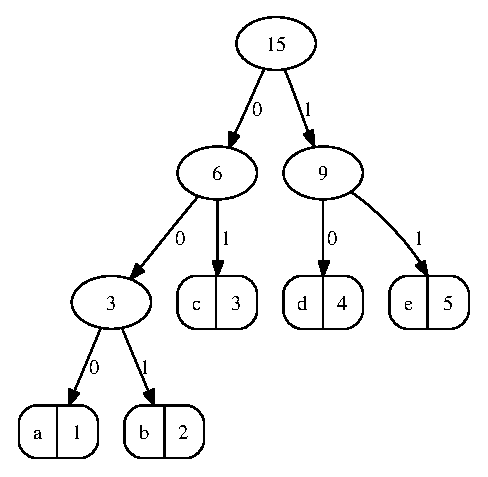
\epsfig{file=Abbildungen/coding-tree2.eps, scale=0.7}} 
  \caption{Baum-Darstellung der Kodierung.}
  \label{fig:coding-tree2}
\end{figure}



\begin{table}[htbp]
  \centering
\begin{tabular}[t]{|l|r|r|r|r|r|}
\hline
Buchstabe &   \texttt{a} &   \texttt{b} & \texttt{c}  & \texttt{d}  & \texttt{e}   \\
\hline
\hline
Kodierung & \texttt{000} & \texttt{001} & \texttt{01} & \texttt{10} & \texttt{11} \\
\hline
\end{tabular}
  \caption{Kodierung der Buchstaben mit variabler L\"ange.}
  \label{tab:coding2}
\end{table}


\exercise
\begin{enumerate}[(a)]
\item Berechnen Sie den Huffman-Code f\"ur einen Text, der nur die Buchstaben
      ``\texttt{a}'' bis ``\texttt{g}'' enth\"alt und f\"ur den die H\"aufigkeiten,
      mit denen diese Buchstaben auftreten, durch die folgende Tabelle gegeben sind.

\begin{table}[htbp]
  \centering
\begin{tabular}[t]{|l|r|r|r|r|r|r|r|}
\hline
Buchstabe  & \texttt{a} & \texttt{b} & \texttt{c} & \texttt{d} & \texttt{e} & \texttt{f} & \texttt{g} \\
\hline
\hline
H\"aufigkeit &          1 &          1 &          2 &          3 &          5 &         8 &         13 \\
\hline
\end{tabular}
  \caption{Buchstaben mit H\"aufigkeiten.}
  \label{tab:aufgabe-huffman}
\end{table}

\item Wie gro{\ss} ist die Einsparung, wenn man die Buchstaben mit einem Huffman-Code
      kodiert gegen\"uber einer Kodierung mit drei Bits?
\item Versuchen Sie das Gesetz zu erkennen, nach dem die H\"aufigkeiten in der obigen Tabelle 
      gebildet wurden und versuchen Sie, den Huffman-Code f\"ur den allgemeinen Fall,
      in dem $n$ Buchstaben gegeben sind, anzugeben.
\item Wie gro{\ss} ist die Einsparung im allgemeinen Fall?
\end{enumerate}


\section[LZW Algorithm]{The Algorithm  of Lempel, Ziv, and Welch}
The algorithm developed by Abraham Lempel, Jacob Ziv \cite{ziv:77,ziv:78} and Terry A.~Welch
\cite{welch:84}, which is also known as the \emph{LZW algorithm}, is based on the idea that in most
texts certain combinations of letters are quite frequent.  Therefore, it should pay of to view
these combinations of letters as new letters and insert them into the alphabet.  This is the main
idea of the LZW algorithm.  However, since counting the occurrences of all words would be too time
consuming, the LZW algorithm works with a \emph{dynamic} coding dictionary.  Initially, this dictionary
contains only the \textsc{Ascii} characters.  Then, the idea is to extend this dictionary
dynamically: Every time a new string is encountered, it is entered into the dictionary and a code is
assigned to the corresponding string.  However, since it would not make sense to add arbitrary
strings to the dictionary, a new string $s$ of length $n=\#s$ is only added to the dictionary if
\begin{enumerate}
\item $s$ is a substring of the string that is encoded and
\item the substring $s[1..n-1]$ has already been entered into the dictionary.  
\end{enumerate} 
The algorithm is best
explained via an example.  The basic working of the algorithm is explained with the help of four
variables:
\begin{enumerate}
\item $\alpha$ is the last substring that has been encoded.  Initially, this is the empty string
      $\varepsilon$.
  
      The encoding of a string $s$ by the LZW algorithm works by encoding substrings of $s$ as
      numbers and $\alpha$ denotes the last of theses substrings.
\item $c$ is the next character of the string that is inspected.  This is also know as the
      \emph{look-ahead character}.
\item \textsl{d} ist the dictionary mapping strings to numbers.  Initially, \textsl{d} maps all
      \textsc{Ascii} characters to their respective \textsc{Ascii} codes.
\item \texttt{nextCode} is the number assigned as code to the next string that is entered into
      the dictionary $d$.  Since the \textsc{Ascii} codes are the numbers from 0 up to 127,
      initially \texttt{nextCode} is equal to $128$.
\end{enumerate}
To describe the working of the algorithm, let us encode the string ``\texttt{maumau}''.
\begin{enumerate}
\item Initially, we have
      \\[0.2cm]
      \hspace*{1.3cm}
      $\alpha = \varepsilon$ \quad and \quad $c = \mathtt{m}$.
      \\[0.2cm]
      Since the \textsc{Ascii} code of the character ``\texttt{m}'' is $109$, we output this number.
\item After reading the next character ``\texttt{a}'' we have
      \\[0.2cm]
      \hspace*{1.3cm}
      $\alpha = \mathtt{m}$ \quad and \quad $c = \mathtt{a}$.
      \\[0.2cm]
      Now, the substring $\alpha c$, which is ``\texttt{ma}'', is entered into the dictionary and
      assigned to the code $128$:
      \\[0.2cm]
      \hspace*{1.3cm}
      $d = d \cup \{\langle \mathtt{ma}, 128 \rangle\}$.
      \\[0.2cm]
      Furthermore, we output the \textsc{Ascii} code of ``\texttt{a}'', which is $97$.
\item After reading the next character ``\texttt{u}'' we have
      \\[0.2cm]
      \hspace*{1.3cm}
      $\alpha = \mathtt{a}$ \quad and \quad $c = \mathtt{u}$.
      \\[0.2cm]
      Now, the substring $\alpha c$, which is ``\texttt{au}'', is entered into the dictionary and
      assigned to the next available code, which is $129$:
      \\[0.2cm]
      \hspace*{1.3cm}
      $d = d \cup \{\langle \mathtt{au}, 129 \rangle\}$.
      \\[0.2cm]
      Furthermore, we output the \textsc{Ascii} code of ``\texttt{u}'', which is $117$.
\item After reading the next character, which is the character ``\texttt{m}'', we have
      \\[0.2cm]
      \hspace*{1.3cm}
      $\alpha = \mathtt{u}$ \quad and \quad $c = \mathtt{m}$.
      \\[0.2cm]
      Next, the substring $\alpha c$, which is ``\texttt{um}'', is entered into the dictionary and
      assigned to the next available code, which is $130$:
      \\[0.2cm]
      \hspace*{1.3cm}
      $d = d \cup \{\langle \mathtt{um}, 130 \rangle\}$.
      \\[0.2cm]
      Since our dictionary already contains the substring ``\texttt{ma}'' and the character
      ``\texttt{a}'' is indeed the character following the character ``\texttt{m}'', we output
      $128$, which is the code assigned to the string ``\texttt{ma}''.

\item The next character to be read is now the final character ``\texttt{u}''.  We have
      \\[0.2cm]
      \hspace*{1.3cm}
      $\alpha = \mathtt{ma}$ \quad and \quad $c = \mathtt{u}$.
      \\[0.2cm]
      Next, the substring $\alpha c$, which is ``\texttt{mau}'', is entered into the dictionary and
      assigned to the next available code, which is $131$:
      \\[0.2cm]
      \hspace*{1.3cm}
      $d = d \cup \{\langle \mathtt{mau}, 131 \rangle\}$.
      \\[0.2cm]
      Furthermore, we output the \textsc{Ascii} code of ``\texttt{u}'', which is $117$.
\end{enumerate} 
Putting everything together, we have coded the string ``\texttt{maumau}'' as the list
\\[0.2cm]
\hspace*{1.3cm}
$[109,97,117,128,117]$
\\[0.2cm]
If we had encoded this string in \textsc{Ascii} we would have used $6 \cdot 7 = 42$ bits.  Since the
dictionary that we have built on the fly uses codes starting at 128 we now have to use 8 bits to
encode the numbers.  However, we have only used 5 numbers to encode the string ``\texttt{maumau}''.
Hence we have only used $5 \cdot 8 = 40$ bits.   Of course, in this tiny example the compression
factor is quite low.  However, for texts that are longer and have more repetitions, the compression
factor is usually higher: On average, the experience shows that text corresponding to natural
language is compressed by a factor that is sightly bigger than $2$.

If we use the LZW algorithm there is no need to add the dictionary to the encoded string.  The
reason is that the recipient of an encoded string can construct the dictionary using exactly the
algorithm that is used when encoding the string.

Let us summarize the algorithm seen in the previous example:
\begin{enumerate}
\item The dictionary is initialized to map all \textsc{Ascii} characters to their \textsc{Ascii} codes.
\item Next, we search for the longest prefix $\beta$ of $s$ that is in the dictionary.  This prefix
      is removed from $s$.
\item We emit the code stored for $\beta$ in the dictionary.
\item Let $\alpha$ be the string that has been encoded in the previous step.  Append the first
      character $c$ of $\beta$ to $\alpha$ and enter the resulting string $\alpha c$ to the
      dictionary.

      This step expands the dictionary dynamically.
\item Go to step 2 and repeat as long as the string $s$ is not empty.
\end{enumerate}
Decoding a list of numbers $l$ into a string $s$ is quite similar to the encoding and works as follows.
\begin{enumerate}
\item This time, the dictionary is initialized to map all \textsc{Ascii} codes to their corresponding
      \textsc{Ascii} characters.  Hence, the dictionary constructed in this step is just the inverse
      of the dictionary constructed when starting to encode the string.
\item We initialize $s$ as the 
      empty string, which is denoted as $\varepsilon$:
      \\[0.2cm]
      \hspace*{1.3cm}
      $s := \varepsilon$.
\item We remove the first number $n$ from the list $l$ and look up the corresponding
      string $\beta$ in the dictionary.  This string is appended to $s$.
\item Assume that $\alpha$ is the string decoded in the previous iteration and that $c$ is the first
      character of $\beta$.  Enter the resulting string $\alpha c$ into the dictionary.
\item Goto step 2 and repeat as long as the list $l$ is not empty.
\end{enumerate}
The third step of this algorithm needs to refined:  The problem is
that it might happen that the dictionary does not have an entry for the number $n$.  This can occur because
the encoder is one step ahead of the decoder: The encoder encodes a substring and enters a code
corresponding to the previous substring into the dictionary.  Now if the next substring is identical
to the substring just entered, the encoder will produce a code that is not yet in the dictionary of
the decoder when he tries to decode it.   The question then is: How do we decode a number that has
not yet been entered into the dictionary.  To answer this question, we can reason an follows:
If the encoder outputs a code that it has just entered into the dictionary, then the string that is
encoded starts with the string that has been output previously, followed by some character.  However,
this character must be the first character of the string encoded now.  The string encoded now
corresponds to the code and hence this string is the same as the string previously decoded plus one
character. Therefore, if the previous string is $\alpha$, then the string
corresponding to an unknown code must be $\alpha \alpha[1]$, i.e. $\alpha$ followed by the first
character of $\alpha$.



\subsection{Implementing the LZW algorithm in \textsc{SetlX}}
In order to gain a better understanding of a complex algorithm it is best to code this algorithm.
Then the resulting program can be run on several examples.  Since humans tend
to learn better from examples than from logical reasoning, inspecting these examples deepens
the understanding of the algorithm.  We proceed to discuss an implementation of the LZW
algorithm.  

\begin{figure}[!ht]
\centering
\begin{Verbatim}[ frame         = lines, 
                  framesep      = 0.3cm, 
                  firstnumber   = 1,
                  labelposition = bottomline,
                  numbers       = left,
                  numbersep     = -0.2cm,
                  xleftmargin   = 0.8cm,
                  xrightmargin  = 0.8cm,
                ]
    class lzw() {
        mDictionary := { [ char(i), i ] : i in [32 .. 127] };
        mInverse    := { [ i, char(i) ] : i in [32 .. 127] };
        mNextCode   := 128;
    
        static {
            compress      := procedure(s)     { ... };
            uncompress    := procedure(l)     { ... };
            longestPrefix := procedure(s, i)  { ... };
        }
    }
\end{Verbatim}
\vspace*{-0.3cm}
\caption{Outline of the class \texttt{lzw}.}
\label{fig:lzw.stlx-outline}
\end{figure}


Figure \ref{fig:lzw.stlx-outline} shows the outline of the class \texttt{lzw}.  This class contains both the
method \texttt{compress} that takes a string $s$ and encodes this string into a list of numbers
and the method \texttt{uncompress} that takes a list of numbers $l$ and decodes this list back into
a string $s$.  These methods are designed to satisfy the following specification:
\\[0.2cm]
\hspace*{1.3cm}
$l = \mathtt{lzw().compress}(s_1) \wedge s_2 = \mathtt{lzw().uncompress}(l) \rightarrow s_1 = s_2$.
\\[0.2cm]
Furthermore, the class \texttt{lzw} contains the auxiliary method \texttt{longestPrefix}, which will
be discussed later.  The class \texttt{lzw} contains 3 member variables:
\begin{enumerate}
\item \texttt{mDictionary} is the dictionary used when encoding a string.  It is initialized to map
      the \textsc{Ascii} characters to their codes.  Remember that for a given number $i$, the
      expression $\mathtt{char}(i)$ returns the \textsc{Ascii} character with code $i$.
\item \texttt{mInverse} is a binary relation that associates the codes with the corresponding
      strings.  It is initialized to map every number in the set $\{ 0, 1, 2, \cdots, 127 \}$
      with the corresponding \textsc{Ascii} character.  The binary relation \texttt{mInverse} is the
      inverse of the relation \texttt{mDictionary}.
\item \texttt{mNextCode} gives the value of the next code used in the dictionary.  Since the codes
      up to and including $127$ are already used for the \textsc{Ascii} character, the next
      available code will be $128$.
\end{enumerate}

\begin{figure}[!ht]
\centering
\begin{Verbatim}[ frame         = lines, 
                  framesep      = 0.3cm, 
                  firstnumber   = 1,
                  labelposition = bottomline,
                  numbers       = left,
                  numbersep     = -0.2cm,
                  xleftmargin   = 0.8cm,
                  xrightmargin  = 0.8cm,
                ]
    compress := procedure(s) {
        result := [];
        idx    := 1;
        while (idx <= #s) {
            p := longestPrefix(s, idx);
            result += [ mDictionary[s[idx..p]] ];
            if (p < #s) {
                mDictionary[s[idx..p+1]] := mNextCode;
                this.mNextCode += 1;
            }
            idx := p + 1;
        }
        return result;
    };
\end{Verbatim}
\vspace*{-0.3cm}
\caption{The method \texttt{compress} encodes a string as a list of integers.}
\label{fig:lzw.stlx-compress}
\end{figure}
Figure \ref{fig:lzw.stlx-compress} shows the implementation of the method compress.  We discuss this
implementation line by line.
\begin{enumerate}
\item The variable \texttt{result} points to the list that encodes the string $s$ given as argument.
      Initially, this list is empty.  Every time a substring of $s$ is encoded, the corresponding code
      is appended to this list.
\item The variable \texttt{idx} is an index into the string $s$.  The idea is that the substring
      $s[1..\mathtt{idx}-1]$ has been encoded and the corresponding codes have already been written
      to the list \texttt{result}, while the substring $s[\mathtt{idx}..]$ is
      the part of $s$ that still needs to be encoded.
\item Hence, the \texttt{while}-loop runs as long as the index \texttt{idx} is less or equal than
      the length $\texttt{\#}s$ of the string $s$.
\item Next, the method \texttt{longestPrefix}  computes the index of longest prefix of the substring
      $s[\mathtt{idx}..]$ that can be found in the dictionary \texttt{mDictionary}, i.e.~$p$ is the
      maximal number such that the expression \texttt{mDictionary[s[idx..p]]} is defined.
\item The code corresponding to this substring is looked up in \texttt{mDictionary}
      and is then appended to the list \texttt{result}.
\item Next, we take care to maintain the dictionary \texttt{mDictionary} and add the substring
      $s[\mathtt{idx}..p+1]$ to the dictionary.  Of course, we can only do this if the upper index
      of this expression, which is $p+1$, is an index into the string $s$. 
      Therefore we have to check that $p < \mathtt{\#}s$.
      Once we have entered the
      new string with its corresponding code into the dictionary, we have to make sure that the
      variable \texttt{mNextCode} is incremented so that every string is associated with a unique
      code.  
\item Since the code corresponding to the substring $s[\mathtt{idx}..p]$ has been written to the
      list \texttt{result}, the index \texttt{idx} is set to $p+1$.
\item Once the while loop has terminated, the string $s$ has been completely encoded and the list
      containing the codes can be returned.
\end{enumerate}


\begin{figure}[!ht]
\centering
\begin{Verbatim}[ frame         = lines, 
                  framesep      = 0.3cm, 
                  firstnumber   = 1,
                  labelposition = bottomline,
                  numbers       = left,
                  numbersep     = -0.2cm,
                  xleftmargin   = 0.8cm,
                  xrightmargin  = 0.8cm,
                ]
    longestPrefix := procedure(s, i) {
       oldK := i;
       k    := i+1;
       while (k <= #s && mDictionary[s[i..k]] != om) {
           oldK := k;
           k    += 1;
       }
       return oldK;
    };
    incrementBitNumber := procedure() {
        if (2 ** mBitNumber <= mNextCode) {
            this.mBitNumber += 1;
        }
    };
\end{Verbatim}
\vspace*{-0.3cm}
\caption{Computing the longest prefix.}
\label{fig:lzw.stlx-longestPrefix}
\end{figure}
Figure \ref{fig:lzw.stlx-longestPrefix} show the implementation of the auxiliary function
\texttt{longestPrefix}.  
The function $\texttt{longestPrefix}(s, i)$ computes the maximum value of $k$ such that
\\[0.2cm]
\hspace*{1.3cm}
$i \leq k \wedge k \leq \texttt{\#}s \wedge \mathtt{mDictionary}[s[i..k]] \not= \Omega$.
\\[0.2cm]
This value is well defined since the dictionary is initialized to contain all strings of
length 1.  Therefore, $\texttt{mDictionary}[s[i..i]]$ is known to be defined: It is the
\textsc{Ascii} code of the character $s[i]$.
      
The required value is computed by a simple \texttt{while}-loop that tests all possible values of $k$.
The loop exits once the value of $k$ is too big.  Then the previous value of $k$, which is
stored in the variable \texttt{oldK} is returned as the result.




\begin{figure}[!ht]
\centering
\begin{Verbatim}[ frame         = lines, 
                  framesep      = 0.3cm, 
                  firstnumber   = 1,
                  labelposition = bottomline,
                  numbers       = left,
                  numbersep     = -0.2cm,
                  xleftmargin   = 0.8cm,
                  xrightmargin  = 0.8cm,
                ]
    uncompress := procedure(l) {
        result := "";
        idx    := 1;
        code   := l[idx]; 
        old    := mInverse[code];
        idx    += 1;
        while (idx < #l) {
            result += old;
            code := l[idx];
            idx  += 1;
            next := mInverse[code];
            if (next == om) {
                next := old + old[1];
            }
            mInverse[mNextCode] := old + next[1];
            this.mNextCode += 1;
            old := next;
        }
        result += old;
        return result;
    };
\end{Verbatim}
\vspace*{-0.3cm}
\caption{The method \texttt{uncompress} to decode a list of integers into a string.}
\label{fig:lzw.stlx-uncompress}
\end{figure}
Figure \ref{fig:lzw.stlx-uncompress} shows the implementation of the method \texttt{uncompress} that
takes a list of numbers and decodes it into a string $s$.
\begin{enumerate}
\item The variable \texttt{result} contains the decoded string.  Initially, this variable is empty.
      Every time a code of the list $l$ is deciphered into some string, this string is added to
      \texttt{result}.
\item The variable \texttt{idx} is an index into the list $l$.  It points to the next code that
      needs to be deciphered.
\item The variable \texttt{code} contains the code in $l$ at position \texttt{idx}.  Therefore, we
      always have
      \\[0.2cm]
      \hspace*{1.3cm}
      $l[\mathtt{idx}] = \mathtt{code}$
\item The variable \texttt{old} contains the substring associated with \texttt{code}.  Therefore,
      the invariant
      \\[0.2cm]
      \hspace*{1.3cm}
      $\texttt{mInverse}[\mathtt{code}] = \mathtt{old}$
      \\[0.2cm]
      is maintained.
\item As long as the index \texttt{idx} still points inside the list, the substring 
      that has just been decoded is appended to the string \texttt{result}.
\item Then, an attempt is made to decode the next number in the list $l$ by looking up the code
      in the dictionary \texttt{mInverse}.  
      
      Now there is one subtle case: If the \texttt{code} has not yet been defined in the
      dictionary,  then we can conclude that this code has been created when coding the
      substring \texttt{old} followed by some character $c$.  However, as the next substring $\beta$
      corresponds to this code, the character $c$ must be the first
      character of this substring, i.e.~we have
      \\[0.2cm]
      \hspace*{1.3cm}
      $c = \beta[1]$.
      \\[0.2cm]
      On the other hand, we know that the substring $\beta$ has the form
      \\[0.2cm]
      \hspace*{1.3cm}
      $\beta = \mathtt{old} + c$,
      \\[0.2cm]
      where the operator ``$+$'' denotes string concatenation.  But then the first character of this string
      must be the first character of \texttt{old}, i.e.~we have
      \\[0.2cm]
      \hspace*{1.3cm}
      $\beta[1] = \mathtt{old}[1]$
      \\[0.2cm]
      and hence we have shown that
      \\[0.2cm]
      \hspace*{1.3cm}
      $c = \mathtt{old}[1]$.
      \\[0.2cm]
      Therefore, we conclude
      \\[0.2cm]
      \hspace*{1.3cm}
      $\beta = \mathtt{old} + \mathtt{old}[1]$
      \\[0.2cm]
      and hence this is the string encoded by a code that is not yet defined in the dictionary
      \texttt{mInverse}.
\item Next, we need to maintain the dictionary \texttt{mInverse} in the same fashion as the
      dictionary \texttt{mDictionary} is maintained in the method \texttt{compress}:
      Hence we take the string previously decoded and concat the next character of the
      string decoded in the current step.  Of course, this string is
      \\[0.2cm]
      \hspace*{1.3cm}
      $\texttt{old} + \mathtt{next}[1]$
      \\[0.2cm]
      and this string is then associated with the next available code value.
\item At the end of the loop, we need to set \texttt{old} to \texttt{next} so that \texttt{old}
      will always contain the string decoded in the previous step.
\item When the \texttt{while}-loop has terminated, we still need to append the final value of \texttt{old}
      to the variable \texttt{result}.
\end{enumerate}
Now that we have discussed the implementation of the \texttt{LZW} algorithm I would like to
encourage you to test it on several examples that are not too long.  Time does not permit me
to discuss examples of this kind in these lecture notes and, indeed, I do not think that discussing
these examples here would be as beneficial for the student as performing the algorithm on their own.

\exercise
\begin{enumerate}[(a)]
\item Use the LZW algorithm to encode the string ``\texttt{abcabcabcabc}''.  Compute the compression
      factor for this string.
\item For all $n \in \mathbb{N}$ with $n \geq 1$ the string $\alpha_n$ is defined inductively as
      follows:
      \\[0.2cm]
      \hspace*{1.3cm} $\alpha_1 := \mathtt{a}$ \quad and \quad $\alpha_{n+1} = \alpha_n + \mathtt{a}$.
      \\[0.2cm]
      Hence, the string $\alpha_n$ has the form $\underbrace{\mathtt{a} \cdots \mathtt{a}}_n$,
      i.e. it is the character \texttt{a} repeated $n$ times.
      Encode the string $\alpha_n$ using the LZW algorithm.  What is the compression rate?
\item Decode the list 
      \\[0.2cm]
      \hspace*{1.3cm}
      $[97, 98, 128, 130]$
      \\[0.2cm]
      using the LZW algorithm.  \eox
\end{enumerate}

%%% Local Variables: 
%%% mode: latex
%%% TeX-master: "algorithms"
%%% End: 

\chapter{Graph Theory}
In this chapter we are going to discuss three problems from \blue{graph theory}.
\begin{enumerate}
\item We present an algorithm to solve the 
      \href{https://en.wikipedia.org/wiki/Disjoint-set_data_structure}{\emph{union-find problem}}.
      In this problem, we are given a set $M$ and a relation $R \subseteq M \times M$.  Our task is
      then to find the \blue{equivalence relation} that is \blue{generated} by $R$.  The equivalence relation
      generated by the relation $R$ is the \blue{smallest equivalence relation} $\approx_R$ such that $R \subseteq\; \approx_R$.
      
      Essentially, the union-find problem is a mathematical problem.  Nevertheless, we will see that 
      it has an important practical application in computer science. 
\item The next problem we solve is the problem to compute the
      \href{https://en.wikipedia.org/wiki/Minimum_spanning_tree}{\emph{minimum spanning tree}}
      of a graph.  Given a weighted graph, this problem asks to find the smallest 
      \href{https://en.wikipedia.org/wiki/Glossary_of_graph_theory_terms#subgraph}{subgraph} that 
      connects all vertices of the graph.  We discuss
      \href{https://en.wikipedia.org/wiki/Kruskal%27s_algorithm}{Kruskal's algorithm} 
      for solving this problem.  
\item Then we discuss the problem of finding a shortest path in a 
      \href{https://en.wikipedia.org/wiki/Directed_graph}{\emph{weighted directed graph}}.
      We present \href{https://en.wikipedia.org/wiki/Dijkstra%27s_algorithm}{Dijkstra's algorithm} to solve
      this problem.   
\item Finally, we discuss \blue{topological sorting}.
\end{enumerate}

\section{The Union-Find Problem}
Assume that we are given a set $M$ together with a relation $R \subseteq M \times M$.  The relation
$R$ is not yet an  \href{https://en.wikipedia.org/wiki/Equivalence_relation}{equivalence relation} on $M$, but
this relation \blue{generates} an equivalence relation $\approx_R$ on $M$.  This
\blue{generated equivalence relation} is defined inductively. 
\begin{enumerate}
\item For every pair $\pair(x,y) \in R$ we have that $\pair(x, y) \in\; \approx_R$.

      This is the base case of the inductive definition.  It ensures that the relation
      $\approx_R$ is an \blue{extension} of the relation $R$, i.e.~it ensures that $R \subseteq\, \approx_R$.
\item For every $x \in M$ we have $\pair(x,x) \in\; \approx_R$.

      This ensures that the relation $\approx_R$ is \blue{reflexive} on $M$.
\item If $\pair(x,y) \in \approx_R$, then $\pair(y,x) \in\; \approx_R$.

      This  ensures that the relation $\approx_R$ is \blue{symmetric}.
\item If $\pair(x,y) \in\; \approx_R$ and $\pair(y,z) \in\; \approx_R$, then $\pair(x,z) \in\; \approx_R$.

      This clause ensures that the relation $\approx_R$ is \blue{transitive}.
\end{enumerate}
Given this inductive definition, it can be shown that:
\begin{enumerate}
\item $\approx_R$ is an equivalence relation on $M$.
\item If $Q$ is an equivalence relation on $M$ such that $R \subseteq Q$, then $\approx_R \subseteq Q$.
\end{enumerate}
Therefore, the relation $\approx_R$ is the \blue{smallest}
equivalence relation on $M$ that extends $R$.  In our lesson on
\href{https://github.com/karlstroetmann/Lineare-Algebra/blob/master/Skript/lineare-algebra.pdf}{Linear Algebra}
we had defined the transitive closure $R^+$ of a binary relation $R$ in a similar way.  In 
that lecture, we had then shown that $R^+$ is indeed the smallest transitive relation that extends
$R$.  This proof can easily be adapted to prove the claim given above.

It turns out that a direct implementation of the inductive definition of $\approx_R$ given above is
not very efficient.  Instead, we remind ourselves that there is are one-to-one correspondence
between the equivalence relations $R \subseteq M \times M$ and the
\href{https://en.wikipedia.org/wiki/Partition_of_a_set}{partitions} of $M$.  A set 
$\mathcal{P} \subseteq 2^M$ is a \blue{partition} of $M$ iff the following holds:
\begin{enumerate}
\item $\{\} \not\in \mathcal{P}$,
\item $A \in \mathcal{P} \wedge B \in \mathcal{P} \rightarrow A = B \vee A \cap B = \{\}$,
\item $\ds\bigcup \mathcal{P} = M$.
\end{enumerate}
Therefore, a partition $\mathcal{P}$ of $M$ is a subset of the power set of $M$ such that
every element of $M$ is a member of \magenta{exactly one} set of $\mathcal{P}$ and, furthermore, $\mathcal{P}$ must not contain the
empty set.  We have already seen in the lecture on Linear Algebra that an equivalence relation 
$\approx \;\subseteq M \times M$ gives rise to
\href{https://en.wikipedia.org/wiki/Equivalence_class}{equivalence classes}, 
where the \blue{equivalence class} generated by $x \in M$ is defined as
\\[0.2cm]
\hspace*{1.3cm}
$[x]_\approx := \{ y \mid \pair(x, y) \in\; \approx \}$.
\\[0.2cm]
It was then shown that the set 
\\[0.2cm]
\hspace*{1.3cm}
$\bigl\{ [x]_\approx \;\big|\; x \in M \bigr\}$
\\[0.2cm]
is a partition of $M$.  It was also shown that every partition $\mathcal{P}$ of a set $M$ gives rise
to an equivalence relation $\approx_\mathcal{P}$ that is defined as follows:
\\[0.2cm]
\hspace*{1.3cm}
$x \approx_\mathcal{P} y \;\Longleftrightarrow\; \exists A \in \mathcal{P}:(x \in A \wedge y \in A)$.
\\[0.2cm]
An example will clarify the idea.  Assume that
\\[0.2cm]
\hspace*{1.3cm}
$M := \{ 1,2,3,4,5,6,7,8,9 \}$.
\\[0.2cm]
Then the set 
\\[0.2cm]
\hspace*{1.3cm}
$\mathcal{P} := \bigl\{ \{ 1, 4, 7, 9\}, \{3, 5, 8\}, \{2, 6\} \bigr\}$
\\[0.2cm]
is a partition of $M$ since the three sets involved are disjoint and their union is the set $M$.
According to this partition, the elements $1$, $4$, $7$, and $9$ are all
equivalent to each other.  Similarly, the elements $3$, $5$, and $8$ are equivalent to each other,
and, finally, $2$ and $6$ are equivalent.

It turns out that, given a relation $R$, the most efficient way to compute the generated equivalence
relation $\approx_R$ is to compute the partition corresponding to this equivalence relation.  In
order to present the algorithm, we first sketch the underlying idea using a simple example.  Assume
the set $M$ is defined as
\\
\hspace*{1.3cm}
$M := \{ 1,2,3,4,5,6,7,8,9 \}$
\\[0.2cm]
and that the relation $R$ is given as follows:
\\[0.2cm]
\hspace*{1.3cm}
$R := \bigl\{ \pair(1,4), \pair(7,9), \pair(3,5), \pair(2,6), \pair(5,8), \pair(1,9), \pair(4,7) \bigr\}$.
\\[0.2cm]
Our goal is to compute a partition $\mathcal{P}$ of $M$ such that the formula
\\[0.2cm]
\hspace*{1.3cm}
$\pair(x, y) \in R \rightarrow \exists A \in \mathcal{P}:\bigl(x \in A \wedge y \in A)$
\\[0.2cm]
holds.  In order to achieve this goal, we define a sequence of partitions $\mathcal{P}_1$,
$\mathcal{P}_2$, $\cdots$, $\mathcal{P}_n$ such that $\mathcal{P}_n$ achieves our goal.
\begin{enumerate}
\item We start by defining
      \\[0.2cm]
      \hspace*{1.3cm}
      $\mathcal{P}_1 := \bigl\{ \{1\}, \{2\}, \{3\}, \{4\}, \{5\}, \{6\}, \{7\}, \{8\}, \{9\} \bigr\}$.
      \\[0.2cm]
      This is clearly a partition of $M$, but it is the trivial one since it generates an equivalence
      relation $\approx$ where we have  $x \approx y$ if and only if $x = y$.  
\item Next, we have to ensure to incorporate our given relation $R$ into this partition.  Since $\pair(1,4) \in R$
      we replace the singleton sets $\{1\}$ and $\{4\}$ by their union.  This leads to the following
      definition of the partition $\mathcal{P}_2$:
      \\[0.2cm]
      \hspace*{1.3cm}
      $\mathcal{P}_2 := \bigl\{ \{1, 4\}, \{2\}, \{3\}, \{5\}, \{6\}, \{7\}, \{8\}, \{9\} \bigr\}$.
\item Since $\pair(7,9) \in R$, we replace the sets $\{7\}$ and $\{9\}$ by their union and define
      \\[0.2cm]
      \hspace*{1.3cm}
      $\mathcal{P}_3 := \bigl\{ \{1, 4\}, \{2\}, \{3\}, \{5\}, \{6\}, \{7, 9\}, \{8\} \bigr\}$.
\item Since $\pair(3,5) \in R$, we replace the sets $\{3\}$ and $\{5\}$ by their union and define
      \\[0.2cm]
      \hspace*{1.3cm}
      $\mathcal{P}_4 := \bigl\{ \{1, 4\}, \{2\}, \{3,5\}, \{6\}, \{7, 9\}, \{8\} \bigr\}$.
\item Since $\pair(2,6) \in R$, we replace the sets $\{2\}$ and $\{6\}$ by their union and define
      \\[0.2cm]
      \hspace*{1.3cm}
      $\mathcal{P}_5 := \bigl\{ \{1, 4\}, \{2,6\}, \{3,5\}, \{7, 9\}, \{8\} \bigr\}$.
\item Since $\pair(5,8) \in R$, we replace the sets $\{3,5\}$ and $\{8\}$ by their union and define
      \\[0.2cm]
      \hspace*{1.3cm}
      $\mathcal{P}_6 := \bigl\{ \{1, 4\}, \{2,6\}, \{3,5,8\}, \{7, 9\} \bigr\}$
\item Since $\pair(1,9) \in R$, we replace the sets $\{1,4\}$ and $\{7,9\}$ by their union and define
      \\[0.2cm]
      \hspace*{1.3cm}
      $\mathcal{P}_7 := \bigl\{ \{1, 4, 7, 9\}, \{2,6\}, \{3,5,8\} \bigr\}$
\item Next, we have $\pair(4,7) \in R$.  However, $4$ and $7$ are already in the same set.
      Therefore we do not have to change the partition $\mathcal{P}_7$ in this step.
      Furthermore, we have now processed all the pairs in the given relation $R$.
      Therefore, $\mathcal{P}_7$ is the partition that represents the equivalence relation $\approx$ generated
      by $R$.  According to this partition, we have found that
      \\[0.2cm]
      \hspace*{1.3cm}
      $1 \approx 4 \approx 7 \approx 9$, \quad $2 \approx 6$,  \quad and \quad $3 \approx 5 \approx 8$.
\end{enumerate}
 
\begin{figure}[!ht]
\centering
\begin{minted}[ frame         = lines, 
                framesep      = 0.3cm, 
                firstnumber   = 1,
                bgcolor       = sepia,
                numbers       = left,
                numbersep     = -0.2cm,
                xleftmargin   = 0.8cm,
                xrightmargin  = 0.8cm,
                ]{python3}
     def union_find(M, R):
        P = { frozenset({x}) for x in M } 
        for x, y in R:
            Sx = find(x, P)
            Sy = find(y, P)
            if Sx != Sy:
                P -= { Sx,  Sy }
                P |= { Sx | Sy }
        return P
    
    def arb(S):
        for x in S: return x
    
   def find(x, P):
        return arb({ S for S in P if x in S })    
\end{minted}
\vspace*{-0.3cm}
\caption{A naive implementation of the union-find algorithm.}
\label{fig:Union-Find-Naive.ipynb}
\end{figure}


What we have sketched in the previous example is known as the \blue{union-find algorithm}.
Figure \ref{fig:Union-Find-Naive.ipynb} shows a naive implementation of this algorithm.  The
procedure $\texttt{unionFind}$ takes two arguments: $\texttt{M}$ is a set and $\texttt{R}$ is a relation
on $\texttt{M}$.  The purpose of $\texttt{unionFind}$ is to compute the equivalence relation $\approx_\texttt{R}$
that is generated by $\texttt{R}$ on $M$.  This equivalence relation is represented as a partition of $\texttt{M}$.
\begin{enumerate}
\item In line 2 we initialize $\texttt{P}$ as the trivial partition that contains only singleton
      sets.  Obviously, this is a partition of $\texttt{M}$ but it does not yet take the
      relation $\texttt{R}$ into account.
\item The \texttt{for}-loop in line 3 iterates over all pairs $(\texttt{x},\texttt{y})$ from $\texttt{R}$.
      First, we compute the set $\texttt{Sx}$ that contains $\texttt{x}$ and the set $\texttt{Sy}$ that
      contains $\texttt{y}$.  If these sets are not the same, then $\texttt{x}$ and $\texttt{y}$ are not
      yet equivalent with respect to the partition $\texttt{p}$.  Therefore, the equivalence classes
      $\texttt{Sx}$ and $\texttt{Sy}$ are joined and their union is added to the partition 
      $\texttt{P}$ in line 8, while the equivalence classes $\texttt{Sx}$ and $\texttt{Sy}$ are
      removed from $\texttt{P}$ in line 7.
\item The function \texttt{arb} takes a set $S$ as its argument and returns an
      arbitrary element from $S$. 
\item The function $\texttt{find}$ takes an element $\texttt{x}$ of a set $\texttt{M}$ and a partition
      $\texttt{P}$ of $\texttt{M}$.  Since $\texttt{P}$ is a partition of $\texttt{M}$ there must be exactly
      one set $\texttt{S}$ in $\texttt{P}$ such that $\texttt{x}$ is an element of $\texttt{S}$.  This set
      $\texttt{S}$ is then returned.
\end{enumerate}

\subsection{A Tree-Based Implementation}
The implementation shown in Figure \ref{fig:Union-Find-Naive.ipynb} is not very efficient.  The
problem is the computation of the union
\\
\hspace*{1.3cm}
$\texttt{Sx} + \texttt{Sy}$.
\\[0.2cm]
If the sets $\texttt{Sx}$ and $\texttt{Sy}$ are represented as binary trees and, for the sake of the
argument, the set $\texttt{Sx}$ contains at most as many elements as the set $\texttt{Sy}$, then the
computational complexity of this operation is
\\
\hspace*{1.3cm}
$\Oh\bigl(\texttt{\#Sx} \cdot \log_2(\texttt{\#Sy})\bigr)$.  
\\[0.2cm]
The reason is that every element of $\texttt{Sx}$ has to be inserted into $\texttt{Sy}$ and this
insertion has a complexity of $\Oh\bigl(\log_2(\#\texttt{Sy})\bigr)$.  Here the expression
$\texttt{\#Sx}$ denotes the size of the set $\texttt{Sx}$ and similarly the expression
$\texttt{\#Sy}$ denotes the size of the set $\texttt{Sy}$.  A more efficient way to
represent these sets is via \blue{parent pointers}:  The idea is that every set is represented as a
tree.  However, this tree is not a binary tree but is rather represented by pointers that
point from a node to its parent.  The node at the root of the tree points to itself.  Then, taking the
union of two sets $\texttt{Sx}$ and $\texttt{Sy}$ is straightforward:  If $\texttt{rx}$ is the node at the root of
the tree representing $\texttt{Sx}$ and $\texttt{ry}$ is the node at the root of the tree representing
$\texttt{Sy}$, then changing the parent pointer of $\texttt{ry}$ to point to $\texttt{rx}$ merges the
sets \texttt{Sx} and \texttt{Sy}.


\begin{figure}[!ht]
\centering
\begin{minted}[ frame         = lines, 
                framesep      = 0.3cm, 
                firstnumber   = 1,
                bgcolor       = sepia,
                numbers       = left,
                numbersep     = -0.2cm,
                xleftmargin   = 0.8cm,
                xrightmargin  = 0.8cm,
              ]{python3}
    def find(x, Parent):
        if Parent[x] == x:
            return x
        return find(Parent[x], Parent)

    def union_find(M, R):
        Parent = { x: x for x in M } 
        for x, y in R:
            root_x = find(x, Parent)
            root_y = find(y, Parent)
            if root_x != root_y:
                Parent[root_y] = root_x
        Roots = { x for x in M if Parent[x] == x }
        return [{y for y in M if find(y, Parent) == r} for r in Roots]
\end{minted}
\vspace*{-0.3cm}
\caption{A tree-based implementation of the union-find algorithm.}
\label{fig:Union-Find-Tree.ipynb}
\end{figure}

Figure \ref{fig:Union-Find-Tree.ipynb} on page \pageref{fig:Union-Find-Tree.ipynb} shows an
implementation of this idea.  In this implementation, the parent pointers are represented using the
binary relation $\texttt{Parent}$.  
\begin{enumerate}
\item The function $\texttt{find}$ takes a node $\texttt{x}$ and the dictionary $\texttt{Parent}$ 
      that represents the parent pointers.  For a node $\texttt{y}$ the expression
      $\texttt{Parent}[\texttt{y}]$ returns the parent node of \texttt{y}.
      The purpose of the call $\texttt{find}(\texttt{x}, \texttt{Parent})$ is to
      return the root of the tree containing $\texttt{x}$.

      If $\texttt{x}$ is its own parent, then $\texttt{x}$ is already at the root of a tree and therefore 
      we can return $\texttt{x}$ itself in line 3.
      Otherwise, we compute the parent of $\texttt{x}$ and then recursively compute the root of the tree
      containing this parent.  
\item The function $\texttt{unionFind}$ takes a set $\texttt{M}$ and a relation $\texttt{R}$.  It returns
      a partition of $\texttt{M}$ that represents the equivalence relation generated by $\texttt{R}$ on
      $\texttt{M}$.  As I did not want to use \texttt{frozenset}s, this partition is represented by a list of
      sets. 

      The dictionary\footnote{
        In a language like \texttt{C} we would instead use pointers.  Of course, this would be more efficient.
      } $\texttt{Parent}$ is initialized in line 8 so that every node
      points to itself.   This corresponds to the fact that the sets in the initial partition are all
      singleton sets.  

      Next, the function $\texttt{unionFind}$ iterates over all pairs $[\texttt{x}, \texttt{y}]$ from the binary
      relation $\texttt{R}$.  In line 9 and 10 we compute the roots of the trees containing $\texttt{x}$ and
      $\texttt{y}$.  If these roots are identical, then $\texttt{x}$ and $\texttt{y}$ are already
      equivalent and there is nothing to do.  However, if $\texttt{x}$ and $\texttt{y}$ are located 
      in different trees, then these trees need to be merged.  To this end, the parent pointer of
      the root of the tree containing $\texttt{y}$ is changed so that it 
      points to the root of the tree containing $\texttt{x}$.  Therefore, instead of iterating over all
      elements of the set containing $\texttt{y}$, we just change a single pointer.

      Line 13 computes the set of all nodes that are at the root of some tree.  Then, for every root
      $\texttt{R}$ of a tree, line 14 computes the set of nodes corresponding to this tree.
      These sets are collected in a list, which is then returned.
\end{enumerate}

\subsection{Controlling the Growth of the Trees}
As it stands, the algorithm shown in the previous section has a complexity that is $\Oh(n^2)$ in the
worst case where $n$ is the number of elements in the set $ \texttt{M}$.  The worst case happens if there
is just one equivalence class and the tree representing this class degenerates into a list.
Fortunately, it is easy to fix this problem if we keep track of the \magenta{height} of the
different trees.  Then, if we want to join the trees rooted at $\texttt{parentX}$ and
$\texttt{parentY}$, we have a choice: We can either set the parent of the node $\texttt{parentX}$ to
be $\texttt{parentY}$ or we can set the parent of the node $\texttt{parentY}$ to be $\texttt{parentX}$.
If the tree rooted at $\texttt{parentX}$ is smaller than the tree rooted at $\texttt{parentY}$, then we should
use the assignment
\\[0.2cm]
\hspace*{1.3cm}
\texttt{parent[parentX] := parentY;}
\\[0.2cm]
otherwise we should use
\\[0.2cm]
\hspace*{1.3cm}
\texttt{parent[parentY] := parentX;}
\\[0.2cm]
In order to be able to distinguish these cases, we store the height of the tree rooted at node
$\texttt{n}$ in the relation $\texttt{Height}$, i.e.~if $\texttt{n}$ is a node, then $\texttt{Height}[\mathtt{n}]$ is
the height of the tree rooted at node $\texttt{n}$.  This yields the implementation shown in Figure
\ref{fig:Union-Find.ipynb} on page \pageref{fig:Union-Find.ipynb}.  Provided the size  of the relation
$\texttt{R}$ is bounded by the size $n$ of the set $ \texttt{M}$, the complexity of this
implementation is $\Oh\bigl(n \cdot \log(n)\bigr)$.  However, this excludes the last two lines of
the program.  In practice, the implementation of the function $\texttt{unionFind}$ would omit these
two lines and, instead, return the relation $\texttt{Parent}$ since this is all that is needed to
determine whether two elements $x$ and $y$ are equivalent. 

\begin{figure}[!ht]
\centering
\begin{minted}[ frame         = lines, 
                framesep      = 0.3cm, 
                firstnumber   = 1,
                bgcolor       = sepia,
                numbers       = left,
                numbersep     = -0.2cm,
                xleftmargin   = 0.0cm,
                xrightmargin  = 0.0cm,
              ]{python3}
    def union_find(M, R):
        Parent = { x: x for x in M } 
        Height = { x: 1 for x in M }
        for x, y in R:
            root_x = find(x, Parent)
            root_y = find(y, Parent)
            if root_x != root_y:
                if Height[root_x] < Height[root_y]:
                    Parent[root_x] = root_y
                elif Height[root_x] > Height[root_y]:
                    Parent[root_y] = root_x
                else:
                    Parent[root_y]  = root_x
                    Height[root_x] += 1
        Roots = { x for x in M if Parent[x] == x }
        return [{y for y in M if find(y, Parent) == r} for r in Roots]
\end{minted}
\vspace*{-0.3cm}
\caption{A more efficient version of the union-find algorithm.}
\label{fig:Union-Find.ipynb}
\end{figure}

\exercise
We can speed up the implementation previously shown if the set $\texttt{M}$ has the form
\\[0.2cm]
\hspace*{1.3cm}
$\texttt{M} = \{ 0, 1, 2, \cdots, n-1 \}$ \quad where $n \in \mathbb{N}$.
\\[0.2cm]
In this case, the relations $\texttt{Parent}$ and $\texttt{Height}$ can be implemented as arrays.
Develop an implementation that is based on this idea.
\eox

\subsection{Packaging the  Union-Find Algorithm as a Class \label{sec:union-find-oo}}
When we later discus  the minimum spanning tree problem,  we will need the union-find algorithm as an
auxiliary data structure.  To this end we present a class that encapsulates the union-find
algorithm.  This class is shown in Figure \ref{fig:Union-Find-OO.ipynb} on page
\pageref{fig:Union-Find-OO.ipynb}.

\begin{figure}[!ht]
\centering
\begin{minted}[ frame         = lines, 
                framesep      = 0.3cm, 
                firstnumber   = 1,
                bgcolor       = sepia,
                numbers       = left,
                numbersep     = -0.2cm,
                xleftmargin   = 0.0cm,
                xrightmargin  = 0.0cm,
              ]{python3}
    class UnionFind:
        def __init__(self, M):
            self.mParent = { x: x for x in M }
            self.mHeight = { x: 1 for x in M }
            
        def find(self, x):
            if self.mParent[x] == x:
                return x
            return find(self, self.mParent[x])
        
        def union(self, x, y):
            root_x = self.find(x)
            root_y = self.find(y)
            if root_x != root_y:
                if self.mHeight[root_x] < self.mHeight[root_y]:
                    self.mParent[root_x] = root_y
                elif self.mHeight[root_x] > self.mHeight[root_y]:
                    self.mParent[root_y] = root_x
                else:
                    self.mParent[root_y]  = root_x
                    self.mHeight[root_x] += 1
                    
    def partition(M, R):
        UF = UnionFind(M)
        for x, y in R:
            UF.union(x, y)
        Roots = { x for x in M if UF.find(x) == x }
        return [{y for y in M if UF.find(y) == r} for r in Roots]
\end{minted}
\vspace*{-0.3cm}
\caption{The class \texttt{unionFind}.}
\label{fig:Union-Find-OO.ipynb}
\end{figure}

\begin{enumerate}
\item The constructor $\texttt{unionFind}$ receives a set $\texttt{M}$ as arguments.  The class
      $\texttt{unionFind}$ maintains two variables:
      \begin{enumerate}
      \item $\texttt{mParent}$ is the dictionary implementing the pointers that point to the parents
             of each node.  If a node $\texttt{n}$ has no parent, then we have
             \\[0.2cm]
             \hspace*{1.3cm}
             \texttt{mParent[n] = n},
             \\[0.2cm]
             i.e.~the roots of the trees point to themselves.  Initially, all nodes are roots, so
             all parent pointers point to themselves.
      \item $\texttt{mHeight}$ is a dictionary containing the heights of the trees.  If $\texttt{n}$ is
            a node, then
            \\[0.2cm]
            \hspace*{1.3cm}
            \texttt{mHeight[n]}
            \\[0.2cm]
            gives the height of the subtree rooted at $\texttt{n}$. As initially all trees contain but
            a single node, these trees all have height $1$.
      \end{enumerate}
\item The method $\texttt{union}$ takes two nodes $\texttt{x}$ and $\texttt{y}$ and joins the trees that
      contain these nodes.  This is achieved by finding their parents $\texttt{parentX}$ and
      $\texttt{parentY}$.  Then, the root of the smaller of the two trees is redirected to point to
      the root of the bigger tree.
\item The method $\texttt{find}$ takes a node $\texttt{x}$ as its argument and computes the root of the
      tree containing $\texttt{x}$. 
\item The function $\texttt{partition}$ is a client of the class $\texttt{unionFind}$.  It takes a set
      $\texttt{M}$ and a relation $\texttt{R}$ on $\texttt{M}$ and computes a partition that corresponds
      to the equivalence relation generated by $\texttt{R}$ on $\texttt{M}$. 
      \begin{enumerate}
      \item First, the function constructs a union-find object $\texttt{uf}$ for the set $\texttt{M}$.
      \item Then the method iterates over all pairs $[\texttt{x},\texttt{y}]$ in the relation $\texttt{R}$ and
            joins the equivalence classes corresponding to $\texttt{x}$ and $\texttt{y}$.
      \item Next, the method collects all nodes $\texttt{x}$ that are at the root of a tree.
      \item Finally, for every root $\texttt{R}$ the method collects those nodes $\texttt{x}$ that are
            part of the tree rooted at $\texttt{R}$.
      \end{enumerate}
\end{enumerate}


\section{Minimum Spanning Trees}
Imagine a telecommunication company that intends to supply internet access to a developing country.
The capital of the country is located at the coast line and is already connected to the internet via
a submarine cable. It is the company's task to connect all of the towns and villages to the capital.
Since most parts of the country are covered by jungle, it is cheapest to build the power lines
alongside existing roads.  Mathematically, this kind of problem can be formulated as the problem of
constructing a \href{https://en.wikipedia.org/wiki/Minimum_spanning_tree}{minimum spanning tree} for
a given \href{https://en.wikipedia.org/wiki/Graph_(discrete_mathematics)#Weighted_graph}{weighted}
\href{https://en.wikipedia.org/wiki/Graph_(discrete_mathematics)#Undirected_graph}{undirected graph}.
Next, we provide the definitions of those notions that are needed to formulate the minimum spanning
tree problem precisely.  Then, we present
\href{https://en.wikipedia.org/wiki/Kruskal%27s_algorithm}{Kruskal's algorithm} for solving the
minimum spanning tree problem. 

\subsection{Basic Definitions}
\begin{Definition}[Weighted Graph] A \blue{weighted undirected graph} is a triple 
   $\langle \nodes, \edges, \weight{\cdot} \rangle$ such that
  \begin{enumerate}
  \item $\nodes$ is the set is a set of  \blue{nodes}.
  \item $\edges$ is the set of  \blue{edges}.  An edge $e$ has the form
        \\[0.2cm]
        \hspace*{1.3cm}
        $\{x, y\}$
        \\[0.2cm]
        and connects $x$ and $y$.  Since $\{x,y\}$ is a set, we have
        \\[0.2cm]
        \hspace*{1.3cm}
        $\{x,y\} \in \edges$ \quad if and only if $\{y,x\} \in \edges$.
        \\[0.2cm]
        Hence, if $x$ is connected to $y$ then $y$ is also connected to $x$.
  \item $\weight{\cdot}: \edges \rightarrow \N$ is a function assigning a \blue{weight} to every edge.

        In practical applications, the weight of an edge is often interpreted as the \blue{cost} or the
        \blue{length} of the edge.
        \conclude
  \end{enumerate}
\end{Definition}

\noindent
A \blue{path} $P$ is a list of the form 
\\[0.2cm]
\hspace*{1.3cm} 
$P = [ x_0, x_1, x_1, \cdots, x_n ]$ 
\\[0.2cm]
such that we have : \\[0.2cm]
\hspace*{1.3cm}
$\{x_i,x_{i+1}\} \in \edges$  \quad for all $i = 0, \cdots, n-1$.
\\[0.2cm]
The set of all paths is denoted as $\mathbb{P}$, i.e.~we define
\\[0.2cm]
\hspace*{1.3cm}
$\ds \mathbb{P}  := \bigl\{ P \mid \mbox{$P$ is a path} \bigr\}$.
\\[0.2cm]
A path $P = [ x_0, x_1, \cdots, x_n]$ \blue{connects} the nodes $x_0$ and $x_n$.  The \blue{weight} of a path is defined as
the sum of the weights of all of its edges.  
\\[0.2cm]
\hspace*{1.3cm}
 $\ds\Weight{[x_0,x_1, \cdots, x_n]} \df \sum\limits_{i=0}^{n-1} \Weight{\{x_i,x_{i+1}\}}$. 
\\[0.2cm]
A graph is \blue{connected} if for every $x,y \in \nodes$ there is a path connecting $x$ and $y$, i.e.~we have
\\[0.2cm]
\hspace*{1.3cm}
$\forall x, y \in \mathbb{V}: \exists P \in \mathbb{P}: \bigl(P[0] = x \wedge P[\texttt{len}(P)-1] = y\bigr)$.
\\[0.2cm]
A set of edges can be interpreted as graph since the set of nodes can be computed from the edges as
follows: 
\\[0.2cm]
\hspace*{1.3cm}
$\ds\nodes = \bigcup \bigl\{\{x,y\} \,\big|\, \{x,y\} \in \edges \bigr\}$.
\\[0.2cm]
Then, a set of edges $\edges$ is called a \blue{tree} if and only if
\begin{enumerate}
\item the corresponding graph is connected \quad \textbf{and}
\item removing any edge from $\edges$ would result in a graph that is no longer connected.
\end{enumerate}
The \blue{weight} of a tree is the sum of the weights of its edges.

\exercise
Assume that the graph $\langle \nodes, \edges, \weight{\cdot}\rangle$ is a tree.  Prove that the equation
\\[0.2cm]
\hspace*{1.3cm}
$\textsl{card}(\edges) = \textsl{card}(\nodes) - 1$
\\[0.2cm]
holds.  
\vspace*{0.2cm}

\hint
The easiest way to prove this is by induction on $n = \textsl{card}(\mathbb{V})$.  You will need to prove the
following auxiliary claim first: In a tree with more than one node there is at least one node that has
at most one neighbouring node. 
\eox

\subsection{Kruskal's Algorithm}
In 1956 the mathematician \href{https://en.wikipedia.org/wiki/Joseph_Kruskal}{Joseph Bernard Kruskal} (1928 -- 2010) 
found a very elegant algorithm for solving the minimum spanning tree problem.   This algorithm makes use
of the \blue{union-find algorithm} that we have shown in the previous section.  The basic idea is as
follows.
\begin{enumerate}
\item In the first step, we create a union-find data structure that contains \blue{singleton trees}
      for all nodes in the graph.  Here, a singleton tree is a tree containing just a single node.
\item Next, we iterate over all edges $\pair(x, y)$ in the graph in \blue{increasing order of their weight}.
      If the nodes $x$ and $y$ are not yet connected, we join their respective equivalence classes by adding
      the edge $\pair(x, y)$ to the tree we are building.

      The fact that we investigate the edges in increasing order of their weight implies that we always choose
      the \blue{cheapest} edge to connect two nodes that are not yet connected.  Hence, Kruskal's algorithm is a
      \href{https://en.wikipedia.org/wiki/Greedy_algorithm}{greedy algorithm}.
\item We stop when the number of edges is 1 less than the number of nodes since, according to the
      previous exercise, the tree must then connect all the nodes of the graph. 
\end{enumerate}
The fact that we iterate over the edges in increasing order of their weight guarantees that the
resulting tree has a minimal weight.
The algorithm is shown in Figure \ref{fig:Kruskal.ipynb} on page \pageref{fig:Kruskal.ipynb}.  We
discuss this program next. 

\begin{figure}[!ht]
\centering
\begin{Verbatim}[ frame         = lines, 
                  framesep      = 0.3cm, 
                  firstnumber   = 1,
                  labelposition = bottomline,
                  numbers       = left,
                  numbersep     = -0.2cm,
                  xleftmargin   = 0.8cm,
                  xrightmargin  = 0.8cm,
                ]
    import union_find_oo as uf
    import heapq         as hq

    def mst(V, E):
        UF  = uf.UnionFind(V)
        MST = set()         # minimum spaning tree
        H   = []            # empty priority queue for edges
        for edge in E:
            hq.heappush(H, edge)
        while True:
            w, (x, y) = hq.heappop(H)
            root_x = UF.find(x)
            root_y = UF.find(y)
            if root_x != root_y:
                MST.add((w, (x, y)))
                UF.union(x, y)
                if len(MST) == len(V) - 1:
                    return MST
\end{Verbatim}
\vspace*{-0.3cm}
\caption{Kruskal's algorithm.}
\label{fig:Kruskal.ipynb}
\end{figure}

\begin{enumerate}
\item Initially, we import the module \texttt{union\_find\_oo}, which is the object oriented 
      implementation of the union-find algorithm that has been presented in Section \label{sec:union-find-oo}.
\item Furthermore, we import the module \texttt{heapq} as it provides us with a priority queue.
\item The main function is the function $\texttt{mst}$, which is short for \underline{m}inimum
      \underline{s}panning \underline{t}ree.  This function takes two arguments:
      $\texttt{V}$ is the set of nodes and $\texttt{E}$ is the set of edges of a given graph.  The edges are represented as
      pairs of the form
      \\[0.2cm]
      \hspace*{1.3cm}
      $\bigl(\texttt{w}, (\texttt{x}, \texttt{y})\bigr)$.
      \\[0.2cm] 
      Here, $\texttt{x}$ and $\texttt{y}$ are the nodes connected by the edge and $\texttt{w}$ is the
      weight of the edge.  The function $\texttt{mst}$ computes a minimum spanning tree of  the
      graph  $\pair(\texttt{V},\texttt{E})$.  It is assumed that this graph is connected.
\item The function $\texttt{mst}$ first creates the union-find data structure $\texttt{UF}$ in line 5.
      Initially, every node in $\texttt{UF}$ is  an equivalence class all by itself, i.e.~no nodes
      are connected.
\item The spanning tree constructed by the algorithm is stored in the variable $\texttt{MST}$.
      The spanning tree is represented by the set of its weighted edges.  
\item Next, the set of weighted edges $\texttt{E}$ is turned into a priority queue.
      We use the weights of the edges as priorities. 
      To this end, we create an empty priority queue $\texttt{H}$ in line 7.
      The \texttt{for}-loop in line 8-9 inserts all edges into this priority queue.
\item The \texttt{while}-loop in line 10 checks for every edge $(\texttt{x},\texttt{y})$  whether $\texttt{x}$ and $\texttt{y}$ are already
      connected.  This is the case if both $\texttt{x}$ and $\texttt{y}$ are part of the same tree
      in the union-find data structure \texttt{UF}.  In order to
      check whether $\texttt{x}$ and $\texttt{y}$ are part of the same tree
      we have to compute the roots of these trees. 
      If these roots are identical, then \texttt{x} and \texttt{y} are part of the same tree and hence
      connected. 
\item If $\texttt{x}$ and $\texttt{y}$ are not connected, the  edge $(\texttt{w}, (\texttt{x}, \texttt{y}))$ is added to the
      spanning tree and the trees containing $\texttt{x}$ and $\texttt{y}$ are connected by calling the function
      \texttt{union}.
\item The algorithm returns if the tree \texttt{MST} has $\texttt{\#V}-1$ edges, since we know from the previous
      exercise that in this case all nodes have to be connected.
\end{enumerate}


\section{Shortest Paths Algorithms}
In this section we will show two algorithms that solve the
\href{https://en.wikipedia.org/wiki/Shortest_path_problem}{\blue{shortest path problem}}, the 
\href{https://en.wikipedia.org/wiki/Bellman-Ford_algorithm}{Bellman-Ford algorithm} and
\href{https://en.wikipedia.org/wiki/Dijkstra%27s_algorithm}{Dijkstra's algorithm}.  
In order to explain the shortest path problem and the algorithms to solve it, we introduce the notion
of a \href{https://en.wikipedia.org/wiki/Directed_graph}{\blue{weighted directed graph}}.


\begin{Definition}[Weighted Digraph] \
  A \blue{weighted directed graph} (a.k.a.~a \blue{weighted digraph}) is a triple 
  $\langle \nodes, \edges, \weight{\cdot} \rangle$ such that
  \begin{enumerate}
  \item $\nodes$ is the set of \blue{nodes} (sometimes the nodes are known as \blue{vertices}).
  \item $\edges \subseteq \nodes \times \nodes$ is the set of \blue{edges}.
  \item $\weight{\cdot}: \edges \rightarrow \N$ is a function that assigns a positive \blue{length} 
        to every edge.  This length is also known as the \blue{weight} of the edge.
        \eox
  \end{enumerate}
\end{Definition}

\remark
The main difference between a graph and a digraph is that in a digraph the edges are 
\mbox{p\hspace{-0.15cm}\underline{\hspace{0.15cm}airs}} of two
nodes while in a graph the edges are \underline{sets} of two nodes.  Informally, the edges in a
digraph can be viewed as one-way streets, while in a graph they represent streets that can be used in both
directions.  Hence, if a digraph has an edge $\pair(a,b)$, then this edge enables us to get from $a$ to $b$ but
this edge does not enable us to go from $b$ to $a$.  On the other hand, if a graph has an edge $\{a,b\}$, then
this edge enables us to go from $a$ to $b$ as well as to go from $b$ to $a$.
\eox

\begin{Definition}[Path, Path Length]
 A \blue{path} $P$ in a digraph is a list of the form 
\\[0.2cm]
\hspace*{1.3cm} 
$P = [ x_1, x_2, x_3, \cdots, x_n ]$ 
\\[0.2cm]
such that
\\[0.2cm]
\hspace*{1.3cm} $\pair(x_i,x_{i+1}) \in \edges$ \quad holds for all $i = 1, \cdots, n-1$. 
\\[0.2cm]
The set of all paths is denoted as $\paths$.
The length of a path is the sum of the length of all edges:
\\[0.2cm]
\hspace*{1.3cm}
$\ds\Weight{[x_1,x_2, \cdots, x_n]} \df \sum\limits_{i=1}^{n-1} \Weight{\pair(x_i,x_{i+1})}$. 
\\[0.2cm]
If  $p = [x_1, x_2, \cdots, x_n]$ is a path then  $p$ \blue{connects} the node $x_1$ with the node
$x_n$.  We denote the set of all paths that connect the node $v$ with the node $w$ as
\\[0.2cm]
\hspace*{1.3cm} 
 $\paths(v,w) \df \bigl\{ [x_1, x_2, \cdots, x_n] \in \paths \bigm| x_1 = v \,\wedge\, x_n = w \bigr\}$.
\end{Definition}

\noindent
Now we are ready to state the shortest path problem.

\begin{Definition}[Shortest Path Problem] \lb
  Assume a weighted digraph  
  $G = \langle \nodes, \edges, \weight{\cdot} \rangle$ 
  and a node $\source \in \nodes$ is given.  Then the \blue{shortest path problem} asks to compute
  the following function:
  \\[0.2cm]
  \hspace*{1.3cm} $\spath: \nodes \rightarrow \N$ \\[0.1cm]
  \hspace*{1.3cm} $\spath(v) \df \texttt{min}\bigl\{ \weight{p} \bigm| p \in \paths(\source,v) \bigr\}$.
  \\[0.2cm]
  Furthermore, given that $\spath(v) = n$, we would like to be able to compute a path 
  $p \in \paths(\source,v)$ such that $\weight{p} = n$.
  \eox
\end{Definition}

\subsection{The Bellman-Ford Algorithm}
The first algorithm we discuss is the
\href{https://en.wikipedia.org/wiki/Bellman-Ford_algorithm}{\blue{Bellman-Ford algorithm}}.
It is named after the mathematicians 
\href{https://en.wikipedia.org/wiki/Richard_E._Bellman}{Richard E.~Bellman} \cite{bellman:58} and 
\href{https://en.wikipedia.org/wiki/L._R._Ford_Jr.}{Lester R.~Ford Jr.} \cite{ford:56} who found this algorithm
independently and published their results in 1958 and 1956, respectively.  Figure
\ref{fig:moore.stlx} on page \pageref{fig:moore.stlx} shows the implementation of a variant of this 
algorithm in \textsc{SetlX}.  This variant of the algorithm was suggested by 
\href{https://en.wikipedia.org/wiki/Edward_F._Moore}{Edward F.~Moore} \cite{moore:59}.


\begin{figure}[!ht]
  \centering
\begin{Verbatim}[ frame         = lines, 
                  framesep      = 0.3cm, 
                  labelposition = bottomline,
                  numbers       = left,
                  numbersep     = -0.2cm,
                  xleftmargin   = 0.0cm,
                  xrightmargin  = 0.0cm
                ]
    shortestPath := procedure(source, Edges) {
        Distance := { [source, 0] };
        Fringe   := { source };
        while (Fringe != {}) {
            u := from(Fringe);
            for ([v,l] in Edges[u]) {
                if (Distance[v] == om || Distance[u]+l < Distance[v]) {
                    Distance[v] := Distance[u] + l;
                    Fringe      += { v };
                }
            }
        }
        return Distance;
    };
\end{Verbatim}
\vspace*{-0.3cm}
  \caption{The Bellman-Ford algorithm to solve the shortest path problem.}
  \label{fig:moore.stlx}
\end{figure} 

\noindent
\begin{enumerate}
\item The function $\texttt{shortestPath}(\texttt{source}, \texttt{Edges})$ is called with two arguments:
      \begin{enumerate}
      \item $\texttt{source}$ is the start node.  Our intention is to compute the distance of all
            vertices from the node $\texttt{source}$.
      \item $\texttt{Edges}$ is a \blue{functional binary relation} that encodes the set of edges of the graph.  For
            every node $x$ the set $\texttt{Edges}[x]$ has the form
            \\[0.2cm]
            \hspace*{1.3cm}
            $\bigl\{ [y_1, l_1], \cdots, [y_n, l_n] \bigr\}$.
            \\[0.2cm]
            This set is interpreted as follows: For every $i = 1,\cdots,n$ there is an edge
            $\langle x, y_i \rangle$ pointing from $x$ to $y_i$ and this edge has the length $l_i$.

            For example, the relation $\texttt{Edges}$ defined below defines a simple digraph.
            In that digraph, there is an edge from node $\texttt{"a"}$ to node $\texttt{"b"}$ which has a
            length of $2$ and there is another edge from node $\texttt{"a"}$ to the node $\texttt{"c"}$ that has a length of $3$.
            \begin{verbatim}
        Edges := { ["a", {["b", 2], ["c", 3]}], 
                   ["b", {["d", 1]} ],
                   ["c", {["e", 3]} ],  
                   ["d", {["e", 2], ["f", 4]} ],  
                   ["e", {["f", 1]} ],
                   ["f", {} ]
                 };
           \end{verbatim}
      \end{enumerate}
\item The variable $\texttt{Distance}$ is a \blue{functional binary relation}.  When the computation is
      successful, for every node $x$ this relation will contain a pair of the form
      $[x, \texttt{sp}(x)]$ showing that the node $x$ has distance $\texttt{sp}(x)$ from the node $\texttt{source}$.

      The node $\texttt{source}$ has distance $0$ from the node $\texttt{source}$ and initially this is
      all we know.  Hence, the relation $\texttt{Distance}$ is initialized as the set $\bigl\{[\texttt{source},0]\bigr\}$.
\item The variable $\texttt{Fringe}$ is a set of those nodes where we already have an estimate of
      their distance from the  node \texttt{source}, but where we haven't yet computed the distances of their
      neighbours from the node \texttt{source}. 
      Every iteration of the \texttt{while} loop computes the distances of all those nodes $y$ that are
      connected to a node in $\texttt{Fringe}$ by an edge $\pair(x,y)$.
      Initially we only know that the node $\texttt{source}$ is connected to the node \texttt{source}.
      Therefore, we initialize the set $\texttt{Fringe}$ as the set
      \\[0.2cm]
      \hspace*{1.3cm}
      $\{ \texttt{source} \}$.
\item As long as there are nodes left in the set $\texttt{Fringe}$ we pick an arbitrary node
      $\texttt{u}$ from $\texttt{Fringe}$ and remove it from $\texttt{Fringe}$. 
\item Next, we compute the set of all nodes $\texttt{v}$ that can be reached from $\texttt{u}$ and check whether we
      have found a shorter path leading to any of these nodes.  There are two cases.
      \begin{enumerate}
      \item If there is an edge from $\texttt{u}$ to a node $\texttt{v}$ and  $\texttt{Distance}[\texttt{v}]$ is still
            undefined, then we hadn't yet found a path leading to $\texttt{v}$.
      \item Furthermore, there are those nodes $\texttt{v}$ where we had already found a path leading from
            $\texttt{source}$ to $\texttt{v}$ but the length of this path is longer than the length of the path
            that we get when we first visit $\texttt{u}$ and then proceed to $\texttt{v}$ via the edge $\pair(\texttt{u},\texttt{v})$.
      \end{enumerate}
      We compute the distance of the path leading from $\texttt{source}$ to $\texttt{u}$ and then to
      $\texttt{v}$ in both of these cases and add $\texttt{v}$ to the fringe.
\item The algorithm terminates when the set $\texttt{Fringe}$ is empty because in that case we don't
      have any means left to improve our estimation of the distance function.
\end{enumerate}

\subsection{Dijkstra's Algorithm \label{sec:dijkstra}}
\begin{figure}[!ht]
\centering
\begin{Verbatim}[ frame         = lines, 
                  framesep      = 0.3cm, 
                  firstnumber   = 1,
                  labelposition = bottomline,
                  numbers       = left,
                  numbersep     = -0.2cm,
                  xleftmargin   = 0.8cm,
                  xrightmargin  = 0.8cm,
                ]
    shortestPath := procedure(source, Edges) {
        Distance := { [source, 0] };
        Fringe   := { [0, source] };
        Visited  := { source };
        while (Fringe != {}) {
            [d, u]  := first(Fringe);
            Fringe  -= { [d, u] };
            for ([v,l] in Edges[u]) {
                if (Distance[v] == om || d + l < Distance[v]) {
                    Fringe      -= { [Distance[v], v] };
                    Distance[v] := d + l;
                    Fringe      += { [d + l, v] };
                }
            }
            Visited += { u };
        }
        return Distance;
    };
\end{Verbatim}
\vspace*{-0.3cm}
\caption{Dijkstra's algorithm to solve the shortest path problem.}
\label{fig:dijkstra.stlx}
\end{figure}

\noindent
The Bellman-Ford algorithm doesn't specify how the nodes are picked from the set $\texttt{Fringe}$.
The result of this non-determinism is that a node can be picked from $\texttt{Fringe}$ and removed from
$\texttt{Fringe}$ only to be reinserted into $\texttt{Fringe}$ later.  This is inefficient.
In 1959 \href{https://en.wikipedia.org/wiki/Edsger_W._Dijkstra}{Edsger W.~Dijkstra} (1930 -- 2002) \cite{dijkstra:59}
published an algorithm that removed this non-determinism.  Furthermore, Dijkstra's algorithm guarantees that it
is never necessary to reinsert a node back into the set $\texttt{Fringe}$.  Dijkstra had the idea to always choose
the node that has the smallest distance to the node $\texttt{source}$.  To do this, we just have to
implement the set  $\texttt{Fringe}$ as a priority queue where the priority of a node is given by the
distance of this node to the node $\texttt{source}$.  Figure \ref{fig:dijkstra.stlx} on page
\pageref{fig:dijkstra.stlx} shows an implementation of Dijkstra's algorithm in \textsc{SetlX}.

The program shown in Figure \ref{fig:dijkstra.stlx} has an additional variable called $\texttt{Visited}$.
This variable contains the set of those nodes that have been  \blue{visited} by the algorithm.
To be more precise, $\texttt{Visited}$ contains those nodes $\texttt{u}$ that have been removed from the
priority queue $\texttt{Fringe}$ and for which all neighbouring nodes, i.e.~those nodes $y$ such that
there is an edge $\pair(u,y)$, have been examined.
The set $\texttt{Visited}$ isn't used in the implementation of the algorithm since the variable is
only written but is never read.
I have introduced the variable $\texttt{Visited}$ in order to be able to formulate the invariant that
is needed to prove the \blue{correctness} of the algorithm.  This invariant is
\\[0.2cm]
\hspace*{1.3cm}
$\forall \texttt{u}\in\texttt{Visited}: \texttt{Distance}[\texttt{u}] = \texttt{sp}(\texttt{u})$,
\\[0.2cm]
i.e.~for all nodes $\texttt{u} \in \texttt{Visited}$, the functional relation $\texttt{Distance}$
already contains the length of the shortest path leading from $\texttt{source}$ to $x$.  
\vspace*{0.1cm}

\proof 
We prove by induction that every time that a node $\texttt{u}$ is added to the set
$\texttt{Visited}$ we have that
\\[0.2cm]
\hspace*{1.3cm}
$\texttt{Distance}[\texttt{u}] = \texttt{sp}(\texttt{u})$ 
\\[0.2cm]
holds.  To begin, observe that the program has only two lines where the set $\texttt{Visited}$ is changed.
We only need to inspect these lines.

\begin{enumerate}
\item \textbf{Base Case:}  
      Initially, the set $\texttt{Visited}$ contains only the node $\texttt{source}$ and we have
      \\[0.2cm]
      \hspace*{1.3cm}
      $\texttt{sp}(\texttt{source}) = 0 = \texttt{Distance}[\texttt{source}]$.
      \\[0.2cm]
      Surely, the distance from $\texttt{source}$ to $\texttt{source}$ is $0$.  Hence the claim is true initially.
\item \textbf{Induction Step:}
      In line 15 we add the node $\texttt{u}$ to the set $\texttt{Visited}$.  Immediately before $\texttt{u}$ is
      inserted there are two cases: If $\texttt{u}$ is already a member of the set $\texttt{Visited}$, the
      claim is true by induction hypothesis.  Hence we only need to consider the case where
     $\texttt{u}$ is not a member of the set $\texttt{Visited}$ before it is inserted.

      The proof now proceeds \red{by contradiction} and we \blue{assume} that we have
      \\[0.2cm]
      \hspace*{1.3cm} $\texttt{Distance}[\texttt{u}] > \texttt{sp}(\texttt{u})$
      \\[0.2cm]
      Then there must exist a shortest path 
      \\[0.2cm]
      \hspace*{1.3cm} $p = [ x_0 = \texttt{source}, x_1, \cdots, x_n = \texttt{u} ]$
      \\[0.2cm]
      leading from $\texttt{source}$ to $\texttt{u}$ that has length $\texttt{sp}(u)$ and this length is less
      than $\texttt{Distance}[\texttt{u}]$.  Define  $i\in\{0,\cdots,n-1\}$ to be the index such that
      \\[0.2cm]
      \hspace*{1.3cm}
      $x_0\in \texttt{Visited}$, $\cdots$, $x_i\in \texttt{Visited}$ \quad but \quad $x_{i+1} \not\in \texttt{Visited}$
      \\[0.2cm]
      holds.  Hence $x_i$ is the first node in the path  $p$ such that $x_{i+1}$ is not a member of
      $\texttt{Visited}$.  Such an index $i$ has to exist because $\texttt{u} \not\in \texttt{Visited}$.
      Before the node $x_i$ is added to the set $\texttt{Visited}$, all nodes $y$ that are connected
      to $x_i$ via an edge $\pair(x_i, y)$ are examined and for these nodes the function
      $\texttt{Distance}$ is updated if this edge leads to a shorter path.  In particular, $x_{i+1}$ has
      been examined and $\texttt{Distance}[x_{i+1}]$ has been recomputed.  At the latest, the node
      $x_{i+1}$ has been added to the set  $\texttt{Fringe}$ at this time, although, of course, it
      could have been added already earlier.  Furthermore, we must have
      \\[0.2cm]
      \hspace*{1.3cm}
      $\texttt{Distance}[x_{i+1}] = \texttt{sp}(x_{i+1})$,
      \\[0.2cm]
      because by induction hypothesis we have that $\texttt{Distance}[x_i] = \texttt{sp}(x_i)$ and 
      the edge $\pair(x_i,x_{i+1})$ is part of a shortest path from  $x_i$ to $x_{i+1}$.
      
      As we have assumed that $x_{i+1} \not\in \texttt{Visited}$, the node $x_{i+1}$ still has to be an
      element of the priority queue $\texttt{Fringe}$ at this point.  Therefore we must have
      $\texttt{Distance}[x_{i+1}] \geq \texttt{Distance}[u]$, since otherwise  $x_{i+1}$ would have been
      chosen from the priority queue $\texttt{Fringe}$ before $\texttt{u}$ has been chosen, but then $x_{i+1}$
      would be a member of $\texttt{Visited}$.

      Since $\texttt{sp}(x_{i+1}) = \texttt{Distance}[x_{i+1}]$ we now have 
      \\[0.2cm]
      \hspace*{1.3cm} 
      $\texttt{sp(u)} \geq \texttt{sp}(x_{i+1}) = \texttt{Distance}[x_{i+1}] \geq \texttt{Distance[u]} > \texttt{sp(u)}$,
      \\[0.2cm]
      i.e.~we have shown the \red{contradiction}
      \\[0.2cm]
      \hspace*{1.3cm}
      $\texttt{sp(u)} > \texttt{sp(u)}$,
      \\[0.2cm]
      This shows that the \blue{assumption} $\texttt{Distance[u]} > \texttt{sp(u)}$ has to be wrong.  On the
      other hand, since we always have $\texttt{Distance[u]} \geq \texttt{sp(u)}$ we can only conclude that
      \\[0.2cm]
      \hspace*{1.3cm}
      $\texttt{Distance[u]} = \texttt{sp(u)}$
      \\[0.2cm]
      holds for all nodes $\texttt{u} \in \texttt{Visited}$. \qed
\end{enumerate}

\exercise
Improve the implementation of Dijkstra's algorithm given above so that the algorithm also computes
the shortest path for every node that is reachable from $\texttt{source}$.
\eox


\subsection{Complexity}
If a node $\texttt{u}$ is removed from the priority queue $\texttt{Fringe}$, the node is added to the set
$\texttt{Visited}$.  The invariant that was just proven implies that in that case
\\[0.2cm]
\hspace*{1.3cm}
$\texttt{sp(u)} = \texttt{Distance[u]}$
\\[0.2cm]
holds.  This implies that the node $\texttt{u}$ can never be reinserted into the priority queue
$\texttt{Fringe}$, because a node $\texttt{v}$ is only inserted in $\texttt{Fringe}$ if either 
 $\texttt{Distance}[\texttt{v}]$ is still undefined or if  the  value $\texttt{Distance}[\texttt{v}]$ decreases.  
Inserting a node into a priority queue containing  $n$ elements can be bounded by
$\Oh\bigl(\log_2(n)\bigr)$.  As the priority queue never contains more than $\#\nodes$ nodes and we
can insert every node at most once, insertion into the priority queue can be bounded by
\\[0.2cm]
\hspace*{1.3cm}
$\Oh\bigl(\#V \cdot \log_2(\#V)\bigr)$.
\\[0.2cm]
We also have to analyse the complexity of removing a node from the fringe. 
The number of times the assignment
\\[0.2cm]
\hspace*{1.3cm}
\texttt{Fringe -= \{ [dvOld, v] \};} 
\\[0.2cm]
is executed is bounded by the number of edges leading to the node $\texttt{v}$.
Removing an element from a set containing $n$ elements can be bounded by
 $\Oh\bigl(\log_2(n)\bigr)$.  Hence, removal of all nodes from the Fringe can be bounded by
\\[0.2cm]
\hspace*{1.3cm}
$\Oh\bigl(\#\edges \cdot \log_2(\#\nodes)\bigr)$.
\\[0.2cm]
Here,  $\#\edges$ is the number of edges.  Hence the complexity of Dijkstra's algorithm can be
bounded by the expression \\[0.2cm]
\hspace*{1.3cm} $\Oh\bigl((\#\edges + \#\nodes) * \ln(\#\nodes)\bigr)$. \\[0.2cm]
If the number of edges leading  to a given node is bounded by a fixed number, e.g.~if there
are at most 4 edges leading to a given node, then the number of edges is a fixed multiple of the
number of nodes.  In this case, the complexity of 
 Dijkstra's algorithm is given by the expression  
\\[0.2cm]
\hspace*{1.3cm}
$\Oh\bigl(\#\nodes * \log_2(\#\nodes)\bigr)$.

\section{Topological Sorting}
Assume that you have a huge project to manage.  In order to do so, you can use 
\href{https://en.wikipedia.org/wiki/Program_evaluation_and_review_technique}{\textsc{Pert}}, which is short for
\blue{\underline{p}rogram \underline{e}valuation and \underline{r}eview \underline{t}echnique}.  Using \texttt{Pert},
you break your project into a number of \blue{tasks}
\\[0.2cm]
\hspace*{1.3cm}
$T := \{t_1,\cdots,t_n\}$.  
\\[0.2cm]
Furthermore, there are \blue{dependencies} between the task: These dependencies take the form $s \prec t$, where $s$ and
$t$ are tasks.  A dependency of the form $s \prec t$ means that the task $s$ has to be finished before the task $t$
can start.  For example, if the overall project is to get dressed in the morning\footnote{
  In order to keep things manageably simple, I have made the assumption that the person that needs to get dressed is male.
}, the set $T$ of task is given
as follows:
\\[0.2cm]
\hspace*{1.3cm}
$T := \{ \textsl{socks}, \textsl{trousers}, \textsl{shirt}, \textsl{shoes} \}$.
\\[0.2cm]
The elements of $T$ are interpreted as follows:
\begin{itemize}
\item \textsl{socks}: Put on socks.
\item \textsl{trousers}: Put on trousers.
\item \textsl{shirt}: Put on shirt.
\item \textsl{shoes}: Put on shoes.
\end{itemize}
There are some \blue{dependencies} between these tasks:  For example, putting on the shoes first and then trying to
put on the socks does not work.  In detail, we have the following dependencies between the different tasks:
\begin{enumerate}
\item $\textsl{socks} \prec \textsl{shoes}$,
\item $\textsl{trousers} \prec \textsl{shoes}$,
\item $\textsl{shirt} \prec \textsl{trousers}$.
\end{enumerate}
Now the problem is to order the tasks such that the dependencies are satisfied.  For example, for the project
of dressing up in the morning, the following schedule would work:
\\[0.2cm]
\hspace*{1.3cm}
\textsl{socks}, \textsl{shirt}, \textsl{trousers}, \textsl{shoes}.
\\[0.2cm]
For the simple task of dressing up in the morning, most of you would get the scheduling right most of the
time\footnote{If you have a bad hangover, the correct scheduling can turn out to be more challenging.}.
However, complex projects can have ten thousands of tasks and even more dependencies between these tasks.  For
example, the US-lead invasion in the second Irak war was a project consisting of more than $30\,000$ tasks.
The US invasion plan for the \href{https://en.wikipedia.org/wiki/China}{People's Republic of China} even
contain more than 2 million tasks!  Ordering the tasks for a project of this size is very difficult to do by
hand.  Instead, a technique called \blue{topological sorting} is used. 

\subsection{Formal Definition of Topological Sorting}
In order to better grasp the idea of a topological sorting problem, we define it formally as a graph
theoretical problem.
\begin{Definition}[Topological Sorting Problem, Solution of a Topological Sorting Problem]  \hspace*{\fill} \\
  A \href{https://en.wikipedia.org/wiki/Topological_sorting}{topological sorting problem} is a directed graph
  $\pair(T, D)$ where
  \begin{itemize}
  \item $T$ is called the set of \blue{tasks} and 
  \item $D \subseteq T \times T$ is called the set of \blue{dependencies}.

        If $\pair(s, t) \in D$, then this is written as 
        \\[0.2cm]
        \hspace*{1.3cm}
        $s \prec t$, \quad which is read as $t$ \blue{depends} on $s$.
  \end{itemize}
  For conciseness, we abbreviate ``topological sorting problem'' as \textsc{Tsp}.
  
  Mathematically, a \blue{solution} to a topological sorting problem is a \blue{linear ordering} $\leq$ that
  satisfies 
  \\[0.2cm]
  \hspace*{1.3cm}
  $\forall s, t \in T:\bigl(s \prec t \rightarrow s < t\bigr)$,
  \\[0.2cm]
  where $s < t$ is defined in terms of $s \leq t$ as follows
  \\[0.2cm]
  \hspace*{1.3cm}
  $s < t \;\stackrel{\mathrm{def}}{\Longleftrightarrow}\; s \leq t \wedge s \not= t$.
  \\[0.2cm]
  In practical applications, the set of tasks $T$ is always finite.  Then, the linear ordering is computed as a \blue{list}
  $S$ of tasks.  In order for a list $S$ of tasks to be a solution of a \textsc{Tsp} $\pair(T,D)$, we need to have 
  \\[0.2cm]
  \hspace*{1.3cm}
  $\forall i,j \in \{1,\cdots,\#S\}:\bigl(S[i] \prec S[j] \rightarrow i < j\bigr)$,
  \\[0.2cm]
  i.e.~if the task $S[j]$ depends on the task $S[i]$, then $S[i]$ needs to precede $S[j]$ in the list $S$.
  Furthermore, every task $t \in T$ occurs exactly once in $S$. This requirement is equivalent to the equation
  \\[0.2cm]
  \hspace*{1.3cm}
  $\texttt{card}(T) = \texttt{length}(S)$,
  \\[0.2cm]
  i.e.~the number of elements of the set $T$ is the same as the length of the list $S$.
  \eox
\end{Definition}

\subsection{Computing the Solution of a \textsc{Tsp}}
Next, we present \blue{Kahn's algorithm} \cite{kahn:1962} for solving a \textsc{Tsp}.  The basic idea is very
simple. Ask yourself:  How can a list $S$ that is supposed to be a solution to a \textsl{Tsp} $\pair(T, D)$ start?
Of course, it can only start with a task that does not depend on any other task.  Therefore, if we are
unfortunate and every task depends on some other task, there is no way to solve the \textsc{Tsp}.  Otherwise,
we can just pick any task that does not depend on another task to be the first task and remove it from the set
of tasks.  After that it's just rinse and repeat.  Therefore, Kahn's algorithm for solving a \textsc{Tsp}
$\pair(T, D)$ works as follows: 
\begin{enumerate}
\item Initialize the list $\texttt{S}$ of tasks to the empty list.
\item Pick a task $t \in T$ that does not depend on any other task and append this task to $\texttt{S}$.

      If there is no such task, the \textsc{Tsp} is not solvable and the algorithm terminates with failure.
\item Remove the task $t$ from both $T$ and $D$, i.e.~if there is a pair $\pair(t, s) \in T$ for some $s$, then
      this pair is removed from $S$.
\item If $T$ is not yet empty, go back to step 1.  
\end{enumerate}
When the algorithm terminates, the list \texttt{S} is a solution to the \textsc{Tsp} $\pair(T, D)$.

In order to implement this algorithm we need to think about the data structures that are needed.
In order to be able to pick a task $t \in T$ that does not depend on any other task, we need a set of all those
tasks that do not depend on any other task.  Using graph theoretical manner of speaking we call this set the
set of \blue{orphans}, since in graph theory, if we have an edge $\pair(s, t)$, then $s$ is called a parent of
$t$ and, therefore, a node with no parents is called an \blue{orphan}.  In order to maintain the set of
orphans, we need to be able to compute the \blue{parents} of each node.  Furthermore, when we remove a node $t$
from the graph after inserting it into the list \texttt{S}, we have to compute the set of children of that
node.  The reason is that we have to update the set of parents of the children of $t$.  This leads to the algorithm
shown in Figure \ref{fig:topologocal-sorting.stlx} on page \pageref{fig:topologocal-sorting.stlx}.

\begin{figure}[!ht]
\centering
\begin{Verbatim}[ frame         = lines, 
                  framesep      = 0.3cm, 
                  firstnumber   = 1,
                  labelposition = bottomline,
                  numbers       = left,
                  numbersep     = -0.2cm,
                  xleftmargin   = 0.0cm,
                  xrightmargin  = 0.0cm,
                ]
    topoSort := procedure(T, D) {
        Parents  := { [t, {}] : t in T };  // dictionary of parents
        Children := { [t, {}] : t in T };  // dictionary of children
        for ([s, t] in D) {
            Children[s] += { t }; Parents[t] += { s };
        }
        Orphans := { t : [t, P] in Parents | P == {} };
        Sorted  := [];
        while (T != {}) {
            assert(Orphans != {}, "The graph is cyclic!");
            t := from(Orphans);  T -= { t };  Sorted += [t];
            for (s in Children[t]) {
                Parents[s] -= { t };
                if (Parents[s] == {}) {
                    Orphans += { s };
                }
            }
        }
        return Sorted;
    };
\end{Verbatim}
\vspace*{-0.3cm}
\caption{Kahn's algorithm for topological sorting.}
\label{fig:topologocal-sorting.stlx}
\end{figure}

\begin{enumerate}
\item In order to compute the parents and children of a given node efficiently, Kahn's algorithm
      uses two dictionaries: $\texttt{Parents}$ and $\texttt{Children}$.
      In lines 2 and 3 we initialize these dictionaries to be empty and the \texttt{for}-loop in line 4 fills both of these
      dictionaries: If there is a dependency $\pair(\texttt{s}, \texttt{t})$, then $\texttt{t}$ is a child of
      $\texttt{s}$ and $\texttt{s}$ is a parent of $\texttt{t}$.  Therefore, $\texttt{t}$ is added to the set
      $\texttt{Children[s]}$ and $\texttt{s}$ is added to the set $\texttt{Parents[t]}$.
\item In line 7, we compute the set $\texttt{Orphans}$ of those tasks that have no $\texttt{Parents}$.
\item In line 8, the list $\texttt{Sorted}$ is initialized.  When the algorithm completes without failure, this list will
      contain a solution of the \textsc{Tsp}.
\item As long as there are still tasks in the set $\texttt{T}$ that have not been inserted into the list
      $\texttt{Sorted}$ the algorithm keeps going.
\item If at any point the set of tasks $\texttt{T}$ that need to be scheduled is not yet empty but all remaining
      tasks still have parents, i.e.~depend on the completion of some other task, then the given \textsc{Tsp}
      is not solvable and the algorithm terminates with a failure message.
\item Otherwise, we remove a task $\texttt{t}$ from the set of orphaned tasks, remove this task from $\texttt{T}$
      and append it to the list of scheduled tasks $\texttt{Sorted}$.
\item Finally, we have to update the parent dictionary so that for all children $\texttt{s}$ of the task
      $\texttt{t}$, the task $\texttt{t}$ is no longer a parent of the task $\texttt{s}$.  Furthermore, if this
      implies that the task $\texttt{s}$ has no parents left, it needs to be added to the set $\texttt{Orphans}$.
\end{enumerate}

\subsection{Complexity}
If the number of dependencies that any given task is involved in is bounded by some fixed constant and $n$ is
the number of tasks,  then the complexity of Kahn's algorithm as given in Figure \ref{fig:topologocal-sorting.stlx}
is  
\\[0.2cm]
\hspace*{1.3cm}
$\Oh\bigl(n \cdot \log_2(n)\bigr)$.
\\[0.2cm]
The reason is that building the dictionary \texttt{Parents} as well as the dictionary \texttt{Children} both
have the complexity $\Oh\bigl(n \cdot \log_2(n)\bigr)$. Furthermore, maintaining  the set \texttt{Orphans} has a complexity of
$\Oh\bigl(n \cdot \log_2(n)\bigr)$.




%%% Local Variables: 
%%% mode: latex
%%% TeX-master: "algorithms"
%%% End: 

\chapter[Monte-Carlo Method]{Die Monte-Carlo-Methode}
Bestimmte Probleme sind so komplex, dass es mit vertretbarem Aufwand nicht m�glich ist, eine exakte L�sung zu
berechnen.  Oft l�sst sich jedoch mit Hilfe einer Simulation das Problem zumindest n�herungsweise l�sen.  
\begin{enumerate}
\item Das Problem der Berechnung der Volumina von K�rpern, die eine gro�e Zahl von Begrenzungsfl�chen haben,
      l�sst sich auf die Berechnung mehrdimensionaler Integrale zur�ckf�hren.  In der Regel k�nnen diese
      Integrationen aber nicht analytisch ausgef�hrt werden.   Mit der Monte-Carlo-Methode l�sst sich hier
      zumindest ein N�herungswert bestimmen.
\item Die Gesetzm��igkeiten des Verhaltens komplexer Systeme, die zuf�lligen Ein\-fl�ssen einer Umgebung
      ausgesetzt sind, k�nnen oft nur durch Simulationen bestimmt werden.  Wird beispielsweise ein neues
      U-Bahn-System geplant, so wird die Kapazit�t eines projektierten Systems durch Simulationen ermittelt.
\item Bei Gl�ckspielen ist die exakte Berechnung bestimmter Wahrscheinlichkeiten oft nicht m�glich.
      Mit Hilfe von Simulationen lassen sich aber gute N�herungs\-werte bestimmen.  
\end{enumerate}
Die obige Liste k�nnte leicht fortgesetzt werden.  In diesem Kapitel werden wir zwei Beispiele betrachten.
\begin{enumerate}
\item Als einf�hrendes Beispiel zeigen wir, wie sich mit Hilfe der Monte-Carlo-Methode Fl�cheninhalte bestimmen
      lassen.  Konkret berechnen wir den Fl�\-cheninhalt eines Kreises und bestimmen auf diese Weise
      die Zahl $\pi$.
\item Als zweites Beispiel zeigen wir, wie sich Karten zuf�llig mischen lassen.
      Damit kann beispielsweise die Wahrscheinlichkeit daf�r berechnet werden, dass im Texas Hold'em Poker eine
      gegebene Hand gegen eine zuf�llige Hand gewinnt.
\end{enumerate}

\section[Computing $\pi$]{Berechnung der Kreiszahl $\pi$}
Eine sehr einfache Methode zur Berechnung einer Approximation der Zahl $\pi$ funktioniert wie folgt.
Wir betrachten in der reellen Ebene den Einheits-Kreis $E$, der als die Menge
\[ E = \{ \pair(x,y) \in \mathbb{R}^2 \mid x^2 + y^2 \leq 1 \} \]
definiert ist.  Der Ausdruck $\sqrt{x^2 + y^2}$ gibt nach dem Satz des Pythagoras gerade den Abstand an,
den der Punkt $\pair(x,y)$ vom Koordinatenursprung $\pair(0,0)$ hat.  Der Einheits-Kreis hat offenbar den
Radius $r = 1$.  Damit gilt f�r die Fl�che dieses Kreises
\[ \textsl{Fl�che}(E) = \pi \cdot r^2 = \pi. \]
Wenn es uns gelingt, diese Fl�che zu berechnen, dann haben wir also $\pi$ bestimmt.  Eine experimentelle
Methode zur Bestimmung dieser Fl�che besteht darin, dass wir in das Quadrat $Q$, dass durch
\[ Q = \{ \pair(x,y) \in \mathbb{R} \mid -1 \leq x \leq 1 \;\wedge\; -1 \leq y \leq 1 \} \]
definiert ist, zuf�llig eine gro�e Zahl $n$ von Sandk�rnern werfen.  Wir notieren uns dabei die Zahl $k$ 
der Sandk�rner, die in den Einheits-Kreis fallen.  Die Wahrscheinlichkeit $p$ daf�r, dass ein Sandkorn in den
Einheits-Kreis f�llt, wird nun proportional zur Fl�che des Einheits-Kreises sein:
\[ p = \frac{\textsl{Fl�che}(E)}{\textsl{Fl�che}(Q)}. \]
Da das Quadrat die Seitenl�nge 2 hat, gilt f�r die Fl�che des Quadrats $Q$ die Formel
\[ \textsl{Fl�che}(Q) = 2^2 = 4. \]
Auf der anderen Seite wird bei einer hohen Anzahl von Sandk�rnern das Verh�ltnis $\frac{k}{n}$ gegen diese
Wahrscheinlichkeit $p$ streben, so dass wir insgesamt
\[ \frac{k}{n} \approx \frac{\pi}{4} \]
haben, woraus sich f�r $\pi$ die N�herungsformel
\[ \pi \approx 4 \cdot \frac{k}{n} \]
ergibt.  W�hrend die alten �gypter bei dieser historischen Methode zur Berechung von $\pi$ noch Tonnen von
Sand ben�tigten,  k�nnen wir dieses Experiment heute einfacher mit Hilfe eines Computers durchf�hren.

\begin{figure}[!ht]
\centering
\begin{Verbatim}[ frame         = lines, 
                  framesep      = 0.3cm, 
                  labelposition = bottomline,
                  numbers       = left,
                  numbersep     = -0.2cm,
                  xleftmargin   = 0.8cm,
                  xrightmargin  = 0.8cm,
                ]
    approximatePi := procedure(n) {
        k := 0;  
        i := 0;
        while (i < n) {
            x := 2 * random() - 1;
            y := 2 * random() - 1;
            r := x * x + y * y;
            if (r <= 1) {
                k += 1;
            }
            i += 1;
        }
        return 4.0 * k / n;
    };
\end{Verbatim}
\vspace*{-0.3cm}
\caption{Experimentelle Bestimmung von $\pi$ mit Hilfe der Monte-Carlo-Methode.}
\label{fig:monte-carlo.stlx}
\end{figure}

Abbildung \ref{fig:monte-carlo.stlx} zeigt die Funktion \texttt{approximatePi}, die mit dem oben
beschriebenen Verfahren einen N�herungswert f�r $\pi$ berechnet.
\begin{enumerate}
\item Der Parameter $n$ gibt die Anzahl der Sandk�rner an, die wir in das Quadrat $Q$ werfen.
\item Um ein Sandkorn zuf�llig zu werfen, werden mit Hilfe der Funktion $\textsl{random}()$ 
      zun�chst Zufallszahlen erzeugt, die in dem
      Intervall $[0,1]$ liegen.  Mit Hilfe der Transformation 
      \[ t \mapsto 2 \cdot t - 1  \]
      wird das Intervall $[0,1]$ in das Intervall $[-1, 1]$ transformiert, so dass die in den Zeilen 5 und 6
      berechneten Koordinaten \texttt{x} und \texttt{y} ein zuf�llig in das Quadrat $Q$ 
      geworfenes Sandkorn beschreiben.
\item Wir berechnen in Zeile 7 das Quadrat des  Abstandes dieses Sandkorns vom
      Koordinatenursprung und �berpr�fen in Zeile 8, ob das Sandkorn innerhalb des Kreises liegt.
\end{enumerate}

\begin{table}[htbp]
  \label{tab:pi}
  \centering
  \begin{tabular}[t]{|r|r|r|}
  \hline
  n & N�herung f�r $\pi$ & Fehler der N�herung \\
  \hline
  \hline
               $10$ & 2.40000 & -0.741593 \\
\hline
              $100$ & 3.28000 & +0.138407 \\
\hline
           $1\,000$ & 3.21600 & +0.074407 \\
\hline
          $10\,000$ & 3.13080 & -0.010793 \\
\hline
         $100\,000$ & 3.13832 & -0.003273 \\
\hline
      $1\,000\,000$ & 3.13933 & -0.002261 \\
\hline
     $10\,000\,000$ & 3.14095 & -0.000645 \\
\hline
    $100\,000\,000$ & 3.14155 & -0.000042 \\
\hline
 $1\,000\,000\,000$ & 3.14160 & +0.000011 \\
\hline
  \end{tabular}
  \caption{Ergebnisse bei der Bestimmung von $\pi$ mit der Monte-Carlo-Methode}
\end{table}

Lassen wir das Progamm laufen, so erhalten wir die in Tabelle \ref{tab:pi} gezeigten Ergebnisse.
Wir sehen, dass wir zur Berechnung von $\pi$ auf eine Genauigkeit von zwei Stellen hinter dem Komma etwa $100\,000$
Versuche brauchen, was angesichts der Rechenleistung heutiger Computer kein Problem darstellt.  Die Berechnung
weiterer Stellen gestaltet sich jedoch sehr aufwendig:  Die Berechnung der dritten Stelle hinter dem Komma
erfordert  $100\,000\,000$ Versuche. Grob gesch�tzt k�nnen wir
sagen, dass sich der Aufwand bei der Berechnung jeder weiteren Stelle verhundertfacht!  
Wir halten folgende Beobachtung fest:

\begin{center}
\colorbox{orange}{\framebox{
  \framebox{
  \begin{minipage}[t]{12cm}
  Die Monte-Carlo-Methode ist gut geeignet, um grobe Absch�tzungen zu berechnen, wird aber sehr aufwendig,
  wenn eine hohe Genauigkeit gefordert ist.
  \end{minipage}
  }}}
\end{center}

\section[Theory]{Theoretischer Hintergrund}
Wir diskutieren nun den theoretischen Hintergrund der Monte-Carlo-Methode.  Da im zweiten Semester noch
keine detailierteren Kenntnisse aus der Wahrscheinlichkeits\-rechnung vorhanden sind, beschr�nken wir
uns darauf, die wesentlichen Ergebnisse anzugeben.  Eine Begr�ndung dieser Ergebnisse erfolgt dann
in der Statistik-Vorlesung im vierten Semester. 

Bei der Monte-Carlo-Methode wird ein Zufalls-Experiment, im gerade diskutierten Beispiel war es das Werfen
eines Sandkorns, sehr oft wiederholt.  F�r den Ausgang dieses Zufalls-Experiments gibt es dabei zwei
M�glichkeiten:  Es ist ent\-weder erfolgreich (im obigen Beispiel landet das Sandkorn im Kreis) oder nicht
erfolgreich.  Ein solches Experiment bezeichnen wir als \emph{Bernoulli-Experiment}.
 Hat die Wahrscheinlichkeit, dass das Experiment erfolgreich ist, den Wert $p$ und wird das
Experiment $n$ mal ausgef�hrt, so ist die Wahrscheinlichkeit, dass genau $k$ dieser Versuche erfolgreich sind,
durch die Formel
\[ P(k) = \frac{n!}{k! \cdot (n-k)!} \cdot p^k \cdot (1-p)^{n-k} \]
gegeben, die auch als \emph{Binomial-Verteilung} bekannt ist.  F�r gro�e Werte von $n$ ist die obige Formel
sehr unhandlich, kann aber gut durch die \emph{Gau�-Verteilung} approximiert werden, es gilt
\\[0.2cm]
\hspace*{0.8cm}
$\ds\frac{n!}{k! \cdot (n-k)!} \cdot p^k \cdot (1-p)^{n-k} \approx  
   \frac{1}{\sqrt{2\cdot \pi \cdot n \cdot p \cdot (1-p)\;}} \cdot 
   \exp\left(-\frac{(k - n \cdot p)^2}{2 \cdot n \cdot p \cdot (1 - p)}\right)
$
\\[0.2cm]
Wird das Experiment $n$ mal durchgef�hrt, so erwarten wir im Durchschnitt nat�rlich, dass $n \cdot p$ der
Versuche erfolgreich sein werden.  Darauf basiert unsere Sch�tzung f�r den Wert von $p$, denn wir approximieren
$p$ durch die Formel
\[ p \approx \frac{k}{n}, \]
wobei $k$ die Anzahl der erfolgreichen Experimente bezeichnet.  Nun werden in der Regel nicht genau $n \cdot p$
Versuche erfolgreich sein: Zufallsbedingt werden etwas mehr oder etwas weniger Versuche
erfolgreich sein.  Das f�hrt dazu, dass unsere Sch�tzung von $p$ eine Ungenauigkeit aufweist, deren ungef�hre
Gr��e wir irgendwie absch�tzen m�ssen um unsere Ergebnisse beurteilen zu k�nnen.

Um eine Idee davon zu bekommen, wie sehr die Anzahl der erfolgreichen Versuche von dem Wert $\frac{k}{n}$
abweicht,  f�hren wir den Begriff der \emph{Streuung} $\sigma$ ein, die f�r eine binomialverteilte Zufallsgr��e
durch die Formel
\[ \sigma = \sqrt{n \cdot p \cdot (1 - p)} \]
gegeben ist.  Die Streuung gibt ein Ma� daf�r, wie stark der gemessene Wert von $k$ von dem im Mittel
erwarteten Wert $p \cdot n$ abweicht.  Es kann gezeigt werden, dass die Wahrscheinlichkeit, dass $k$ au�erhalb
des Intervalls
\[ [ p \cdot n - 3 \cdot \sigma,\, p \cdot n + 3 \cdot \sigma ] \]
liegt, also um mehr als das Dreifache von dem erwarteten Wert abweicht, kleiner als $0.27 \%$ ist.  F�r
 die Genauigkeit unserer Sch�tzung $p \approx \frac{k}{n}$ hei�t das, dass dieser Sch�tzwert mit hoher
 Wahrscheinlichkeit ($99.73\%$) in dem Intervall
\[  \left[ \frac{p \cdot n - 3 \cdot \sigma}{n},\, \frac{p \cdot n + 3 \cdot \sigma}{n} \right] 
  = \left[ p - 3 \cdot \frac{\sigma}{n},\, p + 3 \cdot \frac{\sigma}{n} \right]
\] 
liegt.  Die Genauigkeit $\varepsilon(n)$ ist durch die halbe L�nge dieses Intervalls gegeben und hat daher den
Wert 
\[ \varepsilon(n) = 3 \cdot \frac{\sigma}{n} = 3 \cdot \sqrt{\frac{p \cdot (1 - p)}{n}}. \]
Wir erkennen hier, dass zur Erh�hung der Genauigkeit um den Faktor 10 die Zahl der Versuche um den Faktor 100
vergr��ert werden muss.

Wenden wir die obige Formel auf die im letzen Abschnitt durchgef�hrte Berechnung der Zahl $\pi$ an, so erhalten
wir wegen $p = \frac{\pi}{4}$ die in Abbildung \ref{tab:Precision.java} gezeigten Ergebnisse.

\begin{table}[htbp]
  \centering
  \begin{tabular}[t]{|r|r|}
\hline
Anzahl Versuche $n$ & Genauigkeit $\varepsilon(n)$ \\
\hline
\hline
                $10$ & 0.389478 \\
\hline
               $100$ & 0.123164 \\
\hline
            $1\,000$ & 0.0389478 \\
\hline
           $10\,000$ & 0.0123164 \\
\hline
          $100\,000$ & 0.00389478 \\
\hline
       $1\,000\,000$ & 0.00123164 \\
\hline
      $10\,000\,000$ & 0.000389478 \\
\hline
     $100\,000\,000$ & 0.000123164 \\
\hline
  $1\,000\,000\,000$ & 3.89478e-05 \\
\hline
 $10\,000\,000\,000$ & 1.23164e-05 \\
\hline
$100\,000\,000\,000$ & 3.89478e-06 \\
\hline

  \end{tabular}
  \caption{Genauigkeit der Bestimung von $\pi$ bei einer Sicherheit von $99,73\%$.}
  \label{tab:Precision.java}
\end{table}

\vspace*{0.3cm}

\exercise
Wie viele Versuche sind notwendig um $\pi$ mit der Monte-Carlo-Methode auf 6
Stellen hinter dem Komma zu berechnen, wenn das Ergebnis mit einer Wahr\-scheinlichkeit von $99,73\%$
korrekt sein soll?
\vspace*{0.1cm}

\noindent
\textbf{Hinweis}: 
Um eine Genauigkeit von 6 Stellen hinter dem Komma zu erreichen, sollte der Fehler durch $10^{-7}$
abgesch�tzt werden.  \eox


\solution
Nach dem Hinweis soll 
\\[0.2cm]
\hspace*{1.3cm}
$\varepsilon(n) = 10^{-7}$
\\[0.2cm]
gelten. Setzen wir hier die Formel f�r $\varepsilon(n)$ ein, so erhalten wir
\\[0.2cm]
\hspace*{1.3cm}
$  
\begin{array}[t]{llcl}
                & \ds 3 \cdot \sqrt{\frac{p \cdot (1 - p)}{n}} & = & 10^{-7}   \\[0.3cm]
\Leftrightarrow & \ds 9 \cdot        \frac{p \cdot (1 - p)}{n} & = & 10^{-14}      \\[0.3cm]
\Leftrightarrow & \ds 9 \cdot    p \cdot (1 - p) \cdot 10^{14} & = & n 
\end{array}
$
\\[0.2cm] 
Um an dieser Stelle weitermachen zu k�nnen, ben�tigen wir den Wert der Wahr\-scheinlichkeit $p$.  Der korrekte
Wert von $p$ ist f�r unser Experiment durch $\frac{\pi}{4}$ gegeben.  Da wir $\pi$ ja erst berechnen wollen,
nehmen wir als N�herung von $\pi$ den Wert $3$, so dass $p$ den Wert $\frac{3}{4}$ hat.  Damit
ergibt sich f�r $n$ der Wert
\\[0.2cm]
\hspace*{1.3cm}
$n = 168.75 \cdot 10^{12}$.
\\[0.2cm]
Das sind also mehr als fast 169 Billionen Versuche. \qed


\exercise
Berechnen Sie mit Hilfe der Monte-Carlo-Methode eine N�herung f�r den Ausdruck $\mathrm{ln}(2)$.
Ihre N�herung soll mit einer Wahrscheinlichkeit von $99.73\%$ eine Genauigkeit von 
$\varepsilon = 10^{-3}$ haben. \eox
\pagebreak

\section{The Monty Hall Problem}
The \href{http://en.wikipedia.org/wiki/Monty_Hall_problem}{Monty Hall problem} is famous probability
puzzle that is based on the TV show 
\href{http://en.wikipedia.org/wiki/Let%27s_Make_a_Deal}{Let's Make a Deal}, which was aired in the
US from the sixties through the seventies.  The host of this show was 
\href{http://en.wikipedia.org/wiki/Monty_Hall}{Monty Hall}. In his show, a player had to choose one
of three doors.  Monty Hall had placed goats behind two of the doors but there was a shiny new car
behind the third door.  Of course, the player did not know the location of the door with the car.  
Once the player had told Monty Hall the door he had chosen, Monty Hall would open one of the other
two doors.  However, Monty Hall would never open the door with the car behind it.  Therefore, if the
player had chosen the door with the car, Monty Hall would have randomly chosen a door leading to a
goat.  If, instead, the player had chosen a door leading to a goat, Monty Hall would have opened the
door showing the other goat.  In either case, after opening the door  Monty Hall would ask the
player whether he wanted to stick with his first choice or whether, instead, he wanted to pick the
remaining closed door.  

The question now is whether it is a good strategy to stick with the door chosen first or whether it
is better to switch doors.  Mathematically, the reasoning is quite simple: The probability that the
door chosen first leads to the car is $\frac{1}{3}$.  Therefore, the probability that the car is behind
the other unopened door has to be $\frac{2}{3}$, as the two probabilities have to add up to $1$.  

Although the reasoning given above is straightforward, many people don't believe it.  In order to convince these
guys, the best thing is to run a Monte Carlo simulation.  Figure \ref{fig:monty-hall.stlx} on page
\pageref{fig:monty-hall.stlx} shows a function that simulates \texttt{n} games and compares the
different strategies.  
\begin{enumerate}
\item The first strategy is the strategy that does not switch doors.
      For obvious reasons, this strategy is called the \emph{stupid strategy}.
\item The second strategy will always switch the the other door.
      This strategy is called the \emph{smart strategy}.
\end{enumerate}
We discuss the implementation of the function \texttt{calculateChances} line by line.
\begin{enumerate}
\item In order to compare the two strategies, the idea is to play the game offered by Monty Hall
      \texttt{n} times.  Then we need to count how many cars are won by the stupid strategy and how
      many cars are won by the smart strategy.
\item The variable \texttt{successStupid} counts the number of cars won by the stupid strategy.
\item The variable \texttt{successSmart}  counts the number of cars won by the smart  strategy.
\item The \texttt{for} loop extending from line 4 to line 15 runs \texttt{n} simulations of the
       game.
       \begin{enumerate}
       \item First, in line 5 the car is placed randomly behind one of the three doors.
       \item Second, in line 6 the player picks a door.
       \item In line 7, Monty Hall opens a door that does not have a car behind it and that
             is different from the door chosen by the player.
       \item When the player uses the smart strategy, she will then pick the remaining door in line 8.
       \end{enumerate}
\item Next, we check which of the two strategies actually wins the car.
      \begin{enumerate}
      \item If the car was placed behind the door originally chosen by the player, the stupid
            strategy wins the car.  Therefore, we increment the variable \texttt{successStupid} in
            this case.
      \item If, instead, the car was placed behind the door that was neither chosen nor opened, then
            the smart strategy wins the car.  Hence, the variable \texttt{successSmart} has to be incremented.
      \end{enumerate}
\item The function concludes by printing the results.  Running the function for \texttt{n} equal to
      $100\,000$ has yielded the following result:
      \\[0.2cm]
      \hspace*{1.3cm}
      \texttt{The stupid strategy wins 33262 cars.} \\ 
      \hspace*{1.3cm}
      \texttt{The smart \ strategy wins 66738 cars.}
      \\[0.2cm]
      This shows that, on average, the payoff from the smart strategy is about twice as high as the
      payoff from the stupid strategy.  This is just what we expect since $\frac{2}{3} = 2 \cdot \frac{1}{3}$.
\end{enumerate}


\begin{figure}[!ht]
\centering
\begin{Verbatim}[ frame         = lines, 
                  framesep      = 0.3cm, 
                  firstnumber   = 1,
                  labelposition = bottomline,
                  numbers       = left,
                  numbersep     = -0.2cm,
                  xleftmargin   = 0.8cm,
                  xrightmargin  = 0.8cm,
                ]
    calculateChances := procedure(n) {
        successStupid := 0;  
        successSmart  := 0; 
        for (i in [1..n]) {
            car    := rnd({1..3});                       
            choice := rnd({1..3});                      
            opened := rnd({1..3} - { choice, car });   
            last   := arb({1..3} - { choice, opened });
            if (car == choice) {
                successStupid += 1;
            }
            if (car == last) {
                successSmart += 1;
            }
        }
        print("The stupid strategy wins $successStupid$ cars.");
        print("The smart  strategy wins $successSmart $ cars.");
    };
\end{Verbatim}
\vspace*{-0.3cm}
\caption{A program to solve the Monty Hall problem.}
\label{fig:monty-hall.stlx}
\end{figure}





\section[Permutations]{Erzeugung zuf�lliger Permutationen}
In diesem Abschnitt lernen wir ein Verfahren kennen, mit dem es m�glich ist, eine gegebene
Liste zuf�llig zu permutieren.  Anschaulich kann ein solches Verfahren mit dem Mischen von
Karten verglichen werden.  Das Verfahren wird auch tats�chlich genau dazu eingesetzt:
Bei der Berechnung von Gewinn-Wahrscheinlichkeiten bei Kartenspielen wie Poker wird das
Mischen der Karten durch den gleich vorgestellten Algorithmus erledigt.  

Um eine $n$-elementige Liste $L = [x_1,x_2, \cdots, x_n]$ zuf�llig zu permutieren,
unterscheiden wir zwei F�lle:
\begin{enumerate}
\item Die Liste $L$ hat die L�nge 1 und besteht folglich nur aus einem Element, $L = [x]$.
      In diesem Fall gibt die Funktion $\textsl{permute}(L)$ die Liste unver�ndert zur�ck:
      \[ \#L = 1 \rightarrow \textsl{permute}(L) = L \]
\item Die Liste $L$ hat eine L�nge, die gr��er als $1$ ist.  In diesem Fall w�hlen wir
      zuf�llig ein Element aus, das hinterher  in der zu erzeugenden Permutation an der letzten Stelle
      stehen soll.  Wir entfernen dieses Element aus der Liste und permutieren
      anschlie�end die verbleibende Liste.  An die dabei erhaltene Permutation h�ngen wir
      noch das anfangs ausgew�hlte Element an.  Haben wir eine Funktion
      \[ \textsl{random}: \mathbb{N} \rightarrow \mathbb{N}, \]
      so dass der Aufruf $\textsl{random}(n)$ zuf�llig eine Zahl aus der Menge $\{1,\cdots,n\}$
      liefert, so k�nnen wir diese �berlegung wie folgt formalisieren:
      \\[0.2cm]
      \hspace*{-0.8cm}
      $\#L = n \wedge n > 1 \wedge k :=\textsl{random}(n)  \rightarrow 
         \textsl{permute}(L) = \textsl{permute}\bigl(\textsl{delete}(L,k)\bigr) + \bigl[ L(k)
         \bigr]
      $.
\\[0.2cm]
      Der  Funktionsaufruf $\textsl{delete}(L,k)$ l�scht dabei das $k$-te Element aus der Liste $L$,
      wir k�nnten also schreiben
      \\[0.2cm]
      \hspace*{1.3cm}
      $\textsl{delete}(L,k) = L(1\,..\,k-1) + L(k+1\,..\,\#L)$.
\end{enumerate}

\begin{figure}[!ht]
\centering
\begin{Verbatim}[ frame         = lines, 
                  framesep      = 0.3cm, 
                  labelposition = bottomline,
                  numbers       = left,
                  numbersep     = -0.2cm,
                  xleftmargin   = 0.8cm,
                  xrightmargin  = 0.8cm,
                ]
    permute := procedure(l) {
        if (#l == 1) {
            return l;
        }
        k := rnd([1..#l]);
        return permute(l[..k-1] + l[k+1..]) + [l[k]];
    };
\end{Verbatim}
\vspace*{-0.3cm}
\caption{Berechnung zuf�lliger Permutationen eines Feldes}
\label{fig:permutation.stlx}
\end{figure}

Abbildung \ref{fig:permutation.stlx} zeigt die Umsetzung dieser Idee in \textsc{SetlX}.
Die dort gezeigte Me\-thode \textsl{permute} erzeugt eine zuf�llige Permutation der Liste $l$, die
als Argument �ber\-geben wird.  Die Implementierung setzt die oben beschriebenen Gleichungen
unmittelbar um.

Es kann gezeigt werden, dass der oben vorgestellte Algorithmus tats�chlich alle Permutationen einer
gegebenen Liste mit derselben Wahrscheinlichkeit erzeugt.  Einen Beweis dieser Behauptung
finden Sie beispielsweise in \cite{cormen:01}.



%%% LOCAL Variables: 
%%% mode: latex
%%% TeX-master: "algorithms"
%%% End: 

\bibliographystyle{alpha}
\bibliography{/Users/stroetma/Dropbox/Kurse/cs}
\end{document}
